% !TEX encoding = UTF-8 Unicode
\documentclass[12pt, letterpaper, oneside]{report}
\usepackage[utf8]{inputenc}
\usepackage[T1]{fontenc}


% Rutas a utilizar
\makeatletter
\def\input@path{
	{./img/plots/}
	{./def/}
	{./redef/}
	{./img/solids/src/definitions/}
	{./img/solids/src/settings/}
}
\makeatother


% Configuraciones generales
\usepackage{geometry}
\geometry{
	%right = 0mm,
	%left = 0mm,
	%top = 20mm,
	bottom = 33mm
}

\usepackage{xcolor}
\definecolor{pagecolor}{HTML}{FFFFFF}
\definecolor{maintextcolor}{HTML}{1B1C1E}
\pagecolor{pagecolor}


% Varios
\usepackage[spanish]{babel}
\spanishdecimal{.}

\usepackage{anyfontsize}
\usepackage{graphicx}
\usepackage{float}
\usepackage{amssymb}
\usepackage{amsmath}
\usepackage{calligra}
\usepackage{ragged2e}
\usepackage{calc}
\usepackage[group-separator = {,}, group-minimum-digits = 4]{siunitx}
\usepackage{bm}
\usepackage[normalem]{ulem}
\usepackage{printlen}
\usepackage{tcolorbox}
\usepackage{fontawesome5}
\usepackage{adjustbox}
\usepackage{etoolbox}


% Texto
\setlength{\parskip}{0.5pt}
\makeatletter
\color{maintextcolor}
\global\let\default@color\current@color
\makeatother


% Espaciado de entornos
\newlength{\environmentstextsep}
\setlength{\environmentstextsep}{1.1\intextsep}
\setlength{\intextsep}{\environmentstextsep}
\setlength{\topsep}{1.1\intextsep}

\AfterEndEnvironment{figure}{\vspace{-\parskip}\ignorespacesafterend\nointerlineskip\noindent}
\AfterEndEnvironment{table}{\vspace{-\parskip}\ignorespacesafterend\nointerlineskip\noindent}

\BeforeBeginEnvironment{center}{\vspace{-\parskip}}
\AtBeginEnvironment{center}{\setlength{\lineskip}{0pt}}
\AfterEndEnvironment{center}{\vspace{-\parskip}\ignorespacesafterend\nointerlineskip\noindent}


% Imágenes
\graphicspath{
	{./img/}
	{./img/cover/}
	{./img/plots/}
	{./img/related_work/}
	{./img/solids/}
}

\usepackage[
	labelfont = bf, 
	aboveskip = 0.9\baselineskip, 
	strut = off
]{caption}

\usepackage{subcaption}
\DeclareCaptionLabelFormat{rparen}{\textit{#2)}}
\captionsetup[sub]{
	labelfont = it,
	aboveskip = 3.5pt,
	belowskip = 0pt,
    labelformat = rparen,
    subrefformat = rparen,
    strut = off
}

\renewcommand\thesubfigure{\alph{subfigure}}
\DeclareCaptionFormat{algocaption}{#1}
\usepackage{epsfig}

% Centrar imágenes horizontalmente por defecto.
\makeatletter
\g@addto@macro\@floatboxreset\centering
\makeatother


% Matemáticas
\usepackage{stmaryrd}
\usepackage{mathtools}

% Símbolo de celda vacía.
\SetSymbolFont{stmry}{bold}{U}{stmry}{m}{n}
\let\oldboxslash\boxslash%
\renewcommand{\boxslash}{\raisebox{0.5pt}{$\oldboxslash$}}

\newlength{\shortequationtopvsep}
\newlength{\shortequationbottomvsep}
\newlength{\equationtopvsep}
\newlength{\equationbottomvsep}

\AtBeginDocument{%
\setlength{\shortequationtopvsep}{1.1\abovedisplayskip}
\setlength{\shortequationbottomvsep}{1.1\abovedisplayskip}
\setlength{\equationtopvsep}{1.1\abovedisplayskip}
\setlength{\equationbottomvsep}{1.1\belowdisplayskip}
\setlength{\abovedisplayshortskip}{\shortequationtopvsep}
\setlength{\belowdisplayshortskip}{\shortequationbottomvsep}
\setlength{\abovedisplayskip}{\equationtopvsep}
\setlength{\belowdisplayskip}{\equationbottomvsep}
}


% Listas y descripciones
\usepackage{enumitem}
\renewcommand{\labelitemi}{\raisebox{0.1\baselineskip}{\fontsize{5}{5}\selectfont$\blacksquare$}}

\setlist[itemize]{
	leftmargin = \parindent, 
	topsep = \environmentstextsep - \parskip
}
\setlist[enumerate]{
	leftmargin = \parindent + 0.5\labelsep, 
	topsep = \environmentstextsep - \parskip
}

\newlist{descriptionParams}{description}{3}
\setlist[descriptionParams]{
	style = nextline,
	leftmargin = 0.285\textwidth, 
	align = right,
	topsep = \baselineskip,
	itemsep = 0pt
}


% Tabla de contenidos
\usepackage{tocloft}
\renewcommand{\cfttoctitlefont}{\normalfont\fontsize{28}{28}\bfseries}
\setlength{\cftaftertoctitleskip}{43.3pt}
\setlength{\cftbeforetoctitleskip}{52.5pt}
\setlength{\cftbeforesecskip}{1pt}
\setlength{\cftbeforesubsecskip}{1pt}
\makeatletter
\renewcommand{\@tocrmarg}{1em}
\renewcommand{\@pnumwidth}{1em}
\renewcommand{\cftdotsep}{5.5}
\makeatother


% Títulos de secciones
\AtBeginDocument{\renewcommand{\contentsname}{Contenido}}

\usepackage{titlesec}
\titleformat{\chapter}[display]{\normalfont\huge\bfseries}{\chaptertitlename\ \thechapter}{40pt - \parskip}{\fontsize{28}{28}\selectfont}
\titleformat{\section}{\normalfont\Large\bfseries}{}{0em}{\thesection\ \ }
\titleformat{\subsection}{\normalfont\large\bfseries}{}{0em}{\thesubsection\ \ }

\titlespacing*{\chapter}{0pt}{50pt - \parskip}{40pt - \parskip}
\titlespacing*{\section}{0pt}{3.5ex plus 1ex minus .2ex - \parskip}{2.3ex plus .2ex - \parskip}
\titlespacing*{\subsection}{0pt}{3.25ex plus 1ex minus .2ex - \parskip}{1.5ex plus .2ex - \parskip}
\titlespacing*{\subsubsection}{0pt}{3.25ex plus 1ex minus .2ex - \parskip}{1.5ex plus .2ex - \parskip}

% No indentar después de un título.
\makeatletter
\def\@afterindentfalse{\let\if@afterindent\iffalse}
\makeatother


% Gráficos
\usepackage{pst-solides3d}

\usepackage{tikz}
\usetikzlibrary{arrows.meta}
\usetikzlibrary{
	babel, 
	calc, 
	graphs, 
	positioning, 
	quotes, 
	shadows
}

\usepackage{keyval}
\usepackage{xparse}
\usepackage{arrayjobx}
\usepackage{pgffor}
\usepackage{fp}
\usepackage{ifthen}

% !TEX encoding = UTF-8 Unicode

% Parámetros principales
\usepackage{xcolor}

\definecolor{pagecolor}{HTML}{FFFFFF}
\definecolor{maintextcolor}{HTML}{1B1C1E}
%\definecolor{pagecolor}{HTML}{FFFFFF}
\definecolor{maintextcolor}{HTML}{1B1C1E}
%\definecolor{pagecolor}{HTML}{FFFFFF}
\definecolor{maintextcolor}{HTML}{1B1C1E}

\definecolor{rojo}{HTML}{C82121}	% DD3E3E	% 255, 0, 0
\definecolor{azul}{HTML}{0F4392}	% 11468F	% 0, 0, 169

\colorlet{colorLineaSolidos}{maintextcolor}
\colorlet{colorTextoSolidos}{colorLineaSolidos}

\newlength{\grosorLineaSolidos}
\setlength{\grosorLineaSolidos}{0.2pt}
\newlength{\grosorLineaSolidosPlanoDosD}
\setlength{\grosorLineaSolidosPlanoDosD}{1pt}

\def\solidesFont{New-Century-Schoolbook}

\colorlet{colorMalla}{gray!10}
\colorlet{colorLineasMalla}{maintextcolor}
\colorlet{colorTextoMalla}{colorLineasMalla}
\definecolor{colorCeldaObjeto}{gray}{0.2745}			% 70/255
\definecolor{colorCeldaVecina}{gray}{0.6274}			% 160/255
\definecolor{colorCeldaSegundaVecina}{gray}{0.8196}		% 209/255

\newlength{\grosorLineaMalla}
\setlength{\grosorLineaMalla}{2pt}
\newlength{\grosorLineaMallaArreglosDosD}
\setlength{\grosorLineaMallaArreglosDosD}{1pt}
\newlength{\grosorLineaMallaArreglosTresD}
\setlength{\grosorLineaMallaArreglosTresD}{1.6pt}

\colorlet{colorFlechas}{colorLineaSolidos}


\makeatletter

% Configuraciones generales
\define@key{PsSettings}{unit}{\def\mm@unit{#1}}
\define@key{PsSettings}{viewpoint}{\def\mm@viewpoint{#1}}
\define@key{PsSettings}{lightsrc}{\def\mm@lightsrc{#1}}
\define@key{PsSettings}{lightintensity}{\def\mm@lightintensity{#1}}
\define@key{PsSettings}{Decran}{\def\mm@Decran{#1}}

\DeclareDocumentCommand{\PsSettings}{m}{%
%\begingroup%
	\setkeys{PsSettings}{%
		unit = {1},%
		viewpoint = {20 30 30 rtp2xyz},%
		lightsrc = {15 45 50 rtp2xyz},%
		lightintensity = {2},%
		Decran = {50},%
		#1%
	}%
	%
	\psset{
		unit = \mm@unit,
		viewpoint = \mm@viewpoint, 
		lightsrc = \mm@lightsrc, 
		lightintensity = \mm@lightintensity, 
		Decran = \mm@Decran
	}%
%\endgroup%
}


% Plantilla para flecha 3D
\define@key{Flecha}{ConeCoords}{\def\mm@ConeCoords{#1}}
\define@key{Flecha}{CylindreCoords}{\def\mm@CylindreCoords{#1}}
\define@key{Flecha}{RotX}{\def\mm@RotX{#1}}
\define@key{Flecha}{RotY}{\def\mm@RotY{#1}}
\define@key{Flecha}{fillcolor}{\def\mm@fillcolor{#1}}
\define@key{Flecha}{linecolor}{\def\mm@linecolor{#1}}

% Suficiente para el uso que se le va a dar, pero puede mejorar.
\DeclareDocumentCommand{\Flecha}{m}{%
\begingroup%
	\setkeys{Flecha}{%
		ConeCoords = {0, 0, 0},%
		CylindreCoords = {0, 0, 0},%
		RotX = {0},%
		RotY = {0},%
		fillcolor = {colorFlechas},%
		linecolor = {colorFlechas},%
		#1%
	}%
	\psSolid[
		object = cone, 
		h = 0.3, 
		r = 0.075, 
		RotX = \mm@RotX, 
		RotY = \mm@RotY, 
		linewidth = 0.2pt, 
		ngrid = 4 50, 
		action = draw**, 
		fillcolor = \mm@fillcolor,
		linecolor = \mm@linecolor
	](\mm@ConeCoords)%
	\psSolid[
		object = cylindre, 
		h = 0.7, 
		r = 0.03, 
		RotX = \mm@RotX, 
		RotY = \mm@RotY, 
		linewidth = 1pt, 
		ngrid = 4 40, 
		action = draw**, 
		fillcolor = \mm@fillcolor,
		linecolor = \mm@linecolor
	](\mm@CylindreCoords)%
\endgroup%
}


% Plantilla para malla
\define@key{Malla}{base}{\def\mm@base{#1}}
\define@key{Malla}{linewidth}{\def\mm@linewidth{#1}}
\define@key{Malla}{fillcolor}{\def\mm@fillcolor{#1}}
\define@key{Malla}{linecolor}{\def\mm@linecolor{#1}}

\DeclareDocumentCommand{\Malla}{m}{%
\begingroup%
	\setkeys{Malla}{%
		base = 0 5 0 5,%
		linewidth = {\grosorLineaMalla},%
		fillcolor = {colorMalla},%
		linecolor = {colorLineasMalla},%
		#1%
	}%
	\psSolid[
		object = grille, 
		linewidth = \mm@linewidth, 
		base = \mm@base, 
		fillcolor = \mm@fillcolor,
		linecolor = \mm@linecolor
	](0, 0, 0)%
\endgroup%
}


% Plantillas para cubos y prismas

% Cubo.
\define@key{Cubo}{origin}{\def\mm@origin{#1}}
\define@key{Cubo}{l}{\def\mm@l{#1}}
\define@key{Cubo}{color}{\def\mm@color{#1}}
\define@key{Cubo}{lw}{\def\mm@lw{#1}}
\define@key{Cubo}{name}{\def\mm@name{#1}}

\DeclareDocumentCommand{\Cubo}{m}{%
\begingroup%
	\setkeys{Cubo}{%
		origin = {0, 0, 0.5},%
		l = {1},%
		lw = {\grosorLineaSolidos},%
		color = {rojo},%
		name = { },%
		#1%
	}%
	%
	\psSolid[
		object = cube, 
		a = \mm@l, 
		linecolor = colorLineaSolidos, 
		linewidth = \mm@lw, 
		action = draw**, 
		fillcolor = \mm@color,
		name = \mm@name
	](\mm@origin)%
\endgroup%
}


% Prisma.
\define@key{Prisma}{origin}{\def\mm@origin{#1}}
\define@key{Prisma}{a}{\def\mm@a{#1}}
\define@key{Prisma}{l}{\def\mm@l{#1}}
\define@key{Prisma}{color}{\def\mm@color{#1}}
\define@key{Prisma}{lw}{\def\mm@lw{#1}}
\define@key{Prisma}{name}{\def\mm@name{#1}}

\DeclareDocumentCommand{\Prisma}{m}{%
\begingroup%
	\setkeys{Prisma}{%
		origin = {0, 0, 1},%
		a = {1},%
		l = {2},%
		lw = {\grosorLineaSolidos},%
		color = {azul},%
		name = { },%
		#1%
	}%
	\psSolid[
		object = parallelepiped, 
		a = \mm@a, 
		b = \mm@a, 
		c = \mm@l, 
		linecolor = colorLineaSolidos, 
		linewidth = \mm@lw, 
		action = draw**, 
		fillcolor = \mm@color,
		name = \mm@name
	](\mm@origin)%
\endgroup%
}


% Plantillas para imágenes de cubos y prismas que serán generadas muchas veces
\define@key{ImagenCubo}{color}{\def\mm@color{#1}}
\define@key{ImagenCubo}{lw}{\def\mm@lw{#1}}
\define@key{ImagenCubo}{texto}{\def\mm@texto{#1}}

\DeclareDocumentCommand{\ImagenCubo}{m}{%
\begingroup%
	\setkeys{ImagenCubo}{%
		color = {rojo},%
		lw = {\grosorLineaSolidos},%
		texto = {},%
		#1%
	}%
	%
	\nopagecolor%
	\begin{pspicture}(-1.635, -1.888)(1.725, 1.9155)%
	\psset{solidmemory}%
	\PsSettings{lightsrc = 15 35 60 rtp2xyz}%
	\psSolid[
		object = new, 
		name = A,
		sommets = 
			 0.5   0.5   0.5 
			-0.5   0.5   0.5 
			-0.5  -0.5   0.5 
			 0.5  -0.5   0.5 
			 0.45  0.45 -0.5 
			-0.45  0.45 -0.5 
			-0.45 -0.45 -0.5 
			 0.45 -0.45 -0.5, 
		faces = {
			[0 1 2 3] 
			[0 4 5 1] 
			[1 5 6 2] 
			[2 6 7 3] 
			[3 7 4 0] 
			[4 5 6 7]
		}, 
		linecolor = colorLineaSolidos, 
		linewidth = \mm@lw, 
		action = draw**, 
		fillcolor = \mm@color
	](0, 0, 0)%
	\psSolid[
		object = plan, 
		action = none, 
		definition = solidface, 
		args = A 0, 
		name = P0
	]%
	\psProjection[
		object = texte, 
		PSfont = \solidesFont,
		linecolor = colorLineaSolidos, 
		text = \mm@texto, 
		fontsize = 20, 
		plan = P0
	]%
	\end{pspicture}%
\endgroup%
}

\define@key{ImagenPrisma}{color}{\def\mm@color{#1}}
\define@key{ImagenPrisma}{lw}{\def\mm@lw{#1}}
\define@key{ImagenPrisma}{texto}{\def\mm@texto{#1}}

\DeclareDocumentCommand{\ImagenPrisma}{m}{%
\begingroup%
	\setkeys{ImagenPrisma}{%
		color = {azul},%
		lw = {\grosorLineaSolidos},%
		texto = {},%
		#1%
	}%
	%
	\nopagecolor%
	\begin{pspicture}(-1.66, -2.95)(1.75, 3.02)%
	\psset{solidmemory}%
	\PsSettings{lightsrc = 15 35 60 rtp2xyz}%
	\psSolid[
		object = new, 
		name = A,
		sommets = 
			 0.5   0.5   1 
			-0.5   0.5   1 
			-0.5  -0.5   1 
			 0.5  -0.5   1 
			 0.45  0.45 -1 
			-0.45  0.45 -1 
			-0.45 -0.45 -1 
			 0.45 -0.45 -1, 
		faces = {
			[0 1 2 3] 
			[0 4 5 1] 
			[1 5 6 2] 
			[2 6 7 3] 
			[3 7 4 0] 
			[4 5 6 7]
		}, 
		linecolor = colorLineaSolidos, 
		linewidth = \mm@lw, 
		action = draw**, 
		fillcolor = \mm@color
	](0, 0, 0)%
	%
	\psSolid[
		object = plan, 
		action = none, 
		definition = solidface, 
		args = A 0, 
		name = P0
	]%
	\psProjection[
		object = texte, 
		PSfont = \solidesFont,
		linecolor = colorLineaSolidos, 
		text = \mm@texto, 
		fontsize = 20, 
		plan = P0
	]%
	\end{pspicture}%
\endgroup%
}


% Imágenes de arreglo antes (desordenado) y después (ordenado) en 2D y 3D
\define@key{arregloAntesDespues}{caso}{\def\mm@caso{#1}}
\define@key{arregloAntesDespues}{argImagenUno}{\def\mm@argImagenUno{#1}}
\define@key{arregloAntesDespues}{argImagenDos}{\def\mm@argImagenDos{#1}}
\define@key{arregloAntesDespues}{separacionAntesDespues}{\def\mm@separacionAntesDespues{#1}}
\define@key{arregloAntesDespues}{separacionVertical}{\def\mm@separacionVertical{#1}}

\DeclareDocumentCommand{\arregloAntesDespues}{m m O{#2} m}{%
\begingroup%
	\setkeys{arregloAntesDespues}{%
		caso = {},%
		argImagenUno = {},%
		argImagenDos = {},%
		separacionAntesDespues = {-4.2},%
		separacionVertical = {0.5cm},%
		#1%
	}%
	\begin{tikzpicture}
		\node[anchor = south] (3D_1) 
			at (-\mm@separacionAntesDespues, 0) 
			{\includegraphics[#2]{arreglo_\mm@caso _3D_desorden}};
		\draw[line width = 2pt] 
			let \p{3D_1} = (3D_1.center) in (-1.17, \y{3D_1}) 
			-> 
			node [above, shift = {(-5.1pt, 3.5pt)}] 
				{\scriptsize Algoritmo RS} (1.17, \y{3D_1});
		\node[anchor = south] (3D_2) 
			at (\mm@separacionAntesDespues, 0) 
			{\includegraphics[#3]{arreglo_\mm@caso _3D_orden}};
		
		\node[below = \mm@separacionVertical of 3D_1] (2D_1) 
			{\includegraphics[#4]{arreglo_\mm@caso _2D_desorden}};
		\draw[line width = 2pt] 
			let \p{2D_1} = (2D_1) in (-1.17, \y{2D_1}) 
			-> 
			node [above, shift = {(-5.1pt, 3.5pt)}] 
				{\scriptsize Algoritmo RS} (1.17, \y{2D_1});
		\node[below = \mm@separacionVertical of 3D_2] 
			{\includegraphics[#4]{arreglo_\mm@caso _2D_orden}};
	\end{tikzpicture}
\endgroup%
}

\makeatother


% Plantillas para gráficas de mallas con objetos
\def\Plano#1{%
	\psSolid[
		object = plan, 
		definition = equation, 
		args = {[0 0 1 0]}, 
		origine = {\x} {\y} 0, 
		base = -0.5 0.5 -0.5 0.5, 
		linewidth = \grosorLineaSolidosPlanoDosD, 
		linecolor = colorLineasMalla,
		fillcolor = #1
	]%
}
\NewDocumentCommand{\GraficarMallaDosD}{m m O{20 0 89.999} O{0.203, -7.53} O{7.415, 0.03}}{
	\dataheight=#2%
	\nopagecolor%
	\begin{pspicture}(#4)(#5)%
	\FPdiv\aux{3}{#1}%
	\psset{
		unit = \aux,
		viewpoint = #3 rtp2xyz, 
		Decran = 50
	}%
	\Malla{
		base = 0 #1 0 #2, 
		linewidth = \grosorLineaMallaArreglosDosD
	}%
	\foreach \n in {1, ..., #1}{%
		\foreach \m in {1, ..., #2}{%
			\FPadd\x\n{-0.5}%
			\FPadd\y\m{-0.5}%
			\checkmallaDosD(\n, \m)%
			%
			\ifthenelse{\cachedata = 1}{\Plano{rojo}}{}%
			\ifthenelse{\cachedata = 2}{\Plano{azul}}{}%
		}%
	}%
	\end{pspicture}
}

% Iluminación alternativa (se puede colocar más de una): 15 45 40.
\NewDocumentCommand{\GraficarMallaTresD}{m m O{-5, -8} O{8, 1.5} O{20 30 30} O{15 45 50}}{
	\dataheight=#2
	\nopagecolor%
	\begin{pspicture}(#3)(#4)
	\psset{solidmemory}
	\FPdiv\aux{3}{#2}
	\PsSettings{
		unit = \aux,
		viewpoint = #5 rtp2xyz, 
		lightsrc = #6 rtp2xyz
	}%
	\Malla{
		base = 0 #1 0 #2, 
		linewidth = \grosorLineaMallaArreglosTresD
	}%
	\foreach \n in {1, ..., #1}{%
		\foreach \m in {1, ..., #2}{%
			\FPadd\x\n{-0.5}%
			\FPadd\y\m{-0.5}%
			\checkmallaTresD(\n, \m)%
			%
			\ifthenelse{\cachedata = 1}{\Cubo{origin = {\x, \y, 0.5}}}{}%
			\ifthenelse{\cachedata = 2}{\Prisma{origin = {\x, \y, 1}}}{}%
		}%
	}%
	\end{pspicture}
}


% Tablas
\usepackage{booktabs}
\usepackage{colortbl}

\captionsetup[table]{name = Tabla}

% Caption arriba de la tabla.
\floatstyle{plaintop}
\restylefloat{table}
\newcommand{\savetablewidth}[1]{%
	\newdimen\tablewidth%
	\settowidth{\tablewidth}{#1}%
		#1%
}
\newcommand{\saveminipagetablewidth}[1]{%
	\newdimen\tablewidth%
	\settowidth{\tablewidth}{#1}%
	\begin{minipage}{\tablewidth}%
		#1%
	\end{minipage}%
}

\newlength{\tablecaptionskip}
\setlength{\tablecaptionskip}{0.6\baselineskip}

\makeatletter
\def\fs@plaintop{%
	\fs@plain%
	\def\@fs@mid{\vspace{\tablecaptionskip}\relax}%
	\let\@fs@iftopcapt\iftrue%
}
\makeatother


% Algoritmos
\usepackage[
	linesnumbered, 
	procnumbered, 
	ruled, 
	lined
]{algorithm2e}

\makeatletter


% Cambios para definir el indentado de líneas subsecuentes de comentarios igual a la 
% longitud ocupada por el símbolo de comentario y eliminar el espacio antes de este.
\renewcommand{\SetKwComment}[3]{%
  \algocf@newcommand{#1}{\@ifstar{\csname algocf@#1@star\endcsname}{\csname algocf@#1\endcsname}}%
	\algocf@newcommand{algocf@#1}[1]{%
      \ifthenelse{\boolean{algocf@hangingcomment}}{\relax}{\algocf@seteveryparhanging{\relax}}%
      \sbox\algocf@inputbox{\CommentSty{\hbox{#2}}}%
      \ifthenelse{\boolean{algocf@commentsnumbered}}{\relax}{\algocf@seteveryparnl{\relax}}%
      {\renewcommand{\algocf@endmarkcomment}{#3}%
        \let\\\algocf@endstartcomment%
        \algocf@startcomment\CommentSty{%
          \strut\ignorespaces##1\strut\algocf@fillcomment#3}\par}%
      \algocf@linesnumbered% reset the numbering of the lines
      \ifthenelse{\boolean{algocf@hangingcomment}}{\relax}{\algocf@reseteveryparhanging}%
    }%
  %%% side comment definitions
	\algocf@newcommand{algocf@#1@star}[2][]{%
      \ifArgumentEmpty{##1}\relax{% TODO: Is this even necessary, with all those \ifx's?
        \ifthenelse{\boolean{algocf@scleft}}{\setboolean{algocf@sidecomment}{true}}{\setboolean{algocf@sidecomment}{false}}%
        \ifx##1h\setboolean{algocf@altsidecomment}{true}\SetSideCommentLeft\fi%
        \ifx##1f\setboolean{algocf@altsidecomment}{true}\SetSideCommentRight\fi%
        \ifx##1l\setboolean{algocf@altsidecomment}{false}\SetSideCommentLeft\fi%
        \ifx##1r\setboolean{algocf@altsidecomment}{false}\SetSideCommentRight\fi%
      }%
      \ifthenelse{\boolean{algocf@hangingcomment}}{\everypar{\algocf@everyparnl\hangafter=1\hangindent=\CommentHangIndent\relax}}{\relax}%
      \sbox\algocf@inputbox{\CommentSty{\hbox{#2}}}%
      \ifthenelse{\boolean{algocf@commentsnumbered}}{\relax}{%
      	\renewcommand{\algocf@everyparnl}{\relax}%
      	\everypar{\algocf@everyparnl\hangafter=1\hangindent=\CommentHangIndent\relax}}%
      {%
        \renewcommand{\algocf@endmarkcomment}{#3}%
        \let\\\algocf@endstartsidecomment%
        % here is the comment
        \ifthenelse{\boolean{algocf@altsidecomment}}{\relax}{\@endalgocfline}%
        \algocf@scrfill\algocf@startsidecomment\CommentSty{%
          \strut\ignorespaces##2\strut\algocf@sclfill#3}\algocf@scpar%
      }%
      \algocf@linesnumbered% reset the numbering of the lines
      \ifArgumentEmpty{##1}\relax{%
        \ifthenelse{\boolean{algocf@sidecomment}}{\setboolean{algocf@scleft}{true}}{\setboolean{algocf@scleft}{false}}%
        \setboolean{algocf@altsidecomment}{false}%
      }%
	}%
  }%

% Alineación de números de línea.
\newlength{\AlgoVLineWidth}
\setlength{\AlgoVLineWidth}{0.4pt}
\renewcommand{\algocf@Vsline}[1]{%    no vskip in between boxes but a strut to separate them, 
  \strut\par\nointerlineskip% then interblock space stay the same whatever is inside it
  \algocf@bblockcode%
  \advance\skiptotal by \AlgoVLineWidth%
  \algocf@push{\skiprule}%        move to the right before the vertical rule
  \hbox{\vrule width\AlgoVLineWidth%               the vertical rule
    \vtop{\algocf@push{\skiptext}%move the right after the rule
      \vtop{\algocf@addskiptotal #1}}}% inside the block
  \algocf@pop{\skiprule}% restore indentation
  \advance\skiptotal by -\AlgoVLineWidth%
  \algocf@eblockcode%
}


\makeatother

\SetAlgoFuncName{Función}{}
\SetAlgorithmName{Algoritmo}{}

\SetKwInput{Data}{Datos}
\SetKwInput{Result}{Resultado}
\SetKwInput{Definitions}{Definiciones}
\SetKwProg{Function}{function}{:}{end}

% Formato para nombres de funciones.
\def\f#1{\textsl{#1}}

\SetKw{Not}{not}
\SetKw{Or}{or}
\SetKwIF
	{IfWithNoThen}
	{ElseIfWithNoThen}
	{Else}
	{if}
	{}
	{else if}
	{else}
	{end}

% Redefinición de símbolo de comentario y su estilo.
\def\speechBubbleComment{\fontsize{10}{10}\selectfont\faComments[regular]}
\SetKwComment{tcp}{\speechBubbleComment\ }{}
\newcommand\commentstyle[1]{\ttfamily\textcolor{gray!80!black}{\textit{#1}}}
\SetCommentSty{commentstyle}
% Indentación de líneas subsecuentes de comentarios.
\newlength{\CommentHangIndent}
\newcommand{\SetAlgoCommentHangIndent}[1]{\setlength{\CommentHangIndent}{#1}}
\SetAlgoCommentHangIndent{\widthof{\CommentSty{\speechBubbleComment\ }}}

% Indentación de líneas subsecuentes de párrafos.
\SetAlgoHangIndent{0em}

\makeatletter
\newcounter{function}
\AtBeginEnvironment{function}{\let\c@algocf\c@function}

% Hacer que al hacer clic sobre una referencia a un algoritmo, mande a la parte superior del caption en el PDF.
\long\def\algocf@caption@algo#1[#2]#3{%
	\algocf@latexcaption{#1}[#2]{#3}%
}
\makeatother

\setlength{\interspacetitleruled}{4pt}
\IncMargin{0.3ex}
\SetInd{0.25em}{1em}
\gdef\algoskip{\vspace{0pt}}
\SetAlgoSkip{algoskip}
\gdef\algoinsideskip{\HalfBlankLine}
\SetAlgoInsideSkip{algoinsideskip}
\DontPrintSemicolon

\newcommand{\QuarterBlankLine}{\vskip 0.25ex}
\newcommand{\HalfBlankLine}{\vskip 0.5ex}
\newcommand{\HalfQuarterBlankLine}{\vskip 0.75ex}
\newcommand{\OneQuarterBlankLine}{\BlankLine\vskip 0.25ex}
\newcommand{\OneHalfBlankLine}{\BlankLine\vskip 0.5ex}
\newcommand{\TwoBlankLines}{\BlankLine\BlankLine}

\newlength{\rightalgomargin}
\setlength{\rightalgomargin}{\algomargin}
\newlength{\originalparindent}
\setlength{\originalparindent}{\parindent}
\addtolength{\rightalgomargin}{\originalparindent}
\newlist{definitions}{description}{1}
\setlist[definitions]{
	labelindent = \originalparindent,
	leftmargin = \originalparindent,
	rightmargin = \rightalgomargin,
	topsep = 0pt,
	itemsep = 0pt,
	parsep = 0pt
}


% Encabezado
\usepackage{fancyhdr}

% Personalizar encabezado.
\renewcommand{\chaptermark}[1]{\markboth{\chaptername\ \thechapter . \textit{#1}}{}}
\renewcommand{\sectionmark}[1]{\markright{\thesection.\ #1}}

\fancypagestyle{main}{%
	\fancyhf{}%
	\setlength{\headwidth}{\textwidth}%
	\setlength{\headheight}{15pt}%
	\fancyhead[L]{\leftmark}%
	\fancyhead[R]{\rightmark}%
	\renewcommand{\headrulewidth}{0.5pt}%
	\fancyfoot[C]{\thepage}%
}


% Notas al pie
\usepackage[symbol, hang, bottom]{footmisc}
\makeatletter


% Márgen izquierdo de nota al pie.
\def\@makefntext#1{%
	\ifFN@hangfoot
		\bgroup
		\setbox\@tempboxa\hbox{%
			\ifdim\footnotemargin>0pt
				\hb@xt@\footnotemargin{\@makefnmark\hss}%
			\else
				\@makefnmark
			\fi
		}%
		\setlength{\leftmargin}{\wd\@tempboxa + 1em}%	% Línea modificada.
		\rightmargin\z@
		\linewidth \columnwidth
		\advance \linewidth -\leftmargin
		\parshape \@ne \leftmargin \linewidth
		\@totalleftmargin \leftmargin
		\footnotesize
		\@setpar{{\@@par}}%
		\leavevmode
		\llap{\box\@tempboxa}%
		\parskip\hangfootparskip\relax
		\parindent\hangfootparindent\relax
	\else
		\parindent1em
		\noindent
		\ifdim\footnotemargin>\z@
			\hb@xt@ \footnotemargin{\hss\@makefnmark}%
		\else
			\ifdim\footnotemargin=\z@
				\llap{\@makefnmark}%
			\else
				\llap{\hb@xt@ -\footnotemargin{\@makefnmark\hss}}%
			\fi
		\fi
	\fi
	\footnotelayout#1%
	\ifFN@hangfoot
		\par\egroup
	\fi
}


\makeatother
\renewcommand{\thempfootnote}{\fnsymbol{mpfootnote}}
\setlength{\footnotemargin}{0.7em}


% Hipervínculos.
\usepackage{hyperref}
\usepackage{url}
\hypersetup{hidelinks, linktoc = all, colorlinks=true, allcolors = maintextcolor, urlcolor = blue!80}



%================================================================================================================================
\begin{document}
%================================================================================================================================
%
%
%
% !TEX encoding = UTF-8 Unicode
%
% Plantilla para portada de tesis
%
% Se requieren los paquetes `geometry`, `adjustbox`, `graphicx`, `fancyhdr` y `calc`.
% Pendiente: el resultado es aceptable para valores razonables de los parámetros definidos.
% 	No se realizó una implementación de manejo de excepciones para parámetros extraordinarios, por lo que en estos casos los resultados pueden ser irregulares.
%
\begingroup%
% Parámetros principales.
\def\universidad{Universidad Veracruzana}%
\def\facultad{Instituto de Investigaciones en Inteligencia Artificial}%
\def\titulo{Un método para el acomodo de objetos basado en intercambios ponderados, que minimiza el costo de acceso global a estos}%
\def\grado{Maestría en Inteligencia Artificial}%
\def\separador{h_ornament}%
\def\autor{José Alberto López López}%
\def\asesor{Dr. Antonio Marín Hernández}%
\def\lugar{Xalapa-Enríquez, Veracruz}%
\def\fecha{\today}%
%
% Descomentar para visualizar cajas contenedoras.
%\adjustboxset{frame=0.01pt}%
%
% Dimensiones de página
\newgeometry{%
	top = 6.1cm, 
	left = 3.00cm, 
	right = 1.40cm, 
	bottom = 0.80cm,
	headheight = 3.51cm, 
	headsep = 11pt,
	nomarginpar
}
%
% Parámetros geométricos y de diseño.
\setlength{\topskip}{0.00001pt}%
\setlength{\parindent}{0pt}%
\setlength{\lineskip}{0pt}%
\setlength{\baselineskip}{0pt}%
\setlength{\parskip}{0pt}%
%
\def\titlefontsize{25}%
%
\newlength{\logovlinesvsep}%
\setlength{\logovlinesvsep}{10pt}%
%
\newlength{\logowidth}%
\setlength{\logowidth}{0.185\paperwidth}%
%
\newlength{\vmajorrulewidth}%
\setlength{\vmajorrulewidth}{1.8pt}%
%
\newlength{\hmajorrulelength}%
\setlength{\hmajorrulelength}{360pt}%
%
\newlength{\hmajorrulewidth}%
\setlength{\hmajorrulewidth}{1.3pt}%
%
\newlength{\hminorrulelength}%
\setlength{\hminorrulelength}{323pt}%
%
\newlength{\hminorrulewidth}%
\setlength{\hminorrulewidth}{1pt}%
%
\newlength{\vmajorruleheight}%
\setlength{\vmajorruleheight}{\textheight}%
%
\newlength{\vminorrulewidth}%
\setlength{\vminorrulewidth}{0.9pt}%
%
\newlength{\vminorruleheight}%
\setlength{\vminorruleheight}{0.973\vmajorruleheight}%
%
\newlength{\htitleruleslength}%
\setlength{\htitleruleslength}{0.84\textwidth}%
%
\newlength{\titlelength}%
\setlength{\titlelength}{0.90\htitleruleslength}%
%
\newlength{\htitleruleswidth}%
\setlength{\htitleruleswidth}{2pt}%
%
\newlength{\vruleshsep}%
\setlength{\vruleshsep}{7pt}%
%
\newlength{\vruleswidth}%
\setlength{\vruleswidth}{2\vmajorrulewidth + \vminorrulewidth + 2\vruleshsep}%
%
\newlength{\twotextlinesvsep}%
\setlength{\twotextlinesvsep}{20pt}%
%
%
% No se debería editar nada después de este punto --------------------------------------------------------------------------------------
%
%
% Encabezado (logo y nombre de institución).
\fancypagestyle{cover}{%
\fancyhf{}%
\renewcommand{\headrulewidth}{0pt}%
%
\fancyhead[L]{%
	\adjustbox{
		minipage=[b][\headheight]{\logowidth}, 
		padding=-0.5\logowidth-0.5\vruleswidth 0 0, 
		valign=b
	}{%
		\includegraphics[width=\logowidth]{UV_escudo}%
	}%
}%
\fancyhead[C]{%
	\adjustbox{
		center, 
		minipage=[c][\headheight]{\hmajorrulelength}, 
		valign=b
	}{%
		\offinterlineskip%
		\setlength{\lineskip}{7pt}%
		\centering\scshape\bfseries%
		\Huge \universidad
		\vskip 2pt%
		\rule{\hmajorrulelength}{\hmajorrulewidth}
		\vskip 3pt%
		\rule{\hminorrulelength}{\hminorrulewidth}
		\fontsize{18}{18}\selectfont%
		\facultad\par%
	}%
}%
}%
\thispagestyle{cover}%
%
% Líneas verticales.
\vbox to 0pt{\hbox{%
	\adjustbox{padding=-\vruleswidth 0pt 0pt}{%
		\rule{\vmajorrulewidth}{\vmajorruleheight}%
		\hskip \vruleshsep%
		\rule[0.5\vmajorruleheight - 0.5\vminorruleheight]{\vminorrulewidth}{\vminorruleheight}%
		\hskip \vruleshsep%
		\rule{\vmajorrulewidth}{\vmajorruleheight}%
	}%
}\vss}%
%
\vspace{0.5\vmajorruleheight - 0.5\vminorruleheight}%
%
% Título.
\adjustbox{center, minipage=\htitleruleslength}{%
	\setlength{\lineskip}{7pt}%
	%
	\rule{\htitleruleslength}{\htitleruleswidth}
	\adjustbox{center, minipage=\titlelength}{%
		\offinterlineskip%
		\setlength{\lineskip}{7pt}%
		\centering%
		\fontsize{\titlefontsize}{\titlefontsize}%
		\selectfont \textsl{\textbf{\titulo}}\par
	}
	\rule{\htitleruleslength}{\htitleruleswidth}\par%
}
%
% Información debajo de título (grado, autor, asesor, fecha, etc.).
\vfill
\adjustbox{center, stack}{%
	\Large Trabajo recepcional en la modalidad de:
	\vskip \twotextlinesvsep
	\LARGE \textbf{TESIS}
}
\vfill
\adjustbox{center, stack}{%
	\Large que como requisito parcial para obtener el título de:
	\vskip \twotextlinesvsep
	\LARGE \textbf{\grado}
}
\vfill
\adjustbox{center, minipage=0.7\htitleruleslength, valign=b}{%
	\makeatletter%
	\def\hrulefill{\leavevmode\leaders\hrule height 0.8pt\hfill\kern\z@}%
	\makeatother%
	\centering%
	%\hrulefill%
	%\hskip 5pt%
	\adjustimage{valign=c, width=38.5pt, height=4.95pt}{\separador}%
	%\hskip 5pt%
	%\hrulefill%
	\par%
}
\vfill
\adjustbox{center, stack}{%
	\Large P\ r\ e\ s\ e\ n\ t\ a
	\vspace{1.8\twotextlinesvsep}
	
	\LARGE \textbf{\autor}
}
\vfill
\adjustbox{center, stack}{%
	\Large Asesor:
	\vskip \twotextlinesvsep
	\Large \asesor
}
\vfill
\vskip 0.2\twotextlinesvsep
\adjustbox{center, minipage=\htitleruleslength, valign=B}{%
	\lugar \hfill \fecha
}
%
% Restaurar dimensiones principales del documento.
\restoregeometry%
\endgroup%
\pagestyle{main}%
%
\pagenumbering{roman}%
%
% !TEX encoding = UTF-8 Unicode
\chapter*{}
\begin{center}
\vspace{2.5cm}
{\fontfamily{calligra}\fontsize{15}{1}\selectfont{A mis padres,\\
Blanca López Velázquez y José Leobardo López Rodríguez}}
\end{center}

%\null\clearpage%
%% !TEX encoding = UTF-8 Unicode
{\titleformat*{\chapter}{\centering \bfseries}
\chapter*{Agradecimientos}}
\addcontentsline{toc}{chapter}{Agradecimientos}

%\thispagestyle{empty}
\tableofcontents%
\thispagestyle{plain}%
\cleardoublepage%
%
\pagenumbering{arabic}%
\setcounter{page}{1}%
%
%!TEX encoding = UTF-8 Unicode
\chapter{Introducción}
\label{chap:int}
%
%
En este capítulo se presentarán de forma general las características principales del trabajo realizado, así como las motivaciones y antecedentes históricos que influyeron en su realización.
%
%
\section{Antecedentes}
%
%
El desarrollo tecnológico ha permitido la creación de máquinas y robots, asimismo ha provisto a algunos de estos con las habilidades para manipular objetos de formas diversas.
Con el paso del tiempo estas habilidades se han ido refinando, llegando incluso a igualar o sobrepasar a las habilidades humanas en tareas concretas \cite{1256297}\cite{BastianSolutions}.

La elaboración y programación de robots para la tarea de manipular objetos comenzó abordando problemas bien delimitados en entornos controlados.
En un inicio la manipulación se realizaba por medio de teleoperación, por ejemplo, para manipular material radioactivo.
Posteriormente, conforme se desarrollaron robots industriales, las tareas de manipulación comenzaron a aplicarse en líneas de producción, de entre las cuales se pueden mencionar el mover objetos pesados de un lugar a otro, el ensamblado de partes o acciones de tipo \textsl{tomar-dejar} \cite{doi:10.1146/annurev-control-060117-104848}\cite{murray2017mathematical}\cite{4141037}. 

En la actualidad, la investigación, desarrollo y producción de máquinas y robots capaces de llevar a cabo tareas de manipulación de objetos a un nivel cada vez más alto está en constante auge.
Tareas que van desde resolver un cubo Rubik real, auxiliar en una cirugía, hasta construir una casa ya están siendo realizadas por robots; y otras como organizar objetos en estantes o anaqueles, tomar objetos de un refrigerador o re-organizar objetos desacomodados en una superficie están en continuo desarrollo \cite{7743540}\cite{7139396}\cite{7759839}\cite{6906894}.

Se estima que esta tendencia no hará más que incrementarse y diversificarse en los próximos años y no es difícil imaginar que, en un futuro, las máquinas sean capaces de superar a los humanos, no solo en habilidades que involucran únicamente procesos mentales, sino también en aquellas que requieren de la interacción con el medio ambiente.

Gran parte de esta interacción con el medio ambiente se lleva a cabo mediante la manipulación de objetos.
Una máquina podría sencillamente superar las habilidades de un humano lavando los platos sucios, acomodando los objetos de una habitación desordenada, armando o desarmando cualquier pieza mecánica o simplemente siendo más rápida buscando y tomando un martillo en una caja de herramientas.

Para dar tales habilidades a un robot es necesaria la conjunción de varias sub-disciplinas de las ciencias de la computación y la inteligencia artificial (IA), tales como la visión por computadora, el aprendizaje automático, la implementación de algoritmos de planeación, entre otras.

Afortunadamente, la tecnología es cada vez menos limitante en la cuestión de conseguir manipulaciones a nivel humano o superior.
Grandes avances se han logrado en las áreas de hardware y control para dar a las máquinas la suficiente capacidad de movilidad y de precisión en sus movimientos para realizar una gran cantidad de labores.
Asimismo, con el auge de la IA, se han desarrollado algoritmos cada vez más precisos en campos como la visión por computadora, los cuales son capaces de detectar objetos en escenas del mundo real \cite{Georgakis-RSS-17}, así como algoritmos de planificación que permiten ejecutar tareas de manipulación de manera rápida y efectiva \cite{10160887}.

Sin embargo, comparado con la investigación hecha en los campos mencionados, las cuales están más enfocadas en mejorar las habilidades del robot o máquina manipuladora, las investigaciones relacionadas con mejorar las características de su entorno y más específicamente, de los objetos a manipular, de forma que el manipulador se pueda desenvolver de mejor manera, son menos abundantes.

Existen pocos estudios acerca de cuál debe ser la disposición adecuada de los objetos, tanto individual como colectivamente, para que un manipulador pueda interactuar con ellos eficientemente, teniendo en cuenta por supuesto, la finalidad de tal interacción, así como las restricciones que esta finalidad y el medio ambiente pudieran imponer.

Con el paso del tiempo, los robots y máquinas serán capaces de manipular objetos con mayor precisión y rapidez.
Así mismo, también serán capaces de manejar un número y diversidad de objetos cada vez mayor. 
Sin embargo, al crecer el número y diversidad de objetos con los que interactué el manipulador, una optimización de las condiciones iniciales de estos, siempre que sea posible, puede ayudar a eficientar los procesos de manipulación.

Por más eficiente que sea un robot manipulando objetos individuales, el eficientar la disposición inicial de los objetos con los que va a interactuar, siempre que sea posible, dará mejores resultados que en el caso donde esto no se hiciera, por lo que vale la pena poner más atención en este tema. 
Una propuesta inicial de cómo lograrlo es la que se desarrolla en el presente trabajo.
%
%
\section{Planteamiento general del problema}
%
%
En el presente trabajo se plantea una metodología relacionada con la interacción robot-medio ambiente, particularmente en el establecimiento de un arreglo inicial eficiente para la posterior manipulación de objetos, con una mínima ejecución de acciones o movimientos, en promedio, para acceder a cada uno de ellos.

En la vida cotidiana existen varias situaciones en las que se pudiera aplicar una metodología como la que se propone.
Estas situaciones tienen que ver con tomar un objeto de entre un grupo de elementos, dispuestos en un espacio delimitado, los cuales generalmente obstruyen su acceso.
Por ejemplo cuando se intenta sacar un objeto de un baúl que contiene muchas cosas, cuando se quiere sacar la caja de leche que está al fondo del refrigerador o cuando se quiere sacar un medicamento que está dentro de una caja de medicinas. 
En este tipo de problemas, el sujeto tiene que elegir cuidadosamente qué objetos retirar para tener un libre acceso al elemento deseado, tratando al mismo tiempo de no desordenar demasiado la configuración de objetos inicial, ni dañar o tirar algún objeto en el proceso. 

Para este tipo de situaciones, en las que se tiene un arreglo o acomodo de objetos en un espacio delimitado y se quiere acceder a alguno de estos, se puede idear un método para realizar dicha acción de forma eficiente con respecto a algún criterio, como puede ser el número de obstáculos removidos o el tiempo empleado para acceder al objeto deseado.
De manera que, al utilizar dicho método, en el mejor de los casos, este encontraría la solución óptima para tomar el objeto de interés con respecto al criterio establecido y para el arreglo de objetos particular que se le presenta.
No obstante, en este punto, surge una cuestión interesante: ¿y si los objetos hubiesen estado inicialmente arreglados de otra forma, podría existir una mejor solución?.

Se cree que en los problemas que involucran acciones prensiles, la respuesta a esta pregunta está fuertemente relacionada con las restricciones de sujeción que impone la configuración inicial de objetos, además por supuesto de la metodología empleda para tomar el objeto deseado.
Es por ello, que el interés del presente trabajo es idear un método para el acomodo de objetos, de forma que el acceso a estos se pueda hacer de forma eficiente, en términos del número objetos que hay que retirar antes de poder acceder al objeto de interés.
Para ello se toman en cuenta las restricciones de sujeción debidas a las características físicas de los objetos y a su configuración en el espacio.

Al ser un problema para el que actualmente no hay muchas referencias en la literatura, el planteamiento del problema a resolver se realizará de una forma simplificada, como una primera aproximación de las condiciones y variables que se pueden encontrar en una situación del mundo real.
Los detalles técnicos de este planteamiento se presentan en el Capítulo \ref{chap:marco_teorico}.
%
%
\section{Justificación}
%
%
Como se mencionó anteriormente, la manipulación de objetos es un campo en el que la automatización está y seguramente estará ganando cada vez más territorio mediante la refinación de habilidades que los robots y máquinas ya poseen, así como la incorporación de nuevas.

En lo que respecta a la sujeción de objetos que se encuentran inmersos en un espacio o volúmen, junto a otros objetos, los cuales dificultan su sujeción, existen varias investigaciones que abordan diversos aspectos así como variantes de este tipo de problemas.
Particularmente es en el proceso de elección de obstáculos a retirar y en qué orden, dado un arreglo inicial y arbitrario de objetos, donde se enfocan algunas de las investigaciones actuales, de las cuales se hablará en el siguiente capítulo.
Sin embargo, la presente propuesta se centra en encontrar un arreglo inicial óptimo de los objetos, el cual permita acceder a estos realizando un menor número de acciones que el caso de tener un arreglo inicial arbitrario. 
Por lo que, la búsqueda de la solución no se hace dentro de un arreglo ya establecido, si no que es el arreglo inicial mismo el que se trata de encontrar, de manera que este sea el más eficiente posible para la tarea dada.
El estado del arte en este aspecto, como se verá más adelante, es bastante reducido en la actualidad, por lo cual se cree que vale la pena investigar más sobre este tema.

Se estima que al encontrar un método que resuelva de forma satisfactoria el problema planteado, será muy factible probarlo en el mundo real. 
Esto debido a la gran cantidad de modelos de brazos robóticos y dispositivos similares actualmente disponibles, así como de simuladores, los cuales permiten visualizar de forma aproximada cómo el algoritmo sería implementado en condiciones reales. 
Además, debido a que la interacción con objetos es una actividad muy presente en el día a día de las personas, de seguir desarrollando la metodología propuesta para que pueda ser aplicada en situaciones más complejas, los casos de aplicación en el mundo real aumentarían a medida que se pueda admitir un mayor número de geometrías de objetos y de sus configuraciones en el espacio.
Se espera que el método ideado pueda ser aplicado en el mundo real de forma satisfactoria en una gran cantidad de escenarios, además de que pueda ser adaptado de una forma muy sencilla a los diferentes modelos de dispositivos elaborados para la manipulación de objetos.
%
%
\section{Hipótesis y objetivos}
%
%
A continuación se enuncian la hipótesis y los objetivos planteados para la elaboración del presente trabajo.
%
%
\subsection{Hipótesis}
%
%
El desarrollo de este trabajo parte de la siguiente hipótesis:
%
\begin{itemize}[label = $\blacktriangleright$]
	\item Existe una metodología para el acomodo de objetos en un espacio delimitado que minimiza el número promedio de acciones necesarias para acceder (tomar) a cualquiera de ellos.
\end{itemize}
%
%
\subsection{Objetivo general}
%
%
De acerdo a la hipótesis planteada, el objetivo principal de este trabajo para comprobarla es el siguiente:
%
{\setlist{nolistsep}
\begin{itemize}[label = $\blacktriangleright$]
	\item Diseñar un algoritmo para el arreglo de objetos en un espacio delimitado, con la finalidad de que un manipulador sea capaz de acceder a los objetos realizando un número mínimo de acciones o movimientos.
\end{itemize}}
%
\noindent Las variables independientes que se consideran para dicho algoritmo son: el tamaño del espacio donde se colocarán los objetos, así como las diferentes cantidades de objetos de determinadas clases a colocar en dicho espacio.
La variable dependiente, con la que se evalúa la salida del algoritmo, está definida en términos de la cantidad de objetos-obstáculo que hay que retirar antes de acceder a cada objeto, a partir del arreglo inicial encontrado por el algoritmo.
Los detalles de esta métrica se pueden consultar en la Sección \ref{subsec:costo}.
%
%
\subsection{Objetivos particulares}
%
%
Para llevar a cabo el objetivo general de este trabajo se establecieron los siguientes objetivos particulares:
%
\begin{enumerate}
	\item Analizar la literatura relacionada para comparar los diferentes métodos utilizados en problemas similares.
	\item Seleccionar y adaptar las metodologías útiles para el problema planteado.
	\item Definir las métricas de eficiencia para los algoritmos a implementar.
	\item Proponer un procedimiento adecuado para encontrar arreglos eficientes de objetos.
	\item Evaluar la metodología propuesta.
\end{enumerate}
%
%
\section{Alcances y limitaciones}
%
%
El método propuesto para el acomodo de objetos está constituido por cuatro componentes principales:
%
\begin{itemize}
	\item La definición de las herramientas teóricas que serán utilizadas.
	\item Una función de evaluación que pondera los acomodos de objetos de acuerdo a las características del problema. 
	\item Un algoritmo de recocido simulado que utiliza a la función de evaluación para generar los arreglos.
	\item Una función que calcula el costo real de tomar los objetos de un arreglo.
\end{itemize}
%
La teoría desarrollada para la resolución del problema planteado consiste en un conjunto de definiciones matemáticas, las cuales establecen los límites sobre qué tipo de problemas pueden ser abordados con la metodología propuesta y cuales no.
Dichos límites representan una simplificación del caso real.

La simplificación considerada consiste en reducir el número de variables del problema, hasta que este pueda ser tratado de forma sencilla, pero sin que se pierdan sus características esenciales.
Lo cual se traduce en este caso, en utilizar cantidades y variedades reducidas de objetos, además de que estos posean geometrías simples.

Los límites impuestos al problema hacen que este, por su naturaleza discreta, pueda ser tratado como un problema de combinatoria.

Existen gran cantidad de metodologías para resolver este tipo de problemas, en este caso se optó por utilizar un algoritmo de recocido simulado, ya que es una de las técnicas que ha demostrado tener muy buenos resultados en problemas dónde el espacio de búsqueda de combinaciones crece muy rápido cuando el tamaño del conjunto sobre el que se hace la búsqueda también lo hace.
Dicho algoritmo utiliza la función de evaluación antes mencionada y su funcionamiento está basado principalmente en intercambios aleatorios de pares de elementos en un arreglo, los cuales realiza hasta encontrar (en teoría) el acomodo adecuado para las necesidades del problema.
%
%
\section{Aportaciones}
%
%
En este trabajo se propone un conjunto de herramientas teóricas para el acomodo de objetos de geometría simple en un espacio discreto.
Dichas herramientas fueron establecidas con la intención de que metodologías generales para la evaluación y comparación de acomodos, de acuerdo a los fines planteados, se pudieran elaborar de forma sencilla.

La función de evaluación de arreglos de objetos que se propone es una de las componentes de mayor importancia del método, con la cual se define en gran medida si este tendrá éxito o no.
Consiste de una heurística simple, la cual ayuda a determinar qué tan fácil es tomar un objeto del arreglo en función de su vencindad.

La función le asigna una puntuación a cada elemento del arreglo y a partir de estas puntuaciones individuales se obtiene un puntuación general de un acomodo.
Las puntuaciones se asignan valorando en qué grado dicha vecindad restringe o permite la sujeción del elemento en cuestión.

Esta función de evaluación es utilizada por un algoritmo de recocido simulado para evaluar la eficiencia del arreglo encontrado cada vez que se realiza un cambio de estado, al cual se llega mediante un intercambio de posición de dos elementos del arreglo elegidos de forma aleatoria.

Finalmente, para evaluar los resultados del algoritmo se utiliza una función de costo, inspirada en el trabajo de M. Stilman et al. \cite{4209604}, la cual, mediante una búsqueda exhaustiva para todos los objetos en un acomodo determinado, encuentra cuál es la forma de acceder a estos que implique el menor costo posible.
De esta manera se puede saber con certeza qué tan bueno es el resultado al que llegó el algoritmo, al poder comparar su costo asociado con el de otros acomodos.

En el siguiente capítulo se hará una revisión de los trabajos relacionados a esta investigación.
En el Capítulo \ref{chap:marco_teorico} se presentarán las bases teóricas desarrolladas para abordar el problema propuesto.
Además, se definirán los límites de los problemas que se abordarán y se calculará la complejidad de su espacio de búsqueda.
Posteriormente, en el Capítulo \ref{chap:propuesta}, se presentarán los procedimientos y funciones principales de la metodología propuesta, así como el funcionamiento algoritmo de recocido simulado que se elaboró.
Luego, en el Capítulo \ref{chap:resultados}, se dan a conocer los resultados obtenidos por la metodología propuesta, comparándolos, en los casos donde fue posible, con los resultados obtenidos al hacer una búsqueda exhaustiva; y en los casos donde no, con los mejores resultados obtenidos al realizar una búsqueda en una muestra del espacio total de configuraciones.
Finalmente, en el Capítulo \ref{chap:conclusiones}, se darán las conclusiones correspondientes tras finalizar el presente proyecto, así como las proyecciones para el trabajo futuro del mismo.

% !TEX encoding = UTF-8 Unicode
\chapter{Trabajos relacionados}
\label{chap:trabajos_relacionados}
%
%
A continuación se hará una revisión de algunos trabajos relevantes para la presente investigación.
Como se detallará, existen propuestas que abordan problemas similares al que se plantea en este trabajo; sin embargo, estos se abordan de maneras distintas a la que se propone en esta tesis.
De entre ellos se pueden mencionar los siguientes: 
%
\begin{itemize}
	\item El problema de acomodar objetos en un contenedor, problema de carga del contenedor o \textit{bin-packing problem}, por su denominación en inglés \cite{doi:10.1287/opre.48.2.256.12386}\cite{10.5555/98124}.
	\item El problema de tomar objetos de un contenedor o \textit{bin picking problem}, por su denominación en inglés \cite{1699272}.
	\item Los NAMO (\textit{Navigation Among Movable Obstacles}, por sus siglas en inglés) \cite{doi:10.1142/S0219843605000545}.
	\item Los MAMO (\textit{Manipulation Among Movable Obstacles}, por sus siglas en inglés) \cite{4209604}.
	\item El problema de reordenamiento o \textit{rearrangement problem}, por su denominación en inglés.
\end{itemize}
%
%
% Problema del contenedor
%
%
El problema de carga del contenedor, referido en adelante como problema del contenedor, consiste en colocar un conjunto de objetos en uno o más contenedores, de manera que el volumen total ocupado por dichos objetos se minimice.
Para acercar el problema más a la realidad, se pueden agregar algunas restricciones adicionales, por ejemplo, se puede tomar en cuenta el peso de los objetos, su orientación, su separación, la prioridad de envío, etc. \cite{BISCHOFF1995377}.

Es relativamente común encontrarse con este problema, sobre todo en ámbitos relacionados con el comercio o la industria, por lo cual se han propuesto diversos enfoques para su solución.

En \cite{GONCALVES2012179} se propone un algoritmo para administrar los espacios libres en el problema del contenedor, el cual integra un algoritmo genético de clave aleatoria sesgada de múltiples poblaciones.
Su proceso genera una lista de espacios máximos en el contenedor cada vez que un nuevo elemento es colocado, tal y como se muestra en la Figura \ref{fig:GONCALVES2012179}.
Posteriormente, se intenta colocar uno o varios elementos nuevos en los espacios vacíos.
Los autores utilizan dos variantes de este enfoque: una en la cual los espacios vacíos tienen soporte completo por debajo y otra donde no lo tienen.
El espacio en el cual se colocará un nuevo elemento se selecciona mediante una heurística basada en arreglos rectangulares de cajas del mismo tipo, llamados \textsl{capas}.
Cada vez que una capa es colocada en el contenedor se generan nuevos \textsl{espacios máximos}.
Los resultados muestran una mejora respecto a trabajos previos en la literatura.
%
\begin{figure}[H]
	\begin{subfigure}{0.22\linewidth}
		\includegraphics[width=\linewidth]{jose_fernando_a}%
		\label{subfig:con_soporte}%
	\end{subfigure}%
	%
	\hspace{1.8cm}%
	%
	\begin{subfigure}{0.22\textwidth}
		\includegraphics[width=\linewidth]{jose_fernando_b}%
		\label{subfig:sin_soporte}%
	\end{subfigure}%
	%
	\caption{Espacios máximos generados: con soporte (izquierda) y sin soporte (derecha) por debajo (imágenes tomadas de \cite{GONCALVES2012179}).}%
	\label{fig:GONCALVES2012179}%
\end{figure}
%
En \cite{BORTFELDT2001143} se presenta un algoritmo genético para resolver el problema de un solo contenedor, aplicando varias de las restricciones mencionadas en \cite{BISCHOFF1995377}; algunas de las cuales están relacionadas con aspectos como: la orientación de los paquetes, la estabilidad de paquetes que no son colocados directamente en el suelo o el no colocar paquetes encima de otros bajo circunstancias específicas.
Para este propósito, se utiliza una estructura de capas para acomodar los objetos, la cual consiste en agregar paredes internas al contenedor, de forma que los espacios generados por estas paredes sean llenados de forma codiciosa.
Los resultados obtenidos en este artículo muestran ser mejores que los de otros métodos con los que se comparan.

De forma similar, en \cite{1492318} se presenta un algoritmo para la solución del problema del contenedor.
En este se establecen tres restricciones: la orientación de las cajas, la estabilidad de la carga y el volumen del contenedor.
Dicho algoritmo está basado en el paradigma de búsqueda aleatoria adaptativa codiciosa y está evaluado en términos de las restricciones mencionadas y la comparación con otros nueve algoritmos.
La heurística que utilizan se basa en el concepto de espacio vacío: una región con forma de paralelepípedo en la cual ninguna caja ha sido colocada.

El algoritmo utilizado considera todas las orientaciones y posiciones posibles de una caja y selecciona el arreglo cuyo uso del volumen en el contenedor sea menor.
Los autores mencionan que su enfoque produce soluciones que superan las de otros en términos de la máxima ocupación del volumen disponible y estabilidad de la carga.

En \cite{10.1145/2816795.2818064} se muestra una solución al problema del contenedor aplicado en la impresión de modelos 3D, como los que se muestran en la Figura \ref{fig:10.1145/2816795.2818064}.
Para ello se realiza una partición de un objeto 3D que se desea imprimir, de manera que se puedan acomodar las piezas en un contenedor de espacio mínimo.
Con esto se busca economizar espacio y tiempo de producción.
%
\begin{figure}[H]
	\includegraphics[height=3.3cm]{yao_miaojun_a}%
	\hspace{1cm}%
	\includegraphics[height=3.3cm]{yao_miaojun_b}%
	%
	\caption{Ejemplos de segmentado y acomodo de figuras 3D (imágenes tomadas de \cite{10.1145/2816795.2818064}).}%
	\label{fig:10.1145/2816795.2818064}%
\end{figure}
%
Una de las características en común del problema del contenedor con respecto al planteado en este trabajo, es que no se tiene certeza del arreglo de objetos al que se va a llegar.
Por un lado, mientras que el interés principal del problema del contenedor es asegurar la máxima ocupación del volumen disponible, para de esa forma poder colocar el mayor número de objetos posible en él; en el problema propuesto se da por hecho que todos los objetos disponibles caben en el espacio utilizable, por lo que no hay restricciones sobre la ocupación de este.

El problema de tomar objetos de un contenedor o \textit{bin-picking problem}, se refiere al problema para el cual un robot o manipulador debe tomar un objeto de un contenedor de forma automática.
El problema en su forma general, tiene como característica principal que los objetos están colocados de forma aleatoria en un contenedor de dimensiones conocidas.

Este problema hasta la fecha no tiene solución.
Esto debido principalmente a cuestiones de oclusión en los objetos \cite{1699272}, donde, por causa de obstrucciones entre objetos o ruido en los datos, no todas las características de los objetos son visibles al mismo tiempo por las cámaras u otros sistemas de visión, dificultando la estimación de la posición y orientación de los objetos.

El problema de tomar objetos de un contenedor representa un gran reto para la robótica, debido a que en él se involucran diversos subproblemas que requieren un alto dominio de diferentes técnicas de la robótica y la inteligencia artificial.
Entre estas técnicas se pueden mencionar la adquisición de datos \cite{CHEN1992145}, la localización y estimación de la posición y orientación de un objeto \cite{5152739} o la prevención de colisiones \cite{6239716}\cite{5756828}.
Sin embargo, debido a que se trata de un tema importante para la industria, se han realizado varios esfuerzos por resolverlo; algunos de los cuales hacen una reducción de su complejidad al tratar solo instancias específicas.

En \cite{5756828} se utiliza un robot industrial para resolver instancias particulares del problema de tomar objetos de un contenedor.
El robot en este trabajo está equipado con un sistema de visión 3D y un efector final, que puede ser una pinza estándar o una pinza de vacío, dependiendo del tipo de objeto que se vaya a manipular.
El sistema de visión se utiliza para calcular la posición de un objeto, así como para detectar de forma general si este se puede sujetar.
Después de esto, se hace el plan de una trayectoria libre de colisiones hacia el objeto y este es tomado.
Finalmente, el objeto es insertado en una estación de proceso de forma muy precisa y con una orientación particular.
Se realizaron experimentos con tuercas como objetos de prueba, tal como se muestra en la Figura \ref{fig:5756828}.
Como se demuestra, el robot es capaz de tomar todas las tuercas del contenedor.
%
\begin{figure}[H]
	\includegraphics[width=7cm]{a_pochyly}%
	\caption{Configuración experimental para la toma de tuercas de un contenedor con un brazo robótico (imagen tomada de \cite{5756828}).}%
	\label{fig:5756828}%
\end{figure}
%
En \cite{8793966} se presenta una solución a la combinación de dos problemas: el problema de tomar objetos de un contenedor y el problema del contenedor.
El problema consiste en tomar objetos en desorden de un contenedor $A$ y acomodarlos en otro contenedor $B$, tal como se muestra en la Figura \ref{fig:8793966}, intentando maximizar el número de objetos en este último.
Para esto se utiliza un brazo robótico con una pinza de vacío que utiliza únicamente imágenes de profundidad para sensar su ambiente.

La pinza del brazo robótico, además de usarse para trasladar objetos de un lugar a otro, también es utilizada para empujarlos cuando se encuentran dentro del contenedor $B$.
Esto con el objetivo de hacer pequeñas correcciones a sus posiciones, haciendo al arreglo más compacto.
Asimismo, se utiliza una función para reconfigurar los objetos dentro del contenedor $A$, al derribarlos para poder tomarlos de una forma apropiada.

Debido a que todos los objetos manipulables tienen forma de prisma rectangular, la configuración del acomodo que se busca para el contenedor $B$ es a modo de malla.
Finalmente, se realizan diversas pruebas con un brazo real, en las que se muestra la dependencia de las funciones para derribar y empujar objetos sobre el arreglo final en $B$.
%
\begin{figure}[H]
	\begin{subfigure}{0.45\linewidth}
		\includegraphics[width=\linewidth]{rahul_shome_kiril_solovey_a}%
		\label{subfig:bin_picking_dove_a}%
	\end{subfigure}%
	%
	\hspace{0.5cm}%
	%
	\begin{subfigure}{0.45\linewidth}
		\includegraphics[width=\linewidth]{rahul_shome_kiril_solovey_b}%
		\label{subfig:bin_picking_dove_b}%
	\end{subfigure}%
	%
	\caption{Configuración de objetos: antes (izquierda) y después (derecha) de la intervención del brazo robótico (imágenes tomadas de \cite{8793966}).}%
	\label{fig:8793966}%
\end{figure}
%
En \cite{doi:10.1177/0278364911436018} se presenta un sistema basado en visión para tratar el problema de tomar objetos de un contenedor.
Este sistema es capaz de lidiar con subproblemas relacionados con la caracterización de materiales, problemas de ambiente (polvo, grasa, etc.), estimación de la posición y orientación de los objetos, entre otros.

En este trabajo se presenta un algoritmo de correspondencia de forma; el cual es usado para detectar los objetos de manera confiable.
Para la sujeción de objetos se utiliza un brazo robótico real, que toma los objetos del contenedor y realiza un refinamiento de la posición y orientación del objeto mientras este se encuentra en la pinza.
También se utiliza una cámara \textit{multiflash}, con la cual se detectan los bordes de los objetos con una mayor facilidad.

Se realizaron pruebas de detección con objetos reales, en las cuales el sistema de visión es capaz de reconocer varios objetos de formas complejas, los cuales se encuentran desordenados en el contenedor, tal y como se muestra en los diferentes ejemplos de la Figura \ref{fig:doi:10.1177/0278364911436018}.
El sistema es capaz de detectar y estimar de manera precisa la pose de objetos con reflejos especulares (como se muestra en las Figuras \ref{subfig:bin_picking_a} a \ref{subfig:bin_picking_d}); así como objetos sin una textura definida (Figura \ref{subfig:bin_picking_e}); o bien objetos pintados con una textura engañosa (Figura \ref{subfig:bin_picking_f}).
En los experimentos que realizan los autores se logra un porcentaje de eficiencia en la toma de objetos del 94\!\%.
%
\begin{figure}[H]
	\def\hsep{4pt}%
	\begin{subfigure}{0.32\linewidth}
		\includegraphics[width=\linewidth]{liu_ming_yu_a}%
		\subcaption{}%
		\label{subfig:bin_picking_a}%
	\end{subfigure}%
	\hspace{\hsep}%
	\begin{subfigure}{0.32\linewidth}
		\includegraphics[width=\linewidth]{liu_ming_yu_b}%
		\subcaption{}%
		\label{subfig:bin_picking_b}%
	\end{subfigure}%
	\hspace{\hsep}%
	\begin{subfigure}{0.32\linewidth}
		\includegraphics[width=\linewidth]{liu_ming_yu_c}%
		\subcaption{}%
		\label{subfig:bin_picking_c}%
	\end{subfigure}%
	
	\vspace{3pt}
	
	\begin{subfigure}{0.32\linewidth}
		\includegraphics[width=\linewidth]{liu_ming_yu_d}%
		\subcaption{}%
		\label{subfig:bin_picking_d}%
	\end{subfigure}%
	\hspace{\hsep}%
	\begin{subfigure}{0.32\linewidth}
		\includegraphics[width=\linewidth]{liu_ming_yu_e}%
		\subcaption{}%
		\label{subfig:bin_picking_e}%
	\end{subfigure}%
	\hspace{\hsep}%
	\begin{subfigure}{0.32\linewidth}
		\includegraphics[width=\linewidth]{liu_ming_yu_f}%
		\subcaption{}%
		\label{subfig:bin_picking_f}%
	\end{subfigure}%
	%
	\caption{Detección de objetos desordenados en un contenedor (imágenes tomadas de \cite{doi:10.1177/0278364911436018}).}%
	\label{fig:doi:10.1177/0278364911436018}%
\end{figure}%
%
En \cite{pmlr-v78-mahler17a} se propone un método que modela el problema de tomar objetos de un contenedor con un Proceso de Decisión de Markov Parcialmente Observable de tiempo discreto.
Dicho método toma como entrada nubes de puntos de los objetos, obtenidas por una cámara de profundidad, como se muestra en la Figura \ref{subfig:depth_image}; y como salida entrega una posición y orientación del efector final para remover un objeto que se encuentra inmerso en un conjunto de objetos desordenados.
También se hace uso de un supervisor algorítmico, el cual realiza un cómputo previo de un conjunto de agarres robustos para cada objeto, utilizando la información disponible acerca de estos.
A partir de esto, se generan demostraciones sintéticas de agarre para el robot.

Los autores consideran una acción como el proceso completo de mover la pinza hacia el objeto, cerrarlo para sujetarlo y levantarlo.
Además, utilizan una simulación dinámica de varios cuerpos para determinar el siguiente estado de los objetos después de tomar uno, así como para determinar si un objeto puede ser levantado o no.

Se realizan experimentos en un robot real utilizando diferentes niveles de ruido en los datos de entrenamiento.
Para esto, se utiliza un conjunto de 50 objetos de diferentes formas y tamaños, mostrados en la Figura \ref{subfig:fifty_objects}, los cuales tienen que ser trasladados desde un contenedor a otro, tal como se muestra en la Figura \ref{subfig:object_picking}.
El robot debe agarrar objetos del contenedor señalado con borde verde y dejarlos en el contenedor con el borde azul.
Sus resultados muestran una tasa aceptable de éxito del 94\!\% en los intentos de mover un objeto de un contenedor a otro.
%
\begin{figure}[H]
	\begin{subfigure}[t]{0.275\linewidth}
		\includegraphics[height=4cm]{jeffrey_mahler_a}%
		\subcaption{}%
		\label{subfig:object_picking}%
	\end{subfigure}%
	\hspace{10pt}%
	\begin{subfigure}[t]{0.45\linewidth}
		\includegraphics[height=4cm]{jeffrey_mahler_b}%
		\subcaption{}%
		\label{subfig:fifty_objects}%
	\end{subfigure}%
	%
	\begin{minipage}[b][4cm]{3.2cm}%
	\begin{subfigure}[t]{\linewidth}
		\includegraphics[width=3.2cm]{jeffrey_mahler_c}%
	\end{subfigure}%
	\vfill%
	\begin{subfigure}[t]{\linewidth}
		\includegraphics[width=3.2cm]{jeffrey_mahler_d}%
		\subcaption{}%
		\label{subfig:depth_image}%
	\end{subfigure}%
	\end{minipage}%
	%
	\caption{Robot y objetos utilizados en el experimento (imágenes tomadas de \cite{pmlr-v78-mahler17a}).}%
	\label{fig:pmlr-v78-mahler17a}%
\end{figure}
%
El problema de tomar objetos de un contenedor es de gran interés para el presente trabajo, debido a que existen dos formas de aplicar la solución propuesta en este tipo de problemas.
Por un lado, se facilitaría la tarea de tomar un objeto del contenedor, ya que, mediante el algoritmo propuesto, se podrían preordenar los objetos en el contenedor, en un modo que maximice las posibilidades de sujeción de los objetos.
Además, si el problema presenta la tarea adicional de colocar los objetos en otro contenedor, tal como sucede en \cite{8793966}; entonces, se podría volver a aplicar este preordenamiento, de tal forma que la manera de arreglar los objetos en el nuevo contenedor facilite la sujeción posterior de estos.
%
%
% NAMO
%
%
%
\begin{figure}[H]
	\includegraphics[width=0.9\textwidth]{mike_stilman}%
	\caption{Ejemplo de problema NAMO. El robot debe manipular los objetos que le impiden el paso con el objetivo de trasladarse hacia un lugar específico (imagen tomada de \cite{doi:10.1142/S0219843605000545}).}%
	\label{fig:S0219843605000545}%
\end{figure}
%
En los problemas NAMO uno o varios robots tienen permitido reconfigurar el ambiente donde se encuentran, al mover los obstáculos presentes en él.
Esto con el objetivo de crear un camino por el cual puedan desplazarse sin mayor dificultad hacia una determinada posición final \cite{doi:10.1142/S0219843605000545}.
En la Figura \ref{fig:S0219843605000545}, se muestra un ejemplo de un problema NAMO encontrado comúnmente en la literatura.

En \cite{doi:10.1177/0278364917739114} se presenta un algoritmo para resolver problemas de planeación de movimientos con un robot humanoide.
Algunos de estos problemas consisten en situaciones en las que el robot debe realizar tareas de tipo NAMO y/o de reordenamiento de objetos.
Entre estas tareas se puede destacar una en la que, en el entorno navegable por el robot, se encuentra una barrera de pilares manipulables, como se muestra en la Figura \ref{fig:0278364917739114}, los cuales obstaculizan los lugares a los que debe llegar, por lo cual, el robot debe idear un plan para moverlos.

Para cada uno de los problemas se realizaron 50 simulaciones estableciendo un límite de tiempo de 300 segundos.
En sus resultados muestran que, incluir información geométrica en la heurística de su algoritmo es crucial para resolver problemas de manipulación, los cuales involucran restricciones geométricas.
Adicionalmente, los autores proponen aplicar su método a tareas de manipulación que involucren variables continuas, así como incluir acciones para apilar objetos encima de otros.
%
\begin{figure}[H]
	\includegraphics[width=0.95\textwidth]{garrett_caelan_reed}%
	\caption{Ejemplo de una de las tareas que debe llevar a cabo el robot (imagen tomada de \cite{doi:10.1177/0278364917739114}).}%
	\label{fig:0278364917739114}%
\end{figure}
%
En \cite{Kim_Kaelbling_Lozano-Pérez_2019} se plantea resolver algunos problemas que involucran planificación de tareas y movimientos.
Para ello se establecen secuencias de movimientos de bajo nivel en un robot (por ejemplo, trasladarse a determinado punto mediante una trayectoria libre de colisiones), con las cuales se puede lograr un objetivo de alto nivel (por ejemplo, tomar un objeto).
Esto se logra integrando razonamiento geométrico de bajo nivel con razonamiento simbólico de alto nivel.
Los autores utilizan un robot humanoide, el cual, junto con una configuración inicial de objetos móviles y obstáculos, debe llegar a una configuración final.

En el trabajo se presenta una nueva forma de representar los estados del mundo mediante un vector de longitud fija.
Los resultados experimentales demuestran que su método es capaz de aprender de una manera más eficiente que los enfoques estándar de aprendizaje por refuerzo, al utilizar menos información durante el entrenamiento.

De forma similar, en \cite{doi:10.1163/156855307782227408} se experimenta con la locomoción autónoma de un robot humanoide en un problema NAMO.
El robot se encuentra en un ambiente que consiste en una habitación con objetos fijos y móviles.
Estos objetos se consideran obstáculos que bloquean el camino para llegar a una posición final, hacia la cual el robot debe trasladarse.
Los obstáculos fijos son representados mediante cajas contenedoras aproximadas, mientras que los móviles se representan mediante modelos de mallas 3D de sillas y mesas, debido a que requieren de un mayor nivel de detalle para poder ser manipulados adecuadamente.

Para lograr su objetivo, el robot percibe y construye un modelo de su ambiente, incluyendo los obstáculos en él.
Con esto elabora una estrategia de navegación para alcanzar la posición objetivo, que consiste en una secuencia de operaciones de desplazamiento y manipulación de los obstáculos.
Los autores consideran que en ambientes con mayor grado de incertidumbre, los robots deben ser capaces de reaccionar a eventos como colisiones no previstas del robot con los obstáculos, así como poder cambiar de decisión acerca de cuál objeto manipular.
Por lo cual, estiman que una mejor integración de la replanificación y ejecución en problemas NAMO ayudarían a generar tales comportamientos autónomos complejos en robots humanoides.

En \cite{8625041} se presenta un problema NAMO para un brazo robótico.
Para este problema, al igual que para los problemas NAMO para robots humanoides, se desea que el robot, o más precisamente, su efector final llegue a una posición determinada.
En dicha posición se encuentra un objeto rodeado por varios obstáculos móviles, el cual se desea sujetar; como se muestra en la Figura \ref{fig:8625041}.
Los autores hacen varias simplificaciones al problema, una de las cuales es que, no se consideran obstáculos inmóviles, debido a que se considera que esto generaría efectos de aglomeración entre el robot y los objetos.
La solución que se propone es desplazar los obstáculos con el chasis del brazo hasta llegar al objeto deseado mediante una replanificación en línea utilizando controles óptimos.
Esto es, el robot elabora un plan, ejecuta una porción de él, observa el estado resultante y luego replanifica.
Los resultados muestran que su enfoque conlleva un menor costo, así como un menor tiempo de ejecución que otros enfoques más ingenuos.
Los autores también califican a los trabajos que planifican trayectorias como altamente conservativos y pesimistas.
%
\begin{figure}[H]
	\begin{subfigure}{0.35\linewidth}
		\includegraphics[width=\linewidth]{w_c_agboh_a}%
		\subcaption{}%
		\label{subfig:start_scene}%
	\end{subfigure}%
	%
	\hspace{0.5cm}%
	%
	\begin{subfigure}{0.35\linewidth}
		\includegraphics[width=\linewidth]{w_c_agboh_b}%
		\subcaption{}%
		\label{subfig:contact_replaning}%
	\end{subfigure}%
	
	\vspace{3pt}%
	%
	\begin{subfigure}{0.35\linewidth}
		\includegraphics[width=\linewidth]{w_c_agboh_c}%
		\subcaption{}%
		\label{subfig:new_plan}%
	\end{subfigure}%
	%
	\hspace{0.5cm}%
	%
	\begin{subfigure}{0.35\linewidth}
		\includegraphics[width=\linewidth]{w_c_agboh_d}%
		\subcaption{}%
		\label{subfig:target_object_grasp}%
	\end{subfigure}%
	%
	\caption{Ejecución del planificador en línea: \subref{subfig:start_scene} escena inicial; \subref{subfig:contact_replaning} el contacto activa la replaneación; \subref{subfig:new_plan} nuevo plan y \subref{subfig:target_object_grasp} objeto-meta sujetado (imágenes tomadas de \cite{8625041}).}%
	\label{fig:8625041}%
\end{figure}
%
Los problemas NAMO tienen mucha similitud con el problema planteado en este trabajo, esto debido a que, en ambos se tiene como objetivo acceder a una cierta posición en un espacio, con obstáculos en él.
Particularmente, en el presente caso de estudio, se desea acceder a un objeto rodeado por obstáculos más que a una zona de espacio vacío.
Mientras que en los problemas NAMO se deben reacomodar los objetos del entorno para llegar a una zona específica, en la presente investigación se busca minimizar el número de acciones necesarias para realizar dicho reacomodo, con la finalidad de acceder a un objeto obstaculizado más que desbloquear el camino para llegar a una zona específica.

Otra característica de los problemas NAMO es que se enfocan principalmente en los temas de la planificación de movimientos del robot, así como en la planeación de la manipulación de los objetos móviles.
En el trabajo aquí desarrollado se da por hecho que el manipulador puede tomar cualquier objeto, para enfocarse, por otro lado, en que el entorno imponga las restricciones mínimas para tomarlos.
Esto es, se brinda más atención a asuntos como minimizar las restricciones de sujeción de los objetos en su acomodo inicial, ya que a partir de ello es más probable que las planificaciones de algoritmos NAMO tengan éxito.
%
%
% MAMO
%
%

Los problemas MAMO son una generalización de los problemas NAMO.
En este dominio, además de las tareas de navegación, el robot requiere remover obstáculos con el objetivo de manipular un objeto, llevándolo desde su posición inicial a una posición final deseada \cite{4209604}.

En \cite{9863895} se presenta un planificador incremental de tareas y movimientos basado en muestreos y grafos jerárquicos, el cual es utilizado por un brazo robótico para alcanzar objetos \textsl{casi-cilíndricos} (como botellas) inmersos en escenas desordenadas.
Dichas escenas consisten en los objetos cilíndricos colocados en estantes.
El planificador computa un plan para remover obstáculos y generar una trayectoria libre de colisiones para alcanzar el objeto deseado.

Su método consta de dos componentes principales: una planeación de tareas, donde se realiza una expansión incremental de un grafo con la secuencia de obstáculos a remover para alcanzar el objeto meta; y una planeación de movimientos, donde se utiliza otro grafo de estados de colisión, el cual contiene la información de objetos que colisionan con el robot cuando se quiere remover otro objeto.
Mediante este último grafo se corrige y optimiza la secuencia de remociones de objetos-obstáculo para alcanzar el objeto meta.
Esto es, se intenta minimizar el número de obstáculos a ser removidos, optimizando el orden en el que se retiran.

El método además es capaz de lidiar con oclusiones de objetos.
Se demuestra la capacidad de su método para realizar desde tareas simples, hasta movimientos de manipulación complejos, tanto en ambientes reales como virtuales.
Comparado con otros enfoques, su método reduce el tiempo de planeación de tareas y movimientos en un 24.6\!\%.

En \cite{Akbari2019} se aborda el problema de la manipulación de objetos en ambientes desordenados mediante planeación de tareas y movimientos con dos brazos robóticos.
La idea es que los brazos colaboren para retirar los obstáculos que bloquean un objeto particular hasta tomarlo, tal como se muestra en la Figura \ref{fig:Akbari2019}.
También se busca un buen lugar donde dejar los obstáculos retirados, para lo cual se utiliza el razonamiento geométrico sobre la colocación de objetos (Figuras \ref{subfig:Akbari2019c} a \ref{subfig:Akbari2019e}).
Los autores implementan su solución en problemas de tipo MAMO y NAMO.
Aseguran que el principal reto en su investigación fue el proveer al robot la información geométrica de bajo nivel que sirva de guía al planificador de tareas.
Su propuesta fue validada tanto en ambientes virtuales como reales, considerando varias clases de problemas de manipulación de objetos que se encuentran sobre una mesa.
Los resultados muestran que su método es capaz de resolver dichas tareas de manipulación eficientemente, tanto en términos de tiempo de planeación ($16s$, en promedio) como en tasa de éxitos (98\!\%, en promedio), mejorando respecto a otras aproximaciones contra las que se comparan en prácticamente todos los escenarios.
%
\begin{figure}[H]
	\begin{subfigure}{0.3\textwidth}
		\includegraphics[width=\textwidth]{aliakbar_akbari_a}%
		\subcaption{}%
	\end{subfigure}%
	\hspace{0.25cm}%
	\begin{subfigure}{0.3\textwidth}
		\includegraphics[width=\textwidth]{aliakbar_akbari_b}%
		\subcaption{}%
	\end{subfigure}%
	\hspace{0.25cm}%
	\begin{subfigure}{0.3\textwidth}
		\includegraphics[width=\textwidth]{aliakbar_akbari_c}%
		\subcaption{}%
		\label{subfig:Akbari2019c}%
	\end{subfigure}%
	
	\vspace{3pt}%
	%
	\begin{subfigure}{0.3\textwidth}
		\includegraphics[width=\textwidth]{aliakbar_akbari_d}%
		\subcaption{}%
	\end{subfigure}%
	\hspace{0.25cm}%
	\begin{subfigure}{0.3\textwidth}
		\includegraphics[width=\textwidth]{aliakbar_akbari_e}%
		\subcaption{}%
		\label{subfig:Akbari2019e}%
	\end{subfigure}%
	\hspace{0.25cm}%
	\begin{subfigure}{0.3\textwidth}
		\includegraphics[width=\textwidth]{aliakbar_akbari_f}%
		\subcaption{}%
	\end{subfigure}%
	%
	\caption{Ejecución de un simulador para resolver el problema de manipulación entre objetos desordenados. El robot tiene que sujetar el objeto rojo que se encuentra entre 50 objetos azules (imágenes tomadas de \cite{Akbari2019}).}%
	\label{fig:Akbari2019}%
\end{figure}
%
En el trabajo desarrollado en \cite{4209604} se presenta un algoritmo enfocado en la manipulación planificada, el cual genera planes de manipulación rápidos en un espacio de búsqueda no lineal de dimensión exponencial.
Para ello se utiliza una búsqueda en profundidad sobre los obstáculos ordenados.

El plan comienza desde el objeto que se desea tomar (raíz) y a partir de este, se identifican los posibles obstáculos (ramas) sobre los cuales se hace el mismo proceso de forma recursiva.
Se definen tres funciones: \textit{PlanGrasp}, \textit{PlanManipulation} y \textit{PlanNavigation}.
Si alguna de ellas fracasa, entonces el planificador finaliza la rama actual y hace \textit{backtracking} hasta encontrar una solución o hasta que se agoten las opciones de búsqueda.

En la Figura \ref{fig:4209604} se muestran imágenes de la aplicación de este método en una simulación, donde un robot debe retirar los obstáculos que le impiden tomar un objeto particular.
Los autores realizan pruebas en escenarios con varios objetos, tanto fijos, como móviles y semifijos.
Sus resultados muestran que el $50\%$ del tiempo empleado por todo el proceso es consumido por la función \textit{PlanManipulation}, debido a las constricciones de manipulación de los objetos, así como a que las geometrías de los objetos en estas pruebas son complejas.
%
\begin{figure}[H]
	\includegraphics[width=5cm]{m_stilman_a}%
	\hspace{0.5cm}%
	\includegraphics[width=5cm]{m_stilman_b}%
	%
	\caption{Simulación en la que un brazo robótico debe retirar los obstáculos que rodean a un objeto (prisma verde) para posteriormente tomarlo (imágenes modificadas tomadas de \cite{4209604}).}
	\label{fig:4209604}
\end{figure}
%
Al igual que los problemas NAMO, los problemas MAMO se enfocan mayormente en la planeación de movimientos.
Debido a que el objetivo del presente trabajo es encontrar una configuración de objetos que minimice el número de acciones para acceder a alguno de estos, se espera que, por razones muy similares a las explicadas para los problemas NAMO, el algoritmo aquí desarrollado se pueda complementar muy bien con los algoritmos de problemas MAMO.
%
%
% Problema de reordenamiento
%
%

En el problema de reordenamiento, un robot o manipulador debe moverse en un espacio con objetos en desorden, los cuales debe reordenar en una configuración específica.
Dentro del espacio de trabajo puede haber o no obstáculos, móviles o inmóviles.
Para lograr su objetivo, el robot puede mover los objetos de forma libre, esto es:
%
\begin{enumerate}[label=\alph*)]
	\item De forma no prensil, al empujar los objetos.
	\item De forma prensil, al sujetarlos y trasladarlos de un lugar a otro.
	\item Una combinación de las anteriores.
\end{enumerate}
%
Una de las características que distingue este tipo de problemas de los problemas MAMO, es que la manipulación y reubicación se hace sobre varios objetos y no solo sobre uno \cite{2019arXiv190103557H}.
En la Figura \ref{fig:2019arXiv190103557H} se muestra un problema peculiar de este tipo, donde un manipulador debe trasladar dos objetos a zonas determinadas.
En este caso particular, el orden en que los objetos son trasladados es muy importante, ya que uno obstruye la única trayectoria posible del otro.
%
\begin{figure}[H]
	\includegraphics[width = 0.6\textwidth]{joshua_a_haustein}%
	\caption{Problema donde el manipulador debe reconfigurar los objetos, moviéndolos a donde indican las flechas (imagen tomada de \cite{2019arXiv190103557H}).}%
	\label{fig:2019arXiv190103557H}%
\end{figure}
%
En \cite{7487583} se trata el reordenamiento de objetos mediante interacciones no prensiles.
Los autores proponen un planificador para resolver el problema de la planeación del reordenamiento, que considera dos tipos de acciones: acciones centradas en los objetos y acciones centradas en el robot.
Las acciones centradas en los objetos guían al planeador a realizar acciones específicas en objetos específicos; mientras que las acciones centradas en el robot mueven al robot sin la intención de manipular un objeto relevante, permitiendo así la interacción simultánea con varios objetos.
Tales interacciones pueden ser el empujar los objetos que obstaculicen otro al cual se quiere llegar, o bien simplemente desplazar un objeto de un lugar a otro, al moverlo entre otros que funcionan como obstáculo.
Se evalúa el planeador en el brazo de un robot humanoide y en un robot móvil de cuatro ruedas diseñado para empujar objetos.
Sus resultados muestran una mejora respecto a otros métodos que solo utilizan un tipo de acción.

En \cite{8462863} se aborda el problema de reacomodo de objetos de forma no prensil con un robot humanoide; para lo cual se combina un sistema de recompensas con otro de entrenamiento basado en redes $Q$ profundas, los cuales únicamente utilizan información visual, a partir de la cual el robot planea estrategias de reacomodo.
Uno de los objetivos de los autores es reducir el número de colisiones con los obstáculos, ya que estas llevan a resultados subóptimos.
El sistema de aprendizaje profundo que utilizan consiste en una red convolucional, que recibe como entrada imágenes de los objetos (los cuales tienen forma de cubo) sobre una superficie plana, y da como salida una de cinco direcciones posibles, a lo largo de la cual se debe mover el manipulador para empujar los objetos.
El sistema de recompensas premia al manipulador cuando este se acerca al objeto que debe ser desplazado y lo castiga cuando ocurre alguna colisión.
Los resultados muestran una tasa de éxito de $85\%$ en las tareas asignadas.

De igual forma, en \cite{2018arXiv181010654P} se aborda el problema de reordenamiento de objetos de forma no prensil mediante un brazo robótico de siete grados de libertad, utilizando modelos físicos simples.
En sus configuraciones de objetos se pueden incluir tanto obstáculos móviles como inmóviles.
Un ejemplo de una configuración del robot con los objetos se muestra en la Figura \ref{fig:2018arXiv181010654P}.
Los modelos físicos que se utilizan reducen la dinámica \textit{quasi}-estática a contactos rígidos, lo cual hace que el método empleado sea más rápido y reduce la complejidad del problema.
Sin embargo, al emplear estos modelos de contacto simples y rápidos en las simulaciones, algunas veces estos no imitan lo suficiente la complejidad de los contactos físicos reales; perdiendo en tales ocasiones precisión a cambio de rapidez.
Los resultados experimentales muestran que el método propuesto supera a otras propuestas por un factor de 5 en entornos simulados.
%
\begin{figure}[H]
\begin{tikzpicture}[>=Triangle]
	\node at (0, 0) 
		{\includegraphics[width = 0.8\textwidth]{lerrel_pinto_a}};
	\node[opacity = 0.4] at (1.8, -0.15) 
		{\includegraphics[width = 0.1\textwidth]{lerrel_pinto_b}};
	
	\draw
		[line width = 1.5pt, 
		color = maintextcolor!80, 
		opacity = 0.7] 
		
		[arrows = {-Triangle[width = 4pt, length = 4pt]}] 
		(0.6,-1.6) -- (0.9,-2.3) -- (1.6,-2.3) 
		node[right, maintextcolor, opacity = 1] 
			{\small \textsf{Objetivo}};
	
	\draw
		[line width = 1.5pt, 
		color = maintextcolor!80, 
		opacity = 0.7]
		
		[arrows = {-Triangle[width = 4pt, length = 4pt]}] 
		(1.7, -0.8) -- (2, -1.5) -- (2.6, -1.5) 
		node[right, maintextcolor, opacity = 1] 
			{\small \textsf{Posición meta}};
\end{tikzpicture}
\caption{La meta en este problema de reordenamiento es mover el objetivo a la posición meta deseada (imagen modificada tomada de \cite{2018arXiv181010654P}).}%
\label{fig:2018arXiv181010654P}%
\end{figure}
%
En \cite{7139535} se utiliza un modelador de física embebido, así como un planificador aleatorio para problemas con restricciones cinemáticas y dinámicas, con el objetivo de resolver el problema de reacomodo de objetos de forma no prensil.
La principal acción para manipular los objetos es mediante empujes, y una característica destacable es que en el modelado se incluye la posibilidad de tirar los objetos.
Su método está diseñado para que se pueda hacer contacto con cualquier parte del brazo y con varios objetos al mismo tiempo.
Se define una \textsl{región meta} en la cual se debe colocar el objeto de interés, sin importar la posición final de los demás objetos.
La comparación de su método con otras soluciones basadas en funciones básicas de movimiento muestra un incremento en la tasa de éxito, mientras que en el tiempo promedio de planificación se observa un incremento con respecto a los otros enfoques.
Como trabajo futuro, los autores proyectan incluir más tipos de interacciones entre el manipulador y los objetos, tales como derribar y rodar.

En \cite{10.1007/978-3-030-44051-0_45} se trata el problema de reordenamiento con dos brazos.
En el problema que se aborda, los brazos deben coordinarse para manipular un conjunto de objetos desordenados en una mesa y reordenarlos en una configuración específica, tal y como se muestra en la Figura \ref{fig:10.1007/978-3-030-44051-0_45}.
Los objetos utilizados tienen forma de cubo y los brazos pueden tomarlos por la parte de arriba.
Entre los objetivos principales de la propuesta se encuentra el minimizar el costo del transporte de los objetos cuando estos están siendo reacomodados, así como evitar colisiones con objetos no manipulados.
Los autores determinan que los costos involucrados en la solución de su problema son menores al utilizar más de un manipulador.
Como trabajo futuro proponen explorar casos más generales con $k$ brazos.
%
\begin{figure}[H]
	\begin{subfigure}{0.35\linewidth}
		\includegraphics[width = \linewidth]{rahul_shome_a}%
		\label{subfig:initial_conf}%
	\end{subfigure}%
	%
	\hspace{1cm}%
	%
	\begin{subfigure}{0.35\linewidth}
		\includegraphics[width = \linewidth]{rahul_shome_b}%
		\label{subfig:final_conf}%
	\end{subfigure}%
	%
	\caption{Ejemplo de reacomodo de objetos con dos brazos: configuraciones de objetos inicial (izquierda) y final (derecha) (imágenes tomadas de \cite{10.1007/978-3-030-44051-0_45}).}%
	\label{fig:10.1007/978-3-030-44051-0_45}%
\end{figure}
%
De forma distinta, en \cite{2019arXiv190103557H} el reordenamiento de objetos se realiza mediante acciones no prensiles con cualquier parte de un brazo robótico.
El robot debe reacomodar algunos objetos que se encuentran entre obstáculos en una superficie plana.
Se presenta un algoritmo eficiente de planeación que está diseñado para trabajar con poca información acerca de las habilidades de manipulación del robot, por lo cual, sus creadores aseguran que dicho método es fácilmente adaptable a diferentes arquitecturas de manipuladores.
Sin embargo, el hacer que el algoritmo sea agnóstico a las características del manipulador puede llevar a que exista una alta probabilidad de falla, debido a predicciones imprecisas.
Los autores afirman que un reto mayor en este tipo de problemas es la necesidad de retirar obstáculos, lo cual requiere de un nivel más alto de lógica.
Sus resultados muestran que su algoritmo supera por un factor mayor a dos a otros enfoques de la literatura en lo que al tiempo de planeación se refiere.

Una diferencia importante de este tipo de problemas con el planteado en este trabajo es el hecho de que se conoce la configuración a la que se debe llegar (al contrario de problemas como el del contenedor).
Sin embargo, uno de los trabajos en el tema del reordenamiento que tiene algunas similitudes con el presente es \cite{Han-RSS-17}.
En él se trata de reordenar, mediante un manipulador prensil, un conjunto de objetos en una superficie plana, los cuales son tomados desde la parte de arriba por dicho manipulador, como se puede apreciar en la Figura \ref{fig:Han-RSS-17}.
La similitud recae en que se busca minimizar el número de acciones \textsl{tomar-dejar}, ya que, debido a la presencia de obstáculos en las posiciones finales, en ocasiones hay que dejar los objetos en posiciones intermedias antes de colocarlos en su posición final.
%
\begin{figure}[H]
	\begin{subfigure}{0.1978\linewidth}
		\includegraphics[height=118pt]{shuai_han_a}%
		\subcaption{}%
		\label{subfig:manipulator_objects}%
	\end{subfigure}%
	\hfill%
	\begin{subfigure}{0.3783\linewidth}
		\includegraphics[height=118pt]{shuai_han_b}%
		\subcaption{}%
		\label{subfig:initial_arrangement}%
	\end{subfigure}%
	\hfill%
	\begin{subfigure}{0.3941\linewidth}
		\includegraphics[height=118pt]{shuai_han_c}%
		\subcaption{}%
		\label{subfig:final_arrangement}%
	\end{subfigure}%
	%
	\caption{Vista de \subref{subfig:manipulator_objects} manipulador y los objetos, así como de las configuraciones \subref{subfig:initial_arrangement} inicial y \subref{subfig:final_arrangement} final de los objetos (imágenes tomadas de \cite{Han-RSS-17}).}%
	\label{fig:Han-RSS-17}%
\end{figure}
%
Como recordatorio, en el presente trabajo se busca crear un arreglo de objetos que minimice el número de acciones para tomar un objeto, tomando en cuenta sus restricciones de agarre.
Donde cada acción consiste en retirar un obstáculo que impida, directa o indirectamente, la sujeción del objeto deseado.

Cabe destacar que ninguno de los trabajos mencionados aborda de manera precisa el problema propuesto, por lo cual no es posible una verdadera comparación entre las investigaciones mencionadas y la presente.
Asimismo, hasta la fecha no se conoce una investigación que proponga una solución al problema aquí planteado.
% !TEX encoding = UTF-8 Unicode
\chapter{Marco teórico}
\label{chap:marco_teorico}
%
%
En este capítulo se hará la definición formal de los elementos que componen el problema propuesto, así como de las herramientas útiles para resolverlo.
De igual manera, se describirán las características de las instancias específicas que se abordarán y se hará un análisis de la complejidad de su espacio de búsqueda asociado.
%
%
\section{Definiciones y consideraciones del problema}
\label{sec:definiciones_y_consideraciones}
%
%
Antes de establecer las bases teóricas del problema que se desea abordar, se describirán primeramente el contexto y las condiciones iniciales que lo caracterizan.
De esta manera, los elementos necesarios para poder definir el problema planteado son: 
%
\begin{itemize}
	\item Un espacio plano y limitado sobre el cual se pueden colocar objetos.
	\item Un conjunto\footnote{Debido a cuestiones prácticas, se utilizará la palabra \textsl{conjunto}, aunque técnicamente lo correcto sería \textsl{multiconjunto}, ya que en los objetos a acomodar están permitidas las repeticiones.} de objetos, los cuales tienen asociados individualmente un conjunto de atributos y una clase, esta última está definida a partir de los primeros.
	\item Una vecindad asociada a cada objeto colocado en el espacio.
	\item Un conjunto de formas de sujeción asociadas a cada clase de objeto, definidas en función de su geometría, las cuales  pueden ser utilizables o no dependiendo del estado de la vecindad del objeto.
	\item Un conjunto de acciones, aplicables a cada objeto.
\end{itemize}
%
A continuación se definen de forma detallada cada uno de los componentes anteriores y posteriormente se hará una asignación de valores para tratar un problema en particular, esto con el objetivo de demostrar el funcionamiento del algoritmo propuesto.

Sea $E$ un espacio discreto (malla) de $n\times m$ localidades o celdas como el que se muestra en la Figura \ref{fig:malla}.
Cada una de las celdas de $E$ será representada por $e_{ij}$, con $1 \leq i \leq n$ y $1 \leq j \leq m$.
%
\begin{figure}[H]
	\includegraphics[width=0.6\textwidth]{malla}%
	\caption{Espacio discretizado de dos dimensiones.}%
	\label{fig:malla}%
\end{figure}
%
Se desea colocar en el espacio $E$ un conjunto de objetos particulares.
Sea:
%
\begin{equation}
\label{eq:objetos}
O = \{ o_1, o_2, \ldots, o_N \}
\end{equation}
%
el conjunto de $N$ objetos disponibles para colocar en las celdas de $E$, donde $o_k$ representa el $k$-ésimo objeto, con $1 \leq k \leq N$.

Sea:
%
\begin{equation}
\label{eq:atributos}
A = \{ a_1, a_2, \ldots, a_{N_A} \}
\end{equation}
%
el conjunto de atributos que puede tener un objeto y que son de utilidad para resolver el problema definido; por ejemplo: el tamaño, el color, la forma, etc.  
Siendo $N_A$ el número máximo de atributos, y sea:
%
\begin{equation}
\label{eq:atributos_objeto}
A_k = \left\{ a_{k, 1}, a_{k, 2}, \ldots, a_{k, N_A} \right\}
\end{equation}
%
el conjunto de atributos asociado a un objeto $o_k$. 
De esta manera, mientras que $a_{1}$ representa el nombre de un atributo en particular, por ejemplo \textit{color}; $a_{k, 1}$ corresponde al valor o instancia de dicho atributo para el objeto $o_k$, por ejemplo, \textit{verde}.

La condición necesaria y suficiente para que dos objetos se consideren diferentes es que difieran en al menos el valor de uno de sus atributos.

El conjunto general de atributos $A$ se ha definido para fomentar el que los objetos compartan la mayor cantidad de atributos posible, así como que estos sean lo más generales posible, para que de esta manera el problema pueda ser resuelto solo con la mínima cantidad de atributos necesarios, reduciendo así su complejidad.

Así, se motiva a encontrar la representación más simple de los objetos (e.g. mediante su caja contenedora) que satisfaga las necesidades de manipulación del problema.
Por ejemplo, si para los fines de manipulación del problema es suficiente que un objeto particular con geometría compleja pueda ser tratado como un cubo u otra figura de geometría más simple, esto ayudará a simplificar la búsqueda de la configuración óptima de objetos, así como la definición de las formas en que estos pueden ser sujetados.

Sea:
%
\begin{equation}
\label{eq:clases}
C = \{ C_1, C_2, \ldots, C_{N_C} \}
\end{equation}
%
el conjunto de clases a las que pertenecen los objetos de $O$, donde $N_C$  es el número máximo de clases.

Cada clase $C_K$, con $1 \leq K \leq N_C$, representa a un conjunto de atributos $A_k$ distinto. 
De esta manera, sí los conjuntos de atributos $A_1$, $A_2$ y $A_3$ correspondientes a los objetos $o_1$, $o_2$ y $o_3$, son iguales, se considera que todos ellos pertenecen a la misma clase, aunque en la realidad puedan diferir en algún atributo no considerado en su conjunto de atributos.
En particular, el trabajar con un número elevado de clases de objetos no es, por el momento, de interés en el presente trabajo, ni el objetivo de la definición de clases previa, sino lo contrario: crear un conjunto de clases de atributos que sean lo más similares entre sí para reducir la complejidad del problema.

La manera en que se definen estas clases ayudará a simplificar el problema, ya que permite, cuando sea posible, que objetos con determinadas características en común (sin que necesariamente sean iguales en la realidad) sean identificados como de la misma clase y manejados de forma similar o igual; por ejemplo, en lo que a su sujeción se refiere.

Sea:
%
\begin{equation}
\label{eq:vecindad}
V_{ij} = \{ v_1, v_2, \ldots, v_{N_V} \}
\end{equation}
%
el estado de la vecindad con respecto a la celda $e_{ij}$; donde $v_{k_V}$ es el estado individual de una celda vecina, con $1 \leq k_V \leq N_V$, donde $N_V$ es el número de celdas vecinas (tamaño de la vecindad) a considerar.

El número de celdas vecinas $N_V$ y su localización, dependerán del tipo de problema que se vaya a tratar.
Según la definición del espacio discretizado $E$, algunas de las vecindades posibles se pueden conformar, por ejemplo, de 4, 8 o 24 elementos, como se muestra a continuación:
%
\begin{figure}[H]
    \begin{subfigure}[b]{0.45\textwidth}
		\includegraphics[width=\textwidth]{vecindad}%
       	%\caption{}%
       	\label{subfig:4_vecinos}%
    \end{subfigure}%
    %
    \hspace{1cm}
    %
    \begin{subfigure}[b]{0.45\textwidth}
       	\includegraphics[width=\textwidth]{vecindad_alternativa_1}%
       	%\caption{}%
       	\label{subfig:8_vecinos}%
    \end{subfigure}%
    
    \begin{subfigure}[b]{0.45\textwidth}
       	\includegraphics[width=\textwidth]{vecindad_alternativa_2}%
       	%\caption{}%
       	\label{subfig:24_vecinos}%
    \end{subfigure}%
    %
    \caption{Ejemplos de vecindades de 4, 8 y 24 vecinos.}%
    \label{fig:vecindades}%
\end{figure}
%
De esta manera, el estado de la vecindad $V_{ij}$ consiste en el listado de los estados individuales de las celdas consideradas como vecinas a $e_{ij}$, donde cada uno de estos puede ser: contener un objeto de $O$ o no contener ningún objeto (celda vacía), esto es: $v_k \rightarrow O \cup \{ \boxslash \}$.

Sea:
%
\begin{equation}
\label{eq:sujecion}
S = \left\{s_1, s_2, \ldots, s_{N_S}\right\}
\end{equation}
%
el conjunto de todas las formas de sujeción de todas las clases de objetos de $O$.
Una forma de sujeción se define como un conjunto de puntos, curvas y/o superficies de contacto de un objeto particular, a partir de las cuales este se puede sujetar.
De esta manera, una forma de sujeción $s_{k_S}$ podría ser, por ejemplo, la que especifique el conjunto de puntos de contacto de un objeto particular, sobre los cuales se tendría que ejercer presión, succión o algún otro acto (dependiendo del manipulador utilizado) para sujetarlo.

La definición de las formas de sujeción depende directamente del tipo de manipulador que se vaya a utilizar, de las características del objeto que se vaya a manipular, entre otros factores. 
Cabe señalar que, en general, las formas de sujeción aplicables a un objeto determinado, no tienen que serlo para otro objeto, debido principalmente a las variaciones en la geometría de estos, pero, en general, puede ser conveniente que, además de que la cantidad de formas de sujeción para cada objeto sean mínimas, estas sean iguales o lo más similares posible (como las utilizadas en el presente trabajo), con el objetivo de reducir la complejidad del problema.
Es por ello que, de forma similar a la definición de los conjuntos de atributos, se define un conjunto general $S$ de formas de sujeción, ya que tanto el preferir geometrías simples para representar las distintas clases de objetos, como el definir formas de sujeción comunes a estas representaciones, simplificará el problema en la medida de lo posible.


Sea:
%
\begin{equation}
\label{eq:sujecion_objeto}
S_K = \left\{s_{K, 1}, s_{K, 2}, \ldots, s_{K, N_S}\right\}
\end{equation}
%
el conjunto de formas de sujeción asociadas a los objetos de la clase $C_K$, donde cada $s_{K, k_S}$ puede ser restringida en función de la vecindad asociada al objeto en cuestión.

Para el problema particular que se tratará en este trabajo, detallado en la siguiente sección, se han definido formas de sujeción de manera bastante sencilla y muy general, sin embargo estas formas pueden ser tan complejas como se requiera para una tarea en particular.

Finalmente, sea:
%
\begin{equation}
\label{eq:acciones}
W = \{w_1, w_2, \ldots, w_{N_W}\}
\end{equation}
%
el conjunto de acciones que se pueden aplicar a un objeto particular, ya sea dentro del espacio $E$ o fuera de este, tal que modifican el estado de $E$.
Estas acciones se definen según las características del problema a tratar; las cuales pueden ser, por ejemplo: quitar un objeto de $E$; añadir un objeto a $E$, cambiar su posición dentro de $E$, cambiar su orientación, etc. 

Sea $t_{ij}$ la variable que cuantifica el número de acciones necesarias para tomar el objeto en $e_{ij}$.
Esto es, $t_{ij}-1$ es el número de objetos-obstáculo que impiden el tomar el objeto de interés en $e_{ij}$.
Por lo tanto, $t_{ij}$ también se define como el costo asociado para tomar un objeto.

La forma de calcular $t_{ij}$ está en función de la vecindad del objeto en $e_{ij}$ y, recursivamente, de la vecindad de sus vecinos hasta llegar a una condición de paro; lo cual se presenta en la Sección \ref{subsec:costo}.

Asimismo, se define el costo global $T$ de un acomodo de objetos como la suma de los costos individuales $t_{ij}$:
%
\begin{equation}
\label{eq:costo_global}
	T = \sum_{i,\hspace{1pt} j}\ t_{ij}
\end{equation}
%
El objetivo principal en este trabajo es encontrar una configuración o acomodo de todos los objetos de $O$ en el espacio $E$; de forma que el número de acciones $t$ o cambios de estado promedio para acceder y finalmente tomar a cada uno de los objetos sea mínimo.
En esta etapa del proyecto, se considera que las acciones que se pueden realizar para acceder a un objeto únicamente consisten en quitar un objeto de $E$.
La acción correspondiente al cambio de posición dentro de $E$ de un objeto, considerado como obstáculo, no se considera, pero se puede añadir en una posterior extensión del proyecto.

Adicionalmente, tomando en cuenta la posición de un objeto $o_k$ en la malla, su clase $C_K$ y el estado de su vecindad $V_{ij}$, se considera que, el conjunto de formas de sujeción asociadas $S_K$ puede variar, llegando en ocasiones a restringirse de forma parcial o total las formas en que este se puede sujetar.
%
%
\section{Especificaciones del problema a tratar}
\label{sec:especificaciones}
%
%
Para acotar el problema, en esta sección se definirán instancias específicas de los conjuntos enunciados en la sección anterior, así como de las variables asociadas a ellos. 
Los detalles del problema particular a tratar se dan a continuación.
%
%
\subsection{Espacio de trabajo}
\label{subsec:espacio_trabajo}
%
%
Para evaluar el rendimiento del algoritmo propuesto se utilizaron diferentes tamaños de malla.
La Figura \ref{fig:ejes_malla} muestra un ejemplo de la configuración de ejes utilizada para ubicar cada celda $e_{ij}$ en una malla de $5\times 5$.
En las figuras y expresiones matemáticas utilizadas en este documento, la configuración de ejes se mantiene, o bien, es la que más se aproxima a la que muestra la Figura \ref{fig:ejes_malla}.
%
\begin{figure}[H]
	\includegraphics[width=0.6\textwidth]{ejes_malla}%
	\caption{Configuración de los ejes para la ubicación de las celdas mediante la notación $e_{ij}$.}%
	\label{fig:ejes_malla}%
\end{figure}
%
Es importante hacer notar que, el tamaño o discretización de las celdas de $E$ solo permite colocar en cualquiera de estas un y solo un objeto, de cualquier clase.
%
%
\subsection{Características de los objetos}
\label{subsec:objetos}
%
%
El conjunto de objetos $O$ consiste, en esta fase inicial del proyecto, de objetos pertenecientes a una de dos clases posibles, siendo la clase $C_1$ un cubo y la clase $C_2$ un prisma rectangular, ambos objetos de base idéntica correspondiente a una cara del cubo (Figura \ref{fig:objetos}). 
La altura del prisma es igual al doble de la longitud de un lado de un cubo. 
%
\begin{figure}[H]
    \begin{subfigure}[b]{0.2\textwidth}
		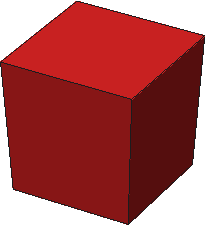
\includegraphics[width=\textwidth]{cubo}%
       	\label{subfig:cubo}%
    \end{subfigure}%
    %
    \hspace{1.5cm}
    %
    \begin{subfigure}[b]{0.2\textwidth}
       	\includegraphics[width=\textwidth]{prisma}%
       	\label{subfig:prisma}%
    \end{subfigure}%
    %
    \caption{Ejemplos de los objetos considerados para las clases $C_1$ (izquierda) y $C_2$ (derecha).}%
    \label{fig:objetos}%
\end{figure}
%
De los atributos posibles de estos objetos, el utilizado para diferenciar las clases de objetos es su altura $h$, el cual es suficiente para abordar el problema.

Así:
%
\begin{align}
	\label{eq:atributos_diferenciadores}
	A_k &= \{h_k\} \\
	\intertext{son los conjuntos de atributos asociados a cada objeto $o_k$, donde $h_k$ solo puede tener dos posibles valores, por lo cual las clases quedan definidas de la siguiente forma:}
	\begin{split}
		C_1  &= \{h_1\} \\[1em]
		C_2  &= \{h_2\} \rlap{${}= \{2h_1\}$}
	\end{split}
\end{align}
%
Para evaluar la propuesta en las diferentes configuraciones propuestas del espacio $E$, se utilizaron diferentes cantidades de objetos, siendo $N$ la cantidad total de objetos en dichos espacios, la cual será la suma de los objetos de ambas clases propuestas, donde $N_1$ es la cantidad de objetos de la clase $C_1$ y $N_2$ los objetos de la clase $C_2$. 

En los casos tratados solo se permite colocar un objeto por cada celda de la malla y la cantidad $N$ debe cumplir la desigualdad $\left\lceil \frac{nm}{2} \right\rceil < N \leq nm$.
Esto porque una cantidad de objetos igual o menor a $\left\lceil \frac{nm}{2} \right\rceil$ se considera un caso con solución trivial; ya que siempre se dispone de espacio suficiente para acomodarlos en una configuración en la cual se puedan tomar con una sola acción.
Además, el número de objetos disponibles no debe exceder el número total de celdas.
 
Dicho lo anterior, los casos de interés para validar la propuesta de este trabajo, consisten en todas las configuraciones de objetos $N_1$ y $N_2$ que no correspondan a casos triviales ni imposibles (los cuales serán detallados en la Sección \ref{sec:casos_triviales_e_imposibles}).
Es por ello que se obtuvieron las condiciones para que un caso no sea trivial ni imposible, resultando las siguientes:
%
\begin{equation}
\label{eq:cond_casos_de_interes}
\begin{gathered}
	\left\lceil \frac{nm}{2} \right\rceil < N \leq nm \\[7pt]
	N = N_1 + N_2 \\[7pt]
	0 \leq N_1 \leq N - \left\lfloor \frac{n}{2} \right\rfloor \! \left\lfloor \frac{m}{2} \right\rfloor \\[7pt]
	0 \leq N_2 \leq N - \left\lfloor \frac{n}{2} \right\rfloor \! \left\lfloor \frac{m}{2} \right\rfloor
\end{gathered}
\end{equation}
%
Un análisis más profundo de estas condiciones se dará en la Sección \ref{sec:casos_triviales_e_imposibles}.
%
%
\subsection{Características de la vecindad}
\label{subsec:vecindad}
%
%
Para definir el estado de la vecindad $V_{ij}$ de una celda $e_{ij}$, se considerarán como celdas vecinas de una celda particular $e_{ij}$, aquellas celdas que se encuentran inmediatamente arriba (dirección positiva de $i$), abajo, a la derecha (dirección positiva de $j$) y a la izquierda de esta, como se ilustra en la Figura \ref{fig:vecindad}.
%
\begin{figure}[H]
	\includegraphics[width=0.6\textwidth]{vecindad}%
	\caption{Vecindad utilizada para abordar el problema planteado.}%
	\label{fig:vecindad}%
\end{figure}
%
El orden en el que se encuentran los estados de las celdas vecinas en el conjunto $V_{ij}$ se obtiene recorriendo las posiciones mencionadas en sentido horario comenzando con la celda de arriba, es decir:
%
\begin{equation}
	\label{eq:vecindad_usada}
	V_{ij} = \{v_1, v_2, v_3, v_4\}
\end{equation}
%
donde:
%
\begin{descriptionParams}
	\item[$v_1$] corresponde al estado de la celda $e_{i+1,\, j}$.
	\item[$v_2$] corresponde al estado de la celda $e_{i,\, j+1}$.
	\item[$v_3$] corresponde al estado de la celda $e_{i-1,\, j}$.
	\item[$v_4$] corresponde al estado de la celda $e_{i,\, j-1}$.
\end{descriptionParams}
%
Las características de la vecindad de los elementos en los bordes y esquinas de la malla no difiere de las de los demás elementos.
Esto debido a que en todos los arreglos tratados se considera un ``espacio extendido'' de trabajo, el cual consiste en suponer que el espacio $E$ se encuentra rodeado por celdas vacías, tal y como se muestra en la Figura \ref{fig:malla_extendida}.
En estas celdas hipotéticas no se puede colocar ningún objeto, ya que únicamente cumplen con la función de actuar como vecinas de los elementos en los bordes y esquinas de la malla, de manera que las mismas reglas de vecindad de los elementos centrales también puedan ser aplicadas en ellos.
%
\begin{figure}[H]
	\includegraphics[width=0.6\textwidth]{malla_extendida_3D}%
	\caption{Ejemplo de espacio extendido en una malla de $4\times 4$.}%
	\label{fig:malla_extendida}%
\end{figure}
%
En todos los casos del presente trabajo se supondrá un espacio extendido como el de la Figura \ref{fig:malla_extendida}, pero esta característica puede ser modificada según las necesidades del problema que se aborde.
Por ejemplo, si se desea realizar el acomodo de objetos dentro de una caja, puede ser más adecuado cambiar las celdas vacías del espacio extendido por elementos fijos de determinada altura, a manera de pared.
%
%
\subsection{Formas de sujeción}
\label{subsec:formas_sujecion}
%
%
Solo se consideran dos formas de agarre, las cuales son comunes a ambas clases de objetos: agarre horizontal $H$ y agarre vertical $V$; esto es:
%
\begin{equation}
\label{eq:formas_sujecion_usadas}
	S = S_1 = S_2 = \{H, V\}
\end{equation}
%
Estas formas de agarre se establecieron considerando un manipulador que solo puede tomar los objetos por la parte superior. 
Un esquema de los puntos que son utilizados, en teoría, para sujetar los objetos se muestra en la Figura \ref{fig:formas_sujecion}.
%
\begin{figure}[H]
	\begin{subfigure}{0.4\textwidth}
		\includegraphics[width=\textwidth]{agarre_horizontal}%
		\label{subfig:sujecion_H}%
	\end{subfigure}%
	%
	\hspace{1cm}
	%
	\begin{subfigure}{0.4\textwidth}
		\includegraphics[width=\textwidth]{agarre_vertical}%
		\label{subfig:sujecion_V}%
	\end{subfigure}%
	\caption{Formas de sujeción horizontal (izquierda) y vertical (derecha).}%
	\label{fig:formas_sujecion}%
\end{figure}
%
%
\subsection{Restricciones de las formas de sujeción}
\label{subsec:restricciones}
%
%
Las formas de sujeción aplicables a cada clase de objeto pueden ser restringidas en función de su vecindad $V_{ij}$.
	
Un objeto $o_k$ puede ser sujetado de las formas $H$ y $V$ si sus vecinos horizontales y verticales, respectivamente, tienen una menor altura que el objeto $o_k$.
La definición matemática de la oración anterior se presenta en la Ecuación \ref{eq:restricciones} de la Sección \ref{sec:funciones_y_procedimientos}.

Algunos ejemplos de cómo se restringen las formas de sujeción de un objeto, en función de su vecindad se muestran en la Figura \ref{fig:restricciones_agarre}.
%
\begin{figure}[H]
	\def\hsep{12pt}%
	\captionsetup[subfigure]{width=\textwidth}%
	\begin{subfigure}{0.31\textwidth}
		\includegraphics[width=\textwidth]{restriccion_H_cubo}%
		\label{subfig:restriccion_H_cubo}%
	\end{subfigure}%
	\hspace{\hsep}%
	\begin{subfigure}{0.31\textwidth}
		\includegraphics[width=\textwidth]{restriccion_V_cubo}%
		\label{subfig:restriccion_V_cubo}%
	\end{subfigure}%
	\hspace{\hsep}%
	\begin{subfigure}{0.31\textwidth}
		\includegraphics[width=\textwidth]{restriccion_HV_cubo}%
		\label{subfig:restriccion_HV_cubo}%
	\end{subfigure}%
	
	\vspace{0.7cm}
	%
	\begin{subfigure}{0.31\textwidth} 
		\includegraphics[width=\textwidth]{restriccion_H_prisma}%
		\label{subfig:restriccion_H_prisma}
	\end{subfigure}%
	\hspace{\hsep}%
	\begin{subfigure}{0.31\textwidth}
		\includegraphics[width=\textwidth]{restriccion_V_prisma}%
		\label{subfig:restriccion_V_prisma}
	\end{subfigure}%
	\hspace{\hsep}%
	\begin{subfigure}{0.31\textwidth}
		\includegraphics[width=\textwidth]{restriccion_HV_prisma}%
		\label{subfig:restriccion_HV_prisma}%
	\end{subfigure}%
	%
	\caption{Ejemplos de cómo se pueden restringir las formas de sujeción en función de la vecindad.}%
	\label{fig:restricciones_agarre}%
\end{figure}
%
%
\subsection{Acciones}
\label{subsec:acciones}
%
%	
Por el momento solo se consideran dos tipos de acciones: poner un objeto en $E$ ($w_1$) y quitarlo de $E$ ($w_2$), es decir:
%
\begin{equation}
	\label{eq:acciones_usadas}
	W = \{w_1, w_2\}
\end{equation}
%
Se considera que estas acciones son suficientes para la primera aproximación propuesta para el problema planteado. 
%
%
\subsection{Especificaciones adicionales}
\label{subsec:especificaciones_adicionales}
%
%	
Los objetos no se pueden colocar uno encima de otro, por lo cual solo se pueden generar acomodos como el que se muestra en la Figura \ref{fig:muestra_acomodo}.
	
A diferencia del problema del contenedor, no se toma en cuenta el caso en que haya que dejar objetos sin acomodar por falta de espacio.
Ya que, si bien este sería un caso de estudio interesante, en el que se podrían fusionar las técnicas del problema del contenedor con las propuestas, se cree que el añadir este tipo de restricciones disfrazaría la esencia del verdadero problema que se quiere resolver.
Por lo cual se da por hecho que los $N$ objetos se pueden colocar sin problemas en $E$, es decir, ningún objeto debe quedar fuera de $E$ en el arreglo final.
%
\begin{figure}[H]
	\includegraphics[width=0.63\textwidth]{arreglo_muestra}%
	\caption{Ejemplo de una configuración de objetos en la malla.}%
	\label{fig:muestra_acomodo}%
\end{figure}
%
%
\section{Análisis de complejidad del problema}
\label{sec:analisis_complejidad}
%
%
Debido a que el objetivo final del presente trabajo es encontrar una configuración específica de los objetos de $O$ en $E$, la complejidad del problema estará entonces relacionada con el total de configuraciones de objetos que se pueden generar a partir de dados: un conjunto $O$ de objetos y un espacio $E$ en el cual colocarlos.  

Si se considera el espacio de búsqueda sobre todas las configuraciones posibles de objetos en la malla, utilizando el conjunto $O$ para la representación de los objetos y el símbolo $\boxslash$ para la representación de una celda vacía, se tiene el siguiente espacio de búsqueda:
%
\begin{equation}
	\label{eq:complejidad_1}
	\mathcal{C} = (O \cup \{ \boxslash \})^{nm}
\end{equation}
%
donde se ha hecho explícita la unión con la representación de una celda vacía, al considerarla como un elemento más del conjunto, debido a su recurrente uso.

Al utilizar el conjunto $O$ para la representación de los objetos, implícitamente se está considerando a cada uno de sus elementos como diferente a los demás, ya que, en general, sus respectivos atributos $A_k$ pueden ser diferentes.
Por lo cual el número de configuraciones posibles en dicho espacio viene dado por: 
%
\begin{equation}
	\label{eq:complejidad_2}
	|\mathcal{C}| = |O \cup \{ \boxslash \}|^{nm} = (N+1)^{nm}
\end{equation} 
%
Con la finalidad de reducir este espacio de búsqueda es que se ha establecido el sistema de clases definido anteriormente.
Mediante esta herramienta es posible identificar atributos clave $A_k$ de objetos no necesariamente iguales, los cuales permitan tratarlos como tal únicamente en lo que respecta a su sujeción.
Por ejemplo, si al tener una esfera y un cubo en el espacio $E$ se tiene la condición de que el manipulador solo es capaz de tomar estos objetos mediante una única posición y orientación, utilizando puntos de contacto semejantes; entonces, no tendría caso considerar estos objetos como diferentes, en lo que a su manipulación se refiere.
Por lo cual, para cuestiones de sujeción, lo conveniente sería representarlos como objetos de la misma clase.

Al hacer esta consideración el espacio de búsqueda puede ser reducido, ya que:
%
\begin{equation}
	\label{eq:complejidad_3}
	|C| \leq |O|
\end{equation}
%
por lo cual el nuevo espacio de búsqueda sería:
%
\begin{equation}
	\label{eq:complejidad_4}
	\mathcal{C}' = (C \cup \{ \boxslash \})^{nm}
\end{equation}
%
Y de forma similar a la Ecuación \ref{eq:complejidad_2}, el número de configuraciones posibles quedaría como:
%
\begin{equation}
	\label{eq:complejidad_5}
	|\mathcal{C}'| = |C \cup \{ \boxslash \}|^{nm} = (N_C+1)^{nm}
\end{equation}
%
Sin embargo, el espacio de búsqueda de interés para el problema enunciado, es un subconjunto de $\mathcal{C}'$, para el cual se tiene un número de objetos $N$ fijo, e igualmente las cantidades de objetos de cada clase $N_1, N_2, \ldots, N_{N_C}$ son también fijas.

Entonces, se define $\mathcal{C}''$ como el espacio de todas las configuraciones posibles de $N$ objetos de $N_C$ clases en un $E$ específico, donde $N_1, N_2, \ldots, N_{N_C}$ son cantidades fijas.
Para lo cual se define a $\mathcal{C}''_{\text{ins}}$ como cualquier instancia de $\mathcal{C}''$ y a $\mathcal{C}''_{\text{ins}}(C_K)$ como el número de veces que aparece la clase $C_K$ en $\mathcal{C}''_{\text{ins}}$.
Por lo tanto 
%
\begin{equation}
	\label{eq:complejidad_6}
	\mathcal{C}'' = (C \cup \{ \boxslash \})^{nm} \ | \ \mathcal{C}''_{\text{ins}}(C_K) = N_K,\ 1 \leq K \leq N_C
\end{equation}
%
lo cual establece que debe haber exactamente $N_1$ objetos de la clase $C_1$, $N_2$ de la clase $C_2$, etc., en cualquier instancia de $\mathcal{C}''$.

El número de configuraciones posibles para $\mathcal{C}''$ es entonces:
%
\begin{equation}
	\label{eq:complejidad_7}
	|\mathcal{C}''| = \frac{nm!}{N_1!N_2! \cdots N_{N_C}!(nm - N)!}
\end{equation}
%
En la Tabla \ref{tab:permutaciones_posibles} se muestra el número de configuraciones posibles para algunas combinaciones de valores del tamaño de la malla y del número de objetos de cada clase.
%
\begin{table}[H]
	\renewcommand{\arraystretch}{1.4}%
	\savetablewidth{%
	\begin{tabular}{ccccc}
		\hline
		\textbf{Tamaño malla} & $\bm{N_1}$ & $\bm{N_2}$ & $\bm{nm-N}$ & $\bm{|\mathcal{C}''|}$ \\ \hline
		\arrayrulecolor{gray!60}%
		$3\times 3$ & $3$ & $3$ & $3$ & $\num{1680}$ \\ \hline
		$3\times 3$ & $1$ & $5$ & $3$ & $504$ \\ \hline
		$3\times 3$ & $4$ & $5$ & $0$ & $126$ \\ \hline
		$4\times 4$ & $5$ & $5$ & $6$ & $\num{2018016}$ \\ \hline
		$4\times 4$ & $1$ & $9$ & $6$ & $\num{80080}$ \\ \hline
		$4\times 4$ & $8$ & $8$ & $0$ & $\num{12870}$ \\ \hline
		$5\times 5$ & $8$ & $8$ & $9$ & $2.62\times10^{10}$ \\ \hline
		$5\times 5$ & $10$ & $10$ & $5$ & $0.98\times10^{10}$ \\ \hline
		$5\times 5$ & $12$ & $13$ & $0$ & $\num{5200300}$ \\ \hline
		$6\times 6$ & $12$ & $12$ & $12$ & $3.38\times10^{15}$ \\ \hline
		$6\times 6$ & $15$ & $15$ & $6$ & $0.30\times10^{15}$ \\ \hline
		$6\times 6$ & $18$ & $18$ & $0$ & $9.07\times10^{9}$ \\ 
		\arrayrulecolor{maintextcolor}%
		\hline
	\end{tabular}%
	}%
	\captionsetup{width=\tablewidth}%
	\caption{Número de permutaciones de arreglos posibles en función del número de elementos de cada clase presentes en la malla y del tamaño de la malla.}%
	\label{tab:permutaciones_posibles}%
\end{table}
%
Al analizar la Tabla \ref{tab:permutaciones_posibles} se puede observar que, entre más uniforme sea la distribución del número de objetos de cada clase y de celdas vacías ($nm - N$), el número de permutaciones posibles de una malla aumenta.
Es decir, que cuando las cantidades de objetos de cada clase y de celdas vacías son lo más parecidas entre sí, es cuando el número de permutaciones es máximo, y disminuye conforme se va perdiendo esta uniformidad.
%
%
\section{Casos triviales y casos imposibles}
\label{sec:casos_triviales_e_imposibles}
%
%
Existen cantidades especiales de objetos $N$, así como del número de objetos de cada clase $N_1, N_2, \ldots, N_{N_C}$, para las cuales se pueden tener casos de acomodo triviales o imposibles.
Las características de estos casos se definen a continuación.

Un caso trivial es un caso en el cual la cantidad $N$ de objetos es lo suficientemente pequeña como para acomodar los objetos en un patrón simple, el cual permite que todos los objetos puedan ser sujetados con una sola acción.
En este caso los objetos pueden ser siempre colocados mediante un mismo patrón, previamente establecido, siempre que se cumpla la siguiente condición:
%
\begin{equation}
	\label{eq:condicion_triviales}
	N \leq \left\lceil \frac{nm}{2} \right\rceil
\end{equation}
%
Un patrón de acomodo para casos triviales se presenta en la Figura \ref{fig:casos_triviales}, dónde $N = \left\lceil \frac{nm}{2} \right\rceil$.
En el presente trabajo no se abordan este tipo de casos.
%
\begin{figure}[H]
    \begin{subfigure}{0.3\textwidth}
		\includegraphics[width=\textwidth]{arreglo_trivial_4x4_2D}%
       	\label{subfig:trivial_4x4}%
    \end{subfigure}%
    %
    \hspace{2.2cm}
    %
    \begin{subfigure}{0.3\textwidth}
       	\includegraphics[width=\textwidth]{arreglo_trivial_5x5_2D}%
       	\label{subfig:trivial_5x5}%
    \end{subfigure}%
    %
    \caption{Ejemplos de casos triviales en mallas de $4\times 4$ (izquierda) y $5\times 5$ (derecha).}
    \label{fig:casos_triviales}%
\end{figure}
%
Por otro lado, también existen configuraciones específicas de objetos en la malla, las cuales implican que algunos objetos sean imposibles de tomar, dadas las reglas de sujeción establecidas.
Estos casos se presentan cuando al menos cuatro objetos de la misma clase se agrupan en un patrón como el que se muestra en la subfigura izquierda de la Figura \ref{fig:casos_imposibles}.
En este caso ninguno de los cuatro objetos puede ser sujetado mediante las formas de sujeción definidas $H$ y $V$.
Estas agrupaciones de cuatro elementos de la misma clase se puede presentar una o varias veces en un acomodo de objetos, como se muestra en la subfigura derecha de la Figura \ref{fig:casos_imposibles}.

Se ha denominado como \textsl{cuadro imposible} al arreglo de cuatro objetos de la misma clase descrito anteriormente, y como \textsl{caso imposible} a un arreglo de objetos en la malla que contenga al menos un cuadro imposible.
%
\begin{figure}[H]
	\begin{subfigure}{0.3\textwidth}
		\includegraphics[width=\textwidth]{arreglo_imposible1_4x4_2D}%
   		\label{subfig:imposibles_1}%
	\end{subfigure}%
	%
	\hspace{2.2cm}
	%
	\begin{subfigure}{0.3\textwidth}
		\includegraphics[width=\textwidth]{arreglo_imposible2_4x4_2D}%
		\label{subfig:imposibles_2}%
	\end{subfigure}%
	%
	\caption{Ejemplos de casos imposibles.}%
	\label{fig:casos_imposibles}%
\end{figure}
%
Los casos imposibles como los de la Figura \ref{fig:casos_imposibles} se pueden evitar con un acomodo correcto de los objetos en la malla.
Sin embargo existe una condición, la cual implica que siempre habrá cuadros imposibles en la malla, sin importar la forma en que se acomoden los objetos.

La condición para que exista al menos un cuadro imposible en un arreglo de objetos es:
%
\begin{equation}
	\label{eq:condicion_imposibles}
	\max_{K} N_K > nm - \left\lfloor \frac{n}{2} \right\rfloor \! \left\lfloor \frac{m}{2} \right\rfloor
\end{equation}
%
En el presente trabajo no se abordan este tipo de casos.

En el siguiente capítulo se presentarán los procedimientos y algoritmos desarrollados para abordar el problema propuesto.
Al final del capítulo se presentará el algoritmo principal que resuelve el problema planteado, el cual hace uso de los procedimientos que le preceden.
Posteriormente, en el Capítulo \ref{chap:resultados}, se presentarán los resultados obtenidos al aplicar el algoritmo principal a diferentes tamaños de malla y diferentes combinaciones de cantidades de objetos en ellas.
Finalmente, en el Capítulo \ref{chap:conclusiones}, se abordarán las conclusiones del proyecto.
% !TEX encoding = UTF-8 Unicode
\chapter{Metodología propuesta}
\label{chap:propuesta}
%
%
En este capítulo se establecerá y detallará la propuesta para realizar un acomodo de objetos, con la condición de minimizar el número de acciones que conlleva el acceder a cada uno de ellos.
Dicha propuesta se basa en un sistema de puntuaciones, asignadas a cada uno de los elementos en la malla incluyendo celdas vacías.
La puntuación que se asignará a cada elemento dependerá de la clase del elemento en cuestión así como de su vecindad.

La puntuación de un elemento, cuando se trate de un objeto, será máxima cuando este se pueda tomar mediante una sola acción y disminuye con la presencia de vecinos que impiden su agarre o sujeción.
En el caso de las celdas vacías, su puntuación se incrementa con respecto al número de celdas vecinas que sean ocupadas por objetos, y disminuye en función del número de celdas vecinas vacías.

Con este sistema de puntuaciones, el cual es parte fundamental de las aportaciones de la propuesta aquí presentada, se busca que la puntuación global de la malla, esto es, la suma de las puntuaciones de los elementos individuales, sea máxima; lo cual es sinónimo de un fácil acceso y posterior sujeción de los objetos.

Los procesos para calcular las puntuaciones mencionadas son integrados en una función, la cual es a su vez utilizada por un algoritmo de recocido simulado, en el cual convergen las aportaciones de este trabajo y que se encarga de hacer los cambios necesarios a un acomodo inicial aleatorio, con la finalidad de que la puntuación global se maximice.
De esta forma es como se obtendrá un acomodo de objetos optimizado para realizar el acceso y la sujeción de cada uno de los objetos en una malla, con un número de acciones mínimas en promedio, lo cual en la práctica también podría implicar un tiempo mínimo promedio para acceder a los objetos.
Para ello se evalúan los acomodos obtenidos por el algoritmo al calcular el costo de tomar cada objeto de la malla mediante una función de costo.

La definición completa del algoritmo y de las funciones mencionadas se dará en las siguientes secciones.
%
%
\section{Funciones y procedimientos propuestos}
\label{sec:funciones_y_procedimientos}
%
%
En esta sección se iniciará con la definición de los componentes más básicos de la metodología propuesta, posteriormente se definirán las funciones y procedimientos de más alto nivel, que hacen uso de dichos componentes y finalmente, en la Sección \ref{sec:algoritmo_principal}, se describirá el algoritmo principal de la propuesta, el cual es la definición de más alto nivel de esta.

Con la finalidad de simplificar la notación de algunos cálculos posteriores, se define $C_0$ como la clase de una celda vacía, la cual, al solo tener fines de representación, no tiene ningún atributo asociado.
Asimismo se define $h_{ij}$ como la altura del elemento en la celda $e_{ij}$, definiendo la altura de una celda vacía como cero.

Se define la función de estado $C_{ij}$ como la función que retorna la clase del elemento posicionado en la celda $e_{ij}$.
%
\begin{equation}
	C_{ij} \mapsto C \cup \{ C_0 \}
\end{equation}
%
Además, se define la función de sujeción $S_{ij}$ como la función que retorna el subconjunto de formas de sujeción permitidas de un objeto posicionado en la celda $e_{ij}$.
%
\begin{equation}
	S_{ij} \mapsto S'_K \hspace{1pt}, \qquad S'_K \subseteq S_K
\end{equation}
%
Las expresiones que describen las condiciones bajo las cuales los objetos pueden ser sujetados, correspondientes a la descripción dada en la Sección \ref{subsec:restricciones}, se presentan a continuación:
%	
\begin{equation}
\label{eq:restricciones}
	\begin{aligned}
		&h_{i+1,\, j} < h_{ij}\ \wedge\ h_{i-1,\, j} < h_{ij}\ \Rightarrow\ H \in S_{ij} \\[0.7em]
		&h_{i,\, j+1} < h_{ij}\ \wedge\ h_{i,\, j-1} < h_{ij}\ \Rightarrow\ V \in S_{ij}
	\end{aligned}
\end{equation}
%
Por lo tanto, la condición para que un objeto en una celda $e_{ij}$ sea sujetable es simplemente:
%
\begin{equation}
\label{eq:sujetable}
	|S_{ij}| \geq 1
\end{equation}
%
Con fines de legibilidad en definiciones posteriores, se utilizará la función booleana $\f{sujetable}(e_{ij})$, la cual simplemente indica si para el elemento de la celda $e_{ij}$ se cumple o no la condición de la Ecuación \ref{eq:sujetable}.
De forma similar, la función $\f{imposible}(e_{ij})$ indica si el elemento en la celda $e_{ij}$ pertenece a un cuadro imposible, como los que se describen en la Sección \ref{sec:casos_triviales_e_imposibles}.
%
%
\subsection{Funciones de ponderación}
\label{subsec:funciones_ponderacion}
%
%
A continuación se presenta la función que asigna una puntuación (un número entero) a un par de elementos vecinos en $E$.

Algo a tener en cuenta con esta función es que, si bien por si sola es una función que solo puntúa un par de elementos en la malla, está pensada para ser una sub-función del proceso de puntuación de más alto nivel de la Función \ref{func:puntuacion_elemento}, enfocado a puntuar un elemento particular de la malla en función de su vecindad.
Particularmente es el elemento del primer argumento de la Función \ref{func:puntuacion_par} el que será puntuado respecto a su vencindad en la Función \ref{func:puntuacion_elemento}.
Esta es una de las razones por las que en algunos casos el resultado de la función no sea conmutativo respecto al orden de sus argumentos, ya que en el proceso de puntuación de más alto nivel se le da más ``atención'' al primer argumento de la función, al ser considerado como el elemento a puntuar.
%
\begin{center}
\begin{minipage}{0.9\textwidth}
\begin{function}[H]
	\OneHalfBlankLine
	\Data{Celdas de los elementos vecinos $e_{i_1 j_1}$, $e_{i_2 j_2}$.}
	\Result{Puntuación.}
	\OneHalfBlankLine
	\Function{$\f{puntuacionPar}(e_{i_1 j_1}$, $e_{i_2 j_2})$}{
		\HalfBlankLine
		\Switch{$C_{i_1 j_1}$, $C_{i_2 j_2}$}{
			\HalfBlankLine
			\lCase{$C_1$, $C_0$}{\Return 3}
			\lCase{$C_1$, $C_2$}{\Return 1}
			\lCase{$C_2$, $C_1$}{\Return 2}
			\lCase{$C_2$, $C_0$}{\Return 1}
			\lCase{$C_0$, $C_1$}{\Return 2}
			\lCase{$C_0$, $C_2$}{\Return 1}
			\lCase{$C_{k_C}$, $C_{k_C}$}{\Return 0}
		}
	}
	\caption{puntuacionPar($e_{i_1 j_1}$, $e_{i_2 j_2}$). Función para obtener la puntuación de un par de elementos vecinos.}%
	\label{func:puntuacion_par}%
\end{function}
\end{minipage}
\end{center}
%
El sistema de puntuación presentado en la Función \ref{func:puntuacion_par} fue diseñado en base a heurísticas simples, esto con el propósito de que su implementación fuese eficiente en términos de velocidad de procesamiento.
Sin embargo, se intentó mantener un balance entre la eficiencia en el número de operaciones, proporcionada por la simpleza de las reglas de puntuación; y la eficiencia de los arreglos encontrados por el algoritmo, que está definida en términos del número total de acciones necesarias para tomar los objetos.

Dicho lo anterior, y teniendo en cuenta que posteriormente el primer argumento de la Función \ref{func:puntuacion_par} fungirá como el elemento a ser puntuado en la Función \ref{func:puntuacion_elemento}, las heurísticas detrás del sistema de puntuación utilizado en la Función \ref{func:puntuacion_par} son las siguientes:
%
\begin{itemize}
	\item Para los cubos (casos $C_1$, $C_0$ y $C_1$, $C_2$): la puntuación es máxima cuando su vecino es una celda vacía, debido a que es el elemento que puede permitir su sujeción; y es mínima, pero no cero, cuando su vecino es un prisma, ya que, si bien se restringe la sujeción del cubo, aún hay posibilidad de que el prisma sí pueda ser sujetable.
	\item Para los prismas (casos $C_2$, $C_1$ y $C_2$, $C_0$): la puntuación es máxima cuando su vecino es un cubo, pero no tanto como la del par \textsl{cubo-celda\,vacía}.
	La razón de esto es que, si bien la sujeción del prisma no se restringe, la del cubo sí, mientras que en el caso del par \textsl{cubo-celda\,vacía} no se genera ninguna restricción de sujeción.
	Por otro lado, la puntuación es mínima, pero no cero, cuando el vecino de un prisma es una celda vacía; esto debido a que, si bien la sujeción del prisma no se restringe, es posible que la celda vacía pueda ser mejor aprovechada al colocarla al lado de un cubo.
	\item Para las celdas vacías (casos $C_0$, $C_1$ y $C_0$, $C_2$): la puntuación es máxima cuando su vecino es un cubo, debido a que la celda vacía es el único elemento que permite su sujeción; y es mínima, pero no cero, cuando su vecino es un prisma, ya que permite su sujeción pero también existe otro elemento que la permite, pudiendo ser una mejor elección en determinadas situaciones.
	\item Para vecinos de la misma clase (caso $C_{k_C}$, $C_{k_C}$): la puntuación es cero.
	 La razón de ello es que, tratándose de objetos, se restringe la sujeción de ambos, mientras que si se trata de celdas vacías, su capacidad para permitir la sujeción de objetos es desaprovechada.
\end{itemize}
%
Otra de las razones para que la función no sea conmutativa, en el caso de vecinos de clase $C_1$ y $C_0$, es para no dar una preferencia excesiva a los pares de vecinos de estas clases, ya que esto puede causar que se generen pares innecesarios de este tipo en el arreglo.
Por ejemplo, se podría generar una tendencia a hacer sujetables a los cubos mediante sus dos formas de sujeción $H$ y $V$.
Con esto se podría desaprovechar el uso de espacios vacíos solo en cubos en situaciones donde el número de prismas sea mayor y se requieran pares \textsl{prisma-celda\,vacía}.

En el caso de vecinos de clase $C_1$ y $C_2$ la razón es más evidente y tiene que ver con el elemento que se está puntuando, ya que en un caso no se restringe la sujeción de dicho elemento y en el otro sí.

La puntuación de un elemento en una celda $e_{ij}$ de la malla es calculada por la Función \ref{func:puntuacion_elemento}, haciendo uso de la Función \ref{func:puntuacion_par}.
Cuando el elemento corresponde a un objeto y este es sujetable, se calculan las puntuaciones con sus vecinos horizontales y verticales, estas dos puntuaciones se comparan y la puntuación que resulte mayor es la que se asigna al elemento, añadiendo puntos extra; si el objeto no es sujetable, su puntuación solo es la suma de las puntuaciones con sus cuatro vecinos, restando puntos si el elemento es imposible de tomar.
Si el elemento a puntuar se trata de una celda vacía, simplemente se suman las puntuaciones con sus cuatro vecinos, sin realizar ninguna operación adicional.

El proceso detallado para puntuar un elemento de la malla se muestra a continuación en la Función \ref{func:puntuacion_elemento}.
Las funciones $\f{sujetable}()$ e $\f{imposible}()$ se describen al inicio de la Sección \ref{sec:funciones_y_procedimientos}.
%
\begin{center}
\begin{minipage}{0.9\textwidth}
\begin{function}[H]
	\OneHalfBlankLine
	\Data{Celda del elemento a puntuar $e_{ij}$.}
	\Result{Puntuación $p$ del elemento.}
	\OneHalfBlankLine
	\Function{$\f{puntuacionElemento}(e_{ij})$}{
		\BlankLine
		$p_H = \f{puntuacionPar}(e_{ij},\: V_{i, j, 2}) +\, \f{puntuacionPar}(e_{ij},\: V_{i, j, 4})$\;
		\QuarterBlankLine
		$\mathrlap{p_V}\hphantom{p_H} = \f{puntuacionPar}(e_{ij},\: V_{i, j, 1}) +\, \f{puntuacionPar}(e_{ij},\: V_{i, j, 3})$\;
		\BlankLine
		$p = p_H + p_V$\;
		\OneHalfBlankLine
		\If{$C_{ij} \neq C_0$}{
			\BlankLine
			\lIf{$\mathrlap{\f{sujetable}(e_{ij})}\hphantom{\f{imposible}(e_{ij})}$}{$p\ \!\!= \max(p_H,\: p_V) + 3$}
			\QuarterBlankLine
			\lIf{$\f{imposible}(e_{ij})$}{$p\ -\!\!= 2$}
			\HalfBlankLine
		}
		\BlankLine
		\Return $p$
		\HalfBlankLine
	}
	\caption{puntuacionElemento($e_{ij}$). Función para calcular la puntuación de un elemento de la malla.}%
	\label{func:puntuacion_elemento}%
\end{function}
\end{minipage}
\end{center}
%
Finalmente, se define la puntuación global de la malla como la suma de las puntuaciones individuales de todos sus elementos:
%
\begin{equation}
\f{puntuacionGlobal}() = \sum_{i,\hspace{1pt} j}\, \f{puntuacionElemento}(e_{ij})
\end{equation}

\vspace{-\belowdisplayskip}%
%
%
\subsection{Costo de tomar los objetos}
\label{subsec:costo}
%
%
El algoritmo para calcular el costo $t_{ij}$ de tomar un objeto de la malla está basado en el algoritmo RSC, presentado en \cite{4209604}.
Dicho algoritmo consiste básicamente en crear un árbol de objetos-obstáculo que impiden la sujeción de un objeto particular. 
La raíz del árbol es el objeto que se desea tomar, y a partir de este, se ramifican nodos correspondientes a sus objetos-obstáculo más inmediatos.
A su vez, de cada uno de estos nodos se desprenden más ramas o nodos, correspondientes a los objetos-obstáculo de cada uno, y así sucesivamente hasta llegar a las hojas del árbol, las cuales corresponden a objetos-obstáculo que sí son sujetables.

Al retirar los objetos correspondientes a los nodos hoja, se pueden hacer sujetables los objetos de sus nodos padres, con lo cual se convierten en nuevos nodos hoja, reduciendo el tamaño del árbol de objetos-obstáculo.
Al continuar con este proceso se puede hacer sujetable al objeto del nodo raíz.
%
\begin{figure}[H]
\includegraphics{arbol}%
\caption{Ejemplo de arreglo de objetos (izquierda) y el árbol de objetos-obstáculo correspondiente al cubo A (derecha). Como se puede observar, la solución óptima para tomar este cubo tiene costo 3.}%
\label{fig:arbol}%
\end{figure}
%
De acuerdo con las formas de sujeción establecidas, existen en general, dos secuencias distintas de objetos-obstáculo que hay que retirar de la malla para hacer sujetable a otro objeto particular. 
El costo $t_{ij}$ para tomar un objeto en la celda $e_{ij}$ es entonces la longitud de la secuencia con menos objetos a retirar, tal como se muestra en la Figura \ref{fig:arbol}, donde esta secuencia corresponde a la rama de menor longitud del árbol generado.
El cálculo de $t_{ij}$ se detalla en el Algoritmo \ref{alg:costo_individual}, el cual utiliza la Función \ref{fun:secuencia} recursiva.

La Función \ref{fun:secuencia} implementa un algoritmo de \textit{backtracking} para encontrar una de las secuencias de objetos-obstáculo para hacer sujetable y tomar un objeto de interés.
La secuencia encontrada por la función es considerada como solución al problema de hacer sujetable y tomar un objeto, esto debido a que él o los elementos al final de la secuencia siempre corresponderán a nodos hoja en el árbol de objetos-obstáculo del objeto de interés, como el que se muestra en Figura \ref{fig:arbol}.
Al retirar estos objetos, se harán sujetables los siguientes objetos de la secuencia y así sucesivamente hasta hacer sujetable al primer elemento de la secuencia, el cual corresponde al objeto que se desea tomar.

El algoritmo de \textit{backtracking} explora las ramas del árbol de objetos-obstáculo de un objeto particular y determina si al final de la rama existen objetos sujetables o no.
Si no es posible retirar ningún objeto de la rama en cuestión, la función falla.
Esto sucede cuando el elemento de la malla que se está analizando ya se encuentra agregado en la secuencia, lo cual puede ser indicativo de la existencia de un cuadro imposible en el arreglo.
Al fallar una función, todos sus procesos y los de las funciones en recursiones previas que la llamaron directa o indirectamente se invalidan, lo cual se traduce en que la secuencia que se había estado construyendo hasta ese momento sea descartada.
Después de esto se procede a explorar otra rama del árbol. 

La primera rama para la cual la función finalice con éxito es la que se toma como solución y cuyos objetos son añadidos a la secuencia considerada como resultado de la función.
%
\begin{center}
\begin{minipage}{0.90\textwidth}
\begin{function}[H]
	\BlankLine
	\Data{Celda $e_{ij}$ del objeto deseado y lista vacía $l$.}
	\QuarterBlankLine
	\Result{Lista $l$ con la secuencia de elementos a retirar.}
	\BlankLine
	\Definitions{
		\begin{definitions}[leftmargin=\leftmargin + \widthof{$o_{ij}$} + \labelsep]
			\item[$h_{ij}$] altura del elemento en la celda $e_{ij}$.
			\item[$o_{ij}$] \justify información de interés (clase y ubicación) del objeto en la celda $e_{ij}$ que será añadida a la secuencia.
		\end{definitions}
	}
	\BlankLine
	\Function{$\f{secuencia}(e_{ij},\: l)$}{%
	\BlankLine
		\lIf{$C_{ij} = C_0$}{Finalizar recursión con éxito.}
		\BlankLine
		\eIf{$o_{ij} \not\in l$}{
			\OneHalfBlankLine
			$\f{append}(o_{ij},\: l)$
			\OneHalfBlankLine
			\uIf{$\f{sujetable}(e_{ij})$}{
				\BlankLine
				Finalizar recursión con éxito.
				\HalfBlankLine
			}
			\SetArgSty{normaltext}
			\tcp*[l]{Ejecutar uno de los siguientes pares de recursiones:}
			\uElseIfWithNoThen{Par 1:}{
				\HalfBlankLine
				\lIf{$h_{i+1,\, j} \geq h_{ij}$}{$\f{secuencia}(e_{i+1,\, j},\: l)$}
				\lIf{$h_{i-1,\, j} \geq h_{ij}$}{$\f{secuencia}(e_{i-1,\, j},\: l)$}
				\HalfBlankLine
			}
			\uElseIfWithNoThen{Par 2:}{
				\HalfBlankLine
				\lIf{$h_{i,\, j+1} \geq h_{ij}$}{$\f{secuencia}(e_{i,\, j+1},\: l)$}
				\lIf{$h_{i,\, j-1} \geq h_{ij}$}{$\f{secuencia}(e_{i,\, j-1},\: l)$}
			}
			\Else{
				\tcp*[l]{Si en ambos pares alguna de las dos recursiones terminó con fallo:}
				Finalizar recursión con fallo (hacer \textit{backtracking} e intentar otra alternativa (par) de recursión).
				\HalfBlankLine		
			}
		}{
			\HalfBlankLine
			Finalizar recursión con fallo (hacer \textit{backtracking} e intentar otra alternativa (par) de recursión).
			\HalfBlankLine
		}%
		\HalfBlankLine
		Finalizar recursión con éxito.
		\QuarterBlankLine
	}%
	\caption{secuencia($e_{ij}$, $l$). Función de \textit{backtracking} para obtener una secuencia de objetos a retirar para hacer sujetable y tomar un objeto en la celda $e_{ij}$, el cual también se incluye al final de la secuencia.}%
	\label{fun:secuencia}%
\end{function}
\end{minipage}
\end{center}
%
A grandes rasgos, el funcionamiento del Algoritmo \ref{alg:costo_individual} consiste en explorar todas las ramas del árbol de objetos-obstáculo generado para un objeto de interés (como el mostrado en la Figura \ref{fig:arbol}), mediante la Función \ref{fun:secuencia}, encontrando todas sus soluciones posibles; esto es, todas las secuencias de objetos-obstáculo consideradas como solución.
El algoritmo cuenta los objetos-obstáculo de cada una de las secuencias y finalmente retorna la longitud de la rama más corta.
%
\begin{center}
\begin{minipage}{0.98\textwidth}
\begin{algorithm}[H]
	\OneHalfBlankLine
	\Data{Celda $e_{ij}$ del objeto deseado.}
	\Result{Costo $t_{ij}$ de tomar el objeto en $e_{ij}$.}
	\TwoBlankLines
	\tcp*[l]{Lista para almacenar todas las secuencias posibles para tomar un objeto.}
	$L = \{ \}$\;
	\TwoBlankLines
	\tcp*[l]{Función que retorna todas las soluciones posibles de $\f{secuencia()}$.}
	$\f{encontrarTodas}()$\;
	\TwoBlankLines
	$L = \f{encontrarTodas}(\f{secuencia}(e_{ij},\: l))$\;
	\TwoBlankLines
	$t_{ij} = \min\limits_i \left| L_i \right|$\;
	\HalfBlankLine
	\caption{Algoritmo para calcular el costo $t_{ij}$.}%
	\label{alg:costo_individual}%
\end{algorithm}
\end{minipage}
\end{center}
%
El costo global $T$, como se definió en la Sección \ref{sec:definiciones_y_consideraciones}, es simplemente la suma de los costos individuales $t_{ij}$:
%
\begin{equation}
T = \sum_{i,\hspace{1pt} j} \, t_{ij}
\end{equation}

\vspace{-\belowdisplayskip}%
%
%
\section{Algoritmo principal}
\label{sec:algoritmo_principal}
%
%
La aportación principal de este trabajo consiste en un algoritmo para el acomodo de objetos en un arreglo, que minimiza, en promedio, el costo posterior de acceso a ellos, esto es, minimiza el costo global $T$ previamente definido.
Dicho algoritmo, el cual adquiere sus fortalezas de todas las definiciones y condiciones precedentes, es un algoritmo de recocido simulado que utiliza a la función $\f{puntuacionGlobal}()$ como criterio de evaluación para encontrar un acomodo adecuado de los objetos, acorde a los fines establecidos.

La definición original del algoritmo de recocido simulado se puede encontrar en el artículo \cite{doi:10.1126/science.220.4598.671}, en el cual también se puede encontrar una implementación muy parecida a la realizada en este trabajo, la cual consiste en optimizar la longitud de cableado en la colocación de chips en una tarjeta de circuitos, modelándola como un arreglo en forma de malla 2D.

En el problema propuesto se plantean una serie de restricciones o reglas, las cuales deben ser cumplidas independientemente del método que se utilice para encontrar los acomodos de objetos óptimos.
Por ejemplo, una de las reglas básicas del problema, es que siempre se debe de respetar el número de objetos de cada clase que deben estar presentes en el arreglo final, retornado como solución.
Es a partir de este tipo de restricciones y reglas, así como de las libertades que en sí mismas se establecen, que se debe elegir una metodología de solución apropiada para el problema planteado.

Una estrategia de búsqueda razonable para encontrar un arreglo de objetos óptimo es partir de un acomodo arbitrario de objetos, el cual cumpla desde un inicio con la restricción descrita del número de objetos de cada clase en la malla y realizar cambios en este que, además de que estén orientados a mejorar el arreglo de acuerdo al criterio establecido, siempre mantengan de igual forma el número de los distintos objetos en la malla del arreglo anterior.
La clave del éxito de dicha estrategia de búsqueda dependerá de los criterios bajo los cuales se realicen dichos cambios y de cómo estos cumplirán con las restricciones del problema.
En este caso, el criterio principal para generar tales cambios es el sistema de puntuaciones propuesto.

Se eligió un algoritmo de recocido simulado para abordar el problema propuesto debido a que se adecúa muy bien a la búsqueda de vecindad planteada para este problema, la cual consiste en cambios graduales o mínimos en un arreglo dado, considerado como solución actual.
Dichos cambios graduales se refieren a los intercambios de pares de elementos en un arreglo, ya que, bajo las reglas establecidas, un intercambio de un par de elementos distintos en un arreglo se considera como el cambio mínimo necesario para hacerlo cambiar de estado, sin alterar el número de objetos de cada clase que hay en él.

Si bien puedieran existir mejores soluciones, al emplear otro tipo de algortimos o metodologías, el objetivo principal de este trabajo no es encontrar la solución más eficiente, sino encontrar o diseñar una solución aceptable al problema propuesto, del cual no parece haber antecedentes según la investigación realizada.
Se cree que, debido al nivel de simplificación y de condiciones particulares que requiere problema, encontrar el método de solución más eficiente no sería de mucha utilidad (más allá de la intelectual) en esta etapa, como si lo sería en etapas posteriores donde se pueda aplicar en situaciones reales.

No obstante, también se consideraron otros algoritmos y metodologías de búsqueda, de entre los cuales se eligió al recocido simulado por el balance entre la simpleza del método, su conocida eficiencia, además de la ya mencionada facilidad con la que se adapta a las reglas de búsqueda del problema propuesto.

Otros métodos de reconocido éxito fueron descartados al considerar que, o bien representaban un mayor costo computacional, o bien su metodología de búsqueda no se adecuaba a las características del problema.
Por ejemplo, en un algoritmo genético, se cree que los cambios en las instancias de arreglos serían más ``abruptos'' cuando se explora el espacio de búsqueda, debido a que en las recombinaciones de población se realizan muchos cambios para generar la descendencia, que pueden alejarse mucho de los arreglos padres y que, generalmente, no los mejoran en nuestro caso.
Además de que la condición en la que el número de elementos de cada clase en el arreglo se debe mantener de una recombinación a otra, es mucho más difícil de cumplir en un algoritmo genético.
Por lo cual, en dicho caso, se concluyó que no es la mejor manera de guiar la búsqueda hacia los arreglos óptimos.

En el Algoritmo \ref{alg:recocido_simulado} se presenta el algoritmo de recocido simulado utilizado.
%
\begin{center}
\begin{minipage}{0.98\textwidth}
\setlength{\interspacetitleruled}{5pt}
\begin{algorithm}[H]
	\OneQuarterBlankLine
	\Data{Temperatura inicial $T$, constantes $\alpha$, $a$, $b$, malla con objetos.}
	\HalfBlankLine
	\Result{Malla con objetos acomodados (representada por una matriz de enteros).}
	\TwoBlankLines
	%
	\tcp*[l]{Parámetros del algoritmo.}
	$T = \num{50000000}$\;
	$\mathrlap{\alpha}\hphantom{T} = 0.0000001$\;
	$\mathrlap{a}\hphantom{T} = 0.99991$\;
	$\mathrlap{b}\hphantom{T} = 1$\;
	\TwoBlankLines
	%
	\tcp*[l]{Puntajes actual y de intercambio.}
	$p_A =\, \f{puntuacionGlobal}()$\;
	$\mathrlap{p_I}\hphantom{p_A} =\, 0$\;
	\TwoBlankLines
	%
	\While{$T > \frac{b}{1 - a}$}{
		\OneHalfBlankLine
		Intercambiar aleatoriamente 2 elementos diferentes en la malla.\;
		\HalfBlankLine
		$p_I = \f{puntuacionGlobal}()$\;
		\BlankLine
		\eIf{$p_A \leq p_I$ \Or $\f{random}([0,1]) < e^{-\frac{{\scriptstyle p}_{\scriptscriptstyle A} -\, {\scriptstyle p}_{\scriptscriptstyle I}}{\alpha T}}$}{
			\HalfQuarterBlankLine
			Se acepta el intercambio.\;
			$p_A = p_I$
			\QuarterBlankLine
		}{
			\HalfBlankLine
			No se acepta el intercambio.
			\QuarterBlankLine
		}
		\BlankLine
		$T = aT + b$
		\QuarterBlankLine
	}%
	\HalfBlankLine
	\caption{Recocido simulado.}%
	\label{alg:recocido_simulado}%
\end{algorithm}
\end{minipage}
\end{center}
%
El algoritmo recibe como entrada principal una malla con los objetos acomodados de forma aleatoria. 
Después de inicializar los parámetros del algoritmo, tales como la temperatura, se inicia un proceso iterativo, en el cual, en primer lugar se calcula la puntuación global de la malla, para luego escoger dos elementos distintos en la malla de forma aleatoria e intercambiarlos de posición.
Dicho par de elementos puede ser un par \textsl{objeto~-objeto} o bien \textsl{objeto~-celda\! vacía}.
Al simular este intercambio se vuelve a calcular la puntuación global de la malla y esta se compara con la puntuación calculada antes de hacer el intercambio.
Si la puntuación después de hacer el intercambio es mejor, entonces el intercambio se acepta, de lo contrario la probabilidad de que se acepte disminuye considerablemente.
Este proceso de intercambios se repite hasta que se cumpla la condición de paro, la cual está relacionada con el decremento de la temperatura.
Finalmente, la salida del algoritmo será el acomodo encontrado.

Los parámetros iniciales mostrados en el Algoritmo \ref{alg:recocido_simulado} fueron los utilizados para generar los arreglos de mayor tamaño ($8\times 8$).
Para arreglos de menor tamaño estos parámetros se pueden relajar hasta cierto punto, sin sacrificar la calidad de los resultados.
El esquema de reducción de temperatura utilizado es el esquema aritmético-geométrico \cite{ouali2017performance}.

Si bien el proceso de ponderación de un arreglo se ideó con el fin de que el arreglo con mayor puntuación sea el óptimo, este podría no siempre ser el caso. 
Esto es debido a que existen algunos pocos casos especiales en los que, a causa de cómo están constituidas las reglas de puntuación, el algoritmo no le da la mejor puntuación al arreglo óptimo, sino a uno que tiene, en la mayoría de los casos donde se pudo corroborar, un costo global de una o dos acciones por encima del óptimo.
Estos casos especiales se pueden corregir mediante una extensión de las reglas de puntuación que considere las situaciones en las que ocurren, sin embargo, debido a que son muy poco frecuentes, se cree que la ganancia de extender las reglas es poca comparada con la complejidad añadida al modelo, por lo cual en esta ocasión no se considerará tal extensión.

Con la finalidad de evaluar el desempeño de dicho proceso de ponderación y del algoritmo propuesto, también se calculó el costo global real de los arreglos encontrados por el algoritmo propuesto, mediante el proceso descrito en la Sección \ref{subsec:costo}, el cual es un proceso exhaustivo.
Los costos globales de los arreglos encontrados por el algoritmo propuesto se compararon con los costos globales de los arreglos óptimos correspondientes, obtenidos mediante una búsqueda exhaustiva en lo casos donde fue posible realizarla. 
Los resultados de esta comparación se presentan en el siguiente capítulo.
% !TEX encoding = UTF-8 Unicode
\chapter{Resultados}
\label{chap:resultados}
%
%
En este capítulo se presentarán los resultados obtenidos al aplicar la formulación y metodología propuesta a diferentes instancias del problema.
Estas instancias consisten en distintos tamaños de mallas, donde, para cada uno de ellos, se probaron todas las combinaciones de objetos de clases $C_1$ y $C_2$ posibles, solo descartando las que correspondían a casos triviales o imposibles.
Los diferentes tamaños de malla con los que se trabajó fueron:
%
\begin{center}
\renewcommand{\arraystretch}{1.2}%
\begin{tabular}{w{c}{2cm} w{c}{2cm} w{c}{2cm}}
	\toprule[\arrayrulewidth]
	\toprule[\arrayrulewidth]
	$3\times 3$ & $5\times 5$ & $7\times 7$ \\
	$3\times 5$ & $6\times 6$ & $8\times 8$ \\
	$4\times 4$ & $5\times 8$ & \\
	\bottomrule[\arrayrulewidth]
	\bottomrule[\arrayrulewidth]
\end{tabular}
\end{center}
%
Para cada una de las combinaciones de objetos en la malla propuestas, se comparó el costo global del acomodo encontrado por el algoritmo, respecto al costo global del mejor acomodo encontrado al realizar una búsqueda exhaustiva en todas las permutaciones posibles de los objetos en la malla, esto para mallas de un tamaño de hasta $4\times 4$.
Para mallas más grandes se realizó una comparación del algoritmo propuesto solo contra un subconjunto de permutaciones y no contra una búsqueda exhaustiva.
Lo anterior debido a que la cantidad de permutaciones posibles de elementos en mallas de estos tamaños es muy grande, por lo que una búsqueda exhaustiva es inviable con los recursos computacionales utilizados en cuanto al tiempo de procesamiento requerido.

Los subconjuntos de permutaciones se generaron de manera aleatoria.
La cantidad de permutaciones generadas fue de $\num{2000000}$ por cada tamaño distinto de la malla, repartidas en cada una de las combinaciones de objetos probadas.
Esto es, para tamaños de malla iguales o mayores a $5 \times 5$, la suma de las permutaciones generadas, de todas las combinaciones permitidas de $N_1$ y $N_2$ objetos, es de $\num{2000000}$.

La cantidad de permutaciones generadas para cada caso particular $N_1$, $N_2$ es proporcional al número total de objetos en la malla, es decir a $N$.
Esto debido a que la probabilidad de encontrar el o uno de los arreglos óptimos en cada caso es inversamente proporcional a la cantidad de objetos en la malla.

Los puntos en las gráficas ubicados en el infinito indican que en la muestra generada no se encontró un arreglo que no correspondiera a un caso imposible.

A continuación se presentan los resultados obtenidos para cada tamaño de malla, junto con un ejemplo ilustrativo de un caso particular, en el que se muestra el acomodo aleatorio inicial y el acomodo encontrado por el algoritmo.
En cada gráfica se muestran, en los ejes horizontales, el número de objetos de cada clase utilizados para formar el acomodo de objetos en la malla, y en el eje vertical el costo global asociado del arreglo encontrado.

En los casos donde es posible comprobar si el costo global del arreglo encontrado es óptimo, se utilizó una marca diferente en la gráfica, para diferenciarlos de los casos donde, o no es posible comprobarlo o simplemente no lo son.
Por ejemplo, en las mallas de tamaño menor a $5\times 5$, los arreglos encontrados por la búsqueda exhaustiva siempre serán óptimos.
Para arreglos de tamaño igual o mayor a $5\times 5$ es posible saber si un arreglo es óptimo si el costo global del arreglo es igual al número de objetos presentes en él.

Para la implementación de las funciones y algoritmos descritos en el Capítulo \ref{chap:propuesta}, se utilizaron los lenguajes de programación C++ y Prolog.
Mediante el primero se implementó el algoritmo principal, así como las funciones de ponderación que este utiliza, mientras que el segundo se utilizó para implementar las funciones de \textit{backtracking} que calculan el costo global de cada arreglo\footnote{El código del proyecto se puede encontrar en \url{https://github.com/JoseAlbertoLopezLopez}.}.
La ejecución de los programas desarrollados se llevó a cabo en una laptop Lenovo modelo Ideapad 320, con un procesador \textsl{Intel\,\raisebox{1.3pt}{\scriptsize\circledR} Core™ i7-7500U CPU @ 2.70 GHz × 4} y 8 GB de memoria RAM.
%
\pagebreak
%
\captionsetup[figure]{skip = 13pt}%
\tikzset{
	every node/.style = {%
		inner sep=0, 
		outer sep=0
	}, 
	arrows = {-Stealth[length=10pt, inset=1pt]}
}%
%
\newlength{\oldintextsep}%
\setlength{\oldintextsep}{\intextsep}%
\setlength\intextsep{9pt}%
%
\begin{figure}[H]
	% GNUPLOT: LaTeX picture with Postscript
\begingroup
  % Encoding inside the plot.  In the header of your document, this encoding
  % should to defined, e.g., by using
  % \usepackage[latin1,<other encodings>]{inputenc}
  \inputencoding{latin1}%
  \makeatletter
  \providecommand\color[2][]{%
    \GenericError{(gnuplot) \space\space\space\@spaces}{%
      Package color not loaded in conjunction with
      terminal option `colourtext'%
    }{See the gnuplot documentation for explanation.%
    }{Either use 'blacktext' in gnuplot or load the package
      color.sty in LaTeX.}%
    \renewcommand\color[2][]{}%
  }%
  \providecommand\includegraphics[2][]{%
    \GenericError{(gnuplot) \space\space\space\@spaces}{%
      Package graphicx or graphics not loaded%
    }{See the gnuplot documentation for explanation.%
    }{The gnuplot epslatex terminal needs graphicx.sty or graphics.sty.}%
    \renewcommand\includegraphics[2][]{}%
  }%
  \providecommand\rotatebox[2]{#2}%
  \@ifundefined{ifGPcolor}{%
    \newif\ifGPcolor
    \GPcolortrue
  }{}%
  \@ifundefined{ifGPblacktext}{%
    \newif\ifGPblacktext
    \GPblacktexttrue
  }{}%
  % define a \g@addto@macro without @ in the name:
  \let\gplgaddtomacro\g@addto@macro
  % define empty templates for all commands taking text:
  \gdef\gplbacktext{}%
  \gdef\gplfronttext{}%
  \makeatother
  \ifGPblacktext
    % no textcolor at all
    \def\colorrgb#1{}%
    \def\colorgray#1{}%
  \else
    % gray or color?
    \ifGPcolor
      \def\colorrgb#1{\color[rgb]{#1}}%
      \def\colorgray#1{\color[gray]{#1}}%
      \expandafter\def\csname LTw\endcsname{\color{white}}%
      \expandafter\def\csname LTb\endcsname{\color{black}}%
      \expandafter\def\csname LTa\endcsname{\color{black}}%
      \expandafter\def\csname LT0\endcsname{\color[rgb]{1,0,0}}%
      \expandafter\def\csname LT1\endcsname{\color[rgb]{0,1,0}}%
      \expandafter\def\csname LT2\endcsname{\color[rgb]{0,0,1}}%
      \expandafter\def\csname LT3\endcsname{\color[rgb]{1,0,1}}%
      \expandafter\def\csname LT4\endcsname{\color[rgb]{0,1,1}}%
      \expandafter\def\csname LT5\endcsname{\color[rgb]{1,1,0}}%
      \expandafter\def\csname LT6\endcsname{\color[rgb]{0,0,0}}%
      \expandafter\def\csname LT7\endcsname{\color[rgb]{1,0.3,0}}%
      \expandafter\def\csname LT8\endcsname{\color[rgb]{0.5,0.5,0.5}}%
    \else
      % gray
      \def\colorrgb#1{\color{black}}%
      \def\colorgray#1{\color[gray]{#1}}%
      \expandafter\def\csname LTw\endcsname{\color{white}}%
      \expandafter\def\csname LTb\endcsname{\color{black}}%
      \expandafter\def\csname LTa\endcsname{\color{black}}%
      \expandafter\def\csname LT0\endcsname{\color{black}}%
      \expandafter\def\csname LT1\endcsname{\color{black}}%
      \expandafter\def\csname LT2\endcsname{\color{black}}%
      \expandafter\def\csname LT3\endcsname{\color{black}}%
      \expandafter\def\csname LT4\endcsname{\color{black}}%
      \expandafter\def\csname LT5\endcsname{\color{black}}%
      \expandafter\def\csname LT6\endcsname{\color{black}}%
      \expandafter\def\csname LT7\endcsname{\color{black}}%
      \expandafter\def\csname LT8\endcsname{\color{black}}%
    \fi
  \fi
    \setlength{\unitlength}{0.0500bp}%
    \ifx\gptboxheight\undefined%
      \newlength{\gptboxheight}%
      \newlength{\gptboxwidth}%
      \newsavebox{\gptboxtext}%
    \fi%
    \setlength{\fboxrule}{0.5pt}%
    \setlength{\fboxsep}{1pt}%
\begin{picture}(8208.00,4464.00)%
    \gplgaddtomacro\gplbacktext{%
      \csname LTb\endcsname%%
      \put(377,594){\makebox(0,0){\fontsize{9}{9}\selectfont{4}}}%
      \put(377,960){\makebox(0,0){\fontsize{9}{9}\selectfont{6}}}%
      \put(377,1325){\makebox(0,0){\fontsize{9}{9}\selectfont{8}}}%
      \put(377,1691){\makebox(0,0){\fontsize{9}{9}\selectfont{10}}}%
      \put(377,2056){\makebox(0,0){\fontsize{9}{9}\selectfont{12}}}%
      \put(377,2422){\makebox(0,0){\fontsize{9}{9}\selectfont{14}}}%
      \put(377,2787){\makebox(0,0){\fontsize{9}{9}\selectfont{16}}}%
      \put(377,3153){\makebox(0,0){\fontsize{9}{9}\selectfont{18}}}%
      \put(377,3519){\makebox(0,0){\fontsize{9}{9}\selectfont{20}}}%
      \put(377,3884){\makebox(0,0){\fontsize{9}{9}\selectfont{22}}}%
      \put(694,396){\rotatebox{45}{\makebox(0,0)[l]{\strut{}\fontsize{7}{7}\selectfont{8,1}}}}%
      \put(927,396){\rotatebox{45}{\makebox(0,0)[l]{\strut{}\fontsize{7}{7}\selectfont{7,2}}}}%
      \put(1159,396){\rotatebox{45}{\makebox(0,0)[l]{\strut{}\fontsize{7}{7}\selectfont{6,3}}}}%
      \put(1391,396){\rotatebox{45}{\makebox(0,0)[l]{\strut{}\fontsize{7}{7}\selectfont{5,4}}}}%
      \put(1623,396){\rotatebox{45}{\makebox(0,0)[l]{\strut{}\fontsize{7}{7}\selectfont{4,5}}}}%
      \put(1856,396){\rotatebox{45}{\makebox(0,0)[l]{\strut{}\fontsize{7}{7}\selectfont{3,6}}}}%
      \put(2088,396){\rotatebox{45}{\makebox(0,0)[l]{\strut{}\fontsize{7}{7}\selectfont{2,7}}}}%
      \put(2320,396){\rotatebox{45}{\makebox(0,0)[l]{\strut{}\fontsize{7}{7}\selectfont{1,8}}}}%
      \put(2552,396){\rotatebox{45}{\makebox(0,0)[l]{\strut{}\fontsize{7}{7}\selectfont{8,0}}}}%
      \put(2785,396){\rotatebox{45}{\makebox(0,0)[l]{\strut{}\fontsize{7}{7}\selectfont{7,1}}}}%
      \put(3017,396){\rotatebox{45}{\makebox(0,0)[l]{\strut{}\fontsize{7}{7}\selectfont{6,2}}}}%
      \put(3249,396){\rotatebox{45}{\makebox(0,0)[l]{\strut{}\fontsize{7}{7}\selectfont{5,3}}}}%
      \put(3482,396){\rotatebox{45}{\makebox(0,0)[l]{\strut{}\fontsize{7}{7}\selectfont{4,4}}}}%
      \put(3714,396){\rotatebox{45}{\makebox(0,0)[l]{\strut{}\fontsize{7}{7}\selectfont{3,5}}}}%
      \put(3946,396){\rotatebox{45}{\makebox(0,0)[l]{\strut{}\fontsize{7}{7}\selectfont{2,6}}}}%
      \put(4178,396){\rotatebox{45}{\makebox(0,0)[l]{\strut{}\fontsize{7}{7}\selectfont{1,7}}}}%
      \put(4411,396){\rotatebox{45}{\makebox(0,0)[l]{\strut{}\fontsize{7}{7}\selectfont{0,8}}}}%
      \put(4643,396){\rotatebox{45}{\makebox(0,0)[l]{\strut{}\fontsize{7}{7}\selectfont{7,0}}}}%
      \put(4875,396){\rotatebox{45}{\makebox(0,0)[l]{\strut{}\fontsize{7}{7}\selectfont{6,1}}}}%
      \put(5107,396){\rotatebox{45}{\makebox(0,0)[l]{\strut{}\fontsize{7}{7}\selectfont{5,2}}}}%
      \put(5340,396){\rotatebox{45}{\makebox(0,0)[l]{\strut{}\fontsize{7}{7}\selectfont{4,3}}}}%
      \put(5572,396){\rotatebox{45}{\makebox(0,0)[l]{\strut{}\fontsize{7}{7}\selectfont{3,4}}}}%
      \put(5804,396){\rotatebox{45}{\makebox(0,0)[l]{\strut{}\fontsize{7}{7}\selectfont{2,5}}}}%
      \put(6037,396){\rotatebox{45}{\makebox(0,0)[l]{\strut{}\fontsize{7}{7}\selectfont{1,6}}}}%
      \put(6269,396){\rotatebox{45}{\makebox(0,0)[l]{\strut{}\fontsize{7}{7}\selectfont{0,7}}}}%
      \put(6501,396){\rotatebox{45}{\makebox(0,0)[l]{\strut{}\fontsize{7}{7}\selectfont{6,0}}}}%
      \put(6733,396){\rotatebox{45}{\makebox(0,0)[l]{\strut{}\fontsize{7}{7}\selectfont{5,1}}}}%
      \put(6966,396){\rotatebox{45}{\makebox(0,0)[l]{\strut{}\fontsize{7}{7}\selectfont{4,2}}}}%
      \put(7198,396){\rotatebox{45}{\makebox(0,0)[l]{\strut{}\fontsize{7}{7}\selectfont{3,3}}}}%
      \put(7430,396){\rotatebox{45}{\makebox(0,0)[l]{\strut{}\fontsize{7}{7}\selectfont{2,4}}}}%
      \put(7662,396){\rotatebox{45}{\makebox(0,0)[l]{\strut{}\fontsize{7}{7}\selectfont{1,5}}}}%
      \put(7895,396){\rotatebox{45}{\makebox(0,0)[l]{\strut{}\fontsize{7}{7}\selectfont{0,6}}}}%
      \put(4361,4298){\makebox(0,0){\strut{}\fontsize{13}{13}\selectfont{Resultados en mallas de 3 $\times$ 3}}}%
      \put(4361,110){\makebox(0,0){\strut{}\fontsize{12}{12}\selectfont{Objetos en malla (cubos, prismas)}}}%
      \put(66,2331){\rotatebox{90}{\makebox(0,0){\strut{}\fontsize{12}{12}\selectfont{Costo global $T$}}}}%
      \put(7810,3424){\makebox(0,0)[l]{\strut{}}}%
      \csname LTb\endcsname%%
      \put(7963,3424){\makebox(0,0)[l]{\strut{}}}%
      \csname LTb\endcsname%%
      \put(7833,3411){\makebox(0,0)[l]{\strut{}\fontsize{8}{8}\selectfont{,}}}%
    }%
    \gplgaddtomacro\gplfronttext{%
      \csname LTb\endcsname%%
      \put(7598,3853){\makebox(0,0)[r]{\strut{}\fontsize{8}{8}\selectfont{B\'usqueda exhaustiva}}}%
      \csname LTb\endcsname%%
      \put(7598,3633){\makebox(0,0)[r]{\strut{}\fontsize{8}{8}\selectfont{B\'usqueda por RS}}}%
      \csname LTb\endcsname%%
      \put(7598,3413){\makebox(0,0)[r]{\strut{}\fontsize{8}{8}\selectfont{Costo global \'optimo}}}%
    }%
    \gplbacktext
    \put(0,0){\includegraphics{resultados_3x3}}%
    \gplfronttext
  \end{picture}%
\endgroup
%
	\caption{Comparación de la evaluación de los mejores acomodos encontrados por una búsqueda exhaustiva contra los encontrados por el algoritmo propuesto.}%
\end{figure}
\vfill%
\begin{figure}[H]
	\arregloAntesDespues{caso=3x3, separacionAntesDespues=4.2, separacionVertical=0.7cm}{height=4.4cm}{width=3.42cm}%
	\caption{Acomodo aleatorio inicial (izquierda) y acomodo encontrado por el algoritmo propuesto (derecha), mostrados en diferentes vistas.}%
\end{figure}
%
\begin{figure}[H]
	% GNUPLOT: LaTeX picture with Postscript
\begingroup
  % Encoding inside the plot.  In the header of your document, this encoding
  % should to defined, e.g., by using
  % \usepackage[latin1,<other encodings>]{inputenc}
  \inputencoding{latin1}%
  \makeatletter
  \providecommand\color[2][]{%
    \GenericError{(gnuplot) \space\space\space\@spaces}{%
      Package color not loaded in conjunction with
      terminal option `colourtext'%
    }{See the gnuplot documentation for explanation.%
    }{Either use 'blacktext' in gnuplot or load the package
      color.sty in LaTeX.}%
    \renewcommand\color[2][]{}%
  }%
  \providecommand\includegraphics[2][]{%
    \GenericError{(gnuplot) \space\space\space\@spaces}{%
      Package graphicx or graphics not loaded%
    }{See the gnuplot documentation for explanation.%
    }{The gnuplot epslatex terminal needs graphicx.sty or graphics.sty.}%
    \renewcommand\includegraphics[2][]{}%
  }%
  \providecommand\rotatebox[2]{#2}%
  \@ifundefined{ifGPcolor}{%
    \newif\ifGPcolor
    \GPcolortrue
  }{}%
  \@ifundefined{ifGPblacktext}{%
    \newif\ifGPblacktext
    \GPblacktexttrue
  }{}%
  % define a \g@addto@macro without @ in the name:
  \let\gplgaddtomacro\g@addto@macro
  % define empty templates for all commands taking text:
  \gdef\gplbacktext{}%
  \gdef\gplfronttext{}%
  \makeatother
  \ifGPblacktext
    % no textcolor at all
    \def\colorrgb#1{}%
    \def\colorgray#1{}%
  \else
    % gray or color?
    \ifGPcolor
      \def\colorrgb#1{\color[rgb]{#1}}%
      \def\colorgray#1{\color[gray]{#1}}%
      \expandafter\def\csname LTw\endcsname{\color{white}}%
      \expandafter\def\csname LTb\endcsname{\color{black}}%
      \expandafter\def\csname LTa\endcsname{\color{black}}%
      \expandafter\def\csname LT0\endcsname{\color[rgb]{1,0,0}}%
      \expandafter\def\csname LT1\endcsname{\color[rgb]{0,1,0}}%
      \expandafter\def\csname LT2\endcsname{\color[rgb]{0,0,1}}%
      \expandafter\def\csname LT3\endcsname{\color[rgb]{1,0,1}}%
      \expandafter\def\csname LT4\endcsname{\color[rgb]{0,1,1}}%
      \expandafter\def\csname LT5\endcsname{\color[rgb]{1,1,0}}%
      \expandafter\def\csname LT6\endcsname{\color[rgb]{0,0,0}}%
      \expandafter\def\csname LT7\endcsname{\color[rgb]{1,0.3,0}}%
      \expandafter\def\csname LT8\endcsname{\color[rgb]{0.5,0.5,0.5}}%
    \else
      % gray
      \def\colorrgb#1{\color{black}}%
      \def\colorgray#1{\color[gray]{#1}}%
      \expandafter\def\csname LTw\endcsname{\color{white}}%
      \expandafter\def\csname LTb\endcsname{\color{black}}%
      \expandafter\def\csname LTa\endcsname{\color{black}}%
      \expandafter\def\csname LT0\endcsname{\color{black}}%
      \expandafter\def\csname LT1\endcsname{\color{black}}%
      \expandafter\def\csname LT2\endcsname{\color{black}}%
      \expandafter\def\csname LT3\endcsname{\color{black}}%
      \expandafter\def\csname LT4\endcsname{\color{black}}%
      \expandafter\def\csname LT5\endcsname{\color{black}}%
      \expandafter\def\csname LT6\endcsname{\color{black}}%
      \expandafter\def\csname LT7\endcsname{\color{black}}%
      \expandafter\def\csname LT8\endcsname{\color{black}}%
    \fi
  \fi
    \setlength{\unitlength}{0.0500bp}%
    \ifx\gptboxheight\undefined%
      \newlength{\gptboxheight}%
      \newlength{\gptboxwidth}%
      \newsavebox{\gptboxtext}%
    \fi%
    \setlength{\fboxrule}{0.5pt}%
    \setlength{\fboxsep}{1pt}%
\begin{picture}(8466.00,4320.00)%
    \gplgaddtomacro\gplbacktext{%
      \csname LTb\endcsname%%
      \put(422,1019){\makebox(0,0){\fontsize{8}{8}\selectfont{10}}}%
      \put(422,1958){\makebox(0,0){\fontsize{8}{8}\selectfont{20}}}%
      \put(422,2896){\makebox(0,0){\fontsize{8}{8}\selectfont{30}}}%
      \put(422,3835){\makebox(0,0){\fontsize{8}{8}\selectfont{40}}}%
      \put(733,440){\makebox(0,0){\strut{}\fontsize{7.3}{7.3}\selectfont{13,2}}}%
      \put(1810,440){\makebox(0,0){\strut{}\fontsize{7.3}{7.3}\selectfont{13,1}}}%
      \put(2977,440){\makebox(0,0){\strut{}\fontsize{7.3}{7.3}\selectfont{13,0}}}%
      \put(4233,440){\makebox(0,0){\strut{}\fontsize{7.3}{7.3}\selectfont{12,0}}}%
      \put(5400,440){\makebox(0,0){\strut{}\fontsize{7.3}{7.3}\selectfont{11,0}}}%
      \put(6477,440){\makebox(0,0){\strut{}\fontsize{7.3}{7.3}\selectfont{10,0}}}%
      \put(7464,440){\makebox(0,0){\strut{}\fontsize{7.3}{7.3}\selectfont{9,0}}}%
      \put(8272,440){\makebox(0,0){\strut{}\fontsize{7.3}{7.3}\selectfont{0,9}}}%
      \put(777,3901){\rotatebox{45}{\makebox(0,0)[l]{\strut{}\fontsize{2.5}{2.5}\selectfont{12,3}}}}%
      \put(867,3901){\rotatebox{45}{\makebox(0,0)[l]{\strut{}\fontsize{2.5}{2.5}\selectfont{11,4}}}}%
      \put(957,3901){\rotatebox{45}{\makebox(0,0)[l]{\strut{}\fontsize{2.5}{2.5}\selectfont{10,5}}}}%
      \put(1046,3901){\rotatebox{45}{\makebox(0,0)[l]{\strut{}\fontsize{2.5}{2.5}\selectfont{9,6}}}}%
      \put(1136,3901){\rotatebox{45}{\makebox(0,0)[l]{\strut{}\fontsize{2.5}{2.5}\selectfont{8,7}}}}%
      \put(1226,3901){\rotatebox{45}{\makebox(0,0)[l]{\strut{}\fontsize{2.5}{2.5}\selectfont{7,8}}}}%
      \put(1316,3901){\rotatebox{45}{\makebox(0,0)[l]{\strut{}\fontsize{2.5}{2.5}\selectfont{6,9}}}}%
      \put(1405,3901){\rotatebox{45}{\makebox(0,0)[l]{\strut{}\fontsize{2.5}{2.5}\selectfont{5,10}}}}%
      \put(1495,3901){\rotatebox{45}{\makebox(0,0)[l]{\strut{}\fontsize{2.5}{2.5}\selectfont{4,11}}}}%
      \put(1585,3901){\rotatebox{45}{\makebox(0,0)[l]{\strut{}\fontsize{2.5}{2.5}\selectfont{3,12}}}}%
      \put(1675,3901){\rotatebox{45}{\makebox(0,0)[l]{\strut{}\fontsize{2.5}{2.5}\selectfont{2,13}}}}%
      \put(1854,3901){\rotatebox{45}{\makebox(0,0)[l]{\strut{}\fontsize{2.5}{2.5}\selectfont{12,2}}}}%
      \put(1944,3901){\rotatebox{45}{\makebox(0,0)[l]{\strut{}\fontsize{2.5}{2.5}\selectfont{11,3}}}}%
      \put(2034,3901){\rotatebox{45}{\makebox(0,0)[l]{\strut{}\fontsize{2.5}{2.5}\selectfont{10,4}}}}%
      \put(2123,3901){\rotatebox{45}{\makebox(0,0)[l]{\strut{}\fontsize{2.5}{2.5}\selectfont{9,5}}}}%
      \put(2213,3901){\rotatebox{45}{\makebox(0,0)[l]{\strut{}\fontsize{2.5}{2.5}\selectfont{8,6}}}}%
      \put(2303,3901){\rotatebox{45}{\makebox(0,0)[l]{\strut{}\fontsize{2.5}{2.5}\selectfont{7,7}}}}%
      \put(2393,3901){\rotatebox{45}{\makebox(0,0)[l]{\strut{}\fontsize{2.5}{2.5}\selectfont{6,8}}}}%
      \put(2482,3901){\rotatebox{45}{\makebox(0,0)[l]{\strut{}\fontsize{2.5}{2.5}\selectfont{5,9}}}}%
      \put(2572,3901){\rotatebox{45}{\makebox(0,0)[l]{\strut{}\fontsize{2.5}{2.5}\selectfont{4,10}}}}%
      \put(2662,3901){\rotatebox{45}{\makebox(0,0)[l]{\strut{}\fontsize{2.5}{2.5}\selectfont{3,11}}}}%
      \put(2751,3901){\rotatebox{45}{\makebox(0,0)[l]{\strut{}\fontsize{2.5}{2.5}\selectfont{2,12}}}}%
      \put(2841,3901){\rotatebox{45}{\makebox(0,0)[l]{\strut{}\fontsize{2.5}{2.5}\selectfont{1,13}}}}%
      \put(3021,3901){\rotatebox{45}{\makebox(0,0)[l]{\strut{}\fontsize{2.5}{2.5}\selectfont{12,1}}}}%
      \put(3110,3901){\rotatebox{45}{\makebox(0,0)[l]{\strut{}\fontsize{2.5}{2.5}\selectfont{11,2}}}}%
      \put(3200,3901){\rotatebox{45}{\makebox(0,0)[l]{\strut{}\fontsize{2.5}{2.5}\selectfont{10,3}}}}%
      \put(3290,3901){\rotatebox{45}{\makebox(0,0)[l]{\strut{}\fontsize{2.5}{2.5}\selectfont{9,4}}}}%
      \put(3380,3901){\rotatebox{45}{\makebox(0,0)[l]{\strut{}\fontsize{2.5}{2.5}\selectfont{8,5}}}}%
      \put(3469,3901){\rotatebox{45}{\makebox(0,0)[l]{\strut{}\fontsize{2.5}{2.5}\selectfont{7,6}}}}%
      \put(3559,3901){\rotatebox{45}{\makebox(0,0)[l]{\strut{}\fontsize{2.5}{2.5}\selectfont{6,7}}}}%
      \put(3649,3901){\rotatebox{45}{\makebox(0,0)[l]{\strut{}\fontsize{2.5}{2.5}\selectfont{5,8}}}}%
      \put(3739,3901){\rotatebox{45}{\makebox(0,0)[l]{\strut{}\fontsize{2.5}{2.5}\selectfont{4,9}}}}%
      \put(3828,3901){\rotatebox{45}{\makebox(0,0)[l]{\strut{}\fontsize{2.5}{2.5}\selectfont{3,10}}}}%
      \put(3918,3901){\rotatebox{45}{\makebox(0,0)[l]{\strut{}\fontsize{2.5}{2.5}\selectfont{2,11}}}}%
      \put(4008,3901){\rotatebox{45}{\makebox(0,0)[l]{\strut{}\fontsize{2.5}{2.5}\selectfont{1,12}}}}%
      \put(4098,3901){\rotatebox{45}{\makebox(0,0)[l]{\strut{}\fontsize{2.5}{2.5}\selectfont{0,13}}}}%
      \put(4277,3901){\rotatebox{45}{\makebox(0,0)[l]{\strut{}\fontsize{2.5}{2.5}\selectfont{11,1}}}}%
      \put(4367,3901){\rotatebox{45}{\makebox(0,0)[l]{\strut{}\fontsize{2.5}{2.5}\selectfont{10,2}}}}%
      \put(4457,3901){\rotatebox{45}{\makebox(0,0)[l]{\strut{}\fontsize{2.5}{2.5}\selectfont{9,3}}}}%
      \put(4546,3901){\rotatebox{45}{\makebox(0,0)[l]{\strut{}\fontsize{2.5}{2.5}\selectfont{8,4}}}}%
      \put(4636,3901){\rotatebox{45}{\makebox(0,0)[l]{\strut{}\fontsize{2.5}{2.5}\selectfont{7,5}}}}%
      \put(4726,3901){\rotatebox{45}{\makebox(0,0)[l]{\strut{}\fontsize{2.5}{2.5}\selectfont{6,6}}}}%
      \put(4815,3901){\rotatebox{45}{\makebox(0,0)[l]{\strut{}\fontsize{2.5}{2.5}\selectfont{5,7}}}}%
      \put(4905,3901){\rotatebox{45}{\makebox(0,0)[l]{\strut{}\fontsize{2.5}{2.5}\selectfont{4,8}}}}%
      \put(4995,3901){\rotatebox{45}{\makebox(0,0)[l]{\strut{}\fontsize{2.5}{2.5}\selectfont{3,9}}}}%
      \put(5085,3901){\rotatebox{45}{\makebox(0,0)[l]{\strut{}\fontsize{2.5}{2.5}\selectfont{2,10}}}}%
      \put(5174,3901){\rotatebox{45}{\makebox(0,0)[l]{\strut{}\fontsize{2.5}{2.5}\selectfont{1,11}}}}%
      \put(5264,3901){\rotatebox{45}{\makebox(0,0)[l]{\strut{}\fontsize{2.5}{2.5}\selectfont{0,12}}}}%
      \put(5444,3901){\rotatebox{45}{\makebox(0,0)[l]{\strut{}\fontsize{2.5}{2.5}\selectfont{10,1}}}}%
      \put(5533,3901){\rotatebox{45}{\makebox(0,0)[l]{\strut{}\fontsize{2.5}{2.5}\selectfont{9,2}}}}%
      \put(5623,3901){\rotatebox{45}{\makebox(0,0)[l]{\strut{}\fontsize{2.5}{2.5}\selectfont{8,3}}}}%
      \put(5713,3901){\rotatebox{45}{\makebox(0,0)[l]{\strut{}\fontsize{2.5}{2.5}\selectfont{7,4}}}}%
      \put(5803,3901){\rotatebox{45}{\makebox(0,0)[l]{\strut{}\fontsize{2.5}{2.5}\selectfont{6,5}}}}%
      \put(5892,3901){\rotatebox{45}{\makebox(0,0)[l]{\strut{}\fontsize{2.5}{2.5}\selectfont{5,6}}}}%
      \put(5982,3901){\rotatebox{45}{\makebox(0,0)[l]{\strut{}\fontsize{2.5}{2.5}\selectfont{4,7}}}}%
      \put(6072,3901){\rotatebox{45}{\makebox(0,0)[l]{\strut{}\fontsize{2.5}{2.5}\selectfont{3,8}}}}%
      \put(6162,3901){\rotatebox{45}{\makebox(0,0)[l]{\strut{}\fontsize{2.5}{2.5}\selectfont{2,9}}}}%
      \put(6251,3901){\rotatebox{45}{\makebox(0,0)[l]{\strut{}\fontsize{2.5}{2.5}\selectfont{1,10}}}}%
      \put(6341,3901){\rotatebox{45}{\makebox(0,0)[l]{\strut{}\fontsize{2.5}{2.5}\selectfont{0,11}}}}%
      \put(6520,3901){\rotatebox{45}{\makebox(0,0)[l]{\strut{}\fontsize{2.5}{2.5}\selectfont{9,1}}}}%
      \put(6610,3901){\rotatebox{45}{\makebox(0,0)[l]{\strut{}\fontsize{2.5}{2.5}\selectfont{8,2}}}}%
      \put(6700,3901){\rotatebox{45}{\makebox(0,0)[l]{\strut{}\fontsize{2.5}{2.5}\selectfont{7,3}}}}%
      \put(6790,3901){\rotatebox{45}{\makebox(0,0)[l]{\strut{}\fontsize{2.5}{2.5}\selectfont{6,4}}}}%
      \put(6879,3901){\rotatebox{45}{\makebox(0,0)[l]{\strut{}\fontsize{2.5}{2.5}\selectfont{5,5}}}}%
      \put(6969,3901){\rotatebox{45}{\makebox(0,0)[l]{\strut{}\fontsize{2.5}{2.5}\selectfont{4,6}}}}%
      \put(7059,3901){\rotatebox{45}{\makebox(0,0)[l]{\strut{}\fontsize{2.5}{2.5}\selectfont{3,7}}}}%
      \put(7149,3901){\rotatebox{45}{\makebox(0,0)[l]{\strut{}\fontsize{2.5}{2.5}\selectfont{2,8}}}}%
      \put(7238,3901){\rotatebox{45}{\makebox(0,0)[l]{\strut{}\fontsize{2.5}{2.5}\selectfont{1,9}}}}%
      \put(7328,3901){\rotatebox{45}{\makebox(0,0)[l]{\strut{}\fontsize{2.5}{2.5}\selectfont{0,10}}}}%
      \put(7508,3901){\rotatebox{45}{\makebox(0,0)[l]{\strut{}\fontsize{2.5}{2.5}\selectfont{8,1}}}}%
      \put(7597,3901){\rotatebox{45}{\makebox(0,0)[l]{\strut{}\fontsize{2.5}{2.5}\selectfont{7,2}}}}%
      \put(7687,3901){\rotatebox{45}{\makebox(0,0)[l]{\strut{}\fontsize{2.5}{2.5}\selectfont{6,3}}}}%
      \put(7777,3901){\rotatebox{45}{\makebox(0,0)[l]{\strut{}\fontsize{2.5}{2.5}\selectfont{5,4}}}}%
      \put(7867,3901){\rotatebox{45}{\makebox(0,0)[l]{\strut{}\fontsize{2.5}{2.5}\selectfont{4,5}}}}%
      \put(7956,3901){\rotatebox{45}{\makebox(0,0)[l]{\strut{}\fontsize{2.5}{2.5}\selectfont{3,6}}}}%
      \put(8046,3901){\rotatebox{45}{\makebox(0,0)[l]{\strut{}\fontsize{2.5}{2.5}\selectfont{2,7}}}}%
      \put(8136,3901){\rotatebox{45}{\makebox(0,0)[l]{\strut{}\fontsize{2.5}{2.5}\selectfont{1,8}}}}%
      \put(4503,4209){\makebox(0,0){\strut{}\fontsize{13}{13}\selectfont{\textbf{Resultados en mallas de} $\bm{3\times 5}$}}}%
      \put(4503,110){\makebox(0,0){\strut{}\fontsize{12}{12}\selectfont{Objetos en malla (cubos, prismas)}}}%
      \put(132,2193){\rotatebox{90}{\makebox(0,0){\strut{}\fontsize{12}{12}\selectfont{Costo global $T$}}}}%
      \put(8127,3216){\makebox(0,0)[l]{\strut{}}}%
      \csname LTb\endcsname%%
      \put(8274,3216){\makebox(0,0)[l]{\strut{}}}%
      \csname LTb\endcsname%%
      \put(8143,3185){\makebox(0,0)[l]{\strut{}\fontsize{8}{8}\selectfont{,}}}%
    }%
    \gplgaddtomacro\gplfronttext{%
      \csname LTb\endcsname%%
      \put(7910,3626){\makebox(0,0)[r]{\strut{}\fontsize{8}{8}\selectfont{B\'usqueda exhaustiva}}}%
      \csname LTb\endcsname%%
      \put(7910,3406){\makebox(0,0)[r]{\strut{}\fontsize{8}{8}\selectfont{B\'usqueda por RS}}}%
      \csname LTb\endcsname%%
      \put(7910,3186){\makebox(0,0)[r]{\strut{}\fontsize{8}{8}\selectfont{Costo global \'optimo}}}%
    }%
    \gplgaddtomacro\gplbacktext{%
      \csname LTb\endcsname%%
      \put(687,3901){\rotatebox{45}{\makebox(0,0)[l]{\strut{}\fontsize{2.5}{2.5}\selectfont{13,2}}}}%
      \put(1764,3901){\rotatebox{45}{\makebox(0,0)[l]{\strut{}\fontsize{2.5}{2.5}\selectfont{13,1}}}}%
      \put(2931,3901){\rotatebox{45}{\makebox(0,0)[l]{\strut{}\fontsize{2.5}{2.5}\selectfont{13,0}}}}%
      \put(4187,3901){\rotatebox{45}{\makebox(0,0)[l]{\strut{}\fontsize{2.5}{2.5}\selectfont{12,0}}}}%
      \put(5354,3901){\rotatebox{45}{\makebox(0,0)[l]{\strut{}\fontsize{2.5}{2.5}\selectfont{11,0}}}}%
      \put(6431,3901){\rotatebox{45}{\makebox(0,0)[l]{\strut{}\fontsize{2.5}{2.5}\selectfont{10,0}}}}%
      \put(7418,3901){\rotatebox{45}{\makebox(0,0)[l]{\strut{}\fontsize{2.5}{2.5}\selectfont{9,0}}}}%
      \put(8226,3901){\rotatebox{45}{\makebox(0,0)[l]{\strut{}\fontsize{2.5}{2.5}\selectfont{0,9}}}}%
    }%
    \gplgaddtomacro\gplfronttext{%
    }%
    \gplgaddtomacro\gplbacktext{%
      \csname LTb\endcsname%%
      \put(2393,638){\makebox(0,0){\strut{}\fontsize{5}{5}\selectfont{$N = 14$}}}%
      \put(4816,638){\makebox(0,0){\strut{}\fontsize{5}{5}\selectfont{$N = 12$}}}%
      \put(6969,638){\makebox(0,0){\strut{}\fontsize{5}{5}\selectfont{$N = 10$}}}%
      \put(7867,638){\makebox(0,0){\strut{}\fontsize{5}{5}\selectfont{$N = 9$}}}%
    }%
    \gplgaddtomacro\gplfronttext{%
    }%
    \gplgaddtomacro\gplbacktext{%
      \csname LTb\endcsname%%
      \put(1272,638){\makebox(0,0){\strut{}\fontsize{5}{5}\selectfont{$N = 15$}}}%
      \put(3605,638){\makebox(0,0){\strut{}\fontsize{5}{5}\selectfont{$N = 13$}}}%
      \put(5938,638){\makebox(0,0){\strut{}\fontsize{5}{5}\selectfont{$N = 11$}}}%
    }%
    \gplgaddtomacro\gplfronttext{%
    }%
    \gplbacktext
    \put(0,0){\includegraphics{resultados_3x5}}%
    \gplfronttext
  \end{picture}%
\endgroup
%
	\caption{Comparación de la evaluación de los mejores acomodos encontrados por una búsqueda exhaustiva contra los encontrados por el algoritmo propuesto.}%
\end{figure}
\vspace{7pt}%
\begin{figure}[H]
	\arregloAntesDespues{caso=3x5, separacionAntesDespues=4.4, separacionVertical=1cm}{width=5.8cm}[width=6.09292929cm]{width=5cm}%
	\caption{Acomodo aleatorio inicial (izquierda) y acomodo encontrado por el algoritmo propuesto (derecha), mostrados en diferentes vistas.}
\end{figure}
%
\begin{figure}[H]
	% GNUPLOT: LaTeX picture with Postscript
\begingroup
  % Encoding inside the plot.  In the header of your document, this encoding
  % should to defined, e.g., by using
  % \usepackage[latin1,<other encodings>]{inputenc}
  \inputencoding{latin1}%
  \makeatletter
  \providecommand\color[2][]{%
    \GenericError{(gnuplot) \space\space\space\@spaces}{%
      Package color not loaded in conjunction with
      terminal option `colourtext'%
    }{See the gnuplot documentation for explanation.%
    }{Either use 'blacktext' in gnuplot or load the package
      color.sty in LaTeX.}%
    \renewcommand\color[2][]{}%
  }%
  \providecommand\includegraphics[2][]{%
    \GenericError{(gnuplot) \space\space\space\@spaces}{%
      Package graphicx or graphics not loaded%
    }{See the gnuplot documentation for explanation.%
    }{The gnuplot epslatex terminal needs graphicx.sty or graphics.sty.}%
    \renewcommand\includegraphics[2][]{}%
  }%
  \providecommand\rotatebox[2]{#2}%
  \@ifundefined{ifGPcolor}{%
    \newif\ifGPcolor
    \GPcolortrue
  }{}%
  \@ifundefined{ifGPblacktext}{%
    \newif\ifGPblacktext
    \GPblacktexttrue
  }{}%
  % define a \g@addto@macro without @ in the name:
  \let\gplgaddtomacro\g@addto@macro
  % define empty templates for all commands taking text:
  \gdef\gplbacktext{}%
  \gdef\gplfronttext{}%
  \makeatother
  \ifGPblacktext
    % no textcolor at all
    \def\colorrgb#1{}%
    \def\colorgray#1{}%
  \else
    % gray or color?
    \ifGPcolor
      \def\colorrgb#1{\color[rgb]{#1}}%
      \def\colorgray#1{\color[gray]{#1}}%
      \expandafter\def\csname LTw\endcsname{\color{white}}%
      \expandafter\def\csname LTb\endcsname{\color{black}}%
      \expandafter\def\csname LTa\endcsname{\color{black}}%
      \expandafter\def\csname LT0\endcsname{\color[rgb]{1,0,0}}%
      \expandafter\def\csname LT1\endcsname{\color[rgb]{0,1,0}}%
      \expandafter\def\csname LT2\endcsname{\color[rgb]{0,0,1}}%
      \expandafter\def\csname LT3\endcsname{\color[rgb]{1,0,1}}%
      \expandafter\def\csname LT4\endcsname{\color[rgb]{0,1,1}}%
      \expandafter\def\csname LT5\endcsname{\color[rgb]{1,1,0}}%
      \expandafter\def\csname LT6\endcsname{\color[rgb]{0,0,0}}%
      \expandafter\def\csname LT7\endcsname{\color[rgb]{1,0.3,0}}%
      \expandafter\def\csname LT8\endcsname{\color[rgb]{0.5,0.5,0.5}}%
    \else
      % gray
      \def\colorrgb#1{\color{black}}%
      \def\colorgray#1{\color[gray]{#1}}%
      \expandafter\def\csname LTw\endcsname{\color{white}}%
      \expandafter\def\csname LTb\endcsname{\color{black}}%
      \expandafter\def\csname LTa\endcsname{\color{black}}%
      \expandafter\def\csname LT0\endcsname{\color{black}}%
      \expandafter\def\csname LT1\endcsname{\color{black}}%
      \expandafter\def\csname LT2\endcsname{\color{black}}%
      \expandafter\def\csname LT3\endcsname{\color{black}}%
      \expandafter\def\csname LT4\endcsname{\color{black}}%
      \expandafter\def\csname LT5\endcsname{\color{black}}%
      \expandafter\def\csname LT6\endcsname{\color{black}}%
      \expandafter\def\csname LT7\endcsname{\color{black}}%
      \expandafter\def\csname LT8\endcsname{\color{black}}%
    \fi
  \fi
    \setlength{\unitlength}{0.0500bp}%
    \ifx\gptboxheight\undefined%
      \newlength{\gptboxheight}%
      \newlength{\gptboxwidth}%
      \newsavebox{\gptboxtext}%
    \fi%
    \setlength{\fboxrule}{0.5pt}%
    \setlength{\fboxsep}{1pt}%
\begin{picture}(8466.00,4464.00)%
    \gplgaddtomacro\gplbacktext{%
      \csname LTb\endcsname%%
      \put(356,1018){\makebox(0,0){\fontsize{9}{9}\selectfont{10}}}%
      \put(356,2042){\makebox(0,0){\fontsize{9}{9}\selectfont{20}}}%
      \put(356,3065){\makebox(0,0){\fontsize{9}{9}\selectfont{30}}}%
      \put(356,4089){\makebox(0,0){\fontsize{9}{9}\selectfont{40}}}%
      \put(663,396){\makebox(0,0){\strut{}\fontsize{8.0001}{8.0001}\selectfont{12,4}}}%
      \put(1451,396){\makebox(0,0){\strut{}\fontsize{8.0001}{8.0001}\selectfont{12,3}}}%
      \put(2326,396){\makebox(0,0){\strut{}\fontsize{8.0001}{8.0001}\selectfont{12,2}}}%
      \put(3288,396){\makebox(0,0){\strut{}\fontsize{8.0001}{8.0001}\selectfont{12,1}}}%
      \put(4338,396){\makebox(0,0){\strut{}\fontsize{8.0001}{8.0001}\selectfont{12,0}}}%
      \put(5476,396){\makebox(0,0){\strut{}\fontsize{8.0001}{8.0001}\selectfont{11,0}}}%
      \put(6526,396){\makebox(0,0){\strut{}\fontsize{8.0001}{8.0001}\selectfont{10,0}}}%
      \put(7488,396){\makebox(0,0){\strut{}\fontsize{8.0001}{8.0001}\selectfont{9,0}}}%
      \put(8276,396){\makebox(0,0){\strut{}\fontsize{8.0001}{8.0001}\selectfont{0,9}}}%
      \put(705,4155){\rotatebox{45}{\makebox(0,0)[l]{\strut{}\fontsize{2.5}{2.5}\selectfont{11,5}}}}%
      \put(792,4155){\rotatebox{45}{\makebox(0,0)[l]{\strut{}\fontsize{2.5}{2.5}\selectfont{10,6}}}}%
      \put(880,4155){\rotatebox{45}{\makebox(0,0)[l]{\strut{}\fontsize{2.5}{2.5}\selectfont{9,7}}}}%
      \put(967,4155){\rotatebox{45}{\makebox(0,0)[l]{\strut{}\fontsize{2.5}{2.5}\selectfont{8,8}}}}%
      \put(1055,4155){\rotatebox{45}{\makebox(0,0)[l]{\strut{}\fontsize{2.5}{2.5}\selectfont{7,9}}}}%
      \put(1142,4155){\rotatebox{45}{\makebox(0,0)[l]{\strut{}\fontsize{2.5}{2.5}\selectfont{6,10}}}}%
      \put(1230,4155){\rotatebox{45}{\makebox(0,0)[l]{\strut{}\fontsize{2.5}{2.5}\selectfont{5,11}}}}%
      \put(1317,4155){\rotatebox{45}{\makebox(0,0)[l]{\strut{}\fontsize{2.5}{2.5}\selectfont{4,12}}}}%
      \put(1492,4155){\rotatebox{45}{\makebox(0,0)[l]{\strut{}\fontsize{2.5}{2.5}\selectfont{11,4}}}}%
      \put(1580,4155){\rotatebox{45}{\makebox(0,0)[l]{\strut{}\fontsize{2.5}{2.5}\selectfont{10,5}}}}%
      \put(1667,4155){\rotatebox{45}{\makebox(0,0)[l]{\strut{}\fontsize{2.5}{2.5}\selectfont{9,6}}}}%
      \put(1755,4155){\rotatebox{45}{\makebox(0,0)[l]{\strut{}\fontsize{2.5}{2.5}\selectfont{8,7}}}}%
      \put(1842,4155){\rotatebox{45}{\makebox(0,0)[l]{\strut{}\fontsize{2.5}{2.5}\selectfont{7,8}}}}%
      \put(1930,4155){\rotatebox{45}{\makebox(0,0)[l]{\strut{}\fontsize{2.5}{2.5}\selectfont{6,9}}}}%
      \put(2017,4155){\rotatebox{45}{\makebox(0,0)[l]{\strut{}\fontsize{2.5}{2.5}\selectfont{5,10}}}}%
      \put(2105,4155){\rotatebox{45}{\makebox(0,0)[l]{\strut{}\fontsize{2.5}{2.5}\selectfont{4,11}}}}%
      \put(2192,4155){\rotatebox{45}{\makebox(0,0)[l]{\strut{}\fontsize{2.5}{2.5}\selectfont{3,12}}}}%
      \put(2367,4155){\rotatebox{45}{\makebox(0,0)[l]{\strut{}\fontsize{2.5}{2.5}\selectfont{11,3}}}}%
      \put(2455,4155){\rotatebox{45}{\makebox(0,0)[l]{\strut{}\fontsize{2.5}{2.5}\selectfont{10,4}}}}%
      \put(2542,4155){\rotatebox{45}{\makebox(0,0)[l]{\strut{}\fontsize{2.5}{2.5}\selectfont{9,5}}}}%
      \put(2630,4155){\rotatebox{45}{\makebox(0,0)[l]{\strut{}\fontsize{2.5}{2.5}\selectfont{8,6}}}}%
      \put(2717,4155){\rotatebox{45}{\makebox(0,0)[l]{\strut{}\fontsize{2.5}{2.5}\selectfont{7,7}}}}%
      \put(2805,4155){\rotatebox{45}{\makebox(0,0)[l]{\strut{}\fontsize{2.5}{2.5}\selectfont{6,8}}}}%
      \put(2892,4155){\rotatebox{45}{\makebox(0,0)[l]{\strut{}\fontsize{2.5}{2.5}\selectfont{5,9}}}}%
      \put(2980,4155){\rotatebox{45}{\makebox(0,0)[l]{\strut{}\fontsize{2.5}{2.5}\selectfont{4,10}}}}%
      \put(3067,4155){\rotatebox{45}{\makebox(0,0)[l]{\strut{}\fontsize{2.5}{2.5}\selectfont{3,11}}}}%
      \put(3155,4155){\rotatebox{45}{\makebox(0,0)[l]{\strut{}\fontsize{2.5}{2.5}\selectfont{2,12}}}}%
      \put(3330,4155){\rotatebox{45}{\makebox(0,0)[l]{\strut{}\fontsize{2.5}{2.5}\selectfont{11,2}}}}%
      \put(3417,4155){\rotatebox{45}{\makebox(0,0)[l]{\strut{}\fontsize{2.5}{2.5}\selectfont{10,3}}}}%
      \put(3505,4155){\rotatebox{45}{\makebox(0,0)[l]{\strut{}\fontsize{2.5}{2.5}\selectfont{9,4}}}}%
      \put(3592,4155){\rotatebox{45}{\makebox(0,0)[l]{\strut{}\fontsize{2.5}{2.5}\selectfont{8,5}}}}%
      \put(3680,4155){\rotatebox{45}{\makebox(0,0)[l]{\strut{}\fontsize{2.5}{2.5}\selectfont{7,6}}}}%
      \put(3767,4155){\rotatebox{45}{\makebox(0,0)[l]{\strut{}\fontsize{2.5}{2.5}\selectfont{6,7}}}}%
      \put(3855,4155){\rotatebox{45}{\makebox(0,0)[l]{\strut{}\fontsize{2.5}{2.5}\selectfont{5,8}}}}%
      \put(3942,4155){\rotatebox{45}{\makebox(0,0)[l]{\strut{}\fontsize{2.5}{2.5}\selectfont{4,9}}}}%
      \put(4030,4155){\rotatebox{45}{\makebox(0,0)[l]{\strut{}\fontsize{2.5}{2.5}\selectfont{3,10}}}}%
      \put(4117,4155){\rotatebox{45}{\makebox(0,0)[l]{\strut{}\fontsize{2.5}{2.5}\selectfont{2,11}}}}%
      \put(4205,4155){\rotatebox{45}{\makebox(0,0)[l]{\strut{}\fontsize{2.5}{2.5}\selectfont{1,12}}}}%
      \put(4380,4155){\rotatebox{45}{\makebox(0,0)[l]{\strut{}\fontsize{2.5}{2.5}\selectfont{11,1}}}}%
      \put(4467,4155){\rotatebox{45}{\makebox(0,0)[l]{\strut{}\fontsize{2.5}{2.5}\selectfont{10,2}}}}%
      \put(4555,4155){\rotatebox{45}{\makebox(0,0)[l]{\strut{}\fontsize{2.5}{2.5}\selectfont{9,3}}}}%
      \put(4642,4155){\rotatebox{45}{\makebox(0,0)[l]{\strut{}\fontsize{2.5}{2.5}\selectfont{8,4}}}}%
      \put(4730,4155){\rotatebox{45}{\makebox(0,0)[l]{\strut{}\fontsize{2.5}{2.5}\selectfont{7,5}}}}%
      \put(4817,4155){\rotatebox{45}{\makebox(0,0)[l]{\strut{}\fontsize{2.5}{2.5}\selectfont{6,6}}}}%
      \put(4905,4155){\rotatebox{45}{\makebox(0,0)[l]{\strut{}\fontsize{2.5}{2.5}\selectfont{5,7}}}}%
      \put(4992,4155){\rotatebox{45}{\makebox(0,0)[l]{\strut{}\fontsize{2.5}{2.5}\selectfont{4,8}}}}%
      \put(5080,4155){\rotatebox{45}{\makebox(0,0)[l]{\strut{}\fontsize{2.5}{2.5}\selectfont{3,9}}}}%
      \put(5167,4155){\rotatebox{45}{\makebox(0,0)[l]{\strut{}\fontsize{2.5}{2.5}\selectfont{2,10}}}}%
      \put(5255,4155){\rotatebox{45}{\makebox(0,0)[l]{\strut{}\fontsize{2.5}{2.5}\selectfont{1,11}}}}%
      \put(5342,4155){\rotatebox{45}{\makebox(0,0)[l]{\strut{}\fontsize{2.5}{2.5}\selectfont{0,12}}}}%
      \put(5517,4155){\rotatebox{45}{\makebox(0,0)[l]{\strut{}\fontsize{2.5}{2.5}\selectfont{10,1}}}}%
      \put(5605,4155){\rotatebox{45}{\makebox(0,0)[l]{\strut{}\fontsize{2.5}{2.5}\selectfont{9,2}}}}%
      \put(5692,4155){\rotatebox{45}{\makebox(0,0)[l]{\strut{}\fontsize{2.5}{2.5}\selectfont{8,3}}}}%
      \put(5780,4155){\rotatebox{45}{\makebox(0,0)[l]{\strut{}\fontsize{2.5}{2.5}\selectfont{7,4}}}}%
      \put(5867,4155){\rotatebox{45}{\makebox(0,0)[l]{\strut{}\fontsize{2.5}{2.5}\selectfont{6,5}}}}%
      \put(5955,4155){\rotatebox{45}{\makebox(0,0)[l]{\strut{}\fontsize{2.5}{2.5}\selectfont{5,6}}}}%
      \put(6042,4155){\rotatebox{45}{\makebox(0,0)[l]{\strut{}\fontsize{2.5}{2.5}\selectfont{4,7}}}}%
      \put(6130,4155){\rotatebox{45}{\makebox(0,0)[l]{\strut{}\fontsize{2.5}{2.5}\selectfont{3,8}}}}%
      \put(6217,4155){\rotatebox{45}{\makebox(0,0)[l]{\strut{}\fontsize{2.5}{2.5}\selectfont{2,9}}}}%
      \put(6305,4155){\rotatebox{45}{\makebox(0,0)[l]{\strut{}\fontsize{2.5}{2.5}\selectfont{1,10}}}}%
      \put(6392,4155){\rotatebox{45}{\makebox(0,0)[l]{\strut{}\fontsize{2.5}{2.5}\selectfont{0,11}}}}%
      \put(6567,4155){\rotatebox{45}{\makebox(0,0)[l]{\strut{}\fontsize{2.5}{2.5}\selectfont{9,1}}}}%
      \put(6655,4155){\rotatebox{45}{\makebox(0,0)[l]{\strut{}\fontsize{2.5}{2.5}\selectfont{8,2}}}}%
      \put(6742,4155){\rotatebox{45}{\makebox(0,0)[l]{\strut{}\fontsize{2.5}{2.5}\selectfont{7,3}}}}%
      \put(6830,4155){\rotatebox{45}{\makebox(0,0)[l]{\strut{}\fontsize{2.5}{2.5}\selectfont{6,4}}}}%
      \put(6917,4155){\rotatebox{45}{\makebox(0,0)[l]{\strut{}\fontsize{2.5}{2.5}\selectfont{5,5}}}}%
      \put(7005,4155){\rotatebox{45}{\makebox(0,0)[l]{\strut{}\fontsize{2.5}{2.5}\selectfont{4,6}}}}%
      \put(7092,4155){\rotatebox{45}{\makebox(0,0)[l]{\strut{}\fontsize{2.5}{2.5}\selectfont{3,7}}}}%
      \put(7180,4155){\rotatebox{45}{\makebox(0,0)[l]{\strut{}\fontsize{2.5}{2.5}\selectfont{2,8}}}}%
      \put(7267,4155){\rotatebox{45}{\makebox(0,0)[l]{\strut{}\fontsize{2.5}{2.5}\selectfont{1,9}}}}%
      \put(7355,4155){\rotatebox{45}{\makebox(0,0)[l]{\strut{}\fontsize{2.5}{2.5}\selectfont{0,10}}}}%
      \put(7530,4155){\rotatebox{45}{\makebox(0,0)[l]{\strut{}\fontsize{2.5}{2.5}\selectfont{8,1}}}}%
      \put(7617,4155){\rotatebox{45}{\makebox(0,0)[l]{\strut{}\fontsize{2.5}{2.5}\selectfont{7,2}}}}%
      \put(7705,4155){\rotatebox{45}{\makebox(0,0)[l]{\strut{}\fontsize{2.5}{2.5}\selectfont{6,3}}}}%
      \put(7792,4155){\rotatebox{45}{\makebox(0,0)[l]{\strut{}\fontsize{2.5}{2.5}\selectfont{5,4}}}}%
      \put(7880,4155){\rotatebox{45}{\makebox(0,0)[l]{\strut{}\fontsize{2.5}{2.5}\selectfont{4,5}}}}%
      \put(7967,4155){\rotatebox{45}{\makebox(0,0)[l]{\strut{}\fontsize{2.5}{2.5}\selectfont{3,6}}}}%
      \put(8055,4155){\rotatebox{45}{\makebox(0,0)[l]{\strut{}\fontsize{2.5}{2.5}\selectfont{2,7}}}}%
      \put(8142,4155){\rotatebox{45}{\makebox(0,0)[l]{\strut{}\fontsize{2.5}{2.5}\selectfont{1,8}}}}%
      \put(4470,4353){\makebox(0,0){\strut{}\fontsize{13}{13}\selectfont{Resultados en mallas de 4 $\times$ 4}}}%
      \put(4470,110){\makebox(0,0){\strut{}\fontsize{11}{11}\selectfont{Objetos en malla (cubos, prismas)}}}%
      \put(66,2298){\rotatebox{90}{\makebox(0,0){\strut{}\fontsize{11}{11}\selectfont{Costo global $T$}}}}%
      \put(8124,3446){\makebox(0,0)[l]{\strut{}}}%
      \csname LTb\endcsname%%
      \put(8273,3446){\makebox(0,0)[l]{\strut{}}}%
      \csname LTb\endcsname%%
      \put(8140,3433){\makebox(0,0)[l]{\strut{}\fontsize{8.5}{8.5}\selectfont{,}}}%
    }%
    \gplgaddtomacro\gplfronttext{%
      \csname LTb\endcsname%%
      \put(7910,3872){\makebox(0,0)[r]{\strut{}\fontsize{8.5}{8.5}\selectfont{B\'usqueda exhaustiva}}}%
      \csname LTb\endcsname%%
      \put(7910,3652){\makebox(0,0)[r]{\strut{}\fontsize{8.5}{8.5}\selectfont{B\'usqueda por RS}}}%
      \csname LTb\endcsname%%
      \put(7910,3432){\makebox(0,0)[r]{\strut{}\fontsize{8.5}{8.5}\selectfont{Costo global \'optimo}}}%
    }%
    \gplgaddtomacro\gplbacktext{%
      \csname LTb\endcsname%%
      \put(617,4155){\rotatebox{45}{\makebox(0,0)[l]{\strut{}\fontsize{2.5}{2.5}\selectfont{12,4}}}}%
      \put(1405,4155){\rotatebox{45}{\makebox(0,0)[l]{\strut{}\fontsize{2.5}{2.5}\selectfont{12,3}}}}%
      \put(2280,4155){\rotatebox{45}{\makebox(0,0)[l]{\strut{}\fontsize{2.5}{2.5}\selectfont{12,2}}}}%
      \put(3242,4155){\rotatebox{45}{\makebox(0,0)[l]{\strut{}\fontsize{2.5}{2.5}\selectfont{12,1}}}}%
      \put(4292,4155){\rotatebox{45}{\makebox(0,0)[l]{\strut{}\fontsize{2.5}{2.5}\selectfont{12,0}}}}%
      \put(5430,4155){\rotatebox{45}{\makebox(0,0)[l]{\strut{}\fontsize{2.5}{2.5}\selectfont{11,0}}}}%
      \put(6480,4155){\rotatebox{45}{\makebox(0,0)[l]{\strut{}\fontsize{2.5}{2.5}\selectfont{10,0}}}}%
      \put(7442,4155){\rotatebox{45}{\makebox(0,0)[l]{\strut{}\fontsize{2.5}{2.5}\selectfont{9,0}}}}%
      \put(8230,4155){\rotatebox{45}{\makebox(0,0)[l]{\strut{}\fontsize{2.5}{2.5}\selectfont{0,9}}}}%
    }%
    \gplgaddtomacro\gplfronttext{%
    }%
    \gplgaddtomacro\gplbacktext{%
      \csname LTb\endcsname%%
      \put(1056,616){\makebox(0,0){\strut{}\fontsize{5}{5}\selectfont{$N =$ \tiny 16}}}%
      \put(2806,616){\makebox(0,0){\strut{}\fontsize{5}{5}\selectfont{$N =$ \tiny 14}}}%
      \put(4906,616){\makebox(0,0){\strut{}\fontsize{5}{5}\selectfont{$N =$ \tiny 12}}}%
      \put(7006,616){\makebox(0,0){\strut{}\fontsize{5}{5}\selectfont{$N =$ \tiny 10}}}%
      \put(7881,616){\makebox(0,0){\strut{}\fontsize{5}{5}\selectfont{$N =$ \tiny 9}}}%
    }%
    \gplgaddtomacro\gplfronttext{%
    }%
    \gplgaddtomacro\gplbacktext{%
      \csname LTb\endcsname%%
      \put(1888,616){\makebox(0,0){\strut{}\fontsize{5}{5}\selectfont{$N =$ \tiny 15}}}%
      \put(3813,616){\makebox(0,0){\strut{}\fontsize{5}{5}\selectfont{$N =$ \tiny 13}}}%
      \put(6001,616){\makebox(0,0){\strut{}\fontsize{5}{5}\selectfont{$N =$ \tiny 11}}}%
    }%
    \gplgaddtomacro\gplfronttext{%
    }%
    \gplbacktext
    \put(0,0){\includegraphics{resultados_4x4}}%
    \gplfronttext
  \end{picture}%
\endgroup
%
	\caption{Comparación de la evaluación de los mejores acomodos encontrados por una búsqueda exhaustiva contra los encontrados por el algoritmo propuesto.}%
\end{figure}
\vfill%
\begin{figure}[H]
	\arregloAntesDespues{caso=4x4, separacionAntesDespues=4.4, separacionVertical=0.7cm}{width=5.4cm}[width=5.46cm]{width=4.3527cm}%
	\caption{Acomodo aleatorio inicial (izquierda) y acomodo encontrado por el algoritmo propuesto (derecha), mostrados en diferentes vistas.}%
\end{figure}
%
\begin{figure}[H]
	% GNUPLOT: LaTeX picture with Postscript
\begingroup
  % Encoding inside the plot.  In the header of your document, this encoding
  % should to defined, e.g., by using
  % \usepackage[latin1,<other encodings>]{inputenc}
  \inputencoding{latin1}%
  \makeatletter
  \providecommand\color[2][]{%
    \GenericError{(gnuplot) \space\space\space\@spaces}{%
      Package color not loaded in conjunction with
      terminal option `colourtext'%
    }{See the gnuplot documentation for explanation.%
    }{Either use 'blacktext' in gnuplot or load the package
      color.sty in LaTeX.}%
    \renewcommand\color[2][]{}%
  }%
  \providecommand\includegraphics[2][]{%
    \GenericError{(gnuplot) \space\space\space\@spaces}{%
      Package graphicx or graphics not loaded%
    }{See the gnuplot documentation for explanation.%
    }{The gnuplot epslatex terminal needs graphicx.sty or graphics.sty.}%
    \renewcommand\includegraphics[2][]{}%
  }%
  \providecommand\rotatebox[2]{#2}%
  \@ifundefined{ifGPcolor}{%
    \newif\ifGPcolor
    \GPcolortrue
  }{}%
  \@ifundefined{ifGPblacktext}{%
    \newif\ifGPblacktext
    \GPblacktexttrue
  }{}%
  % define a \g@addto@macro without @ in the name:
  \let\gplgaddtomacro\g@addto@macro
  % define empty templates for all commands taking text:
  \gdef\gplbacktext{}%
  \gdef\gplfronttext{}%
  \makeatother
  \ifGPblacktext
    % no textcolor at all
    \def\colorrgb#1{}%
    \def\colorgray#1{}%
  \else
    % gray or color?
    \ifGPcolor
      \def\colorrgb#1{\color[rgb]{#1}}%
      \def\colorgray#1{\color[gray]{#1}}%
      \expandafter\def\csname LTw\endcsname{\color{white}}%
      \expandafter\def\csname LTb\endcsname{\color{black}}%
      \expandafter\def\csname LTa\endcsname{\color{black}}%
      \expandafter\def\csname LT0\endcsname{\color[rgb]{1,0,0}}%
      \expandafter\def\csname LT1\endcsname{\color[rgb]{0,1,0}}%
      \expandafter\def\csname LT2\endcsname{\color[rgb]{0,0,1}}%
      \expandafter\def\csname LT3\endcsname{\color[rgb]{1,0,1}}%
      \expandafter\def\csname LT4\endcsname{\color[rgb]{0,1,1}}%
      \expandafter\def\csname LT5\endcsname{\color[rgb]{1,1,0}}%
      \expandafter\def\csname LT6\endcsname{\color[rgb]{0,0,0}}%
      \expandafter\def\csname LT7\endcsname{\color[rgb]{1,0.3,0}}%
      \expandafter\def\csname LT8\endcsname{\color[rgb]{0.5,0.5,0.5}}%
    \else
      % gray
      \def\colorrgb#1{\color{black}}%
      \def\colorgray#1{\color[gray]{#1}}%
      \expandafter\def\csname LTw\endcsname{\color{white}}%
      \expandafter\def\csname LTb\endcsname{\color{black}}%
      \expandafter\def\csname LTa\endcsname{\color{black}}%
      \expandafter\def\csname LT0\endcsname{\color{black}}%
      \expandafter\def\csname LT1\endcsname{\color{black}}%
      \expandafter\def\csname LT2\endcsname{\color{black}}%
      \expandafter\def\csname LT3\endcsname{\color{black}}%
      \expandafter\def\csname LT4\endcsname{\color{black}}%
      \expandafter\def\csname LT5\endcsname{\color{black}}%
      \expandafter\def\csname LT6\endcsname{\color{black}}%
      \expandafter\def\csname LT7\endcsname{\color{black}}%
      \expandafter\def\csname LT8\endcsname{\color{black}}%
    \fi
  \fi
    \setlength{\unitlength}{0.0500bp}%
    \ifx\gptboxheight\undefined%
      \newlength{\gptboxheight}%
      \newlength{\gptboxwidth}%
      \newsavebox{\gptboxtext}%
    \fi%
    \setlength{\fboxrule}{0.5pt}%
    \setlength{\fboxsep}{1pt}%
\begin{picture}(8466.00,4320.00)%
    \gplgaddtomacro\gplbacktext{%
      \csname LTb\endcsname%%
      \put(422,550){\makebox(0,0){\strut{}\raisebox{2pt}{\fontsize{8}{8}\selectfont{10}}}}%
      \put(422,3840){\makebox(0,0){\strut{}\raisebox{1pt}{\fontsize{8}{8}\selectfont{$\infty$}}}}%
      \put(422,1020){\makebox(0,0){\fontsize{8}{8}\selectfont{20}}}%
      \put(422,1490){\makebox(0,0){\fontsize{8}{8}\selectfont{30}}}%
      \put(422,1960){\makebox(0,0){\fontsize{8}{8}\selectfont{40}}}%
      \put(422,2430){\makebox(0,0){\fontsize{8}{8}\selectfont{50}}}%
      \put(422,2900){\makebox(0,0){\fontsize{8}{8}\selectfont{60}}}%
      \put(422,3370){\makebox(0,0){\fontsize{8}{8}\selectfont{70}}}%
      \put(623,440){\makebox(0,0){\strut{}\fontsize{7.3}{7.3}\selectfont{21,4}}}%
      \put(1244,440){\makebox(0,0){\strut{}\fontsize{7.3}{7.3}\selectfont{21,3}}}%
      \put(1899,440){\makebox(0,0){\strut{}\fontsize{7.3}{7.3}\selectfont{21,2}}}%
      \put(2589,440){\makebox(0,0){\strut{}\fontsize{7.3}{7.3}\selectfont{21,1}}}%
      \put(3313,440){\makebox(0,0){\strut{}\fontsize{7.3}{7.3}\selectfont{21,0}}}%
      \put(4071,440){\makebox(0,0){\strut{}\fontsize{7.3}{7.3}\selectfont{20,0}}}%
      \put(4796,440){\makebox(0,0){\strut{}\fontsize{7.3}{7.3}\selectfont{19,0}}}%
      \put(5485,440){\makebox(0,0){\strut{}\fontsize{7.3}{7.3}\selectfont{18,0}}}%
      \put(6141,440){\makebox(0,0){\strut{}\fontsize{7.3}{7.3}\selectfont{17,0}}}%
      \put(6761,440){\makebox(0,0){\strut{}\fontsize{7.3}{7.3}\selectfont{16,0}}}%
      \put(7347,440){\makebox(0,0){\strut{}\fontsize{7.3}{7.3}\selectfont{15,0}}}%
      \put(7899,440){\makebox(0,0){\strut{}\fontsize{7.3}{7.3}\selectfont{14,0}}}%
      \put(8382,440){\makebox(0,0){\strut{}\hspace{-0.2cm}\fontsize{7.3}{7.3}\selectfont{0,14}}}%
      \put(611,3989){\rotatebox{45}{\makebox(0,0)[l]{\strut{}\fontsize{1}{1}\selectfont{20,5}}}}%
      \put(646,3989){\rotatebox{45}{\makebox(0,0)[l]{\strut{}\fontsize{1}{1}\selectfont{19,6}}}}%
      \put(680,3989){\rotatebox{45}{\makebox(0,0)[l]{\strut{}\fontsize{1}{1}\selectfont{18,7}}}}%
      \put(715,3989){\rotatebox{45}{\makebox(0,0)[l]{\strut{}\fontsize{1}{1}\selectfont{17,8}}}}%
      \put(749,3989){\rotatebox{45}{\makebox(0,0)[l]{\strut{}\fontsize{1}{1}\selectfont{16,9}}}}%
      \put(784,3989){\rotatebox{45}{\makebox(0,0)[l]{\strut{}\fontsize{1}{1}\selectfont{15,10}}}}%
      \put(818,3989){\rotatebox{45}{\makebox(0,0)[l]{\strut{}\fontsize{1}{1}\selectfont{14,11}}}}%
      \put(853,3989){\rotatebox{45}{\makebox(0,0)[l]{\strut{}\fontsize{1}{1}\selectfont{13,12}}}}%
      \put(887,3989){\rotatebox{45}{\makebox(0,0)[l]{\strut{}\fontsize{1}{1}\selectfont{12,13}}}}%
      \put(922,3989){\rotatebox{45}{\makebox(0,0)[l]{\strut{}\fontsize{1}{1}\selectfont{11,14}}}}%
      \put(956,3989){\rotatebox{45}{\makebox(0,0)[l]{\strut{}\fontsize{1}{1}\selectfont{10,15}}}}%
      \put(991,3989){\rotatebox{45}{\makebox(0,0)[l]{\strut{}\fontsize{1}{1}\selectfont{9,16}}}}%
      \put(1025,3989){\rotatebox{45}{\makebox(0,0)[l]{\strut{}\fontsize{1}{1}\selectfont{8,17}}}}%
      \put(1060,3989){\rotatebox{45}{\makebox(0,0)[l]{\strut{}\fontsize{1}{1}\selectfont{7,18}}}}%
      \put(1094,3989){\rotatebox{45}{\makebox(0,0)[l]{\strut{}\fontsize{1}{1}\selectfont{6,19}}}}%
      \put(1129,3989){\rotatebox{45}{\makebox(0,0)[l]{\strut{}\fontsize{1}{1}\selectfont{5,20}}}}%
      \put(1163,3989){\rotatebox{45}{\makebox(0,0)[l]{\strut{}\fontsize{1}{1}\selectfont{4,21}}}}%
      \put(1232,3989){\rotatebox{45}{\makebox(0,0)[l]{\strut{}\fontsize{1}{1}\selectfont{20,4}}}}%
      \put(1267,3989){\rotatebox{45}{\makebox(0,0)[l]{\strut{}\fontsize{1}{1}\selectfont{19,5}}}}%
      \put(1301,3989){\rotatebox{45}{\makebox(0,0)[l]{\strut{}\fontsize{1}{1}\selectfont{18,6}}}}%
      \put(1336,3989){\rotatebox{45}{\makebox(0,0)[l]{\strut{}\fontsize{1}{1}\selectfont{17,7}}}}%
      \put(1370,3989){\rotatebox{45}{\makebox(0,0)[l]{\strut{}\fontsize{1}{1}\selectfont{16,8}}}}%
      \put(1405,3989){\rotatebox{45}{\makebox(0,0)[l]{\strut{}\fontsize{1}{1}\selectfont{15,9}}}}%
      \put(1439,3989){\rotatebox{45}{\makebox(0,0)[l]{\strut{}\fontsize{1}{1}\selectfont{14,10}}}}%
      \put(1474,3989){\rotatebox{45}{\makebox(0,0)[l]{\strut{}\fontsize{1}{1}\selectfont{13,11}}}}%
      \put(1508,3989){\rotatebox{45}{\makebox(0,0)[l]{\strut{}\fontsize{1}{1}\selectfont{12,12}}}}%
      \put(1543,3989){\rotatebox{45}{\makebox(0,0)[l]{\strut{}\fontsize{1}{1}\selectfont{11,13}}}}%
      \put(1577,3989){\rotatebox{45}{\makebox(0,0)[l]{\strut{}\fontsize{1}{1}\selectfont{10,14}}}}%
      \put(1612,3989){\rotatebox{45}{\makebox(0,0)[l]{\strut{}\fontsize{1}{1}\selectfont{9,15}}}}%
      \put(1646,3989){\rotatebox{45}{\makebox(0,0)[l]{\strut{}\fontsize{1}{1}\selectfont{8,16}}}}%
      \put(1680,3989){\rotatebox{45}{\makebox(0,0)[l]{\strut{}\fontsize{1}{1}\selectfont{7,17}}}}%
      \put(1715,3989){\rotatebox{45}{\makebox(0,0)[l]{\strut{}\fontsize{1}{1}\selectfont{6,18}}}}%
      \put(1749,3989){\rotatebox{45}{\makebox(0,0)[l]{\strut{}\fontsize{1}{1}\selectfont{5,19}}}}%
      \put(1784,3989){\rotatebox{45}{\makebox(0,0)[l]{\strut{}\fontsize{1}{1}\selectfont{4,20}}}}%
      \put(1818,3989){\rotatebox{45}{\makebox(0,0)[l]{\strut{}\fontsize{1}{1}\selectfont{3,21}}}}%
      \put(1887,3989){\rotatebox{45}{\makebox(0,0)[l]{\strut{}\fontsize{1}{1}\selectfont{20,3}}}}%
      \put(1922,3989){\rotatebox{45}{\makebox(0,0)[l]{\strut{}\fontsize{1}{1}\selectfont{19,4}}}}%
      \put(1956,3989){\rotatebox{45}{\makebox(0,0)[l]{\strut{}\fontsize{1}{1}\selectfont{18,5}}}}%
      \put(1991,3989){\rotatebox{45}{\makebox(0,0)[l]{\strut{}\fontsize{1}{1}\selectfont{17,6}}}}%
      \put(2025,3989){\rotatebox{45}{\makebox(0,0)[l]{\strut{}\fontsize{1}{1}\selectfont{16,7}}}}%
      \put(2060,3989){\rotatebox{45}{\makebox(0,0)[l]{\strut{}\fontsize{1}{1}\selectfont{15,8}}}}%
      \put(2094,3989){\rotatebox{45}{\makebox(0,0)[l]{\strut{}\fontsize{1}{1}\selectfont{14,9}}}}%
      \put(2129,3989){\rotatebox{45}{\makebox(0,0)[l]{\strut{}\fontsize{1}{1}\selectfont{13,10}}}}%
      \put(2163,3989){\rotatebox{45}{\makebox(0,0)[l]{\strut{}\fontsize{1}{1}\selectfont{12,11}}}}%
      \put(2198,3989){\rotatebox{45}{\makebox(0,0)[l]{\strut{}\fontsize{1}{1}\selectfont{11,12}}}}%
      \put(2232,3989){\rotatebox{45}{\makebox(0,0)[l]{\strut{}\fontsize{1}{1}\selectfont{10,13}}}}%
      \put(2267,3989){\rotatebox{45}{\makebox(0,0)[l]{\strut{}\fontsize{1}{1}\selectfont{9,14}}}}%
      \put(2301,3989){\rotatebox{45}{\makebox(0,0)[l]{\strut{}\fontsize{1}{1}\selectfont{8,15}}}}%
      \put(2336,3989){\rotatebox{45}{\makebox(0,0)[l]{\strut{}\fontsize{1}{1}\selectfont{7,16}}}}%
      \put(2370,3989){\rotatebox{45}{\makebox(0,0)[l]{\strut{}\fontsize{1}{1}\selectfont{6,17}}}}%
      \put(2405,3989){\rotatebox{45}{\makebox(0,0)[l]{\strut{}\fontsize{1}{1}\selectfont{5,18}}}}%
      \put(2439,3989){\rotatebox{45}{\makebox(0,0)[l]{\strut{}\fontsize{1}{1}\selectfont{4,19}}}}%
      \put(2474,3989){\rotatebox{45}{\makebox(0,0)[l]{\strut{}\fontsize{1}{1}\selectfont{3,20}}}}%
      \put(2508,3989){\rotatebox{45}{\makebox(0,0)[l]{\strut{}\fontsize{1}{1}\selectfont{2,21}}}}%
      \put(2577,3989){\rotatebox{45}{\makebox(0,0)[l]{\strut{}\fontsize{1}{1}\selectfont{20,2}}}}%
      \put(2612,3989){\rotatebox{45}{\makebox(0,0)[l]{\strut{}\fontsize{1}{1}\selectfont{19,3}}}}%
      \put(2646,3989){\rotatebox{45}{\makebox(0,0)[l]{\strut{}\fontsize{1}{1}\selectfont{18,4}}}}%
      \put(2681,3989){\rotatebox{45}{\makebox(0,0)[l]{\strut{}\fontsize{1}{1}\selectfont{17,5}}}}%
      \put(2715,3989){\rotatebox{45}{\makebox(0,0)[l]{\strut{}\fontsize{1}{1}\selectfont{16,6}}}}%
      \put(2750,3989){\rotatebox{45}{\makebox(0,0)[l]{\strut{}\fontsize{1}{1}\selectfont{15,7}}}}%
      \put(2784,3989){\rotatebox{45}{\makebox(0,0)[l]{\strut{}\fontsize{1}{1}\selectfont{14,8}}}}%
      \put(2818,3989){\rotatebox{45}{\makebox(0,0)[l]{\strut{}\fontsize{1}{1}\selectfont{13,9}}}}%
      \put(2853,3989){\rotatebox{45}{\makebox(0,0)[l]{\strut{}\fontsize{1}{1}\selectfont{12,10}}}}%
      \put(2887,3989){\rotatebox{45}{\makebox(0,0)[l]{\strut{}\fontsize{1}{1}\selectfont{11,11}}}}%
      \put(2922,3989){\rotatebox{45}{\makebox(0,0)[l]{\strut{}\fontsize{1}{1}\selectfont{10,12}}}}%
      \put(2956,3989){\rotatebox{45}{\makebox(0,0)[l]{\strut{}\fontsize{1}{1}\selectfont{9,13}}}}%
      \put(2991,3989){\rotatebox{45}{\makebox(0,0)[l]{\strut{}\fontsize{1}{1}\selectfont{8,14}}}}%
      \put(3025,3989){\rotatebox{45}{\makebox(0,0)[l]{\strut{}\fontsize{1}{1}\selectfont{7,15}}}}%
      \put(3060,3989){\rotatebox{45}{\makebox(0,0)[l]{\strut{}\fontsize{1}{1}\selectfont{6,16}}}}%
      \put(3094,3989){\rotatebox{45}{\makebox(0,0)[l]{\strut{}\fontsize{1}{1}\selectfont{5,17}}}}%
      \put(3129,3989){\rotatebox{45}{\makebox(0,0)[l]{\strut{}\fontsize{1}{1}\selectfont{4,18}}}}%
      \put(3163,3989){\rotatebox{45}{\makebox(0,0)[l]{\strut{}\fontsize{1}{1}\selectfont{3,19}}}}%
      \put(3198,3989){\rotatebox{45}{\makebox(0,0)[l]{\strut{}\fontsize{1}{1}\selectfont{2,20}}}}%
      \put(3232,3989){\rotatebox{45}{\makebox(0,0)[l]{\strut{}\fontsize{1}{1}\selectfont{1,21}}}}%
      \put(3301,3989){\rotatebox{45}{\makebox(0,0)[l]{\strut{}\fontsize{1}{1}\selectfont{20,1}}}}%
      \put(3336,3989){\rotatebox{45}{\makebox(0,0)[l]{\strut{}\fontsize{1}{1}\selectfont{19,2}}}}%
      \put(3370,3989){\rotatebox{45}{\makebox(0,0)[l]{\strut{}\fontsize{1}{1}\selectfont{18,3}}}}%
      \put(3405,3989){\rotatebox{45}{\makebox(0,0)[l]{\strut{}\fontsize{1}{1}\selectfont{17,4}}}}%
      \put(3439,3989){\rotatebox{45}{\makebox(0,0)[l]{\strut{}\fontsize{1}{1}\selectfont{16,5}}}}%
      \put(3474,3989){\rotatebox{45}{\makebox(0,0)[l]{\strut{}\fontsize{1}{1}\selectfont{15,6}}}}%
      \put(3508,3989){\rotatebox{45}{\makebox(0,0)[l]{\strut{}\fontsize{1}{1}\selectfont{14,7}}}}%
      \put(3543,3989){\rotatebox{45}{\makebox(0,0)[l]{\strut{}\fontsize{1}{1}\selectfont{13,8}}}}%
      \put(3577,3989){\rotatebox{45}{\makebox(0,0)[l]{\strut{}\fontsize{1}{1}\selectfont{12,9}}}}%
      \put(3612,3989){\rotatebox{45}{\makebox(0,0)[l]{\strut{}\fontsize{1}{1}\selectfont{11,10}}}}%
      \put(3646,3989){\rotatebox{45}{\makebox(0,0)[l]{\strut{}\fontsize{1}{1}\selectfont{10,11}}}}%
      \put(3681,3989){\rotatebox{45}{\makebox(0,0)[l]{\strut{}\fontsize{1}{1}\selectfont{9,12}}}}%
      \put(3715,3989){\rotatebox{45}{\makebox(0,0)[l]{\strut{}\fontsize{1}{1}\selectfont{8,13}}}}%
      \put(3750,3989){\rotatebox{45}{\makebox(0,0)[l]{\strut{}\fontsize{1}{1}\selectfont{7,14}}}}%
      \put(3784,3989){\rotatebox{45}{\makebox(0,0)[l]{\strut{}\fontsize{1}{1}\selectfont{6,15}}}}%
      \put(3819,3989){\rotatebox{45}{\makebox(0,0)[l]{\strut{}\fontsize{1}{1}\selectfont{5,16}}}}%
      \put(3853,3989){\rotatebox{45}{\makebox(0,0)[l]{\strut{}\fontsize{1}{1}\selectfont{4,17}}}}%
      \put(3888,3989){\rotatebox{45}{\makebox(0,0)[l]{\strut{}\fontsize{1}{1}\selectfont{3,18}}}}%
      \put(3922,3989){\rotatebox{45}{\makebox(0,0)[l]{\strut{}\fontsize{1}{1}\selectfont{2,19}}}}%
      \put(3956,3989){\rotatebox{45}{\makebox(0,0)[l]{\strut{}\fontsize{1}{1}\selectfont{1,20}}}}%
      \put(3991,3989){\rotatebox{45}{\makebox(0,0)[l]{\strut{}\fontsize{1}{1}\selectfont{0,21}}}}%
      \put(4060,3989){\rotatebox{45}{\makebox(0,0)[l]{\strut{}\fontsize{1}{1}\selectfont{19,1}}}}%
      \put(4094,3989){\rotatebox{45}{\makebox(0,0)[l]{\strut{}\fontsize{1}{1}\selectfont{18,2}}}}%
      \put(4129,3989){\rotatebox{45}{\makebox(0,0)[l]{\strut{}\fontsize{1}{1}\selectfont{17,3}}}}%
      \put(4163,3989){\rotatebox{45}{\makebox(0,0)[l]{\strut{}\fontsize{1}{1}\selectfont{16,4}}}}%
      \put(4198,3989){\rotatebox{45}{\makebox(0,0)[l]{\strut{}\fontsize{1}{1}\selectfont{15,5}}}}%
      \put(4232,3989){\rotatebox{45}{\makebox(0,0)[l]{\strut{}\fontsize{1}{1}\selectfont{14,6}}}}%
      \put(4267,3989){\rotatebox{45}{\makebox(0,0)[l]{\strut{}\fontsize{1}{1}\selectfont{13,7}}}}%
      \put(4301,3989){\rotatebox{45}{\makebox(0,0)[l]{\strut{}\fontsize{1}{1}\selectfont{12,8}}}}%
      \put(4336,3989){\rotatebox{45}{\makebox(0,0)[l]{\strut{}\fontsize{1}{1}\selectfont{11,9}}}}%
      \put(4370,3989){\rotatebox{45}{\makebox(0,0)[l]{\strut{}\fontsize{1}{1}\selectfont{10,10}}}}%
      \put(4405,3989){\rotatebox{45}{\makebox(0,0)[l]{\strut{}\fontsize{1}{1}\selectfont{9,11}}}}%
      \put(4439,3989){\rotatebox{45}{\makebox(0,0)[l]{\strut{}\fontsize{1}{1}\selectfont{8,12}}}}%
      \put(4474,3989){\rotatebox{45}{\makebox(0,0)[l]{\strut{}\fontsize{1}{1}\selectfont{7,13}}}}%
      \put(4508,3989){\rotatebox{45}{\makebox(0,0)[l]{\strut{}\fontsize{1}{1}\selectfont{6,14}}}}%
      \put(4543,3989){\rotatebox{45}{\makebox(0,0)[l]{\strut{}\fontsize{1}{1}\selectfont{5,15}}}}%
      \put(4577,3989){\rotatebox{45}{\makebox(0,0)[l]{\strut{}\fontsize{1}{1}\selectfont{4,16}}}}%
      \put(4612,3989){\rotatebox{45}{\makebox(0,0)[l]{\strut{}\fontsize{1}{1}\selectfont{3,17}}}}%
      \put(4646,3989){\rotatebox{45}{\makebox(0,0)[l]{\strut{}\fontsize{1}{1}\selectfont{2,18}}}}%
      \put(4681,3989){\rotatebox{45}{\makebox(0,0)[l]{\strut{}\fontsize{1}{1}\selectfont{1,19}}}}%
      \put(4715,3989){\rotatebox{45}{\makebox(0,0)[l]{\strut{}\fontsize{1}{1}\selectfont{0,20}}}}%
      \put(4784,3989){\rotatebox{45}{\makebox(0,0)[l]{\strut{}\fontsize{1}{1}\selectfont{18,1}}}}%
      \put(4819,3989){\rotatebox{45}{\makebox(0,0)[l]{\strut{}\fontsize{1}{1}\selectfont{17,2}}}}%
      \put(4853,3989){\rotatebox{45}{\makebox(0,0)[l]{\strut{}\fontsize{1}{1}\selectfont{16,3}}}}%
      \put(4888,3989){\rotatebox{45}{\makebox(0,0)[l]{\strut{}\fontsize{1}{1}\selectfont{15,4}}}}%
      \put(4922,3989){\rotatebox{45}{\makebox(0,0)[l]{\strut{}\fontsize{1}{1}\selectfont{14,5}}}}%
      \put(4957,3989){\rotatebox{45}{\makebox(0,0)[l]{\strut{}\fontsize{1}{1}\selectfont{13,6}}}}%
      \put(4991,3989){\rotatebox{45}{\makebox(0,0)[l]{\strut{}\fontsize{1}{1}\selectfont{12,7}}}}%
      \put(5025,3989){\rotatebox{45}{\makebox(0,0)[l]{\strut{}\fontsize{1}{1}\selectfont{11,8}}}}%
      \put(5060,3989){\rotatebox{45}{\makebox(0,0)[l]{\strut{}\fontsize{1}{1}\selectfont{10,9}}}}%
      \put(5094,3989){\rotatebox{45}{\makebox(0,0)[l]{\strut{}\fontsize{1}{1}\selectfont{9,10}}}}%
      \put(5129,3989){\rotatebox{45}{\makebox(0,0)[l]{\strut{}\fontsize{1}{1}\selectfont{8,11}}}}%
      \put(5163,3989){\rotatebox{45}{\makebox(0,0)[l]{\strut{}\fontsize{1}{1}\selectfont{7,12}}}}%
      \put(5198,3989){\rotatebox{45}{\makebox(0,0)[l]{\strut{}\fontsize{1}{1}\selectfont{6,13}}}}%
      \put(5232,3989){\rotatebox{45}{\makebox(0,0)[l]{\strut{}\fontsize{1}{1}\selectfont{5,14}}}}%
      \put(5267,3989){\rotatebox{45}{\makebox(0,0)[l]{\strut{}\fontsize{1}{1}\selectfont{4,15}}}}%
      \put(5301,3989){\rotatebox{45}{\makebox(0,0)[l]{\strut{}\fontsize{1}{1}\selectfont{3,16}}}}%
      \put(5336,3989){\rotatebox{45}{\makebox(0,0)[l]{\strut{}\fontsize{1}{1}\selectfont{2,17}}}}%
      \put(5370,3989){\rotatebox{45}{\makebox(0,0)[l]{\strut{}\fontsize{1}{1}\selectfont{1,18}}}}%
      \put(5405,3989){\rotatebox{45}{\makebox(0,0)[l]{\strut{}\fontsize{1}{1}\selectfont{0,19}}}}%
      \put(5474,3989){\rotatebox{45}{\makebox(0,0)[l]{\strut{}\fontsize{1}{1}\selectfont{17,1}}}}%
      \put(5508,3989){\rotatebox{45}{\makebox(0,0)[l]{\strut{}\fontsize{1}{1}\selectfont{16,2}}}}%
      \put(5543,3989){\rotatebox{45}{\makebox(0,0)[l]{\strut{}\fontsize{1}{1}\selectfont{15,3}}}}%
      \put(5577,3989){\rotatebox{45}{\makebox(0,0)[l]{\strut{}\fontsize{1}{1}\selectfont{14,4}}}}%
      \put(5612,3989){\rotatebox{45}{\makebox(0,0)[l]{\strut{}\fontsize{1}{1}\selectfont{13,5}}}}%
      \put(5646,3989){\rotatebox{45}{\makebox(0,0)[l]{\strut{}\fontsize{1}{1}\selectfont{12,6}}}}%
      \put(5681,3989){\rotatebox{45}{\makebox(0,0)[l]{\strut{}\fontsize{1}{1}\selectfont{11,7}}}}%
      \put(5715,3989){\rotatebox{45}{\makebox(0,0)[l]{\strut{}\fontsize{1}{1}\selectfont{10,8}}}}%
      \put(5750,3989){\rotatebox{45}{\makebox(0,0)[l]{\strut{}\fontsize{1}{1}\selectfont{9,9}}}}%
      \put(5784,3989){\rotatebox{45}{\makebox(0,0)[l]{\strut{}\fontsize{1}{1}\selectfont{8,10}}}}%
      \put(5819,3989){\rotatebox{45}{\makebox(0,0)[l]{\strut{}\fontsize{1}{1}\selectfont{7,11}}}}%
      \put(5853,3989){\rotatebox{45}{\makebox(0,0)[l]{\strut{}\fontsize{1}{1}\selectfont{6,12}}}}%
      \put(5888,3989){\rotatebox{45}{\makebox(0,0)[l]{\strut{}\fontsize{1}{1}\selectfont{5,13}}}}%
      \put(5922,3989){\rotatebox{45}{\makebox(0,0)[l]{\strut{}\fontsize{1}{1}\selectfont{4,14}}}}%
      \put(5957,3989){\rotatebox{45}{\makebox(0,0)[l]{\strut{}\fontsize{1}{1}\selectfont{3,15}}}}%
      \put(5991,3989){\rotatebox{45}{\makebox(0,0)[l]{\strut{}\fontsize{1}{1}\selectfont{2,16}}}}%
      \put(6026,3989){\rotatebox{45}{\makebox(0,0)[l]{\strut{}\fontsize{1}{1}\selectfont{1,17}}}}%
      \put(6060,3989){\rotatebox{45}{\makebox(0,0)[l]{\strut{}\fontsize{1}{1}\selectfont{0,18}}}}%
      \put(6129,3989){\rotatebox{45}{\makebox(0,0)[l]{\strut{}\fontsize{1}{1}\selectfont{16,1}}}}%
      \put(6163,3989){\rotatebox{45}{\makebox(0,0)[l]{\strut{}\fontsize{1}{1}\selectfont{15,2}}}}%
      \put(6198,3989){\rotatebox{45}{\makebox(0,0)[l]{\strut{}\fontsize{1}{1}\selectfont{14,3}}}}%
      \put(6232,3989){\rotatebox{45}{\makebox(0,0)[l]{\strut{}\fontsize{1}{1}\selectfont{13,4}}}}%
      \put(6267,3989){\rotatebox{45}{\makebox(0,0)[l]{\strut{}\fontsize{1}{1}\selectfont{12,5}}}}%
      \put(6301,3989){\rotatebox{45}{\makebox(0,0)[l]{\strut{}\fontsize{1}{1}\selectfont{11,6}}}}%
      \put(6336,3989){\rotatebox{45}{\makebox(0,0)[l]{\strut{}\fontsize{1}{1}\selectfont{10,7}}}}%
      \put(6370,3989){\rotatebox{45}{\makebox(0,0)[l]{\strut{}\fontsize{1}{1}\selectfont{9,8}}}}%
      \put(6405,3989){\rotatebox{45}{\makebox(0,0)[l]{\strut{}\fontsize{1}{1}\selectfont{8,9}}}}%
      \put(6439,3989){\rotatebox{45}{\makebox(0,0)[l]{\strut{}\fontsize{1}{1}\selectfont{7,10}}}}%
      \put(6474,3989){\rotatebox{45}{\makebox(0,0)[l]{\strut{}\fontsize{1}{1}\selectfont{6,11}}}}%
      \put(6508,3989){\rotatebox{45}{\makebox(0,0)[l]{\strut{}\fontsize{1}{1}\selectfont{5,12}}}}%
      \put(6543,3989){\rotatebox{45}{\makebox(0,0)[l]{\strut{}\fontsize{1}{1}\selectfont{4,13}}}}%
      \put(6577,3989){\rotatebox{45}{\makebox(0,0)[l]{\strut{}\fontsize{1}{1}\selectfont{3,14}}}}%
      \put(6612,3989){\rotatebox{45}{\makebox(0,0)[l]{\strut{}\fontsize{1}{1}\selectfont{2,15}}}}%
      \put(6646,3989){\rotatebox{45}{\makebox(0,0)[l]{\strut{}\fontsize{1}{1}\selectfont{1,16}}}}%
      \put(6681,3989){\rotatebox{45}{\makebox(0,0)[l]{\strut{}\fontsize{1}{1}\selectfont{0,17}}}}%
      \put(6750,3989){\rotatebox{45}{\makebox(0,0)[l]{\strut{}\fontsize{1}{1}\selectfont{15,1}}}}%
      \put(6784,3989){\rotatebox{45}{\makebox(0,0)[l]{\strut{}\fontsize{1}{1}\selectfont{14,2}}}}%
      \put(6819,3989){\rotatebox{45}{\makebox(0,0)[l]{\strut{}\fontsize{1}{1}\selectfont{13,3}}}}%
      \put(6853,3989){\rotatebox{45}{\makebox(0,0)[l]{\strut{}\fontsize{1}{1}\selectfont{12,4}}}}%
      \put(6888,3989){\rotatebox{45}{\makebox(0,0)[l]{\strut{}\fontsize{1}{1}\selectfont{11,5}}}}%
      \put(6922,3989){\rotatebox{45}{\makebox(0,0)[l]{\strut{}\fontsize{1}{1}\selectfont{10,6}}}}%
      \put(6957,3989){\rotatebox{45}{\makebox(0,0)[l]{\strut{}\fontsize{1}{1}\selectfont{9,7}}}}%
      \put(6991,3989){\rotatebox{45}{\makebox(0,0)[l]{\strut{}\fontsize{1}{1}\selectfont{8,8}}}}%
      \put(7026,3989){\rotatebox{45}{\makebox(0,0)[l]{\strut{}\fontsize{1}{1}\selectfont{7,9}}}}%
      \put(7060,3989){\rotatebox{45}{\makebox(0,0)[l]{\strut{}\fontsize{1}{1}\selectfont{6,10}}}}%
      \put(7095,3989){\rotatebox{45}{\makebox(0,0)[l]{\strut{}\fontsize{1}{1}\selectfont{5,11}}}}%
      \put(7129,3989){\rotatebox{45}{\makebox(0,0)[l]{\strut{}\fontsize{1}{1}\selectfont{4,12}}}}%
      \put(7164,3989){\rotatebox{45}{\makebox(0,0)[l]{\strut{}\fontsize{1}{1}\selectfont{3,13}}}}%
      \put(7198,3989){\rotatebox{45}{\makebox(0,0)[l]{\strut{}\fontsize{1}{1}\selectfont{2,14}}}}%
      \put(7233,3989){\rotatebox{45}{\makebox(0,0)[l]{\strut{}\fontsize{1}{1}\selectfont{1,15}}}}%
      \put(7267,3989){\rotatebox{45}{\makebox(0,0)[l]{\strut{}\fontsize{1}{1}\selectfont{0,16}}}}%
      \put(7336,3989){\rotatebox{45}{\makebox(0,0)[l]{\strut{}\fontsize{1}{1}\selectfont{14,1}}}}%
      \put(7370,3989){\rotatebox{45}{\makebox(0,0)[l]{\strut{}\fontsize{1}{1}\selectfont{13,2}}}}%
      \put(7405,3989){\rotatebox{45}{\makebox(0,0)[l]{\strut{}\fontsize{1}{1}\selectfont{12,3}}}}%
      \put(7439,3989){\rotatebox{45}{\makebox(0,0)[l]{\strut{}\fontsize{1}{1}\selectfont{11,4}}}}%
      \put(7474,3989){\rotatebox{45}{\makebox(0,0)[l]{\strut{}\fontsize{1}{1}\selectfont{10,5}}}}%
      \put(7508,3989){\rotatebox{45}{\makebox(0,0)[l]{\strut{}\fontsize{1}{1}\selectfont{9,6}}}}%
      \put(7543,3989){\rotatebox{45}{\makebox(0,0)[l]{\strut{}\fontsize{1}{1}\selectfont{8,7}}}}%
      \put(7577,3989){\rotatebox{45}{\makebox(0,0)[l]{\strut{}\fontsize{1}{1}\selectfont{7,8}}}}%
      \put(7612,3989){\rotatebox{45}{\makebox(0,0)[l]{\strut{}\fontsize{1}{1}\selectfont{6,9}}}}%
      \put(7646,3989){\rotatebox{45}{\makebox(0,0)[l]{\strut{}\fontsize{1}{1}\selectfont{5,10}}}}%
      \put(7681,3989){\rotatebox{45}{\makebox(0,0)[l]{\strut{}\fontsize{1}{1}\selectfont{4,11}}}}%
      \put(7715,3989){\rotatebox{45}{\makebox(0,0)[l]{\strut{}\fontsize{1}{1}\selectfont{3,12}}}}%
      \put(7750,3989){\rotatebox{45}{\makebox(0,0)[l]{\strut{}\fontsize{1}{1}\selectfont{2,13}}}}%
      \put(7784,3989){\rotatebox{45}{\makebox(0,0)[l]{\strut{}\fontsize{1}{1}\selectfont{1,14}}}}%
      \put(7819,3989){\rotatebox{45}{\makebox(0,0)[l]{\strut{}\fontsize{1}{1}\selectfont{0,15}}}}%
      \put(7888,3989){\rotatebox{45}{\makebox(0,0)[l]{\strut{}\fontsize{1}{1}\selectfont{13,1}}}}%
      \put(7922,3989){\rotatebox{45}{\makebox(0,0)[l]{\strut{}\fontsize{1}{1}\selectfont{12,2}}}}%
      \put(7957,3989){\rotatebox{45}{\makebox(0,0)[l]{\strut{}\fontsize{1}{1}\selectfont{11,3}}}}%
      \put(7991,3989){\rotatebox{45}{\makebox(0,0)[l]{\strut{}\fontsize{1}{1}\selectfont{10,4}}}}%
      \put(8026,3989){\rotatebox{45}{\makebox(0,0)[l]{\strut{}\fontsize{1}{1}\selectfont{9,5}}}}%
      \put(8060,3989){\rotatebox{45}{\makebox(0,0)[l]{\strut{}\fontsize{1}{1}\selectfont{8,6}}}}%
      \put(8095,3989){\rotatebox{45}{\makebox(0,0)[l]{\strut{}\fontsize{1}{1}\selectfont{7,7}}}}%
      \put(8129,3989){\rotatebox{45}{\makebox(0,0)[l]{\strut{}\fontsize{1}{1}\selectfont{6,8}}}}%
      \put(8164,3989){\rotatebox{45}{\makebox(0,0)[l]{\strut{}\fontsize{1}{1}\selectfont{5,9}}}}%
      \put(8198,3989){\rotatebox{45}{\makebox(0,0)[l]{\strut{}\fontsize{1}{1}\selectfont{4,10}}}}%
      \put(8233,3989){\rotatebox{45}{\makebox(0,0)[l]{\strut{}\fontsize{1}{1}\selectfont{3,11}}}}%
      \put(8267,3989){\rotatebox{45}{\makebox(0,0)[l]{\strut{}\fontsize{1}{1}\selectfont{2,12}}}}%
      \put(8302,3989){\rotatebox{45}{\makebox(0,0)[l]{\strut{}\fontsize{1}{1}\selectfont{1,13}}}}%
      \put(4503,4209){\makebox(0,0){\strut{}\fontsize{13}{13}\selectfont{\bf Resultados en mallas de $\bm{5\times 5}$}}}%
      \put(4503,110){\makebox(0,0){\strut{}\fontsize{12}{12}\selectfont{Objetos en malla (cubos, prismas)}}}%
      \put(132,2242){\rotatebox{90}{\makebox(0,0){\strut{}\fontsize{12}{12}\selectfont{Costo global $T$}}}}%
      \put(8127,3312){\makebox(0,0)[l]{\strut{}}}%
      \csname LTb\endcsname%%
      \put(8274,3312){\makebox(0,0)[l]{\strut{}}}%
      \csname LTb\endcsname%%
      \put(8143,3281){\makebox(0,0)[l]{\strut{}\fontsize{8}{8}\selectfont{,}}}%
    }%
    \gplgaddtomacro\gplfronttext{%
      \csname LTb\endcsname%%
      \put(7910,3722){\makebox(0,0)[r]{\strut{}\fontsize{8}{8}\selectfont{B\'usqueda en muestra}}}%
      \csname LTb\endcsname%%
      \put(7910,3502){\makebox(0,0)[r]{\strut{}\fontsize{8}{8}\selectfont{B\'usqueda por RS}}}%
      \csname LTb\endcsname%%
      \put(7910,3282){\makebox(0,0)[r]{\strut{}\fontsize{8}{8}\selectfont{Costo global \'optimo}}}%
    }%
    \gplgaddtomacro\gplbacktext{%
      \csname LTb\endcsname%%
      \put(577,3989){\rotatebox{45}{\makebox(0,0)[l]{\strut{}\fontsize{1}{1}\selectfont{21,4}}}}%
      \put(1198,3989){\rotatebox{45}{\makebox(0,0)[l]{\strut{}\fontsize{1}{1}\selectfont{21,3}}}}%
      \put(1853,3989){\rotatebox{45}{\makebox(0,0)[l]{\strut{}\fontsize{1}{1}\selectfont{21,2}}}}%
      \put(2543,3989){\rotatebox{45}{\makebox(0,0)[l]{\strut{}\fontsize{1}{1}\selectfont{21,1}}}}%
      \put(3267,3989){\rotatebox{45}{\makebox(0,0)[l]{\strut{}\fontsize{1}{1}\selectfont{21,0}}}}%
      \put(4025,3989){\rotatebox{45}{\makebox(0,0)[l]{\strut{}\fontsize{1}{1}\selectfont{20,0}}}}%
      \put(4750,3989){\rotatebox{45}{\makebox(0,0)[l]{\strut{}\fontsize{1}{1}\selectfont{19,0}}}}%
      \put(5439,3989){\rotatebox{45}{\makebox(0,0)[l]{\strut{}\fontsize{1}{1}\selectfont{18,0}}}}%
      \put(6095,3989){\rotatebox{45}{\makebox(0,0)[l]{\strut{}\fontsize{1}{1}\selectfont{17,0}}}}%
      \put(6715,3989){\rotatebox{45}{\makebox(0,0)[l]{\strut{}\fontsize{1}{1}\selectfont{16,0}}}}%
      \put(7301,3989){\rotatebox{45}{\makebox(0,0)[l]{\strut{}\fontsize{1}{1}\selectfont{15,0}}}}%
      \put(7853,3989){\rotatebox{45}{\makebox(0,0)[l]{\strut{}\fontsize{1}{1}\selectfont{14,0}}}}%
      \put(8336,3989){\rotatebox{45}{\makebox(0,0)[l]{\strut{}\fontsize{1}{1}\selectfont{0,14}}}}%
    }%
    \gplgaddtomacro\gplfronttext{%
    }%
    \gplgaddtomacro\gplbacktext{%
      \csname LTb\endcsname%%
      \put(1571,638){\makebox(0,0){\strut{}\fontsize{5}{5}\selectfont{$N = 24$}}}%
      \put(2950,638){\makebox(0,0){\strut{}\fontsize{5}{5}\selectfont{$N = 22$}}}%
      \put(4433,638){\makebox(0,0){\strut{}\fontsize{5}{5}\selectfont{$N = 20$}}}%
      \put(5813,638){\makebox(0,0){\strut{}\fontsize{5}{5}\selectfont{$N = 18$}}}%
      \put(7054,638){\makebox(0,0){\strut{}\fontsize{5}{5}\selectfont{$N = 16$}}}%
    }%
    \gplgaddtomacro\gplfronttext{%
    }%
    \gplgaddtomacro\gplbacktext{%
      \csname LTb\endcsname%%
      \put(933,638){\makebox(0,0){\strut{}\fontsize{5}{5}\selectfont{$N = 25$}}}%
      \put(2244,638){\makebox(0,0){\strut{}\fontsize{5}{5}\selectfont{$N = 23$}}}%
      \put(3692,638){\makebox(0,0){\strut{}\fontsize{5}{5}\selectfont{$N = 21$}}}%
      \put(5140,638){\makebox(0,0){\strut{}\fontsize{5}{5}\selectfont{$N = 19$}}}%
      \put(6451,638){\makebox(0,0){\strut{}\fontsize{5}{5}\selectfont{$N = 17$}}}%
      \put(7623,638){\makebox(0,0){\strut{}\fontsize{5}{5}\selectfont{$N = 15$}}}%
      \put(8141,638){\makebox(0,0){\strut{}\fontsize{5}{5}\selectfont{$N = 14$}}}%
    }%
    \gplgaddtomacro\gplfronttext{%
    }%
    \gplbacktext
    \put(0,0){\includegraphics{resultados_5x5}}%
    \gplfronttext
  \end{picture}%
\endgroup
%
	\caption{Comparación de la evaluación de los mejores acomodos encontrados en una muestra aleatoria y los encontrados por el algoritmo propuesto.}%
\end{figure}
\vfill%
\begin{figure}[H]
	\arregloAntesDespues{caso=5x5, separacionAntesDespues=4.5, separacionVertical=0.7cm}{width=5.9cm}{width=4.5cm}%
	\caption{Acomodo aleatorio inicial (izquierda) y acomodo encontrado por el algoritmo propuesto (derecha), mostrados en diferentes vistas.}%
\end{figure}%
%
\begin{figure}[H]
	% GNUPLOT: LaTeX picture with Postscript
\begingroup
  % Encoding inside the plot.  In the header of your document, this encoding
  % should to defined, e.g., by using
  % \usepackage[latin1,<other encodings>]{inputenc}
  \inputencoding{latin1}%
  \makeatletter
  \providecommand\color[2][]{%
    \GenericError{(gnuplot) \space\space\space\@spaces}{%
      Package color not loaded in conjunction with
      terminal option `colourtext'%
    }{See the gnuplot documentation for explanation.%
    }{Either use 'blacktext' in gnuplot or load the package
      color.sty in LaTeX.}%
    \renewcommand\color[2][]{}%
  }%
  \providecommand\includegraphics[2][]{%
    \GenericError{(gnuplot) \space\space\space\@spaces}{%
      Package graphicx or graphics not loaded%
    }{See the gnuplot documentation for explanation.%
    }{The gnuplot epslatex terminal needs graphicx.sty or graphics.sty.}%
    \renewcommand\includegraphics[2][]{}%
  }%
  \providecommand\rotatebox[2]{#2}%
  \@ifundefined{ifGPcolor}{%
    \newif\ifGPcolor
    \GPcolortrue
  }{}%
  \@ifundefined{ifGPblacktext}{%
    \newif\ifGPblacktext
    \GPblacktexttrue
  }{}%
  % define a \g@addto@macro without @ in the name:
  \let\gplgaddtomacro\g@addto@macro
  % define empty templates for all commands taking text:
  \gdef\gplbacktext{}%
  \gdef\gplfronttext{}%
  \makeatother
  \ifGPblacktext
    % no textcolor at all
    \def\colorrgb#1{}%
    \def\colorgray#1{}%
  \else
    % gray or color?
    \ifGPcolor
      \def\colorrgb#1{\color[rgb]{#1}}%
      \def\colorgray#1{\color[gray]{#1}}%
      \expandafter\def\csname LTw\endcsname{\color{white}}%
      \expandafter\def\csname LTb\endcsname{\color{black}}%
      \expandafter\def\csname LTa\endcsname{\color{black}}%
      \expandafter\def\csname LT0\endcsname{\color[rgb]{1,0,0}}%
      \expandafter\def\csname LT1\endcsname{\color[rgb]{0,1,0}}%
      \expandafter\def\csname LT2\endcsname{\color[rgb]{0,0,1}}%
      \expandafter\def\csname LT3\endcsname{\color[rgb]{1,0,1}}%
      \expandafter\def\csname LT4\endcsname{\color[rgb]{0,1,1}}%
      \expandafter\def\csname LT5\endcsname{\color[rgb]{1,1,0}}%
      \expandafter\def\csname LT6\endcsname{\color[rgb]{0,0,0}}%
      \expandafter\def\csname LT7\endcsname{\color[rgb]{1,0.3,0}}%
      \expandafter\def\csname LT8\endcsname{\color[rgb]{0.5,0.5,0.5}}%
    \else
      % gray
      \def\colorrgb#1{\color{black}}%
      \def\colorgray#1{\color[gray]{#1}}%
      \expandafter\def\csname LTw\endcsname{\color{white}}%
      \expandafter\def\csname LTb\endcsname{\color{black}}%
      \expandafter\def\csname LTa\endcsname{\color{black}}%
      \expandafter\def\csname LT0\endcsname{\color{black}}%
      \expandafter\def\csname LT1\endcsname{\color{black}}%
      \expandafter\def\csname LT2\endcsname{\color{black}}%
      \expandafter\def\csname LT3\endcsname{\color{black}}%
      \expandafter\def\csname LT4\endcsname{\color{black}}%
      \expandafter\def\csname LT5\endcsname{\color{black}}%
      \expandafter\def\csname LT6\endcsname{\color{black}}%
      \expandafter\def\csname LT7\endcsname{\color{black}}%
      \expandafter\def\csname LT8\endcsname{\color{black}}%
    \fi
  \fi
    \setlength{\unitlength}{0.0500bp}%
    \ifx\gptboxheight\undefined%
      \newlength{\gptboxheight}%
      \newlength{\gptboxwidth}%
      \newsavebox{\gptboxtext}%
    \fi%
    \setlength{\fboxrule}{0.5pt}%
    \setlength{\fboxsep}{1pt}%
\begin{picture}(8466.00,4464.00)%
    \gplgaddtomacro\gplbacktext{%
      \csname LTb\endcsname%%
      \put(448,4000){\makebox(0,0)[r]{\strut{}\raisebox{2pt}{\fontsize{9}{9}\selectfont{$\infty$}}}}%
      \put(448,672){\makebox(0,0)[r]{\strut{}\fontsize{9}{9}\selectfont{20}}}%
      \put(448,1005){\makebox(0,0)[r]{\strut{}\fontsize{9}{9}\selectfont{30}}}%
      \put(448,1338){\makebox(0,0)[r]{\strut{}\fontsize{9}{9}\selectfont{40}}}%
      \put(448,1671){\makebox(0,0)[r]{\strut{}\fontsize{9}{9}\selectfont{50}}}%
      \put(448,2003){\makebox(0,0)[r]{\strut{}\fontsize{9}{9}\selectfont{60}}}%
      \put(448,2336){\makebox(0,0)[r]{\strut{}\fontsize{9}{9}\selectfont{70}}}%
      \put(448,2669){\makebox(0,0)[r]{\strut{}\fontsize{9}{9}\selectfont{80}}}%
      \put(448,3002){\makebox(0,0)[r]{\strut{}\fontsize{9}{9}\selectfont{90}}}%
      \put(448,3334){\makebox(0,0)[r]{\strut{}\fontsize{9}{9}\selectfont{100}}}%
      \put(448,3667){\makebox(0,0)[r]{\strut{}\fontsize{9}{9}\selectfont{110}}}%
      \put(525,396){\makebox(0,0){\strut{}\fontsize{8.0001}{8.0001}\selectfont{27,9}}}%
      \put(881,396){\makebox(0,0){\strut{}\fontsize{8.0001}{8.0001}\selectfont{27,8}}}%
      \put(1254,396){\makebox(0,0){\strut{}\fontsize{8.0001}{8.0001}\selectfont{27,7}}}%
      \put(1647,396){\makebox(0,0){\strut{}\fontsize{8.0001}{8.0001}\selectfont{27,6}}}%
      \put(2058,396){\makebox(0,0){\strut{}\fontsize{8.0001}{8.0001}\selectfont{27,5}}}%
      \put(2488,396){\makebox(0,0){\strut{}\fontsize{8.0001}{8.0001}\selectfont{27,4}}}%
      \put(2937,396){\makebox(0,0){\strut{}\fontsize{8.0001}{8.0001}\selectfont{27,3}}}%
      \put(3404,396){\makebox(0,0){\strut{}\fontsize{8.0001}{8.0001}\selectfont{27,2}}}%
      \put(3890,396){\makebox(0,0){\strut{}\fontsize{8.0001}{8.0001}\selectfont{27,1}}}%
      \put(4395,396){\makebox(0,0){\strut{}\fontsize{8.0001}{8.0001}\selectfont{27,0}}}%
      \put(4918,396){\makebox(0,0){\strut{}\fontsize{8.0001}{8.0001}\selectfont{26,0}}}%
      \put(5423,396){\makebox(0,0){\strut{}\fontsize{8.0001}{8.0001}\selectfont{25,0}}}%
      \put(5909,396){\makebox(0,0){\strut{}\fontsize{8.0001}{8.0001}\selectfont{24,0}}}%
      \put(6376,396){\makebox(0,0){\strut{}\fontsize{8.0001}{8.0001}\selectfont{23,0}}}%
      \put(6825,396){\makebox(0,0){\strut{}\fontsize{8.0001}{8.0001}\selectfont{22,0}}}%
      \put(7255,396){\makebox(0,0){\strut{}\fontsize{8.0001}{8.0001}\selectfont{21,0}}}%
      \put(7666,396){\makebox(0,0){\strut{}\fontsize{8.0001}{8.0001}\selectfont{20,0}}}%
      \put(8058,396){\makebox(0,0){\strut{}\fontsize{8.0001}{8.0001}\selectfont{19,0}}}%
      \put(8414,396){\makebox(0,0){\strut{}\fontsize{8.0001}{8.0001}\selectfont{0,19}}}%
      \put(473,4144){\rotatebox{90}{\makebox(0,0)[l]{\strut{}\fontsize{0.6}{0.6}\selectfont{26,10}}}}%
      \put(492,4144){\rotatebox{90}{\makebox(0,0)[l]{\strut{}\fontsize{0.6}{0.6}\selectfont{25,11}}}}%
      \put(510,4144){\rotatebox{90}{\makebox(0,0)[l]{\strut{}\fontsize{0.6}{0.6}\selectfont{24,12}}}}%
      \put(529,4144){\rotatebox{90}{\makebox(0,0)[l]{\strut{}\fontsize{0.6}{0.6}\selectfont{23,13}}}}%
      \put(548,4144){\rotatebox{90}{\makebox(0,0)[l]{\strut{}\fontsize{0.6}{0.6}\selectfont{22,14}}}}%
      \put(567,4144){\rotatebox{90}{\makebox(0,0)[l]{\strut{}\fontsize{0.6}{0.6}\selectfont{21,15}}}}%
      \put(585,4144){\rotatebox{90}{\makebox(0,0)[l]{\strut{}\fontsize{0.6}{0.6}\selectfont{20,16}}}}%
      \put(604,4144){\rotatebox{90}{\makebox(0,0)[l]{\strut{}\fontsize{0.6}{0.6}\selectfont{19,17}}}}%
      \put(623,4144){\rotatebox{90}{\makebox(0,0)[l]{\strut{}\fontsize{0.6}{0.6}\selectfont{18,18}}}}%
      \put(641,4144){\rotatebox{90}{\makebox(0,0)[l]{\strut{}\fontsize{0.6}{0.6}\selectfont{17,19}}}}%
      \put(660,4144){\rotatebox{90}{\makebox(0,0)[l]{\strut{}\fontsize{0.6}{0.6}\selectfont{16,20}}}}%
      \put(679,4144){\rotatebox{90}{\makebox(0,0)[l]{\strut{}\fontsize{0.6}{0.6}\selectfont{15,21}}}}%
      \put(697,4144){\rotatebox{90}{\makebox(0,0)[l]{\strut{}\fontsize{0.6}{0.6}\selectfont{14,22}}}}%
      \put(716,4144){\rotatebox{90}{\makebox(0,0)[l]{\strut{}\fontsize{0.6}{0.6}\selectfont{13,23}}}}%
      \put(735,4144){\rotatebox{90}{\makebox(0,0)[l]{\strut{}\fontsize{0.6}{0.6}\selectfont{12,24}}}}%
      \put(753,4144){\rotatebox{90}{\makebox(0,0)[l]{\strut{}\fontsize{0.6}{0.6}\selectfont{11,25}}}}%
      \put(772,4144){\rotatebox{90}{\makebox(0,0)[l]{\strut{}\fontsize{0.6}{0.6}\selectfont{10,26}}}}%
      \put(791,4144){\rotatebox{90}{\makebox(0,0)[l]{\strut{}\fontsize{0.6}{0.6}\selectfont{9,27}}}}%
      \put(828,4144){\rotatebox{90}{\makebox(0,0)[l]{\strut{}\fontsize{0.6}{0.6}\selectfont{26,9}}}}%
      \put(847,4144){\rotatebox{90}{\makebox(0,0)[l]{\strut{}\fontsize{0.6}{0.6}\selectfont{25,10}}}}%
      \put(866,4144){\rotatebox{90}{\makebox(0,0)[l]{\strut{}\fontsize{0.6}{0.6}\selectfont{24,11}}}}%
      \put(884,4144){\rotatebox{90}{\makebox(0,0)[l]{\strut{}\fontsize{0.6}{0.6}\selectfont{23,12}}}}%
      \put(903,4144){\rotatebox{90}{\makebox(0,0)[l]{\strut{}\fontsize{0.6}{0.6}\selectfont{22,13}}}}%
      \put(922,4144){\rotatebox{90}{\makebox(0,0)[l]{\strut{}\fontsize{0.6}{0.6}\selectfont{21,14}}}}%
      \put(940,4144){\rotatebox{90}{\makebox(0,0)[l]{\strut{}\fontsize{0.6}{0.6}\selectfont{20,15}}}}%
      \put(959,4144){\rotatebox{90}{\makebox(0,0)[l]{\strut{}\fontsize{0.6}{0.6}\selectfont{19,16}}}}%
      \put(978,4144){\rotatebox{90}{\makebox(0,0)[l]{\strut{}\fontsize{0.6}{0.6}\selectfont{18,17}}}}%
      \put(996,4144){\rotatebox{90}{\makebox(0,0)[l]{\strut{}\fontsize{0.6}{0.6}\selectfont{17,18}}}}%
      \put(1015,4144){\rotatebox{90}{\makebox(0,0)[l]{\strut{}\fontsize{0.6}{0.6}\selectfont{16,19}}}}%
      \put(1034,4144){\rotatebox{90}{\makebox(0,0)[l]{\strut{}\fontsize{0.6}{0.6}\selectfont{15,20}}}}%
      \put(1053,4144){\rotatebox{90}{\makebox(0,0)[l]{\strut{}\fontsize{0.6}{0.6}\selectfont{14,21}}}}%
      \put(1071,4144){\rotatebox{90}{\makebox(0,0)[l]{\strut{}\fontsize{0.6}{0.6}\selectfont{13,22}}}}%
      \put(1090,4144){\rotatebox{90}{\makebox(0,0)[l]{\strut{}\fontsize{0.6}{0.6}\selectfont{12,23}}}}%
      \put(1109,4144){\rotatebox{90}{\makebox(0,0)[l]{\strut{}\fontsize{0.6}{0.6}\selectfont{11,24}}}}%
      \put(1127,4144){\rotatebox{90}{\makebox(0,0)[l]{\strut{}\fontsize{0.6}{0.6}\selectfont{10,25}}}}%
      \put(1146,4144){\rotatebox{90}{\makebox(0,0)[l]{\strut{}\fontsize{0.6}{0.6}\selectfont{9,26}}}}%
      \put(1165,4144){\rotatebox{90}{\makebox(0,0)[l]{\strut{}\fontsize{0.6}{0.6}\selectfont{8,27}}}}%
      \put(1202,4144){\rotatebox{90}{\makebox(0,0)[l]{\strut{}\fontsize{0.6}{0.6}\selectfont{26,8}}}}%
      \put(1221,4144){\rotatebox{90}{\makebox(0,0)[l]{\strut{}\fontsize{0.6}{0.6}\selectfont{25,9}}}}%
      \put(1239,4144){\rotatebox{90}{\makebox(0,0)[l]{\strut{}\fontsize{0.6}{0.6}\selectfont{24,10}}}}%
      \put(1258,4144){\rotatebox{90}{\makebox(0,0)[l]{\strut{}\fontsize{0.6}{0.6}\selectfont{23,11}}}}%
      \put(1277,4144){\rotatebox{90}{\makebox(0,0)[l]{\strut{}\fontsize{0.6}{0.6}\selectfont{22,12}}}}%
      \put(1296,4144){\rotatebox{90}{\makebox(0,0)[l]{\strut{}\fontsize{0.6}{0.6}\selectfont{21,13}}}}%
      \put(1314,4144){\rotatebox{90}{\makebox(0,0)[l]{\strut{}\fontsize{0.6}{0.6}\selectfont{20,14}}}}%
      \put(1333,4144){\rotatebox{90}{\makebox(0,0)[l]{\strut{}\fontsize{0.6}{0.6}\selectfont{19,15}}}}%
      \put(1352,4144){\rotatebox{90}{\makebox(0,0)[l]{\strut{}\fontsize{0.6}{0.6}\selectfont{18,16}}}}%
      \put(1370,4144){\rotatebox{90}{\makebox(0,0)[l]{\strut{}\fontsize{0.6}{0.6}\selectfont{17,17}}}}%
      \put(1389,4144){\rotatebox{90}{\makebox(0,0)[l]{\strut{}\fontsize{0.6}{0.6}\selectfont{16,18}}}}%
      \put(1408,4144){\rotatebox{90}{\makebox(0,0)[l]{\strut{}\fontsize{0.6}{0.6}\selectfont{15,19}}}}%
      \put(1426,4144){\rotatebox{90}{\makebox(0,0)[l]{\strut{}\fontsize{0.6}{0.6}\selectfont{14,20}}}}%
      \put(1445,4144){\rotatebox{90}{\makebox(0,0)[l]{\strut{}\fontsize{0.6}{0.6}\selectfont{13,21}}}}%
      \put(1464,4144){\rotatebox{90}{\makebox(0,0)[l]{\strut{}\fontsize{0.6}{0.6}\selectfont{12,22}}}}%
      \put(1482,4144){\rotatebox{90}{\makebox(0,0)[l]{\strut{}\fontsize{0.6}{0.6}\selectfont{11,23}}}}%
      \put(1501,4144){\rotatebox{90}{\makebox(0,0)[l]{\strut{}\fontsize{0.6}{0.6}\selectfont{10,24}}}}%
      \put(1520,4144){\rotatebox{90}{\makebox(0,0)[l]{\strut{}\fontsize{0.6}{0.6}\selectfont{9,25}}}}%
      \put(1539,4144){\rotatebox{90}{\makebox(0,0)[l]{\strut{}\fontsize{0.6}{0.6}\selectfont{8,26}}}}%
      \put(1557,4144){\rotatebox{90}{\makebox(0,0)[l]{\strut{}\fontsize{0.6}{0.6}\selectfont{7,27}}}}%
      \put(1595,4144){\rotatebox{90}{\makebox(0,0)[l]{\strut{}\fontsize{0.6}{0.6}\selectfont{26,7}}}}%
      \put(1613,4144){\rotatebox{90}{\makebox(0,0)[l]{\strut{}\fontsize{0.6}{0.6}\selectfont{25,8}}}}%
      \put(1632,4144){\rotatebox{90}{\makebox(0,0)[l]{\strut{}\fontsize{0.6}{0.6}\selectfont{24,9}}}}%
      \put(1651,4144){\rotatebox{90}{\makebox(0,0)[l]{\strut{}\fontsize{0.6}{0.6}\selectfont{23,10}}}}%
      \put(1669,4144){\rotatebox{90}{\makebox(0,0)[l]{\strut{}\fontsize{0.6}{0.6}\selectfont{22,11}}}}%
      \put(1688,4144){\rotatebox{90}{\makebox(0,0)[l]{\strut{}\fontsize{0.6}{0.6}\selectfont{21,12}}}}%
      \put(1707,4144){\rotatebox{90}{\makebox(0,0)[l]{\strut{}\fontsize{0.6}{0.6}\selectfont{20,13}}}}%
      \put(1725,4144){\rotatebox{90}{\makebox(0,0)[l]{\strut{}\fontsize{0.6}{0.6}\selectfont{19,14}}}}%
      \put(1744,4144){\rotatebox{90}{\makebox(0,0)[l]{\strut{}\fontsize{0.6}{0.6}\selectfont{18,15}}}}%
      \put(1763,4144){\rotatebox{90}{\makebox(0,0)[l]{\strut{}\fontsize{0.6}{0.6}\selectfont{17,16}}}}%
      \put(1782,4144){\rotatebox{90}{\makebox(0,0)[l]{\strut{}\fontsize{0.6}{0.6}\selectfont{16,17}}}}%
      \put(1800,4144){\rotatebox{90}{\makebox(0,0)[l]{\strut{}\fontsize{0.6}{0.6}\selectfont{15,18}}}}%
      \put(1819,4144){\rotatebox{90}{\makebox(0,0)[l]{\strut{}\fontsize{0.6}{0.6}\selectfont{14,19}}}}%
      \put(1838,4144){\rotatebox{90}{\makebox(0,0)[l]{\strut{}\fontsize{0.6}{0.6}\selectfont{13,20}}}}%
      \put(1856,4144){\rotatebox{90}{\makebox(0,0)[l]{\strut{}\fontsize{0.6}{0.6}\selectfont{12,21}}}}%
      \put(1875,4144){\rotatebox{90}{\makebox(0,0)[l]{\strut{}\fontsize{0.6}{0.6}\selectfont{11,22}}}}%
      \put(1894,4144){\rotatebox{90}{\makebox(0,0)[l]{\strut{}\fontsize{0.6}{0.6}\selectfont{10,23}}}}%
      \put(1912,4144){\rotatebox{90}{\makebox(0,0)[l]{\strut{}\fontsize{0.6}{0.6}\selectfont{9,24}}}}%
      \put(1931,4144){\rotatebox{90}{\makebox(0,0)[l]{\strut{}\fontsize{0.6}{0.6}\selectfont{8,25}}}}%
      \put(1950,4144){\rotatebox{90}{\makebox(0,0)[l]{\strut{}\fontsize{0.6}{0.6}\selectfont{7,26}}}}%
      \put(1968,4144){\rotatebox{90}{\makebox(0,0)[l]{\strut{}\fontsize{0.6}{0.6}\selectfont{6,27}}}}%
      \put(2006,4144){\rotatebox{90}{\makebox(0,0)[l]{\strut{}\fontsize{0.6}{0.6}\selectfont{26,6}}}}%
      \put(2025,4144){\rotatebox{90}{\makebox(0,0)[l]{\strut{}\fontsize{0.6}{0.6}\selectfont{25,7}}}}%
      \put(2043,4144){\rotatebox{90}{\makebox(0,0)[l]{\strut{}\fontsize{0.6}{0.6}\selectfont{24,8}}}}%
      \put(2062,4144){\rotatebox{90}{\makebox(0,0)[l]{\strut{}\fontsize{0.6}{0.6}\selectfont{23,9}}}}%
      \put(2081,4144){\rotatebox{90}{\makebox(0,0)[l]{\strut{}\fontsize{0.6}{0.6}\selectfont{22,10}}}}%
      \put(2099,4144){\rotatebox{90}{\makebox(0,0)[l]{\strut{}\fontsize{0.6}{0.6}\selectfont{21,11}}}}%
      \put(2118,4144){\rotatebox{90}{\makebox(0,0)[l]{\strut{}\fontsize{0.6}{0.6}\selectfont{20,12}}}}%
      \put(2137,4144){\rotatebox{90}{\makebox(0,0)[l]{\strut{}\fontsize{0.6}{0.6}\selectfont{19,13}}}}%
      \put(2155,4144){\rotatebox{90}{\makebox(0,0)[l]{\strut{}\fontsize{0.6}{0.6}\selectfont{18,14}}}}%
      \put(2174,4144){\rotatebox{90}{\makebox(0,0)[l]{\strut{}\fontsize{0.6}{0.6}\selectfont{17,15}}}}%
      \put(2193,4144){\rotatebox{90}{\makebox(0,0)[l]{\strut{}\fontsize{0.6}{0.6}\selectfont{16,16}}}}%
      \put(2211,4144){\rotatebox{90}{\makebox(0,0)[l]{\strut{}\fontsize{0.6}{0.6}\selectfont{15,17}}}}%
      \put(2230,4144){\rotatebox{90}{\makebox(0,0)[l]{\strut{}\fontsize{0.6}{0.6}\selectfont{14,18}}}}%
      \put(2249,4144){\rotatebox{90}{\makebox(0,0)[l]{\strut{}\fontsize{0.6}{0.6}\selectfont{13,19}}}}%
      \put(2268,4144){\rotatebox{90}{\makebox(0,0)[l]{\strut{}\fontsize{0.6}{0.6}\selectfont{12,20}}}}%
      \put(2286,4144){\rotatebox{90}{\makebox(0,0)[l]{\strut{}\fontsize{0.6}{0.6}\selectfont{11,21}}}}%
      \put(2305,4144){\rotatebox{90}{\makebox(0,0)[l]{\strut{}\fontsize{0.6}{0.6}\selectfont{10,22}}}}%
      \put(2324,4144){\rotatebox{90}{\makebox(0,0)[l]{\strut{}\fontsize{0.6}{0.6}\selectfont{9,23}}}}%
      \put(2342,4144){\rotatebox{90}{\makebox(0,0)[l]{\strut{}\fontsize{0.6}{0.6}\selectfont{8,24}}}}%
      \put(2361,4144){\rotatebox{90}{\makebox(0,0)[l]{\strut{}\fontsize{0.6}{0.6}\selectfont{7,25}}}}%
      \put(2380,4144){\rotatebox{90}{\makebox(0,0)[l]{\strut{}\fontsize{0.6}{0.6}\selectfont{6,26}}}}%
      \put(2398,4144){\rotatebox{90}{\makebox(0,0)[l]{\strut{}\fontsize{0.6}{0.6}\selectfont{5,27}}}}%
      \put(2436,4144){\rotatebox{90}{\makebox(0,0)[l]{\strut{}\fontsize{0.6}{0.6}\selectfont{26,5}}}}%
      \put(2454,4144){\rotatebox{90}{\makebox(0,0)[l]{\strut{}\fontsize{0.6}{0.6}\selectfont{25,6}}}}%
      \put(2473,4144){\rotatebox{90}{\makebox(0,0)[l]{\strut{}\fontsize{0.6}{0.6}\selectfont{24,7}}}}%
      \put(2492,4144){\rotatebox{90}{\makebox(0,0)[l]{\strut{}\fontsize{0.6}{0.6}\selectfont{23,8}}}}%
      \put(2511,4144){\rotatebox{90}{\makebox(0,0)[l]{\strut{}\fontsize{0.6}{0.6}\selectfont{22,9}}}}%
      \put(2529,4144){\rotatebox{90}{\makebox(0,0)[l]{\strut{}\fontsize{0.6}{0.6}\selectfont{21,10}}}}%
      \put(2548,4144){\rotatebox{90}{\makebox(0,0)[l]{\strut{}\fontsize{0.6}{0.6}\selectfont{20,11}}}}%
      \put(2567,4144){\rotatebox{90}{\makebox(0,0)[l]{\strut{}\fontsize{0.6}{0.6}\selectfont{19,12}}}}%
      \put(2585,4144){\rotatebox{90}{\makebox(0,0)[l]{\strut{}\fontsize{0.6}{0.6}\selectfont{18,13}}}}%
      \put(2604,4144){\rotatebox{90}{\makebox(0,0)[l]{\strut{}\fontsize{0.6}{0.6}\selectfont{17,14}}}}%
      \put(2623,4144){\rotatebox{90}{\makebox(0,0)[l]{\strut{}\fontsize{0.6}{0.6}\selectfont{16,15}}}}%
      \put(2641,4144){\rotatebox{90}{\makebox(0,0)[l]{\strut{}\fontsize{0.6}{0.6}\selectfont{15,16}}}}%
      \put(2660,4144){\rotatebox{90}{\makebox(0,0)[l]{\strut{}\fontsize{0.6}{0.6}\selectfont{14,17}}}}%
      \put(2679,4144){\rotatebox{90}{\makebox(0,0)[l]{\strut{}\fontsize{0.6}{0.6}\selectfont{13,18}}}}%
      \put(2697,4144){\rotatebox{90}{\makebox(0,0)[l]{\strut{}\fontsize{0.6}{0.6}\selectfont{12,19}}}}%
      \put(2716,4144){\rotatebox{90}{\makebox(0,0)[l]{\strut{}\fontsize{0.6}{0.6}\selectfont{11,20}}}}%
      \put(2735,4144){\rotatebox{90}{\makebox(0,0)[l]{\strut{}\fontsize{0.6}{0.6}\selectfont{10,21}}}}%
      \put(2754,4144){\rotatebox{90}{\makebox(0,0)[l]{\strut{}\fontsize{0.6}{0.6}\selectfont{9,22}}}}%
      \put(2772,4144){\rotatebox{90}{\makebox(0,0)[l]{\strut{}\fontsize{0.6}{0.6}\selectfont{8,23}}}}%
      \put(2791,4144){\rotatebox{90}{\makebox(0,0)[l]{\strut{}\fontsize{0.6}{0.6}\selectfont{7,24}}}}%
      \put(2810,4144){\rotatebox{90}{\makebox(0,0)[l]{\strut{}\fontsize{0.6}{0.6}\selectfont{6,25}}}}%
      \put(2828,4144){\rotatebox{90}{\makebox(0,0)[l]{\strut{}\fontsize{0.6}{0.6}\selectfont{5,26}}}}%
      \put(2847,4144){\rotatebox{90}{\makebox(0,0)[l]{\strut{}\fontsize{0.6}{0.6}\selectfont{4,27}}}}%
      \put(2884,4144){\rotatebox{90}{\makebox(0,0)[l]{\strut{}\fontsize{0.6}{0.6}\selectfont{26,4}}}}%
      \put(2903,4144){\rotatebox{90}{\makebox(0,0)[l]{\strut{}\fontsize{0.6}{0.6}\selectfont{25,5}}}}%
      \put(2922,4144){\rotatebox{90}{\makebox(0,0)[l]{\strut{}\fontsize{0.6}{0.6}\selectfont{24,6}}}}%
      \put(2940,4144){\rotatebox{90}{\makebox(0,0)[l]{\strut{}\fontsize{0.6}{0.6}\selectfont{23,7}}}}%
      \put(2959,4144){\rotatebox{90}{\makebox(0,0)[l]{\strut{}\fontsize{0.6}{0.6}\selectfont{22,8}}}}%
      \put(2978,4144){\rotatebox{90}{\makebox(0,0)[l]{\strut{}\fontsize{0.6}{0.6}\selectfont{21,9}}}}%
      \put(2997,4144){\rotatebox{90}{\makebox(0,0)[l]{\strut{}\fontsize{0.6}{0.6}\selectfont{20,10}}}}%
      \put(3015,4144){\rotatebox{90}{\makebox(0,0)[l]{\strut{}\fontsize{0.6}{0.6}\selectfont{19,11}}}}%
      \put(3034,4144){\rotatebox{90}{\makebox(0,0)[l]{\strut{}\fontsize{0.6}{0.6}\selectfont{18,12}}}}%
      \put(3053,4144){\rotatebox{90}{\makebox(0,0)[l]{\strut{}\fontsize{0.6}{0.6}\selectfont{17,13}}}}%
      \put(3071,4144){\rotatebox{90}{\makebox(0,0)[l]{\strut{}\fontsize{0.6}{0.6}\selectfont{16,14}}}}%
      \put(3090,4144){\rotatebox{90}{\makebox(0,0)[l]{\strut{}\fontsize{0.6}{0.6}\selectfont{15,15}}}}%
      \put(3109,4144){\rotatebox{90}{\makebox(0,0)[l]{\strut{}\fontsize{0.6}{0.6}\selectfont{14,16}}}}%
      \put(3127,4144){\rotatebox{90}{\makebox(0,0)[l]{\strut{}\fontsize{0.6}{0.6}\selectfont{13,17}}}}%
      \put(3146,4144){\rotatebox{90}{\makebox(0,0)[l]{\strut{}\fontsize{0.6}{0.6}\selectfont{12,18}}}}%
      \put(3165,4144){\rotatebox{90}{\makebox(0,0)[l]{\strut{}\fontsize{0.6}{0.6}\selectfont{11,19}}}}%
      \put(3183,4144){\rotatebox{90}{\makebox(0,0)[l]{\strut{}\fontsize{0.6}{0.6}\selectfont{10,20}}}}%
      \put(3202,4144){\rotatebox{90}{\makebox(0,0)[l]{\strut{}\fontsize{0.6}{0.6}\selectfont{9,21}}}}%
      \put(3221,4144){\rotatebox{90}{\makebox(0,0)[l]{\strut{}\fontsize{0.6}{0.6}\selectfont{8,22}}}}%
      \put(3240,4144){\rotatebox{90}{\makebox(0,0)[l]{\strut{}\fontsize{0.6}{0.6}\selectfont{7,23}}}}%
      \put(3258,4144){\rotatebox{90}{\makebox(0,0)[l]{\strut{}\fontsize{0.6}{0.6}\selectfont{6,24}}}}%
      \put(3277,4144){\rotatebox{90}{\makebox(0,0)[l]{\strut{}\fontsize{0.6}{0.6}\selectfont{5,25}}}}%
      \put(3296,4144){\rotatebox{90}{\makebox(0,0)[l]{\strut{}\fontsize{0.6}{0.6}\selectfont{4,26}}}}%
      \put(3314,4144){\rotatebox{90}{\makebox(0,0)[l]{\strut{}\fontsize{0.6}{0.6}\selectfont{3,27}}}}%
      \put(3352,4144){\rotatebox{90}{\makebox(0,0)[l]{\strut{}\fontsize{0.6}{0.6}\selectfont{26,3}}}}%
      \put(3370,4144){\rotatebox{90}{\makebox(0,0)[l]{\strut{}\fontsize{0.6}{0.6}\selectfont{25,4}}}}%
      \put(3389,4144){\rotatebox{90}{\makebox(0,0)[l]{\strut{}\fontsize{0.6}{0.6}\selectfont{24,5}}}}%
      \put(3408,4144){\rotatebox{90}{\makebox(0,0)[l]{\strut{}\fontsize{0.6}{0.6}\selectfont{23,6}}}}%
      \put(3426,4144){\rotatebox{90}{\makebox(0,0)[l]{\strut{}\fontsize{0.6}{0.6}\selectfont{22,7}}}}%
      \put(3445,4144){\rotatebox{90}{\makebox(0,0)[l]{\strut{}\fontsize{0.6}{0.6}\selectfont{21,8}}}}%
      \put(3464,4144){\rotatebox{90}{\makebox(0,0)[l]{\strut{}\fontsize{0.6}{0.6}\selectfont{20,9}}}}%
      \put(3483,4144){\rotatebox{90}{\makebox(0,0)[l]{\strut{}\fontsize{0.6}{0.6}\selectfont{19,10}}}}%
      \put(3501,4144){\rotatebox{90}{\makebox(0,0)[l]{\strut{}\fontsize{0.6}{0.6}\selectfont{18,11}}}}%
      \put(3520,4144){\rotatebox{90}{\makebox(0,0)[l]{\strut{}\fontsize{0.6}{0.6}\selectfont{17,12}}}}%
      \put(3539,4144){\rotatebox{90}{\makebox(0,0)[l]{\strut{}\fontsize{0.6}{0.6}\selectfont{16,13}}}}%
      \put(3557,4144){\rotatebox{90}{\makebox(0,0)[l]{\strut{}\fontsize{0.6}{0.6}\selectfont{15,14}}}}%
      \put(3576,4144){\rotatebox{90}{\makebox(0,0)[l]{\strut{}\fontsize{0.6}{0.6}\selectfont{14,15}}}}%
      \put(3595,4144){\rotatebox{90}{\makebox(0,0)[l]{\strut{}\fontsize{0.6}{0.6}\selectfont{13,16}}}}%
      \put(3613,4144){\rotatebox{90}{\makebox(0,0)[l]{\strut{}\fontsize{0.6}{0.6}\selectfont{12,17}}}}%
      \put(3632,4144){\rotatebox{90}{\makebox(0,0)[l]{\strut{}\fontsize{0.6}{0.6}\selectfont{11,18}}}}%
      \put(3651,4144){\rotatebox{90}{\makebox(0,0)[l]{\strut{}\fontsize{0.6}{0.6}\selectfont{10,19}}}}%
      \put(3669,4144){\rotatebox{90}{\makebox(0,0)[l]{\strut{}\fontsize{0.6}{0.6}\selectfont{9,20}}}}%
      \put(3688,4144){\rotatebox{90}{\makebox(0,0)[l]{\strut{}\fontsize{0.6}{0.6}\selectfont{8,21}}}}%
      \put(3707,4144){\rotatebox{90}{\makebox(0,0)[l]{\strut{}\fontsize{0.6}{0.6}\selectfont{7,22}}}}%
      \put(3726,4144){\rotatebox{90}{\makebox(0,0)[l]{\strut{}\fontsize{0.6}{0.6}\selectfont{6,23}}}}%
      \put(3744,4144){\rotatebox{90}{\makebox(0,0)[l]{\strut{}\fontsize{0.6}{0.6}\selectfont{5,24}}}}%
      \put(3763,4144){\rotatebox{90}{\makebox(0,0)[l]{\strut{}\fontsize{0.6}{0.6}\selectfont{4,25}}}}%
      \put(3782,4144){\rotatebox{90}{\makebox(0,0)[l]{\strut{}\fontsize{0.6}{0.6}\selectfont{3,26}}}}%
      \put(3800,4144){\rotatebox{90}{\makebox(0,0)[l]{\strut{}\fontsize{0.6}{0.6}\selectfont{2,27}}}}%
      \put(3838,4144){\rotatebox{90}{\makebox(0,0)[l]{\strut{}\fontsize{0.6}{0.6}\selectfont{26,2}}}}%
      \put(3856,4144){\rotatebox{90}{\makebox(0,0)[l]{\strut{}\fontsize{0.6}{0.6}\selectfont{25,3}}}}%
      \put(3875,4144){\rotatebox{90}{\makebox(0,0)[l]{\strut{}\fontsize{0.6}{0.6}\selectfont{24,4}}}}%
      \put(3894,4144){\rotatebox{90}{\makebox(0,0)[l]{\strut{}\fontsize{0.6}{0.6}\selectfont{23,5}}}}%
      \put(3912,4144){\rotatebox{90}{\makebox(0,0)[l]{\strut{}\fontsize{0.6}{0.6}\selectfont{22,6}}}}%
      \put(3931,4144){\rotatebox{90}{\makebox(0,0)[l]{\strut{}\fontsize{0.6}{0.6}\selectfont{21,7}}}}%
      \put(3950,4144){\rotatebox{90}{\makebox(0,0)[l]{\strut{}\fontsize{0.6}{0.6}\selectfont{20,8}}}}%
      \put(3969,4144){\rotatebox{90}{\makebox(0,0)[l]{\strut{}\fontsize{0.6}{0.6}\selectfont{19,9}}}}%
      \put(3987,4144){\rotatebox{90}{\makebox(0,0)[l]{\strut{}\fontsize{0.6}{0.6}\selectfont{18,10}}}}%
      \put(4006,4144){\rotatebox{90}{\makebox(0,0)[l]{\strut{}\fontsize{0.6}{0.6}\selectfont{17,11}}}}%
      \put(4025,4144){\rotatebox{90}{\makebox(0,0)[l]{\strut{}\fontsize{0.6}{0.6}\selectfont{16,12}}}}%
      \put(4043,4144){\rotatebox{90}{\makebox(0,0)[l]{\strut{}\fontsize{0.6}{0.6}\selectfont{15,13}}}}%
      \put(4062,4144){\rotatebox{90}{\makebox(0,0)[l]{\strut{}\fontsize{0.6}{0.6}\selectfont{14,14}}}}%
      \put(4081,4144){\rotatebox{90}{\makebox(0,0)[l]{\strut{}\fontsize{0.6}{0.6}\selectfont{13,15}}}}%
      \put(4099,4144){\rotatebox{90}{\makebox(0,0)[l]{\strut{}\fontsize{0.6}{0.6}\selectfont{12,16}}}}%
      \put(4118,4144){\rotatebox{90}{\makebox(0,0)[l]{\strut{}\fontsize{0.6}{0.6}\selectfont{11,17}}}}%
      \put(4137,4144){\rotatebox{90}{\makebox(0,0)[l]{\strut{}\fontsize{0.6}{0.6}\selectfont{10,18}}}}%
      \put(4155,4144){\rotatebox{90}{\makebox(0,0)[l]{\strut{}\fontsize{0.6}{0.6}\selectfont{9,19}}}}%
      \put(4174,4144){\rotatebox{90}{\makebox(0,0)[l]{\strut{}\fontsize{0.6}{0.6}\selectfont{8,20}}}}%
      \put(4193,4144){\rotatebox{90}{\makebox(0,0)[l]{\strut{}\fontsize{0.6}{0.6}\selectfont{7,21}}}}%
      \put(4212,4144){\rotatebox{90}{\makebox(0,0)[l]{\strut{}\fontsize{0.6}{0.6}\selectfont{6,22}}}}%
      \put(4230,4144){\rotatebox{90}{\makebox(0,0)[l]{\strut{}\fontsize{0.6}{0.6}\selectfont{5,23}}}}%
      \put(4249,4144){\rotatebox{90}{\makebox(0,0)[l]{\strut{}\fontsize{0.6}{0.6}\selectfont{4,24}}}}%
      \put(4268,4144){\rotatebox{90}{\makebox(0,0)[l]{\strut{}\fontsize{0.6}{0.6}\selectfont{3,25}}}}%
      \put(4286,4144){\rotatebox{90}{\makebox(0,0)[l]{\strut{}\fontsize{0.6}{0.6}\selectfont{2,26}}}}%
      \put(4305,4144){\rotatebox{90}{\makebox(0,0)[l]{\strut{}\fontsize{0.6}{0.6}\selectfont{1,27}}}}%
      \put(4342,4144){\rotatebox{90}{\makebox(0,0)[l]{\strut{}\fontsize{0.6}{0.6}\selectfont{26,1}}}}%
      \put(4361,4144){\rotatebox{90}{\makebox(0,0)[l]{\strut{}\fontsize{0.6}{0.6}\selectfont{25,2}}}}%
      \put(4380,4144){\rotatebox{90}{\makebox(0,0)[l]{\strut{}\fontsize{0.6}{0.6}\selectfont{24,3}}}}%
      \put(4399,4144){\rotatebox{90}{\makebox(0,0)[l]{\strut{}\fontsize{0.6}{0.6}\selectfont{23,4}}}}%
      \put(4417,4144){\rotatebox{90}{\makebox(0,0)[l]{\strut{}\fontsize{0.6}{0.6}\selectfont{22,5}}}}%
      \put(4436,4144){\rotatebox{90}{\makebox(0,0)[l]{\strut{}\fontsize{0.6}{0.6}\selectfont{21,6}}}}%
      \put(4455,4144){\rotatebox{90}{\makebox(0,0)[l]{\strut{}\fontsize{0.6}{0.6}\selectfont{20,7}}}}%
      \put(4473,4144){\rotatebox{90}{\makebox(0,0)[l]{\strut{}\fontsize{0.6}{0.6}\selectfont{19,8}}}}%
      \put(4492,4144){\rotatebox{90}{\makebox(0,0)[l]{\strut{}\fontsize{0.6}{0.6}\selectfont{18,9}}}}%
      \put(4511,4144){\rotatebox{90}{\makebox(0,0)[l]{\strut{}\fontsize{0.6}{0.6}\selectfont{17,10}}}}%
      \put(4529,4144){\rotatebox{90}{\makebox(0,0)[l]{\strut{}\fontsize{0.6}{0.6}\selectfont{16,11}}}}%
      \put(4548,4144){\rotatebox{90}{\makebox(0,0)[l]{\strut{}\fontsize{0.6}{0.6}\selectfont{15,12}}}}%
      \put(4567,4144){\rotatebox{90}{\makebox(0,0)[l]{\strut{}\fontsize{0.6}{0.6}\selectfont{14,13}}}}%
      \put(4585,4144){\rotatebox{90}{\makebox(0,0)[l]{\strut{}\fontsize{0.6}{0.6}\selectfont{13,14}}}}%
      \put(4604,4144){\rotatebox{90}{\makebox(0,0)[l]{\strut{}\fontsize{0.6}{0.6}\selectfont{12,15}}}}%
      \put(4623,4144){\rotatebox{90}{\makebox(0,0)[l]{\strut{}\fontsize{0.6}{0.6}\selectfont{11,16}}}}%
      \put(4642,4144){\rotatebox{90}{\makebox(0,0)[l]{\strut{}\fontsize{0.6}{0.6}\selectfont{10,17}}}}%
      \put(4660,4144){\rotatebox{90}{\makebox(0,0)[l]{\strut{}\fontsize{0.6}{0.6}\selectfont{9,18}}}}%
      \put(4679,4144){\rotatebox{90}{\makebox(0,0)[l]{\strut{}\fontsize{0.6}{0.6}\selectfont{8,19}}}}%
      \put(4698,4144){\rotatebox{90}{\makebox(0,0)[l]{\strut{}\fontsize{0.6}{0.6}\selectfont{7,20}}}}%
      \put(4716,4144){\rotatebox{90}{\makebox(0,0)[l]{\strut{}\fontsize{0.6}{0.6}\selectfont{6,21}}}}%
      \put(4735,4144){\rotatebox{90}{\makebox(0,0)[l]{\strut{}\fontsize{0.6}{0.6}\selectfont{5,22}}}}%
      \put(4754,4144){\rotatebox{90}{\makebox(0,0)[l]{\strut{}\fontsize{0.6}{0.6}\selectfont{4,23}}}}%
      \put(4772,4144){\rotatebox{90}{\makebox(0,0)[l]{\strut{}\fontsize{0.6}{0.6}\selectfont{3,24}}}}%
      \put(4791,4144){\rotatebox{90}{\makebox(0,0)[l]{\strut{}\fontsize{0.6}{0.6}\selectfont{2,25}}}}%
      \put(4810,4144){\rotatebox{90}{\makebox(0,0)[l]{\strut{}\fontsize{0.6}{0.6}\selectfont{1,26}}}}%
      \put(4828,4144){\rotatebox{90}{\makebox(0,0)[l]{\strut{}\fontsize{0.6}{0.6}\selectfont{0,27}}}}%
      \put(4866,4144){\rotatebox{90}{\makebox(0,0)[l]{\strut{}\fontsize{0.6}{0.6}\selectfont{25,1}}}}%
      \put(4885,4144){\rotatebox{90}{\makebox(0,0)[l]{\strut{}\fontsize{0.6}{0.6}\selectfont{24,2}}}}%
      \put(4903,4144){\rotatebox{90}{\makebox(0,0)[l]{\strut{}\fontsize{0.6}{0.6}\selectfont{23,3}}}}%
      \put(4922,4144){\rotatebox{90}{\makebox(0,0)[l]{\strut{}\fontsize{0.6}{0.6}\selectfont{22,4}}}}%
      \put(4941,4144){\rotatebox{90}{\makebox(0,0)[l]{\strut{}\fontsize{0.6}{0.6}\selectfont{21,5}}}}%
      \put(4959,4144){\rotatebox{90}{\makebox(0,0)[l]{\strut{}\fontsize{0.6}{0.6}\selectfont{20,6}}}}%
      \put(4978,4144){\rotatebox{90}{\makebox(0,0)[l]{\strut{}\fontsize{0.6}{0.6}\selectfont{19,7}}}}%
      \put(4997,4144){\rotatebox{90}{\makebox(0,0)[l]{\strut{}\fontsize{0.6}{0.6}\selectfont{18,8}}}}%
      \put(5015,4144){\rotatebox{90}{\makebox(0,0)[l]{\strut{}\fontsize{0.6}{0.6}\selectfont{17,9}}}}%
      \put(5034,4144){\rotatebox{90}{\makebox(0,0)[l]{\strut{}\fontsize{0.6}{0.6}\selectfont{16,10}}}}%
      \put(5053,4144){\rotatebox{90}{\makebox(0,0)[l]{\strut{}\fontsize{0.6}{0.6}\selectfont{15,11}}}}%
      \put(5071,4144){\rotatebox{90}{\makebox(0,0)[l]{\strut{}\fontsize{0.6}{0.6}\selectfont{14,12}}}}%
      \put(5090,4144){\rotatebox{90}{\makebox(0,0)[l]{\strut{}\fontsize{0.6}{0.6}\selectfont{13,13}}}}%
      \put(5109,4144){\rotatebox{90}{\makebox(0,0)[l]{\strut{}\fontsize{0.6}{0.6}\selectfont{12,14}}}}%
      \put(5128,4144){\rotatebox{90}{\makebox(0,0)[l]{\strut{}\fontsize{0.6}{0.6}\selectfont{11,15}}}}%
      \put(5146,4144){\rotatebox{90}{\makebox(0,0)[l]{\strut{}\fontsize{0.6}{0.6}\selectfont{10,16}}}}%
      \put(5165,4144){\rotatebox{90}{\makebox(0,0)[l]{\strut{}\fontsize{0.6}{0.6}\selectfont{9,17}}}}%
      \put(5184,4144){\rotatebox{90}{\makebox(0,0)[l]{\strut{}\fontsize{0.6}{0.6}\selectfont{8,18}}}}%
      \put(5202,4144){\rotatebox{90}{\makebox(0,0)[l]{\strut{}\fontsize{0.6}{0.6}\selectfont{7,19}}}}%
      \put(5221,4144){\rotatebox{90}{\makebox(0,0)[l]{\strut{}\fontsize{0.6}{0.6}\selectfont{6,20}}}}%
      \put(5240,4144){\rotatebox{90}{\makebox(0,0)[l]{\strut{}\fontsize{0.6}{0.6}\selectfont{5,21}}}}%
      \put(5258,4144){\rotatebox{90}{\makebox(0,0)[l]{\strut{}\fontsize{0.6}{0.6}\selectfont{4,22}}}}%
      \put(5277,4144){\rotatebox{90}{\makebox(0,0)[l]{\strut{}\fontsize{0.6}{0.6}\selectfont{3,23}}}}%
      \put(5296,4144){\rotatebox{90}{\makebox(0,0)[l]{\strut{}\fontsize{0.6}{0.6}\selectfont{2,24}}}}%
      \put(5314,4144){\rotatebox{90}{\makebox(0,0)[l]{\strut{}\fontsize{0.6}{0.6}\selectfont{1,25}}}}%
      \put(5333,4144){\rotatebox{90}{\makebox(0,0)[l]{\strut{}\fontsize{0.6}{0.6}\selectfont{0,26}}}}%
      \put(5371,4144){\rotatebox{90}{\makebox(0,0)[l]{\strut{}\fontsize{0.6}{0.6}\selectfont{24,1}}}}%
      \put(5389,4144){\rotatebox{90}{\makebox(0,0)[l]{\strut{}\fontsize{0.6}{0.6}\selectfont{23,2}}}}%
      \put(5408,4144){\rotatebox{90}{\makebox(0,0)[l]{\strut{}\fontsize{0.6}{0.6}\selectfont{22,3}}}}%
      \put(5427,4144){\rotatebox{90}{\makebox(0,0)[l]{\strut{}\fontsize{0.6}{0.6}\selectfont{21,4}}}}%
      \put(5445,4144){\rotatebox{90}{\makebox(0,0)[l]{\strut{}\fontsize{0.6}{0.6}\selectfont{20,5}}}}%
      \put(5464,4144){\rotatebox{90}{\makebox(0,0)[l]{\strut{}\fontsize{0.6}{0.6}\selectfont{19,6}}}}%
      \put(5483,4144){\rotatebox{90}{\makebox(0,0)[l]{\strut{}\fontsize{0.6}{0.6}\selectfont{18,7}}}}%
      \put(5501,4144){\rotatebox{90}{\makebox(0,0)[l]{\strut{}\fontsize{0.6}{0.6}\selectfont{17,8}}}}%
      \put(5520,4144){\rotatebox{90}{\makebox(0,0)[l]{\strut{}\fontsize{0.6}{0.6}\selectfont{16,9}}}}%
      \put(5539,4144){\rotatebox{90}{\makebox(0,0)[l]{\strut{}\fontsize{0.6}{0.6}\selectfont{15,10}}}}%
      \put(5557,4144){\rotatebox{90}{\makebox(0,0)[l]{\strut{}\fontsize{0.6}{0.6}\selectfont{14,11}}}}%
      \put(5576,4144){\rotatebox{90}{\makebox(0,0)[l]{\strut{}\fontsize{0.6}{0.6}\selectfont{13,12}}}}%
      \put(5595,4144){\rotatebox{90}{\makebox(0,0)[l]{\strut{}\fontsize{0.6}{0.6}\selectfont{12,13}}}}%
      \put(5614,4144){\rotatebox{90}{\makebox(0,0)[l]{\strut{}\fontsize{0.6}{0.6}\selectfont{11,14}}}}%
      \put(5632,4144){\rotatebox{90}{\makebox(0,0)[l]{\strut{}\fontsize{0.6}{0.6}\selectfont{10,15}}}}%
      \put(5651,4144){\rotatebox{90}{\makebox(0,0)[l]{\strut{}\fontsize{0.6}{0.6}\selectfont{9,16}}}}%
      \put(5670,4144){\rotatebox{90}{\makebox(0,0)[l]{\strut{}\fontsize{0.6}{0.6}\selectfont{8,17}}}}%
      \put(5688,4144){\rotatebox{90}{\makebox(0,0)[l]{\strut{}\fontsize{0.6}{0.6}\selectfont{7,18}}}}%
      \put(5707,4144){\rotatebox{90}{\makebox(0,0)[l]{\strut{}\fontsize{0.6}{0.6}\selectfont{6,19}}}}%
      \put(5726,4144){\rotatebox{90}{\makebox(0,0)[l]{\strut{}\fontsize{0.6}{0.6}\selectfont{5,20}}}}%
      \put(5744,4144){\rotatebox{90}{\makebox(0,0)[l]{\strut{}\fontsize{0.6}{0.6}\selectfont{4,21}}}}%
      \put(5763,4144){\rotatebox{90}{\makebox(0,0)[l]{\strut{}\fontsize{0.6}{0.6}\selectfont{3,22}}}}%
      \put(5782,4144){\rotatebox{90}{\makebox(0,0)[l]{\strut{}\fontsize{0.6}{0.6}\selectfont{2,23}}}}%
      \put(5800,4144){\rotatebox{90}{\makebox(0,0)[l]{\strut{}\fontsize{0.6}{0.6}\selectfont{1,24}}}}%
      \put(5819,4144){\rotatebox{90}{\makebox(0,0)[l]{\strut{}\fontsize{0.6}{0.6}\selectfont{0,25}}}}%
      \put(5857,4144){\rotatebox{90}{\makebox(0,0)[l]{\strut{}\fontsize{0.6}{0.6}\selectfont{23,1}}}}%
      \put(5875,4144){\rotatebox{90}{\makebox(0,0)[l]{\strut{}\fontsize{0.6}{0.6}\selectfont{22,2}}}}%
      \put(5894,4144){\rotatebox{90}{\makebox(0,0)[l]{\strut{}\fontsize{0.6}{0.6}\selectfont{21,3}}}}%
      \put(5913,4144){\rotatebox{90}{\makebox(0,0)[l]{\strut{}\fontsize{0.6}{0.6}\selectfont{20,4}}}}%
      \put(5931,4144){\rotatebox{90}{\makebox(0,0)[l]{\strut{}\fontsize{0.6}{0.6}\selectfont{19,5}}}}%
      \put(5950,4144){\rotatebox{90}{\makebox(0,0)[l]{\strut{}\fontsize{0.6}{0.6}\selectfont{18,6}}}}%
      \put(5969,4144){\rotatebox{90}{\makebox(0,0)[l]{\strut{}\fontsize{0.6}{0.6}\selectfont{17,7}}}}%
      \put(5987,4144){\rotatebox{90}{\makebox(0,0)[l]{\strut{}\fontsize{0.6}{0.6}\selectfont{16,8}}}}%
      \put(6006,4144){\rotatebox{90}{\makebox(0,0)[l]{\strut{}\fontsize{0.6}{0.6}\selectfont{15,9}}}}%
      \put(6025,4144){\rotatebox{90}{\makebox(0,0)[l]{\strut{}\fontsize{0.6}{0.6}\selectfont{14,10}}}}%
      \put(6043,4144){\rotatebox{90}{\makebox(0,0)[l]{\strut{}\fontsize{0.6}{0.6}\selectfont{13,11}}}}%
      \put(6062,4144){\rotatebox{90}{\makebox(0,0)[l]{\strut{}\fontsize{0.6}{0.6}\selectfont{12,12}}}}%
      \put(6081,4144){\rotatebox{90}{\makebox(0,0)[l]{\strut{}\fontsize{0.6}{0.6}\selectfont{11,13}}}}%
      \put(6100,4144){\rotatebox{90}{\makebox(0,0)[l]{\strut{}\fontsize{0.6}{0.6}\selectfont{10,14}}}}%
      \put(6118,4144){\rotatebox{90}{\makebox(0,0)[l]{\strut{}\fontsize{0.6}{0.6}\selectfont{9,15}}}}%
      \put(6137,4144){\rotatebox{90}{\makebox(0,0)[l]{\strut{}\fontsize{0.6}{0.6}\selectfont{8,16}}}}%
      \put(6156,4144){\rotatebox{90}{\makebox(0,0)[l]{\strut{}\fontsize{0.6}{0.6}\selectfont{7,17}}}}%
      \put(6174,4144){\rotatebox{90}{\makebox(0,0)[l]{\strut{}\fontsize{0.6}{0.6}\selectfont{6,18}}}}%
      \put(6193,4144){\rotatebox{90}{\makebox(0,0)[l]{\strut{}\fontsize{0.6}{0.6}\selectfont{5,19}}}}%
      \put(6212,4144){\rotatebox{90}{\makebox(0,0)[l]{\strut{}\fontsize{0.6}{0.6}\selectfont{4,20}}}}%
      \put(6230,4144){\rotatebox{90}{\makebox(0,0)[l]{\strut{}\fontsize{0.6}{0.6}\selectfont{3,21}}}}%
      \put(6249,4144){\rotatebox{90}{\makebox(0,0)[l]{\strut{}\fontsize{0.6}{0.6}\selectfont{2,22}}}}%
      \put(6268,4144){\rotatebox{90}{\makebox(0,0)[l]{\strut{}\fontsize{0.6}{0.6}\selectfont{1,23}}}}%
      \put(6286,4144){\rotatebox{90}{\makebox(0,0)[l]{\strut{}\fontsize{0.6}{0.6}\selectfont{0,24}}}}%
      \put(6324,4144){\rotatebox{90}{\makebox(0,0)[l]{\strut{}\fontsize{0.6}{0.6}\selectfont{22,1}}}}%
      \put(6343,4144){\rotatebox{90}{\makebox(0,0)[l]{\strut{}\fontsize{0.6}{0.6}\selectfont{21,2}}}}%
      \put(6361,4144){\rotatebox{90}{\makebox(0,0)[l]{\strut{}\fontsize{0.6}{0.6}\selectfont{20,3}}}}%
      \put(6380,4144){\rotatebox{90}{\makebox(0,0)[l]{\strut{}\fontsize{0.6}{0.6}\selectfont{19,4}}}}%
      \put(6399,4144){\rotatebox{90}{\makebox(0,0)[l]{\strut{}\fontsize{0.6}{0.6}\selectfont{18,5}}}}%
      \put(6417,4144){\rotatebox{90}{\makebox(0,0)[l]{\strut{}\fontsize{0.6}{0.6}\selectfont{17,6}}}}%
      \put(6436,4144){\rotatebox{90}{\makebox(0,0)[l]{\strut{}\fontsize{0.6}{0.6}\selectfont{16,7}}}}%
      \put(6455,4144){\rotatebox{90}{\makebox(0,0)[l]{\strut{}\fontsize{0.6}{0.6}\selectfont{15,8}}}}%
      \put(6473,4144){\rotatebox{90}{\makebox(0,0)[l]{\strut{}\fontsize{0.6}{0.6}\selectfont{14,9}}}}%
      \put(6492,4144){\rotatebox{90}{\makebox(0,0)[l]{\strut{}\fontsize{0.6}{0.6}\selectfont{13,10}}}}%
      \put(6511,4144){\rotatebox{90}{\makebox(0,0)[l]{\strut{}\fontsize{0.6}{0.6}\selectfont{12,11}}}}%
      \put(6529,4144){\rotatebox{90}{\makebox(0,0)[l]{\strut{}\fontsize{0.6}{0.6}\selectfont{11,12}}}}%
      \put(6548,4144){\rotatebox{90}{\makebox(0,0)[l]{\strut{}\fontsize{0.6}{0.6}\selectfont{10,13}}}}%
      \put(6567,4144){\rotatebox{90}{\makebox(0,0)[l]{\strut{}\fontsize{0.6}{0.6}\selectfont{9,14}}}}%
      \put(6586,4144){\rotatebox{90}{\makebox(0,0)[l]{\strut{}\fontsize{0.6}{0.6}\selectfont{8,15}}}}%
      \put(6604,4144){\rotatebox{90}{\makebox(0,0)[l]{\strut{}\fontsize{0.6}{0.6}\selectfont{7,16}}}}%
      \put(6623,4144){\rotatebox{90}{\makebox(0,0)[l]{\strut{}\fontsize{0.6}{0.6}\selectfont{6,17}}}}%
      \put(6642,4144){\rotatebox{90}{\makebox(0,0)[l]{\strut{}\fontsize{0.6}{0.6}\selectfont{5,18}}}}%
      \put(6660,4144){\rotatebox{90}{\makebox(0,0)[l]{\strut{}\fontsize{0.6}{0.6}\selectfont{4,19}}}}%
      \put(6679,4144){\rotatebox{90}{\makebox(0,0)[l]{\strut{}\fontsize{0.6}{0.6}\selectfont{3,20}}}}%
      \put(6698,4144){\rotatebox{90}{\makebox(0,0)[l]{\strut{}\fontsize{0.6}{0.6}\selectfont{2,21}}}}%
      \put(6716,4144){\rotatebox{90}{\makebox(0,0)[l]{\strut{}\fontsize{0.6}{0.6}\selectfont{1,22}}}}%
      \put(6735,4144){\rotatebox{90}{\makebox(0,0)[l]{\strut{}\fontsize{0.6}{0.6}\selectfont{0,23}}}}%
      \put(6772,4144){\rotatebox{90}{\makebox(0,0)[l]{\strut{}\fontsize{0.6}{0.6}\selectfont{21,1}}}}%
      \put(6791,4144){\rotatebox{90}{\makebox(0,0)[l]{\strut{}\fontsize{0.6}{0.6}\selectfont{20,2}}}}%
      \put(6810,4144){\rotatebox{90}{\makebox(0,0)[l]{\strut{}\fontsize{0.6}{0.6}\selectfont{19,3}}}}%
      \put(6829,4144){\rotatebox{90}{\makebox(0,0)[l]{\strut{}\fontsize{0.6}{0.6}\selectfont{18,4}}}}%
      \put(6847,4144){\rotatebox{90}{\makebox(0,0)[l]{\strut{}\fontsize{0.6}{0.6}\selectfont{17,5}}}}%
      \put(6866,4144){\rotatebox{90}{\makebox(0,0)[l]{\strut{}\fontsize{0.6}{0.6}\selectfont{16,6}}}}%
      \put(6885,4144){\rotatebox{90}{\makebox(0,0)[l]{\strut{}\fontsize{0.6}{0.6}\selectfont{15,7}}}}%
      \put(6903,4144){\rotatebox{90}{\makebox(0,0)[l]{\strut{}\fontsize{0.6}{0.6}\selectfont{14,8}}}}%
      \put(6922,4144){\rotatebox{90}{\makebox(0,0)[l]{\strut{}\fontsize{0.6}{0.6}\selectfont{13,9}}}}%
      \put(6941,4144){\rotatebox{90}{\makebox(0,0)[l]{\strut{}\fontsize{0.6}{0.6}\selectfont{12,10}}}}%
      \put(6959,4144){\rotatebox{90}{\makebox(0,0)[l]{\strut{}\fontsize{0.6}{0.6}\selectfont{11,11}}}}%
      \put(6978,4144){\rotatebox{90}{\makebox(0,0)[l]{\strut{}\fontsize{0.6}{0.6}\selectfont{10,12}}}}%
      \put(6997,4144){\rotatebox{90}{\makebox(0,0)[l]{\strut{}\fontsize{0.6}{0.6}\selectfont{9,13}}}}%
      \put(7015,4144){\rotatebox{90}{\makebox(0,0)[l]{\strut{}\fontsize{0.6}{0.6}\selectfont{8,14}}}}%
      \put(7034,4144){\rotatebox{90}{\makebox(0,0)[l]{\strut{}\fontsize{0.6}{0.6}\selectfont{7,15}}}}%
      \put(7053,4144){\rotatebox{90}{\makebox(0,0)[l]{\strut{}\fontsize{0.6}{0.6}\selectfont{6,16}}}}%
      \put(7072,4144){\rotatebox{90}{\makebox(0,0)[l]{\strut{}\fontsize{0.6}{0.6}\selectfont{5,17}}}}%
      \put(7090,4144){\rotatebox{90}{\makebox(0,0)[l]{\strut{}\fontsize{0.6}{0.6}\selectfont{4,18}}}}%
      \put(7109,4144){\rotatebox{90}{\makebox(0,0)[l]{\strut{}\fontsize{0.6}{0.6}\selectfont{3,19}}}}%
      \put(7128,4144){\rotatebox{90}{\makebox(0,0)[l]{\strut{}\fontsize{0.6}{0.6}\selectfont{2,20}}}}%
      \put(7146,4144){\rotatebox{90}{\makebox(0,0)[l]{\strut{}\fontsize{0.6}{0.6}\selectfont{1,21}}}}%
      \put(7165,4144){\rotatebox{90}{\makebox(0,0)[l]{\strut{}\fontsize{0.6}{0.6}\selectfont{0,22}}}}%
      \put(7202,4144){\rotatebox{90}{\makebox(0,0)[l]{\strut{}\fontsize{0.6}{0.6}\selectfont{20,1}}}}%
      \put(7221,4144){\rotatebox{90}{\makebox(0,0)[l]{\strut{}\fontsize{0.6}{0.6}\selectfont{19,2}}}}%
      \put(7240,4144){\rotatebox{90}{\makebox(0,0)[l]{\strut{}\fontsize{0.6}{0.6}\selectfont{18,3}}}}%
      \put(7258,4144){\rotatebox{90}{\makebox(0,0)[l]{\strut{}\fontsize{0.6}{0.6}\selectfont{17,4}}}}%
      \put(7277,4144){\rotatebox{90}{\makebox(0,0)[l]{\strut{}\fontsize{0.6}{0.6}\selectfont{16,5}}}}%
      \put(7296,4144){\rotatebox{90}{\makebox(0,0)[l]{\strut{}\fontsize{0.6}{0.6}\selectfont{15,6}}}}%
      \put(7315,4144){\rotatebox{90}{\makebox(0,0)[l]{\strut{}\fontsize{0.6}{0.6}\selectfont{14,7}}}}%
      \put(7333,4144){\rotatebox{90}{\makebox(0,0)[l]{\strut{}\fontsize{0.6}{0.6}\selectfont{13,8}}}}%
      \put(7352,4144){\rotatebox{90}{\makebox(0,0)[l]{\strut{}\fontsize{0.6}{0.6}\selectfont{12,9}}}}%
      \put(7371,4144){\rotatebox{90}{\makebox(0,0)[l]{\strut{}\fontsize{0.6}{0.6}\selectfont{11,10}}}}%
      \put(7389,4144){\rotatebox{90}{\makebox(0,0)[l]{\strut{}\fontsize{0.6}{0.6}\selectfont{10,11}}}}%
      \put(7408,4144){\rotatebox{90}{\makebox(0,0)[l]{\strut{}\fontsize{0.6}{0.6}\selectfont{9,12}}}}%
      \put(7427,4144){\rotatebox{90}{\makebox(0,0)[l]{\strut{}\fontsize{0.6}{0.6}\selectfont{8,13}}}}%
      \put(7445,4144){\rotatebox{90}{\makebox(0,0)[l]{\strut{}\fontsize{0.6}{0.6}\selectfont{7,14}}}}%
      \put(7464,4144){\rotatebox{90}{\makebox(0,0)[l]{\strut{}\fontsize{0.6}{0.6}\selectfont{6,15}}}}%
      \put(7483,4144){\rotatebox{90}{\makebox(0,0)[l]{\strut{}\fontsize{0.6}{0.6}\selectfont{5,16}}}}%
      \put(7501,4144){\rotatebox{90}{\makebox(0,0)[l]{\strut{}\fontsize{0.6}{0.6}\selectfont{4,17}}}}%
      \put(7520,4144){\rotatebox{90}{\makebox(0,0)[l]{\strut{}\fontsize{0.6}{0.6}\selectfont{3,18}}}}%
      \put(7539,4144){\rotatebox{90}{\makebox(0,0)[l]{\strut{}\fontsize{0.6}{0.6}\selectfont{2,19}}}}%
      \put(7558,4144){\rotatebox{90}{\makebox(0,0)[l]{\strut{}\fontsize{0.6}{0.6}\selectfont{1,20}}}}%
      \put(7576,4144){\rotatebox{90}{\makebox(0,0)[l]{\strut{}\fontsize{0.6}{0.6}\selectfont{0,21}}}}%
      \put(7614,4144){\rotatebox{90}{\makebox(0,0)[l]{\strut{}\fontsize{0.6}{0.6}\selectfont{19,1}}}}%
      \put(7632,4144){\rotatebox{90}{\makebox(0,0)[l]{\strut{}\fontsize{0.6}{0.6}\selectfont{18,2}}}}%
      \put(7651,4144){\rotatebox{90}{\makebox(0,0)[l]{\strut{}\fontsize{0.6}{0.6}\selectfont{17,3}}}}%
      \put(7670,4144){\rotatebox{90}{\makebox(0,0)[l]{\strut{}\fontsize{0.6}{0.6}\selectfont{16,4}}}}%
      \put(7688,4144){\rotatebox{90}{\makebox(0,0)[l]{\strut{}\fontsize{0.6}{0.6}\selectfont{15,5}}}}%
      \put(7707,4144){\rotatebox{90}{\makebox(0,0)[l]{\strut{}\fontsize{0.6}{0.6}\selectfont{14,6}}}}%
      \put(7726,4144){\rotatebox{90}{\makebox(0,0)[l]{\strut{}\fontsize{0.6}{0.6}\selectfont{13,7}}}}%
      \put(7744,4144){\rotatebox{90}{\makebox(0,0)[l]{\strut{}\fontsize{0.6}{0.6}\selectfont{12,8}}}}%
      \put(7763,4144){\rotatebox{90}{\makebox(0,0)[l]{\strut{}\fontsize{0.6}{0.6}\selectfont{11,9}}}}%
      \put(7782,4144){\rotatebox{90}{\makebox(0,0)[l]{\strut{}\fontsize{0.6}{0.6}\selectfont{10,10}}}}%
      \put(7801,4144){\rotatebox{90}{\makebox(0,0)[l]{\strut{}\fontsize{0.6}{0.6}\selectfont{9,11}}}}%
      \put(7819,4144){\rotatebox{90}{\makebox(0,0)[l]{\strut{}\fontsize{0.6}{0.6}\selectfont{8,12}}}}%
      \put(7838,4144){\rotatebox{90}{\makebox(0,0)[l]{\strut{}\fontsize{0.6}{0.6}\selectfont{7,13}}}}%
      \put(7857,4144){\rotatebox{90}{\makebox(0,0)[l]{\strut{}\fontsize{0.6}{0.6}\selectfont{6,14}}}}%
      \put(7875,4144){\rotatebox{90}{\makebox(0,0)[l]{\strut{}\fontsize{0.6}{0.6}\selectfont{5,15}}}}%
      \put(7894,4144){\rotatebox{90}{\makebox(0,0)[l]{\strut{}\fontsize{0.6}{0.6}\selectfont{4,16}}}}%
      \put(7913,4144){\rotatebox{90}{\makebox(0,0)[l]{\strut{}\fontsize{0.6}{0.6}\selectfont{3,17}}}}%
      \put(7931,4144){\rotatebox{90}{\makebox(0,0)[l]{\strut{}\fontsize{0.6}{0.6}\selectfont{2,18}}}}%
      \put(7950,4144){\rotatebox{90}{\makebox(0,0)[l]{\strut{}\fontsize{0.6}{0.6}\selectfont{1,19}}}}%
      \put(7969,4144){\rotatebox{90}{\makebox(0,0)[l]{\strut{}\fontsize{0.6}{0.6}\selectfont{0,20}}}}%
      \put(8006,4144){\rotatebox{90}{\makebox(0,0)[l]{\strut{}\fontsize{0.6}{0.6}\selectfont{18,1}}}}%
      \put(8025,4144){\rotatebox{90}{\makebox(0,0)[l]{\strut{}\fontsize{0.6}{0.6}\selectfont{17,2}}}}%
      \put(8044,4144){\rotatebox{90}{\makebox(0,0)[l]{\strut{}\fontsize{0.6}{0.6}\selectfont{16,3}}}}%
      \put(8062,4144){\rotatebox{90}{\makebox(0,0)[l]{\strut{}\fontsize{0.6}{0.6}\selectfont{15,4}}}}%
      \put(8081,4144){\rotatebox{90}{\makebox(0,0)[l]{\strut{}\fontsize{0.6}{0.6}\selectfont{14,5}}}}%
      \put(8100,4144){\rotatebox{90}{\makebox(0,0)[l]{\strut{}\fontsize{0.6}{0.6}\selectfont{13,6}}}}%
      \put(8118,4144){\rotatebox{90}{\makebox(0,0)[l]{\strut{}\fontsize{0.6}{0.6}\selectfont{12,7}}}}%
      \put(8137,4144){\rotatebox{90}{\makebox(0,0)[l]{\strut{}\fontsize{0.6}{0.6}\selectfont{11,8}}}}%
      \put(8156,4144){\rotatebox{90}{\makebox(0,0)[l]{\strut{}\fontsize{0.6}{0.6}\selectfont{10,9}}}}%
      \put(8174,4144){\rotatebox{90}{\makebox(0,0)[l]{\strut{}\fontsize{0.6}{0.6}\selectfont{9,10}}}}%
      \put(8193,4144){\rotatebox{90}{\makebox(0,0)[l]{\strut{}\fontsize{0.6}{0.6}\selectfont{8,11}}}}%
      \put(8212,4144){\rotatebox{90}{\makebox(0,0)[l]{\strut{}\fontsize{0.6}{0.6}\selectfont{7,12}}}}%
      \put(8230,4144){\rotatebox{90}{\makebox(0,0)[l]{\strut{}\fontsize{0.6}{0.6}\selectfont{6,13}}}}%
      \put(8249,4144){\rotatebox{90}{\makebox(0,0)[l]{\strut{}\fontsize{0.6}{0.6}\selectfont{5,14}}}}%
      \put(8268,4144){\rotatebox{90}{\makebox(0,0)[l]{\strut{}\fontsize{0.6}{0.6}\selectfont{4,15}}}}%
      \put(8287,4144){\rotatebox{90}{\makebox(0,0)[l]{\strut{}\fontsize{0.6}{0.6}\selectfont{3,16}}}}%
      \put(8305,4144){\rotatebox{90}{\makebox(0,0)[l]{\strut{}\fontsize{0.6}{0.6}\selectfont{2,17}}}}%
      \put(8324,4144){\rotatebox{90}{\makebox(0,0)[l]{\strut{}\fontsize{0.6}{0.6}\selectfont{1,18}}}}%
      \put(4470,4353){\makebox(0,0){\strut{}\fontsize{13}{13}\selectfont{Resultados en mallas de 6 $\times$ 6}}}%
      \put(4470,110){\makebox(0,0){\strut{}\fontsize{11}{11}\selectfont{Objetos en malla (cubos, prismas)}}}%
      \put(66,2320){\rotatebox{90}{\makebox(0,0){\strut{}\fontsize{11}{11}\selectfont{Costo global $T$}}}}%
      \put(8124,3482){\makebox(0,0)[l]{\strut{}}}%
      \csname LTb\endcsname%%
      \put(8273,3482){\makebox(0,0)[l]{\strut{}}}%
      \csname LTb\endcsname%%
      \put(8140,3469){\makebox(0,0)[l]{\strut{}\fontsize{8.5}{8.5}\selectfont{,}}}%
    }%
    \gplgaddtomacro\gplfronttext{%
      \csname LTb\endcsname%%
      \put(7910,3914){\makebox(0,0)[r]{\strut{}\fontsize{8.5}{8.5}\selectfont{B\'usqueda en muestra}}}%
      \csname LTb\endcsname%%
      \put(7910,3694){\makebox(0,0)[r]{\strut{}\fontsize{8.5}{8.5}\selectfont{B\'usqueda por RS}}}%
      \csname LTb\endcsname%%
      \put(7910,3474){\makebox(0,0)[r]{\strut{}\fontsize{8.5}{8.5}\selectfont{Costo global \'optimo}}}%
    }%
    \gplgaddtomacro\gplbacktext{%
      \csname LTb\endcsname%%
      \put(454,4144){\rotatebox{90}{\makebox(0,0)[l]{\strut{}\fontsize{0.6}{0.6}\selectfont{27,9}}}}%
      \put(810,4144){\rotatebox{90}{\makebox(0,0)[l]{\strut{}\fontsize{0.6}{0.6}\selectfont{27,8}}}}%
      \put(1183,4144){\rotatebox{90}{\makebox(0,0)[l]{\strut{}\fontsize{0.6}{0.6}\selectfont{27,7}}}}%
      \put(1576,4144){\rotatebox{90}{\makebox(0,0)[l]{\strut{}\fontsize{0.6}{0.6}\selectfont{27,6}}}}%
      \put(1987,4144){\rotatebox{90}{\makebox(0,0)[l]{\strut{}\fontsize{0.6}{0.6}\selectfont{27,5}}}}%
      \put(2417,4144){\rotatebox{90}{\makebox(0,0)[l]{\strut{}\fontsize{0.6}{0.6}\selectfont{27,4}}}}%
      \put(2866,4144){\rotatebox{90}{\makebox(0,0)[l]{\strut{}\fontsize{0.6}{0.6}\selectfont{27,3}}}}%
      \put(3333,4144){\rotatebox{90}{\makebox(0,0)[l]{\strut{}\fontsize{0.6}{0.6}\selectfont{27,2}}}}%
      \put(3819,4144){\rotatebox{90}{\makebox(0,0)[l]{\strut{}\fontsize{0.6}{0.6}\selectfont{27,1}}}}%
      \put(4324,4144){\rotatebox{90}{\makebox(0,0)[l]{\strut{}\fontsize{0.6}{0.6}\selectfont{27,0}}}}%
      \put(4847,4144){\rotatebox{90}{\makebox(0,0)[l]{\strut{}\fontsize{0.6}{0.6}\selectfont{26,0}}}}%
      \put(5352,4144){\rotatebox{90}{\makebox(0,0)[l]{\strut{}\fontsize{0.6}{0.6}\selectfont{25,0}}}}%
      \put(5838,4144){\rotatebox{90}{\makebox(0,0)[l]{\strut{}\fontsize{0.6}{0.6}\selectfont{24,0}}}}%
      \put(6305,4144){\rotatebox{90}{\makebox(0,0)[l]{\strut{}\fontsize{0.6}{0.6}\selectfont{23,0}}}}%
      \put(6754,4144){\rotatebox{90}{\makebox(0,0)[l]{\strut{}\fontsize{0.6}{0.6}\selectfont{22,0}}}}%
      \put(7184,4144){\rotatebox{90}{\makebox(0,0)[l]{\strut{}\fontsize{0.6}{0.6}\selectfont{21,0}}}}%
      \put(7595,4144){\rotatebox{90}{\makebox(0,0)[l]{\strut{}\fontsize{0.6}{0.6}\selectfont{20,0}}}}%
      \put(7987,4144){\rotatebox{90}{\makebox(0,0)[l]{\strut{}\fontsize{0.6}{0.6}\selectfont{19,0}}}}%
      \put(8343,4144){\rotatebox{90}{\makebox(0,0)[l]{\strut{}\fontsize{0.6}{0.6}\selectfont{0,19}}}}%
    }%
    \gplgaddtomacro\gplfronttext{%
    }%
    \gplgaddtomacro\gplbacktext{%
      \csname LTb\endcsname%%
      \put(701,605){\makebox(0,0){\strut{}\fontsize{4.1}{4.1}\selectfont{$N =$ 36}}}%
      \put(1448,605){\makebox(0,0){\strut{}\fontsize{4.1}{4.1}\selectfont{$N =$ 34}}}%
      \put(2271,605){\makebox(0,0){\strut{}\fontsize{4.1}{4.1}\selectfont{$N =$ 32}}}%
      \put(3168,605){\makebox(0,0){\strut{}\fontsize{4.1}{4.1}\selectfont{$N =$ 30}}}%
      \put(4140,605){\makebox(0,0){\strut{}\fontsize{4.1}{4.1}\selectfont{$N =$ 28}}}%
      \put(5168,605){\makebox(0,0){\strut{}\fontsize{4.1}{4.1}\selectfont{$N =$ 26}}}%
      \put(6140,605){\makebox(0,0){\strut{}\fontsize{4.1}{4.1}\selectfont{$N =$ 24}}}%
      \put(7037,605){\makebox(0,0){\strut{}\fontsize{4.1}{4.1}\selectfont{$N =$ 22}}}%
      \put(7860,605){\makebox(0,0){\strut{}\fontsize{4.1}{4.1}\selectfont{$N =$ 20}}}%
      \put(8234,605){\makebox(0,0){\strut{}\fontsize{4.1}{4.1}\selectfont{$N =$ 19}}}%
    }%
    \gplgaddtomacro\gplfronttext{%
    }%
    \gplgaddtomacro\gplbacktext{%
      \csname LTb\endcsname%%
      \put(1067,605){\makebox(0,0){\strut{}\fontsize{4.1}{4.1}\selectfont{$N =$ 35}}}%
      \put(1853,605){\makebox(0,0){\strut{}\fontsize{4.1}{4.1}\selectfont{$N =$ 33}}}%
      \put(2712,605){\makebox(0,0){\strut{}\fontsize{4.1}{4.1}\selectfont{$N =$ 31}}}%
      \put(3647,605){\makebox(0,0){\strut{}\fontsize{4.1}{4.1}\selectfont{$N =$ 29}}}%
      \put(4656,605){\makebox(0,0){\strut{}\fontsize{4.1}{4.1}\selectfont{$N =$ 27}}}%
      \put(5666,605){\makebox(0,0){\strut{}\fontsize{4.1}{4.1}\selectfont{$N =$ 25}}}%
      \put(6600,605){\makebox(0,0){\strut{}\fontsize{4.1}{4.1}\selectfont{$N =$ 23}}}%
      \put(7460,605){\makebox(0,0){\strut{}\fontsize{4.1}{4.1}\selectfont{$N =$ 21}}}%
    }%
    \gplgaddtomacro\gplfronttext{%
    }%
    \gplbacktext
    \put(0,0){\includegraphics{resultados_6x6}}%
    \gplfronttext
  \end{picture}%
\endgroup
%
	\caption{Comparación de la evaluación de los mejores acomodos encontrados en una muestra aleatoria y los encontrados por el algoritmo propuesto.}%
\end{figure}
\vfill%
\begin{figure}[H]
	\arregloAntesDespues{caso=6x6, separacionAntesDespues=4.5, separacionVertical=0.7cm}{width=5.8cm}[width=6cm]{width=4.5cm}%
	\caption{Acomodo aleatorio inicial (izquierda) y acomodo encontrado por el algoritmo propuesto (derecha), mostrados en diferentes vistas.}%
\end{figure}
%
\begin{figure}[H]
	% GNUPLOT: LaTeX picture with Postscript
\begingroup
  % Encoding inside the plot.  In the header of your document, this encoding
  % should to defined, e.g., by using
  % \usepackage[latin1,<other encodings>]{inputenc}
  \inputencoding{latin1}%
  \makeatletter
  \providecommand\color[2][]{%
    \GenericError{(gnuplot) \space\space\space\@spaces}{%
      Package color not loaded in conjunction with
      terminal option `colourtext'%
    }{See the gnuplot documentation for explanation.%
    }{Either use 'blacktext' in gnuplot or load the package
      color.sty in LaTeX.}%
    \renewcommand\color[2][]{}%
  }%
  \providecommand\includegraphics[2][]{%
    \GenericError{(gnuplot) \space\space\space\@spaces}{%
      Package graphicx or graphics not loaded%
    }{See the gnuplot documentation for explanation.%
    }{The gnuplot epslatex terminal needs graphicx.sty or graphics.sty.}%
    \renewcommand\includegraphics[2][]{}%
  }%
  \providecommand\rotatebox[2]{#2}%
  \@ifundefined{ifGPcolor}{%
    \newif\ifGPcolor
    \GPcolortrue
  }{}%
  \@ifundefined{ifGPblacktext}{%
    \newif\ifGPblacktext
    \GPblacktexttrue
  }{}%
  % define a \g@addto@macro without @ in the name:
  \let\gplgaddtomacro\g@addto@macro
  % define empty templates for all commands taking text:
  \gdef\gplbacktext{}%
  \gdef\gplfronttext{}%
  \makeatother
  \ifGPblacktext
    % no textcolor at all
    \def\colorrgb#1{}%
    \def\colorgray#1{}%
  \else
    % gray or color?
    \ifGPcolor
      \def\colorrgb#1{\color[rgb]{#1}}%
      \def\colorgray#1{\color[gray]{#1}}%
      \expandafter\def\csname LTw\endcsname{\color{white}}%
      \expandafter\def\csname LTb\endcsname{\color{black}}%
      \expandafter\def\csname LTa\endcsname{\color{black}}%
      \expandafter\def\csname LT0\endcsname{\color[rgb]{1,0,0}}%
      \expandafter\def\csname LT1\endcsname{\color[rgb]{0,1,0}}%
      \expandafter\def\csname LT2\endcsname{\color[rgb]{0,0,1}}%
      \expandafter\def\csname LT3\endcsname{\color[rgb]{1,0,1}}%
      \expandafter\def\csname LT4\endcsname{\color[rgb]{0,1,1}}%
      \expandafter\def\csname LT5\endcsname{\color[rgb]{1,1,0}}%
      \expandafter\def\csname LT6\endcsname{\color[rgb]{0,0,0}}%
      \expandafter\def\csname LT7\endcsname{\color[rgb]{1,0.3,0}}%
      \expandafter\def\csname LT8\endcsname{\color[rgb]{0.5,0.5,0.5}}%
    \else
      % gray
      \def\colorrgb#1{\color{black}}%
      \def\colorgray#1{\color[gray]{#1}}%
      \expandafter\def\csname LTw\endcsname{\color{white}}%
      \expandafter\def\csname LTb\endcsname{\color{black}}%
      \expandafter\def\csname LTa\endcsname{\color{black}}%
      \expandafter\def\csname LT0\endcsname{\color{black}}%
      \expandafter\def\csname LT1\endcsname{\color{black}}%
      \expandafter\def\csname LT2\endcsname{\color{black}}%
      \expandafter\def\csname LT3\endcsname{\color{black}}%
      \expandafter\def\csname LT4\endcsname{\color{black}}%
      \expandafter\def\csname LT5\endcsname{\color{black}}%
      \expandafter\def\csname LT6\endcsname{\color{black}}%
      \expandafter\def\csname LT7\endcsname{\color{black}}%
      \expandafter\def\csname LT8\endcsname{\color{black}}%
    \fi
  \fi
    \setlength{\unitlength}{0.0500bp}%
    \ifx\gptboxheight\undefined%
      \newlength{\gptboxheight}%
      \newlength{\gptboxwidth}%
      \newsavebox{\gptboxtext}%
    \fi%
    \setlength{\fboxrule}{0.5pt}%
    \setlength{\fboxsep}{1pt}%
\begin{picture}(8466.00,4320.00)%
    \gplgaddtomacro\gplbacktext{%
      \csname LTb\endcsname%%
      \put(514,3860){\makebox(0,0)[r]{\strut{}\raisebox{1pt}{\fontsize{8}{8}\selectfont{$\infty$}}}}%
      \put(514,645){\makebox(0,0)[r]{\strut{}\fontsize{8}{8}\selectfont{20}}}%
      \put(514,966){\makebox(0,0)[r]{\strut{}\fontsize{8}{8}\selectfont{30}}}%
      \put(514,1288){\makebox(0,0)[r]{\strut{}\fontsize{8}{8}\selectfont{40}}}%
      \put(514,1609){\makebox(0,0)[r]{\strut{}\fontsize{8}{8}\selectfont{50}}}%
      \put(514,1931){\makebox(0,0)[r]{\strut{}\fontsize{8}{8}\selectfont{60}}}%
      \put(514,2253){\makebox(0,0)[r]{\strut{}\fontsize{8}{8}\selectfont{70}}}%
      \put(514,2574){\makebox(0,0)[r]{\strut{}\fontsize{8}{8}\selectfont{80}}}%
      \put(514,2896){\makebox(0,0)[r]{\strut{}\fontsize{8}{8}\selectfont{90}}}%
      \put(514,3217){\makebox(0,0)[r]{\strut{}\fontsize{8}{8}\selectfont{100}}}%
      \put(514,3539){\makebox(0,0)[r]{\strut{}\fontsize{8}{8}\selectfont{110}}}%
      \put(582,407){\makebox(0,0){\strut{}\fontsize{4.9}{4.9}\selectfont{32,8}}}%
      \put(934,407){\makebox(0,0){\strut{}\fontsize{4.9}{4.9}\selectfont{32,7}}}%
      \put(1300,407){\makebox(0,0){\strut{}\fontsize{4.9}{4.9}\selectfont{32,6}}}%
      \put(1680,407){\makebox(0,0){\strut{}\fontsize{4.9}{4.9}\selectfont{32,5}}}%
      \put(2074,407){\makebox(0,0){\strut{}\fontsize{4.9}{4.9}\selectfont{32,4}}}%
      \put(2483,407){\makebox(0,0){\strut{}\fontsize{4.9}{4.9}\selectfont{32,3}}}%
      \put(2905,407){\makebox(0,0){\strut{}\fontsize{4.9}{4.9}\selectfont{32,2}}}%
      \put(3341,407){\makebox(0,0){\strut{}\fontsize{4.9}{4.9}\selectfont{32,1}}}%
      \put(3792,407){\makebox(0,0){\strut{}\fontsize{4.9}{4.9}\selectfont{32,0}}}%
      \put(4256,407){\makebox(0,0){\strut{}\fontsize{4.9}{4.9}\selectfont{31,0}}}%
      \put(4707,407){\makebox(0,0){\strut{}\fontsize{4.9}{4.9}\selectfont{30,0}}}%
      \put(5143,407){\makebox(0,0){\strut{}\fontsize{4.9}{4.9}\selectfont{29,0}}}%
      \put(5565,407){\makebox(0,0){\strut{}\fontsize{4.9}{4.9}\selectfont{28,0}}}%
      \put(5974,407){\makebox(0,0){\strut{}\fontsize{4.9}{4.9}\selectfont{27,0}}}%
      \put(6368,407){\makebox(0,0){\strut{}\fontsize{4.9}{4.9}\selectfont{26,0}}}%
      \put(6748,407){\makebox(0,0){\strut{}\fontsize{4.9}{4.9}\selectfont{25,0}}}%
      \put(7114,407){\makebox(0,0){\strut{}\fontsize{4.9}{4.9}\selectfont{24,0}}}%
      \put(7466,407){\makebox(0,0){\strut{}\fontsize{4.9}{4.9}\selectfont{23,0}}}%
      \put(7803,407){\makebox(0,0){\strut{}\fontsize{4.9}{4.9}\selectfont{22,0}}}%
      \put(8127,407){\makebox(0,0){\strut{}\fontsize{4.9}{4.9}\selectfont{21,0}}}%
      \put(8423,407){\makebox(0,0){\strut{}\hspace{-0.16cm}\fontsize{3.7}{3.7}\selectfont{0,21}}}%
      \put(541,4000){\rotatebox{90}{\makebox(0,0)[l]{\strut{}\fontsize{0.4}{0.4}\selectfont{31,9}}}}%
      \put(555,4000){\rotatebox{90}{\makebox(0,0)[l]{\strut{}\fontsize{0.4}{0.4}\selectfont{30,10}}}}%
      \put(569,4000){\rotatebox{90}{\makebox(0,0)[l]{\strut{}\fontsize{0.4}{0.4}\selectfont{29,11}}}}%
      \put(583,4000){\rotatebox{90}{\makebox(0,0)[l]{\strut{}\fontsize{0.4}{0.4}\selectfont{28,12}}}}%
      \put(598,4000){\rotatebox{90}{\makebox(0,0)[l]{\strut{}\fontsize{0.4}{0.4}\selectfont{27,13}}}}%
      \put(612,4000){\rotatebox{90}{\makebox(0,0)[l]{\strut{}\fontsize{0.4}{0.4}\selectfont{26,14}}}}%
      \put(626,4000){\rotatebox{90}{\makebox(0,0)[l]{\strut{}\fontsize{0.4}{0.4}\selectfont{25,15}}}}%
      \put(640,4000){\rotatebox{90}{\makebox(0,0)[l]{\strut{}\fontsize{0.4}{0.4}\selectfont{24,16}}}}%
      \put(654,4000){\rotatebox{90}{\makebox(0,0)[l]{\strut{}\fontsize{0.4}{0.4}\selectfont{23,17}}}}%
      \put(668,4000){\rotatebox{90}{\makebox(0,0)[l]{\strut{}\fontsize{0.4}{0.4}\selectfont{22,18}}}}%
      \put(682,4000){\rotatebox{90}{\makebox(0,0)[l]{\strut{}\fontsize{0.4}{0.4}\selectfont{21,19}}}}%
      \put(696,4000){\rotatebox{90}{\makebox(0,0)[l]{\strut{}\fontsize{0.4}{0.4}\selectfont{20,20}}}}%
      \put(710,4000){\rotatebox{90}{\makebox(0,0)[l]{\strut{}\fontsize{0.4}{0.4}\selectfont{19,21}}}}%
      \put(724,4000){\rotatebox{90}{\makebox(0,0)[l]{\strut{}\fontsize{0.4}{0.4}\selectfont{18,22}}}}%
      \put(738,4000){\rotatebox{90}{\makebox(0,0)[l]{\strut{}\fontsize{0.4}{0.4}\selectfont{17,23}}}}%
      \put(752,4000){\rotatebox{90}{\makebox(0,0)[l]{\strut{}\fontsize{0.4}{0.4}\selectfont{16,24}}}}%
      \put(766,4000){\rotatebox{90}{\makebox(0,0)[l]{\strut{}\fontsize{0.4}{0.4}\selectfont{15,25}}}}%
      \put(781,4000){\rotatebox{90}{\makebox(0,0)[l]{\strut{}\fontsize{0.4}{0.4}\selectfont{14,26}}}}%
      \put(795,4000){\rotatebox{90}{\makebox(0,0)[l]{\strut{}\fontsize{0.4}{0.4}\selectfont{13,27}}}}%
      \put(809,4000){\rotatebox{90}{\makebox(0,0)[l]{\strut{}\fontsize{0.4}{0.4}\selectfont{12,28}}}}%
      \put(823,4000){\rotatebox{90}{\makebox(0,0)[l]{\strut{}\fontsize{0.4}{0.4}\selectfont{11,29}}}}%
      \put(837,4000){\rotatebox{90}{\makebox(0,0)[l]{\strut{}\fontsize{0.4}{0.4}\selectfont{10,30}}}}%
      \put(851,4000){\rotatebox{90}{\makebox(0,0)[l]{\strut{}\fontsize{0.4}{0.4}\selectfont{9,31}}}}%
      \put(865,4000){\rotatebox{90}{\makebox(0,0)[l]{\strut{}\fontsize{0.4}{0.4}\selectfont{8,32}}}}%
      \put(893,4000){\rotatebox{90}{\makebox(0,0)[l]{\strut{}\fontsize{0.4}{0.4}\selectfont{31,8}}}}%
      \put(907,4000){\rotatebox{90}{\makebox(0,0)[l]{\strut{}\fontsize{0.4}{0.4}\selectfont{30,9}}}}%
      \put(921,4000){\rotatebox{90}{\makebox(0,0)[l]{\strut{}\fontsize{0.4}{0.4}\selectfont{29,10}}}}%
      \put(935,4000){\rotatebox{90}{\makebox(0,0)[l]{\strut{}\fontsize{0.4}{0.4}\selectfont{28,11}}}}%
      \put(949,4000){\rotatebox{90}{\makebox(0,0)[l]{\strut{}\fontsize{0.4}{0.4}\selectfont{27,12}}}}%
      \put(964,4000){\rotatebox{90}{\makebox(0,0)[l]{\strut{}\fontsize{0.4}{0.4}\selectfont{26,13}}}}%
      \put(978,4000){\rotatebox{90}{\makebox(0,0)[l]{\strut{}\fontsize{0.4}{0.4}\selectfont{25,14}}}}%
      \put(992,4000){\rotatebox{90}{\makebox(0,0)[l]{\strut{}\fontsize{0.4}{0.4}\selectfont{24,15}}}}%
      \put(1006,4000){\rotatebox{90}{\makebox(0,0)[l]{\strut{}\fontsize{0.4}{0.4}\selectfont{23,16}}}}%
      \put(1020,4000){\rotatebox{90}{\makebox(0,0)[l]{\strut{}\fontsize{0.4}{0.4}\selectfont{22,17}}}}%
      \put(1034,4000){\rotatebox{90}{\makebox(0,0)[l]{\strut{}\fontsize{0.4}{0.4}\selectfont{21,18}}}}%
      \put(1048,4000){\rotatebox{90}{\makebox(0,0)[l]{\strut{}\fontsize{0.4}{0.4}\selectfont{20,19}}}}%
      \put(1062,4000){\rotatebox{90}{\makebox(0,0)[l]{\strut{}\fontsize{0.4}{0.4}\selectfont{19,20}}}}%
      \put(1076,4000){\rotatebox{90}{\makebox(0,0)[l]{\strut{}\fontsize{0.4}{0.4}\selectfont{18,21}}}}%
      \put(1090,4000){\rotatebox{90}{\makebox(0,0)[l]{\strut{}\fontsize{0.4}{0.4}\selectfont{17,22}}}}%
      \put(1104,4000){\rotatebox{90}{\makebox(0,0)[l]{\strut{}\fontsize{0.4}{0.4}\selectfont{16,23}}}}%
      \put(1118,4000){\rotatebox{90}{\makebox(0,0)[l]{\strut{}\fontsize{0.4}{0.4}\selectfont{15,24}}}}%
      \put(1132,4000){\rotatebox{90}{\makebox(0,0)[l]{\strut{}\fontsize{0.4}{0.4}\selectfont{14,25}}}}%
      \put(1147,4000){\rotatebox{90}{\makebox(0,0)[l]{\strut{}\fontsize{0.4}{0.4}\selectfont{13,26}}}}%
      \put(1161,4000){\rotatebox{90}{\makebox(0,0)[l]{\strut{}\fontsize{0.4}{0.4}\selectfont{12,27}}}}%
      \put(1175,4000){\rotatebox{90}{\makebox(0,0)[l]{\strut{}\fontsize{0.4}{0.4}\selectfont{11,28}}}}%
      \put(1189,4000){\rotatebox{90}{\makebox(0,0)[l]{\strut{}\fontsize{0.4}{0.4}\selectfont{10,29}}}}%
      \put(1203,4000){\rotatebox{90}{\makebox(0,0)[l]{\strut{}\fontsize{0.4}{0.4}\selectfont{9,30}}}}%
      \put(1217,4000){\rotatebox{90}{\makebox(0,0)[l]{\strut{}\fontsize{0.4}{0.4}\selectfont{8,31}}}}%
      \put(1231,4000){\rotatebox{90}{\makebox(0,0)[l]{\strut{}\fontsize{0.4}{0.4}\selectfont{7,32}}}}%
      \put(1259,4000){\rotatebox{90}{\makebox(0,0)[l]{\strut{}\fontsize{0.4}{0.4}\selectfont{31,7}}}}%
      \put(1273,4000){\rotatebox{90}{\makebox(0,0)[l]{\strut{}\fontsize{0.4}{0.4}\selectfont{30,8}}}}%
      \put(1287,4000){\rotatebox{90}{\makebox(0,0)[l]{\strut{}\fontsize{0.4}{0.4}\selectfont{29,9}}}}%
      \put(1301,4000){\rotatebox{90}{\makebox(0,0)[l]{\strut{}\fontsize{0.4}{0.4}\selectfont{28,10}}}}%
      \put(1315,4000){\rotatebox{90}{\makebox(0,0)[l]{\strut{}\fontsize{0.4}{0.4}\selectfont{27,11}}}}%
      \put(1330,4000){\rotatebox{90}{\makebox(0,0)[l]{\strut{}\fontsize{0.4}{0.4}\selectfont{26,12}}}}%
      \put(1344,4000){\rotatebox{90}{\makebox(0,0)[l]{\strut{}\fontsize{0.4}{0.4}\selectfont{25,13}}}}%
      \put(1358,4000){\rotatebox{90}{\makebox(0,0)[l]{\strut{}\fontsize{0.4}{0.4}\selectfont{24,14}}}}%
      \put(1372,4000){\rotatebox{90}{\makebox(0,0)[l]{\strut{}\fontsize{0.4}{0.4}\selectfont{23,15}}}}%
      \put(1386,4000){\rotatebox{90}{\makebox(0,0)[l]{\strut{}\fontsize{0.4}{0.4}\selectfont{22,16}}}}%
      \put(1400,4000){\rotatebox{90}{\makebox(0,0)[l]{\strut{}\fontsize{0.4}{0.4}\selectfont{21,17}}}}%
      \put(1414,4000){\rotatebox{90}{\makebox(0,0)[l]{\strut{}\fontsize{0.4}{0.4}\selectfont{20,18}}}}%
      \put(1428,4000){\rotatebox{90}{\makebox(0,0)[l]{\strut{}\fontsize{0.4}{0.4}\selectfont{19,19}}}}%
      \put(1442,4000){\rotatebox{90}{\makebox(0,0)[l]{\strut{}\fontsize{0.4}{0.4}\selectfont{18,20}}}}%
      \put(1456,4000){\rotatebox{90}{\makebox(0,0)[l]{\strut{}\fontsize{0.4}{0.4}\selectfont{17,21}}}}%
      \put(1470,4000){\rotatebox{90}{\makebox(0,0)[l]{\strut{}\fontsize{0.4}{0.4}\selectfont{16,22}}}}%
      \put(1484,4000){\rotatebox{90}{\makebox(0,0)[l]{\strut{}\fontsize{0.4}{0.4}\selectfont{15,23}}}}%
      \put(1498,4000){\rotatebox{90}{\makebox(0,0)[l]{\strut{}\fontsize{0.4}{0.4}\selectfont{14,24}}}}%
      \put(1513,4000){\rotatebox{90}{\makebox(0,0)[l]{\strut{}\fontsize{0.4}{0.4}\selectfont{13,25}}}}%
      \put(1527,4000){\rotatebox{90}{\makebox(0,0)[l]{\strut{}\fontsize{0.4}{0.4}\selectfont{12,26}}}}%
      \put(1541,4000){\rotatebox{90}{\makebox(0,0)[l]{\strut{}\fontsize{0.4}{0.4}\selectfont{11,27}}}}%
      \put(1555,4000){\rotatebox{90}{\makebox(0,0)[l]{\strut{}\fontsize{0.4}{0.4}\selectfont{10,28}}}}%
      \put(1569,4000){\rotatebox{90}{\makebox(0,0)[l]{\strut{}\fontsize{0.4}{0.4}\selectfont{9,29}}}}%
      \put(1583,4000){\rotatebox{90}{\makebox(0,0)[l]{\strut{}\fontsize{0.4}{0.4}\selectfont{8,30}}}}%
      \put(1597,4000){\rotatebox{90}{\makebox(0,0)[l]{\strut{}\fontsize{0.4}{0.4}\selectfont{7,31}}}}%
      \put(1611,4000){\rotatebox{90}{\makebox(0,0)[l]{\strut{}\fontsize{0.4}{0.4}\selectfont{6,32}}}}%
      \put(1639,4000){\rotatebox{90}{\makebox(0,0)[l]{\strut{}\fontsize{0.4}{0.4}\selectfont{31,6}}}}%
      \put(1653,4000){\rotatebox{90}{\makebox(0,0)[l]{\strut{}\fontsize{0.4}{0.4}\selectfont{30,7}}}}%
      \put(1667,4000){\rotatebox{90}{\makebox(0,0)[l]{\strut{}\fontsize{0.4}{0.4}\selectfont{29,8}}}}%
      \put(1681,4000){\rotatebox{90}{\makebox(0,0)[l]{\strut{}\fontsize{0.4}{0.4}\selectfont{28,9}}}}%
      \put(1696,4000){\rotatebox{90}{\makebox(0,0)[l]{\strut{}\fontsize{0.4}{0.4}\selectfont{27,10}}}}%
      \put(1710,4000){\rotatebox{90}{\makebox(0,0)[l]{\strut{}\fontsize{0.4}{0.4}\selectfont{26,11}}}}%
      \put(1724,4000){\rotatebox{90}{\makebox(0,0)[l]{\strut{}\fontsize{0.4}{0.4}\selectfont{25,12}}}}%
      \put(1738,4000){\rotatebox{90}{\makebox(0,0)[l]{\strut{}\fontsize{0.4}{0.4}\selectfont{24,13}}}}%
      \put(1752,4000){\rotatebox{90}{\makebox(0,0)[l]{\strut{}\fontsize{0.4}{0.4}\selectfont{23,14}}}}%
      \put(1766,4000){\rotatebox{90}{\makebox(0,0)[l]{\strut{}\fontsize{0.4}{0.4}\selectfont{22,15}}}}%
      \put(1780,4000){\rotatebox{90}{\makebox(0,0)[l]{\strut{}\fontsize{0.4}{0.4}\selectfont{21,16}}}}%
      \put(1794,4000){\rotatebox{90}{\makebox(0,0)[l]{\strut{}\fontsize{0.4}{0.4}\selectfont{20,17}}}}%
      \put(1808,4000){\rotatebox{90}{\makebox(0,0)[l]{\strut{}\fontsize{0.4}{0.4}\selectfont{19,18}}}}%
      \put(1822,4000){\rotatebox{90}{\makebox(0,0)[l]{\strut{}\fontsize{0.4}{0.4}\selectfont{18,19}}}}%
      \put(1836,4000){\rotatebox{90}{\makebox(0,0)[l]{\strut{}\fontsize{0.4}{0.4}\selectfont{17,20}}}}%
      \put(1850,4000){\rotatebox{90}{\makebox(0,0)[l]{\strut{}\fontsize{0.4}{0.4}\selectfont{16,21}}}}%
      \put(1864,4000){\rotatebox{90}{\makebox(0,0)[l]{\strut{}\fontsize{0.4}{0.4}\selectfont{15,22}}}}%
      \put(1879,4000){\rotatebox{90}{\makebox(0,0)[l]{\strut{}\fontsize{0.4}{0.4}\selectfont{14,23}}}}%
      \put(1893,4000){\rotatebox{90}{\makebox(0,0)[l]{\strut{}\fontsize{0.4}{0.4}\selectfont{13,24}}}}%
      \put(1907,4000){\rotatebox{90}{\makebox(0,0)[l]{\strut{}\fontsize{0.4}{0.4}\selectfont{12,25}}}}%
      \put(1921,4000){\rotatebox{90}{\makebox(0,0)[l]{\strut{}\fontsize{0.4}{0.4}\selectfont{11,26}}}}%
      \put(1935,4000){\rotatebox{90}{\makebox(0,0)[l]{\strut{}\fontsize{0.4}{0.4}\selectfont{10,27}}}}%
      \put(1949,4000){\rotatebox{90}{\makebox(0,0)[l]{\strut{}\fontsize{0.4}{0.4}\selectfont{9,28}}}}%
      \put(1963,4000){\rotatebox{90}{\makebox(0,0)[l]{\strut{}\fontsize{0.4}{0.4}\selectfont{8,29}}}}%
      \put(1977,4000){\rotatebox{90}{\makebox(0,0)[l]{\strut{}\fontsize{0.4}{0.4}\selectfont{7,30}}}}%
      \put(1991,4000){\rotatebox{90}{\makebox(0,0)[l]{\strut{}\fontsize{0.4}{0.4}\selectfont{6,31}}}}%
      \put(2005,4000){\rotatebox{90}{\makebox(0,0)[l]{\strut{}\fontsize{0.4}{0.4}\selectfont{5,32}}}}%
      \put(2033,4000){\rotatebox{90}{\makebox(0,0)[l]{\strut{}\fontsize{0.4}{0.4}\selectfont{31,5}}}}%
      \put(2047,4000){\rotatebox{90}{\makebox(0,0)[l]{\strut{}\fontsize{0.4}{0.4}\selectfont{30,6}}}}%
      \put(2062,4000){\rotatebox{90}{\makebox(0,0)[l]{\strut{}\fontsize{0.4}{0.4}\selectfont{29,7}}}}%
      \put(2076,4000){\rotatebox{90}{\makebox(0,0)[l]{\strut{}\fontsize{0.4}{0.4}\selectfont{28,8}}}}%
      \put(2090,4000){\rotatebox{90}{\makebox(0,0)[l]{\strut{}\fontsize{0.4}{0.4}\selectfont{27,9}}}}%
      \put(2104,4000){\rotatebox{90}{\makebox(0,0)[l]{\strut{}\fontsize{0.4}{0.4}\selectfont{26,10}}}}%
      \put(2118,4000){\rotatebox{90}{\makebox(0,0)[l]{\strut{}\fontsize{0.4}{0.4}\selectfont{25,11}}}}%
      \put(2132,4000){\rotatebox{90}{\makebox(0,0)[l]{\strut{}\fontsize{0.4}{0.4}\selectfont{24,12}}}}%
      \put(2146,4000){\rotatebox{90}{\makebox(0,0)[l]{\strut{}\fontsize{0.4}{0.4}\selectfont{23,13}}}}%
      \put(2160,4000){\rotatebox{90}{\makebox(0,0)[l]{\strut{}\fontsize{0.4}{0.4}\selectfont{22,14}}}}%
      \put(2174,4000){\rotatebox{90}{\makebox(0,0)[l]{\strut{}\fontsize{0.4}{0.4}\selectfont{21,15}}}}%
      \put(2188,4000){\rotatebox{90}{\makebox(0,0)[l]{\strut{}\fontsize{0.4}{0.4}\selectfont{20,16}}}}%
      \put(2202,4000){\rotatebox{90}{\makebox(0,0)[l]{\strut{}\fontsize{0.4}{0.4}\selectfont{19,17}}}}%
      \put(2216,4000){\rotatebox{90}{\makebox(0,0)[l]{\strut{}\fontsize{0.4}{0.4}\selectfont{18,18}}}}%
      \put(2230,4000){\rotatebox{90}{\makebox(0,0)[l]{\strut{}\fontsize{0.4}{0.4}\selectfont{17,19}}}}%
      \put(2245,4000){\rotatebox{90}{\makebox(0,0)[l]{\strut{}\fontsize{0.4}{0.4}\selectfont{16,20}}}}%
      \put(2259,4000){\rotatebox{90}{\makebox(0,0)[l]{\strut{}\fontsize{0.4}{0.4}\selectfont{15,21}}}}%
      \put(2273,4000){\rotatebox{90}{\makebox(0,0)[l]{\strut{}\fontsize{0.4}{0.4}\selectfont{14,22}}}}%
      \put(2287,4000){\rotatebox{90}{\makebox(0,0)[l]{\strut{}\fontsize{0.4}{0.4}\selectfont{13,23}}}}%
      \put(2301,4000){\rotatebox{90}{\makebox(0,0)[l]{\strut{}\fontsize{0.4}{0.4}\selectfont{12,24}}}}%
      \put(2315,4000){\rotatebox{90}{\makebox(0,0)[l]{\strut{}\fontsize{0.4}{0.4}\selectfont{11,25}}}}%
      \put(2329,4000){\rotatebox{90}{\makebox(0,0)[l]{\strut{}\fontsize{0.4}{0.4}\selectfont{10,26}}}}%
      \put(2343,4000){\rotatebox{90}{\makebox(0,0)[l]{\strut{}\fontsize{0.4}{0.4}\selectfont{9,27}}}}%
      \put(2357,4000){\rotatebox{90}{\makebox(0,0)[l]{\strut{}\fontsize{0.4}{0.4}\selectfont{8,28}}}}%
      \put(2371,4000){\rotatebox{90}{\makebox(0,0)[l]{\strut{}\fontsize{0.4}{0.4}\selectfont{7,29}}}}%
      \put(2385,4000){\rotatebox{90}{\makebox(0,0)[l]{\strut{}\fontsize{0.4}{0.4}\selectfont{6,30}}}}%
      \put(2399,4000){\rotatebox{90}{\makebox(0,0)[l]{\strut{}\fontsize{0.4}{0.4}\selectfont{5,31}}}}%
      \put(2413,4000){\rotatebox{90}{\makebox(0,0)[l]{\strut{}\fontsize{0.4}{0.4}\selectfont{4,32}}}}%
      \put(2442,4000){\rotatebox{90}{\makebox(0,0)[l]{\strut{}\fontsize{0.4}{0.4}\selectfont{31,4}}}}%
      \put(2456,4000){\rotatebox{90}{\makebox(0,0)[l]{\strut{}\fontsize{0.4}{0.4}\selectfont{30,5}}}}%
      \put(2470,4000){\rotatebox{90}{\makebox(0,0)[l]{\strut{}\fontsize{0.4}{0.4}\selectfont{29,6}}}}%
      \put(2484,4000){\rotatebox{90}{\makebox(0,0)[l]{\strut{}\fontsize{0.4}{0.4}\selectfont{28,7}}}}%
      \put(2498,4000){\rotatebox{90}{\makebox(0,0)[l]{\strut{}\fontsize{0.4}{0.4}\selectfont{27,8}}}}%
      \put(2512,4000){\rotatebox{90}{\makebox(0,0)[l]{\strut{}\fontsize{0.4}{0.4}\selectfont{26,9}}}}%
      \put(2526,4000){\rotatebox{90}{\makebox(0,0)[l]{\strut{}\fontsize{0.4}{0.4}\selectfont{25,10}}}}%
      \put(2540,4000){\rotatebox{90}{\makebox(0,0)[l]{\strut{}\fontsize{0.4}{0.4}\selectfont{24,11}}}}%
      \put(2554,4000){\rotatebox{90}{\makebox(0,0)[l]{\strut{}\fontsize{0.4}{0.4}\selectfont{23,12}}}}%
      \put(2568,4000){\rotatebox{90}{\makebox(0,0)[l]{\strut{}\fontsize{0.4}{0.4}\selectfont{22,13}}}}%
      \put(2582,4000){\rotatebox{90}{\makebox(0,0)[l]{\strut{}\fontsize{0.4}{0.4}\selectfont{21,14}}}}%
      \put(2596,4000){\rotatebox{90}{\makebox(0,0)[l]{\strut{}\fontsize{0.4}{0.4}\selectfont{20,15}}}}%
      \put(2610,4000){\rotatebox{90}{\makebox(0,0)[l]{\strut{}\fontsize{0.4}{0.4}\selectfont{19,16}}}}%
      \put(2625,4000){\rotatebox{90}{\makebox(0,0)[l]{\strut{}\fontsize{0.4}{0.4}\selectfont{18,17}}}}%
      \put(2639,4000){\rotatebox{90}{\makebox(0,0)[l]{\strut{}\fontsize{0.4}{0.4}\selectfont{17,18}}}}%
      \put(2653,4000){\rotatebox{90}{\makebox(0,0)[l]{\strut{}\fontsize{0.4}{0.4}\selectfont{16,19}}}}%
      \put(2667,4000){\rotatebox{90}{\makebox(0,0)[l]{\strut{}\fontsize{0.4}{0.4}\selectfont{15,20}}}}%
      \put(2681,4000){\rotatebox{90}{\makebox(0,0)[l]{\strut{}\fontsize{0.4}{0.4}\selectfont{14,21}}}}%
      \put(2695,4000){\rotatebox{90}{\makebox(0,0)[l]{\strut{}\fontsize{0.4}{0.4}\selectfont{13,22}}}}%
      \put(2709,4000){\rotatebox{90}{\makebox(0,0)[l]{\strut{}\fontsize{0.4}{0.4}\selectfont{12,23}}}}%
      \put(2723,4000){\rotatebox{90}{\makebox(0,0)[l]{\strut{}\fontsize{0.4}{0.4}\selectfont{11,24}}}}%
      \put(2737,4000){\rotatebox{90}{\makebox(0,0)[l]{\strut{}\fontsize{0.4}{0.4}\selectfont{10,25}}}}%
      \put(2751,4000){\rotatebox{90}{\makebox(0,0)[l]{\strut{}\fontsize{0.4}{0.4}\selectfont{9,26}}}}%
      \put(2765,4000){\rotatebox{90}{\makebox(0,0)[l]{\strut{}\fontsize{0.4}{0.4}\selectfont{8,27}}}}%
      \put(2779,4000){\rotatebox{90}{\makebox(0,0)[l]{\strut{}\fontsize{0.4}{0.4}\selectfont{7,28}}}}%
      \put(2793,4000){\rotatebox{90}{\makebox(0,0)[l]{\strut{}\fontsize{0.4}{0.4}\selectfont{6,29}}}}%
      \put(2808,4000){\rotatebox{90}{\makebox(0,0)[l]{\strut{}\fontsize{0.4}{0.4}\selectfont{5,30}}}}%
      \put(2822,4000){\rotatebox{90}{\makebox(0,0)[l]{\strut{}\fontsize{0.4}{0.4}\selectfont{4,31}}}}%
      \put(2836,4000){\rotatebox{90}{\makebox(0,0)[l]{\strut{}\fontsize{0.4}{0.4}\selectfont{3,32}}}}%
      \put(2864,4000){\rotatebox{90}{\makebox(0,0)[l]{\strut{}\fontsize{0.4}{0.4}\selectfont{31,3}}}}%
      \put(2878,4000){\rotatebox{90}{\makebox(0,0)[l]{\strut{}\fontsize{0.4}{0.4}\selectfont{30,4}}}}%
      \put(2892,4000){\rotatebox{90}{\makebox(0,0)[l]{\strut{}\fontsize{0.4}{0.4}\selectfont{29,5}}}}%
      \put(2906,4000){\rotatebox{90}{\makebox(0,0)[l]{\strut{}\fontsize{0.4}{0.4}\selectfont{28,6}}}}%
      \put(2920,4000){\rotatebox{90}{\makebox(0,0)[l]{\strut{}\fontsize{0.4}{0.4}\selectfont{27,7}}}}%
      \put(2934,4000){\rotatebox{90}{\makebox(0,0)[l]{\strut{}\fontsize{0.4}{0.4}\selectfont{26,8}}}}%
      \put(2948,4000){\rotatebox{90}{\makebox(0,0)[l]{\strut{}\fontsize{0.4}{0.4}\selectfont{25,9}}}}%
      \put(2962,4000){\rotatebox{90}{\makebox(0,0)[l]{\strut{}\fontsize{0.4}{0.4}\selectfont{24,10}}}}%
      \put(2976,4000){\rotatebox{90}{\makebox(0,0)[l]{\strut{}\fontsize{0.4}{0.4}\selectfont{23,11}}}}%
      \put(2991,4000){\rotatebox{90}{\makebox(0,0)[l]{\strut{}\fontsize{0.4}{0.4}\selectfont{22,12}}}}%
      \put(3005,4000){\rotatebox{90}{\makebox(0,0)[l]{\strut{}\fontsize{0.4}{0.4}\selectfont{21,13}}}}%
      \put(3019,4000){\rotatebox{90}{\makebox(0,0)[l]{\strut{}\fontsize{0.4}{0.4}\selectfont{20,14}}}}%
      \put(3033,4000){\rotatebox{90}{\makebox(0,0)[l]{\strut{}\fontsize{0.4}{0.4}\selectfont{19,15}}}}%
      \put(3047,4000){\rotatebox{90}{\makebox(0,0)[l]{\strut{}\fontsize{0.4}{0.4}\selectfont{18,16}}}}%
      \put(3061,4000){\rotatebox{90}{\makebox(0,0)[l]{\strut{}\fontsize{0.4}{0.4}\selectfont{17,17}}}}%
      \put(3075,4000){\rotatebox{90}{\makebox(0,0)[l]{\strut{}\fontsize{0.4}{0.4}\selectfont{16,18}}}}%
      \put(3089,4000){\rotatebox{90}{\makebox(0,0)[l]{\strut{}\fontsize{0.4}{0.4}\selectfont{15,19}}}}%
      \put(3103,4000){\rotatebox{90}{\makebox(0,0)[l]{\strut{}\fontsize{0.4}{0.4}\selectfont{14,20}}}}%
      \put(3117,4000){\rotatebox{90}{\makebox(0,0)[l]{\strut{}\fontsize{0.4}{0.4}\selectfont{13,21}}}}%
      \put(3131,4000){\rotatebox{90}{\makebox(0,0)[l]{\strut{}\fontsize{0.4}{0.4}\selectfont{12,22}}}}%
      \put(3145,4000){\rotatebox{90}{\makebox(0,0)[l]{\strut{}\fontsize{0.4}{0.4}\selectfont{11,23}}}}%
      \put(3159,4000){\rotatebox{90}{\makebox(0,0)[l]{\strut{}\fontsize{0.4}{0.4}\selectfont{10,24}}}}%
      \put(3174,4000){\rotatebox{90}{\makebox(0,0)[l]{\strut{}\fontsize{0.4}{0.4}\selectfont{9,25}}}}%
      \put(3188,4000){\rotatebox{90}{\makebox(0,0)[l]{\strut{}\fontsize{0.4}{0.4}\selectfont{8,26}}}}%
      \put(3202,4000){\rotatebox{90}{\makebox(0,0)[l]{\strut{}\fontsize{0.4}{0.4}\selectfont{7,27}}}}%
      \put(3216,4000){\rotatebox{90}{\makebox(0,0)[l]{\strut{}\fontsize{0.4}{0.4}\selectfont{6,28}}}}%
      \put(3230,4000){\rotatebox{90}{\makebox(0,0)[l]{\strut{}\fontsize{0.4}{0.4}\selectfont{5,29}}}}%
      \put(3244,4000){\rotatebox{90}{\makebox(0,0)[l]{\strut{}\fontsize{0.4}{0.4}\selectfont{4,30}}}}%
      \put(3258,4000){\rotatebox{90}{\makebox(0,0)[l]{\strut{}\fontsize{0.4}{0.4}\selectfont{3,31}}}}%
      \put(3272,4000){\rotatebox{90}{\makebox(0,0)[l]{\strut{}\fontsize{0.4}{0.4}\selectfont{2,32}}}}%
      \put(3300,4000){\rotatebox{90}{\makebox(0,0)[l]{\strut{}\fontsize{0.4}{0.4}\selectfont{31,2}}}}%
      \put(3314,4000){\rotatebox{90}{\makebox(0,0)[l]{\strut{}\fontsize{0.4}{0.4}\selectfont{30,3}}}}%
      \put(3328,4000){\rotatebox{90}{\makebox(0,0)[l]{\strut{}\fontsize{0.4}{0.4}\selectfont{29,4}}}}%
      \put(3342,4000){\rotatebox{90}{\makebox(0,0)[l]{\strut{}\fontsize{0.4}{0.4}\selectfont{28,5}}}}%
      \put(3357,4000){\rotatebox{90}{\makebox(0,0)[l]{\strut{}\fontsize{0.4}{0.4}\selectfont{27,6}}}}%
      \put(3371,4000){\rotatebox{90}{\makebox(0,0)[l]{\strut{}\fontsize{0.4}{0.4}\selectfont{26,7}}}}%
      \put(3385,4000){\rotatebox{90}{\makebox(0,0)[l]{\strut{}\fontsize{0.4}{0.4}\selectfont{25,8}}}}%
      \put(3399,4000){\rotatebox{90}{\makebox(0,0)[l]{\strut{}\fontsize{0.4}{0.4}\selectfont{24,9}}}}%
      \put(3413,4000){\rotatebox{90}{\makebox(0,0)[l]{\strut{}\fontsize{0.4}{0.4}\selectfont{23,10}}}}%
      \put(3427,4000){\rotatebox{90}{\makebox(0,0)[l]{\strut{}\fontsize{0.4}{0.4}\selectfont{22,11}}}}%
      \put(3441,4000){\rotatebox{90}{\makebox(0,0)[l]{\strut{}\fontsize{0.4}{0.4}\selectfont{21,12}}}}%
      \put(3455,4000){\rotatebox{90}{\makebox(0,0)[l]{\strut{}\fontsize{0.4}{0.4}\selectfont{20,13}}}}%
      \put(3469,4000){\rotatebox{90}{\makebox(0,0)[l]{\strut{}\fontsize{0.4}{0.4}\selectfont{19,14}}}}%
      \put(3483,4000){\rotatebox{90}{\makebox(0,0)[l]{\strut{}\fontsize{0.4}{0.4}\selectfont{18,15}}}}%
      \put(3497,4000){\rotatebox{90}{\makebox(0,0)[l]{\strut{}\fontsize{0.4}{0.4}\selectfont{17,16}}}}%
      \put(3511,4000){\rotatebox{90}{\makebox(0,0)[l]{\strut{}\fontsize{0.4}{0.4}\selectfont{16,17}}}}%
      \put(3525,4000){\rotatebox{90}{\makebox(0,0)[l]{\strut{}\fontsize{0.4}{0.4}\selectfont{15,18}}}}%
      \put(3540,4000){\rotatebox{90}{\makebox(0,0)[l]{\strut{}\fontsize{0.4}{0.4}\selectfont{14,19}}}}%
      \put(3554,4000){\rotatebox{90}{\makebox(0,0)[l]{\strut{}\fontsize{0.4}{0.4}\selectfont{13,20}}}}%
      \put(3568,4000){\rotatebox{90}{\makebox(0,0)[l]{\strut{}\fontsize{0.4}{0.4}\selectfont{12,21}}}}%
      \put(3582,4000){\rotatebox{90}{\makebox(0,0)[l]{\strut{}\fontsize{0.4}{0.4}\selectfont{11,22}}}}%
      \put(3596,4000){\rotatebox{90}{\makebox(0,0)[l]{\strut{}\fontsize{0.4}{0.4}\selectfont{10,23}}}}%
      \put(3610,4000){\rotatebox{90}{\makebox(0,0)[l]{\strut{}\fontsize{0.4}{0.4}\selectfont{9,24}}}}%
      \put(3624,4000){\rotatebox{90}{\makebox(0,0)[l]{\strut{}\fontsize{0.4}{0.4}\selectfont{8,25}}}}%
      \put(3638,4000){\rotatebox{90}{\makebox(0,0)[l]{\strut{}\fontsize{0.4}{0.4}\selectfont{7,26}}}}%
      \put(3652,4000){\rotatebox{90}{\makebox(0,0)[l]{\strut{}\fontsize{0.4}{0.4}\selectfont{6,27}}}}%
      \put(3666,4000){\rotatebox{90}{\makebox(0,0)[l]{\strut{}\fontsize{0.4}{0.4}\selectfont{5,28}}}}%
      \put(3680,4000){\rotatebox{90}{\makebox(0,0)[l]{\strut{}\fontsize{0.4}{0.4}\selectfont{4,29}}}}%
      \put(3694,4000){\rotatebox{90}{\makebox(0,0)[l]{\strut{}\fontsize{0.4}{0.4}\selectfont{3,30}}}}%
      \put(3708,4000){\rotatebox{90}{\makebox(0,0)[l]{\strut{}\fontsize{0.4}{0.4}\selectfont{2,31}}}}%
      \put(3723,4000){\rotatebox{90}{\makebox(0,0)[l]{\strut{}\fontsize{0.4}{0.4}\selectfont{1,32}}}}%
      \put(3751,4000){\rotatebox{90}{\makebox(0,0)[l]{\strut{}\fontsize{0.4}{0.4}\selectfont{31,1}}}}%
      \put(3765,4000){\rotatebox{90}{\makebox(0,0)[l]{\strut{}\fontsize{0.4}{0.4}\selectfont{30,2}}}}%
      \put(3779,4000){\rotatebox{90}{\makebox(0,0)[l]{\strut{}\fontsize{0.4}{0.4}\selectfont{29,3}}}}%
      \put(3793,4000){\rotatebox{90}{\makebox(0,0)[l]{\strut{}\fontsize{0.4}{0.4}\selectfont{28,4}}}}%
      \put(3807,4000){\rotatebox{90}{\makebox(0,0)[l]{\strut{}\fontsize{0.4}{0.4}\selectfont{27,5}}}}%
      \put(3821,4000){\rotatebox{90}{\makebox(0,0)[l]{\strut{}\fontsize{0.4}{0.4}\selectfont{26,6}}}}%
      \put(3835,4000){\rotatebox{90}{\makebox(0,0)[l]{\strut{}\fontsize{0.4}{0.4}\selectfont{25,7}}}}%
      \put(3849,4000){\rotatebox{90}{\makebox(0,0)[l]{\strut{}\fontsize{0.4}{0.4}\selectfont{24,8}}}}%
      \put(3863,4000){\rotatebox{90}{\makebox(0,0)[l]{\strut{}\fontsize{0.4}{0.4}\selectfont{23,9}}}}%
      \put(3877,4000){\rotatebox{90}{\makebox(0,0)[l]{\strut{}\fontsize{0.4}{0.4}\selectfont{22,10}}}}%
      \put(3891,4000){\rotatebox{90}{\makebox(0,0)[l]{\strut{}\fontsize{0.4}{0.4}\selectfont{21,11}}}}%
      \put(3906,4000){\rotatebox{90}{\makebox(0,0)[l]{\strut{}\fontsize{0.4}{0.4}\selectfont{20,12}}}}%
      \put(3920,4000){\rotatebox{90}{\makebox(0,0)[l]{\strut{}\fontsize{0.4}{0.4}\selectfont{19,13}}}}%
      \put(3934,4000){\rotatebox{90}{\makebox(0,0)[l]{\strut{}\fontsize{0.4}{0.4}\selectfont{18,14}}}}%
      \put(3948,4000){\rotatebox{90}{\makebox(0,0)[l]{\strut{}\fontsize{0.4}{0.4}\selectfont{17,15}}}}%
      \put(3962,4000){\rotatebox{90}{\makebox(0,0)[l]{\strut{}\fontsize{0.4}{0.4}\selectfont{16,16}}}}%
      \put(3976,4000){\rotatebox{90}{\makebox(0,0)[l]{\strut{}\fontsize{0.4}{0.4}\selectfont{15,17}}}}%
      \put(3990,4000){\rotatebox{90}{\makebox(0,0)[l]{\strut{}\fontsize{0.4}{0.4}\selectfont{14,18}}}}%
      \put(4004,4000){\rotatebox{90}{\makebox(0,0)[l]{\strut{}\fontsize{0.4}{0.4}\selectfont{13,19}}}}%
      \put(4018,4000){\rotatebox{90}{\makebox(0,0)[l]{\strut{}\fontsize{0.4}{0.4}\selectfont{12,20}}}}%
      \put(4032,4000){\rotatebox{90}{\makebox(0,0)[l]{\strut{}\fontsize{0.4}{0.4}\selectfont{11,21}}}}%
      \put(4046,4000){\rotatebox{90}{\makebox(0,0)[l]{\strut{}\fontsize{0.4}{0.4}\selectfont{10,22}}}}%
      \put(4060,4000){\rotatebox{90}{\makebox(0,0)[l]{\strut{}\fontsize{0.4}{0.4}\selectfont{9,23}}}}%
      \put(4074,4000){\rotatebox{90}{\makebox(0,0)[l]{\strut{}\fontsize{0.4}{0.4}\selectfont{8,24}}}}%
      \put(4089,4000){\rotatebox{90}{\makebox(0,0)[l]{\strut{}\fontsize{0.4}{0.4}\selectfont{7,25}}}}%
      \put(4103,4000){\rotatebox{90}{\makebox(0,0)[l]{\strut{}\fontsize{0.4}{0.4}\selectfont{6,26}}}}%
      \put(4117,4000){\rotatebox{90}{\makebox(0,0)[l]{\strut{}\fontsize{0.4}{0.4}\selectfont{5,27}}}}%
      \put(4131,4000){\rotatebox{90}{\makebox(0,0)[l]{\strut{}\fontsize{0.4}{0.4}\selectfont{4,28}}}}%
      \put(4145,4000){\rotatebox{90}{\makebox(0,0)[l]{\strut{}\fontsize{0.4}{0.4}\selectfont{3,29}}}}%
      \put(4159,4000){\rotatebox{90}{\makebox(0,0)[l]{\strut{}\fontsize{0.4}{0.4}\selectfont{2,30}}}}%
      \put(4173,4000){\rotatebox{90}{\makebox(0,0)[l]{\strut{}\fontsize{0.4}{0.4}\selectfont{1,31}}}}%
      \put(4187,4000){\rotatebox{90}{\makebox(0,0)[l]{\strut{}\fontsize{0.4}{0.4}\selectfont{0,32}}}}%
      \put(4215,4000){\rotatebox{90}{\makebox(0,0)[l]{\strut{}\fontsize{0.4}{0.4}\selectfont{30,1}}}}%
      \put(4229,4000){\rotatebox{90}{\makebox(0,0)[l]{\strut{}\fontsize{0.4}{0.4}\selectfont{29,2}}}}%
      \put(4243,4000){\rotatebox{90}{\makebox(0,0)[l]{\strut{}\fontsize{0.4}{0.4}\selectfont{28,3}}}}%
      \put(4257,4000){\rotatebox{90}{\makebox(0,0)[l]{\strut{}\fontsize{0.4}{0.4}\selectfont{27,4}}}}%
      \put(4272,4000){\rotatebox{90}{\makebox(0,0)[l]{\strut{}\fontsize{0.4}{0.4}\selectfont{26,5}}}}%
      \put(4286,4000){\rotatebox{90}{\makebox(0,0)[l]{\strut{}\fontsize{0.4}{0.4}\selectfont{25,6}}}}%
      \put(4300,4000){\rotatebox{90}{\makebox(0,0)[l]{\strut{}\fontsize{0.4}{0.4}\selectfont{24,7}}}}%
      \put(4314,4000){\rotatebox{90}{\makebox(0,0)[l]{\strut{}\fontsize{0.4}{0.4}\selectfont{23,8}}}}%
      \put(4328,4000){\rotatebox{90}{\makebox(0,0)[l]{\strut{}\fontsize{0.4}{0.4}\selectfont{22,9}}}}%
      \put(4342,4000){\rotatebox{90}{\makebox(0,0)[l]{\strut{}\fontsize{0.4}{0.4}\selectfont{21,10}}}}%
      \put(4356,4000){\rotatebox{90}{\makebox(0,0)[l]{\strut{}\fontsize{0.4}{0.4}\selectfont{20,11}}}}%
      \put(4370,4000){\rotatebox{90}{\makebox(0,0)[l]{\strut{}\fontsize{0.4}{0.4}\selectfont{19,12}}}}%
      \put(4384,4000){\rotatebox{90}{\makebox(0,0)[l]{\strut{}\fontsize{0.4}{0.4}\selectfont{18,13}}}}%
      \put(4398,4000){\rotatebox{90}{\makebox(0,0)[l]{\strut{}\fontsize{0.4}{0.4}\selectfont{17,14}}}}%
      \put(4412,4000){\rotatebox{90}{\makebox(0,0)[l]{\strut{}\fontsize{0.4}{0.4}\selectfont{16,15}}}}%
      \put(4426,4000){\rotatebox{90}{\makebox(0,0)[l]{\strut{}\fontsize{0.4}{0.4}\selectfont{15,16}}}}%
      \put(4440,4000){\rotatebox{90}{\makebox(0,0)[l]{\strut{}\fontsize{0.4}{0.4}\selectfont{14,17}}}}%
      \put(4455,4000){\rotatebox{90}{\makebox(0,0)[l]{\strut{}\fontsize{0.4}{0.4}\selectfont{13,18}}}}%
      \put(4469,4000){\rotatebox{90}{\makebox(0,0)[l]{\strut{}\fontsize{0.4}{0.4}\selectfont{12,19}}}}%
      \put(4483,4000){\rotatebox{90}{\makebox(0,0)[l]{\strut{}\fontsize{0.4}{0.4}\selectfont{11,20}}}}%
      \put(4497,4000){\rotatebox{90}{\makebox(0,0)[l]{\strut{}\fontsize{0.4}{0.4}\selectfont{10,21}}}}%
      \put(4511,4000){\rotatebox{90}{\makebox(0,0)[l]{\strut{}\fontsize{0.4}{0.4}\selectfont{9,22}}}}%
      \put(4525,4000){\rotatebox{90}{\makebox(0,0)[l]{\strut{}\fontsize{0.4}{0.4}\selectfont{8,23}}}}%
      \put(4539,4000){\rotatebox{90}{\makebox(0,0)[l]{\strut{}\fontsize{0.4}{0.4}\selectfont{7,24}}}}%
      \put(4553,4000){\rotatebox{90}{\makebox(0,0)[l]{\strut{}\fontsize{0.4}{0.4}\selectfont{6,25}}}}%
      \put(4567,4000){\rotatebox{90}{\makebox(0,0)[l]{\strut{}\fontsize{0.4}{0.4}\selectfont{5,26}}}}%
      \put(4581,4000){\rotatebox{90}{\makebox(0,0)[l]{\strut{}\fontsize{0.4}{0.4}\selectfont{4,27}}}}%
      \put(4595,4000){\rotatebox{90}{\makebox(0,0)[l]{\strut{}\fontsize{0.4}{0.4}\selectfont{3,28}}}}%
      \put(4609,4000){\rotatebox{90}{\makebox(0,0)[l]{\strut{}\fontsize{0.4}{0.4}\selectfont{2,29}}}}%
      \put(4623,4000){\rotatebox{90}{\makebox(0,0)[l]{\strut{}\fontsize{0.4}{0.4}\selectfont{1,30}}}}%
      \put(4638,4000){\rotatebox{90}{\makebox(0,0)[l]{\strut{}\fontsize{0.4}{0.4}\selectfont{0,31}}}}%
      \put(4666,4000){\rotatebox{90}{\makebox(0,0)[l]{\strut{}\fontsize{0.4}{0.4}\selectfont{29,1}}}}%
      \put(4680,4000){\rotatebox{90}{\makebox(0,0)[l]{\strut{}\fontsize{0.4}{0.4}\selectfont{28,2}}}}%
      \put(4694,4000){\rotatebox{90}{\makebox(0,0)[l]{\strut{}\fontsize{0.4}{0.4}\selectfont{27,3}}}}%
      \put(4708,4000){\rotatebox{90}{\makebox(0,0)[l]{\strut{}\fontsize{0.4}{0.4}\selectfont{26,4}}}}%
      \put(4722,4000){\rotatebox{90}{\makebox(0,0)[l]{\strut{}\fontsize{0.4}{0.4}\selectfont{25,5}}}}%
      \put(4736,4000){\rotatebox{90}{\makebox(0,0)[l]{\strut{}\fontsize{0.4}{0.4}\selectfont{24,6}}}}%
      \put(4750,4000){\rotatebox{90}{\makebox(0,0)[l]{\strut{}\fontsize{0.4}{0.4}\selectfont{23,7}}}}%
      \put(4764,4000){\rotatebox{90}{\makebox(0,0)[l]{\strut{}\fontsize{0.4}{0.4}\selectfont{22,8}}}}%
      \put(4778,4000){\rotatebox{90}{\makebox(0,0)[l]{\strut{}\fontsize{0.4}{0.4}\selectfont{21,9}}}}%
      \put(4792,4000){\rotatebox{90}{\makebox(0,0)[l]{\strut{}\fontsize{0.4}{0.4}\selectfont{20,10}}}}%
      \put(4806,4000){\rotatebox{90}{\makebox(0,0)[l]{\strut{}\fontsize{0.4}{0.4}\selectfont{19,11}}}}%
      \put(4821,4000){\rotatebox{90}{\makebox(0,0)[l]{\strut{}\fontsize{0.4}{0.4}\selectfont{18,12}}}}%
      \put(4835,4000){\rotatebox{90}{\makebox(0,0)[l]{\strut{}\fontsize{0.4}{0.4}\selectfont{17,13}}}}%
      \put(4849,4000){\rotatebox{90}{\makebox(0,0)[l]{\strut{}\fontsize{0.4}{0.4}\selectfont{16,14}}}}%
      \put(4863,4000){\rotatebox{90}{\makebox(0,0)[l]{\strut{}\fontsize{0.4}{0.4}\selectfont{15,15}}}}%
      \put(4877,4000){\rotatebox{90}{\makebox(0,0)[l]{\strut{}\fontsize{0.4}{0.4}\selectfont{14,16}}}}%
      \put(4891,4000){\rotatebox{90}{\makebox(0,0)[l]{\strut{}\fontsize{0.4}{0.4}\selectfont{13,17}}}}%
      \put(4905,4000){\rotatebox{90}{\makebox(0,0)[l]{\strut{}\fontsize{0.4}{0.4}\selectfont{12,18}}}}%
      \put(4919,4000){\rotatebox{90}{\makebox(0,0)[l]{\strut{}\fontsize{0.4}{0.4}\selectfont{11,19}}}}%
      \put(4933,4000){\rotatebox{90}{\makebox(0,0)[l]{\strut{}\fontsize{0.4}{0.4}\selectfont{10,20}}}}%
      \put(4947,4000){\rotatebox{90}{\makebox(0,0)[l]{\strut{}\fontsize{0.4}{0.4}\selectfont{9,21}}}}%
      \put(4961,4000){\rotatebox{90}{\makebox(0,0)[l]{\strut{}\fontsize{0.4}{0.4}\selectfont{8,22}}}}%
      \put(4975,4000){\rotatebox{90}{\makebox(0,0)[l]{\strut{}\fontsize{0.4}{0.4}\selectfont{7,23}}}}%
      \put(4989,4000){\rotatebox{90}{\makebox(0,0)[l]{\strut{}\fontsize{0.4}{0.4}\selectfont{6,24}}}}%
      \put(5004,4000){\rotatebox{90}{\makebox(0,0)[l]{\strut{}\fontsize{0.4}{0.4}\selectfont{5,25}}}}%
      \put(5018,4000){\rotatebox{90}{\makebox(0,0)[l]{\strut{}\fontsize{0.4}{0.4}\selectfont{4,26}}}}%
      \put(5032,4000){\rotatebox{90}{\makebox(0,0)[l]{\strut{}\fontsize{0.4}{0.4}\selectfont{3,27}}}}%
      \put(5046,4000){\rotatebox{90}{\makebox(0,0)[l]{\strut{}\fontsize{0.4}{0.4}\selectfont{2,28}}}}%
      \put(5060,4000){\rotatebox{90}{\makebox(0,0)[l]{\strut{}\fontsize{0.4}{0.4}\selectfont{1,29}}}}%
      \put(5074,4000){\rotatebox{90}{\makebox(0,0)[l]{\strut{}\fontsize{0.4}{0.4}\selectfont{0,30}}}}%
      \put(5102,4000){\rotatebox{90}{\makebox(0,0)[l]{\strut{}\fontsize{0.4}{0.4}\selectfont{28,1}}}}%
      \put(5116,4000){\rotatebox{90}{\makebox(0,0)[l]{\strut{}\fontsize{0.4}{0.4}\selectfont{27,2}}}}%
      \put(5130,4000){\rotatebox{90}{\makebox(0,0)[l]{\strut{}\fontsize{0.4}{0.4}\selectfont{26,3}}}}%
      \put(5144,4000){\rotatebox{90}{\makebox(0,0)[l]{\strut{}\fontsize{0.4}{0.4}\selectfont{25,4}}}}%
      \put(5158,4000){\rotatebox{90}{\makebox(0,0)[l]{\strut{}\fontsize{0.4}{0.4}\selectfont{24,5}}}}%
      \put(5172,4000){\rotatebox{90}{\makebox(0,0)[l]{\strut{}\fontsize{0.4}{0.4}\selectfont{23,6}}}}%
      \put(5187,4000){\rotatebox{90}{\makebox(0,0)[l]{\strut{}\fontsize{0.4}{0.4}\selectfont{22,7}}}}%
      \put(5201,4000){\rotatebox{90}{\makebox(0,0)[l]{\strut{}\fontsize{0.4}{0.4}\selectfont{21,8}}}}%
      \put(5215,4000){\rotatebox{90}{\makebox(0,0)[l]{\strut{}\fontsize{0.4}{0.4}\selectfont{20,9}}}}%
      \put(5229,4000){\rotatebox{90}{\makebox(0,0)[l]{\strut{}\fontsize{0.4}{0.4}\selectfont{19,10}}}}%
      \put(5243,4000){\rotatebox{90}{\makebox(0,0)[l]{\strut{}\fontsize{0.4}{0.4}\selectfont{18,11}}}}%
      \put(5257,4000){\rotatebox{90}{\makebox(0,0)[l]{\strut{}\fontsize{0.4}{0.4}\selectfont{17,12}}}}%
      \put(5271,4000){\rotatebox{90}{\makebox(0,0)[l]{\strut{}\fontsize{0.4}{0.4}\selectfont{16,13}}}}%
      \put(5285,4000){\rotatebox{90}{\makebox(0,0)[l]{\strut{}\fontsize{0.4}{0.4}\selectfont{15,14}}}}%
      \put(5299,4000){\rotatebox{90}{\makebox(0,0)[l]{\strut{}\fontsize{0.4}{0.4}\selectfont{14,15}}}}%
      \put(5313,4000){\rotatebox{90}{\makebox(0,0)[l]{\strut{}\fontsize{0.4}{0.4}\selectfont{13,16}}}}%
      \put(5327,4000){\rotatebox{90}{\makebox(0,0)[l]{\strut{}\fontsize{0.4}{0.4}\selectfont{12,17}}}}%
      \put(5341,4000){\rotatebox{90}{\makebox(0,0)[l]{\strut{}\fontsize{0.4}{0.4}\selectfont{11,18}}}}%
      \put(5355,4000){\rotatebox{90}{\makebox(0,0)[l]{\strut{}\fontsize{0.4}{0.4}\selectfont{10,19}}}}%
      \put(5370,4000){\rotatebox{90}{\makebox(0,0)[l]{\strut{}\fontsize{0.4}{0.4}\selectfont{9,20}}}}%
      \put(5384,4000){\rotatebox{90}{\makebox(0,0)[l]{\strut{}\fontsize{0.4}{0.4}\selectfont{8,21}}}}%
      \put(5398,4000){\rotatebox{90}{\makebox(0,0)[l]{\strut{}\fontsize{0.4}{0.4}\selectfont{7,22}}}}%
      \put(5412,4000){\rotatebox{90}{\makebox(0,0)[l]{\strut{}\fontsize{0.4}{0.4}\selectfont{6,23}}}}%
      \put(5426,4000){\rotatebox{90}{\makebox(0,0)[l]{\strut{}\fontsize{0.4}{0.4}\selectfont{5,24}}}}%
      \put(5440,4000){\rotatebox{90}{\makebox(0,0)[l]{\strut{}\fontsize{0.4}{0.4}\selectfont{4,25}}}}%
      \put(5454,4000){\rotatebox{90}{\makebox(0,0)[l]{\strut{}\fontsize{0.4}{0.4}\selectfont{3,26}}}}%
      \put(5468,4000){\rotatebox{90}{\makebox(0,0)[l]{\strut{}\fontsize{0.4}{0.4}\selectfont{2,27}}}}%
      \put(5482,4000){\rotatebox{90}{\makebox(0,0)[l]{\strut{}\fontsize{0.4}{0.4}\selectfont{1,28}}}}%
      \put(5496,4000){\rotatebox{90}{\makebox(0,0)[l]{\strut{}\fontsize{0.4}{0.4}\selectfont{0,29}}}}%
      \put(5524,4000){\rotatebox{90}{\makebox(0,0)[l]{\strut{}\fontsize{0.4}{0.4}\selectfont{27,1}}}}%
      \put(5538,4000){\rotatebox{90}{\makebox(0,0)[l]{\strut{}\fontsize{0.4}{0.4}\selectfont{26,2}}}}%
      \put(5553,4000){\rotatebox{90}{\makebox(0,0)[l]{\strut{}\fontsize{0.4}{0.4}\selectfont{25,3}}}}%
      \put(5567,4000){\rotatebox{90}{\makebox(0,0)[l]{\strut{}\fontsize{0.4}{0.4}\selectfont{24,4}}}}%
      \put(5581,4000){\rotatebox{90}{\makebox(0,0)[l]{\strut{}\fontsize{0.4}{0.4}\selectfont{23,5}}}}%
      \put(5595,4000){\rotatebox{90}{\makebox(0,0)[l]{\strut{}\fontsize{0.4}{0.4}\selectfont{22,6}}}}%
      \put(5609,4000){\rotatebox{90}{\makebox(0,0)[l]{\strut{}\fontsize{0.4}{0.4}\selectfont{21,7}}}}%
      \put(5623,4000){\rotatebox{90}{\makebox(0,0)[l]{\strut{}\fontsize{0.4}{0.4}\selectfont{20,8}}}}%
      \put(5637,4000){\rotatebox{90}{\makebox(0,0)[l]{\strut{}\fontsize{0.4}{0.4}\selectfont{19,9}}}}%
      \put(5651,4000){\rotatebox{90}{\makebox(0,0)[l]{\strut{}\fontsize{0.4}{0.4}\selectfont{18,10}}}}%
      \put(5665,4000){\rotatebox{90}{\makebox(0,0)[l]{\strut{}\fontsize{0.4}{0.4}\selectfont{17,11}}}}%
      \put(5679,4000){\rotatebox{90}{\makebox(0,0)[l]{\strut{}\fontsize{0.4}{0.4}\selectfont{16,12}}}}%
      \put(5693,4000){\rotatebox{90}{\makebox(0,0)[l]{\strut{}\fontsize{0.4}{0.4}\selectfont{15,13}}}}%
      \put(5707,4000){\rotatebox{90}{\makebox(0,0)[l]{\strut{}\fontsize{0.4}{0.4}\selectfont{14,14}}}}%
      \put(5721,4000){\rotatebox{90}{\makebox(0,0)[l]{\strut{}\fontsize{0.4}{0.4}\selectfont{13,15}}}}%
      \put(5736,4000){\rotatebox{90}{\makebox(0,0)[l]{\strut{}\fontsize{0.4}{0.4}\selectfont{12,16}}}}%
      \put(5750,4000){\rotatebox{90}{\makebox(0,0)[l]{\strut{}\fontsize{0.4}{0.4}\selectfont{11,17}}}}%
      \put(5764,4000){\rotatebox{90}{\makebox(0,0)[l]{\strut{}\fontsize{0.4}{0.4}\selectfont{10,18}}}}%
      \put(5778,4000){\rotatebox{90}{\makebox(0,0)[l]{\strut{}\fontsize{0.4}{0.4}\selectfont{9,19}}}}%
      \put(5792,4000){\rotatebox{90}{\makebox(0,0)[l]{\strut{}\fontsize{0.4}{0.4}\selectfont{8,20}}}}%
      \put(5806,4000){\rotatebox{90}{\makebox(0,0)[l]{\strut{}\fontsize{0.4}{0.4}\selectfont{7,21}}}}%
      \put(5820,4000){\rotatebox{90}{\makebox(0,0)[l]{\strut{}\fontsize{0.4}{0.4}\selectfont{6,22}}}}%
      \put(5834,4000){\rotatebox{90}{\makebox(0,0)[l]{\strut{}\fontsize{0.4}{0.4}\selectfont{5,23}}}}%
      \put(5848,4000){\rotatebox{90}{\makebox(0,0)[l]{\strut{}\fontsize{0.4}{0.4}\selectfont{4,24}}}}%
      \put(5862,4000){\rotatebox{90}{\makebox(0,0)[l]{\strut{}\fontsize{0.4}{0.4}\selectfont{3,25}}}}%
      \put(5876,4000){\rotatebox{90}{\makebox(0,0)[l]{\strut{}\fontsize{0.4}{0.4}\selectfont{2,26}}}}%
      \put(5890,4000){\rotatebox{90}{\makebox(0,0)[l]{\strut{}\fontsize{0.4}{0.4}\selectfont{1,27}}}}%
      \put(5904,4000){\rotatebox{90}{\makebox(0,0)[l]{\strut{}\fontsize{0.4}{0.4}\selectfont{0,28}}}}%
      \put(5933,4000){\rotatebox{90}{\makebox(0,0)[l]{\strut{}\fontsize{0.4}{0.4}\selectfont{26,1}}}}%
      \put(5947,4000){\rotatebox{90}{\makebox(0,0)[l]{\strut{}\fontsize{0.4}{0.4}\selectfont{25,2}}}}%
      \put(5961,4000){\rotatebox{90}{\makebox(0,0)[l]{\strut{}\fontsize{0.4}{0.4}\selectfont{24,3}}}}%
      \put(5975,4000){\rotatebox{90}{\makebox(0,0)[l]{\strut{}\fontsize{0.4}{0.4}\selectfont{23,4}}}}%
      \put(5989,4000){\rotatebox{90}{\makebox(0,0)[l]{\strut{}\fontsize{0.4}{0.4}\selectfont{22,5}}}}%
      \put(6003,4000){\rotatebox{90}{\makebox(0,0)[l]{\strut{}\fontsize{0.4}{0.4}\selectfont{21,6}}}}%
      \put(6017,4000){\rotatebox{90}{\makebox(0,0)[l]{\strut{}\fontsize{0.4}{0.4}\selectfont{20,7}}}}%
      \put(6031,4000){\rotatebox{90}{\makebox(0,0)[l]{\strut{}\fontsize{0.4}{0.4}\selectfont{19,8}}}}%
      \put(6045,4000){\rotatebox{90}{\makebox(0,0)[l]{\strut{}\fontsize{0.4}{0.4}\selectfont{18,9}}}}%
      \put(6059,4000){\rotatebox{90}{\makebox(0,0)[l]{\strut{}\fontsize{0.4}{0.4}\selectfont{17,10}}}}%
      \put(6073,4000){\rotatebox{90}{\makebox(0,0)[l]{\strut{}\fontsize{0.4}{0.4}\selectfont{16,11}}}}%
      \put(6087,4000){\rotatebox{90}{\makebox(0,0)[l]{\strut{}\fontsize{0.4}{0.4}\selectfont{15,12}}}}%
      \put(6102,4000){\rotatebox{90}{\makebox(0,0)[l]{\strut{}\fontsize{0.4}{0.4}\selectfont{14,13}}}}%
      \put(6116,4000){\rotatebox{90}{\makebox(0,0)[l]{\strut{}\fontsize{0.4}{0.4}\selectfont{13,14}}}}%
      \put(6130,4000){\rotatebox{90}{\makebox(0,0)[l]{\strut{}\fontsize{0.4}{0.4}\selectfont{12,15}}}}%
      \put(6144,4000){\rotatebox{90}{\makebox(0,0)[l]{\strut{}\fontsize{0.4}{0.4}\selectfont{11,16}}}}%
      \put(6158,4000){\rotatebox{90}{\makebox(0,0)[l]{\strut{}\fontsize{0.4}{0.4}\selectfont{10,17}}}}%
      \put(6172,4000){\rotatebox{90}{\makebox(0,0)[l]{\strut{}\fontsize{0.4}{0.4}\selectfont{9,18}}}}%
      \put(6186,4000){\rotatebox{90}{\makebox(0,0)[l]{\strut{}\fontsize{0.4}{0.4}\selectfont{8,19}}}}%
      \put(6200,4000){\rotatebox{90}{\makebox(0,0)[l]{\strut{}\fontsize{0.4}{0.4}\selectfont{7,20}}}}%
      \put(6214,4000){\rotatebox{90}{\makebox(0,0)[l]{\strut{}\fontsize{0.4}{0.4}\selectfont{6,21}}}}%
      \put(6228,4000){\rotatebox{90}{\makebox(0,0)[l]{\strut{}\fontsize{0.4}{0.4}\selectfont{5,22}}}}%
      \put(6242,4000){\rotatebox{90}{\makebox(0,0)[l]{\strut{}\fontsize{0.4}{0.4}\selectfont{4,23}}}}%
      \put(6256,4000){\rotatebox{90}{\makebox(0,0)[l]{\strut{}\fontsize{0.4}{0.4}\selectfont{3,24}}}}%
      \put(6270,4000){\rotatebox{90}{\makebox(0,0)[l]{\strut{}\fontsize{0.4}{0.4}\selectfont{2,25}}}}%
      \put(6285,4000){\rotatebox{90}{\makebox(0,0)[l]{\strut{}\fontsize{0.4}{0.4}\selectfont{1,26}}}}%
      \put(6299,4000){\rotatebox{90}{\makebox(0,0)[l]{\strut{}\fontsize{0.4}{0.4}\selectfont{0,27}}}}%
      \put(6327,4000){\rotatebox{90}{\makebox(0,0)[l]{\strut{}\fontsize{0.4}{0.4}\selectfont{25,1}}}}%
      \put(6341,4000){\rotatebox{90}{\makebox(0,0)[l]{\strut{}\fontsize{0.4}{0.4}\selectfont{24,2}}}}%
      \put(6355,4000){\rotatebox{90}{\makebox(0,0)[l]{\strut{}\fontsize{0.4}{0.4}\selectfont{23,3}}}}%
      \put(6369,4000){\rotatebox{90}{\makebox(0,0)[l]{\strut{}\fontsize{0.4}{0.4}\selectfont{22,4}}}}%
      \put(6383,4000){\rotatebox{90}{\makebox(0,0)[l]{\strut{}\fontsize{0.4}{0.4}\selectfont{21,5}}}}%
      \put(6397,4000){\rotatebox{90}{\makebox(0,0)[l]{\strut{}\fontsize{0.4}{0.4}\selectfont{20,6}}}}%
      \put(6411,4000){\rotatebox{90}{\makebox(0,0)[l]{\strut{}\fontsize{0.4}{0.4}\selectfont{19,7}}}}%
      \put(6425,4000){\rotatebox{90}{\makebox(0,0)[l]{\strut{}\fontsize{0.4}{0.4}\selectfont{18,8}}}}%
      \put(6439,4000){\rotatebox{90}{\makebox(0,0)[l]{\strut{}\fontsize{0.4}{0.4}\selectfont{17,9}}}}%
      \put(6453,4000){\rotatebox{90}{\makebox(0,0)[l]{\strut{}\fontsize{0.4}{0.4}\selectfont{16,10}}}}%
      \put(6467,4000){\rotatebox{90}{\makebox(0,0)[l]{\strut{}\fontsize{0.4}{0.4}\selectfont{15,11}}}}%
      \put(6482,4000){\rotatebox{90}{\makebox(0,0)[l]{\strut{}\fontsize{0.4}{0.4}\selectfont{14,12}}}}%
      \put(6496,4000){\rotatebox{90}{\makebox(0,0)[l]{\strut{}\fontsize{0.4}{0.4}\selectfont{13,13}}}}%
      \put(6510,4000){\rotatebox{90}{\makebox(0,0)[l]{\strut{}\fontsize{0.4}{0.4}\selectfont{12,14}}}}%
      \put(6524,4000){\rotatebox{90}{\makebox(0,0)[l]{\strut{}\fontsize{0.4}{0.4}\selectfont{11,15}}}}%
      \put(6538,4000){\rotatebox{90}{\makebox(0,0)[l]{\strut{}\fontsize{0.4}{0.4}\selectfont{10,16}}}}%
      \put(6552,4000){\rotatebox{90}{\makebox(0,0)[l]{\strut{}\fontsize{0.4}{0.4}\selectfont{9,17}}}}%
      \put(6566,4000){\rotatebox{90}{\makebox(0,0)[l]{\strut{}\fontsize{0.4}{0.4}\selectfont{8,18}}}}%
      \put(6580,4000){\rotatebox{90}{\makebox(0,0)[l]{\strut{}\fontsize{0.4}{0.4}\selectfont{7,19}}}}%
      \put(6594,4000){\rotatebox{90}{\makebox(0,0)[l]{\strut{}\fontsize{0.4}{0.4}\selectfont{6,20}}}}%
      \put(6608,4000){\rotatebox{90}{\makebox(0,0)[l]{\strut{}\fontsize{0.4}{0.4}\selectfont{5,21}}}}%
      \put(6622,4000){\rotatebox{90}{\makebox(0,0)[l]{\strut{}\fontsize{0.4}{0.4}\selectfont{4,22}}}}%
      \put(6636,4000){\rotatebox{90}{\makebox(0,0)[l]{\strut{}\fontsize{0.4}{0.4}\selectfont{3,23}}}}%
      \put(6650,4000){\rotatebox{90}{\makebox(0,0)[l]{\strut{}\fontsize{0.4}{0.4}\selectfont{2,24}}}}%
      \put(6665,4000){\rotatebox{90}{\makebox(0,0)[l]{\strut{}\fontsize{0.4}{0.4}\selectfont{1,25}}}}%
      \put(6679,4000){\rotatebox{90}{\makebox(0,0)[l]{\strut{}\fontsize{0.4}{0.4}\selectfont{0,26}}}}%
      \put(6707,4000){\rotatebox{90}{\makebox(0,0)[l]{\strut{}\fontsize{0.4}{0.4}\selectfont{24,1}}}}%
      \put(6721,4000){\rotatebox{90}{\makebox(0,0)[l]{\strut{}\fontsize{0.4}{0.4}\selectfont{23,2}}}}%
      \put(6735,4000){\rotatebox{90}{\makebox(0,0)[l]{\strut{}\fontsize{0.4}{0.4}\selectfont{22,3}}}}%
      \put(6749,4000){\rotatebox{90}{\makebox(0,0)[l]{\strut{}\fontsize{0.4}{0.4}\selectfont{21,4}}}}%
      \put(6763,4000){\rotatebox{90}{\makebox(0,0)[l]{\strut{}\fontsize{0.4}{0.4}\selectfont{20,5}}}}%
      \put(6777,4000){\rotatebox{90}{\makebox(0,0)[l]{\strut{}\fontsize{0.4}{0.4}\selectfont{19,6}}}}%
      \put(6791,4000){\rotatebox{90}{\makebox(0,0)[l]{\strut{}\fontsize{0.4}{0.4}\selectfont{18,7}}}}%
      \put(6805,4000){\rotatebox{90}{\makebox(0,0)[l]{\strut{}\fontsize{0.4}{0.4}\selectfont{17,8}}}}%
      \put(6819,4000){\rotatebox{90}{\makebox(0,0)[l]{\strut{}\fontsize{0.4}{0.4}\selectfont{16,9}}}}%
      \put(6833,4000){\rotatebox{90}{\makebox(0,0)[l]{\strut{}\fontsize{0.4}{0.4}\selectfont{15,10}}}}%
      \put(6848,4000){\rotatebox{90}{\makebox(0,0)[l]{\strut{}\fontsize{0.4}{0.4}\selectfont{14,11}}}}%
      \put(6862,4000){\rotatebox{90}{\makebox(0,0)[l]{\strut{}\fontsize{0.4}{0.4}\selectfont{13,12}}}}%
      \put(6876,4000){\rotatebox{90}{\makebox(0,0)[l]{\strut{}\fontsize{0.4}{0.4}\selectfont{12,13}}}}%
      \put(6890,4000){\rotatebox{90}{\makebox(0,0)[l]{\strut{}\fontsize{0.4}{0.4}\selectfont{11,14}}}}%
      \put(6904,4000){\rotatebox{90}{\makebox(0,0)[l]{\strut{}\fontsize{0.4}{0.4}\selectfont{10,15}}}}%
      \put(6918,4000){\rotatebox{90}{\makebox(0,0)[l]{\strut{}\fontsize{0.4}{0.4}\selectfont{9,16}}}}%
      \put(6932,4000){\rotatebox{90}{\makebox(0,0)[l]{\strut{}\fontsize{0.4}{0.4}\selectfont{8,17}}}}%
      \put(6946,4000){\rotatebox{90}{\makebox(0,0)[l]{\strut{}\fontsize{0.4}{0.4}\selectfont{7,18}}}}%
      \put(6960,4000){\rotatebox{90}{\makebox(0,0)[l]{\strut{}\fontsize{0.4}{0.4}\selectfont{6,19}}}}%
      \put(6974,4000){\rotatebox{90}{\makebox(0,0)[l]{\strut{}\fontsize{0.4}{0.4}\selectfont{5,20}}}}%
      \put(6988,4000){\rotatebox{90}{\makebox(0,0)[l]{\strut{}\fontsize{0.4}{0.4}\selectfont{4,21}}}}%
      \put(7002,4000){\rotatebox{90}{\makebox(0,0)[l]{\strut{}\fontsize{0.4}{0.4}\selectfont{3,22}}}}%
      \put(7016,4000){\rotatebox{90}{\makebox(0,0)[l]{\strut{}\fontsize{0.4}{0.4}\selectfont{2,23}}}}%
      \put(7031,4000){\rotatebox{90}{\makebox(0,0)[l]{\strut{}\fontsize{0.4}{0.4}\selectfont{1,24}}}}%
      \put(7045,4000){\rotatebox{90}{\makebox(0,0)[l]{\strut{}\fontsize{0.4}{0.4}\selectfont{0,25}}}}%
      \put(7073,4000){\rotatebox{90}{\makebox(0,0)[l]{\strut{}\fontsize{0.4}{0.4}\selectfont{23,1}}}}%
      \put(7087,4000){\rotatebox{90}{\makebox(0,0)[l]{\strut{}\fontsize{0.4}{0.4}\selectfont{22,2}}}}%
      \put(7101,4000){\rotatebox{90}{\makebox(0,0)[l]{\strut{}\fontsize{0.4}{0.4}\selectfont{21,3}}}}%
      \put(7115,4000){\rotatebox{90}{\makebox(0,0)[l]{\strut{}\fontsize{0.4}{0.4}\selectfont{20,4}}}}%
      \put(7129,4000){\rotatebox{90}{\makebox(0,0)[l]{\strut{}\fontsize{0.4}{0.4}\selectfont{19,5}}}}%
      \put(7143,4000){\rotatebox{90}{\makebox(0,0)[l]{\strut{}\fontsize{0.4}{0.4}\selectfont{18,6}}}}%
      \put(7157,4000){\rotatebox{90}{\makebox(0,0)[l]{\strut{}\fontsize{0.4}{0.4}\selectfont{17,7}}}}%
      \put(7171,4000){\rotatebox{90}{\makebox(0,0)[l]{\strut{}\fontsize{0.4}{0.4}\selectfont{16,8}}}}%
      \put(7185,4000){\rotatebox{90}{\makebox(0,0)[l]{\strut{}\fontsize{0.4}{0.4}\selectfont{15,9}}}}%
      \put(7199,4000){\rotatebox{90}{\makebox(0,0)[l]{\strut{}\fontsize{0.4}{0.4}\selectfont{14,10}}}}%
      \put(7214,4000){\rotatebox{90}{\makebox(0,0)[l]{\strut{}\fontsize{0.4}{0.4}\selectfont{13,11}}}}%
      \put(7228,4000){\rotatebox{90}{\makebox(0,0)[l]{\strut{}\fontsize{0.4}{0.4}\selectfont{12,12}}}}%
      \put(7242,4000){\rotatebox{90}{\makebox(0,0)[l]{\strut{}\fontsize{0.4}{0.4}\selectfont{11,13}}}}%
      \put(7256,4000){\rotatebox{90}{\makebox(0,0)[l]{\strut{}\fontsize{0.4}{0.4}\selectfont{10,14}}}}%
      \put(7270,4000){\rotatebox{90}{\makebox(0,0)[l]{\strut{}\fontsize{0.4}{0.4}\selectfont{9,15}}}}%
      \put(7284,4000){\rotatebox{90}{\makebox(0,0)[l]{\strut{}\fontsize{0.4}{0.4}\selectfont{8,16}}}}%
      \put(7298,4000){\rotatebox{90}{\makebox(0,0)[l]{\strut{}\fontsize{0.4}{0.4}\selectfont{7,17}}}}%
      \put(7312,4000){\rotatebox{90}{\makebox(0,0)[l]{\strut{}\fontsize{0.4}{0.4}\selectfont{6,18}}}}%
      \put(7326,4000){\rotatebox{90}{\makebox(0,0)[l]{\strut{}\fontsize{0.4}{0.4}\selectfont{5,19}}}}%
      \put(7340,4000){\rotatebox{90}{\makebox(0,0)[l]{\strut{}\fontsize{0.4}{0.4}\selectfont{4,20}}}}%
      \put(7354,4000){\rotatebox{90}{\makebox(0,0)[l]{\strut{}\fontsize{0.4}{0.4}\selectfont{3,21}}}}%
      \put(7368,4000){\rotatebox{90}{\makebox(0,0)[l]{\strut{}\fontsize{0.4}{0.4}\selectfont{2,22}}}}%
      \put(7382,4000){\rotatebox{90}{\makebox(0,0)[l]{\strut{}\fontsize{0.4}{0.4}\selectfont{1,23}}}}%
      \put(7397,4000){\rotatebox{90}{\makebox(0,0)[l]{\strut{}\fontsize{0.4}{0.4}\selectfont{0,24}}}}%
      \put(7425,4000){\rotatebox{90}{\makebox(0,0)[l]{\strut{}\fontsize{0.4}{0.4}\selectfont{22,1}}}}%
      \put(7439,4000){\rotatebox{90}{\makebox(0,0)[l]{\strut{}\fontsize{0.4}{0.4}\selectfont{21,2}}}}%
      \put(7453,4000){\rotatebox{90}{\makebox(0,0)[l]{\strut{}\fontsize{0.4}{0.4}\selectfont{20,3}}}}%
      \put(7467,4000){\rotatebox{90}{\makebox(0,0)[l]{\strut{}\fontsize{0.4}{0.4}\selectfont{19,4}}}}%
      \put(7481,4000){\rotatebox{90}{\makebox(0,0)[l]{\strut{}\fontsize{0.4}{0.4}\selectfont{18,5}}}}%
      \put(7495,4000){\rotatebox{90}{\makebox(0,0)[l]{\strut{}\fontsize{0.4}{0.4}\selectfont{17,6}}}}%
      \put(7509,4000){\rotatebox{90}{\makebox(0,0)[l]{\strut{}\fontsize{0.4}{0.4}\selectfont{16,7}}}}%
      \put(7523,4000){\rotatebox{90}{\makebox(0,0)[l]{\strut{}\fontsize{0.4}{0.4}\selectfont{15,8}}}}%
      \put(7537,4000){\rotatebox{90}{\makebox(0,0)[l]{\strut{}\fontsize{0.4}{0.4}\selectfont{14,9}}}}%
      \put(7551,4000){\rotatebox{90}{\makebox(0,0)[l]{\strut{}\fontsize{0.4}{0.4}\selectfont{13,10}}}}%
      \put(7565,4000){\rotatebox{90}{\makebox(0,0)[l]{\strut{}\fontsize{0.4}{0.4}\selectfont{12,11}}}}%
      \put(7580,4000){\rotatebox{90}{\makebox(0,0)[l]{\strut{}\fontsize{0.4}{0.4}\selectfont{11,12}}}}%
      \put(7594,4000){\rotatebox{90}{\makebox(0,0)[l]{\strut{}\fontsize{0.4}{0.4}\selectfont{10,13}}}}%
      \put(7608,4000){\rotatebox{90}{\makebox(0,0)[l]{\strut{}\fontsize{0.4}{0.4}\selectfont{9,14}}}}%
      \put(7622,4000){\rotatebox{90}{\makebox(0,0)[l]{\strut{}\fontsize{0.4}{0.4}\selectfont{8,15}}}}%
      \put(7636,4000){\rotatebox{90}{\makebox(0,0)[l]{\strut{}\fontsize{0.4}{0.4}\selectfont{7,16}}}}%
      \put(7650,4000){\rotatebox{90}{\makebox(0,0)[l]{\strut{}\fontsize{0.4}{0.4}\selectfont{6,17}}}}%
      \put(7664,4000){\rotatebox{90}{\makebox(0,0)[l]{\strut{}\fontsize{0.4}{0.4}\selectfont{5,18}}}}%
      \put(7678,4000){\rotatebox{90}{\makebox(0,0)[l]{\strut{}\fontsize{0.4}{0.4}\selectfont{4,19}}}}%
      \put(7692,4000){\rotatebox{90}{\makebox(0,0)[l]{\strut{}\fontsize{0.4}{0.4}\selectfont{3,20}}}}%
      \put(7706,4000){\rotatebox{90}{\makebox(0,0)[l]{\strut{}\fontsize{0.4}{0.4}\selectfont{2,21}}}}%
      \put(7720,4000){\rotatebox{90}{\makebox(0,0)[l]{\strut{}\fontsize{0.4}{0.4}\selectfont{1,22}}}}%
      \put(7734,4000){\rotatebox{90}{\makebox(0,0)[l]{\strut{}\fontsize{0.4}{0.4}\selectfont{0,23}}}}%
      \put(7763,4000){\rotatebox{90}{\makebox(0,0)[l]{\strut{}\fontsize{0.4}{0.4}\selectfont{21,1}}}}%
      \put(7777,4000){\rotatebox{90}{\makebox(0,0)[l]{\strut{}\fontsize{0.4}{0.4}\selectfont{20,2}}}}%
      \put(7791,4000){\rotatebox{90}{\makebox(0,0)[l]{\strut{}\fontsize{0.4}{0.4}\selectfont{19,3}}}}%
      \put(7805,4000){\rotatebox{90}{\makebox(0,0)[l]{\strut{}\fontsize{0.4}{0.4}\selectfont{18,4}}}}%
      \put(7819,4000){\rotatebox{90}{\makebox(0,0)[l]{\strut{}\fontsize{0.4}{0.4}\selectfont{17,5}}}}%
      \put(7833,4000){\rotatebox{90}{\makebox(0,0)[l]{\strut{}\fontsize{0.4}{0.4}\selectfont{16,6}}}}%
      \put(7847,4000){\rotatebox{90}{\makebox(0,0)[l]{\strut{}\fontsize{0.4}{0.4}\selectfont{15,7}}}}%
      \put(7861,4000){\rotatebox{90}{\makebox(0,0)[l]{\strut{}\fontsize{0.4}{0.4}\selectfont{14,8}}}}%
      \put(7875,4000){\rotatebox{90}{\makebox(0,0)[l]{\strut{}\fontsize{0.4}{0.4}\selectfont{13,9}}}}%
      \put(7889,4000){\rotatebox{90}{\makebox(0,0)[l]{\strut{}\fontsize{0.4}{0.4}\selectfont{12,10}}}}%
      \put(7903,4000){\rotatebox{90}{\makebox(0,0)[l]{\strut{}\fontsize{0.4}{0.4}\selectfont{11,11}}}}%
      \put(7917,4000){\rotatebox{90}{\makebox(0,0)[l]{\strut{}\fontsize{0.4}{0.4}\selectfont{10,12}}}}%
      \put(7931,4000){\rotatebox{90}{\makebox(0,0)[l]{\strut{}\fontsize{0.4}{0.4}\selectfont{9,13}}}}%
      \put(7946,4000){\rotatebox{90}{\makebox(0,0)[l]{\strut{}\fontsize{0.4}{0.4}\selectfont{8,14}}}}%
      \put(7960,4000){\rotatebox{90}{\makebox(0,0)[l]{\strut{}\fontsize{0.4}{0.4}\selectfont{7,15}}}}%
      \put(7974,4000){\rotatebox{90}{\makebox(0,0)[l]{\strut{}\fontsize{0.4}{0.4}\selectfont{6,16}}}}%
      \put(7988,4000){\rotatebox{90}{\makebox(0,0)[l]{\strut{}\fontsize{0.4}{0.4}\selectfont{5,17}}}}%
      \put(8002,4000){\rotatebox{90}{\makebox(0,0)[l]{\strut{}\fontsize{0.4}{0.4}\selectfont{4,18}}}}%
      \put(8016,4000){\rotatebox{90}{\makebox(0,0)[l]{\strut{}\fontsize{0.4}{0.4}\selectfont{3,19}}}}%
      \put(8030,4000){\rotatebox{90}{\makebox(0,0)[l]{\strut{}\fontsize{0.4}{0.4}\selectfont{2,20}}}}%
      \put(8044,4000){\rotatebox{90}{\makebox(0,0)[l]{\strut{}\fontsize{0.4}{0.4}\selectfont{1,21}}}}%
      \put(8058,4000){\rotatebox{90}{\makebox(0,0)[l]{\strut{}\fontsize{0.4}{0.4}\selectfont{0,22}}}}%
      \put(8086,4000){\rotatebox{90}{\makebox(0,0)[l]{\strut{}\fontsize{0.4}{0.4}\selectfont{20,1}}}}%
      \put(8100,4000){\rotatebox{90}{\makebox(0,0)[l]{\strut{}\fontsize{0.4}{0.4}\selectfont{19,2}}}}%
      \put(8114,4000){\rotatebox{90}{\makebox(0,0)[l]{\strut{}\fontsize{0.4}{0.4}\selectfont{18,3}}}}%
      \put(8129,4000){\rotatebox{90}{\makebox(0,0)[l]{\strut{}\fontsize{0.4}{0.4}\selectfont{17,4}}}}%
      \put(8143,4000){\rotatebox{90}{\makebox(0,0)[l]{\strut{}\fontsize{0.4}{0.4}\selectfont{16,5}}}}%
      \put(8157,4000){\rotatebox{90}{\makebox(0,0)[l]{\strut{}\fontsize{0.4}{0.4}\selectfont{15,6}}}}%
      \put(8171,4000){\rotatebox{90}{\makebox(0,0)[l]{\strut{}\fontsize{0.4}{0.4}\selectfont{14,7}}}}%
      \put(8185,4000){\rotatebox{90}{\makebox(0,0)[l]{\strut{}\fontsize{0.4}{0.4}\selectfont{13,8}}}}%
      \put(8199,4000){\rotatebox{90}{\makebox(0,0)[l]{\strut{}\fontsize{0.4}{0.4}\selectfont{12,9}}}}%
      \put(8213,4000){\rotatebox{90}{\makebox(0,0)[l]{\strut{}\fontsize{0.4}{0.4}\selectfont{11,10}}}}%
      \put(8227,4000){\rotatebox{90}{\makebox(0,0)[l]{\strut{}\fontsize{0.4}{0.4}\selectfont{10,11}}}}%
      \put(8241,4000){\rotatebox{90}{\makebox(0,0)[l]{\strut{}\fontsize{0.4}{0.4}\selectfont{9,12}}}}%
      \put(8255,4000){\rotatebox{90}{\makebox(0,0)[l]{\strut{}\fontsize{0.4}{0.4}\selectfont{8,13}}}}%
      \put(8269,4000){\rotatebox{90}{\makebox(0,0)[l]{\strut{}\fontsize{0.4}{0.4}\selectfont{7,14}}}}%
      \put(8283,4000){\rotatebox{90}{\makebox(0,0)[l]{\strut{}\fontsize{0.4}{0.4}\selectfont{6,15}}}}%
      \put(8297,4000){\rotatebox{90}{\makebox(0,0)[l]{\strut{}\fontsize{0.4}{0.4}\selectfont{5,16}}}}%
      \put(8312,4000){\rotatebox{90}{\makebox(0,0)[l]{\strut{}\fontsize{0.4}{0.4}\selectfont{4,17}}}}%
      \put(8326,4000){\rotatebox{90}{\makebox(0,0)[l]{\strut{}\fontsize{0.4}{0.4}\selectfont{3,18}}}}%
      \put(8340,4000){\rotatebox{90}{\makebox(0,0)[l]{\strut{}\fontsize{0.4}{0.4}\selectfont{2,19}}}}%
      \put(8354,4000){\rotatebox{90}{\makebox(0,0)[l]{\strut{}\fontsize{0.4}{0.4}\selectfont{1,20}}}}%
      \put(4503,4209){\makebox(0,0){\strut{}\fontsize{13}{13}\selectfont{\textbf{Resultados en mallas de} $\bm{5\times 8}$}}}%
      \put(4503,110){\makebox(0,0){\strut{}\fontsize{12}{12}\selectfont{Objetos en malla (cubos, prismas)}}}%
      \put(132,2237){\rotatebox{90}{\makebox(0,0){\strut{}\fontsize{12}{12}\selectfont{Costo global $T$}}}}%
      \put(8127,3368){\makebox(0,0)[l]{\strut{}}}%
      \csname LTb\endcsname%%
      \put(8274,3368){\makebox(0,0)[l]{\strut{}}}%
      \csname LTb\endcsname%%
      \put(8143,3337){\makebox(0,0)[l]{\strut{}\fontsize{8}{8}\selectfont{,}}}%
    }%
    \gplgaddtomacro\gplfronttext{%
      \csname LTb\endcsname%%
      \put(7910,3774){\makebox(0,0)[r]{\strut{}\fontsize{8}{8}\selectfont{B\'usqueda en muestra}}}%
      \csname LTb\endcsname%%
      \put(7910,3554){\makebox(0,0)[r]{\strut{}\fontsize{8}{8}\selectfont{B\'usqueda por RS}}}%
      \csname LTb\endcsname%%
      \put(7910,3334){\makebox(0,0)[r]{\strut{}\fontsize{8}{8}\selectfont{Costo global \'optimo}}}%
    }%
    \gplgaddtomacro\gplbacktext{%
      \csname LTb\endcsname%%
      \put(527,4000){\rotatebox{90}{\makebox(0,0)[l]{\strut{}\fontsize{0.4}{0.4}\selectfont{32,8}}}}%
      \put(879,4000){\rotatebox{90}{\makebox(0,0)[l]{\strut{}\fontsize{0.4}{0.4}\selectfont{32,7}}}}%
      \put(1245,4000){\rotatebox{90}{\makebox(0,0)[l]{\strut{}\fontsize{0.4}{0.4}\selectfont{32,6}}}}%
      \put(1625,4000){\rotatebox{90}{\makebox(0,0)[l]{\strut{}\fontsize{0.4}{0.4}\selectfont{32,5}}}}%
      \put(2019,4000){\rotatebox{90}{\makebox(0,0)[l]{\strut{}\fontsize{0.4}{0.4}\selectfont{32,4}}}}%
      \put(2428,4000){\rotatebox{90}{\makebox(0,0)[l]{\strut{}\fontsize{0.4}{0.4}\selectfont{32,3}}}}%
      \put(2850,4000){\rotatebox{90}{\makebox(0,0)[l]{\strut{}\fontsize{0.4}{0.4}\selectfont{32,2}}}}%
      \put(3286,4000){\rotatebox{90}{\makebox(0,0)[l]{\strut{}\fontsize{0.4}{0.4}\selectfont{32,1}}}}%
      \put(3737,4000){\rotatebox{90}{\makebox(0,0)[l]{\strut{}\fontsize{0.4}{0.4}\selectfont{32,0}}}}%
      \put(4201,4000){\rotatebox{90}{\makebox(0,0)[l]{\strut{}\fontsize{0.4}{0.4}\selectfont{31,0}}}}%
      \put(4652,4000){\rotatebox{90}{\makebox(0,0)[l]{\strut{}\fontsize{0.4}{0.4}\selectfont{30,0}}}}%
      \put(5088,4000){\rotatebox{90}{\makebox(0,0)[l]{\strut{}\fontsize{0.4}{0.4}\selectfont{29,0}}}}%
      \put(5510,4000){\rotatebox{90}{\makebox(0,0)[l]{\strut{}\fontsize{0.4}{0.4}\selectfont{28,0}}}}%
      \put(5919,4000){\rotatebox{90}{\makebox(0,0)[l]{\strut{}\fontsize{0.4}{0.4}\selectfont{27,0}}}}%
      \put(6313,4000){\rotatebox{90}{\makebox(0,0)[l]{\strut{}\fontsize{0.4}{0.4}\selectfont{26,0}}}}%
      \put(6693,4000){\rotatebox{90}{\makebox(0,0)[l]{\strut{}\fontsize{0.4}{0.4}\selectfont{25,0}}}}%
      \put(7059,4000){\rotatebox{90}{\makebox(0,0)[l]{\strut{}\fontsize{0.4}{0.4}\selectfont{24,0}}}}%
      \put(7411,4000){\rotatebox{90}{\makebox(0,0)[l]{\strut{}\fontsize{0.4}{0.4}\selectfont{23,0}}}}%
      \put(7748,4000){\rotatebox{90}{\makebox(0,0)[l]{\strut{}\fontsize{0.4}{0.4}\selectfont{22,0}}}}%
      \put(8072,4000){\rotatebox{90}{\makebox(0,0)[l]{\strut{}\fontsize{0.4}{0.4}\selectfont{21,0}}}}%
      \put(8368,4000){\rotatebox{90}{\makebox(0,0)[l]{\strut{}\fontsize{0.4}{0.4}\selectfont{0,21}}}}%
    }%
    \gplgaddtomacro\gplfronttext{%
    }%
    \gplgaddtomacro\gplbacktext{%
      \csname LTb\endcsname%%
      \put(758,558){\makebox(0,0){\strut{}\fontsize{3}{3}\selectfont{$N = 40$}}}%
      \put(1490,558){\makebox(0,0){\strut{}\fontsize{3}{3}\selectfont{$N = 38$}}}%
      \put(2278,558){\makebox(0,0){\strut{}\fontsize{3}{3}\selectfont{$N = 36$}}}%
      \put(3123,558){\makebox(0,0){\strut{}\fontsize{3}{3}\selectfont{$N = 34$}}}%
      \put(4024,558){\makebox(0,0){\strut{}\fontsize{3}{3}\selectfont{$N = 32$}}}%
      \put(4925,558){\makebox(0,0){\strut{}\fontsize{3}{3}\selectfont{$N = 30$}}}%
      \put(5769,558){\makebox(0,0){\strut{}\fontsize{3}{3}\selectfont{$N = 28$}}}%
      \put(6558,558){\makebox(0,0){\strut{}\fontsize{3}{3}\selectfont{$N = 26$}}}%
      \put(7290,558){\makebox(0,0){\strut{}\fontsize{3}{3}\selectfont{$N = 24$}}}%
      \put(7965,558){\makebox(0,0){\strut{}\fontsize{3}{3}\selectfont{$N = 22$}}}%
      \put(8275,558){\makebox(0,0){\strut{}\fontsize{3}{3}\selectfont{$N = 21$}}}%
    }%
    \gplgaddtomacro\gplfronttext{%
    }%
    \gplgaddtomacro\gplbacktext{%
      \csname LTb\endcsname%%
      \put(1117,558){\makebox(0,0){\strut{}\fontsize{3}{3}\selectfont{$N = 39$}}}%
      \put(1877,558){\makebox(0,0){\strut{}\fontsize{3}{3}\selectfont{$N = 37$}}}%
      \put(2694,558){\makebox(0,0){\strut{}\fontsize{3}{3}\selectfont{$N = 35$}}}%
      \put(3566,558){\makebox(0,0){\strut{}\fontsize{3}{3}\selectfont{$N = 33$}}}%
      \put(4481,558){\makebox(0,0){\strut{}\fontsize{3}{3}\selectfont{$N = 31$}}}%
      \put(5354,558){\makebox(0,0){\strut{}\fontsize{3}{3}\selectfont{$N = 29$}}}%
      \put(6171,558){\makebox(0,0){\strut{}\fontsize{3}{3}\selectfont{$N = 27$}}}%
      \put(6931,558){\makebox(0,0){\strut{}\fontsize{3}{3}\selectfont{$N = 25$}}}%
      \put(7635,558){\makebox(0,0){\strut{}\fontsize{3}{3}\selectfont{$N = 23$}}}%
    }%
    \gplgaddtomacro\gplfronttext{%
    }%
    \gplbacktext
    \put(0,0){\includegraphics{resultados_5x8}}%
    \gplfronttext
  \end{picture}%
\endgroup
%
	\caption{Comparación de la evaluación de los mejores acomodos encontrados en una muestra aleatoria contra los encontrados por el algoritmo propuesto.}%
\end{figure}
\vspace{10pt}%
\begin{figure}[H]
	\arregloAntesDespues{caso=5x8, separacionAntesDespues=4.5, separacionVertical=1cm}{width=5.8cm}[width=5.995cm]{width=5cm}%
	\caption{Acomodo aleatorio inicial (izquierda) y acomodo encontrado por el algoritmo propuesto (derecha), mostrados en diferentes vistas.}%
\end{figure}
%
\setlength\intextsep{4pt}
\begin{figure}[H]
	% GNUPLOT: LaTeX picture with Postscript
\begingroup
  % Encoding inside the plot.  In the header of your document, this encoding
  % should to defined, e.g., by using
  % \usepackage[latin1,<other encodings>]{inputenc}
  \inputencoding{latin1}%
  \makeatletter
  \providecommand\color[2][]{%
    \GenericError{(gnuplot) \space\space\space\@spaces}{%
      Package color not loaded in conjunction with
      terminal option `colourtext'%
    }{See the gnuplot documentation for explanation.%
    }{Either use 'blacktext' in gnuplot or load the package
      color.sty in LaTeX.}%
    \renewcommand\color[2][]{}%
  }%
  \providecommand\includegraphics[2][]{%
    \GenericError{(gnuplot) \space\space\space\@spaces}{%
      Package graphicx or graphics not loaded%
    }{See the gnuplot documentation for explanation.%
    }{The gnuplot epslatex terminal needs graphicx.sty or graphics.sty.}%
    \renewcommand\includegraphics[2][]{}%
  }%
  \providecommand\rotatebox[2]{#2}%
  \@ifundefined{ifGPcolor}{%
    \newif\ifGPcolor
    \GPcolortrue
  }{}%
  \@ifundefined{ifGPblacktext}{%
    \newif\ifGPblacktext
    \GPblacktexttrue
  }{}%
  % define a \g@addto@macro without @ in the name:
  \let\gplgaddtomacro\g@addto@macro
  % define empty templates for all commands taking text:
  \gdef\gplbacktext{}%
  \gdef\gplfronttext{}%
  \makeatother
  \ifGPblacktext
    % no textcolor at all
    \def\colorrgb#1{}%
    \def\colorgray#1{}%
  \else
    % gray or color?
    \ifGPcolor
      \def\colorrgb#1{\color[rgb]{#1}}%
      \def\colorgray#1{\color[gray]{#1}}%
      \expandafter\def\csname LTw\endcsname{\color{white}}%
      \expandafter\def\csname LTb\endcsname{\color{black}}%
      \expandafter\def\csname LTa\endcsname{\color{black}}%
      \expandafter\def\csname LT0\endcsname{\color[rgb]{1,0,0}}%
      \expandafter\def\csname LT1\endcsname{\color[rgb]{0,1,0}}%
      \expandafter\def\csname LT2\endcsname{\color[rgb]{0,0,1}}%
      \expandafter\def\csname LT3\endcsname{\color[rgb]{1,0,1}}%
      \expandafter\def\csname LT4\endcsname{\color[rgb]{0,1,1}}%
      \expandafter\def\csname LT5\endcsname{\color[rgb]{1,1,0}}%
      \expandafter\def\csname LT6\endcsname{\color[rgb]{0,0,0}}%
      \expandafter\def\csname LT7\endcsname{\color[rgb]{1,0.3,0}}%
      \expandafter\def\csname LT8\endcsname{\color[rgb]{0.5,0.5,0.5}}%
    \else
      % gray
      \def\colorrgb#1{\color{black}}%
      \def\colorgray#1{\color[gray]{#1}}%
      \expandafter\def\csname LTw\endcsname{\color{white}}%
      \expandafter\def\csname LTb\endcsname{\color{black}}%
      \expandafter\def\csname LTa\endcsname{\color{black}}%
      \expandafter\def\csname LT0\endcsname{\color{black}}%
      \expandafter\def\csname LT1\endcsname{\color{black}}%
      \expandafter\def\csname LT2\endcsname{\color{black}}%
      \expandafter\def\csname LT3\endcsname{\color{black}}%
      \expandafter\def\csname LT4\endcsname{\color{black}}%
      \expandafter\def\csname LT5\endcsname{\color{black}}%
      \expandafter\def\csname LT6\endcsname{\color{black}}%
      \expandafter\def\csname LT7\endcsname{\color{black}}%
      \expandafter\def\csname LT8\endcsname{\color{black}}%
    \fi
  \fi
    \setlength{\unitlength}{0.0500bp}%
    \ifx\gptboxheight\undefined%
      \newlength{\gptboxheight}%
      \newlength{\gptboxwidth}%
      \newsavebox{\gptboxtext}%
    \fi%
    \setlength{\fboxrule}{0.5pt}%
    \setlength{\fboxsep}{1pt}%
\begin{picture}(8466.00,4464.00)%
    \gplgaddtomacro\gplbacktext{%
      \csname LTb\endcsname%%
      \put(448,4023){\makebox(0,0)[r]{\strut{}\raisebox{2pt}{\fontsize{9}{9}\selectfont{$\infty$}}}}%
      \put(448,726){\makebox(0,0)[r]{\strut{}\fontsize{9}{9}\selectfont{30}}}%
      \put(448,1001){\makebox(0,0)[r]{\strut{}\fontsize{9}{9}\selectfont{40}}}%
      \put(448,1275){\makebox(0,0)[r]{\strut{}\fontsize{9}{9}\selectfont{50}}}%
      \put(448,1550){\makebox(0,0)[r]{\strut{}\fontsize{9}{9}\selectfont{60}}}%
      \put(448,1825){\makebox(0,0)[r]{\strut{}\fontsize{9}{9}\selectfont{70}}}%
      \put(448,2100){\makebox(0,0)[r]{\strut{}\fontsize{9}{9}\selectfont{80}}}%
      \put(448,2374){\makebox(0,0)[r]{\strut{}\fontsize{9}{9}\selectfont{90}}}%
      \put(448,2649){\makebox(0,0)[r]{\strut{}\fontsize{9}{9}\selectfont{100}}}%
      \put(448,2924){\makebox(0,0)[r]{\strut{}\fontsize{9}{9}\selectfont{110}}}%
      \put(448,3199){\makebox(0,0)[r]{\strut{}\fontsize{9}{9}\selectfont{120}}}%
      \put(448,3474){\makebox(0,0)[r]{\strut{}\fontsize{9}{9}\selectfont{130}}}%
      \put(448,3748){\makebox(0,0)[r]{\strut{}\fontsize{9}{9}\selectfont{140}}}%
      \put(375,308){\rotatebox{30}{\makebox(0,0)[l]{\strut{}\fontsize{7.6}{7.6}\selectfont{40,9}}}}%
      \put(679,308){\rotatebox{30}{\makebox(0,0)[l]{\strut{}\fontsize{7.6}{7.6}\selectfont{40,8}}}}%
      \put(993,308){\rotatebox{30}{\makebox(0,0)[l]{\strut{}\fontsize{7.6}{7.6}\selectfont{40,7}}}}%
      \put(1317,308){\rotatebox{30}{\makebox(0,0)[l]{\strut{}\fontsize{7.6}{7.6}\selectfont{40,6}}}}%
      \put(1650,308){\rotatebox{30}{\makebox(0,0)[l]{\strut{}\fontsize{7.6}{7.6}\selectfont{40,5}}}}%
      \put(1992,308){\rotatebox{30}{\makebox(0,0)[l]{\strut{}\fontsize{7.6}{7.6}\selectfont{40,4}}}}%
      \put(2344,308){\rotatebox{30}{\makebox(0,0)[l]{\strut{}\fontsize{7.6}{7.6}\selectfont{40,3}}}}%
      \put(2706,308){\rotatebox{30}{\makebox(0,0)[l]{\strut{}\fontsize{7.6}{7.6}\selectfont{40,2}}}}%
      \put(3077,308){\rotatebox{30}{\makebox(0,0)[l]{\strut{}\fontsize{7.6}{7.6}\selectfont{40,1}}}}%
      \put(3457,308){\rotatebox{30}{\makebox(0,0)[l]{\strut{}\fontsize{7.6}{7.6}\selectfont{40,0}}}}%
      \put(3848,308){\rotatebox{30}{\makebox(0,0)[l]{\strut{}\fontsize{7.6}{7.6}\selectfont{39,0}}}}%
      \put(4228,308){\rotatebox{30}{\makebox(0,0)[l]{\strut{}\fontsize{7.6}{7.6}\selectfont{38,0}}}}%
      \put(4599,308){\rotatebox{30}{\makebox(0,0)[l]{\strut{}\fontsize{7.6}{7.6}\selectfont{37,0}}}}%
      \put(4961,308){\rotatebox{30}{\makebox(0,0)[l]{\strut{}\fontsize{7.6}{7.6}\selectfont{36,0}}}}%
      \put(5313,308){\rotatebox{30}{\makebox(0,0)[l]{\strut{}\fontsize{7.6}{7.6}\selectfont{35,0}}}}%
      \put(5655,308){\rotatebox{30}{\makebox(0,0)[l]{\strut{}\fontsize{7.6}{7.6}\selectfont{34,0}}}}%
      \put(5988,308){\rotatebox{30}{\makebox(0,0)[l]{\strut{}\fontsize{7.6}{7.6}\selectfont{33,0}}}}%
      \put(6312,308){\rotatebox{30}{\makebox(0,0)[l]{\strut{}\fontsize{7.6}{7.6}\selectfont{32,0}}}}%
      \put(6626,308){\rotatebox{30}{\makebox(0,0)[l]{\strut{}\fontsize{7.6}{7.6}\selectfont{31,0}}}}%
      \put(6930,308){\rotatebox{30}{\makebox(0,0)[l]{\strut{}\fontsize{7.6}{7.6}\selectfont{30,0}}}}%
      \put(7225,308){\rotatebox{30}{\makebox(0,0)[l]{\strut{}\fontsize{7.6}{7.6}\selectfont{29,0}}}}%
      \put(7510,308){\rotatebox{30}{\makebox(0,0)[l]{\strut{}\fontsize{7.6}{7.6}\selectfont{28,0}}}}%
      \put(7786,308){\rotatebox{30}{\makebox(0,0)[l]{\strut{}\fontsize{7.6}{7.6}\selectfont{27,0}}}}%
      \put(8053,308){\rotatebox{30}{\makebox(0,0)[l]{\strut{}\fontsize{7.6}{7.6}\selectfont{26,0}}}}%
      \put(8300,308){\rotatebox{30}{\makebox(0,0)[l]{\strut{}\fontsize{7.6}{7.6}\selectfont{0,26}}}}%
      \put(443,4144){\rotatebox{90}{\makebox(0,0)[l]{\strut{}\fontsize{0.2}{0.2}\selectfont{39,10}}}}%
      \put(452,4144){\rotatebox{90}{\makebox(0,0)[l]{\strut{}\fontsize{0.2}{0.2}\selectfont{38,11}}}}%
      \put(462,4144){\rotatebox{90}{\makebox(0,0)[l]{\strut{}\fontsize{0.2}{0.2}\selectfont{37,12}}}}%
      \put(471,4144){\rotatebox{90}{\makebox(0,0)[l]{\strut{}\fontsize{0.2}{0.2}\selectfont{36,13}}}}%
      \put(481,4144){\rotatebox{90}{\makebox(0,0)[l]{\strut{}\fontsize{0.2}{0.2}\selectfont{35,14}}}}%
      \put(490,4144){\rotatebox{90}{\makebox(0,0)[l]{\strut{}\fontsize{0.2}{0.2}\selectfont{34,15}}}}%
      \put(500,4144){\rotatebox{90}{\makebox(0,0)[l]{\strut{}\fontsize{0.2}{0.2}\selectfont{33,16}}}}%
      \put(509,4144){\rotatebox{90}{\makebox(0,0)[l]{\strut{}\fontsize{0.2}{0.2}\selectfont{32,17}}}}%
      \put(519,4144){\rotatebox{90}{\makebox(0,0)[l]{\strut{}\fontsize{0.2}{0.2}\selectfont{31,18}}}}%
      \put(528,4144){\rotatebox{90}{\makebox(0,0)[l]{\strut{}\fontsize{0.2}{0.2}\selectfont{30,19}}}}%
      \put(538,4144){\rotatebox{90}{\makebox(0,0)[l]{\strut{}\fontsize{0.2}{0.2}\selectfont{29,20}}}}%
      \put(547,4144){\rotatebox{90}{\makebox(0,0)[l]{\strut{}\fontsize{0.2}{0.2}\selectfont{28,21}}}}%
      \put(557,4144){\rotatebox{90}{\makebox(0,0)[l]{\strut{}\fontsize{0.2}{0.2}\selectfont{27,22}}}}%
      \put(566,4144){\rotatebox{90}{\makebox(0,0)[l]{\strut{}\fontsize{0.2}{0.2}\selectfont{26,23}}}}%
      \put(576,4144){\rotatebox{90}{\makebox(0,0)[l]{\strut{}\fontsize{0.2}{0.2}\selectfont{25,24}}}}%
      \put(585,4144){\rotatebox{90}{\makebox(0,0)[l]{\strut{}\fontsize{0.2}{0.2}\selectfont{24,25}}}}%
      \put(595,4144){\rotatebox{90}{\makebox(0,0)[l]{\strut{}\fontsize{0.2}{0.2}\selectfont{23,26}}}}%
      \put(604,4144){\rotatebox{90}{\makebox(0,0)[l]{\strut{}\fontsize{0.2}{0.2}\selectfont{22,27}}}}%
      \put(614,4144){\rotatebox{90}{\makebox(0,0)[l]{\strut{}\fontsize{0.2}{0.2}\selectfont{21,28}}}}%
      \put(623,4144){\rotatebox{90}{\makebox(0,0)[l]{\strut{}\fontsize{0.2}{0.2}\selectfont{20,29}}}}%
      \put(633,4144){\rotatebox{90}{\makebox(0,0)[l]{\strut{}\fontsize{0.2}{0.2}\selectfont{19,30}}}}%
      \put(642,4144){\rotatebox{90}{\makebox(0,0)[l]{\strut{}\fontsize{0.2}{0.2}\selectfont{18,31}}}}%
      \put(652,4144){\rotatebox{90}{\makebox(0,0)[l]{\strut{}\fontsize{0.2}{0.2}\selectfont{17,32}}}}%
      \put(661,4144){\rotatebox{90}{\makebox(0,0)[l]{\strut{}\fontsize{0.2}{0.2}\selectfont{16,33}}}}%
      \put(671,4144){\rotatebox{90}{\makebox(0,0)[l]{\strut{}\fontsize{0.2}{0.2}\selectfont{15,34}}}}%
      \put(680,4144){\rotatebox{90}{\makebox(0,0)[l]{\strut{}\fontsize{0.2}{0.2}\selectfont{14,35}}}}%
      \put(690,4144){\rotatebox{90}{\makebox(0,0)[l]{\strut{}\fontsize{0.2}{0.2}\selectfont{13,36}}}}%
      \put(699,4144){\rotatebox{90}{\makebox(0,0)[l]{\strut{}\fontsize{0.2}{0.2}\selectfont{12,37}}}}%
      \put(709,4144){\rotatebox{90}{\makebox(0,0)[l]{\strut{}\fontsize{0.2}{0.2}\selectfont{11,38}}}}%
      \put(718,4144){\rotatebox{90}{\makebox(0,0)[l]{\strut{}\fontsize{0.2}{0.2}\selectfont{10,39}}}}%
      \put(728,4144){\rotatebox{90}{\makebox(0,0)[l]{\strut{}\fontsize{0.2}{0.2}\selectfont{9,40}}}}%
      \put(747,4144){\rotatebox{90}{\makebox(0,0)[l]{\strut{}\fontsize{0.2}{0.2}\selectfont{39,9}}}}%
      \put(756,4144){\rotatebox{90}{\makebox(0,0)[l]{\strut{}\fontsize{0.2}{0.2}\selectfont{38,10}}}}%
      \put(766,4144){\rotatebox{90}{\makebox(0,0)[l]{\strut{}\fontsize{0.2}{0.2}\selectfont{37,11}}}}%
      \put(776,4144){\rotatebox{90}{\makebox(0,0)[l]{\strut{}\fontsize{0.2}{0.2}\selectfont{36,12}}}}%
      \put(785,4144){\rotatebox{90}{\makebox(0,0)[l]{\strut{}\fontsize{0.2}{0.2}\selectfont{35,13}}}}%
      \put(795,4144){\rotatebox{90}{\makebox(0,0)[l]{\strut{}\fontsize{0.2}{0.2}\selectfont{34,14}}}}%
      \put(804,4144){\rotatebox{90}{\makebox(0,0)[l]{\strut{}\fontsize{0.2}{0.2}\selectfont{33,15}}}}%
      \put(814,4144){\rotatebox{90}{\makebox(0,0)[l]{\strut{}\fontsize{0.2}{0.2}\selectfont{32,16}}}}%
      \put(823,4144){\rotatebox{90}{\makebox(0,0)[l]{\strut{}\fontsize{0.2}{0.2}\selectfont{31,17}}}}%
      \put(833,4144){\rotatebox{90}{\makebox(0,0)[l]{\strut{}\fontsize{0.2}{0.2}\selectfont{30,18}}}}%
      \put(842,4144){\rotatebox{90}{\makebox(0,0)[l]{\strut{}\fontsize{0.2}{0.2}\selectfont{29,19}}}}%
      \put(852,4144){\rotatebox{90}{\makebox(0,0)[l]{\strut{}\fontsize{0.2}{0.2}\selectfont{28,20}}}}%
      \put(861,4144){\rotatebox{90}{\makebox(0,0)[l]{\strut{}\fontsize{0.2}{0.2}\selectfont{27,21}}}}%
      \put(871,4144){\rotatebox{90}{\makebox(0,0)[l]{\strut{}\fontsize{0.2}{0.2}\selectfont{26,22}}}}%
      \put(880,4144){\rotatebox{90}{\makebox(0,0)[l]{\strut{}\fontsize{0.2}{0.2}\selectfont{25,23}}}}%
      \put(890,4144){\rotatebox{90}{\makebox(0,0)[l]{\strut{}\fontsize{0.2}{0.2}\selectfont{24,24}}}}%
      \put(899,4144){\rotatebox{90}{\makebox(0,0)[l]{\strut{}\fontsize{0.2}{0.2}\selectfont{23,25}}}}%
      \put(909,4144){\rotatebox{90}{\makebox(0,0)[l]{\strut{}\fontsize{0.2}{0.2}\selectfont{22,26}}}}%
      \put(918,4144){\rotatebox{90}{\makebox(0,0)[l]{\strut{}\fontsize{0.2}{0.2}\selectfont{21,27}}}}%
      \put(928,4144){\rotatebox{90}{\makebox(0,0)[l]{\strut{}\fontsize{0.2}{0.2}\selectfont{20,28}}}}%
      \put(937,4144){\rotatebox{90}{\makebox(0,0)[l]{\strut{}\fontsize{0.2}{0.2}\selectfont{19,29}}}}%
      \put(947,4144){\rotatebox{90}{\makebox(0,0)[l]{\strut{}\fontsize{0.2}{0.2}\selectfont{18,30}}}}%
      \put(956,4144){\rotatebox{90}{\makebox(0,0)[l]{\strut{}\fontsize{0.2}{0.2}\selectfont{17,31}}}}%
      \put(966,4144){\rotatebox{90}{\makebox(0,0)[l]{\strut{}\fontsize{0.2}{0.2}\selectfont{16,32}}}}%
      \put(975,4144){\rotatebox{90}{\makebox(0,0)[l]{\strut{}\fontsize{0.2}{0.2}\selectfont{15,33}}}}%
      \put(985,4144){\rotatebox{90}{\makebox(0,0)[l]{\strut{}\fontsize{0.2}{0.2}\selectfont{14,34}}}}%
      \put(994,4144){\rotatebox{90}{\makebox(0,0)[l]{\strut{}\fontsize{0.2}{0.2}\selectfont{13,35}}}}%
      \put(1004,4144){\rotatebox{90}{\makebox(0,0)[l]{\strut{}\fontsize{0.2}{0.2}\selectfont{12,36}}}}%
      \put(1013,4144){\rotatebox{90}{\makebox(0,0)[l]{\strut{}\fontsize{0.2}{0.2}\selectfont{11,37}}}}%
      \put(1023,4144){\rotatebox{90}{\makebox(0,0)[l]{\strut{}\fontsize{0.2}{0.2}\selectfont{10,38}}}}%
      \put(1032,4144){\rotatebox{90}{\makebox(0,0)[l]{\strut{}\fontsize{0.2}{0.2}\selectfont{9,39}}}}%
      \put(1042,4144){\rotatebox{90}{\makebox(0,0)[l]{\strut{}\fontsize{0.2}{0.2}\selectfont{8,40}}}}%
      \put(1061,4144){\rotatebox{90}{\makebox(0,0)[l]{\strut{}\fontsize{0.2}{0.2}\selectfont{39,8}}}}%
      \put(1070,4144){\rotatebox{90}{\makebox(0,0)[l]{\strut{}\fontsize{0.2}{0.2}\selectfont{38,9}}}}%
      \put(1080,4144){\rotatebox{90}{\makebox(0,0)[l]{\strut{}\fontsize{0.2}{0.2}\selectfont{37,10}}}}%
      \put(1089,4144){\rotatebox{90}{\makebox(0,0)[l]{\strut{}\fontsize{0.2}{0.2}\selectfont{36,11}}}}%
      \put(1099,4144){\rotatebox{90}{\makebox(0,0)[l]{\strut{}\fontsize{0.2}{0.2}\selectfont{35,12}}}}%
      \put(1109,4144){\rotatebox{90}{\makebox(0,0)[l]{\strut{}\fontsize{0.2}{0.2}\selectfont{34,13}}}}%
      \put(1118,4144){\rotatebox{90}{\makebox(0,0)[l]{\strut{}\fontsize{0.2}{0.2}\selectfont{33,14}}}}%
      \put(1128,4144){\rotatebox{90}{\makebox(0,0)[l]{\strut{}\fontsize{0.2}{0.2}\selectfont{32,15}}}}%
      \put(1137,4144){\rotatebox{90}{\makebox(0,0)[l]{\strut{}\fontsize{0.2}{0.2}\selectfont{31,16}}}}%
      \put(1147,4144){\rotatebox{90}{\makebox(0,0)[l]{\strut{}\fontsize{0.2}{0.2}\selectfont{30,17}}}}%
      \put(1156,4144){\rotatebox{90}{\makebox(0,0)[l]{\strut{}\fontsize{0.2}{0.2}\selectfont{29,18}}}}%
      \put(1166,4144){\rotatebox{90}{\makebox(0,0)[l]{\strut{}\fontsize{0.2}{0.2}\selectfont{28,19}}}}%
      \put(1175,4144){\rotatebox{90}{\makebox(0,0)[l]{\strut{}\fontsize{0.2}{0.2}\selectfont{27,20}}}}%
      \put(1185,4144){\rotatebox{90}{\makebox(0,0)[l]{\strut{}\fontsize{0.2}{0.2}\selectfont{26,21}}}}%
      \put(1194,4144){\rotatebox{90}{\makebox(0,0)[l]{\strut{}\fontsize{0.2}{0.2}\selectfont{25,22}}}}%
      \put(1204,4144){\rotatebox{90}{\makebox(0,0)[l]{\strut{}\fontsize{0.2}{0.2}\selectfont{24,23}}}}%
      \put(1213,4144){\rotatebox{90}{\makebox(0,0)[l]{\strut{}\fontsize{0.2}{0.2}\selectfont{23,24}}}}%
      \put(1223,4144){\rotatebox{90}{\makebox(0,0)[l]{\strut{}\fontsize{0.2}{0.2}\selectfont{22,25}}}}%
      \put(1232,4144){\rotatebox{90}{\makebox(0,0)[l]{\strut{}\fontsize{0.2}{0.2}\selectfont{21,26}}}}%
      \put(1242,4144){\rotatebox{90}{\makebox(0,0)[l]{\strut{}\fontsize{0.2}{0.2}\selectfont{20,27}}}}%
      \put(1251,4144){\rotatebox{90}{\makebox(0,0)[l]{\strut{}\fontsize{0.2}{0.2}\selectfont{19,28}}}}%
      \put(1261,4144){\rotatebox{90}{\makebox(0,0)[l]{\strut{}\fontsize{0.2}{0.2}\selectfont{18,29}}}}%
      \put(1270,4144){\rotatebox{90}{\makebox(0,0)[l]{\strut{}\fontsize{0.2}{0.2}\selectfont{17,30}}}}%
      \put(1280,4144){\rotatebox{90}{\makebox(0,0)[l]{\strut{}\fontsize{0.2}{0.2}\selectfont{16,31}}}}%
      \put(1289,4144){\rotatebox{90}{\makebox(0,0)[l]{\strut{}\fontsize{0.2}{0.2}\selectfont{15,32}}}}%
      \put(1299,4144){\rotatebox{90}{\makebox(0,0)[l]{\strut{}\fontsize{0.2}{0.2}\selectfont{14,33}}}}%
      \put(1308,4144){\rotatebox{90}{\makebox(0,0)[l]{\strut{}\fontsize{0.2}{0.2}\selectfont{13,34}}}}%
      \put(1318,4144){\rotatebox{90}{\makebox(0,0)[l]{\strut{}\fontsize{0.2}{0.2}\selectfont{12,35}}}}%
      \put(1327,4144){\rotatebox{90}{\makebox(0,0)[l]{\strut{}\fontsize{0.2}{0.2}\selectfont{11,36}}}}%
      \put(1337,4144){\rotatebox{90}{\makebox(0,0)[l]{\strut{}\fontsize{0.2}{0.2}\selectfont{10,37}}}}%
      \put(1346,4144){\rotatebox{90}{\makebox(0,0)[l]{\strut{}\fontsize{0.2}{0.2}\selectfont{9,38}}}}%
      \put(1356,4144){\rotatebox{90}{\makebox(0,0)[l]{\strut{}\fontsize{0.2}{0.2}\selectfont{8,39}}}}%
      \put(1365,4144){\rotatebox{90}{\makebox(0,0)[l]{\strut{}\fontsize{0.2}{0.2}\selectfont{7,40}}}}%
      \put(1384,4144){\rotatebox{90}{\makebox(0,0)[l]{\strut{}\fontsize{0.2}{0.2}\selectfont{39,7}}}}%
      \put(1394,4144){\rotatebox{90}{\makebox(0,0)[l]{\strut{}\fontsize{0.2}{0.2}\selectfont{38,8}}}}%
      \put(1403,4144){\rotatebox{90}{\makebox(0,0)[l]{\strut{}\fontsize{0.2}{0.2}\selectfont{37,9}}}}%
      \put(1413,4144){\rotatebox{90}{\makebox(0,0)[l]{\strut{}\fontsize{0.2}{0.2}\selectfont{36,10}}}}%
      \put(1422,4144){\rotatebox{90}{\makebox(0,0)[l]{\strut{}\fontsize{0.2}{0.2}\selectfont{35,11}}}}%
      \put(1432,4144){\rotatebox{90}{\makebox(0,0)[l]{\strut{}\fontsize{0.2}{0.2}\selectfont{34,12}}}}%
      \put(1441,4144){\rotatebox{90}{\makebox(0,0)[l]{\strut{}\fontsize{0.2}{0.2}\selectfont{33,13}}}}%
      \put(1451,4144){\rotatebox{90}{\makebox(0,0)[l]{\strut{}\fontsize{0.2}{0.2}\selectfont{32,14}}}}%
      \put(1461,4144){\rotatebox{90}{\makebox(0,0)[l]{\strut{}\fontsize{0.2}{0.2}\selectfont{31,15}}}}%
      \put(1470,4144){\rotatebox{90}{\makebox(0,0)[l]{\strut{}\fontsize{0.2}{0.2}\selectfont{30,16}}}}%
      \put(1480,4144){\rotatebox{90}{\makebox(0,0)[l]{\strut{}\fontsize{0.2}{0.2}\selectfont{29,17}}}}%
      \put(1489,4144){\rotatebox{90}{\makebox(0,0)[l]{\strut{}\fontsize{0.2}{0.2}\selectfont{28,18}}}}%
      \put(1499,4144){\rotatebox{90}{\makebox(0,0)[l]{\strut{}\fontsize{0.2}{0.2}\selectfont{27,19}}}}%
      \put(1508,4144){\rotatebox{90}{\makebox(0,0)[l]{\strut{}\fontsize{0.2}{0.2}\selectfont{26,20}}}}%
      \put(1518,4144){\rotatebox{90}{\makebox(0,0)[l]{\strut{}\fontsize{0.2}{0.2}\selectfont{25,21}}}}%
      \put(1527,4144){\rotatebox{90}{\makebox(0,0)[l]{\strut{}\fontsize{0.2}{0.2}\selectfont{24,22}}}}%
      \put(1537,4144){\rotatebox{90}{\makebox(0,0)[l]{\strut{}\fontsize{0.2}{0.2}\selectfont{23,23}}}}%
      \put(1546,4144){\rotatebox{90}{\makebox(0,0)[l]{\strut{}\fontsize{0.2}{0.2}\selectfont{22,24}}}}%
      \put(1556,4144){\rotatebox{90}{\makebox(0,0)[l]{\strut{}\fontsize{0.2}{0.2}\selectfont{21,25}}}}%
      \put(1565,4144){\rotatebox{90}{\makebox(0,0)[l]{\strut{}\fontsize{0.2}{0.2}\selectfont{20,26}}}}%
      \put(1575,4144){\rotatebox{90}{\makebox(0,0)[l]{\strut{}\fontsize{0.2}{0.2}\selectfont{19,27}}}}%
      \put(1584,4144){\rotatebox{90}{\makebox(0,0)[l]{\strut{}\fontsize{0.2}{0.2}\selectfont{18,28}}}}%
      \put(1594,4144){\rotatebox{90}{\makebox(0,0)[l]{\strut{}\fontsize{0.2}{0.2}\selectfont{17,29}}}}%
      \put(1603,4144){\rotatebox{90}{\makebox(0,0)[l]{\strut{}\fontsize{0.2}{0.2}\selectfont{16,30}}}}%
      \put(1613,4144){\rotatebox{90}{\makebox(0,0)[l]{\strut{}\fontsize{0.2}{0.2}\selectfont{15,31}}}}%
      \put(1622,4144){\rotatebox{90}{\makebox(0,0)[l]{\strut{}\fontsize{0.2}{0.2}\selectfont{14,32}}}}%
      \put(1632,4144){\rotatebox{90}{\makebox(0,0)[l]{\strut{}\fontsize{0.2}{0.2}\selectfont{13,33}}}}%
      \put(1641,4144){\rotatebox{90}{\makebox(0,0)[l]{\strut{}\fontsize{0.2}{0.2}\selectfont{12,34}}}}%
      \put(1651,4144){\rotatebox{90}{\makebox(0,0)[l]{\strut{}\fontsize{0.2}{0.2}\selectfont{11,35}}}}%
      \put(1660,4144){\rotatebox{90}{\makebox(0,0)[l]{\strut{}\fontsize{0.2}{0.2}\selectfont{10,36}}}}%
      \put(1670,4144){\rotatebox{90}{\makebox(0,0)[l]{\strut{}\fontsize{0.2}{0.2}\selectfont{9,37}}}}%
      \put(1679,4144){\rotatebox{90}{\makebox(0,0)[l]{\strut{}\fontsize{0.2}{0.2}\selectfont{8,38}}}}%
      \put(1689,4144){\rotatebox{90}{\makebox(0,0)[l]{\strut{}\fontsize{0.2}{0.2}\selectfont{7,39}}}}%
      \put(1698,4144){\rotatebox{90}{\makebox(0,0)[l]{\strut{}\fontsize{0.2}{0.2}\selectfont{6,40}}}}%
      \put(1717,4144){\rotatebox{90}{\makebox(0,0)[l]{\strut{}\fontsize{0.2}{0.2}\selectfont{39,6}}}}%
      \put(1727,4144){\rotatebox{90}{\makebox(0,0)[l]{\strut{}\fontsize{0.2}{0.2}\selectfont{38,7}}}}%
      \put(1736,4144){\rotatebox{90}{\makebox(0,0)[l]{\strut{}\fontsize{0.2}{0.2}\selectfont{37,8}}}}%
      \put(1746,4144){\rotatebox{90}{\makebox(0,0)[l]{\strut{}\fontsize{0.2}{0.2}\selectfont{36,9}}}}%
      \put(1755,4144){\rotatebox{90}{\makebox(0,0)[l]{\strut{}\fontsize{0.2}{0.2}\selectfont{35,10}}}}%
      \put(1765,4144){\rotatebox{90}{\makebox(0,0)[l]{\strut{}\fontsize{0.2}{0.2}\selectfont{34,11}}}}%
      \put(1774,4144){\rotatebox{90}{\makebox(0,0)[l]{\strut{}\fontsize{0.2}{0.2}\selectfont{33,12}}}}%
      \put(1784,4144){\rotatebox{90}{\makebox(0,0)[l]{\strut{}\fontsize{0.2}{0.2}\selectfont{32,13}}}}%
      \put(1793,4144){\rotatebox{90}{\makebox(0,0)[l]{\strut{}\fontsize{0.2}{0.2}\selectfont{31,14}}}}%
      \put(1803,4144){\rotatebox{90}{\makebox(0,0)[l]{\strut{}\fontsize{0.2}{0.2}\selectfont{30,15}}}}%
      \put(1813,4144){\rotatebox{90}{\makebox(0,0)[l]{\strut{}\fontsize{0.2}{0.2}\selectfont{29,16}}}}%
      \put(1822,4144){\rotatebox{90}{\makebox(0,0)[l]{\strut{}\fontsize{0.2}{0.2}\selectfont{28,17}}}}%
      \put(1832,4144){\rotatebox{90}{\makebox(0,0)[l]{\strut{}\fontsize{0.2}{0.2}\selectfont{27,18}}}}%
      \put(1841,4144){\rotatebox{90}{\makebox(0,0)[l]{\strut{}\fontsize{0.2}{0.2}\selectfont{26,19}}}}%
      \put(1851,4144){\rotatebox{90}{\makebox(0,0)[l]{\strut{}\fontsize{0.2}{0.2}\selectfont{25,20}}}}%
      \put(1860,4144){\rotatebox{90}{\makebox(0,0)[l]{\strut{}\fontsize{0.2}{0.2}\selectfont{24,21}}}}%
      \put(1870,4144){\rotatebox{90}{\makebox(0,0)[l]{\strut{}\fontsize{0.2}{0.2}\selectfont{23,22}}}}%
      \put(1879,4144){\rotatebox{90}{\makebox(0,0)[l]{\strut{}\fontsize{0.2}{0.2}\selectfont{22,23}}}}%
      \put(1889,4144){\rotatebox{90}{\makebox(0,0)[l]{\strut{}\fontsize{0.2}{0.2}\selectfont{21,24}}}}%
      \put(1898,4144){\rotatebox{90}{\makebox(0,0)[l]{\strut{}\fontsize{0.2}{0.2}\selectfont{20,25}}}}%
      \put(1908,4144){\rotatebox{90}{\makebox(0,0)[l]{\strut{}\fontsize{0.2}{0.2}\selectfont{19,26}}}}%
      \put(1917,4144){\rotatebox{90}{\makebox(0,0)[l]{\strut{}\fontsize{0.2}{0.2}\selectfont{18,27}}}}%
      \put(1927,4144){\rotatebox{90}{\makebox(0,0)[l]{\strut{}\fontsize{0.2}{0.2}\selectfont{17,28}}}}%
      \put(1936,4144){\rotatebox{90}{\makebox(0,0)[l]{\strut{}\fontsize{0.2}{0.2}\selectfont{16,29}}}}%
      \put(1946,4144){\rotatebox{90}{\makebox(0,0)[l]{\strut{}\fontsize{0.2}{0.2}\selectfont{15,30}}}}%
      \put(1955,4144){\rotatebox{90}{\makebox(0,0)[l]{\strut{}\fontsize{0.2}{0.2}\selectfont{14,31}}}}%
      \put(1965,4144){\rotatebox{90}{\makebox(0,0)[l]{\strut{}\fontsize{0.2}{0.2}\selectfont{13,32}}}}%
      \put(1974,4144){\rotatebox{90}{\makebox(0,0)[l]{\strut{}\fontsize{0.2}{0.2}\selectfont{12,33}}}}%
      \put(1984,4144){\rotatebox{90}{\makebox(0,0)[l]{\strut{}\fontsize{0.2}{0.2}\selectfont{11,34}}}}%
      \put(1993,4144){\rotatebox{90}{\makebox(0,0)[l]{\strut{}\fontsize{0.2}{0.2}\selectfont{10,35}}}}%
      \put(2003,4144){\rotatebox{90}{\makebox(0,0)[l]{\strut{}\fontsize{0.2}{0.2}\selectfont{9,36}}}}%
      \put(2012,4144){\rotatebox{90}{\makebox(0,0)[l]{\strut{}\fontsize{0.2}{0.2}\selectfont{8,37}}}}%
      \put(2022,4144){\rotatebox{90}{\makebox(0,0)[l]{\strut{}\fontsize{0.2}{0.2}\selectfont{7,38}}}}%
      \put(2031,4144){\rotatebox{90}{\makebox(0,0)[l]{\strut{}\fontsize{0.2}{0.2}\selectfont{6,39}}}}%
      \put(2041,4144){\rotatebox{90}{\makebox(0,0)[l]{\strut{}\fontsize{0.2}{0.2}\selectfont{5,40}}}}%
      \put(2060,4144){\rotatebox{90}{\makebox(0,0)[l]{\strut{}\fontsize{0.2}{0.2}\selectfont{39,5}}}}%
      \put(2069,4144){\rotatebox{90}{\makebox(0,0)[l]{\strut{}\fontsize{0.2}{0.2}\selectfont{38,6}}}}%
      \put(2079,4144){\rotatebox{90}{\makebox(0,0)[l]{\strut{}\fontsize{0.2}{0.2}\selectfont{37,7}}}}%
      \put(2088,4144){\rotatebox{90}{\makebox(0,0)[l]{\strut{}\fontsize{0.2}{0.2}\selectfont{36,8}}}}%
      \put(2098,4144){\rotatebox{90}{\makebox(0,0)[l]{\strut{}\fontsize{0.2}{0.2}\selectfont{35,9}}}}%
      \put(2107,4144){\rotatebox{90}{\makebox(0,0)[l]{\strut{}\fontsize{0.2}{0.2}\selectfont{34,10}}}}%
      \put(2117,4144){\rotatebox{90}{\makebox(0,0)[l]{\strut{}\fontsize{0.2}{0.2}\selectfont{33,11}}}}%
      \put(2126,4144){\rotatebox{90}{\makebox(0,0)[l]{\strut{}\fontsize{0.2}{0.2}\selectfont{32,12}}}}%
      \put(2136,4144){\rotatebox{90}{\makebox(0,0)[l]{\strut{}\fontsize{0.2}{0.2}\selectfont{31,13}}}}%
      \put(2146,4144){\rotatebox{90}{\makebox(0,0)[l]{\strut{}\fontsize{0.2}{0.2}\selectfont{30,14}}}}%
      \put(2155,4144){\rotatebox{90}{\makebox(0,0)[l]{\strut{}\fontsize{0.2}{0.2}\selectfont{29,15}}}}%
      \put(2165,4144){\rotatebox{90}{\makebox(0,0)[l]{\strut{}\fontsize{0.2}{0.2}\selectfont{28,16}}}}%
      \put(2174,4144){\rotatebox{90}{\makebox(0,0)[l]{\strut{}\fontsize{0.2}{0.2}\selectfont{27,17}}}}%
      \put(2184,4144){\rotatebox{90}{\makebox(0,0)[l]{\strut{}\fontsize{0.2}{0.2}\selectfont{26,18}}}}%
      \put(2193,4144){\rotatebox{90}{\makebox(0,0)[l]{\strut{}\fontsize{0.2}{0.2}\selectfont{25,19}}}}%
      \put(2203,4144){\rotatebox{90}{\makebox(0,0)[l]{\strut{}\fontsize{0.2}{0.2}\selectfont{24,20}}}}%
      \put(2212,4144){\rotatebox{90}{\makebox(0,0)[l]{\strut{}\fontsize{0.2}{0.2}\selectfont{23,21}}}}%
      \put(2222,4144){\rotatebox{90}{\makebox(0,0)[l]{\strut{}\fontsize{0.2}{0.2}\selectfont{22,22}}}}%
      \put(2231,4144){\rotatebox{90}{\makebox(0,0)[l]{\strut{}\fontsize{0.2}{0.2}\selectfont{21,23}}}}%
      \put(2241,4144){\rotatebox{90}{\makebox(0,0)[l]{\strut{}\fontsize{0.2}{0.2}\selectfont{20,24}}}}%
      \put(2250,4144){\rotatebox{90}{\makebox(0,0)[l]{\strut{}\fontsize{0.2}{0.2}\selectfont{19,25}}}}%
      \put(2260,4144){\rotatebox{90}{\makebox(0,0)[l]{\strut{}\fontsize{0.2}{0.2}\selectfont{18,26}}}}%
      \put(2269,4144){\rotatebox{90}{\makebox(0,0)[l]{\strut{}\fontsize{0.2}{0.2}\selectfont{17,27}}}}%
      \put(2279,4144){\rotatebox{90}{\makebox(0,0)[l]{\strut{}\fontsize{0.2}{0.2}\selectfont{16,28}}}}%
      \put(2288,4144){\rotatebox{90}{\makebox(0,0)[l]{\strut{}\fontsize{0.2}{0.2}\selectfont{15,29}}}}%
      \put(2298,4144){\rotatebox{90}{\makebox(0,0)[l]{\strut{}\fontsize{0.2}{0.2}\selectfont{14,30}}}}%
      \put(2307,4144){\rotatebox{90}{\makebox(0,0)[l]{\strut{}\fontsize{0.2}{0.2}\selectfont{13,31}}}}%
      \put(2317,4144){\rotatebox{90}{\makebox(0,0)[l]{\strut{}\fontsize{0.2}{0.2}\selectfont{12,32}}}}%
      \put(2326,4144){\rotatebox{90}{\makebox(0,0)[l]{\strut{}\fontsize{0.2}{0.2}\selectfont{11,33}}}}%
      \put(2336,4144){\rotatebox{90}{\makebox(0,0)[l]{\strut{}\fontsize{0.2}{0.2}\selectfont{10,34}}}}%
      \put(2345,4144){\rotatebox{90}{\makebox(0,0)[l]{\strut{}\fontsize{0.2}{0.2}\selectfont{9,35}}}}%
      \put(2355,4144){\rotatebox{90}{\makebox(0,0)[l]{\strut{}\fontsize{0.2}{0.2}\selectfont{8,36}}}}%
      \put(2364,4144){\rotatebox{90}{\makebox(0,0)[l]{\strut{}\fontsize{0.2}{0.2}\selectfont{7,37}}}}%
      \put(2374,4144){\rotatebox{90}{\makebox(0,0)[l]{\strut{}\fontsize{0.2}{0.2}\selectfont{6,38}}}}%
      \put(2383,4144){\rotatebox{90}{\makebox(0,0)[l]{\strut{}\fontsize{0.2}{0.2}\selectfont{5,39}}}}%
      \put(2393,4144){\rotatebox{90}{\makebox(0,0)[l]{\strut{}\fontsize{0.2}{0.2}\selectfont{4,40}}}}%
      \put(2412,4144){\rotatebox{90}{\makebox(0,0)[l]{\strut{}\fontsize{0.2}{0.2}\selectfont{39,4}}}}%
      \put(2421,4144){\rotatebox{90}{\makebox(0,0)[l]{\strut{}\fontsize{0.2}{0.2}\selectfont{38,5}}}}%
      \put(2431,4144){\rotatebox{90}{\makebox(0,0)[l]{\strut{}\fontsize{0.2}{0.2}\selectfont{37,6}}}}%
      \put(2440,4144){\rotatebox{90}{\makebox(0,0)[l]{\strut{}\fontsize{0.2}{0.2}\selectfont{36,7}}}}%
      \put(2450,4144){\rotatebox{90}{\makebox(0,0)[l]{\strut{}\fontsize{0.2}{0.2}\selectfont{35,8}}}}%
      \put(2459,4144){\rotatebox{90}{\makebox(0,0)[l]{\strut{}\fontsize{0.2}{0.2}\selectfont{34,9}}}}%
      \put(2469,4144){\rotatebox{90}{\makebox(0,0)[l]{\strut{}\fontsize{0.2}{0.2}\selectfont{33,10}}}}%
      \put(2478,4144){\rotatebox{90}{\makebox(0,0)[l]{\strut{}\fontsize{0.2}{0.2}\selectfont{32,11}}}}%
      \put(2488,4144){\rotatebox{90}{\makebox(0,0)[l]{\strut{}\fontsize{0.2}{0.2}\selectfont{31,12}}}}%
      \put(2498,4144){\rotatebox{90}{\makebox(0,0)[l]{\strut{}\fontsize{0.2}{0.2}\selectfont{30,13}}}}%
      \put(2507,4144){\rotatebox{90}{\makebox(0,0)[l]{\strut{}\fontsize{0.2}{0.2}\selectfont{29,14}}}}%
      \put(2517,4144){\rotatebox{90}{\makebox(0,0)[l]{\strut{}\fontsize{0.2}{0.2}\selectfont{28,15}}}}%
      \put(2526,4144){\rotatebox{90}{\makebox(0,0)[l]{\strut{}\fontsize{0.2}{0.2}\selectfont{27,16}}}}%
      \put(2536,4144){\rotatebox{90}{\makebox(0,0)[l]{\strut{}\fontsize{0.2}{0.2}\selectfont{26,17}}}}%
      \put(2545,4144){\rotatebox{90}{\makebox(0,0)[l]{\strut{}\fontsize{0.2}{0.2}\selectfont{25,18}}}}%
      \put(2555,4144){\rotatebox{90}{\makebox(0,0)[l]{\strut{}\fontsize{0.2}{0.2}\selectfont{24,19}}}}%
      \put(2564,4144){\rotatebox{90}{\makebox(0,0)[l]{\strut{}\fontsize{0.2}{0.2}\selectfont{23,20}}}}%
      \put(2574,4144){\rotatebox{90}{\makebox(0,0)[l]{\strut{}\fontsize{0.2}{0.2}\selectfont{22,21}}}}%
      \put(2583,4144){\rotatebox{90}{\makebox(0,0)[l]{\strut{}\fontsize{0.2}{0.2}\selectfont{21,22}}}}%
      \put(2593,4144){\rotatebox{90}{\makebox(0,0)[l]{\strut{}\fontsize{0.2}{0.2}\selectfont{20,23}}}}%
      \put(2602,4144){\rotatebox{90}{\makebox(0,0)[l]{\strut{}\fontsize{0.2}{0.2}\selectfont{19,24}}}}%
      \put(2612,4144){\rotatebox{90}{\makebox(0,0)[l]{\strut{}\fontsize{0.2}{0.2}\selectfont{18,25}}}}%
      \put(2621,4144){\rotatebox{90}{\makebox(0,0)[l]{\strut{}\fontsize{0.2}{0.2}\selectfont{17,26}}}}%
      \put(2631,4144){\rotatebox{90}{\makebox(0,0)[l]{\strut{}\fontsize{0.2}{0.2}\selectfont{16,27}}}}%
      \put(2640,4144){\rotatebox{90}{\makebox(0,0)[l]{\strut{}\fontsize{0.2}{0.2}\selectfont{15,28}}}}%
      \put(2650,4144){\rotatebox{90}{\makebox(0,0)[l]{\strut{}\fontsize{0.2}{0.2}\selectfont{14,29}}}}%
      \put(2659,4144){\rotatebox{90}{\makebox(0,0)[l]{\strut{}\fontsize{0.2}{0.2}\selectfont{13,30}}}}%
      \put(2669,4144){\rotatebox{90}{\makebox(0,0)[l]{\strut{}\fontsize{0.2}{0.2}\selectfont{12,31}}}}%
      \put(2678,4144){\rotatebox{90}{\makebox(0,0)[l]{\strut{}\fontsize{0.2}{0.2}\selectfont{11,32}}}}%
      \put(2688,4144){\rotatebox{90}{\makebox(0,0)[l]{\strut{}\fontsize{0.2}{0.2}\selectfont{10,33}}}}%
      \put(2697,4144){\rotatebox{90}{\makebox(0,0)[l]{\strut{}\fontsize{0.2}{0.2}\selectfont{9,34}}}}%
      \put(2707,4144){\rotatebox{90}{\makebox(0,0)[l]{\strut{}\fontsize{0.2}{0.2}\selectfont{8,35}}}}%
      \put(2716,4144){\rotatebox{90}{\makebox(0,0)[l]{\strut{}\fontsize{0.2}{0.2}\selectfont{7,36}}}}%
      \put(2726,4144){\rotatebox{90}{\makebox(0,0)[l]{\strut{}\fontsize{0.2}{0.2}\selectfont{6,37}}}}%
      \put(2735,4144){\rotatebox{90}{\makebox(0,0)[l]{\strut{}\fontsize{0.2}{0.2}\selectfont{5,38}}}}%
      \put(2745,4144){\rotatebox{90}{\makebox(0,0)[l]{\strut{}\fontsize{0.2}{0.2}\selectfont{4,39}}}}%
      \put(2754,4144){\rotatebox{90}{\makebox(0,0)[l]{\strut{}\fontsize{0.2}{0.2}\selectfont{3,40}}}}%
      \put(2773,4144){\rotatebox{90}{\makebox(0,0)[l]{\strut{}\fontsize{0.2}{0.2}\selectfont{39,3}}}}%
      \put(2783,4144){\rotatebox{90}{\makebox(0,0)[l]{\strut{}\fontsize{0.2}{0.2}\selectfont{38,4}}}}%
      \put(2792,4144){\rotatebox{90}{\makebox(0,0)[l]{\strut{}\fontsize{0.2}{0.2}\selectfont{37,5}}}}%
      \put(2802,4144){\rotatebox{90}{\makebox(0,0)[l]{\strut{}\fontsize{0.2}{0.2}\selectfont{36,6}}}}%
      \put(2811,4144){\rotatebox{90}{\makebox(0,0)[l]{\strut{}\fontsize{0.2}{0.2}\selectfont{35,7}}}}%
      \put(2821,4144){\rotatebox{90}{\makebox(0,0)[l]{\strut{}\fontsize{0.2}{0.2}\selectfont{34,8}}}}%
      \put(2830,4144){\rotatebox{90}{\makebox(0,0)[l]{\strut{}\fontsize{0.2}{0.2}\selectfont{33,9}}}}%
      \put(2840,4144){\rotatebox{90}{\makebox(0,0)[l]{\strut{}\fontsize{0.2}{0.2}\selectfont{32,10}}}}%
      \put(2850,4144){\rotatebox{90}{\makebox(0,0)[l]{\strut{}\fontsize{0.2}{0.2}\selectfont{31,11}}}}%
      \put(2859,4144){\rotatebox{90}{\makebox(0,0)[l]{\strut{}\fontsize{0.2}{0.2}\selectfont{30,12}}}}%
      \put(2869,4144){\rotatebox{90}{\makebox(0,0)[l]{\strut{}\fontsize{0.2}{0.2}\selectfont{29,13}}}}%
      \put(2878,4144){\rotatebox{90}{\makebox(0,0)[l]{\strut{}\fontsize{0.2}{0.2}\selectfont{28,14}}}}%
      \put(2888,4144){\rotatebox{90}{\makebox(0,0)[l]{\strut{}\fontsize{0.2}{0.2}\selectfont{27,15}}}}%
      \put(2897,4144){\rotatebox{90}{\makebox(0,0)[l]{\strut{}\fontsize{0.2}{0.2}\selectfont{26,16}}}}%
      \put(2907,4144){\rotatebox{90}{\makebox(0,0)[l]{\strut{}\fontsize{0.2}{0.2}\selectfont{25,17}}}}%
      \put(2916,4144){\rotatebox{90}{\makebox(0,0)[l]{\strut{}\fontsize{0.2}{0.2}\selectfont{24,18}}}}%
      \put(2926,4144){\rotatebox{90}{\makebox(0,0)[l]{\strut{}\fontsize{0.2}{0.2}\selectfont{23,19}}}}%
      \put(2935,4144){\rotatebox{90}{\makebox(0,0)[l]{\strut{}\fontsize{0.2}{0.2}\selectfont{22,20}}}}%
      \put(2945,4144){\rotatebox{90}{\makebox(0,0)[l]{\strut{}\fontsize{0.2}{0.2}\selectfont{21,21}}}}%
      \put(2954,4144){\rotatebox{90}{\makebox(0,0)[l]{\strut{}\fontsize{0.2}{0.2}\selectfont{20,22}}}}%
      \put(2964,4144){\rotatebox{90}{\makebox(0,0)[l]{\strut{}\fontsize{0.2}{0.2}\selectfont{19,23}}}}%
      \put(2973,4144){\rotatebox{90}{\makebox(0,0)[l]{\strut{}\fontsize{0.2}{0.2}\selectfont{18,24}}}}%
      \put(2983,4144){\rotatebox{90}{\makebox(0,0)[l]{\strut{}\fontsize{0.2}{0.2}\selectfont{17,25}}}}%
      \put(2992,4144){\rotatebox{90}{\makebox(0,0)[l]{\strut{}\fontsize{0.2}{0.2}\selectfont{16,26}}}}%
      \put(3002,4144){\rotatebox{90}{\makebox(0,0)[l]{\strut{}\fontsize{0.2}{0.2}\selectfont{15,27}}}}%
      \put(3011,4144){\rotatebox{90}{\makebox(0,0)[l]{\strut{}\fontsize{0.2}{0.2}\selectfont{14,28}}}}%
      \put(3021,4144){\rotatebox{90}{\makebox(0,0)[l]{\strut{}\fontsize{0.2}{0.2}\selectfont{13,29}}}}%
      \put(3030,4144){\rotatebox{90}{\makebox(0,0)[l]{\strut{}\fontsize{0.2}{0.2}\selectfont{12,30}}}}%
      \put(3040,4144){\rotatebox{90}{\makebox(0,0)[l]{\strut{}\fontsize{0.2}{0.2}\selectfont{11,31}}}}%
      \put(3049,4144){\rotatebox{90}{\makebox(0,0)[l]{\strut{}\fontsize{0.2}{0.2}\selectfont{10,32}}}}%
      \put(3059,4144){\rotatebox{90}{\makebox(0,0)[l]{\strut{}\fontsize{0.2}{0.2}\selectfont{9,33}}}}%
      \put(3068,4144){\rotatebox{90}{\makebox(0,0)[l]{\strut{}\fontsize{0.2}{0.2}\selectfont{8,34}}}}%
      \put(3078,4144){\rotatebox{90}{\makebox(0,0)[l]{\strut{}\fontsize{0.2}{0.2}\selectfont{7,35}}}}%
      \put(3087,4144){\rotatebox{90}{\makebox(0,0)[l]{\strut{}\fontsize{0.2}{0.2}\selectfont{6,36}}}}%
      \put(3097,4144){\rotatebox{90}{\makebox(0,0)[l]{\strut{}\fontsize{0.2}{0.2}\selectfont{5,37}}}}%
      \put(3106,4144){\rotatebox{90}{\makebox(0,0)[l]{\strut{}\fontsize{0.2}{0.2}\selectfont{4,38}}}}%
      \put(3116,4144){\rotatebox{90}{\makebox(0,0)[l]{\strut{}\fontsize{0.2}{0.2}\selectfont{3,39}}}}%
      \put(3125,4144){\rotatebox{90}{\makebox(0,0)[l]{\strut{}\fontsize{0.2}{0.2}\selectfont{2,40}}}}%
      \put(3144,4144){\rotatebox{90}{\makebox(0,0)[l]{\strut{}\fontsize{0.2}{0.2}\selectfont{39,2}}}}%
      \put(3154,4144){\rotatebox{90}{\makebox(0,0)[l]{\strut{}\fontsize{0.2}{0.2}\selectfont{38,3}}}}%
      \put(3163,4144){\rotatebox{90}{\makebox(0,0)[l]{\strut{}\fontsize{0.2}{0.2}\selectfont{37,4}}}}%
      \put(3173,4144){\rotatebox{90}{\makebox(0,0)[l]{\strut{}\fontsize{0.2}{0.2}\selectfont{36,5}}}}%
      \put(3182,4144){\rotatebox{90}{\makebox(0,0)[l]{\strut{}\fontsize{0.2}{0.2}\selectfont{35,6}}}}%
      \put(3192,4144){\rotatebox{90}{\makebox(0,0)[l]{\strut{}\fontsize{0.2}{0.2}\selectfont{34,7}}}}%
      \put(3202,4144){\rotatebox{90}{\makebox(0,0)[l]{\strut{}\fontsize{0.2}{0.2}\selectfont{33,8}}}}%
      \put(3211,4144){\rotatebox{90}{\makebox(0,0)[l]{\strut{}\fontsize{0.2}{0.2}\selectfont{32,9}}}}%
      \put(3221,4144){\rotatebox{90}{\makebox(0,0)[l]{\strut{}\fontsize{0.2}{0.2}\selectfont{31,10}}}}%
      \put(3230,4144){\rotatebox{90}{\makebox(0,0)[l]{\strut{}\fontsize{0.2}{0.2}\selectfont{30,11}}}}%
      \put(3240,4144){\rotatebox{90}{\makebox(0,0)[l]{\strut{}\fontsize{0.2}{0.2}\selectfont{29,12}}}}%
      \put(3249,4144){\rotatebox{90}{\makebox(0,0)[l]{\strut{}\fontsize{0.2}{0.2}\selectfont{28,13}}}}%
      \put(3259,4144){\rotatebox{90}{\makebox(0,0)[l]{\strut{}\fontsize{0.2}{0.2}\selectfont{27,14}}}}%
      \put(3268,4144){\rotatebox{90}{\makebox(0,0)[l]{\strut{}\fontsize{0.2}{0.2}\selectfont{26,15}}}}%
      \put(3278,4144){\rotatebox{90}{\makebox(0,0)[l]{\strut{}\fontsize{0.2}{0.2}\selectfont{25,16}}}}%
      \put(3287,4144){\rotatebox{90}{\makebox(0,0)[l]{\strut{}\fontsize{0.2}{0.2}\selectfont{24,17}}}}%
      \put(3297,4144){\rotatebox{90}{\makebox(0,0)[l]{\strut{}\fontsize{0.2}{0.2}\selectfont{23,18}}}}%
      \put(3306,4144){\rotatebox{90}{\makebox(0,0)[l]{\strut{}\fontsize{0.2}{0.2}\selectfont{22,19}}}}%
      \put(3316,4144){\rotatebox{90}{\makebox(0,0)[l]{\strut{}\fontsize{0.2}{0.2}\selectfont{21,20}}}}%
      \put(3325,4144){\rotatebox{90}{\makebox(0,0)[l]{\strut{}\fontsize{0.2}{0.2}\selectfont{20,21}}}}%
      \put(3335,4144){\rotatebox{90}{\makebox(0,0)[l]{\strut{}\fontsize{0.2}{0.2}\selectfont{19,22}}}}%
      \put(3344,4144){\rotatebox{90}{\makebox(0,0)[l]{\strut{}\fontsize{0.2}{0.2}\selectfont{18,23}}}}%
      \put(3354,4144){\rotatebox{90}{\makebox(0,0)[l]{\strut{}\fontsize{0.2}{0.2}\selectfont{17,24}}}}%
      \put(3363,4144){\rotatebox{90}{\makebox(0,0)[l]{\strut{}\fontsize{0.2}{0.2}\selectfont{16,25}}}}%
      \put(3373,4144){\rotatebox{90}{\makebox(0,0)[l]{\strut{}\fontsize{0.2}{0.2}\selectfont{15,26}}}}%
      \put(3382,4144){\rotatebox{90}{\makebox(0,0)[l]{\strut{}\fontsize{0.2}{0.2}\selectfont{14,27}}}}%
      \put(3392,4144){\rotatebox{90}{\makebox(0,0)[l]{\strut{}\fontsize{0.2}{0.2}\selectfont{13,28}}}}%
      \put(3401,4144){\rotatebox{90}{\makebox(0,0)[l]{\strut{}\fontsize{0.2}{0.2}\selectfont{12,29}}}}%
      \put(3411,4144){\rotatebox{90}{\makebox(0,0)[l]{\strut{}\fontsize{0.2}{0.2}\selectfont{11,30}}}}%
      \put(3420,4144){\rotatebox{90}{\makebox(0,0)[l]{\strut{}\fontsize{0.2}{0.2}\selectfont{10,31}}}}%
      \put(3430,4144){\rotatebox{90}{\makebox(0,0)[l]{\strut{}\fontsize{0.2}{0.2}\selectfont{9,32}}}}%
      \put(3439,4144){\rotatebox{90}{\makebox(0,0)[l]{\strut{}\fontsize{0.2}{0.2}\selectfont{8,33}}}}%
      \put(3449,4144){\rotatebox{90}{\makebox(0,0)[l]{\strut{}\fontsize{0.2}{0.2}\selectfont{7,34}}}}%
      \put(3458,4144){\rotatebox{90}{\makebox(0,0)[l]{\strut{}\fontsize{0.2}{0.2}\selectfont{6,35}}}}%
      \put(3468,4144){\rotatebox{90}{\makebox(0,0)[l]{\strut{}\fontsize{0.2}{0.2}\selectfont{5,36}}}}%
      \put(3477,4144){\rotatebox{90}{\makebox(0,0)[l]{\strut{}\fontsize{0.2}{0.2}\selectfont{4,37}}}}%
      \put(3487,4144){\rotatebox{90}{\makebox(0,0)[l]{\strut{}\fontsize{0.2}{0.2}\selectfont{3,38}}}}%
      \put(3496,4144){\rotatebox{90}{\makebox(0,0)[l]{\strut{}\fontsize{0.2}{0.2}\selectfont{2,39}}}}%
      \put(3506,4144){\rotatebox{90}{\makebox(0,0)[l]{\strut{}\fontsize{0.2}{0.2}\selectfont{1,40}}}}%
      \put(3525,4144){\rotatebox{90}{\makebox(0,0)[l]{\strut{}\fontsize{0.2}{0.2}\selectfont{39,1}}}}%
      \put(3535,4144){\rotatebox{90}{\makebox(0,0)[l]{\strut{}\fontsize{0.2}{0.2}\selectfont{38,2}}}}%
      \put(3544,4144){\rotatebox{90}{\makebox(0,0)[l]{\strut{}\fontsize{0.2}{0.2}\selectfont{37,3}}}}%
      \put(3554,4144){\rotatebox{90}{\makebox(0,0)[l]{\strut{}\fontsize{0.2}{0.2}\selectfont{36,4}}}}%
      \put(3563,4144){\rotatebox{90}{\makebox(0,0)[l]{\strut{}\fontsize{0.2}{0.2}\selectfont{35,5}}}}%
      \put(3573,4144){\rotatebox{90}{\makebox(0,0)[l]{\strut{}\fontsize{0.2}{0.2}\selectfont{34,6}}}}%
      \put(3582,4144){\rotatebox{90}{\makebox(0,0)[l]{\strut{}\fontsize{0.2}{0.2}\selectfont{33,7}}}}%
      \put(3592,4144){\rotatebox{90}{\makebox(0,0)[l]{\strut{}\fontsize{0.2}{0.2}\selectfont{32,8}}}}%
      \put(3601,4144){\rotatebox{90}{\makebox(0,0)[l]{\strut{}\fontsize{0.2}{0.2}\selectfont{31,9}}}}%
      \put(3611,4144){\rotatebox{90}{\makebox(0,0)[l]{\strut{}\fontsize{0.2}{0.2}\selectfont{30,10}}}}%
      \put(3620,4144){\rotatebox{90}{\makebox(0,0)[l]{\strut{}\fontsize{0.2}{0.2}\selectfont{29,11}}}}%
      \put(3630,4144){\rotatebox{90}{\makebox(0,0)[l]{\strut{}\fontsize{0.2}{0.2}\selectfont{28,12}}}}%
      \put(3639,4144){\rotatebox{90}{\makebox(0,0)[l]{\strut{}\fontsize{0.2}{0.2}\selectfont{27,13}}}}%
      \put(3649,4144){\rotatebox{90}{\makebox(0,0)[l]{\strut{}\fontsize{0.2}{0.2}\selectfont{26,14}}}}%
      \put(3658,4144){\rotatebox{90}{\makebox(0,0)[l]{\strut{}\fontsize{0.2}{0.2}\selectfont{25,15}}}}%
      \put(3668,4144){\rotatebox{90}{\makebox(0,0)[l]{\strut{}\fontsize{0.2}{0.2}\selectfont{24,16}}}}%
      \put(3677,4144){\rotatebox{90}{\makebox(0,0)[l]{\strut{}\fontsize{0.2}{0.2}\selectfont{23,17}}}}%
      \put(3687,4144){\rotatebox{90}{\makebox(0,0)[l]{\strut{}\fontsize{0.2}{0.2}\selectfont{22,18}}}}%
      \put(3696,4144){\rotatebox{90}{\makebox(0,0)[l]{\strut{}\fontsize{0.2}{0.2}\selectfont{21,19}}}}%
      \put(3706,4144){\rotatebox{90}{\makebox(0,0)[l]{\strut{}\fontsize{0.2}{0.2}\selectfont{20,20}}}}%
      \put(3715,4144){\rotatebox{90}{\makebox(0,0)[l]{\strut{}\fontsize{0.2}{0.2}\selectfont{19,21}}}}%
      \put(3725,4144){\rotatebox{90}{\makebox(0,0)[l]{\strut{}\fontsize{0.2}{0.2}\selectfont{18,22}}}}%
      \put(3734,4144){\rotatebox{90}{\makebox(0,0)[l]{\strut{}\fontsize{0.2}{0.2}\selectfont{17,23}}}}%
      \put(3744,4144){\rotatebox{90}{\makebox(0,0)[l]{\strut{}\fontsize{0.2}{0.2}\selectfont{16,24}}}}%
      \put(3753,4144){\rotatebox{90}{\makebox(0,0)[l]{\strut{}\fontsize{0.2}{0.2}\selectfont{15,25}}}}%
      \put(3763,4144){\rotatebox{90}{\makebox(0,0)[l]{\strut{}\fontsize{0.2}{0.2}\selectfont{14,26}}}}%
      \put(3772,4144){\rotatebox{90}{\makebox(0,0)[l]{\strut{}\fontsize{0.2}{0.2}\selectfont{13,27}}}}%
      \put(3782,4144){\rotatebox{90}{\makebox(0,0)[l]{\strut{}\fontsize{0.2}{0.2}\selectfont{12,28}}}}%
      \put(3791,4144){\rotatebox{90}{\makebox(0,0)[l]{\strut{}\fontsize{0.2}{0.2}\selectfont{11,29}}}}%
      \put(3801,4144){\rotatebox{90}{\makebox(0,0)[l]{\strut{}\fontsize{0.2}{0.2}\selectfont{10,30}}}}%
      \put(3810,4144){\rotatebox{90}{\makebox(0,0)[l]{\strut{}\fontsize{0.2}{0.2}\selectfont{9,31}}}}%
      \put(3820,4144){\rotatebox{90}{\makebox(0,0)[l]{\strut{}\fontsize{0.2}{0.2}\selectfont{8,32}}}}%
      \put(3829,4144){\rotatebox{90}{\makebox(0,0)[l]{\strut{}\fontsize{0.2}{0.2}\selectfont{7,33}}}}%
      \put(3839,4144){\rotatebox{90}{\makebox(0,0)[l]{\strut{}\fontsize{0.2}{0.2}\selectfont{6,34}}}}%
      \put(3848,4144){\rotatebox{90}{\makebox(0,0)[l]{\strut{}\fontsize{0.2}{0.2}\selectfont{5,35}}}}%
      \put(3858,4144){\rotatebox{90}{\makebox(0,0)[l]{\strut{}\fontsize{0.2}{0.2}\selectfont{4,36}}}}%
      \put(3867,4144){\rotatebox{90}{\makebox(0,0)[l]{\strut{}\fontsize{0.2}{0.2}\selectfont{3,37}}}}%
      \put(3877,4144){\rotatebox{90}{\makebox(0,0)[l]{\strut{}\fontsize{0.2}{0.2}\selectfont{2,38}}}}%
      \put(3887,4144){\rotatebox{90}{\makebox(0,0)[l]{\strut{}\fontsize{0.2}{0.2}\selectfont{1,39}}}}%
      \put(3896,4144){\rotatebox{90}{\makebox(0,0)[l]{\strut{}\fontsize{0.2}{0.2}\selectfont{0,40}}}}%
      \put(3915,4144){\rotatebox{90}{\makebox(0,0)[l]{\strut{}\fontsize{0.2}{0.2}\selectfont{38,1}}}}%
      \put(3925,4144){\rotatebox{90}{\makebox(0,0)[l]{\strut{}\fontsize{0.2}{0.2}\selectfont{37,2}}}}%
      \put(3934,4144){\rotatebox{90}{\makebox(0,0)[l]{\strut{}\fontsize{0.2}{0.2}\selectfont{36,3}}}}%
      \put(3944,4144){\rotatebox{90}{\makebox(0,0)[l]{\strut{}\fontsize{0.2}{0.2}\selectfont{35,4}}}}%
      \put(3953,4144){\rotatebox{90}{\makebox(0,0)[l]{\strut{}\fontsize{0.2}{0.2}\selectfont{34,5}}}}%
      \put(3963,4144){\rotatebox{90}{\makebox(0,0)[l]{\strut{}\fontsize{0.2}{0.2}\selectfont{33,6}}}}%
      \put(3972,4144){\rotatebox{90}{\makebox(0,0)[l]{\strut{}\fontsize{0.2}{0.2}\selectfont{32,7}}}}%
      \put(3982,4144){\rotatebox{90}{\makebox(0,0)[l]{\strut{}\fontsize{0.2}{0.2}\selectfont{31,8}}}}%
      \put(3991,4144){\rotatebox{90}{\makebox(0,0)[l]{\strut{}\fontsize{0.2}{0.2}\selectfont{30,9}}}}%
      \put(4001,4144){\rotatebox{90}{\makebox(0,0)[l]{\strut{}\fontsize{0.2}{0.2}\selectfont{29,10}}}}%
      \put(4010,4144){\rotatebox{90}{\makebox(0,0)[l]{\strut{}\fontsize{0.2}{0.2}\selectfont{28,11}}}}%
      \put(4020,4144){\rotatebox{90}{\makebox(0,0)[l]{\strut{}\fontsize{0.2}{0.2}\selectfont{27,12}}}}%
      \put(4029,4144){\rotatebox{90}{\makebox(0,0)[l]{\strut{}\fontsize{0.2}{0.2}\selectfont{26,13}}}}%
      \put(4039,4144){\rotatebox{90}{\makebox(0,0)[l]{\strut{}\fontsize{0.2}{0.2}\selectfont{25,14}}}}%
      \put(4048,4144){\rotatebox{90}{\makebox(0,0)[l]{\strut{}\fontsize{0.2}{0.2}\selectfont{24,15}}}}%
      \put(4058,4144){\rotatebox{90}{\makebox(0,0)[l]{\strut{}\fontsize{0.2}{0.2}\selectfont{23,16}}}}%
      \put(4067,4144){\rotatebox{90}{\makebox(0,0)[l]{\strut{}\fontsize{0.2}{0.2}\selectfont{22,17}}}}%
      \put(4077,4144){\rotatebox{90}{\makebox(0,0)[l]{\strut{}\fontsize{0.2}{0.2}\selectfont{21,18}}}}%
      \put(4086,4144){\rotatebox{90}{\makebox(0,0)[l]{\strut{}\fontsize{0.2}{0.2}\selectfont{20,19}}}}%
      \put(4096,4144){\rotatebox{90}{\makebox(0,0)[l]{\strut{}\fontsize{0.2}{0.2}\selectfont{19,20}}}}%
      \put(4105,4144){\rotatebox{90}{\makebox(0,0)[l]{\strut{}\fontsize{0.2}{0.2}\selectfont{18,21}}}}%
      \put(4115,4144){\rotatebox{90}{\makebox(0,0)[l]{\strut{}\fontsize{0.2}{0.2}\selectfont{17,22}}}}%
      \put(4124,4144){\rotatebox{90}{\makebox(0,0)[l]{\strut{}\fontsize{0.2}{0.2}\selectfont{16,23}}}}%
      \put(4134,4144){\rotatebox{90}{\makebox(0,0)[l]{\strut{}\fontsize{0.2}{0.2}\selectfont{15,24}}}}%
      \put(4143,4144){\rotatebox{90}{\makebox(0,0)[l]{\strut{}\fontsize{0.2}{0.2}\selectfont{14,25}}}}%
      \put(4153,4144){\rotatebox{90}{\makebox(0,0)[l]{\strut{}\fontsize{0.2}{0.2}\selectfont{13,26}}}}%
      \put(4162,4144){\rotatebox{90}{\makebox(0,0)[l]{\strut{}\fontsize{0.2}{0.2}\selectfont{12,27}}}}%
      \put(4172,4144){\rotatebox{90}{\makebox(0,0)[l]{\strut{}\fontsize{0.2}{0.2}\selectfont{11,28}}}}%
      \put(4181,4144){\rotatebox{90}{\makebox(0,0)[l]{\strut{}\fontsize{0.2}{0.2}\selectfont{10,29}}}}%
      \put(4191,4144){\rotatebox{90}{\makebox(0,0)[l]{\strut{}\fontsize{0.2}{0.2}\selectfont{9,30}}}}%
      \put(4200,4144){\rotatebox{90}{\makebox(0,0)[l]{\strut{}\fontsize{0.2}{0.2}\selectfont{8,31}}}}%
      \put(4210,4144){\rotatebox{90}{\makebox(0,0)[l]{\strut{}\fontsize{0.2}{0.2}\selectfont{7,32}}}}%
      \put(4219,4144){\rotatebox{90}{\makebox(0,0)[l]{\strut{}\fontsize{0.2}{0.2}\selectfont{6,33}}}}%
      \put(4229,4144){\rotatebox{90}{\makebox(0,0)[l]{\strut{}\fontsize{0.2}{0.2}\selectfont{5,34}}}}%
      \put(4239,4144){\rotatebox{90}{\makebox(0,0)[l]{\strut{}\fontsize{0.2}{0.2}\selectfont{4,35}}}}%
      \put(4248,4144){\rotatebox{90}{\makebox(0,0)[l]{\strut{}\fontsize{0.2}{0.2}\selectfont{3,36}}}}%
      \put(4258,4144){\rotatebox{90}{\makebox(0,0)[l]{\strut{}\fontsize{0.2}{0.2}\selectfont{2,37}}}}%
      \put(4267,4144){\rotatebox{90}{\makebox(0,0)[l]{\strut{}\fontsize{0.2}{0.2}\selectfont{1,38}}}}%
      \put(4277,4144){\rotatebox{90}{\makebox(0,0)[l]{\strut{}\fontsize{0.2}{0.2}\selectfont{0,39}}}}%
      \put(4296,4144){\rotatebox{90}{\makebox(0,0)[l]{\strut{}\fontsize{0.2}{0.2}\selectfont{37,1}}}}%
      \put(4305,4144){\rotatebox{90}{\makebox(0,0)[l]{\strut{}\fontsize{0.2}{0.2}\selectfont{36,2}}}}%
      \put(4315,4144){\rotatebox{90}{\makebox(0,0)[l]{\strut{}\fontsize{0.2}{0.2}\selectfont{35,3}}}}%
      \put(4324,4144){\rotatebox{90}{\makebox(0,0)[l]{\strut{}\fontsize{0.2}{0.2}\selectfont{34,4}}}}%
      \put(4334,4144){\rotatebox{90}{\makebox(0,0)[l]{\strut{}\fontsize{0.2}{0.2}\selectfont{33,5}}}}%
      \put(4343,4144){\rotatebox{90}{\makebox(0,0)[l]{\strut{}\fontsize{0.2}{0.2}\selectfont{32,6}}}}%
      \put(4353,4144){\rotatebox{90}{\makebox(0,0)[l]{\strut{}\fontsize{0.2}{0.2}\selectfont{31,7}}}}%
      \put(4362,4144){\rotatebox{90}{\makebox(0,0)[l]{\strut{}\fontsize{0.2}{0.2}\selectfont{30,8}}}}%
      \put(4372,4144){\rotatebox{90}{\makebox(0,0)[l]{\strut{}\fontsize{0.2}{0.2}\selectfont{29,9}}}}%
      \put(4381,4144){\rotatebox{90}{\makebox(0,0)[l]{\strut{}\fontsize{0.2}{0.2}\selectfont{28,10}}}}%
      \put(4391,4144){\rotatebox{90}{\makebox(0,0)[l]{\strut{}\fontsize{0.2}{0.2}\selectfont{27,11}}}}%
      \put(4400,4144){\rotatebox{90}{\makebox(0,0)[l]{\strut{}\fontsize{0.2}{0.2}\selectfont{26,12}}}}%
      \put(4410,4144){\rotatebox{90}{\makebox(0,0)[l]{\strut{}\fontsize{0.2}{0.2}\selectfont{25,13}}}}%
      \put(4419,4144){\rotatebox{90}{\makebox(0,0)[l]{\strut{}\fontsize{0.2}{0.2}\selectfont{24,14}}}}%
      \put(4429,4144){\rotatebox{90}{\makebox(0,0)[l]{\strut{}\fontsize{0.2}{0.2}\selectfont{23,15}}}}%
      \put(4438,4144){\rotatebox{90}{\makebox(0,0)[l]{\strut{}\fontsize{0.2}{0.2}\selectfont{22,16}}}}%
      \put(4448,4144){\rotatebox{90}{\makebox(0,0)[l]{\strut{}\fontsize{0.2}{0.2}\selectfont{21,17}}}}%
      \put(4457,4144){\rotatebox{90}{\makebox(0,0)[l]{\strut{}\fontsize{0.2}{0.2}\selectfont{20,18}}}}%
      \put(4467,4144){\rotatebox{90}{\makebox(0,0)[l]{\strut{}\fontsize{0.2}{0.2}\selectfont{19,19}}}}%
      \put(4476,4144){\rotatebox{90}{\makebox(0,0)[l]{\strut{}\fontsize{0.2}{0.2}\selectfont{18,20}}}}%
      \put(4486,4144){\rotatebox{90}{\makebox(0,0)[l]{\strut{}\fontsize{0.2}{0.2}\selectfont{17,21}}}}%
      \put(4495,4144){\rotatebox{90}{\makebox(0,0)[l]{\strut{}\fontsize{0.2}{0.2}\selectfont{16,22}}}}%
      \put(4505,4144){\rotatebox{90}{\makebox(0,0)[l]{\strut{}\fontsize{0.2}{0.2}\selectfont{15,23}}}}%
      \put(4514,4144){\rotatebox{90}{\makebox(0,0)[l]{\strut{}\fontsize{0.2}{0.2}\selectfont{14,24}}}}%
      \put(4524,4144){\rotatebox{90}{\makebox(0,0)[l]{\strut{}\fontsize{0.2}{0.2}\selectfont{13,25}}}}%
      \put(4533,4144){\rotatebox{90}{\makebox(0,0)[l]{\strut{}\fontsize{0.2}{0.2}\selectfont{12,26}}}}%
      \put(4543,4144){\rotatebox{90}{\makebox(0,0)[l]{\strut{}\fontsize{0.2}{0.2}\selectfont{11,27}}}}%
      \put(4552,4144){\rotatebox{90}{\makebox(0,0)[l]{\strut{}\fontsize{0.2}{0.2}\selectfont{10,28}}}}%
      \put(4562,4144){\rotatebox{90}{\makebox(0,0)[l]{\strut{}\fontsize{0.2}{0.2}\selectfont{9,29}}}}%
      \put(4572,4144){\rotatebox{90}{\makebox(0,0)[l]{\strut{}\fontsize{0.2}{0.2}\selectfont{8,30}}}}%
      \put(4581,4144){\rotatebox{90}{\makebox(0,0)[l]{\strut{}\fontsize{0.2}{0.2}\selectfont{7,31}}}}%
      \put(4591,4144){\rotatebox{90}{\makebox(0,0)[l]{\strut{}\fontsize{0.2}{0.2}\selectfont{6,32}}}}%
      \put(4600,4144){\rotatebox{90}{\makebox(0,0)[l]{\strut{}\fontsize{0.2}{0.2}\selectfont{5,33}}}}%
      \put(4610,4144){\rotatebox{90}{\makebox(0,0)[l]{\strut{}\fontsize{0.2}{0.2}\selectfont{4,34}}}}%
      \put(4619,4144){\rotatebox{90}{\makebox(0,0)[l]{\strut{}\fontsize{0.2}{0.2}\selectfont{3,35}}}}%
      \put(4629,4144){\rotatebox{90}{\makebox(0,0)[l]{\strut{}\fontsize{0.2}{0.2}\selectfont{2,36}}}}%
      \put(4638,4144){\rotatebox{90}{\makebox(0,0)[l]{\strut{}\fontsize{0.2}{0.2}\selectfont{1,37}}}}%
      \put(4648,4144){\rotatebox{90}{\makebox(0,0)[l]{\strut{}\fontsize{0.2}{0.2}\selectfont{0,38}}}}%
      \put(4667,4144){\rotatebox{90}{\makebox(0,0)[l]{\strut{}\fontsize{0.2}{0.2}\selectfont{36,1}}}}%
      \put(4676,4144){\rotatebox{90}{\makebox(0,0)[l]{\strut{}\fontsize{0.2}{0.2}\selectfont{35,2}}}}%
      \put(4686,4144){\rotatebox{90}{\makebox(0,0)[l]{\strut{}\fontsize{0.2}{0.2}\selectfont{34,3}}}}%
      \put(4695,4144){\rotatebox{90}{\makebox(0,0)[l]{\strut{}\fontsize{0.2}{0.2}\selectfont{33,4}}}}%
      \put(4705,4144){\rotatebox{90}{\makebox(0,0)[l]{\strut{}\fontsize{0.2}{0.2}\selectfont{32,5}}}}%
      \put(4714,4144){\rotatebox{90}{\makebox(0,0)[l]{\strut{}\fontsize{0.2}{0.2}\selectfont{31,6}}}}%
      \put(4724,4144){\rotatebox{90}{\makebox(0,0)[l]{\strut{}\fontsize{0.2}{0.2}\selectfont{30,7}}}}%
      \put(4733,4144){\rotatebox{90}{\makebox(0,0)[l]{\strut{}\fontsize{0.2}{0.2}\selectfont{29,8}}}}%
      \put(4743,4144){\rotatebox{90}{\makebox(0,0)[l]{\strut{}\fontsize{0.2}{0.2}\selectfont{28,9}}}}%
      \put(4752,4144){\rotatebox{90}{\makebox(0,0)[l]{\strut{}\fontsize{0.2}{0.2}\selectfont{27,10}}}}%
      \put(4762,4144){\rotatebox{90}{\makebox(0,0)[l]{\strut{}\fontsize{0.2}{0.2}\selectfont{26,11}}}}%
      \put(4771,4144){\rotatebox{90}{\makebox(0,0)[l]{\strut{}\fontsize{0.2}{0.2}\selectfont{25,12}}}}%
      \put(4781,4144){\rotatebox{90}{\makebox(0,0)[l]{\strut{}\fontsize{0.2}{0.2}\selectfont{24,13}}}}%
      \put(4790,4144){\rotatebox{90}{\makebox(0,0)[l]{\strut{}\fontsize{0.2}{0.2}\selectfont{23,14}}}}%
      \put(4800,4144){\rotatebox{90}{\makebox(0,0)[l]{\strut{}\fontsize{0.2}{0.2}\selectfont{22,15}}}}%
      \put(4809,4144){\rotatebox{90}{\makebox(0,0)[l]{\strut{}\fontsize{0.2}{0.2}\selectfont{21,16}}}}%
      \put(4819,4144){\rotatebox{90}{\makebox(0,0)[l]{\strut{}\fontsize{0.2}{0.2}\selectfont{20,17}}}}%
      \put(4828,4144){\rotatebox{90}{\makebox(0,0)[l]{\strut{}\fontsize{0.2}{0.2}\selectfont{19,18}}}}%
      \put(4838,4144){\rotatebox{90}{\makebox(0,0)[l]{\strut{}\fontsize{0.2}{0.2}\selectfont{18,19}}}}%
      \put(4847,4144){\rotatebox{90}{\makebox(0,0)[l]{\strut{}\fontsize{0.2}{0.2}\selectfont{17,20}}}}%
      \put(4857,4144){\rotatebox{90}{\makebox(0,0)[l]{\strut{}\fontsize{0.2}{0.2}\selectfont{16,21}}}}%
      \put(4866,4144){\rotatebox{90}{\makebox(0,0)[l]{\strut{}\fontsize{0.2}{0.2}\selectfont{15,22}}}}%
      \put(4876,4144){\rotatebox{90}{\makebox(0,0)[l]{\strut{}\fontsize{0.2}{0.2}\selectfont{14,23}}}}%
      \put(4885,4144){\rotatebox{90}{\makebox(0,0)[l]{\strut{}\fontsize{0.2}{0.2}\selectfont{13,24}}}}%
      \put(4895,4144){\rotatebox{90}{\makebox(0,0)[l]{\strut{}\fontsize{0.2}{0.2}\selectfont{12,25}}}}%
      \put(4904,4144){\rotatebox{90}{\makebox(0,0)[l]{\strut{}\fontsize{0.2}{0.2}\selectfont{11,26}}}}%
      \put(4914,4144){\rotatebox{90}{\makebox(0,0)[l]{\strut{}\fontsize{0.2}{0.2}\selectfont{10,27}}}}%
      \put(4924,4144){\rotatebox{90}{\makebox(0,0)[l]{\strut{}\fontsize{0.2}{0.2}\selectfont{9,28}}}}%
      \put(4933,4144){\rotatebox{90}{\makebox(0,0)[l]{\strut{}\fontsize{0.2}{0.2}\selectfont{8,29}}}}%
      \put(4943,4144){\rotatebox{90}{\makebox(0,0)[l]{\strut{}\fontsize{0.2}{0.2}\selectfont{7,30}}}}%
      \put(4952,4144){\rotatebox{90}{\makebox(0,0)[l]{\strut{}\fontsize{0.2}{0.2}\selectfont{6,31}}}}%
      \put(4962,4144){\rotatebox{90}{\makebox(0,0)[l]{\strut{}\fontsize{0.2}{0.2}\selectfont{5,32}}}}%
      \put(4971,4144){\rotatebox{90}{\makebox(0,0)[l]{\strut{}\fontsize{0.2}{0.2}\selectfont{4,33}}}}%
      \put(4981,4144){\rotatebox{90}{\makebox(0,0)[l]{\strut{}\fontsize{0.2}{0.2}\selectfont{3,34}}}}%
      \put(4990,4144){\rotatebox{90}{\makebox(0,0)[l]{\strut{}\fontsize{0.2}{0.2}\selectfont{2,35}}}}%
      \put(5000,4144){\rotatebox{90}{\makebox(0,0)[l]{\strut{}\fontsize{0.2}{0.2}\selectfont{1,36}}}}%
      \put(5009,4144){\rotatebox{90}{\makebox(0,0)[l]{\strut{}\fontsize{0.2}{0.2}\selectfont{0,37}}}}%
      \put(5028,4144){\rotatebox{90}{\makebox(0,0)[l]{\strut{}\fontsize{0.2}{0.2}\selectfont{35,1}}}}%
      \put(5038,4144){\rotatebox{90}{\makebox(0,0)[l]{\strut{}\fontsize{0.2}{0.2}\selectfont{34,2}}}}%
      \put(5047,4144){\rotatebox{90}{\makebox(0,0)[l]{\strut{}\fontsize{0.2}{0.2}\selectfont{33,3}}}}%
      \put(5057,4144){\rotatebox{90}{\makebox(0,0)[l]{\strut{}\fontsize{0.2}{0.2}\selectfont{32,4}}}}%
      \put(5066,4144){\rotatebox{90}{\makebox(0,0)[l]{\strut{}\fontsize{0.2}{0.2}\selectfont{31,5}}}}%
      \put(5076,4144){\rotatebox{90}{\makebox(0,0)[l]{\strut{}\fontsize{0.2}{0.2}\selectfont{30,6}}}}%
      \put(5085,4144){\rotatebox{90}{\makebox(0,0)[l]{\strut{}\fontsize{0.2}{0.2}\selectfont{29,7}}}}%
      \put(5095,4144){\rotatebox{90}{\makebox(0,0)[l]{\strut{}\fontsize{0.2}{0.2}\selectfont{28,8}}}}%
      \put(5104,4144){\rotatebox{90}{\makebox(0,0)[l]{\strut{}\fontsize{0.2}{0.2}\selectfont{27,9}}}}%
      \put(5114,4144){\rotatebox{90}{\makebox(0,0)[l]{\strut{}\fontsize{0.2}{0.2}\selectfont{26,10}}}}%
      \put(5123,4144){\rotatebox{90}{\makebox(0,0)[l]{\strut{}\fontsize{0.2}{0.2}\selectfont{25,11}}}}%
      \put(5133,4144){\rotatebox{90}{\makebox(0,0)[l]{\strut{}\fontsize{0.2}{0.2}\selectfont{24,12}}}}%
      \put(5142,4144){\rotatebox{90}{\makebox(0,0)[l]{\strut{}\fontsize{0.2}{0.2}\selectfont{23,13}}}}%
      \put(5152,4144){\rotatebox{90}{\makebox(0,0)[l]{\strut{}\fontsize{0.2}{0.2}\selectfont{22,14}}}}%
      \put(5161,4144){\rotatebox{90}{\makebox(0,0)[l]{\strut{}\fontsize{0.2}{0.2}\selectfont{21,15}}}}%
      \put(5171,4144){\rotatebox{90}{\makebox(0,0)[l]{\strut{}\fontsize{0.2}{0.2}\selectfont{20,16}}}}%
      \put(5180,4144){\rotatebox{90}{\makebox(0,0)[l]{\strut{}\fontsize{0.2}{0.2}\selectfont{19,17}}}}%
      \put(5190,4144){\rotatebox{90}{\makebox(0,0)[l]{\strut{}\fontsize{0.2}{0.2}\selectfont{18,18}}}}%
      \put(5199,4144){\rotatebox{90}{\makebox(0,0)[l]{\strut{}\fontsize{0.2}{0.2}\selectfont{17,19}}}}%
      \put(5209,4144){\rotatebox{90}{\makebox(0,0)[l]{\strut{}\fontsize{0.2}{0.2}\selectfont{16,20}}}}%
      \put(5218,4144){\rotatebox{90}{\makebox(0,0)[l]{\strut{}\fontsize{0.2}{0.2}\selectfont{15,21}}}}%
      \put(5228,4144){\rotatebox{90}{\makebox(0,0)[l]{\strut{}\fontsize{0.2}{0.2}\selectfont{14,22}}}}%
      \put(5237,4144){\rotatebox{90}{\makebox(0,0)[l]{\strut{}\fontsize{0.2}{0.2}\selectfont{13,23}}}}%
      \put(5247,4144){\rotatebox{90}{\makebox(0,0)[l]{\strut{}\fontsize{0.2}{0.2}\selectfont{12,24}}}}%
      \put(5256,4144){\rotatebox{90}{\makebox(0,0)[l]{\strut{}\fontsize{0.2}{0.2}\selectfont{11,25}}}}%
      \put(5266,4144){\rotatebox{90}{\makebox(0,0)[l]{\strut{}\fontsize{0.2}{0.2}\selectfont{10,26}}}}%
      \put(5276,4144){\rotatebox{90}{\makebox(0,0)[l]{\strut{}\fontsize{0.2}{0.2}\selectfont{9,27}}}}%
      \put(5285,4144){\rotatebox{90}{\makebox(0,0)[l]{\strut{}\fontsize{0.2}{0.2}\selectfont{8,28}}}}%
      \put(5295,4144){\rotatebox{90}{\makebox(0,0)[l]{\strut{}\fontsize{0.2}{0.2}\selectfont{7,29}}}}%
      \put(5304,4144){\rotatebox{90}{\makebox(0,0)[l]{\strut{}\fontsize{0.2}{0.2}\selectfont{6,30}}}}%
      \put(5314,4144){\rotatebox{90}{\makebox(0,0)[l]{\strut{}\fontsize{0.2}{0.2}\selectfont{5,31}}}}%
      \put(5323,4144){\rotatebox{90}{\makebox(0,0)[l]{\strut{}\fontsize{0.2}{0.2}\selectfont{4,32}}}}%
      \put(5333,4144){\rotatebox{90}{\makebox(0,0)[l]{\strut{}\fontsize{0.2}{0.2}\selectfont{3,33}}}}%
      \put(5342,4144){\rotatebox{90}{\makebox(0,0)[l]{\strut{}\fontsize{0.2}{0.2}\selectfont{2,34}}}}%
      \put(5352,4144){\rotatebox{90}{\makebox(0,0)[l]{\strut{}\fontsize{0.2}{0.2}\selectfont{1,35}}}}%
      \put(5361,4144){\rotatebox{90}{\makebox(0,0)[l]{\strut{}\fontsize{0.2}{0.2}\selectfont{0,36}}}}%
      \put(5380,4144){\rotatebox{90}{\makebox(0,0)[l]{\strut{}\fontsize{0.2}{0.2}\selectfont{34,1}}}}%
      \put(5390,4144){\rotatebox{90}{\makebox(0,0)[l]{\strut{}\fontsize{0.2}{0.2}\selectfont{33,2}}}}%
      \put(5399,4144){\rotatebox{90}{\makebox(0,0)[l]{\strut{}\fontsize{0.2}{0.2}\selectfont{32,3}}}}%
      \put(5409,4144){\rotatebox{90}{\makebox(0,0)[l]{\strut{}\fontsize{0.2}{0.2}\selectfont{31,4}}}}%
      \put(5418,4144){\rotatebox{90}{\makebox(0,0)[l]{\strut{}\fontsize{0.2}{0.2}\selectfont{30,5}}}}%
      \put(5428,4144){\rotatebox{90}{\makebox(0,0)[l]{\strut{}\fontsize{0.2}{0.2}\selectfont{29,6}}}}%
      \put(5437,4144){\rotatebox{90}{\makebox(0,0)[l]{\strut{}\fontsize{0.2}{0.2}\selectfont{28,7}}}}%
      \put(5447,4144){\rotatebox{90}{\makebox(0,0)[l]{\strut{}\fontsize{0.2}{0.2}\selectfont{27,8}}}}%
      \put(5456,4144){\rotatebox{90}{\makebox(0,0)[l]{\strut{}\fontsize{0.2}{0.2}\selectfont{26,9}}}}%
      \put(5466,4144){\rotatebox{90}{\makebox(0,0)[l]{\strut{}\fontsize{0.2}{0.2}\selectfont{25,10}}}}%
      \put(5475,4144){\rotatebox{90}{\makebox(0,0)[l]{\strut{}\fontsize{0.2}{0.2}\selectfont{24,11}}}}%
      \put(5485,4144){\rotatebox{90}{\makebox(0,0)[l]{\strut{}\fontsize{0.2}{0.2}\selectfont{23,12}}}}%
      \put(5494,4144){\rotatebox{90}{\makebox(0,0)[l]{\strut{}\fontsize{0.2}{0.2}\selectfont{22,13}}}}%
      \put(5504,4144){\rotatebox{90}{\makebox(0,0)[l]{\strut{}\fontsize{0.2}{0.2}\selectfont{21,14}}}}%
      \put(5513,4144){\rotatebox{90}{\makebox(0,0)[l]{\strut{}\fontsize{0.2}{0.2}\selectfont{20,15}}}}%
      \put(5523,4144){\rotatebox{90}{\makebox(0,0)[l]{\strut{}\fontsize{0.2}{0.2}\selectfont{19,16}}}}%
      \put(5532,4144){\rotatebox{90}{\makebox(0,0)[l]{\strut{}\fontsize{0.2}{0.2}\selectfont{18,17}}}}%
      \put(5542,4144){\rotatebox{90}{\makebox(0,0)[l]{\strut{}\fontsize{0.2}{0.2}\selectfont{17,18}}}}%
      \put(5551,4144){\rotatebox{90}{\makebox(0,0)[l]{\strut{}\fontsize{0.2}{0.2}\selectfont{16,19}}}}%
      \put(5561,4144){\rotatebox{90}{\makebox(0,0)[l]{\strut{}\fontsize{0.2}{0.2}\selectfont{15,20}}}}%
      \put(5570,4144){\rotatebox{90}{\makebox(0,0)[l]{\strut{}\fontsize{0.2}{0.2}\selectfont{14,21}}}}%
      \put(5580,4144){\rotatebox{90}{\makebox(0,0)[l]{\strut{}\fontsize{0.2}{0.2}\selectfont{13,22}}}}%
      \put(5589,4144){\rotatebox{90}{\makebox(0,0)[l]{\strut{}\fontsize{0.2}{0.2}\selectfont{12,23}}}}%
      \put(5599,4144){\rotatebox{90}{\makebox(0,0)[l]{\strut{}\fontsize{0.2}{0.2}\selectfont{11,24}}}}%
      \put(5609,4144){\rotatebox{90}{\makebox(0,0)[l]{\strut{}\fontsize{0.2}{0.2}\selectfont{10,25}}}}%
      \put(5618,4144){\rotatebox{90}{\makebox(0,0)[l]{\strut{}\fontsize{0.2}{0.2}\selectfont{9,26}}}}%
      \put(5628,4144){\rotatebox{90}{\makebox(0,0)[l]{\strut{}\fontsize{0.2}{0.2}\selectfont{8,27}}}}%
      \put(5637,4144){\rotatebox{90}{\makebox(0,0)[l]{\strut{}\fontsize{0.2}{0.2}\selectfont{7,28}}}}%
      \put(5647,4144){\rotatebox{90}{\makebox(0,0)[l]{\strut{}\fontsize{0.2}{0.2}\selectfont{6,29}}}}%
      \put(5656,4144){\rotatebox{90}{\makebox(0,0)[l]{\strut{}\fontsize{0.2}{0.2}\selectfont{5,30}}}}%
      \put(5666,4144){\rotatebox{90}{\makebox(0,0)[l]{\strut{}\fontsize{0.2}{0.2}\selectfont{4,31}}}}%
      \put(5675,4144){\rotatebox{90}{\makebox(0,0)[l]{\strut{}\fontsize{0.2}{0.2}\selectfont{3,32}}}}%
      \put(5685,4144){\rotatebox{90}{\makebox(0,0)[l]{\strut{}\fontsize{0.2}{0.2}\selectfont{2,33}}}}%
      \put(5694,4144){\rotatebox{90}{\makebox(0,0)[l]{\strut{}\fontsize{0.2}{0.2}\selectfont{1,34}}}}%
      \put(5704,4144){\rotatebox{90}{\makebox(0,0)[l]{\strut{}\fontsize{0.2}{0.2}\selectfont{0,35}}}}%
      \put(5723,4144){\rotatebox{90}{\makebox(0,0)[l]{\strut{}\fontsize{0.2}{0.2}\selectfont{33,1}}}}%
      \put(5732,4144){\rotatebox{90}{\makebox(0,0)[l]{\strut{}\fontsize{0.2}{0.2}\selectfont{32,2}}}}%
      \put(5742,4144){\rotatebox{90}{\makebox(0,0)[l]{\strut{}\fontsize{0.2}{0.2}\selectfont{31,3}}}}%
      \put(5751,4144){\rotatebox{90}{\makebox(0,0)[l]{\strut{}\fontsize{0.2}{0.2}\selectfont{30,4}}}}%
      \put(5761,4144){\rotatebox{90}{\makebox(0,0)[l]{\strut{}\fontsize{0.2}{0.2}\selectfont{29,5}}}}%
      \put(5770,4144){\rotatebox{90}{\makebox(0,0)[l]{\strut{}\fontsize{0.2}{0.2}\selectfont{28,6}}}}%
      \put(5780,4144){\rotatebox{90}{\makebox(0,0)[l]{\strut{}\fontsize{0.2}{0.2}\selectfont{27,7}}}}%
      \put(5789,4144){\rotatebox{90}{\makebox(0,0)[l]{\strut{}\fontsize{0.2}{0.2}\selectfont{26,8}}}}%
      \put(5799,4144){\rotatebox{90}{\makebox(0,0)[l]{\strut{}\fontsize{0.2}{0.2}\selectfont{25,9}}}}%
      \put(5808,4144){\rotatebox{90}{\makebox(0,0)[l]{\strut{}\fontsize{0.2}{0.2}\selectfont{24,10}}}}%
      \put(5818,4144){\rotatebox{90}{\makebox(0,0)[l]{\strut{}\fontsize{0.2}{0.2}\selectfont{23,11}}}}%
      \put(5827,4144){\rotatebox{90}{\makebox(0,0)[l]{\strut{}\fontsize{0.2}{0.2}\selectfont{22,12}}}}%
      \put(5837,4144){\rotatebox{90}{\makebox(0,0)[l]{\strut{}\fontsize{0.2}{0.2}\selectfont{21,13}}}}%
      \put(5846,4144){\rotatebox{90}{\makebox(0,0)[l]{\strut{}\fontsize{0.2}{0.2}\selectfont{20,14}}}}%
      \put(5856,4144){\rotatebox{90}{\makebox(0,0)[l]{\strut{}\fontsize{0.2}{0.2}\selectfont{19,15}}}}%
      \put(5865,4144){\rotatebox{90}{\makebox(0,0)[l]{\strut{}\fontsize{0.2}{0.2}\selectfont{18,16}}}}%
      \put(5875,4144){\rotatebox{90}{\makebox(0,0)[l]{\strut{}\fontsize{0.2}{0.2}\selectfont{17,17}}}}%
      \put(5884,4144){\rotatebox{90}{\makebox(0,0)[l]{\strut{}\fontsize{0.2}{0.2}\selectfont{16,18}}}}%
      \put(5894,4144){\rotatebox{90}{\makebox(0,0)[l]{\strut{}\fontsize{0.2}{0.2}\selectfont{15,19}}}}%
      \put(5903,4144){\rotatebox{90}{\makebox(0,0)[l]{\strut{}\fontsize{0.2}{0.2}\selectfont{14,20}}}}%
      \put(5913,4144){\rotatebox{90}{\makebox(0,0)[l]{\strut{}\fontsize{0.2}{0.2}\selectfont{13,21}}}}%
      \put(5922,4144){\rotatebox{90}{\makebox(0,0)[l]{\strut{}\fontsize{0.2}{0.2}\selectfont{12,22}}}}%
      \put(5932,4144){\rotatebox{90}{\makebox(0,0)[l]{\strut{}\fontsize{0.2}{0.2}\selectfont{11,23}}}}%
      \put(5941,4144){\rotatebox{90}{\makebox(0,0)[l]{\strut{}\fontsize{0.2}{0.2}\selectfont{10,24}}}}%
      \put(5951,4144){\rotatebox{90}{\makebox(0,0)[l]{\strut{}\fontsize{0.2}{0.2}\selectfont{9,25}}}}%
      \put(5961,4144){\rotatebox{90}{\makebox(0,0)[l]{\strut{}\fontsize{0.2}{0.2}\selectfont{8,26}}}}%
      \put(5970,4144){\rotatebox{90}{\makebox(0,0)[l]{\strut{}\fontsize{0.2}{0.2}\selectfont{7,27}}}}%
      \put(5980,4144){\rotatebox{90}{\makebox(0,0)[l]{\strut{}\fontsize{0.2}{0.2}\selectfont{6,28}}}}%
      \put(5989,4144){\rotatebox{90}{\makebox(0,0)[l]{\strut{}\fontsize{0.2}{0.2}\selectfont{5,29}}}}%
      \put(5999,4144){\rotatebox{90}{\makebox(0,0)[l]{\strut{}\fontsize{0.2}{0.2}\selectfont{4,30}}}}%
      \put(6008,4144){\rotatebox{90}{\makebox(0,0)[l]{\strut{}\fontsize{0.2}{0.2}\selectfont{3,31}}}}%
      \put(6018,4144){\rotatebox{90}{\makebox(0,0)[l]{\strut{}\fontsize{0.2}{0.2}\selectfont{2,32}}}}%
      \put(6027,4144){\rotatebox{90}{\makebox(0,0)[l]{\strut{}\fontsize{0.2}{0.2}\selectfont{1,33}}}}%
      \put(6037,4144){\rotatebox{90}{\makebox(0,0)[l]{\strut{}\fontsize{0.2}{0.2}\selectfont{0,34}}}}%
      \put(6056,4144){\rotatebox{90}{\makebox(0,0)[l]{\strut{}\fontsize{0.2}{0.2}\selectfont{32,1}}}}%
      \put(6065,4144){\rotatebox{90}{\makebox(0,0)[l]{\strut{}\fontsize{0.2}{0.2}\selectfont{31,2}}}}%
      \put(6075,4144){\rotatebox{90}{\makebox(0,0)[l]{\strut{}\fontsize{0.2}{0.2}\selectfont{30,3}}}}%
      \put(6084,4144){\rotatebox{90}{\makebox(0,0)[l]{\strut{}\fontsize{0.2}{0.2}\selectfont{29,4}}}}%
      \put(6094,4144){\rotatebox{90}{\makebox(0,0)[l]{\strut{}\fontsize{0.2}{0.2}\selectfont{28,5}}}}%
      \put(6103,4144){\rotatebox{90}{\makebox(0,0)[l]{\strut{}\fontsize{0.2}{0.2}\selectfont{27,6}}}}%
      \put(6113,4144){\rotatebox{90}{\makebox(0,0)[l]{\strut{}\fontsize{0.2}{0.2}\selectfont{26,7}}}}%
      \put(6122,4144){\rotatebox{90}{\makebox(0,0)[l]{\strut{}\fontsize{0.2}{0.2}\selectfont{25,8}}}}%
      \put(6132,4144){\rotatebox{90}{\makebox(0,0)[l]{\strut{}\fontsize{0.2}{0.2}\selectfont{24,9}}}}%
      \put(6141,4144){\rotatebox{90}{\makebox(0,0)[l]{\strut{}\fontsize{0.2}{0.2}\selectfont{23,10}}}}%
      \put(6151,4144){\rotatebox{90}{\makebox(0,0)[l]{\strut{}\fontsize{0.2}{0.2}\selectfont{22,11}}}}%
      \put(6160,4144){\rotatebox{90}{\makebox(0,0)[l]{\strut{}\fontsize{0.2}{0.2}\selectfont{21,12}}}}%
      \put(6170,4144){\rotatebox{90}{\makebox(0,0)[l]{\strut{}\fontsize{0.2}{0.2}\selectfont{20,13}}}}%
      \put(6179,4144){\rotatebox{90}{\makebox(0,0)[l]{\strut{}\fontsize{0.2}{0.2}\selectfont{19,14}}}}%
      \put(6189,4144){\rotatebox{90}{\makebox(0,0)[l]{\strut{}\fontsize{0.2}{0.2}\selectfont{18,15}}}}%
      \put(6198,4144){\rotatebox{90}{\makebox(0,0)[l]{\strut{}\fontsize{0.2}{0.2}\selectfont{17,16}}}}%
      \put(6208,4144){\rotatebox{90}{\makebox(0,0)[l]{\strut{}\fontsize{0.2}{0.2}\selectfont{16,17}}}}%
      \put(6217,4144){\rotatebox{90}{\makebox(0,0)[l]{\strut{}\fontsize{0.2}{0.2}\selectfont{15,18}}}}%
      \put(6227,4144){\rotatebox{90}{\makebox(0,0)[l]{\strut{}\fontsize{0.2}{0.2}\selectfont{14,19}}}}%
      \put(6236,4144){\rotatebox{90}{\makebox(0,0)[l]{\strut{}\fontsize{0.2}{0.2}\selectfont{13,20}}}}%
      \put(6246,4144){\rotatebox{90}{\makebox(0,0)[l]{\strut{}\fontsize{0.2}{0.2}\selectfont{12,21}}}}%
      \put(6255,4144){\rotatebox{90}{\makebox(0,0)[l]{\strut{}\fontsize{0.2}{0.2}\selectfont{11,22}}}}%
      \put(6265,4144){\rotatebox{90}{\makebox(0,0)[l]{\strut{}\fontsize{0.2}{0.2}\selectfont{10,23}}}}%
      \put(6274,4144){\rotatebox{90}{\makebox(0,0)[l]{\strut{}\fontsize{0.2}{0.2}\selectfont{9,24}}}}%
      \put(6284,4144){\rotatebox{90}{\makebox(0,0)[l]{\strut{}\fontsize{0.2}{0.2}\selectfont{8,25}}}}%
      \put(6293,4144){\rotatebox{90}{\makebox(0,0)[l]{\strut{}\fontsize{0.2}{0.2}\selectfont{7,26}}}}%
      \put(6303,4144){\rotatebox{90}{\makebox(0,0)[l]{\strut{}\fontsize{0.2}{0.2}\selectfont{6,27}}}}%
      \put(6313,4144){\rotatebox{90}{\makebox(0,0)[l]{\strut{}\fontsize{0.2}{0.2}\selectfont{5,28}}}}%
      \put(6322,4144){\rotatebox{90}{\makebox(0,0)[l]{\strut{}\fontsize{0.2}{0.2}\selectfont{4,29}}}}%
      \put(6332,4144){\rotatebox{90}{\makebox(0,0)[l]{\strut{}\fontsize{0.2}{0.2}\selectfont{3,30}}}}%
      \put(6341,4144){\rotatebox{90}{\makebox(0,0)[l]{\strut{}\fontsize{0.2}{0.2}\selectfont{2,31}}}}%
      \put(6351,4144){\rotatebox{90}{\makebox(0,0)[l]{\strut{}\fontsize{0.2}{0.2}\selectfont{1,32}}}}%
      \put(6360,4144){\rotatebox{90}{\makebox(0,0)[l]{\strut{}\fontsize{0.2}{0.2}\selectfont{0,33}}}}%
      \put(6379,4144){\rotatebox{90}{\makebox(0,0)[l]{\strut{}\fontsize{0.2}{0.2}\selectfont{31,1}}}}%
      \put(6389,4144){\rotatebox{90}{\makebox(0,0)[l]{\strut{}\fontsize{0.2}{0.2}\selectfont{30,2}}}}%
      \put(6398,4144){\rotatebox{90}{\makebox(0,0)[l]{\strut{}\fontsize{0.2}{0.2}\selectfont{29,3}}}}%
      \put(6408,4144){\rotatebox{90}{\makebox(0,0)[l]{\strut{}\fontsize{0.2}{0.2}\selectfont{28,4}}}}%
      \put(6417,4144){\rotatebox{90}{\makebox(0,0)[l]{\strut{}\fontsize{0.2}{0.2}\selectfont{27,5}}}}%
      \put(6427,4144){\rotatebox{90}{\makebox(0,0)[l]{\strut{}\fontsize{0.2}{0.2}\selectfont{26,6}}}}%
      \put(6436,4144){\rotatebox{90}{\makebox(0,0)[l]{\strut{}\fontsize{0.2}{0.2}\selectfont{25,7}}}}%
      \put(6446,4144){\rotatebox{90}{\makebox(0,0)[l]{\strut{}\fontsize{0.2}{0.2}\selectfont{24,8}}}}%
      \put(6455,4144){\rotatebox{90}{\makebox(0,0)[l]{\strut{}\fontsize{0.2}{0.2}\selectfont{23,9}}}}%
      \put(6465,4144){\rotatebox{90}{\makebox(0,0)[l]{\strut{}\fontsize{0.2}{0.2}\selectfont{22,10}}}}%
      \put(6474,4144){\rotatebox{90}{\makebox(0,0)[l]{\strut{}\fontsize{0.2}{0.2}\selectfont{21,11}}}}%
      \put(6484,4144){\rotatebox{90}{\makebox(0,0)[l]{\strut{}\fontsize{0.2}{0.2}\selectfont{20,12}}}}%
      \put(6493,4144){\rotatebox{90}{\makebox(0,0)[l]{\strut{}\fontsize{0.2}{0.2}\selectfont{19,13}}}}%
      \put(6503,4144){\rotatebox{90}{\makebox(0,0)[l]{\strut{}\fontsize{0.2}{0.2}\selectfont{18,14}}}}%
      \put(6512,4144){\rotatebox{90}{\makebox(0,0)[l]{\strut{}\fontsize{0.2}{0.2}\selectfont{17,15}}}}%
      \put(6522,4144){\rotatebox{90}{\makebox(0,0)[l]{\strut{}\fontsize{0.2}{0.2}\selectfont{16,16}}}}%
      \put(6531,4144){\rotatebox{90}{\makebox(0,0)[l]{\strut{}\fontsize{0.2}{0.2}\selectfont{15,17}}}}%
      \put(6541,4144){\rotatebox{90}{\makebox(0,0)[l]{\strut{}\fontsize{0.2}{0.2}\selectfont{14,18}}}}%
      \put(6550,4144){\rotatebox{90}{\makebox(0,0)[l]{\strut{}\fontsize{0.2}{0.2}\selectfont{13,19}}}}%
      \put(6560,4144){\rotatebox{90}{\makebox(0,0)[l]{\strut{}\fontsize{0.2}{0.2}\selectfont{12,20}}}}%
      \put(6569,4144){\rotatebox{90}{\makebox(0,0)[l]{\strut{}\fontsize{0.2}{0.2}\selectfont{11,21}}}}%
      \put(6579,4144){\rotatebox{90}{\makebox(0,0)[l]{\strut{}\fontsize{0.2}{0.2}\selectfont{10,22}}}}%
      \put(6588,4144){\rotatebox{90}{\makebox(0,0)[l]{\strut{}\fontsize{0.2}{0.2}\selectfont{9,23}}}}%
      \put(6598,4144){\rotatebox{90}{\makebox(0,0)[l]{\strut{}\fontsize{0.2}{0.2}\selectfont{8,24}}}}%
      \put(6607,4144){\rotatebox{90}{\makebox(0,0)[l]{\strut{}\fontsize{0.2}{0.2}\selectfont{7,25}}}}%
      \put(6617,4144){\rotatebox{90}{\makebox(0,0)[l]{\strut{}\fontsize{0.2}{0.2}\selectfont{6,26}}}}%
      \put(6626,4144){\rotatebox{90}{\makebox(0,0)[l]{\strut{}\fontsize{0.2}{0.2}\selectfont{5,27}}}}%
      \put(6636,4144){\rotatebox{90}{\makebox(0,0)[l]{\strut{}\fontsize{0.2}{0.2}\selectfont{4,28}}}}%
      \put(6645,4144){\rotatebox{90}{\makebox(0,0)[l]{\strut{}\fontsize{0.2}{0.2}\selectfont{3,29}}}}%
      \put(6655,4144){\rotatebox{90}{\makebox(0,0)[l]{\strut{}\fontsize{0.2}{0.2}\selectfont{2,30}}}}%
      \put(6665,4144){\rotatebox{90}{\makebox(0,0)[l]{\strut{}\fontsize{0.2}{0.2}\selectfont{1,31}}}}%
      \put(6674,4144){\rotatebox{90}{\makebox(0,0)[l]{\strut{}\fontsize{0.2}{0.2}\selectfont{0,32}}}}%
      \put(6693,4144){\rotatebox{90}{\makebox(0,0)[l]{\strut{}\fontsize{0.2}{0.2}\selectfont{30,1}}}}%
      \put(6703,4144){\rotatebox{90}{\makebox(0,0)[l]{\strut{}\fontsize{0.2}{0.2}\selectfont{29,2}}}}%
      \put(6712,4144){\rotatebox{90}{\makebox(0,0)[l]{\strut{}\fontsize{0.2}{0.2}\selectfont{28,3}}}}%
      \put(6722,4144){\rotatebox{90}{\makebox(0,0)[l]{\strut{}\fontsize{0.2}{0.2}\selectfont{27,4}}}}%
      \put(6731,4144){\rotatebox{90}{\makebox(0,0)[l]{\strut{}\fontsize{0.2}{0.2}\selectfont{26,5}}}}%
      \put(6741,4144){\rotatebox{90}{\makebox(0,0)[l]{\strut{}\fontsize{0.2}{0.2}\selectfont{25,6}}}}%
      \put(6750,4144){\rotatebox{90}{\makebox(0,0)[l]{\strut{}\fontsize{0.2}{0.2}\selectfont{24,7}}}}%
      \put(6760,4144){\rotatebox{90}{\makebox(0,0)[l]{\strut{}\fontsize{0.2}{0.2}\selectfont{23,8}}}}%
      \put(6769,4144){\rotatebox{90}{\makebox(0,0)[l]{\strut{}\fontsize{0.2}{0.2}\selectfont{22,9}}}}%
      \put(6779,4144){\rotatebox{90}{\makebox(0,0)[l]{\strut{}\fontsize{0.2}{0.2}\selectfont{21,10}}}}%
      \put(6788,4144){\rotatebox{90}{\makebox(0,0)[l]{\strut{}\fontsize{0.2}{0.2}\selectfont{20,11}}}}%
      \put(6798,4144){\rotatebox{90}{\makebox(0,0)[l]{\strut{}\fontsize{0.2}{0.2}\selectfont{19,12}}}}%
      \put(6807,4144){\rotatebox{90}{\makebox(0,0)[l]{\strut{}\fontsize{0.2}{0.2}\selectfont{18,13}}}}%
      \put(6817,4144){\rotatebox{90}{\makebox(0,0)[l]{\strut{}\fontsize{0.2}{0.2}\selectfont{17,14}}}}%
      \put(6826,4144){\rotatebox{90}{\makebox(0,0)[l]{\strut{}\fontsize{0.2}{0.2}\selectfont{16,15}}}}%
      \put(6836,4144){\rotatebox{90}{\makebox(0,0)[l]{\strut{}\fontsize{0.2}{0.2}\selectfont{15,16}}}}%
      \put(6845,4144){\rotatebox{90}{\makebox(0,0)[l]{\strut{}\fontsize{0.2}{0.2}\selectfont{14,17}}}}%
      \put(6855,4144){\rotatebox{90}{\makebox(0,0)[l]{\strut{}\fontsize{0.2}{0.2}\selectfont{13,18}}}}%
      \put(6864,4144){\rotatebox{90}{\makebox(0,0)[l]{\strut{}\fontsize{0.2}{0.2}\selectfont{12,19}}}}%
      \put(6874,4144){\rotatebox{90}{\makebox(0,0)[l]{\strut{}\fontsize{0.2}{0.2}\selectfont{11,20}}}}%
      \put(6883,4144){\rotatebox{90}{\makebox(0,0)[l]{\strut{}\fontsize{0.2}{0.2}\selectfont{10,21}}}}%
      \put(6893,4144){\rotatebox{90}{\makebox(0,0)[l]{\strut{}\fontsize{0.2}{0.2}\selectfont{9,22}}}}%
      \put(6902,4144){\rotatebox{90}{\makebox(0,0)[l]{\strut{}\fontsize{0.2}{0.2}\selectfont{8,23}}}}%
      \put(6912,4144){\rotatebox{90}{\makebox(0,0)[l]{\strut{}\fontsize{0.2}{0.2}\selectfont{7,24}}}}%
      \put(6921,4144){\rotatebox{90}{\makebox(0,0)[l]{\strut{}\fontsize{0.2}{0.2}\selectfont{6,25}}}}%
      \put(6931,4144){\rotatebox{90}{\makebox(0,0)[l]{\strut{}\fontsize{0.2}{0.2}\selectfont{5,26}}}}%
      \put(6940,4144){\rotatebox{90}{\makebox(0,0)[l]{\strut{}\fontsize{0.2}{0.2}\selectfont{4,27}}}}%
      \put(6950,4144){\rotatebox{90}{\makebox(0,0)[l]{\strut{}\fontsize{0.2}{0.2}\selectfont{3,28}}}}%
      \put(6959,4144){\rotatebox{90}{\makebox(0,0)[l]{\strut{}\fontsize{0.2}{0.2}\selectfont{2,29}}}}%
      \put(6969,4144){\rotatebox{90}{\makebox(0,0)[l]{\strut{}\fontsize{0.2}{0.2}\selectfont{1,30}}}}%
      \put(6978,4144){\rotatebox{90}{\makebox(0,0)[l]{\strut{}\fontsize{0.2}{0.2}\selectfont{0,31}}}}%
      \put(6998,4144){\rotatebox{90}{\makebox(0,0)[l]{\strut{}\fontsize{0.2}{0.2}\selectfont{29,1}}}}%
      \put(7007,4144){\rotatebox{90}{\makebox(0,0)[l]{\strut{}\fontsize{0.2}{0.2}\selectfont{28,2}}}}%
      \put(7017,4144){\rotatebox{90}{\makebox(0,0)[l]{\strut{}\fontsize{0.2}{0.2}\selectfont{27,3}}}}%
      \put(7026,4144){\rotatebox{90}{\makebox(0,0)[l]{\strut{}\fontsize{0.2}{0.2}\selectfont{26,4}}}}%
      \put(7036,4144){\rotatebox{90}{\makebox(0,0)[l]{\strut{}\fontsize{0.2}{0.2}\selectfont{25,5}}}}%
      \put(7045,4144){\rotatebox{90}{\makebox(0,0)[l]{\strut{}\fontsize{0.2}{0.2}\selectfont{24,6}}}}%
      \put(7055,4144){\rotatebox{90}{\makebox(0,0)[l]{\strut{}\fontsize{0.2}{0.2}\selectfont{23,7}}}}%
      \put(7064,4144){\rotatebox{90}{\makebox(0,0)[l]{\strut{}\fontsize{0.2}{0.2}\selectfont{22,8}}}}%
      \put(7074,4144){\rotatebox{90}{\makebox(0,0)[l]{\strut{}\fontsize{0.2}{0.2}\selectfont{21,9}}}}%
      \put(7083,4144){\rotatebox{90}{\makebox(0,0)[l]{\strut{}\fontsize{0.2}{0.2}\selectfont{20,10}}}}%
      \put(7093,4144){\rotatebox{90}{\makebox(0,0)[l]{\strut{}\fontsize{0.2}{0.2}\selectfont{19,11}}}}%
      \put(7102,4144){\rotatebox{90}{\makebox(0,0)[l]{\strut{}\fontsize{0.2}{0.2}\selectfont{18,12}}}}%
      \put(7112,4144){\rotatebox{90}{\makebox(0,0)[l]{\strut{}\fontsize{0.2}{0.2}\selectfont{17,13}}}}%
      \put(7121,4144){\rotatebox{90}{\makebox(0,0)[l]{\strut{}\fontsize{0.2}{0.2}\selectfont{16,14}}}}%
      \put(7131,4144){\rotatebox{90}{\makebox(0,0)[l]{\strut{}\fontsize{0.2}{0.2}\selectfont{15,15}}}}%
      \put(7140,4144){\rotatebox{90}{\makebox(0,0)[l]{\strut{}\fontsize{0.2}{0.2}\selectfont{14,16}}}}%
      \put(7150,4144){\rotatebox{90}{\makebox(0,0)[l]{\strut{}\fontsize{0.2}{0.2}\selectfont{13,17}}}}%
      \put(7159,4144){\rotatebox{90}{\makebox(0,0)[l]{\strut{}\fontsize{0.2}{0.2}\selectfont{12,18}}}}%
      \put(7169,4144){\rotatebox{90}{\makebox(0,0)[l]{\strut{}\fontsize{0.2}{0.2}\selectfont{11,19}}}}%
      \put(7178,4144){\rotatebox{90}{\makebox(0,0)[l]{\strut{}\fontsize{0.2}{0.2}\selectfont{10,20}}}}%
      \put(7188,4144){\rotatebox{90}{\makebox(0,0)[l]{\strut{}\fontsize{0.2}{0.2}\selectfont{9,21}}}}%
      \put(7197,4144){\rotatebox{90}{\makebox(0,0)[l]{\strut{}\fontsize{0.2}{0.2}\selectfont{8,22}}}}%
      \put(7207,4144){\rotatebox{90}{\makebox(0,0)[l]{\strut{}\fontsize{0.2}{0.2}\selectfont{7,23}}}}%
      \put(7216,4144){\rotatebox{90}{\makebox(0,0)[l]{\strut{}\fontsize{0.2}{0.2}\selectfont{6,24}}}}%
      \put(7226,4144){\rotatebox{90}{\makebox(0,0)[l]{\strut{}\fontsize{0.2}{0.2}\selectfont{5,25}}}}%
      \put(7235,4144){\rotatebox{90}{\makebox(0,0)[l]{\strut{}\fontsize{0.2}{0.2}\selectfont{4,26}}}}%
      \put(7245,4144){\rotatebox{90}{\makebox(0,0)[l]{\strut{}\fontsize{0.2}{0.2}\selectfont{3,27}}}}%
      \put(7254,4144){\rotatebox{90}{\makebox(0,0)[l]{\strut{}\fontsize{0.2}{0.2}\selectfont{2,28}}}}%
      \put(7264,4144){\rotatebox{90}{\makebox(0,0)[l]{\strut{}\fontsize{0.2}{0.2}\selectfont{1,29}}}}%
      \put(7273,4144){\rotatebox{90}{\makebox(0,0)[l]{\strut{}\fontsize{0.2}{0.2}\selectfont{0,30}}}}%
      \put(7292,4144){\rotatebox{90}{\makebox(0,0)[l]{\strut{}\fontsize{0.2}{0.2}\selectfont{28,1}}}}%
      \put(7302,4144){\rotatebox{90}{\makebox(0,0)[l]{\strut{}\fontsize{0.2}{0.2}\selectfont{27,2}}}}%
      \put(7311,4144){\rotatebox{90}{\makebox(0,0)[l]{\strut{}\fontsize{0.2}{0.2}\selectfont{26,3}}}}%
      \put(7321,4144){\rotatebox{90}{\makebox(0,0)[l]{\strut{}\fontsize{0.2}{0.2}\selectfont{25,4}}}}%
      \put(7330,4144){\rotatebox{90}{\makebox(0,0)[l]{\strut{}\fontsize{0.2}{0.2}\selectfont{24,5}}}}%
      \put(7340,4144){\rotatebox{90}{\makebox(0,0)[l]{\strut{}\fontsize{0.2}{0.2}\selectfont{23,6}}}}%
      \put(7350,4144){\rotatebox{90}{\makebox(0,0)[l]{\strut{}\fontsize{0.2}{0.2}\selectfont{22,7}}}}%
      \put(7359,4144){\rotatebox{90}{\makebox(0,0)[l]{\strut{}\fontsize{0.2}{0.2}\selectfont{21,8}}}}%
      \put(7369,4144){\rotatebox{90}{\makebox(0,0)[l]{\strut{}\fontsize{0.2}{0.2}\selectfont{20,9}}}}%
      \put(7378,4144){\rotatebox{90}{\makebox(0,0)[l]{\strut{}\fontsize{0.2}{0.2}\selectfont{19,10}}}}%
      \put(7388,4144){\rotatebox{90}{\makebox(0,0)[l]{\strut{}\fontsize{0.2}{0.2}\selectfont{18,11}}}}%
      \put(7397,4144){\rotatebox{90}{\makebox(0,0)[l]{\strut{}\fontsize{0.2}{0.2}\selectfont{17,12}}}}%
      \put(7407,4144){\rotatebox{90}{\makebox(0,0)[l]{\strut{}\fontsize{0.2}{0.2}\selectfont{16,13}}}}%
      \put(7416,4144){\rotatebox{90}{\makebox(0,0)[l]{\strut{}\fontsize{0.2}{0.2}\selectfont{15,14}}}}%
      \put(7426,4144){\rotatebox{90}{\makebox(0,0)[l]{\strut{}\fontsize{0.2}{0.2}\selectfont{14,15}}}}%
      \put(7435,4144){\rotatebox{90}{\makebox(0,0)[l]{\strut{}\fontsize{0.2}{0.2}\selectfont{13,16}}}}%
      \put(7445,4144){\rotatebox{90}{\makebox(0,0)[l]{\strut{}\fontsize{0.2}{0.2}\selectfont{12,17}}}}%
      \put(7454,4144){\rotatebox{90}{\makebox(0,0)[l]{\strut{}\fontsize{0.2}{0.2}\selectfont{11,18}}}}%
      \put(7464,4144){\rotatebox{90}{\makebox(0,0)[l]{\strut{}\fontsize{0.2}{0.2}\selectfont{10,19}}}}%
      \put(7473,4144){\rotatebox{90}{\makebox(0,0)[l]{\strut{}\fontsize{0.2}{0.2}\selectfont{9,20}}}}%
      \put(7483,4144){\rotatebox{90}{\makebox(0,0)[l]{\strut{}\fontsize{0.2}{0.2}\selectfont{8,21}}}}%
      \put(7492,4144){\rotatebox{90}{\makebox(0,0)[l]{\strut{}\fontsize{0.2}{0.2}\selectfont{7,22}}}}%
      \put(7502,4144){\rotatebox{90}{\makebox(0,0)[l]{\strut{}\fontsize{0.2}{0.2}\selectfont{6,23}}}}%
      \put(7511,4144){\rotatebox{90}{\makebox(0,0)[l]{\strut{}\fontsize{0.2}{0.2}\selectfont{5,24}}}}%
      \put(7521,4144){\rotatebox{90}{\makebox(0,0)[l]{\strut{}\fontsize{0.2}{0.2}\selectfont{4,25}}}}%
      \put(7530,4144){\rotatebox{90}{\makebox(0,0)[l]{\strut{}\fontsize{0.2}{0.2}\selectfont{3,26}}}}%
      \put(7540,4144){\rotatebox{90}{\makebox(0,0)[l]{\strut{}\fontsize{0.2}{0.2}\selectfont{2,27}}}}%
      \put(7549,4144){\rotatebox{90}{\makebox(0,0)[l]{\strut{}\fontsize{0.2}{0.2}\selectfont{1,28}}}}%
      \put(7559,4144){\rotatebox{90}{\makebox(0,0)[l]{\strut{}\fontsize{0.2}{0.2}\selectfont{0,29}}}}%
      \put(7578,4144){\rotatebox{90}{\makebox(0,0)[l]{\strut{}\fontsize{0.2}{0.2}\selectfont{27,1}}}}%
      \put(7587,4144){\rotatebox{90}{\makebox(0,0)[l]{\strut{}\fontsize{0.2}{0.2}\selectfont{26,2}}}}%
      \put(7597,4144){\rotatebox{90}{\makebox(0,0)[l]{\strut{}\fontsize{0.2}{0.2}\selectfont{25,3}}}}%
      \put(7606,4144){\rotatebox{90}{\makebox(0,0)[l]{\strut{}\fontsize{0.2}{0.2}\selectfont{24,4}}}}%
      \put(7616,4144){\rotatebox{90}{\makebox(0,0)[l]{\strut{}\fontsize{0.2}{0.2}\selectfont{23,5}}}}%
      \put(7625,4144){\rotatebox{90}{\makebox(0,0)[l]{\strut{}\fontsize{0.2}{0.2}\selectfont{22,6}}}}%
      \put(7635,4144){\rotatebox{90}{\makebox(0,0)[l]{\strut{}\fontsize{0.2}{0.2}\selectfont{21,7}}}}%
      \put(7644,4144){\rotatebox{90}{\makebox(0,0)[l]{\strut{}\fontsize{0.2}{0.2}\selectfont{20,8}}}}%
      \put(7654,4144){\rotatebox{90}{\makebox(0,0)[l]{\strut{}\fontsize{0.2}{0.2}\selectfont{19,9}}}}%
      \put(7663,4144){\rotatebox{90}{\makebox(0,0)[l]{\strut{}\fontsize{0.2}{0.2}\selectfont{18,10}}}}%
      \put(7673,4144){\rotatebox{90}{\makebox(0,0)[l]{\strut{}\fontsize{0.2}{0.2}\selectfont{17,11}}}}%
      \put(7682,4144){\rotatebox{90}{\makebox(0,0)[l]{\strut{}\fontsize{0.2}{0.2}\selectfont{16,12}}}}%
      \put(7692,4144){\rotatebox{90}{\makebox(0,0)[l]{\strut{}\fontsize{0.2}{0.2}\selectfont{15,13}}}}%
      \put(7702,4144){\rotatebox{90}{\makebox(0,0)[l]{\strut{}\fontsize{0.2}{0.2}\selectfont{14,14}}}}%
      \put(7711,4144){\rotatebox{90}{\makebox(0,0)[l]{\strut{}\fontsize{0.2}{0.2}\selectfont{13,15}}}}%
      \put(7721,4144){\rotatebox{90}{\makebox(0,0)[l]{\strut{}\fontsize{0.2}{0.2}\selectfont{12,16}}}}%
      \put(7730,4144){\rotatebox{90}{\makebox(0,0)[l]{\strut{}\fontsize{0.2}{0.2}\selectfont{11,17}}}}%
      \put(7740,4144){\rotatebox{90}{\makebox(0,0)[l]{\strut{}\fontsize{0.2}{0.2}\selectfont{10,18}}}}%
      \put(7749,4144){\rotatebox{90}{\makebox(0,0)[l]{\strut{}\fontsize{0.2}{0.2}\selectfont{9,19}}}}%
      \put(7759,4144){\rotatebox{90}{\makebox(0,0)[l]{\strut{}\fontsize{0.2}{0.2}\selectfont{8,20}}}}%
      \put(7768,4144){\rotatebox{90}{\makebox(0,0)[l]{\strut{}\fontsize{0.2}{0.2}\selectfont{7,21}}}}%
      \put(7778,4144){\rotatebox{90}{\makebox(0,0)[l]{\strut{}\fontsize{0.2}{0.2}\selectfont{6,22}}}}%
      \put(7787,4144){\rotatebox{90}{\makebox(0,0)[l]{\strut{}\fontsize{0.2}{0.2}\selectfont{5,23}}}}%
      \put(7797,4144){\rotatebox{90}{\makebox(0,0)[l]{\strut{}\fontsize{0.2}{0.2}\selectfont{4,24}}}}%
      \put(7806,4144){\rotatebox{90}{\makebox(0,0)[l]{\strut{}\fontsize{0.2}{0.2}\selectfont{3,25}}}}%
      \put(7816,4144){\rotatebox{90}{\makebox(0,0)[l]{\strut{}\fontsize{0.2}{0.2}\selectfont{2,26}}}}%
      \put(7825,4144){\rotatebox{90}{\makebox(0,0)[l]{\strut{}\fontsize{0.2}{0.2}\selectfont{1,27}}}}%
      \put(7835,4144){\rotatebox{90}{\makebox(0,0)[l]{\strut{}\fontsize{0.2}{0.2}\selectfont{0,28}}}}%
      \put(7854,4144){\rotatebox{90}{\makebox(0,0)[l]{\strut{}\fontsize{0.2}{0.2}\selectfont{26,1}}}}%
      \put(7863,4144){\rotatebox{90}{\makebox(0,0)[l]{\strut{}\fontsize{0.2}{0.2}\selectfont{25,2}}}}%
      \put(7873,4144){\rotatebox{90}{\makebox(0,0)[l]{\strut{}\fontsize{0.2}{0.2}\selectfont{24,3}}}}%
      \put(7882,4144){\rotatebox{90}{\makebox(0,0)[l]{\strut{}\fontsize{0.2}{0.2}\selectfont{23,4}}}}%
      \put(7892,4144){\rotatebox{90}{\makebox(0,0)[l]{\strut{}\fontsize{0.2}{0.2}\selectfont{22,5}}}}%
      \put(7901,4144){\rotatebox{90}{\makebox(0,0)[l]{\strut{}\fontsize{0.2}{0.2}\selectfont{21,6}}}}%
      \put(7911,4144){\rotatebox{90}{\makebox(0,0)[l]{\strut{}\fontsize{0.2}{0.2}\selectfont{20,7}}}}%
      \put(7920,4144){\rotatebox{90}{\makebox(0,0)[l]{\strut{}\fontsize{0.2}{0.2}\selectfont{19,8}}}}%
      \put(7930,4144){\rotatebox{90}{\makebox(0,0)[l]{\strut{}\fontsize{0.2}{0.2}\selectfont{18,9}}}}%
      \put(7939,4144){\rotatebox{90}{\makebox(0,0)[l]{\strut{}\fontsize{0.2}{0.2}\selectfont{17,10}}}}%
      \put(7949,4144){\rotatebox{90}{\makebox(0,0)[l]{\strut{}\fontsize{0.2}{0.2}\selectfont{16,11}}}}%
      \put(7958,4144){\rotatebox{90}{\makebox(0,0)[l]{\strut{}\fontsize{0.2}{0.2}\selectfont{15,12}}}}%
      \put(7968,4144){\rotatebox{90}{\makebox(0,0)[l]{\strut{}\fontsize{0.2}{0.2}\selectfont{14,13}}}}%
      \put(7977,4144){\rotatebox{90}{\makebox(0,0)[l]{\strut{}\fontsize{0.2}{0.2}\selectfont{13,14}}}}%
      \put(7987,4144){\rotatebox{90}{\makebox(0,0)[l]{\strut{}\fontsize{0.2}{0.2}\selectfont{12,15}}}}%
      \put(7996,4144){\rotatebox{90}{\makebox(0,0)[l]{\strut{}\fontsize{0.2}{0.2}\selectfont{11,16}}}}%
      \put(8006,4144){\rotatebox{90}{\makebox(0,0)[l]{\strut{}\fontsize{0.2}{0.2}\selectfont{10,17}}}}%
      \put(8015,4144){\rotatebox{90}{\makebox(0,0)[l]{\strut{}\fontsize{0.2}{0.2}\selectfont{9,18}}}}%
      \put(8025,4144){\rotatebox{90}{\makebox(0,0)[l]{\strut{}\fontsize{0.2}{0.2}\selectfont{8,19}}}}%
      \put(8035,4144){\rotatebox{90}{\makebox(0,0)[l]{\strut{}\fontsize{0.2}{0.2}\selectfont{7,20}}}}%
      \put(8044,4144){\rotatebox{90}{\makebox(0,0)[l]{\strut{}\fontsize{0.2}{0.2}\selectfont{6,21}}}}%
      \put(8054,4144){\rotatebox{90}{\makebox(0,0)[l]{\strut{}\fontsize{0.2}{0.2}\selectfont{5,22}}}}%
      \put(8063,4144){\rotatebox{90}{\makebox(0,0)[l]{\strut{}\fontsize{0.2}{0.2}\selectfont{4,23}}}}%
      \put(8073,4144){\rotatebox{90}{\makebox(0,0)[l]{\strut{}\fontsize{0.2}{0.2}\selectfont{3,24}}}}%
      \put(8082,4144){\rotatebox{90}{\makebox(0,0)[l]{\strut{}\fontsize{0.2}{0.2}\selectfont{2,25}}}}%
      \put(8092,4144){\rotatebox{90}{\makebox(0,0)[l]{\strut{}\fontsize{0.2}{0.2}\selectfont{1,26}}}}%
      \put(8101,4144){\rotatebox{90}{\makebox(0,0)[l]{\strut{}\fontsize{0.2}{0.2}\selectfont{0,27}}}}%
      \put(8120,4144){\rotatebox{90}{\makebox(0,0)[l]{\strut{}\fontsize{0.2}{0.2}\selectfont{25,1}}}}%
      \put(8130,4144){\rotatebox{90}{\makebox(0,0)[l]{\strut{}\fontsize{0.2}{0.2}\selectfont{24,2}}}}%
      \put(8139,4144){\rotatebox{90}{\makebox(0,0)[l]{\strut{}\fontsize{0.2}{0.2}\selectfont{23,3}}}}%
      \put(8149,4144){\rotatebox{90}{\makebox(0,0)[l]{\strut{}\fontsize{0.2}{0.2}\selectfont{22,4}}}}%
      \put(8158,4144){\rotatebox{90}{\makebox(0,0)[l]{\strut{}\fontsize{0.2}{0.2}\selectfont{21,5}}}}%
      \put(8168,4144){\rotatebox{90}{\makebox(0,0)[l]{\strut{}\fontsize{0.2}{0.2}\selectfont{20,6}}}}%
      \put(8177,4144){\rotatebox{90}{\makebox(0,0)[l]{\strut{}\fontsize{0.2}{0.2}\selectfont{19,7}}}}%
      \put(8187,4144){\rotatebox{90}{\makebox(0,0)[l]{\strut{}\fontsize{0.2}{0.2}\selectfont{18,8}}}}%
      \put(8196,4144){\rotatebox{90}{\makebox(0,0)[l]{\strut{}\fontsize{0.2}{0.2}\selectfont{17,9}}}}%
      \put(8206,4144){\rotatebox{90}{\makebox(0,0)[l]{\strut{}\fontsize{0.2}{0.2}\selectfont{16,10}}}}%
      \put(8215,4144){\rotatebox{90}{\makebox(0,0)[l]{\strut{}\fontsize{0.2}{0.2}\selectfont{15,11}}}}%
      \put(8225,4144){\rotatebox{90}{\makebox(0,0)[l]{\strut{}\fontsize{0.2}{0.2}\selectfont{14,12}}}}%
      \put(8234,4144){\rotatebox{90}{\makebox(0,0)[l]{\strut{}\fontsize{0.2}{0.2}\selectfont{13,13}}}}%
      \put(8244,4144){\rotatebox{90}{\makebox(0,0)[l]{\strut{}\fontsize{0.2}{0.2}\selectfont{12,14}}}}%
      \put(8253,4144){\rotatebox{90}{\makebox(0,0)[l]{\strut{}\fontsize{0.2}{0.2}\selectfont{11,15}}}}%
      \put(8263,4144){\rotatebox{90}{\makebox(0,0)[l]{\strut{}\fontsize{0.2}{0.2}\selectfont{10,16}}}}%
      \put(8272,4144){\rotatebox{90}{\makebox(0,0)[l]{\strut{}\fontsize{0.2}{0.2}\selectfont{9,17}}}}%
      \put(8282,4144){\rotatebox{90}{\makebox(0,0)[l]{\strut{}\fontsize{0.2}{0.2}\selectfont{8,18}}}}%
      \put(8291,4144){\rotatebox{90}{\makebox(0,0)[l]{\strut{}\fontsize{0.2}{0.2}\selectfont{7,19}}}}%
      \put(8301,4144){\rotatebox{90}{\makebox(0,0)[l]{\strut{}\fontsize{0.2}{0.2}\selectfont{6,20}}}}%
      \put(8310,4144){\rotatebox{90}{\makebox(0,0)[l]{\strut{}\fontsize{0.2}{0.2}\selectfont{5,21}}}}%
      \put(8320,4144){\rotatebox{90}{\makebox(0,0)[l]{\strut{}\fontsize{0.2}{0.2}\selectfont{4,22}}}}%
      \put(8329,4144){\rotatebox{90}{\makebox(0,0)[l]{\strut{}\fontsize{0.2}{0.2}\selectfont{3,23}}}}%
      \put(8339,4144){\rotatebox{90}{\makebox(0,0)[l]{\strut{}\fontsize{0.2}{0.2}\selectfont{2,24}}}}%
      \put(8348,4144){\rotatebox{90}{\makebox(0,0)[l]{\strut{}\fontsize{0.2}{0.2}\selectfont{1,25}}}}%
      \put(4470,4353){\makebox(0,0){\strut{}\fontsize{13}{13}\selectfont{Resultados en mallas de 7 $\times$ 7}}}%
      \put(4470,110){\makebox(0,0){\strut{}\fontsize{11}{11}\selectfont{Objetos en malla (cubos, prismas)}}}%
      \put(66,2320){\rotatebox{90}{\makebox(0,0){\strut{}\fontsize{11}{11}\selectfont{Costo global $T$}}}}%
      \put(8124,3482){\makebox(0,0)[l]{\strut{}}}%
      \csname LTb\endcsname%%
      \put(8273,3482){\makebox(0,0)[l]{\strut{}}}%
      \csname LTb\endcsname%%
      \put(8140,3469){\makebox(0,0)[l]{\strut{}\fontsize{8.5}{8.5}\selectfont{,}}}%
    }%
    \gplgaddtomacro\gplfronttext{%
      \csname LTb\endcsname%%
      \put(7910,3914){\makebox(0,0)[r]{\strut{}\fontsize{8.5}{8.5}\selectfont{B\'usqueda en muestra}}}%
      \csname LTb\endcsname%%
      \put(7910,3694){\makebox(0,0)[r]{\strut{}\fontsize{8.5}{8.5}\selectfont{B\'usqueda por RS}}}%
      \csname LTb\endcsname%%
      \put(7910,3474){\makebox(0,0)[r]{\strut{}\fontsize{8.5}{8.5}\selectfont{Costo global \'optimo}}}%
    }%
    \gplgaddtomacro\gplbacktext{%
      \csname LTb\endcsname%%
      \put(433,4144){\rotatebox{90}{\makebox(0,0)[l]{\strut{}\fontsize{0.2}{0.2}\selectfont{40,9}}}}%
      \put(737,4144){\rotatebox{90}{\makebox(0,0)[l]{\strut{}\fontsize{0.2}{0.2}\selectfont{40,8}}}}%
      \put(1051,4144){\rotatebox{90}{\makebox(0,0)[l]{\strut{}\fontsize{0.2}{0.2}\selectfont{40,7}}}}%
      \put(1375,4144){\rotatebox{90}{\makebox(0,0)[l]{\strut{}\fontsize{0.2}{0.2}\selectfont{40,6}}}}%
      \put(1708,4144){\rotatebox{90}{\makebox(0,0)[l]{\strut{}\fontsize{0.2}{0.2}\selectfont{40,5}}}}%
      \put(2050,4144){\rotatebox{90}{\makebox(0,0)[l]{\strut{}\fontsize{0.2}{0.2}\selectfont{40,4}}}}%
      \put(2402,4144){\rotatebox{90}{\makebox(0,0)[l]{\strut{}\fontsize{0.2}{0.2}\selectfont{40,3}}}}%
      \put(2764,4144){\rotatebox{90}{\makebox(0,0)[l]{\strut{}\fontsize{0.2}{0.2}\selectfont{40,2}}}}%
      \put(3135,4144){\rotatebox{90}{\makebox(0,0)[l]{\strut{}\fontsize{0.2}{0.2}\selectfont{40,1}}}}%
      \put(3515,4144){\rotatebox{90}{\makebox(0,0)[l]{\strut{}\fontsize{0.2}{0.2}\selectfont{40,0}}}}%
      \put(3906,4144){\rotatebox{90}{\makebox(0,0)[l]{\strut{}\fontsize{0.2}{0.2}\selectfont{39,0}}}}%
      \put(4286,4144){\rotatebox{90}{\makebox(0,0)[l]{\strut{}\fontsize{0.2}{0.2}\selectfont{38,0}}}}%
      \put(4657,4144){\rotatebox{90}{\makebox(0,0)[l]{\strut{}\fontsize{0.2}{0.2}\selectfont{37,0}}}}%
      \put(5019,4144){\rotatebox{90}{\makebox(0,0)[l]{\strut{}\fontsize{0.2}{0.2}\selectfont{36,0}}}}%
      \put(5371,4144){\rotatebox{90}{\makebox(0,0)[l]{\strut{}\fontsize{0.2}{0.2}\selectfont{35,0}}}}%
      \put(5713,4144){\rotatebox{90}{\makebox(0,0)[l]{\strut{}\fontsize{0.2}{0.2}\selectfont{34,0}}}}%
      \put(6046,4144){\rotatebox{90}{\makebox(0,0)[l]{\strut{}\fontsize{0.2}{0.2}\selectfont{33,0}}}}%
      \put(6370,4144){\rotatebox{90}{\makebox(0,0)[l]{\strut{}\fontsize{0.2}{0.2}\selectfont{32,0}}}}%
      \put(6684,4144){\rotatebox{90}{\makebox(0,0)[l]{\strut{}\fontsize{0.2}{0.2}\selectfont{31,0}}}}%
      \put(6988,4144){\rotatebox{90}{\makebox(0,0)[l]{\strut{}\fontsize{0.2}{0.2}\selectfont{30,0}}}}%
      \put(7283,4144){\rotatebox{90}{\makebox(0,0)[l]{\strut{}\fontsize{0.2}{0.2}\selectfont{29,0}}}}%
      \put(7568,4144){\rotatebox{90}{\makebox(0,0)[l]{\strut{}\fontsize{0.2}{0.2}\selectfont{28,0}}}}%
      \put(7844,4144){\rotatebox{90}{\makebox(0,0)[l]{\strut{}\fontsize{0.2}{0.2}\selectfont{27,0}}}}%
      \put(8111,4144){\rotatebox{90}{\makebox(0,0)[l]{\strut{}\fontsize{0.2}{0.2}\selectfont{26,0}}}}%
      \put(8358,4144){\rotatebox{90}{\makebox(0,0)[l]{\strut{}\fontsize{0.2}{0.2}\selectfont{0,26}}}}%
    }%
    \gplgaddtomacro\gplfronttext{%
    }%
    \gplgaddtomacro\gplbacktext{%
      \csname LTb\endcsname%%
      \put(968,596){\makebox(0,0){\strut{}\fontsize{2.9}{2.9}\selectfont{$N =$ 48}}}%
      \put(1615,596){\makebox(0,0){\strut{}\fontsize{2.9}{2.9}\selectfont{$N =$ 46}}}%
      \put(2300,596){\makebox(0,0){\strut{}\fontsize{2.9}{2.9}\selectfont{$N =$ 44}}}%
      \put(3023,596){\makebox(0,0){\strut{}\fontsize{2.9}{2.9}\selectfont{$N =$ 42}}}%
      \put(3784,596){\makebox(0,0){\strut{}\fontsize{2.9}{2.9}\selectfont{$N =$ 40}}}%
      \put(4545,596){\makebox(0,0){\strut{}\fontsize{2.9}{2.9}\selectfont{$N =$ 38}}}%
      \put(5268,596){\makebox(0,0){\strut{}\fontsize{2.9}{2.9}\selectfont{$N =$ 36}}}%
      \put(5953,596){\makebox(0,0){\strut{}\fontsize{2.9}{2.9}\selectfont{$N =$ 34}}}%
      \put(6600,596){\makebox(0,0){\strut{}\fontsize{2.9}{2.9}\selectfont{$N =$ 32}}}%
      \put(7209,596){\makebox(0,0){\strut{}\fontsize{2.9}{2.9}\selectfont{$N =$ 30}}}%
      \put(7780,596){\makebox(0,0){\strut{}\fontsize{2.9}{2.9}\selectfont{$N =$ 28}}}%
    }%
    \gplgaddtomacro\gplfronttext{%
    }%
    \gplgaddtomacro\gplbacktext{%
      \csname LTb\endcsname%%
      \put(659,596){\makebox(0,0){\strut{}\fontsize{2.9}{2.9}\selectfont{$N =$ 49}}}%
      \put(1287,596){\makebox(0,0){\strut{}\fontsize{2.9}{2.9}\selectfont{$N =$ 47}}}%
      \put(1953,596){\makebox(0,0){\strut{}\fontsize{2.9}{2.9}\selectfont{$N =$ 45}}}%
      \put(2657,596){\makebox(0,0){\strut{}\fontsize{2.9}{2.9}\selectfont{$N =$ 43}}}%
      \put(3399,596){\makebox(0,0){\strut{}\fontsize{2.9}{2.9}\selectfont{$N =$ 41}}}%
      \put(4170,596){\makebox(0,0){\strut{}\fontsize{2.9}{2.9}\selectfont{$N =$ 39}}}%
      \put(4912,596){\makebox(0,0){\strut{}\fontsize{2.9}{2.9}\selectfont{$N =$ 37}}}%
      \put(5616,596){\makebox(0,0){\strut{}\fontsize{2.9}{2.9}\selectfont{$N =$ 35}}}%
      \put(6282,596){\makebox(0,0){\strut{}\fontsize{2.9}{2.9}\selectfont{$N =$ 33}}}%
      \put(6910,596){\makebox(0,0){\strut{}\fontsize{2.9}{2.9}\selectfont{$N =$ 31}}}%
      \put(7500,596){\makebox(0,0){\strut{}\fontsize{2.9}{2.9}\selectfont{$N =$ 29}}}%
      \put(8051,596){\makebox(0,0){\strut{}\fontsize{2.9}{2.9}\selectfont{$N =$ 27}}}%
      \put(8308,596){\makebox(0,0){\strut{}\fontsize{2.9}{2.9}\selectfont{$N =$ 26}}}%
    }%
    \gplgaddtomacro\gplfronttext{%
    }%
    \gplbacktext
    \put(0,0){\includegraphics{resultados_7x7}}%
    \gplfronttext
  \end{picture}%
\endgroup
%
	\caption{Comparación de la evaluación de los mejores acomodos encontrados en una muestra aleatoria y los encontrados por el algoritmo propuesto.}%
\end{figure}
\vfill%
\begin{figure}[H]
	\arregloAntesDespues{caso=7x7, separacionAntesDespues=4.5, separacionVertical=0.7cm}{width=5.8cm}[width=6.09cm]{width=4.4cm}%
	\caption{Acomodo aleatorio inicial (izquierda) y acomodo encontrado por el algoritmo propuesto (derecha), mostrados en diferentes vistas.}%
\end{figure}
%
\setlength\intextsep{6pt}
\begin{figure}[H]
	% GNUPLOT: LaTeX picture with Postscript
\begingroup
  % Encoding inside the plot.  In the header of your document, this encoding
  % should to defined, e.g., by using
  % \usepackage[latin1,<other encodings>]{inputenc}
  \inputencoding{latin1}%
  \makeatletter
  \providecommand\color[2][]{%
    \GenericError{(gnuplot) \space\space\space\@spaces}{%
      Package color not loaded in conjunction with
      terminal option `colourtext'%
    }{See the gnuplot documentation for explanation.%
    }{Either use 'blacktext' in gnuplot or load the package
      color.sty in LaTeX.}%
    \renewcommand\color[2][]{}%
  }%
  \providecommand\includegraphics[2][]{%
    \GenericError{(gnuplot) \space\space\space\@spaces}{%
      Package graphicx or graphics not loaded%
    }{See the gnuplot documentation for explanation.%
    }{The gnuplot epslatex terminal needs graphicx.sty or graphics.sty.}%
    \renewcommand\includegraphics[2][]{}%
  }%
  \providecommand\rotatebox[2]{#2}%
  \@ifundefined{ifGPcolor}{%
    \newif\ifGPcolor
    \GPcolortrue
  }{}%
  \@ifundefined{ifGPblacktext}{%
    \newif\ifGPblacktext
    \GPblacktexttrue
  }{}%
  % define a \g@addto@macro without @ in the name:
  \let\gplgaddtomacro\g@addto@macro
  % define empty templates for all commands taking text:
  \gdef\gplbacktext{}%
  \gdef\gplfronttext{}%
  \makeatother
  \ifGPblacktext
    % no textcolor at all
    \def\colorrgb#1{}%
    \def\colorgray#1{}%
  \else
    % gray or color?
    \ifGPcolor
      \def\colorrgb#1{\color[rgb]{#1}}%
      \def\colorgray#1{\color[gray]{#1}}%
      \expandafter\def\csname LTw\endcsname{\color{white}}%
      \expandafter\def\csname LTb\endcsname{\color{black}}%
      \expandafter\def\csname LTa\endcsname{\color{black}}%
      \expandafter\def\csname LT0\endcsname{\color[rgb]{1,0,0}}%
      \expandafter\def\csname LT1\endcsname{\color[rgb]{0,1,0}}%
      \expandafter\def\csname LT2\endcsname{\color[rgb]{0,0,1}}%
      \expandafter\def\csname LT3\endcsname{\color[rgb]{1,0,1}}%
      \expandafter\def\csname LT4\endcsname{\color[rgb]{0,1,1}}%
      \expandafter\def\csname LT5\endcsname{\color[rgb]{1,1,0}}%
      \expandafter\def\csname LT6\endcsname{\color[rgb]{0,0,0}}%
      \expandafter\def\csname LT7\endcsname{\color[rgb]{1,0.3,0}}%
      \expandafter\def\csname LT8\endcsname{\color[rgb]{0.5,0.5,0.5}}%
    \else
      % gray
      \def\colorrgb#1{\color{black}}%
      \def\colorgray#1{\color[gray]{#1}}%
      \expandafter\def\csname LTw\endcsname{\color{white}}%
      \expandafter\def\csname LTb\endcsname{\color{black}}%
      \expandafter\def\csname LTa\endcsname{\color{black}}%
      \expandafter\def\csname LT0\endcsname{\color{black}}%
      \expandafter\def\csname LT1\endcsname{\color{black}}%
      \expandafter\def\csname LT2\endcsname{\color{black}}%
      \expandafter\def\csname LT3\endcsname{\color{black}}%
      \expandafter\def\csname LT4\endcsname{\color{black}}%
      \expandafter\def\csname LT5\endcsname{\color{black}}%
      \expandafter\def\csname LT6\endcsname{\color{black}}%
      \expandafter\def\csname LT7\endcsname{\color{black}}%
      \expandafter\def\csname LT8\endcsname{\color{black}}%
    \fi
  \fi
    \setlength{\unitlength}{0.0500bp}%
    \ifx\gptboxheight\undefined%
      \newlength{\gptboxheight}%
      \newlength{\gptboxwidth}%
      \newsavebox{\gptboxtext}%
    \fi%
    \setlength{\fboxrule}{0.5pt}%
    \setlength{\fboxsep}{1pt}%
\begin{picture}(8466.00,4464.00)%
    \gplgaddtomacro\gplbacktext{%
      \csname LTb\endcsname%%
      \put(448,4048){\makebox(0,0)[r]{\strut{}\raisebox{1pt}{\fontsize{8}{8}\selectfont{$\infty$}}}}%
      \put(448,635){\makebox(0,0)[r]{\strut{}\fontsize{7.8}{7.8}\selectfont{30}}}%
      \put(448,848){\makebox(0,0)[r]{\strut{}\fontsize{7.8}{7.8}\selectfont{40}}}%
      \put(448,1061){\makebox(0,0)[r]{\strut{}\fontsize{7.8}{7.8}\selectfont{50}}}%
      \put(448,1275){\makebox(0,0)[r]{\strut{}\fontsize{7.8}{7.8}\selectfont{60}}}%
      \put(448,1488){\makebox(0,0)[r]{\strut{}\fontsize{7.8}{7.8}\selectfont{70}}}%
      \put(448,1701){\makebox(0,0)[r]{\strut{}\fontsize{7.8}{7.8}\selectfont{80}}}%
      \put(448,1915){\makebox(0,0)[r]{\strut{}\fontsize{7.8}{7.8}\selectfont{90}}}%
      \put(448,2128){\makebox(0,0)[r]{\strut{}\fontsize{7.8}{7.8}\selectfont{100}}}%
      \put(448,2342){\makebox(0,0)[r]{\strut{}\fontsize{7.8}{7.8}\selectfont{110}}}%
      \put(448,2555){\makebox(0,0)[r]{\strut{}\fontsize{7.8}{7.8}\selectfont{120}}}%
      \put(448,2768){\makebox(0,0)[r]{\strut{}\fontsize{7.8}{7.8}\selectfont{130}}}%
      \put(448,2982){\makebox(0,0)[r]{\strut{}\fontsize{7.8}{7.8}\selectfont{140}}}%
      \put(448,3195){\makebox(0,0)[r]{\strut{}\fontsize{7.8}{7.8}\selectfont{150}}}%
      \put(448,3408){\makebox(0,0)[r]{\strut{}\fontsize{7.8}{7.8}\selectfont{160}}}%
      \put(448,3622){\makebox(0,0)[r]{\strut{}\fontsize{7.8}{7.8}\selectfont{170}}}%
      \put(448,3835){\makebox(0,0)[r]{\strut{}\fontsize{7.8}{7.8}\selectfont{180}}}%
      \put(579,462){\rotatebox{45}{\makebox(0,0)[r]{\strut{}\fontsize{6.7}{6.7}\selectfont{48,16}}}}%
      \put(779,462){\rotatebox{45}{\makebox(0,0)[r]{\strut{}\fontsize{6.7}{6.7}\selectfont{48,15}}}}%
      \put(985,462){\rotatebox{45}{\makebox(0,0)[r]{\strut{}\fontsize{6.7}{6.7}\selectfont{48,14}}}}%
      \put(1197,462){\rotatebox{45}{\makebox(0,0)[r]{\strut{}\fontsize{6.7}{6.7}\selectfont{48,13}}}}%
      \put(1415,462){\rotatebox{45}{\makebox(0,0)[r]{\strut{}\fontsize{6.7}{6.7}\selectfont{48,12}}}}%
      \put(1639,462){\rotatebox{45}{\makebox(0,0)[r]{\strut{}\fontsize{6.7}{6.7}\selectfont{48,11}}}}%
      \put(1869,462){\rotatebox{45}{\makebox(0,0)[r]{\strut{}\fontsize{6.7}{6.7}\selectfont{48,10}}}}%
      \put(2105,462){\rotatebox{45}{\makebox(0,0)[r]{\strut{}\fontsize{6.7}{6.7}\selectfont{48,9}}}}%
      \put(2347,462){\rotatebox{45}{\makebox(0,0)[r]{\strut{}\fontsize{6.7}{6.7}\selectfont{48,8}}}}%
      \put(2596,462){\rotatebox{45}{\makebox(0,0)[r]{\strut{}\fontsize{6.7}{6.7}\selectfont{48,7}}}}%
      \put(2850,462){\rotatebox{45}{\makebox(0,0)[r]{\strut{}\fontsize{6.7}{6.7}\selectfont{48,6}}}}%
      \put(3110,462){\rotatebox{45}{\makebox(0,0)[r]{\strut{}\fontsize{6.7}{6.7}\selectfont{48,5}}}}%
      \put(3377,462){\rotatebox{45}{\makebox(0,0)[r]{\strut{}\fontsize{6.7}{6.7}\selectfont{48,4}}}}%
      \put(3649,462){\rotatebox{45}{\makebox(0,0)[r]{\strut{}\fontsize{6.7}{6.7}\selectfont{48,3}}}}%
      \put(3928,462){\rotatebox{45}{\makebox(0,0)[r]{\strut{}\fontsize{6.7}{6.7}\selectfont{48,2}}}}%
      \put(4212,462){\rotatebox{45}{\makebox(0,0)[r]{\strut{}\fontsize{6.7}{6.7}\selectfont{48,1}}}}%
      \put(4503,462){\rotatebox{45}{\makebox(0,0)[r]{\strut{}\fontsize{6.7}{6.7}\selectfont{48,0}}}}%
      \put(4800,462){\rotatebox{45}{\makebox(0,0)[r]{\strut{}\fontsize{6.7}{6.7}\selectfont{47,0}}}}%
      \put(5090,462){\rotatebox{45}{\makebox(0,0)[r]{\strut{}\fontsize{6.7}{6.7}\selectfont{46,0}}}}%
      \put(5375,462){\rotatebox{45}{\makebox(0,0)[r]{\strut{}\fontsize{6.7}{6.7}\selectfont{45,0}}}}%
      \put(5654,462){\rotatebox{45}{\makebox(0,0)[r]{\strut{}\fontsize{6.7}{6.7}\selectfont{44,0}}}}%
      \put(5926,462){\rotatebox{45}{\makebox(0,0)[r]{\strut{}\fontsize{6.7}{6.7}\selectfont{43,0}}}}%
      \put(6193,462){\rotatebox{45}{\makebox(0,0)[r]{\strut{}\fontsize{6.7}{6.7}\selectfont{42,0}}}}%
      \put(6453,462){\rotatebox{45}{\makebox(0,0)[r]{\strut{}\fontsize{6.7}{6.7}\selectfont{41,0}}}}%
      \put(6707,462){\rotatebox{45}{\makebox(0,0)[r]{\strut{}\fontsize{6.7}{6.7}\selectfont{40,0}}}}%
      \put(6956,462){\rotatebox{45}{\makebox(0,0)[r]{\strut{}\fontsize{6.7}{6.7}\selectfont{39,0}}}}%
      \put(7198,462){\rotatebox{45}{\makebox(0,0)[r]{\strut{}\fontsize{6.7}{6.7}\selectfont{38,0}}}}%
      \put(7434,462){\rotatebox{45}{\makebox(0,0)[r]{\strut{}\fontsize{6.7}{6.7}\selectfont{37,0}}}}%
      \put(7664,462){\rotatebox{45}{\makebox(0,0)[r]{\strut{}\fontsize{6.7}{6.7}\selectfont{36,0}}}}%
      \put(7888,462){\rotatebox{45}{\makebox(0,0)[r]{\strut{}\fontsize{6.7}{6.7}\selectfont{35,0}}}}%
      \put(8106,462){\rotatebox{45}{\makebox(0,0)[r]{\strut{}\fontsize{6.7}{6.7}\selectfont{34,0}}}}%
      \put(8318,462){\rotatebox{45}{\makebox(0,0)[r]{\strut{}\fontsize{6.7}{6.7}\selectfont{33,0}}}}%
      \put(8518,462){\rotatebox{45}{\makebox(0,0)[r]{\strut{}\fontsize{6.7}{6.7}\selectfont{0,33}}}}%
      \put(432,4144){\rotatebox{90}{\makebox(0,0)[l]{\strut{}\fontsize{0.2}{0.2}\selectfont{47,17}}}}%
      \put(438,4144){\rotatebox{90}{\makebox(0,0)[l]{\strut{}\fontsize{0.2}{0.2}\selectfont{46,18}}}}%
      \put(444,4144){\rotatebox{90}{\makebox(0,0)[l]{\strut{}\fontsize{0.2}{0.2}\selectfont{45,19}}}}%
      \put(450,4144){\rotatebox{90}{\makebox(0,0)[l]{\strut{}\fontsize{0.2}{0.2}\selectfont{44,20}}}}%
      \put(456,4144){\rotatebox{90}{\makebox(0,0)[l]{\strut{}\fontsize{0.2}{0.2}\selectfont{43,21}}}}%
      \put(462,4144){\rotatebox{90}{\makebox(0,0)[l]{\strut{}\fontsize{0.2}{0.2}\selectfont{42,22}}}}%
      \put(468,4144){\rotatebox{90}{\makebox(0,0)[l]{\strut{}\fontsize{0.2}{0.2}\selectfont{41,23}}}}%
      \put(475,4144){\rotatebox{90}{\makebox(0,0)[l]{\strut{}\fontsize{0.2}{0.2}\selectfont{40,24}}}}%
      \put(481,4144){\rotatebox{90}{\makebox(0,0)[l]{\strut{}\fontsize{0.2}{0.2}\selectfont{39,25}}}}%
      \put(487,4144){\rotatebox{90}{\makebox(0,0)[l]{\strut{}\fontsize{0.2}{0.2}\selectfont{38,26}}}}%
      \put(493,4144){\rotatebox{90}{\makebox(0,0)[l]{\strut{}\fontsize{0.2}{0.2}\selectfont{37,27}}}}%
      \put(499,4144){\rotatebox{90}{\makebox(0,0)[l]{\strut{}\fontsize{0.2}{0.2}\selectfont{36,28}}}}%
      \put(505,4144){\rotatebox{90}{\makebox(0,0)[l]{\strut{}\fontsize{0.2}{0.2}\selectfont{35,29}}}}%
      \put(511,4144){\rotatebox{90}{\makebox(0,0)[l]{\strut{}\fontsize{0.2}{0.2}\selectfont{34,30}}}}%
      \put(517,4144){\rotatebox{90}{\makebox(0,0)[l]{\strut{}\fontsize{0.2}{0.2}\selectfont{33,31}}}}%
      \put(523,4144){\rotatebox{90}{\makebox(0,0)[l]{\strut{}\fontsize{0.2}{0.2}\selectfont{32,32}}}}%
      \put(529,4144){\rotatebox{90}{\makebox(0,0)[l]{\strut{}\fontsize{0.2}{0.2}\selectfont{31,33}}}}%
      \put(535,4144){\rotatebox{90}{\makebox(0,0)[l]{\strut{}\fontsize{0.2}{0.2}\selectfont{30,34}}}}%
      \put(541,4144){\rotatebox{90}{\makebox(0,0)[l]{\strut{}\fontsize{0.2}{0.2}\selectfont{29,35}}}}%
      \put(547,4144){\rotatebox{90}{\makebox(0,0)[l]{\strut{}\fontsize{0.2}{0.2}\selectfont{28,36}}}}%
      \put(553,4144){\rotatebox{90}{\makebox(0,0)[l]{\strut{}\fontsize{0.2}{0.2}\selectfont{27,37}}}}%
      \put(559,4144){\rotatebox{90}{\makebox(0,0)[l]{\strut{}\fontsize{0.2}{0.2}\selectfont{26,38}}}}%
      \put(565,4144){\rotatebox{90}{\makebox(0,0)[l]{\strut{}\fontsize{0.2}{0.2}\selectfont{25,39}}}}%
      \put(571,4144){\rotatebox{90}{\makebox(0,0)[l]{\strut{}\fontsize{0.2}{0.2}\selectfont{24,40}}}}%
      \put(577,4144){\rotatebox{90}{\makebox(0,0)[l]{\strut{}\fontsize{0.2}{0.2}\selectfont{23,41}}}}%
      \put(584,4144){\rotatebox{90}{\makebox(0,0)[l]{\strut{}\fontsize{0.2}{0.2}\selectfont{22,42}}}}%
      \put(590,4144){\rotatebox{90}{\makebox(0,0)[l]{\strut{}\fontsize{0.2}{0.2}\selectfont{21,43}}}}%
      \put(596,4144){\rotatebox{90}{\makebox(0,0)[l]{\strut{}\fontsize{0.2}{0.2}\selectfont{20,44}}}}%
      \put(602,4144){\rotatebox{90}{\makebox(0,0)[l]{\strut{}\fontsize{0.2}{0.2}\selectfont{19,45}}}}%
      \put(608,4144){\rotatebox{90}{\makebox(0,0)[l]{\strut{}\fontsize{0.2}{0.2}\selectfont{18,46}}}}%
      \put(614,4144){\rotatebox{90}{\makebox(0,0)[l]{\strut{}\fontsize{0.2}{0.2}\selectfont{17,47}}}}%
      \put(620,4144){\rotatebox{90}{\makebox(0,0)[l]{\strut{}\fontsize{0.2}{0.2}\selectfont{16,48}}}}%
      \put(632,4144){\rotatebox{90}{\makebox(0,0)[l]{\strut{}\fontsize{0.2}{0.2}\selectfont{47,16}}}}%
      \put(638,4144){\rotatebox{90}{\makebox(0,0)[l]{\strut{}\fontsize{0.2}{0.2}\selectfont{46,17}}}}%
      \put(644,4144){\rotatebox{90}{\makebox(0,0)[l]{\strut{}\fontsize{0.2}{0.2}\selectfont{45,18}}}}%
      \put(650,4144){\rotatebox{90}{\makebox(0,0)[l]{\strut{}\fontsize{0.2}{0.2}\selectfont{44,19}}}}%
      \put(656,4144){\rotatebox{90}{\makebox(0,0)[l]{\strut{}\fontsize{0.2}{0.2}\selectfont{43,20}}}}%
      \put(662,4144){\rotatebox{90}{\makebox(0,0)[l]{\strut{}\fontsize{0.2}{0.2}\selectfont{42,21}}}}%
      \put(668,4144){\rotatebox{90}{\makebox(0,0)[l]{\strut{}\fontsize{0.2}{0.2}\selectfont{41,22}}}}%
      \put(674,4144){\rotatebox{90}{\makebox(0,0)[l]{\strut{}\fontsize{0.2}{0.2}\selectfont{40,23}}}}%
      \put(680,4144){\rotatebox{90}{\makebox(0,0)[l]{\strut{}\fontsize{0.2}{0.2}\selectfont{39,24}}}}%
      \put(686,4144){\rotatebox{90}{\makebox(0,0)[l]{\strut{}\fontsize{0.2}{0.2}\selectfont{38,25}}}}%
      \put(693,4144){\rotatebox{90}{\makebox(0,0)[l]{\strut{}\fontsize{0.2}{0.2}\selectfont{37,26}}}}%
      \put(699,4144){\rotatebox{90}{\makebox(0,0)[l]{\strut{}\fontsize{0.2}{0.2}\selectfont{36,27}}}}%
      \put(705,4144){\rotatebox{90}{\makebox(0,0)[l]{\strut{}\fontsize{0.2}{0.2}\selectfont{35,28}}}}%
      \put(711,4144){\rotatebox{90}{\makebox(0,0)[l]{\strut{}\fontsize{0.2}{0.2}\selectfont{34,29}}}}%
      \put(717,4144){\rotatebox{90}{\makebox(0,0)[l]{\strut{}\fontsize{0.2}{0.2}\selectfont{33,30}}}}%
      \put(723,4144){\rotatebox{90}{\makebox(0,0)[l]{\strut{}\fontsize{0.2}{0.2}\selectfont{32,31}}}}%
      \put(729,4144){\rotatebox{90}{\makebox(0,0)[l]{\strut{}\fontsize{0.2}{0.2}\selectfont{31,32}}}}%
      \put(735,4144){\rotatebox{90}{\makebox(0,0)[l]{\strut{}\fontsize{0.2}{0.2}\selectfont{30,33}}}}%
      \put(741,4144){\rotatebox{90}{\makebox(0,0)[l]{\strut{}\fontsize{0.2}{0.2}\selectfont{29,34}}}}%
      \put(747,4144){\rotatebox{90}{\makebox(0,0)[l]{\strut{}\fontsize{0.2}{0.2}\selectfont{28,35}}}}%
      \put(753,4144){\rotatebox{90}{\makebox(0,0)[l]{\strut{}\fontsize{0.2}{0.2}\selectfont{27,36}}}}%
      \put(759,4144){\rotatebox{90}{\makebox(0,0)[l]{\strut{}\fontsize{0.2}{0.2}\selectfont{26,37}}}}%
      \put(765,4144){\rotatebox{90}{\makebox(0,0)[l]{\strut{}\fontsize{0.2}{0.2}\selectfont{25,38}}}}%
      \put(771,4144){\rotatebox{90}{\makebox(0,0)[l]{\strut{}\fontsize{0.2}{0.2}\selectfont{24,39}}}}%
      \put(777,4144){\rotatebox{90}{\makebox(0,0)[l]{\strut{}\fontsize{0.2}{0.2}\selectfont{23,40}}}}%
      \put(783,4144){\rotatebox{90}{\makebox(0,0)[l]{\strut{}\fontsize{0.2}{0.2}\selectfont{22,41}}}}%
      \put(789,4144){\rotatebox{90}{\makebox(0,0)[l]{\strut{}\fontsize{0.2}{0.2}\selectfont{21,42}}}}%
      \put(795,4144){\rotatebox{90}{\makebox(0,0)[l]{\strut{}\fontsize{0.2}{0.2}\selectfont{20,43}}}}%
      \put(802,4144){\rotatebox{90}{\makebox(0,0)[l]{\strut{}\fontsize{0.2}{0.2}\selectfont{19,44}}}}%
      \put(808,4144){\rotatebox{90}{\makebox(0,0)[l]{\strut{}\fontsize{0.2}{0.2}\selectfont{18,45}}}}%
      \put(814,4144){\rotatebox{90}{\makebox(0,0)[l]{\strut{}\fontsize{0.2}{0.2}\selectfont{17,46}}}}%
      \put(820,4144){\rotatebox{90}{\makebox(0,0)[l]{\strut{}\fontsize{0.2}{0.2}\selectfont{16,47}}}}%
      \put(826,4144){\rotatebox{90}{\makebox(0,0)[l]{\strut{}\fontsize{0.2}{0.2}\selectfont{15,48}}}}%
      \put(838,4144){\rotatebox{90}{\makebox(0,0)[l]{\strut{}\fontsize{0.2}{0.2}\selectfont{47,15}}}}%
      \put(844,4144){\rotatebox{90}{\makebox(0,0)[l]{\strut{}\fontsize{0.2}{0.2}\selectfont{46,16}}}}%
      \put(850,4144){\rotatebox{90}{\makebox(0,0)[l]{\strut{}\fontsize{0.2}{0.2}\selectfont{45,17}}}}%
      \put(856,4144){\rotatebox{90}{\makebox(0,0)[l]{\strut{}\fontsize{0.2}{0.2}\selectfont{44,18}}}}%
      \put(862,4144){\rotatebox{90}{\makebox(0,0)[l]{\strut{}\fontsize{0.2}{0.2}\selectfont{43,19}}}}%
      \put(868,4144){\rotatebox{90}{\makebox(0,0)[l]{\strut{}\fontsize{0.2}{0.2}\selectfont{42,20}}}}%
      \put(874,4144){\rotatebox{90}{\makebox(0,0)[l]{\strut{}\fontsize{0.2}{0.2}\selectfont{41,21}}}}%
      \put(880,4144){\rotatebox{90}{\makebox(0,0)[l]{\strut{}\fontsize{0.2}{0.2}\selectfont{40,22}}}}%
      \put(886,4144){\rotatebox{90}{\makebox(0,0)[l]{\strut{}\fontsize{0.2}{0.2}\selectfont{39,23}}}}%
      \put(892,4144){\rotatebox{90}{\makebox(0,0)[l]{\strut{}\fontsize{0.2}{0.2}\selectfont{38,24}}}}%
      \put(898,4144){\rotatebox{90}{\makebox(0,0)[l]{\strut{}\fontsize{0.2}{0.2}\selectfont{37,25}}}}%
      \put(904,4144){\rotatebox{90}{\makebox(0,0)[l]{\strut{}\fontsize{0.2}{0.2}\selectfont{36,26}}}}%
      \put(911,4144){\rotatebox{90}{\makebox(0,0)[l]{\strut{}\fontsize{0.2}{0.2}\selectfont{35,27}}}}%
      \put(917,4144){\rotatebox{90}{\makebox(0,0)[l]{\strut{}\fontsize{0.2}{0.2}\selectfont{34,28}}}}%
      \put(923,4144){\rotatebox{90}{\makebox(0,0)[l]{\strut{}\fontsize{0.2}{0.2}\selectfont{33,29}}}}%
      \put(929,4144){\rotatebox{90}{\makebox(0,0)[l]{\strut{}\fontsize{0.2}{0.2}\selectfont{32,30}}}}%
      \put(935,4144){\rotatebox{90}{\makebox(0,0)[l]{\strut{}\fontsize{0.2}{0.2}\selectfont{31,31}}}}%
      \put(941,4144){\rotatebox{90}{\makebox(0,0)[l]{\strut{}\fontsize{0.2}{0.2}\selectfont{30,32}}}}%
      \put(947,4144){\rotatebox{90}{\makebox(0,0)[l]{\strut{}\fontsize{0.2}{0.2}\selectfont{29,33}}}}%
      \put(953,4144){\rotatebox{90}{\makebox(0,0)[l]{\strut{}\fontsize{0.2}{0.2}\selectfont{28,34}}}}%
      \put(959,4144){\rotatebox{90}{\makebox(0,0)[l]{\strut{}\fontsize{0.2}{0.2}\selectfont{27,35}}}}%
      \put(965,4144){\rotatebox{90}{\makebox(0,0)[l]{\strut{}\fontsize{0.2}{0.2}\selectfont{26,36}}}}%
      \put(971,4144){\rotatebox{90}{\makebox(0,0)[l]{\strut{}\fontsize{0.2}{0.2}\selectfont{25,37}}}}%
      \put(977,4144){\rotatebox{90}{\makebox(0,0)[l]{\strut{}\fontsize{0.2}{0.2}\selectfont{24,38}}}}%
      \put(983,4144){\rotatebox{90}{\makebox(0,0)[l]{\strut{}\fontsize{0.2}{0.2}\selectfont{23,39}}}}%
      \put(989,4144){\rotatebox{90}{\makebox(0,0)[l]{\strut{}\fontsize{0.2}{0.2}\selectfont{22,40}}}}%
      \put(995,4144){\rotatebox{90}{\makebox(0,0)[l]{\strut{}\fontsize{0.2}{0.2}\selectfont{21,41}}}}%
      \put(1001,4144){\rotatebox{90}{\makebox(0,0)[l]{\strut{}\fontsize{0.2}{0.2}\selectfont{20,42}}}}%
      \put(1007,4144){\rotatebox{90}{\makebox(0,0)[l]{\strut{}\fontsize{0.2}{0.2}\selectfont{19,43}}}}%
      \put(1013,4144){\rotatebox{90}{\makebox(0,0)[l]{\strut{}\fontsize{0.2}{0.2}\selectfont{18,44}}}}%
      \put(1020,4144){\rotatebox{90}{\makebox(0,0)[l]{\strut{}\fontsize{0.2}{0.2}\selectfont{17,45}}}}%
      \put(1026,4144){\rotatebox{90}{\makebox(0,0)[l]{\strut{}\fontsize{0.2}{0.2}\selectfont{16,46}}}}%
      \put(1032,4144){\rotatebox{90}{\makebox(0,0)[l]{\strut{}\fontsize{0.2}{0.2}\selectfont{15,47}}}}%
      \put(1038,4144){\rotatebox{90}{\makebox(0,0)[l]{\strut{}\fontsize{0.2}{0.2}\selectfont{14,48}}}}%
      \put(1050,4144){\rotatebox{90}{\makebox(0,0)[l]{\strut{}\fontsize{0.2}{0.2}\selectfont{47,14}}}}%
      \put(1056,4144){\rotatebox{90}{\makebox(0,0)[l]{\strut{}\fontsize{0.2}{0.2}\selectfont{46,15}}}}%
      \put(1062,4144){\rotatebox{90}{\makebox(0,0)[l]{\strut{}\fontsize{0.2}{0.2}\selectfont{45,16}}}}%
      \put(1068,4144){\rotatebox{90}{\makebox(0,0)[l]{\strut{}\fontsize{0.2}{0.2}\selectfont{44,17}}}}%
      \put(1074,4144){\rotatebox{90}{\makebox(0,0)[l]{\strut{}\fontsize{0.2}{0.2}\selectfont{43,18}}}}%
      \put(1080,4144){\rotatebox{90}{\makebox(0,0)[l]{\strut{}\fontsize{0.2}{0.2}\selectfont{42,19}}}}%
      \put(1086,4144){\rotatebox{90}{\makebox(0,0)[l]{\strut{}\fontsize{0.2}{0.2}\selectfont{41,20}}}}%
      \put(1092,4144){\rotatebox{90}{\makebox(0,0)[l]{\strut{}\fontsize{0.2}{0.2}\selectfont{40,21}}}}%
      \put(1098,4144){\rotatebox{90}{\makebox(0,0)[l]{\strut{}\fontsize{0.2}{0.2}\selectfont{39,22}}}}%
      \put(1104,4144){\rotatebox{90}{\makebox(0,0)[l]{\strut{}\fontsize{0.2}{0.2}\selectfont{38,23}}}}%
      \put(1110,4144){\rotatebox{90}{\makebox(0,0)[l]{\strut{}\fontsize{0.2}{0.2}\selectfont{37,24}}}}%
      \put(1116,4144){\rotatebox{90}{\makebox(0,0)[l]{\strut{}\fontsize{0.2}{0.2}\selectfont{36,25}}}}%
      \put(1122,4144){\rotatebox{90}{\makebox(0,0)[l]{\strut{}\fontsize{0.2}{0.2}\selectfont{35,26}}}}%
      \put(1129,4144){\rotatebox{90}{\makebox(0,0)[l]{\strut{}\fontsize{0.2}{0.2}\selectfont{34,27}}}}%
      \put(1135,4144){\rotatebox{90}{\makebox(0,0)[l]{\strut{}\fontsize{0.2}{0.2}\selectfont{33,28}}}}%
      \put(1141,4144){\rotatebox{90}{\makebox(0,0)[l]{\strut{}\fontsize{0.2}{0.2}\selectfont{32,29}}}}%
      \put(1147,4144){\rotatebox{90}{\makebox(0,0)[l]{\strut{}\fontsize{0.2}{0.2}\selectfont{31,30}}}}%
      \put(1153,4144){\rotatebox{90}{\makebox(0,0)[l]{\strut{}\fontsize{0.2}{0.2}\selectfont{30,31}}}}%
      \put(1159,4144){\rotatebox{90}{\makebox(0,0)[l]{\strut{}\fontsize{0.2}{0.2}\selectfont{29,32}}}}%
      \put(1165,4144){\rotatebox{90}{\makebox(0,0)[l]{\strut{}\fontsize{0.2}{0.2}\selectfont{28,33}}}}%
      \put(1171,4144){\rotatebox{90}{\makebox(0,0)[l]{\strut{}\fontsize{0.2}{0.2}\selectfont{27,34}}}}%
      \put(1177,4144){\rotatebox{90}{\makebox(0,0)[l]{\strut{}\fontsize{0.2}{0.2}\selectfont{26,35}}}}%
      \put(1183,4144){\rotatebox{90}{\makebox(0,0)[l]{\strut{}\fontsize{0.2}{0.2}\selectfont{25,36}}}}%
      \put(1189,4144){\rotatebox{90}{\makebox(0,0)[l]{\strut{}\fontsize{0.2}{0.2}\selectfont{24,37}}}}%
      \put(1195,4144){\rotatebox{90}{\makebox(0,0)[l]{\strut{}\fontsize{0.2}{0.2}\selectfont{23,38}}}}%
      \put(1201,4144){\rotatebox{90}{\makebox(0,0)[l]{\strut{}\fontsize{0.2}{0.2}\selectfont{22,39}}}}%
      \put(1207,4144){\rotatebox{90}{\makebox(0,0)[l]{\strut{}\fontsize{0.2}{0.2}\selectfont{21,40}}}}%
      \put(1213,4144){\rotatebox{90}{\makebox(0,0)[l]{\strut{}\fontsize{0.2}{0.2}\selectfont{20,41}}}}%
      \put(1219,4144){\rotatebox{90}{\makebox(0,0)[l]{\strut{}\fontsize{0.2}{0.2}\selectfont{19,42}}}}%
      \put(1225,4144){\rotatebox{90}{\makebox(0,0)[l]{\strut{}\fontsize{0.2}{0.2}\selectfont{18,43}}}}%
      \put(1231,4144){\rotatebox{90}{\makebox(0,0)[l]{\strut{}\fontsize{0.2}{0.2}\selectfont{17,44}}}}%
      \put(1238,4144){\rotatebox{90}{\makebox(0,0)[l]{\strut{}\fontsize{0.2}{0.2}\selectfont{16,45}}}}%
      \put(1244,4144){\rotatebox{90}{\makebox(0,0)[l]{\strut{}\fontsize{0.2}{0.2}\selectfont{15,46}}}}%
      \put(1250,4144){\rotatebox{90}{\makebox(0,0)[l]{\strut{}\fontsize{0.2}{0.2}\selectfont{14,47}}}}%
      \put(1256,4144){\rotatebox{90}{\makebox(0,0)[l]{\strut{}\fontsize{0.2}{0.2}\selectfont{13,48}}}}%
      \put(1268,4144){\rotatebox{90}{\makebox(0,0)[l]{\strut{}\fontsize{0.2}{0.2}\selectfont{47,13}}}}%
      \put(1274,4144){\rotatebox{90}{\makebox(0,0)[l]{\strut{}\fontsize{0.2}{0.2}\selectfont{46,14}}}}%
      \put(1280,4144){\rotatebox{90}{\makebox(0,0)[l]{\strut{}\fontsize{0.2}{0.2}\selectfont{45,15}}}}%
      \put(1286,4144){\rotatebox{90}{\makebox(0,0)[l]{\strut{}\fontsize{0.2}{0.2}\selectfont{44,16}}}}%
      \put(1292,4144){\rotatebox{90}{\makebox(0,0)[l]{\strut{}\fontsize{0.2}{0.2}\selectfont{43,17}}}}%
      \put(1298,4144){\rotatebox{90}{\makebox(0,0)[l]{\strut{}\fontsize{0.2}{0.2}\selectfont{42,18}}}}%
      \put(1304,4144){\rotatebox{90}{\makebox(0,0)[l]{\strut{}\fontsize{0.2}{0.2}\selectfont{41,19}}}}%
      \put(1310,4144){\rotatebox{90}{\makebox(0,0)[l]{\strut{}\fontsize{0.2}{0.2}\selectfont{40,20}}}}%
      \put(1316,4144){\rotatebox{90}{\makebox(0,0)[l]{\strut{}\fontsize{0.2}{0.2}\selectfont{39,21}}}}%
      \put(1322,4144){\rotatebox{90}{\makebox(0,0)[l]{\strut{}\fontsize{0.2}{0.2}\selectfont{38,22}}}}%
      \put(1328,4144){\rotatebox{90}{\makebox(0,0)[l]{\strut{}\fontsize{0.2}{0.2}\selectfont{37,23}}}}%
      \put(1334,4144){\rotatebox{90}{\makebox(0,0)[l]{\strut{}\fontsize{0.2}{0.2}\selectfont{36,24}}}}%
      \put(1340,4144){\rotatebox{90}{\makebox(0,0)[l]{\strut{}\fontsize{0.2}{0.2}\selectfont{35,25}}}}%
      \put(1347,4144){\rotatebox{90}{\makebox(0,0)[l]{\strut{}\fontsize{0.2}{0.2}\selectfont{34,26}}}}%
      \put(1353,4144){\rotatebox{90}{\makebox(0,0)[l]{\strut{}\fontsize{0.2}{0.2}\selectfont{33,27}}}}%
      \put(1359,4144){\rotatebox{90}{\makebox(0,0)[l]{\strut{}\fontsize{0.2}{0.2}\selectfont{32,28}}}}%
      \put(1365,4144){\rotatebox{90}{\makebox(0,0)[l]{\strut{}\fontsize{0.2}{0.2}\selectfont{31,29}}}}%
      \put(1371,4144){\rotatebox{90}{\makebox(0,0)[l]{\strut{}\fontsize{0.2}{0.2}\selectfont{30,30}}}}%
      \put(1377,4144){\rotatebox{90}{\makebox(0,0)[l]{\strut{}\fontsize{0.2}{0.2}\selectfont{29,31}}}}%
      \put(1383,4144){\rotatebox{90}{\makebox(0,0)[l]{\strut{}\fontsize{0.2}{0.2}\selectfont{28,32}}}}%
      \put(1389,4144){\rotatebox{90}{\makebox(0,0)[l]{\strut{}\fontsize{0.2}{0.2}\selectfont{27,33}}}}%
      \put(1395,4144){\rotatebox{90}{\makebox(0,0)[l]{\strut{}\fontsize{0.2}{0.2}\selectfont{26,34}}}}%
      \put(1401,4144){\rotatebox{90}{\makebox(0,0)[l]{\strut{}\fontsize{0.2}{0.2}\selectfont{25,35}}}}%
      \put(1407,4144){\rotatebox{90}{\makebox(0,0)[l]{\strut{}\fontsize{0.2}{0.2}\selectfont{24,36}}}}%
      \put(1413,4144){\rotatebox{90}{\makebox(0,0)[l]{\strut{}\fontsize{0.2}{0.2}\selectfont{23,37}}}}%
      \put(1419,4144){\rotatebox{90}{\makebox(0,0)[l]{\strut{}\fontsize{0.2}{0.2}\selectfont{22,38}}}}%
      \put(1425,4144){\rotatebox{90}{\makebox(0,0)[l]{\strut{}\fontsize{0.2}{0.2}\selectfont{21,39}}}}%
      \put(1431,4144){\rotatebox{90}{\makebox(0,0)[l]{\strut{}\fontsize{0.2}{0.2}\selectfont{20,40}}}}%
      \put(1437,4144){\rotatebox{90}{\makebox(0,0)[l]{\strut{}\fontsize{0.2}{0.2}\selectfont{19,41}}}}%
      \put(1443,4144){\rotatebox{90}{\makebox(0,0)[l]{\strut{}\fontsize{0.2}{0.2}\selectfont{18,42}}}}%
      \put(1449,4144){\rotatebox{90}{\makebox(0,0)[l]{\strut{}\fontsize{0.2}{0.2}\selectfont{17,43}}}}%
      \put(1456,4144){\rotatebox{90}{\makebox(0,0)[l]{\strut{}\fontsize{0.2}{0.2}\selectfont{16,44}}}}%
      \put(1462,4144){\rotatebox{90}{\makebox(0,0)[l]{\strut{}\fontsize{0.2}{0.2}\selectfont{15,45}}}}%
      \put(1468,4144){\rotatebox{90}{\makebox(0,0)[l]{\strut{}\fontsize{0.2}{0.2}\selectfont{14,46}}}}%
      \put(1474,4144){\rotatebox{90}{\makebox(0,0)[l]{\strut{}\fontsize{0.2}{0.2}\selectfont{13,47}}}}%
      \put(1480,4144){\rotatebox{90}{\makebox(0,0)[l]{\strut{}\fontsize{0.2}{0.2}\selectfont{12,48}}}}%
      \put(1492,4144){\rotatebox{90}{\makebox(0,0)[l]{\strut{}\fontsize{0.2}{0.2}\selectfont{47,12}}}}%
      \put(1498,4144){\rotatebox{90}{\makebox(0,0)[l]{\strut{}\fontsize{0.2}{0.2}\selectfont{46,13}}}}%
      \put(1504,4144){\rotatebox{90}{\makebox(0,0)[l]{\strut{}\fontsize{0.2}{0.2}\selectfont{45,14}}}}%
      \put(1510,4144){\rotatebox{90}{\makebox(0,0)[l]{\strut{}\fontsize{0.2}{0.2}\selectfont{44,15}}}}%
      \put(1516,4144){\rotatebox{90}{\makebox(0,0)[l]{\strut{}\fontsize{0.2}{0.2}\selectfont{43,16}}}}%
      \put(1522,4144){\rotatebox{90}{\makebox(0,0)[l]{\strut{}\fontsize{0.2}{0.2}\selectfont{42,17}}}}%
      \put(1528,4144){\rotatebox{90}{\makebox(0,0)[l]{\strut{}\fontsize{0.2}{0.2}\selectfont{41,18}}}}%
      \put(1534,4144){\rotatebox{90}{\makebox(0,0)[l]{\strut{}\fontsize{0.2}{0.2}\selectfont{40,19}}}}%
      \put(1540,4144){\rotatebox{90}{\makebox(0,0)[l]{\strut{}\fontsize{0.2}{0.2}\selectfont{39,20}}}}%
      \put(1546,4144){\rotatebox{90}{\makebox(0,0)[l]{\strut{}\fontsize{0.2}{0.2}\selectfont{38,21}}}}%
      \put(1552,4144){\rotatebox{90}{\makebox(0,0)[l]{\strut{}\fontsize{0.2}{0.2}\selectfont{37,22}}}}%
      \put(1558,4144){\rotatebox{90}{\makebox(0,0)[l]{\strut{}\fontsize{0.2}{0.2}\selectfont{36,23}}}}%
      \put(1565,4144){\rotatebox{90}{\makebox(0,0)[l]{\strut{}\fontsize{0.2}{0.2}\selectfont{35,24}}}}%
      \put(1571,4144){\rotatebox{90}{\makebox(0,0)[l]{\strut{}\fontsize{0.2}{0.2}\selectfont{34,25}}}}%
      \put(1577,4144){\rotatebox{90}{\makebox(0,0)[l]{\strut{}\fontsize{0.2}{0.2}\selectfont{33,26}}}}%
      \put(1583,4144){\rotatebox{90}{\makebox(0,0)[l]{\strut{}\fontsize{0.2}{0.2}\selectfont{32,27}}}}%
      \put(1589,4144){\rotatebox{90}{\makebox(0,0)[l]{\strut{}\fontsize{0.2}{0.2}\selectfont{31,28}}}}%
      \put(1595,4144){\rotatebox{90}{\makebox(0,0)[l]{\strut{}\fontsize{0.2}{0.2}\selectfont{30,29}}}}%
      \put(1601,4144){\rotatebox{90}{\makebox(0,0)[l]{\strut{}\fontsize{0.2}{0.2}\selectfont{29,30}}}}%
      \put(1607,4144){\rotatebox{90}{\makebox(0,0)[l]{\strut{}\fontsize{0.2}{0.2}\selectfont{28,31}}}}%
      \put(1613,4144){\rotatebox{90}{\makebox(0,0)[l]{\strut{}\fontsize{0.2}{0.2}\selectfont{27,32}}}}%
      \put(1619,4144){\rotatebox{90}{\makebox(0,0)[l]{\strut{}\fontsize{0.2}{0.2}\selectfont{26,33}}}}%
      \put(1625,4144){\rotatebox{90}{\makebox(0,0)[l]{\strut{}\fontsize{0.2}{0.2}\selectfont{25,34}}}}%
      \put(1631,4144){\rotatebox{90}{\makebox(0,0)[l]{\strut{}\fontsize{0.2}{0.2}\selectfont{24,35}}}}%
      \put(1637,4144){\rotatebox{90}{\makebox(0,0)[l]{\strut{}\fontsize{0.2}{0.2}\selectfont{23,36}}}}%
      \put(1643,4144){\rotatebox{90}{\makebox(0,0)[l]{\strut{}\fontsize{0.2}{0.2}\selectfont{22,37}}}}%
      \put(1649,4144){\rotatebox{90}{\makebox(0,0)[l]{\strut{}\fontsize{0.2}{0.2}\selectfont{21,38}}}}%
      \put(1655,4144){\rotatebox{90}{\makebox(0,0)[l]{\strut{}\fontsize{0.2}{0.2}\selectfont{20,39}}}}%
      \put(1661,4144){\rotatebox{90}{\makebox(0,0)[l]{\strut{}\fontsize{0.2}{0.2}\selectfont{19,40}}}}%
      \put(1667,4144){\rotatebox{90}{\makebox(0,0)[l]{\strut{}\fontsize{0.2}{0.2}\selectfont{18,41}}}}%
      \put(1674,4144){\rotatebox{90}{\makebox(0,0)[l]{\strut{}\fontsize{0.2}{0.2}\selectfont{17,42}}}}%
      \put(1680,4144){\rotatebox{90}{\makebox(0,0)[l]{\strut{}\fontsize{0.2}{0.2}\selectfont{16,43}}}}%
      \put(1686,4144){\rotatebox{90}{\makebox(0,0)[l]{\strut{}\fontsize{0.2}{0.2}\selectfont{15,44}}}}%
      \put(1692,4144){\rotatebox{90}{\makebox(0,0)[l]{\strut{}\fontsize{0.2}{0.2}\selectfont{14,45}}}}%
      \put(1698,4144){\rotatebox{90}{\makebox(0,0)[l]{\strut{}\fontsize{0.2}{0.2}\selectfont{13,46}}}}%
      \put(1704,4144){\rotatebox{90}{\makebox(0,0)[l]{\strut{}\fontsize{0.2}{0.2}\selectfont{12,47}}}}%
      \put(1710,4144){\rotatebox{90}{\makebox(0,0)[l]{\strut{}\fontsize{0.2}{0.2}\selectfont{11,48}}}}%
      \put(1722,4144){\rotatebox{90}{\makebox(0,0)[l]{\strut{}\fontsize{0.2}{0.2}\selectfont{47,11}}}}%
      \put(1728,4144){\rotatebox{90}{\makebox(0,0)[l]{\strut{}\fontsize{0.2}{0.2}\selectfont{46,12}}}}%
      \put(1734,4144){\rotatebox{90}{\makebox(0,0)[l]{\strut{}\fontsize{0.2}{0.2}\selectfont{45,13}}}}%
      \put(1740,4144){\rotatebox{90}{\makebox(0,0)[l]{\strut{}\fontsize{0.2}{0.2}\selectfont{44,14}}}}%
      \put(1746,4144){\rotatebox{90}{\makebox(0,0)[l]{\strut{}\fontsize{0.2}{0.2}\selectfont{43,15}}}}%
      \put(1752,4144){\rotatebox{90}{\makebox(0,0)[l]{\strut{}\fontsize{0.2}{0.2}\selectfont{42,16}}}}%
      \put(1758,4144){\rotatebox{90}{\makebox(0,0)[l]{\strut{}\fontsize{0.2}{0.2}\selectfont{41,17}}}}%
      \put(1764,4144){\rotatebox{90}{\makebox(0,0)[l]{\strut{}\fontsize{0.2}{0.2}\selectfont{40,18}}}}%
      \put(1770,4144){\rotatebox{90}{\makebox(0,0)[l]{\strut{}\fontsize{0.2}{0.2}\selectfont{39,19}}}}%
      \put(1776,4144){\rotatebox{90}{\makebox(0,0)[l]{\strut{}\fontsize{0.2}{0.2}\selectfont{38,20}}}}%
      \put(1783,4144){\rotatebox{90}{\makebox(0,0)[l]{\strut{}\fontsize{0.2}{0.2}\selectfont{37,21}}}}%
      \put(1789,4144){\rotatebox{90}{\makebox(0,0)[l]{\strut{}\fontsize{0.2}{0.2}\selectfont{36,22}}}}%
      \put(1795,4144){\rotatebox{90}{\makebox(0,0)[l]{\strut{}\fontsize{0.2}{0.2}\selectfont{35,23}}}}%
      \put(1801,4144){\rotatebox{90}{\makebox(0,0)[l]{\strut{}\fontsize{0.2}{0.2}\selectfont{34,24}}}}%
      \put(1807,4144){\rotatebox{90}{\makebox(0,0)[l]{\strut{}\fontsize{0.2}{0.2}\selectfont{33,25}}}}%
      \put(1813,4144){\rotatebox{90}{\makebox(0,0)[l]{\strut{}\fontsize{0.2}{0.2}\selectfont{32,26}}}}%
      \put(1819,4144){\rotatebox{90}{\makebox(0,0)[l]{\strut{}\fontsize{0.2}{0.2}\selectfont{31,27}}}}%
      \put(1825,4144){\rotatebox{90}{\makebox(0,0)[l]{\strut{}\fontsize{0.2}{0.2}\selectfont{30,28}}}}%
      \put(1831,4144){\rotatebox{90}{\makebox(0,0)[l]{\strut{}\fontsize{0.2}{0.2}\selectfont{29,29}}}}%
      \put(1837,4144){\rotatebox{90}{\makebox(0,0)[l]{\strut{}\fontsize{0.2}{0.2}\selectfont{28,30}}}}%
      \put(1843,4144){\rotatebox{90}{\makebox(0,0)[l]{\strut{}\fontsize{0.2}{0.2}\selectfont{27,31}}}}%
      \put(1849,4144){\rotatebox{90}{\makebox(0,0)[l]{\strut{}\fontsize{0.2}{0.2}\selectfont{26,32}}}}%
      \put(1855,4144){\rotatebox{90}{\makebox(0,0)[l]{\strut{}\fontsize{0.2}{0.2}\selectfont{25,33}}}}%
      \put(1861,4144){\rotatebox{90}{\makebox(0,0)[l]{\strut{}\fontsize{0.2}{0.2}\selectfont{24,34}}}}%
      \put(1867,4144){\rotatebox{90}{\makebox(0,0)[l]{\strut{}\fontsize{0.2}{0.2}\selectfont{23,35}}}}%
      \put(1873,4144){\rotatebox{90}{\makebox(0,0)[l]{\strut{}\fontsize{0.2}{0.2}\selectfont{22,36}}}}%
      \put(1879,4144){\rotatebox{90}{\makebox(0,0)[l]{\strut{}\fontsize{0.2}{0.2}\selectfont{21,37}}}}%
      \put(1885,4144){\rotatebox{90}{\makebox(0,0)[l]{\strut{}\fontsize{0.2}{0.2}\selectfont{20,38}}}}%
      \put(1892,4144){\rotatebox{90}{\makebox(0,0)[l]{\strut{}\fontsize{0.2}{0.2}\selectfont{19,39}}}}%
      \put(1898,4144){\rotatebox{90}{\makebox(0,0)[l]{\strut{}\fontsize{0.2}{0.2}\selectfont{18,40}}}}%
      \put(1904,4144){\rotatebox{90}{\makebox(0,0)[l]{\strut{}\fontsize{0.2}{0.2}\selectfont{17,41}}}}%
      \put(1910,4144){\rotatebox{90}{\makebox(0,0)[l]{\strut{}\fontsize{0.2}{0.2}\selectfont{16,42}}}}%
      \put(1916,4144){\rotatebox{90}{\makebox(0,0)[l]{\strut{}\fontsize{0.2}{0.2}\selectfont{15,43}}}}%
      \put(1922,4144){\rotatebox{90}{\makebox(0,0)[l]{\strut{}\fontsize{0.2}{0.2}\selectfont{14,44}}}}%
      \put(1928,4144){\rotatebox{90}{\makebox(0,0)[l]{\strut{}\fontsize{0.2}{0.2}\selectfont{13,45}}}}%
      \put(1934,4144){\rotatebox{90}{\makebox(0,0)[l]{\strut{}\fontsize{0.2}{0.2}\selectfont{12,46}}}}%
      \put(1940,4144){\rotatebox{90}{\makebox(0,0)[l]{\strut{}\fontsize{0.2}{0.2}\selectfont{11,47}}}}%
      \put(1946,4144){\rotatebox{90}{\makebox(0,0)[l]{\strut{}\fontsize{0.2}{0.2}\selectfont{10,48}}}}%
      \put(1958,4144){\rotatebox{90}{\makebox(0,0)[l]{\strut{}\fontsize{0.2}{0.2}\selectfont{47,10}}}}%
      \put(1964,4144){\rotatebox{90}{\makebox(0,0)[l]{\strut{}\fontsize{0.2}{0.2}\selectfont{46,11}}}}%
      \put(1970,4144){\rotatebox{90}{\makebox(0,0)[l]{\strut{}\fontsize{0.2}{0.2}\selectfont{45,12}}}}%
      \put(1976,4144){\rotatebox{90}{\makebox(0,0)[l]{\strut{}\fontsize{0.2}{0.2}\selectfont{44,13}}}}%
      \put(1982,4144){\rotatebox{90}{\makebox(0,0)[l]{\strut{}\fontsize{0.2}{0.2}\selectfont{43,14}}}}%
      \put(1988,4144){\rotatebox{90}{\makebox(0,0)[l]{\strut{}\fontsize{0.2}{0.2}\selectfont{42,15}}}}%
      \put(1994,4144){\rotatebox{90}{\makebox(0,0)[l]{\strut{}\fontsize{0.2}{0.2}\selectfont{41,16}}}}%
      \put(2001,4144){\rotatebox{90}{\makebox(0,0)[l]{\strut{}\fontsize{0.2}{0.2}\selectfont{40,17}}}}%
      \put(2007,4144){\rotatebox{90}{\makebox(0,0)[l]{\strut{}\fontsize{0.2}{0.2}\selectfont{39,18}}}}%
      \put(2013,4144){\rotatebox{90}{\makebox(0,0)[l]{\strut{}\fontsize{0.2}{0.2}\selectfont{38,19}}}}%
      \put(2019,4144){\rotatebox{90}{\makebox(0,0)[l]{\strut{}\fontsize{0.2}{0.2}\selectfont{37,20}}}}%
      \put(2025,4144){\rotatebox{90}{\makebox(0,0)[l]{\strut{}\fontsize{0.2}{0.2}\selectfont{36,21}}}}%
      \put(2031,4144){\rotatebox{90}{\makebox(0,0)[l]{\strut{}\fontsize{0.2}{0.2}\selectfont{35,22}}}}%
      \put(2037,4144){\rotatebox{90}{\makebox(0,0)[l]{\strut{}\fontsize{0.2}{0.2}\selectfont{34,23}}}}%
      \put(2043,4144){\rotatebox{90}{\makebox(0,0)[l]{\strut{}\fontsize{0.2}{0.2}\selectfont{33,24}}}}%
      \put(2049,4144){\rotatebox{90}{\makebox(0,0)[l]{\strut{}\fontsize{0.2}{0.2}\selectfont{32,25}}}}%
      \put(2055,4144){\rotatebox{90}{\makebox(0,0)[l]{\strut{}\fontsize{0.2}{0.2}\selectfont{31,26}}}}%
      \put(2061,4144){\rotatebox{90}{\makebox(0,0)[l]{\strut{}\fontsize{0.2}{0.2}\selectfont{30,27}}}}%
      \put(2067,4144){\rotatebox{90}{\makebox(0,0)[l]{\strut{}\fontsize{0.2}{0.2}\selectfont{29,28}}}}%
      \put(2073,4144){\rotatebox{90}{\makebox(0,0)[l]{\strut{}\fontsize{0.2}{0.2}\selectfont{28,29}}}}%
      \put(2079,4144){\rotatebox{90}{\makebox(0,0)[l]{\strut{}\fontsize{0.2}{0.2}\selectfont{27,30}}}}%
      \put(2085,4144){\rotatebox{90}{\makebox(0,0)[l]{\strut{}\fontsize{0.2}{0.2}\selectfont{26,31}}}}%
      \put(2091,4144){\rotatebox{90}{\makebox(0,0)[l]{\strut{}\fontsize{0.2}{0.2}\selectfont{25,32}}}}%
      \put(2097,4144){\rotatebox{90}{\makebox(0,0)[l]{\strut{}\fontsize{0.2}{0.2}\selectfont{24,33}}}}%
      \put(2103,4144){\rotatebox{90}{\makebox(0,0)[l]{\strut{}\fontsize{0.2}{0.2}\selectfont{23,34}}}}%
      \put(2110,4144){\rotatebox{90}{\makebox(0,0)[l]{\strut{}\fontsize{0.2}{0.2}\selectfont{22,35}}}}%
      \put(2116,4144){\rotatebox{90}{\makebox(0,0)[l]{\strut{}\fontsize{0.2}{0.2}\selectfont{21,36}}}}%
      \put(2122,4144){\rotatebox{90}{\makebox(0,0)[l]{\strut{}\fontsize{0.2}{0.2}\selectfont{20,37}}}}%
      \put(2128,4144){\rotatebox{90}{\makebox(0,0)[l]{\strut{}\fontsize{0.2}{0.2}\selectfont{19,38}}}}%
      \put(2134,4144){\rotatebox{90}{\makebox(0,0)[l]{\strut{}\fontsize{0.2}{0.2}\selectfont{18,39}}}}%
      \put(2140,4144){\rotatebox{90}{\makebox(0,0)[l]{\strut{}\fontsize{0.2}{0.2}\selectfont{17,40}}}}%
      \put(2146,4144){\rotatebox{90}{\makebox(0,0)[l]{\strut{}\fontsize{0.2}{0.2}\selectfont{16,41}}}}%
      \put(2152,4144){\rotatebox{90}{\makebox(0,0)[l]{\strut{}\fontsize{0.2}{0.2}\selectfont{15,42}}}}%
      \put(2158,4144){\rotatebox{90}{\makebox(0,0)[l]{\strut{}\fontsize{0.2}{0.2}\selectfont{14,43}}}}%
      \put(2164,4144){\rotatebox{90}{\makebox(0,0)[l]{\strut{}\fontsize{0.2}{0.2}\selectfont{13,44}}}}%
      \put(2170,4144){\rotatebox{90}{\makebox(0,0)[l]{\strut{}\fontsize{0.2}{0.2}\selectfont{12,45}}}}%
      \put(2176,4144){\rotatebox{90}{\makebox(0,0)[l]{\strut{}\fontsize{0.2}{0.2}\selectfont{11,46}}}}%
      \put(2182,4144){\rotatebox{90}{\makebox(0,0)[l]{\strut{}\fontsize{0.2}{0.2}\selectfont{10,47}}}}%
      \put(2188,4144){\rotatebox{90}{\makebox(0,0)[l]{\strut{}\fontsize{0.2}{0.2}\selectfont{9,48}}}}%
      \put(2200,4144){\rotatebox{90}{\makebox(0,0)[l]{\strut{}\fontsize{0.2}{0.2}\selectfont{47,9}}}}%
      \put(2206,4144){\rotatebox{90}{\makebox(0,0)[l]{\strut{}\fontsize{0.2}{0.2}\selectfont{46,10}}}}%
      \put(2212,4144){\rotatebox{90}{\makebox(0,0)[l]{\strut{}\fontsize{0.2}{0.2}\selectfont{45,11}}}}%
      \put(2219,4144){\rotatebox{90}{\makebox(0,0)[l]{\strut{}\fontsize{0.2}{0.2}\selectfont{44,12}}}}%
      \put(2225,4144){\rotatebox{90}{\makebox(0,0)[l]{\strut{}\fontsize{0.2}{0.2}\selectfont{43,13}}}}%
      \put(2231,4144){\rotatebox{90}{\makebox(0,0)[l]{\strut{}\fontsize{0.2}{0.2}\selectfont{42,14}}}}%
      \put(2237,4144){\rotatebox{90}{\makebox(0,0)[l]{\strut{}\fontsize{0.2}{0.2}\selectfont{41,15}}}}%
      \put(2243,4144){\rotatebox{90}{\makebox(0,0)[l]{\strut{}\fontsize{0.2}{0.2}\selectfont{40,16}}}}%
      \put(2249,4144){\rotatebox{90}{\makebox(0,0)[l]{\strut{}\fontsize{0.2}{0.2}\selectfont{39,17}}}}%
      \put(2255,4144){\rotatebox{90}{\makebox(0,0)[l]{\strut{}\fontsize{0.2}{0.2}\selectfont{38,18}}}}%
      \put(2261,4144){\rotatebox{90}{\makebox(0,0)[l]{\strut{}\fontsize{0.2}{0.2}\selectfont{37,19}}}}%
      \put(2267,4144){\rotatebox{90}{\makebox(0,0)[l]{\strut{}\fontsize{0.2}{0.2}\selectfont{36,20}}}}%
      \put(2273,4144){\rotatebox{90}{\makebox(0,0)[l]{\strut{}\fontsize{0.2}{0.2}\selectfont{35,21}}}}%
      \put(2279,4144){\rotatebox{90}{\makebox(0,0)[l]{\strut{}\fontsize{0.2}{0.2}\selectfont{34,22}}}}%
      \put(2285,4144){\rotatebox{90}{\makebox(0,0)[l]{\strut{}\fontsize{0.2}{0.2}\selectfont{33,23}}}}%
      \put(2291,4144){\rotatebox{90}{\makebox(0,0)[l]{\strut{}\fontsize{0.2}{0.2}\selectfont{32,24}}}}%
      \put(2297,4144){\rotatebox{90}{\makebox(0,0)[l]{\strut{}\fontsize{0.2}{0.2}\selectfont{31,25}}}}%
      \put(2303,4144){\rotatebox{90}{\makebox(0,0)[l]{\strut{}\fontsize{0.2}{0.2}\selectfont{30,26}}}}%
      \put(2309,4144){\rotatebox{90}{\makebox(0,0)[l]{\strut{}\fontsize{0.2}{0.2}\selectfont{29,27}}}}%
      \put(2315,4144){\rotatebox{90}{\makebox(0,0)[l]{\strut{}\fontsize{0.2}{0.2}\selectfont{28,28}}}}%
      \put(2321,4144){\rotatebox{90}{\makebox(0,0)[l]{\strut{}\fontsize{0.2}{0.2}\selectfont{27,29}}}}%
      \put(2328,4144){\rotatebox{90}{\makebox(0,0)[l]{\strut{}\fontsize{0.2}{0.2}\selectfont{26,30}}}}%
      \put(2334,4144){\rotatebox{90}{\makebox(0,0)[l]{\strut{}\fontsize{0.2}{0.2}\selectfont{25,31}}}}%
      \put(2340,4144){\rotatebox{90}{\makebox(0,0)[l]{\strut{}\fontsize{0.2}{0.2}\selectfont{24,32}}}}%
      \put(2346,4144){\rotatebox{90}{\makebox(0,0)[l]{\strut{}\fontsize{0.2}{0.2}\selectfont{23,33}}}}%
      \put(2352,4144){\rotatebox{90}{\makebox(0,0)[l]{\strut{}\fontsize{0.2}{0.2}\selectfont{22,34}}}}%
      \put(2358,4144){\rotatebox{90}{\makebox(0,0)[l]{\strut{}\fontsize{0.2}{0.2}\selectfont{21,35}}}}%
      \put(2364,4144){\rotatebox{90}{\makebox(0,0)[l]{\strut{}\fontsize{0.2}{0.2}\selectfont{20,36}}}}%
      \put(2370,4144){\rotatebox{90}{\makebox(0,0)[l]{\strut{}\fontsize{0.2}{0.2}\selectfont{19,37}}}}%
      \put(2376,4144){\rotatebox{90}{\makebox(0,0)[l]{\strut{}\fontsize{0.2}{0.2}\selectfont{18,38}}}}%
      \put(2382,4144){\rotatebox{90}{\makebox(0,0)[l]{\strut{}\fontsize{0.2}{0.2}\selectfont{17,39}}}}%
      \put(2388,4144){\rotatebox{90}{\makebox(0,0)[l]{\strut{}\fontsize{0.2}{0.2}\selectfont{16,40}}}}%
      \put(2394,4144){\rotatebox{90}{\makebox(0,0)[l]{\strut{}\fontsize{0.2}{0.2}\selectfont{15,41}}}}%
      \put(2400,4144){\rotatebox{90}{\makebox(0,0)[l]{\strut{}\fontsize{0.2}{0.2}\selectfont{14,42}}}}%
      \put(2406,4144){\rotatebox{90}{\makebox(0,0)[l]{\strut{}\fontsize{0.2}{0.2}\selectfont{13,43}}}}%
      \put(2412,4144){\rotatebox{90}{\makebox(0,0)[l]{\strut{}\fontsize{0.2}{0.2}\selectfont{12,44}}}}%
      \put(2418,4144){\rotatebox{90}{\makebox(0,0)[l]{\strut{}\fontsize{0.2}{0.2}\selectfont{11,45}}}}%
      \put(2424,4144){\rotatebox{90}{\makebox(0,0)[l]{\strut{}\fontsize{0.2}{0.2}\selectfont{10,46}}}}%
      \put(2430,4144){\rotatebox{90}{\makebox(0,0)[l]{\strut{}\fontsize{0.2}{0.2}\selectfont{9,47}}}}%
      \put(2437,4144){\rotatebox{90}{\makebox(0,0)[l]{\strut{}\fontsize{0.2}{0.2}\selectfont{8,48}}}}%
      \put(2449,4144){\rotatebox{90}{\makebox(0,0)[l]{\strut{}\fontsize{0.2}{0.2}\selectfont{47,8}}}}%
      \put(2455,4144){\rotatebox{90}{\makebox(0,0)[l]{\strut{}\fontsize{0.2}{0.2}\selectfont{46,9}}}}%
      \put(2461,4144){\rotatebox{90}{\makebox(0,0)[l]{\strut{}\fontsize{0.2}{0.2}\selectfont{45,10}}}}%
      \put(2467,4144){\rotatebox{90}{\makebox(0,0)[l]{\strut{}\fontsize{0.2}{0.2}\selectfont{44,11}}}}%
      \put(2473,4144){\rotatebox{90}{\makebox(0,0)[l]{\strut{}\fontsize{0.2}{0.2}\selectfont{43,12}}}}%
      \put(2479,4144){\rotatebox{90}{\makebox(0,0)[l]{\strut{}\fontsize{0.2}{0.2}\selectfont{42,13}}}}%
      \put(2485,4144){\rotatebox{90}{\makebox(0,0)[l]{\strut{}\fontsize{0.2}{0.2}\selectfont{41,14}}}}%
      \put(2491,4144){\rotatebox{90}{\makebox(0,0)[l]{\strut{}\fontsize{0.2}{0.2}\selectfont{40,15}}}}%
      \put(2497,4144){\rotatebox{90}{\makebox(0,0)[l]{\strut{}\fontsize{0.2}{0.2}\selectfont{39,16}}}}%
      \put(2503,4144){\rotatebox{90}{\makebox(0,0)[l]{\strut{}\fontsize{0.2}{0.2}\selectfont{38,17}}}}%
      \put(2509,4144){\rotatebox{90}{\makebox(0,0)[l]{\strut{}\fontsize{0.2}{0.2}\selectfont{37,18}}}}%
      \put(2515,4144){\rotatebox{90}{\makebox(0,0)[l]{\strut{}\fontsize{0.2}{0.2}\selectfont{36,19}}}}%
      \put(2521,4144){\rotatebox{90}{\makebox(0,0)[l]{\strut{}\fontsize{0.2}{0.2}\selectfont{35,20}}}}%
      \put(2527,4144){\rotatebox{90}{\makebox(0,0)[l]{\strut{}\fontsize{0.2}{0.2}\selectfont{34,21}}}}%
      \put(2533,4144){\rotatebox{90}{\makebox(0,0)[l]{\strut{}\fontsize{0.2}{0.2}\selectfont{33,22}}}}%
      \put(2539,4144){\rotatebox{90}{\makebox(0,0)[l]{\strut{}\fontsize{0.2}{0.2}\selectfont{32,23}}}}%
      \put(2546,4144){\rotatebox{90}{\makebox(0,0)[l]{\strut{}\fontsize{0.2}{0.2}\selectfont{31,24}}}}%
      \put(2552,4144){\rotatebox{90}{\makebox(0,0)[l]{\strut{}\fontsize{0.2}{0.2}\selectfont{30,25}}}}%
      \put(2558,4144){\rotatebox{90}{\makebox(0,0)[l]{\strut{}\fontsize{0.2}{0.2}\selectfont{29,26}}}}%
      \put(2564,4144){\rotatebox{90}{\makebox(0,0)[l]{\strut{}\fontsize{0.2}{0.2}\selectfont{28,27}}}}%
      \put(2570,4144){\rotatebox{90}{\makebox(0,0)[l]{\strut{}\fontsize{0.2}{0.2}\selectfont{27,28}}}}%
      \put(2576,4144){\rotatebox{90}{\makebox(0,0)[l]{\strut{}\fontsize{0.2}{0.2}\selectfont{26,29}}}}%
      \put(2582,4144){\rotatebox{90}{\makebox(0,0)[l]{\strut{}\fontsize{0.2}{0.2}\selectfont{25,30}}}}%
      \put(2588,4144){\rotatebox{90}{\makebox(0,0)[l]{\strut{}\fontsize{0.2}{0.2}\selectfont{24,31}}}}%
      \put(2594,4144){\rotatebox{90}{\makebox(0,0)[l]{\strut{}\fontsize{0.2}{0.2}\selectfont{23,32}}}}%
      \put(2600,4144){\rotatebox{90}{\makebox(0,0)[l]{\strut{}\fontsize{0.2}{0.2}\selectfont{22,33}}}}%
      \put(2606,4144){\rotatebox{90}{\makebox(0,0)[l]{\strut{}\fontsize{0.2}{0.2}\selectfont{21,34}}}}%
      \put(2612,4144){\rotatebox{90}{\makebox(0,0)[l]{\strut{}\fontsize{0.2}{0.2}\selectfont{20,35}}}}%
      \put(2618,4144){\rotatebox{90}{\makebox(0,0)[l]{\strut{}\fontsize{0.2}{0.2}\selectfont{19,36}}}}%
      \put(2624,4144){\rotatebox{90}{\makebox(0,0)[l]{\strut{}\fontsize{0.2}{0.2}\selectfont{18,37}}}}%
      \put(2630,4144){\rotatebox{90}{\makebox(0,0)[l]{\strut{}\fontsize{0.2}{0.2}\selectfont{17,38}}}}%
      \put(2636,4144){\rotatebox{90}{\makebox(0,0)[l]{\strut{}\fontsize{0.2}{0.2}\selectfont{16,39}}}}%
      \put(2642,4144){\rotatebox{90}{\makebox(0,0)[l]{\strut{}\fontsize{0.2}{0.2}\selectfont{15,40}}}}%
      \put(2648,4144){\rotatebox{90}{\makebox(0,0)[l]{\strut{}\fontsize{0.2}{0.2}\selectfont{14,41}}}}%
      \put(2655,4144){\rotatebox{90}{\makebox(0,0)[l]{\strut{}\fontsize{0.2}{0.2}\selectfont{13,42}}}}%
      \put(2661,4144){\rotatebox{90}{\makebox(0,0)[l]{\strut{}\fontsize{0.2}{0.2}\selectfont{12,43}}}}%
      \put(2667,4144){\rotatebox{90}{\makebox(0,0)[l]{\strut{}\fontsize{0.2}{0.2}\selectfont{11,44}}}}%
      \put(2673,4144){\rotatebox{90}{\makebox(0,0)[l]{\strut{}\fontsize{0.2}{0.2}\selectfont{10,45}}}}%
      \put(2679,4144){\rotatebox{90}{\makebox(0,0)[l]{\strut{}\fontsize{0.2}{0.2}\selectfont{9,46}}}}%
      \put(2685,4144){\rotatebox{90}{\makebox(0,0)[l]{\strut{}\fontsize{0.2}{0.2}\selectfont{8,47}}}}%
      \put(2691,4144){\rotatebox{90}{\makebox(0,0)[l]{\strut{}\fontsize{0.2}{0.2}\selectfont{7,48}}}}%
      \put(2703,4144){\rotatebox{90}{\makebox(0,0)[l]{\strut{}\fontsize{0.2}{0.2}\selectfont{47,7}}}}%
      \put(2709,4144){\rotatebox{90}{\makebox(0,0)[l]{\strut{}\fontsize{0.2}{0.2}\selectfont{46,8}}}}%
      \put(2715,4144){\rotatebox{90}{\makebox(0,0)[l]{\strut{}\fontsize{0.2}{0.2}\selectfont{45,9}}}}%
      \put(2721,4144){\rotatebox{90}{\makebox(0,0)[l]{\strut{}\fontsize{0.2}{0.2}\selectfont{44,10}}}}%
      \put(2727,4144){\rotatebox{90}{\makebox(0,0)[l]{\strut{}\fontsize{0.2}{0.2}\selectfont{43,11}}}}%
      \put(2733,4144){\rotatebox{90}{\makebox(0,0)[l]{\strut{}\fontsize{0.2}{0.2}\selectfont{42,12}}}}%
      \put(2739,4144){\rotatebox{90}{\makebox(0,0)[l]{\strut{}\fontsize{0.2}{0.2}\selectfont{41,13}}}}%
      \put(2745,4144){\rotatebox{90}{\makebox(0,0)[l]{\strut{}\fontsize{0.2}{0.2}\selectfont{40,14}}}}%
      \put(2751,4144){\rotatebox{90}{\makebox(0,0)[l]{\strut{}\fontsize{0.2}{0.2}\selectfont{39,15}}}}%
      \put(2757,4144){\rotatebox{90}{\makebox(0,0)[l]{\strut{}\fontsize{0.2}{0.2}\selectfont{38,16}}}}%
      \put(2764,4144){\rotatebox{90}{\makebox(0,0)[l]{\strut{}\fontsize{0.2}{0.2}\selectfont{37,17}}}}%
      \put(2770,4144){\rotatebox{90}{\makebox(0,0)[l]{\strut{}\fontsize{0.2}{0.2}\selectfont{36,18}}}}%
      \put(2776,4144){\rotatebox{90}{\makebox(0,0)[l]{\strut{}\fontsize{0.2}{0.2}\selectfont{35,19}}}}%
      \put(2782,4144){\rotatebox{90}{\makebox(0,0)[l]{\strut{}\fontsize{0.2}{0.2}\selectfont{34,20}}}}%
      \put(2788,4144){\rotatebox{90}{\makebox(0,0)[l]{\strut{}\fontsize{0.2}{0.2}\selectfont{33,21}}}}%
      \put(2794,4144){\rotatebox{90}{\makebox(0,0)[l]{\strut{}\fontsize{0.2}{0.2}\selectfont{32,22}}}}%
      \put(2800,4144){\rotatebox{90}{\makebox(0,0)[l]{\strut{}\fontsize{0.2}{0.2}\selectfont{31,23}}}}%
      \put(2806,4144){\rotatebox{90}{\makebox(0,0)[l]{\strut{}\fontsize{0.2}{0.2}\selectfont{30,24}}}}%
      \put(2812,4144){\rotatebox{90}{\makebox(0,0)[l]{\strut{}\fontsize{0.2}{0.2}\selectfont{29,25}}}}%
      \put(2818,4144){\rotatebox{90}{\makebox(0,0)[l]{\strut{}\fontsize{0.2}{0.2}\selectfont{28,26}}}}%
      \put(2824,4144){\rotatebox{90}{\makebox(0,0)[l]{\strut{}\fontsize{0.2}{0.2}\selectfont{27,27}}}}%
      \put(2830,4144){\rotatebox{90}{\makebox(0,0)[l]{\strut{}\fontsize{0.2}{0.2}\selectfont{26,28}}}}%
      \put(2836,4144){\rotatebox{90}{\makebox(0,0)[l]{\strut{}\fontsize{0.2}{0.2}\selectfont{25,29}}}}%
      \put(2842,4144){\rotatebox{90}{\makebox(0,0)[l]{\strut{}\fontsize{0.2}{0.2}\selectfont{24,30}}}}%
      \put(2848,4144){\rotatebox{90}{\makebox(0,0)[l]{\strut{}\fontsize{0.2}{0.2}\selectfont{23,31}}}}%
      \put(2854,4144){\rotatebox{90}{\makebox(0,0)[l]{\strut{}\fontsize{0.2}{0.2}\selectfont{22,32}}}}%
      \put(2860,4144){\rotatebox{90}{\makebox(0,0)[l]{\strut{}\fontsize{0.2}{0.2}\selectfont{21,33}}}}%
      \put(2866,4144){\rotatebox{90}{\makebox(0,0)[l]{\strut{}\fontsize{0.2}{0.2}\selectfont{20,34}}}}%
      \put(2873,4144){\rotatebox{90}{\makebox(0,0)[l]{\strut{}\fontsize{0.2}{0.2}\selectfont{19,35}}}}%
      \put(2879,4144){\rotatebox{90}{\makebox(0,0)[l]{\strut{}\fontsize{0.2}{0.2}\selectfont{18,36}}}}%
      \put(2885,4144){\rotatebox{90}{\makebox(0,0)[l]{\strut{}\fontsize{0.2}{0.2}\selectfont{17,37}}}}%
      \put(2891,4144){\rotatebox{90}{\makebox(0,0)[l]{\strut{}\fontsize{0.2}{0.2}\selectfont{16,38}}}}%
      \put(2897,4144){\rotatebox{90}{\makebox(0,0)[l]{\strut{}\fontsize{0.2}{0.2}\selectfont{15,39}}}}%
      \put(2903,4144){\rotatebox{90}{\makebox(0,0)[l]{\strut{}\fontsize{0.2}{0.2}\selectfont{14,40}}}}%
      \put(2909,4144){\rotatebox{90}{\makebox(0,0)[l]{\strut{}\fontsize{0.2}{0.2}\selectfont{13,41}}}}%
      \put(2915,4144){\rotatebox{90}{\makebox(0,0)[l]{\strut{}\fontsize{0.2}{0.2}\selectfont{12,42}}}}%
      \put(2921,4144){\rotatebox{90}{\makebox(0,0)[l]{\strut{}\fontsize{0.2}{0.2}\selectfont{11,43}}}}%
      \put(2927,4144){\rotatebox{90}{\makebox(0,0)[l]{\strut{}\fontsize{0.2}{0.2}\selectfont{10,44}}}}%
      \put(2933,4144){\rotatebox{90}{\makebox(0,0)[l]{\strut{}\fontsize{0.2}{0.2}\selectfont{9,45}}}}%
      \put(2939,4144){\rotatebox{90}{\makebox(0,0)[l]{\strut{}\fontsize{0.2}{0.2}\selectfont{8,46}}}}%
      \put(2945,4144){\rotatebox{90}{\makebox(0,0)[l]{\strut{}\fontsize{0.2}{0.2}\selectfont{7,47}}}}%
      \put(2951,4144){\rotatebox{90}{\makebox(0,0)[l]{\strut{}\fontsize{0.2}{0.2}\selectfont{6,48}}}}%
      \put(2963,4144){\rotatebox{90}{\makebox(0,0)[l]{\strut{}\fontsize{0.2}{0.2}\selectfont{47,6}}}}%
      \put(2969,4144){\rotatebox{90}{\makebox(0,0)[l]{\strut{}\fontsize{0.2}{0.2}\selectfont{46,7}}}}%
      \put(2975,4144){\rotatebox{90}{\makebox(0,0)[l]{\strut{}\fontsize{0.2}{0.2}\selectfont{45,8}}}}%
      \put(2982,4144){\rotatebox{90}{\makebox(0,0)[l]{\strut{}\fontsize{0.2}{0.2}\selectfont{44,9}}}}%
      \put(2988,4144){\rotatebox{90}{\makebox(0,0)[l]{\strut{}\fontsize{0.2}{0.2}\selectfont{43,10}}}}%
      \put(2994,4144){\rotatebox{90}{\makebox(0,0)[l]{\strut{}\fontsize{0.2}{0.2}\selectfont{42,11}}}}%
      \put(3000,4144){\rotatebox{90}{\makebox(0,0)[l]{\strut{}\fontsize{0.2}{0.2}\selectfont{41,12}}}}%
      \put(3006,4144){\rotatebox{90}{\makebox(0,0)[l]{\strut{}\fontsize{0.2}{0.2}\selectfont{40,13}}}}%
      \put(3012,4144){\rotatebox{90}{\makebox(0,0)[l]{\strut{}\fontsize{0.2}{0.2}\selectfont{39,14}}}}%
      \put(3018,4144){\rotatebox{90}{\makebox(0,0)[l]{\strut{}\fontsize{0.2}{0.2}\selectfont{38,15}}}}%
      \put(3024,4144){\rotatebox{90}{\makebox(0,0)[l]{\strut{}\fontsize{0.2}{0.2}\selectfont{37,16}}}}%
      \put(3030,4144){\rotatebox{90}{\makebox(0,0)[l]{\strut{}\fontsize{0.2}{0.2}\selectfont{36,17}}}}%
      \put(3036,4144){\rotatebox{90}{\makebox(0,0)[l]{\strut{}\fontsize{0.2}{0.2}\selectfont{35,18}}}}%
      \put(3042,4144){\rotatebox{90}{\makebox(0,0)[l]{\strut{}\fontsize{0.2}{0.2}\selectfont{34,19}}}}%
      \put(3048,4144){\rotatebox{90}{\makebox(0,0)[l]{\strut{}\fontsize{0.2}{0.2}\selectfont{33,20}}}}%
      \put(3054,4144){\rotatebox{90}{\makebox(0,0)[l]{\strut{}\fontsize{0.2}{0.2}\selectfont{32,21}}}}%
      \put(3060,4144){\rotatebox{90}{\makebox(0,0)[l]{\strut{}\fontsize{0.2}{0.2}\selectfont{31,22}}}}%
      \put(3066,4144){\rotatebox{90}{\makebox(0,0)[l]{\strut{}\fontsize{0.2}{0.2}\selectfont{30,23}}}}%
      \put(3072,4144){\rotatebox{90}{\makebox(0,0)[l]{\strut{}\fontsize{0.2}{0.2}\selectfont{29,24}}}}%
      \put(3078,4144){\rotatebox{90}{\makebox(0,0)[l]{\strut{}\fontsize{0.2}{0.2}\selectfont{28,25}}}}%
      \put(3084,4144){\rotatebox{90}{\makebox(0,0)[l]{\strut{}\fontsize{0.2}{0.2}\selectfont{27,26}}}}%
      \put(3091,4144){\rotatebox{90}{\makebox(0,0)[l]{\strut{}\fontsize{0.2}{0.2}\selectfont{26,27}}}}%
      \put(3097,4144){\rotatebox{90}{\makebox(0,0)[l]{\strut{}\fontsize{0.2}{0.2}\selectfont{25,28}}}}%
      \put(3103,4144){\rotatebox{90}{\makebox(0,0)[l]{\strut{}\fontsize{0.2}{0.2}\selectfont{24,29}}}}%
      \put(3109,4144){\rotatebox{90}{\makebox(0,0)[l]{\strut{}\fontsize{0.2}{0.2}\selectfont{23,30}}}}%
      \put(3115,4144){\rotatebox{90}{\makebox(0,0)[l]{\strut{}\fontsize{0.2}{0.2}\selectfont{22,31}}}}%
      \put(3121,4144){\rotatebox{90}{\makebox(0,0)[l]{\strut{}\fontsize{0.2}{0.2}\selectfont{21,32}}}}%
      \put(3127,4144){\rotatebox{90}{\makebox(0,0)[l]{\strut{}\fontsize{0.2}{0.2}\selectfont{20,33}}}}%
      \put(3133,4144){\rotatebox{90}{\makebox(0,0)[l]{\strut{}\fontsize{0.2}{0.2}\selectfont{19,34}}}}%
      \put(3139,4144){\rotatebox{90}{\makebox(0,0)[l]{\strut{}\fontsize{0.2}{0.2}\selectfont{18,35}}}}%
      \put(3145,4144){\rotatebox{90}{\makebox(0,0)[l]{\strut{}\fontsize{0.2}{0.2}\selectfont{17,36}}}}%
      \put(3151,4144){\rotatebox{90}{\makebox(0,0)[l]{\strut{}\fontsize{0.2}{0.2}\selectfont{16,37}}}}%
      \put(3157,4144){\rotatebox{90}{\makebox(0,0)[l]{\strut{}\fontsize{0.2}{0.2}\selectfont{15,38}}}}%
      \put(3163,4144){\rotatebox{90}{\makebox(0,0)[l]{\strut{}\fontsize{0.2}{0.2}\selectfont{14,39}}}}%
      \put(3169,4144){\rotatebox{90}{\makebox(0,0)[l]{\strut{}\fontsize{0.2}{0.2}\selectfont{13,40}}}}%
      \put(3175,4144){\rotatebox{90}{\makebox(0,0)[l]{\strut{}\fontsize{0.2}{0.2}\selectfont{12,41}}}}%
      \put(3181,4144){\rotatebox{90}{\makebox(0,0)[l]{\strut{}\fontsize{0.2}{0.2}\selectfont{11,42}}}}%
      \put(3187,4144){\rotatebox{90}{\makebox(0,0)[l]{\strut{}\fontsize{0.2}{0.2}\selectfont{10,43}}}}%
      \put(3193,4144){\rotatebox{90}{\makebox(0,0)[l]{\strut{}\fontsize{0.2}{0.2}\selectfont{9,44}}}}%
      \put(3200,4144){\rotatebox{90}{\makebox(0,0)[l]{\strut{}\fontsize{0.2}{0.2}\selectfont{8,45}}}}%
      \put(3206,4144){\rotatebox{90}{\makebox(0,0)[l]{\strut{}\fontsize{0.2}{0.2}\selectfont{7,46}}}}%
      \put(3212,4144){\rotatebox{90}{\makebox(0,0)[l]{\strut{}\fontsize{0.2}{0.2}\selectfont{6,47}}}}%
      \put(3218,4144){\rotatebox{90}{\makebox(0,0)[l]{\strut{}\fontsize{0.2}{0.2}\selectfont{5,48}}}}%
      \put(3230,4144){\rotatebox{90}{\makebox(0,0)[l]{\strut{}\fontsize{0.2}{0.2}\selectfont{47,5}}}}%
      \put(3236,4144){\rotatebox{90}{\makebox(0,0)[l]{\strut{}\fontsize{0.2}{0.2}\selectfont{46,6}}}}%
      \put(3242,4144){\rotatebox{90}{\makebox(0,0)[l]{\strut{}\fontsize{0.2}{0.2}\selectfont{45,7}}}}%
      \put(3248,4144){\rotatebox{90}{\makebox(0,0)[l]{\strut{}\fontsize{0.2}{0.2}\selectfont{44,8}}}}%
      \put(3254,4144){\rotatebox{90}{\makebox(0,0)[l]{\strut{}\fontsize{0.2}{0.2}\selectfont{43,9}}}}%
      \put(3260,4144){\rotatebox{90}{\makebox(0,0)[l]{\strut{}\fontsize{0.2}{0.2}\selectfont{42,10}}}}%
      \put(3266,4144){\rotatebox{90}{\makebox(0,0)[l]{\strut{}\fontsize{0.2}{0.2}\selectfont{41,11}}}}%
      \put(3272,4144){\rotatebox{90}{\makebox(0,0)[l]{\strut{}\fontsize{0.2}{0.2}\selectfont{40,12}}}}%
      \put(3278,4144){\rotatebox{90}{\makebox(0,0)[l]{\strut{}\fontsize{0.2}{0.2}\selectfont{39,13}}}}%
      \put(3284,4144){\rotatebox{90}{\makebox(0,0)[l]{\strut{}\fontsize{0.2}{0.2}\selectfont{38,14}}}}%
      \put(3290,4144){\rotatebox{90}{\makebox(0,0)[l]{\strut{}\fontsize{0.2}{0.2}\selectfont{37,15}}}}%
      \put(3296,4144){\rotatebox{90}{\makebox(0,0)[l]{\strut{}\fontsize{0.2}{0.2}\selectfont{36,16}}}}%
      \put(3302,4144){\rotatebox{90}{\makebox(0,0)[l]{\strut{}\fontsize{0.2}{0.2}\selectfont{35,17}}}}%
      \put(3309,4144){\rotatebox{90}{\makebox(0,0)[l]{\strut{}\fontsize{0.2}{0.2}\selectfont{34,18}}}}%
      \put(3315,4144){\rotatebox{90}{\makebox(0,0)[l]{\strut{}\fontsize{0.2}{0.2}\selectfont{33,19}}}}%
      \put(3321,4144){\rotatebox{90}{\makebox(0,0)[l]{\strut{}\fontsize{0.2}{0.2}\selectfont{32,20}}}}%
      \put(3327,4144){\rotatebox{90}{\makebox(0,0)[l]{\strut{}\fontsize{0.2}{0.2}\selectfont{31,21}}}}%
      \put(3333,4144){\rotatebox{90}{\makebox(0,0)[l]{\strut{}\fontsize{0.2}{0.2}\selectfont{30,22}}}}%
      \put(3339,4144){\rotatebox{90}{\makebox(0,0)[l]{\strut{}\fontsize{0.2}{0.2}\selectfont{29,23}}}}%
      \put(3345,4144){\rotatebox{90}{\makebox(0,0)[l]{\strut{}\fontsize{0.2}{0.2}\selectfont{28,24}}}}%
      \put(3351,4144){\rotatebox{90}{\makebox(0,0)[l]{\strut{}\fontsize{0.2}{0.2}\selectfont{27,25}}}}%
      \put(3357,4144){\rotatebox{90}{\makebox(0,0)[l]{\strut{}\fontsize{0.2}{0.2}\selectfont{26,26}}}}%
      \put(3363,4144){\rotatebox{90}{\makebox(0,0)[l]{\strut{}\fontsize{0.2}{0.2}\selectfont{25,27}}}}%
      \put(3369,4144){\rotatebox{90}{\makebox(0,0)[l]{\strut{}\fontsize{0.2}{0.2}\selectfont{24,28}}}}%
      \put(3375,4144){\rotatebox{90}{\makebox(0,0)[l]{\strut{}\fontsize{0.2}{0.2}\selectfont{23,29}}}}%
      \put(3381,4144){\rotatebox{90}{\makebox(0,0)[l]{\strut{}\fontsize{0.2}{0.2}\selectfont{22,30}}}}%
      \put(3387,4144){\rotatebox{90}{\makebox(0,0)[l]{\strut{}\fontsize{0.2}{0.2}\selectfont{21,31}}}}%
      \put(3393,4144){\rotatebox{90}{\makebox(0,0)[l]{\strut{}\fontsize{0.2}{0.2}\selectfont{20,32}}}}%
      \put(3399,4144){\rotatebox{90}{\makebox(0,0)[l]{\strut{}\fontsize{0.2}{0.2}\selectfont{19,33}}}}%
      \put(3405,4144){\rotatebox{90}{\makebox(0,0)[l]{\strut{}\fontsize{0.2}{0.2}\selectfont{18,34}}}}%
      \put(3411,4144){\rotatebox{90}{\makebox(0,0)[l]{\strut{}\fontsize{0.2}{0.2}\selectfont{17,35}}}}%
      \put(3418,4144){\rotatebox{90}{\makebox(0,0)[l]{\strut{}\fontsize{0.2}{0.2}\selectfont{16,36}}}}%
      \put(3424,4144){\rotatebox{90}{\makebox(0,0)[l]{\strut{}\fontsize{0.2}{0.2}\selectfont{15,37}}}}%
      \put(3430,4144){\rotatebox{90}{\makebox(0,0)[l]{\strut{}\fontsize{0.2}{0.2}\selectfont{14,38}}}}%
      \put(3436,4144){\rotatebox{90}{\makebox(0,0)[l]{\strut{}\fontsize{0.2}{0.2}\selectfont{13,39}}}}%
      \put(3442,4144){\rotatebox{90}{\makebox(0,0)[l]{\strut{}\fontsize{0.2}{0.2}\selectfont{12,40}}}}%
      \put(3448,4144){\rotatebox{90}{\makebox(0,0)[l]{\strut{}\fontsize{0.2}{0.2}\selectfont{11,41}}}}%
      \put(3454,4144){\rotatebox{90}{\makebox(0,0)[l]{\strut{}\fontsize{0.2}{0.2}\selectfont{10,42}}}}%
      \put(3460,4144){\rotatebox{90}{\makebox(0,0)[l]{\strut{}\fontsize{0.2}{0.2}\selectfont{9,43}}}}%
      \put(3466,4144){\rotatebox{90}{\makebox(0,0)[l]{\strut{}\fontsize{0.2}{0.2}\selectfont{8,44}}}}%
      \put(3472,4144){\rotatebox{90}{\makebox(0,0)[l]{\strut{}\fontsize{0.2}{0.2}\selectfont{7,45}}}}%
      \put(3478,4144){\rotatebox{90}{\makebox(0,0)[l]{\strut{}\fontsize{0.2}{0.2}\selectfont{6,46}}}}%
      \put(3484,4144){\rotatebox{90}{\makebox(0,0)[l]{\strut{}\fontsize{0.2}{0.2}\selectfont{5,47}}}}%
      \put(3490,4144){\rotatebox{90}{\makebox(0,0)[l]{\strut{}\fontsize{0.2}{0.2}\selectfont{4,48}}}}%
      \put(3502,4144){\rotatebox{90}{\makebox(0,0)[l]{\strut{}\fontsize{0.2}{0.2}\selectfont{47,4}}}}%
      \put(3508,4144){\rotatebox{90}{\makebox(0,0)[l]{\strut{}\fontsize{0.2}{0.2}\selectfont{46,5}}}}%
      \put(3514,4144){\rotatebox{90}{\makebox(0,0)[l]{\strut{}\fontsize{0.2}{0.2}\selectfont{45,6}}}}%
      \put(3520,4144){\rotatebox{90}{\makebox(0,0)[l]{\strut{}\fontsize{0.2}{0.2}\selectfont{44,7}}}}%
      \put(3527,4144){\rotatebox{90}{\makebox(0,0)[l]{\strut{}\fontsize{0.2}{0.2}\selectfont{43,8}}}}%
      \put(3533,4144){\rotatebox{90}{\makebox(0,0)[l]{\strut{}\fontsize{0.2}{0.2}\selectfont{42,9}}}}%
      \put(3539,4144){\rotatebox{90}{\makebox(0,0)[l]{\strut{}\fontsize{0.2}{0.2}\selectfont{41,10}}}}%
      \put(3545,4144){\rotatebox{90}{\makebox(0,0)[l]{\strut{}\fontsize{0.2}{0.2}\selectfont{40,11}}}}%
      \put(3551,4144){\rotatebox{90}{\makebox(0,0)[l]{\strut{}\fontsize{0.2}{0.2}\selectfont{39,12}}}}%
      \put(3557,4144){\rotatebox{90}{\makebox(0,0)[l]{\strut{}\fontsize{0.2}{0.2}\selectfont{38,13}}}}%
      \put(3563,4144){\rotatebox{90}{\makebox(0,0)[l]{\strut{}\fontsize{0.2}{0.2}\selectfont{37,14}}}}%
      \put(3569,4144){\rotatebox{90}{\makebox(0,0)[l]{\strut{}\fontsize{0.2}{0.2}\selectfont{36,15}}}}%
      \put(3575,4144){\rotatebox{90}{\makebox(0,0)[l]{\strut{}\fontsize{0.2}{0.2}\selectfont{35,16}}}}%
      \put(3581,4144){\rotatebox{90}{\makebox(0,0)[l]{\strut{}\fontsize{0.2}{0.2}\selectfont{34,17}}}}%
      \put(3587,4144){\rotatebox{90}{\makebox(0,0)[l]{\strut{}\fontsize{0.2}{0.2}\selectfont{33,18}}}}%
      \put(3593,4144){\rotatebox{90}{\makebox(0,0)[l]{\strut{}\fontsize{0.2}{0.2}\selectfont{32,19}}}}%
      \put(3599,4144){\rotatebox{90}{\makebox(0,0)[l]{\strut{}\fontsize{0.2}{0.2}\selectfont{31,20}}}}%
      \put(3605,4144){\rotatebox{90}{\makebox(0,0)[l]{\strut{}\fontsize{0.2}{0.2}\selectfont{30,21}}}}%
      \put(3611,4144){\rotatebox{90}{\makebox(0,0)[l]{\strut{}\fontsize{0.2}{0.2}\selectfont{29,22}}}}%
      \put(3617,4144){\rotatebox{90}{\makebox(0,0)[l]{\strut{}\fontsize{0.2}{0.2}\selectfont{28,23}}}}%
      \put(3623,4144){\rotatebox{90}{\makebox(0,0)[l]{\strut{}\fontsize{0.2}{0.2}\selectfont{27,24}}}}%
      \put(3629,4144){\rotatebox{90}{\makebox(0,0)[l]{\strut{}\fontsize{0.2}{0.2}\selectfont{26,25}}}}%
      \put(3636,4144){\rotatebox{90}{\makebox(0,0)[l]{\strut{}\fontsize{0.2}{0.2}\selectfont{25,26}}}}%
      \put(3642,4144){\rotatebox{90}{\makebox(0,0)[l]{\strut{}\fontsize{0.2}{0.2}\selectfont{24,27}}}}%
      \put(3648,4144){\rotatebox{90}{\makebox(0,0)[l]{\strut{}\fontsize{0.2}{0.2}\selectfont{23,28}}}}%
      \put(3654,4144){\rotatebox{90}{\makebox(0,0)[l]{\strut{}\fontsize{0.2}{0.2}\selectfont{22,29}}}}%
      \put(3660,4144){\rotatebox{90}{\makebox(0,0)[l]{\strut{}\fontsize{0.2}{0.2}\selectfont{21,30}}}}%
      \put(3666,4144){\rotatebox{90}{\makebox(0,0)[l]{\strut{}\fontsize{0.2}{0.2}\selectfont{20,31}}}}%
      \put(3672,4144){\rotatebox{90}{\makebox(0,0)[l]{\strut{}\fontsize{0.2}{0.2}\selectfont{19,32}}}}%
      \put(3678,4144){\rotatebox{90}{\makebox(0,0)[l]{\strut{}\fontsize{0.2}{0.2}\selectfont{18,33}}}}%
      \put(3684,4144){\rotatebox{90}{\makebox(0,0)[l]{\strut{}\fontsize{0.2}{0.2}\selectfont{17,34}}}}%
      \put(3690,4144){\rotatebox{90}{\makebox(0,0)[l]{\strut{}\fontsize{0.2}{0.2}\selectfont{16,35}}}}%
      \put(3696,4144){\rotatebox{90}{\makebox(0,0)[l]{\strut{}\fontsize{0.2}{0.2}\selectfont{15,36}}}}%
      \put(3702,4144){\rotatebox{90}{\makebox(0,0)[l]{\strut{}\fontsize{0.2}{0.2}\selectfont{14,37}}}}%
      \put(3708,4144){\rotatebox{90}{\makebox(0,0)[l]{\strut{}\fontsize{0.2}{0.2}\selectfont{13,38}}}}%
      \put(3714,4144){\rotatebox{90}{\makebox(0,0)[l]{\strut{}\fontsize{0.2}{0.2}\selectfont{12,39}}}}%
      \put(3720,4144){\rotatebox{90}{\makebox(0,0)[l]{\strut{}\fontsize{0.2}{0.2}\selectfont{11,40}}}}%
      \put(3726,4144){\rotatebox{90}{\makebox(0,0)[l]{\strut{}\fontsize{0.2}{0.2}\selectfont{10,41}}}}%
      \put(3732,4144){\rotatebox{90}{\makebox(0,0)[l]{\strut{}\fontsize{0.2}{0.2}\selectfont{9,42}}}}%
      \put(3738,4144){\rotatebox{90}{\makebox(0,0)[l]{\strut{}\fontsize{0.2}{0.2}\selectfont{8,43}}}}%
      \put(3745,4144){\rotatebox{90}{\makebox(0,0)[l]{\strut{}\fontsize{0.2}{0.2}\selectfont{7,44}}}}%
      \put(3751,4144){\rotatebox{90}{\makebox(0,0)[l]{\strut{}\fontsize{0.2}{0.2}\selectfont{6,45}}}}%
      \put(3757,4144){\rotatebox{90}{\makebox(0,0)[l]{\strut{}\fontsize{0.2}{0.2}\selectfont{5,46}}}}%
      \put(3763,4144){\rotatebox{90}{\makebox(0,0)[l]{\strut{}\fontsize{0.2}{0.2}\selectfont{4,47}}}}%
      \put(3769,4144){\rotatebox{90}{\makebox(0,0)[l]{\strut{}\fontsize{0.2}{0.2}\selectfont{3,48}}}}%
      \put(3781,4144){\rotatebox{90}{\makebox(0,0)[l]{\strut{}\fontsize{0.2}{0.2}\selectfont{47,3}}}}%
      \put(3787,4144){\rotatebox{90}{\makebox(0,0)[l]{\strut{}\fontsize{0.2}{0.2}\selectfont{46,4}}}}%
      \put(3793,4144){\rotatebox{90}{\makebox(0,0)[l]{\strut{}\fontsize{0.2}{0.2}\selectfont{45,5}}}}%
      \put(3799,4144){\rotatebox{90}{\makebox(0,0)[l]{\strut{}\fontsize{0.2}{0.2}\selectfont{44,6}}}}%
      \put(3805,4144){\rotatebox{90}{\makebox(0,0)[l]{\strut{}\fontsize{0.2}{0.2}\selectfont{43,7}}}}%
      \put(3811,4144){\rotatebox{90}{\makebox(0,0)[l]{\strut{}\fontsize{0.2}{0.2}\selectfont{42,8}}}}%
      \put(3817,4144){\rotatebox{90}{\makebox(0,0)[l]{\strut{}\fontsize{0.2}{0.2}\selectfont{41,9}}}}%
      \put(3823,4144){\rotatebox{90}{\makebox(0,0)[l]{\strut{}\fontsize{0.2}{0.2}\selectfont{40,10}}}}%
      \put(3829,4144){\rotatebox{90}{\makebox(0,0)[l]{\strut{}\fontsize{0.2}{0.2}\selectfont{39,11}}}}%
      \put(3835,4144){\rotatebox{90}{\makebox(0,0)[l]{\strut{}\fontsize{0.2}{0.2}\selectfont{38,12}}}}%
      \put(3841,4144){\rotatebox{90}{\makebox(0,0)[l]{\strut{}\fontsize{0.2}{0.2}\selectfont{37,13}}}}%
      \put(3847,4144){\rotatebox{90}{\makebox(0,0)[l]{\strut{}\fontsize{0.2}{0.2}\selectfont{36,14}}}}%
      \put(3854,4144){\rotatebox{90}{\makebox(0,0)[l]{\strut{}\fontsize{0.2}{0.2}\selectfont{35,15}}}}%
      \put(3860,4144){\rotatebox{90}{\makebox(0,0)[l]{\strut{}\fontsize{0.2}{0.2}\selectfont{34,16}}}}%
      \put(3866,4144){\rotatebox{90}{\makebox(0,0)[l]{\strut{}\fontsize{0.2}{0.2}\selectfont{33,17}}}}%
      \put(3872,4144){\rotatebox{90}{\makebox(0,0)[l]{\strut{}\fontsize{0.2}{0.2}\selectfont{32,18}}}}%
      \put(3878,4144){\rotatebox{90}{\makebox(0,0)[l]{\strut{}\fontsize{0.2}{0.2}\selectfont{31,19}}}}%
      \put(3884,4144){\rotatebox{90}{\makebox(0,0)[l]{\strut{}\fontsize{0.2}{0.2}\selectfont{30,20}}}}%
      \put(3890,4144){\rotatebox{90}{\makebox(0,0)[l]{\strut{}\fontsize{0.2}{0.2}\selectfont{29,21}}}}%
      \put(3896,4144){\rotatebox{90}{\makebox(0,0)[l]{\strut{}\fontsize{0.2}{0.2}\selectfont{28,22}}}}%
      \put(3902,4144){\rotatebox{90}{\makebox(0,0)[l]{\strut{}\fontsize{0.2}{0.2}\selectfont{27,23}}}}%
      \put(3908,4144){\rotatebox{90}{\makebox(0,0)[l]{\strut{}\fontsize{0.2}{0.2}\selectfont{26,24}}}}%
      \put(3914,4144){\rotatebox{90}{\makebox(0,0)[l]{\strut{}\fontsize{0.2}{0.2}\selectfont{25,25}}}}%
      \put(3920,4144){\rotatebox{90}{\makebox(0,0)[l]{\strut{}\fontsize{0.2}{0.2}\selectfont{24,26}}}}%
      \put(3926,4144){\rotatebox{90}{\makebox(0,0)[l]{\strut{}\fontsize{0.2}{0.2}\selectfont{23,27}}}}%
      \put(3932,4144){\rotatebox{90}{\makebox(0,0)[l]{\strut{}\fontsize{0.2}{0.2}\selectfont{22,28}}}}%
      \put(3938,4144){\rotatebox{90}{\makebox(0,0)[l]{\strut{}\fontsize{0.2}{0.2}\selectfont{21,29}}}}%
      \put(3944,4144){\rotatebox{90}{\makebox(0,0)[l]{\strut{}\fontsize{0.2}{0.2}\selectfont{20,30}}}}%
      \put(3950,4144){\rotatebox{90}{\makebox(0,0)[l]{\strut{}\fontsize{0.2}{0.2}\selectfont{19,31}}}}%
      \put(3956,4144){\rotatebox{90}{\makebox(0,0)[l]{\strut{}\fontsize{0.2}{0.2}\selectfont{18,32}}}}%
      \put(3963,4144){\rotatebox{90}{\makebox(0,0)[l]{\strut{}\fontsize{0.2}{0.2}\selectfont{17,33}}}}%
      \put(3969,4144){\rotatebox{90}{\makebox(0,0)[l]{\strut{}\fontsize{0.2}{0.2}\selectfont{16,34}}}}%
      \put(3975,4144){\rotatebox{90}{\makebox(0,0)[l]{\strut{}\fontsize{0.2}{0.2}\selectfont{15,35}}}}%
      \put(3981,4144){\rotatebox{90}{\makebox(0,0)[l]{\strut{}\fontsize{0.2}{0.2}\selectfont{14,36}}}}%
      \put(3987,4144){\rotatebox{90}{\makebox(0,0)[l]{\strut{}\fontsize{0.2}{0.2}\selectfont{13,37}}}}%
      \put(3993,4144){\rotatebox{90}{\makebox(0,0)[l]{\strut{}\fontsize{0.2}{0.2}\selectfont{12,38}}}}%
      \put(3999,4144){\rotatebox{90}{\makebox(0,0)[l]{\strut{}\fontsize{0.2}{0.2}\selectfont{11,39}}}}%
      \put(4005,4144){\rotatebox{90}{\makebox(0,0)[l]{\strut{}\fontsize{0.2}{0.2}\selectfont{10,40}}}}%
      \put(4011,4144){\rotatebox{90}{\makebox(0,0)[l]{\strut{}\fontsize{0.2}{0.2}\selectfont{9,41}}}}%
      \put(4017,4144){\rotatebox{90}{\makebox(0,0)[l]{\strut{}\fontsize{0.2}{0.2}\selectfont{8,42}}}}%
      \put(4023,4144){\rotatebox{90}{\makebox(0,0)[l]{\strut{}\fontsize{0.2}{0.2}\selectfont{7,43}}}}%
      \put(4029,4144){\rotatebox{90}{\makebox(0,0)[l]{\strut{}\fontsize{0.2}{0.2}\selectfont{6,44}}}}%
      \put(4035,4144){\rotatebox{90}{\makebox(0,0)[l]{\strut{}\fontsize{0.2}{0.2}\selectfont{5,45}}}}%
      \put(4041,4144){\rotatebox{90}{\makebox(0,0)[l]{\strut{}\fontsize{0.2}{0.2}\selectfont{4,46}}}}%
      \put(4047,4144){\rotatebox{90}{\makebox(0,0)[l]{\strut{}\fontsize{0.2}{0.2}\selectfont{3,47}}}}%
      \put(4053,4144){\rotatebox{90}{\makebox(0,0)[l]{\strut{}\fontsize{0.2}{0.2}\selectfont{2,48}}}}%
      \put(4065,4144){\rotatebox{90}{\makebox(0,0)[l]{\strut{}\fontsize{0.2}{0.2}\selectfont{47,2}}}}%
      \put(4072,4144){\rotatebox{90}{\makebox(0,0)[l]{\strut{}\fontsize{0.2}{0.2}\selectfont{46,3}}}}%
      \put(4078,4144){\rotatebox{90}{\makebox(0,0)[l]{\strut{}\fontsize{0.2}{0.2}\selectfont{45,4}}}}%
      \put(4084,4144){\rotatebox{90}{\makebox(0,0)[l]{\strut{}\fontsize{0.2}{0.2}\selectfont{44,5}}}}%
      \put(4090,4144){\rotatebox{90}{\makebox(0,0)[l]{\strut{}\fontsize{0.2}{0.2}\selectfont{43,6}}}}%
      \put(4096,4144){\rotatebox{90}{\makebox(0,0)[l]{\strut{}\fontsize{0.2}{0.2}\selectfont{42,7}}}}%
      \put(4102,4144){\rotatebox{90}{\makebox(0,0)[l]{\strut{}\fontsize{0.2}{0.2}\selectfont{41,8}}}}%
      \put(4108,4144){\rotatebox{90}{\makebox(0,0)[l]{\strut{}\fontsize{0.2}{0.2}\selectfont{40,9}}}}%
      \put(4114,4144){\rotatebox{90}{\makebox(0,0)[l]{\strut{}\fontsize{0.2}{0.2}\selectfont{39,10}}}}%
      \put(4120,4144){\rotatebox{90}{\makebox(0,0)[l]{\strut{}\fontsize{0.2}{0.2}\selectfont{38,11}}}}%
      \put(4126,4144){\rotatebox{90}{\makebox(0,0)[l]{\strut{}\fontsize{0.2}{0.2}\selectfont{37,12}}}}%
      \put(4132,4144){\rotatebox{90}{\makebox(0,0)[l]{\strut{}\fontsize{0.2}{0.2}\selectfont{36,13}}}}%
      \put(4138,4144){\rotatebox{90}{\makebox(0,0)[l]{\strut{}\fontsize{0.2}{0.2}\selectfont{35,14}}}}%
      \put(4144,4144){\rotatebox{90}{\makebox(0,0)[l]{\strut{}\fontsize{0.2}{0.2}\selectfont{34,15}}}}%
      \put(4150,4144){\rotatebox{90}{\makebox(0,0)[l]{\strut{}\fontsize{0.2}{0.2}\selectfont{33,16}}}}%
      \put(4156,4144){\rotatebox{90}{\makebox(0,0)[l]{\strut{}\fontsize{0.2}{0.2}\selectfont{32,17}}}}%
      \put(4162,4144){\rotatebox{90}{\makebox(0,0)[l]{\strut{}\fontsize{0.2}{0.2}\selectfont{31,18}}}}%
      \put(4168,4144){\rotatebox{90}{\makebox(0,0)[l]{\strut{}\fontsize{0.2}{0.2}\selectfont{30,19}}}}%
      \put(4174,4144){\rotatebox{90}{\makebox(0,0)[l]{\strut{}\fontsize{0.2}{0.2}\selectfont{29,20}}}}%
      \put(4181,4144){\rotatebox{90}{\makebox(0,0)[l]{\strut{}\fontsize{0.2}{0.2}\selectfont{28,21}}}}%
      \put(4187,4144){\rotatebox{90}{\makebox(0,0)[l]{\strut{}\fontsize{0.2}{0.2}\selectfont{27,22}}}}%
      \put(4193,4144){\rotatebox{90}{\makebox(0,0)[l]{\strut{}\fontsize{0.2}{0.2}\selectfont{26,23}}}}%
      \put(4199,4144){\rotatebox{90}{\makebox(0,0)[l]{\strut{}\fontsize{0.2}{0.2}\selectfont{25,24}}}}%
      \put(4205,4144){\rotatebox{90}{\makebox(0,0)[l]{\strut{}\fontsize{0.2}{0.2}\selectfont{24,25}}}}%
      \put(4211,4144){\rotatebox{90}{\makebox(0,0)[l]{\strut{}\fontsize{0.2}{0.2}\selectfont{23,26}}}}%
      \put(4217,4144){\rotatebox{90}{\makebox(0,0)[l]{\strut{}\fontsize{0.2}{0.2}\selectfont{22,27}}}}%
      \put(4223,4144){\rotatebox{90}{\makebox(0,0)[l]{\strut{}\fontsize{0.2}{0.2}\selectfont{21,28}}}}%
      \put(4229,4144){\rotatebox{90}{\makebox(0,0)[l]{\strut{}\fontsize{0.2}{0.2}\selectfont{20,29}}}}%
      \put(4235,4144){\rotatebox{90}{\makebox(0,0)[l]{\strut{}\fontsize{0.2}{0.2}\selectfont{19,30}}}}%
      \put(4241,4144){\rotatebox{90}{\makebox(0,0)[l]{\strut{}\fontsize{0.2}{0.2}\selectfont{18,31}}}}%
      \put(4247,4144){\rotatebox{90}{\makebox(0,0)[l]{\strut{}\fontsize{0.2}{0.2}\selectfont{17,32}}}}%
      \put(4253,4144){\rotatebox{90}{\makebox(0,0)[l]{\strut{}\fontsize{0.2}{0.2}\selectfont{16,33}}}}%
      \put(4259,4144){\rotatebox{90}{\makebox(0,0)[l]{\strut{}\fontsize{0.2}{0.2}\selectfont{15,34}}}}%
      \put(4265,4144){\rotatebox{90}{\makebox(0,0)[l]{\strut{}\fontsize{0.2}{0.2}\selectfont{14,35}}}}%
      \put(4271,4144){\rotatebox{90}{\makebox(0,0)[l]{\strut{}\fontsize{0.2}{0.2}\selectfont{13,36}}}}%
      \put(4277,4144){\rotatebox{90}{\makebox(0,0)[l]{\strut{}\fontsize{0.2}{0.2}\selectfont{12,37}}}}%
      \put(4283,4144){\rotatebox{90}{\makebox(0,0)[l]{\strut{}\fontsize{0.2}{0.2}\selectfont{11,38}}}}%
      \put(4290,4144){\rotatebox{90}{\makebox(0,0)[l]{\strut{}\fontsize{0.2}{0.2}\selectfont{10,39}}}}%
      \put(4296,4144){\rotatebox{90}{\makebox(0,0)[l]{\strut{}\fontsize{0.2}{0.2}\selectfont{9,40}}}}%
      \put(4302,4144){\rotatebox{90}{\makebox(0,0)[l]{\strut{}\fontsize{0.2}{0.2}\selectfont{8,41}}}}%
      \put(4308,4144){\rotatebox{90}{\makebox(0,0)[l]{\strut{}\fontsize{0.2}{0.2}\selectfont{7,42}}}}%
      \put(4314,4144){\rotatebox{90}{\makebox(0,0)[l]{\strut{}\fontsize{0.2}{0.2}\selectfont{6,43}}}}%
      \put(4320,4144){\rotatebox{90}{\makebox(0,0)[l]{\strut{}\fontsize{0.2}{0.2}\selectfont{5,44}}}}%
      \put(4326,4144){\rotatebox{90}{\makebox(0,0)[l]{\strut{}\fontsize{0.2}{0.2}\selectfont{4,45}}}}%
      \put(4332,4144){\rotatebox{90}{\makebox(0,0)[l]{\strut{}\fontsize{0.2}{0.2}\selectfont{3,46}}}}%
      \put(4338,4144){\rotatebox{90}{\makebox(0,0)[l]{\strut{}\fontsize{0.2}{0.2}\selectfont{2,47}}}}%
      \put(4344,4144){\rotatebox{90}{\makebox(0,0)[l]{\strut{}\fontsize{0.2}{0.2}\selectfont{1,48}}}}%
      \put(4356,4144){\rotatebox{90}{\makebox(0,0)[l]{\strut{}\fontsize{0.2}{0.2}\selectfont{47,1}}}}%
      \put(4362,4144){\rotatebox{90}{\makebox(0,0)[l]{\strut{}\fontsize{0.2}{0.2}\selectfont{46,2}}}}%
      \put(4368,4144){\rotatebox{90}{\makebox(0,0)[l]{\strut{}\fontsize{0.2}{0.2}\selectfont{45,3}}}}%
      \put(4374,4144){\rotatebox{90}{\makebox(0,0)[l]{\strut{}\fontsize{0.2}{0.2}\selectfont{44,4}}}}%
      \put(4380,4144){\rotatebox{90}{\makebox(0,0)[l]{\strut{}\fontsize{0.2}{0.2}\selectfont{43,5}}}}%
      \put(4386,4144){\rotatebox{90}{\makebox(0,0)[l]{\strut{}\fontsize{0.2}{0.2}\selectfont{42,6}}}}%
      \put(4392,4144){\rotatebox{90}{\makebox(0,0)[l]{\strut{}\fontsize{0.2}{0.2}\selectfont{41,7}}}}%
      \put(4399,4144){\rotatebox{90}{\makebox(0,0)[l]{\strut{}\fontsize{0.2}{0.2}\selectfont{40,8}}}}%
      \put(4405,4144){\rotatebox{90}{\makebox(0,0)[l]{\strut{}\fontsize{0.2}{0.2}\selectfont{39,9}}}}%
      \put(4411,4144){\rotatebox{90}{\makebox(0,0)[l]{\strut{}\fontsize{0.2}{0.2}\selectfont{38,10}}}}%
      \put(4417,4144){\rotatebox{90}{\makebox(0,0)[l]{\strut{}\fontsize{0.2}{0.2}\selectfont{37,11}}}}%
      \put(4423,4144){\rotatebox{90}{\makebox(0,0)[l]{\strut{}\fontsize{0.2}{0.2}\selectfont{36,12}}}}%
      \put(4429,4144){\rotatebox{90}{\makebox(0,0)[l]{\strut{}\fontsize{0.2}{0.2}\selectfont{35,13}}}}%
      \put(4435,4144){\rotatebox{90}{\makebox(0,0)[l]{\strut{}\fontsize{0.2}{0.2}\selectfont{34,14}}}}%
      \put(4441,4144){\rotatebox{90}{\makebox(0,0)[l]{\strut{}\fontsize{0.2}{0.2}\selectfont{33,15}}}}%
      \put(4447,4144){\rotatebox{90}{\makebox(0,0)[l]{\strut{}\fontsize{0.2}{0.2}\selectfont{32,16}}}}%
      \put(4453,4144){\rotatebox{90}{\makebox(0,0)[l]{\strut{}\fontsize{0.2}{0.2}\selectfont{31,17}}}}%
      \put(4459,4144){\rotatebox{90}{\makebox(0,0)[l]{\strut{}\fontsize{0.2}{0.2}\selectfont{30,18}}}}%
      \put(4465,4144){\rotatebox{90}{\makebox(0,0)[l]{\strut{}\fontsize{0.2}{0.2}\selectfont{29,19}}}}%
      \put(4471,4144){\rotatebox{90}{\makebox(0,0)[l]{\strut{}\fontsize{0.2}{0.2}\selectfont{28,20}}}}%
      \put(4477,4144){\rotatebox{90}{\makebox(0,0)[l]{\strut{}\fontsize{0.2}{0.2}\selectfont{27,21}}}}%
      \put(4483,4144){\rotatebox{90}{\makebox(0,0)[l]{\strut{}\fontsize{0.2}{0.2}\selectfont{26,22}}}}%
      \put(4489,4144){\rotatebox{90}{\makebox(0,0)[l]{\strut{}\fontsize{0.2}{0.2}\selectfont{25,23}}}}%
      \put(4495,4144){\rotatebox{90}{\makebox(0,0)[l]{\strut{}\fontsize{0.2}{0.2}\selectfont{24,24}}}}%
      \put(4501,4144){\rotatebox{90}{\makebox(0,0)[l]{\strut{}\fontsize{0.2}{0.2}\selectfont{23,25}}}}%
      \put(4508,4144){\rotatebox{90}{\makebox(0,0)[l]{\strut{}\fontsize{0.2}{0.2}\selectfont{22,26}}}}%
      \put(4514,4144){\rotatebox{90}{\makebox(0,0)[l]{\strut{}\fontsize{0.2}{0.2}\selectfont{21,27}}}}%
      \put(4520,4144){\rotatebox{90}{\makebox(0,0)[l]{\strut{}\fontsize{0.2}{0.2}\selectfont{20,28}}}}%
      \put(4526,4144){\rotatebox{90}{\makebox(0,0)[l]{\strut{}\fontsize{0.2}{0.2}\selectfont{19,29}}}}%
      \put(4532,4144){\rotatebox{90}{\makebox(0,0)[l]{\strut{}\fontsize{0.2}{0.2}\selectfont{18,30}}}}%
      \put(4538,4144){\rotatebox{90}{\makebox(0,0)[l]{\strut{}\fontsize{0.2}{0.2}\selectfont{17,31}}}}%
      \put(4544,4144){\rotatebox{90}{\makebox(0,0)[l]{\strut{}\fontsize{0.2}{0.2}\selectfont{16,32}}}}%
      \put(4550,4144){\rotatebox{90}{\makebox(0,0)[l]{\strut{}\fontsize{0.2}{0.2}\selectfont{15,33}}}}%
      \put(4556,4144){\rotatebox{90}{\makebox(0,0)[l]{\strut{}\fontsize{0.2}{0.2}\selectfont{14,34}}}}%
      \put(4562,4144){\rotatebox{90}{\makebox(0,0)[l]{\strut{}\fontsize{0.2}{0.2}\selectfont{13,35}}}}%
      \put(4568,4144){\rotatebox{90}{\makebox(0,0)[l]{\strut{}\fontsize{0.2}{0.2}\selectfont{12,36}}}}%
      \put(4574,4144){\rotatebox{90}{\makebox(0,0)[l]{\strut{}\fontsize{0.2}{0.2}\selectfont{11,37}}}}%
      \put(4580,4144){\rotatebox{90}{\makebox(0,0)[l]{\strut{}\fontsize{0.2}{0.2}\selectfont{10,38}}}}%
      \put(4586,4144){\rotatebox{90}{\makebox(0,0)[l]{\strut{}\fontsize{0.2}{0.2}\selectfont{9,39}}}}%
      \put(4592,4144){\rotatebox{90}{\makebox(0,0)[l]{\strut{}\fontsize{0.2}{0.2}\selectfont{8,40}}}}%
      \put(4598,4144){\rotatebox{90}{\makebox(0,0)[l]{\strut{}\fontsize{0.2}{0.2}\selectfont{7,41}}}}%
      \put(4604,4144){\rotatebox{90}{\makebox(0,0)[l]{\strut{}\fontsize{0.2}{0.2}\selectfont{6,42}}}}%
      \put(4610,4144){\rotatebox{90}{\makebox(0,0)[l]{\strut{}\fontsize{0.2}{0.2}\selectfont{5,43}}}}%
      \put(4617,4144){\rotatebox{90}{\makebox(0,0)[l]{\strut{}\fontsize{0.2}{0.2}\selectfont{4,44}}}}%
      \put(4623,4144){\rotatebox{90}{\makebox(0,0)[l]{\strut{}\fontsize{0.2}{0.2}\selectfont{3,45}}}}%
      \put(4629,4144){\rotatebox{90}{\makebox(0,0)[l]{\strut{}\fontsize{0.2}{0.2}\selectfont{2,46}}}}%
      \put(4635,4144){\rotatebox{90}{\makebox(0,0)[l]{\strut{}\fontsize{0.2}{0.2}\selectfont{1,47}}}}%
      \put(4641,4144){\rotatebox{90}{\makebox(0,0)[l]{\strut{}\fontsize{0.2}{0.2}\selectfont{0,48}}}}%
      \put(4653,4144){\rotatebox{90}{\makebox(0,0)[l]{\strut{}\fontsize{0.2}{0.2}\selectfont{46,1}}}}%
      \put(4659,4144){\rotatebox{90}{\makebox(0,0)[l]{\strut{}\fontsize{0.2}{0.2}\selectfont{45,2}}}}%
      \put(4665,4144){\rotatebox{90}{\makebox(0,0)[l]{\strut{}\fontsize{0.2}{0.2}\selectfont{44,3}}}}%
      \put(4671,4144){\rotatebox{90}{\makebox(0,0)[l]{\strut{}\fontsize{0.2}{0.2}\selectfont{43,4}}}}%
      \put(4677,4144){\rotatebox{90}{\makebox(0,0)[l]{\strut{}\fontsize{0.2}{0.2}\selectfont{42,5}}}}%
      \put(4683,4144){\rotatebox{90}{\makebox(0,0)[l]{\strut{}\fontsize{0.2}{0.2}\selectfont{41,6}}}}%
      \put(4689,4144){\rotatebox{90}{\makebox(0,0)[l]{\strut{}\fontsize{0.2}{0.2}\selectfont{40,7}}}}%
      \put(4695,4144){\rotatebox{90}{\makebox(0,0)[l]{\strut{}\fontsize{0.2}{0.2}\selectfont{39,8}}}}%
      \put(4701,4144){\rotatebox{90}{\makebox(0,0)[l]{\strut{}\fontsize{0.2}{0.2}\selectfont{38,9}}}}%
      \put(4707,4144){\rotatebox{90}{\makebox(0,0)[l]{\strut{}\fontsize{0.2}{0.2}\selectfont{37,10}}}}%
      \put(4713,4144){\rotatebox{90}{\makebox(0,0)[l]{\strut{}\fontsize{0.2}{0.2}\selectfont{36,11}}}}%
      \put(4719,4144){\rotatebox{90}{\makebox(0,0)[l]{\strut{}\fontsize{0.2}{0.2}\selectfont{35,12}}}}%
      \put(4726,4144){\rotatebox{90}{\makebox(0,0)[l]{\strut{}\fontsize{0.2}{0.2}\selectfont{34,13}}}}%
      \put(4732,4144){\rotatebox{90}{\makebox(0,0)[l]{\strut{}\fontsize{0.2}{0.2}\selectfont{33,14}}}}%
      \put(4738,4144){\rotatebox{90}{\makebox(0,0)[l]{\strut{}\fontsize{0.2}{0.2}\selectfont{32,15}}}}%
      \put(4744,4144){\rotatebox{90}{\makebox(0,0)[l]{\strut{}\fontsize{0.2}{0.2}\selectfont{31,16}}}}%
      \put(4750,4144){\rotatebox{90}{\makebox(0,0)[l]{\strut{}\fontsize{0.2}{0.2}\selectfont{30,17}}}}%
      \put(4756,4144){\rotatebox{90}{\makebox(0,0)[l]{\strut{}\fontsize{0.2}{0.2}\selectfont{29,18}}}}%
      \put(4762,4144){\rotatebox{90}{\makebox(0,0)[l]{\strut{}\fontsize{0.2}{0.2}\selectfont{28,19}}}}%
      \put(4768,4144){\rotatebox{90}{\makebox(0,0)[l]{\strut{}\fontsize{0.2}{0.2}\selectfont{27,20}}}}%
      \put(4774,4144){\rotatebox{90}{\makebox(0,0)[l]{\strut{}\fontsize{0.2}{0.2}\selectfont{26,21}}}}%
      \put(4780,4144){\rotatebox{90}{\makebox(0,0)[l]{\strut{}\fontsize{0.2}{0.2}\selectfont{25,22}}}}%
      \put(4786,4144){\rotatebox{90}{\makebox(0,0)[l]{\strut{}\fontsize{0.2}{0.2}\selectfont{24,23}}}}%
      \put(4792,4144){\rotatebox{90}{\makebox(0,0)[l]{\strut{}\fontsize{0.2}{0.2}\selectfont{23,24}}}}%
      \put(4798,4144){\rotatebox{90}{\makebox(0,0)[l]{\strut{}\fontsize{0.2}{0.2}\selectfont{22,25}}}}%
      \put(4804,4144){\rotatebox{90}{\makebox(0,0)[l]{\strut{}\fontsize{0.2}{0.2}\selectfont{21,26}}}}%
      \put(4810,4144){\rotatebox{90}{\makebox(0,0)[l]{\strut{}\fontsize{0.2}{0.2}\selectfont{20,27}}}}%
      \put(4816,4144){\rotatebox{90}{\makebox(0,0)[l]{\strut{}\fontsize{0.2}{0.2}\selectfont{19,28}}}}%
      \put(4822,4144){\rotatebox{90}{\makebox(0,0)[l]{\strut{}\fontsize{0.2}{0.2}\selectfont{18,29}}}}%
      \put(4828,4144){\rotatebox{90}{\makebox(0,0)[l]{\strut{}\fontsize{0.2}{0.2}\selectfont{17,30}}}}%
      \put(4835,4144){\rotatebox{90}{\makebox(0,0)[l]{\strut{}\fontsize{0.2}{0.2}\selectfont{16,31}}}}%
      \put(4841,4144){\rotatebox{90}{\makebox(0,0)[l]{\strut{}\fontsize{0.2}{0.2}\selectfont{15,32}}}}%
      \put(4847,4144){\rotatebox{90}{\makebox(0,0)[l]{\strut{}\fontsize{0.2}{0.2}\selectfont{14,33}}}}%
      \put(4853,4144){\rotatebox{90}{\makebox(0,0)[l]{\strut{}\fontsize{0.2}{0.2}\selectfont{13,34}}}}%
      \put(4859,4144){\rotatebox{90}{\makebox(0,0)[l]{\strut{}\fontsize{0.2}{0.2}\selectfont{12,35}}}}%
      \put(4865,4144){\rotatebox{90}{\makebox(0,0)[l]{\strut{}\fontsize{0.2}{0.2}\selectfont{11,36}}}}%
      \put(4871,4144){\rotatebox{90}{\makebox(0,0)[l]{\strut{}\fontsize{0.2}{0.2}\selectfont{10,37}}}}%
      \put(4877,4144){\rotatebox{90}{\makebox(0,0)[l]{\strut{}\fontsize{0.2}{0.2}\selectfont{9,38}}}}%
      \put(4883,4144){\rotatebox{90}{\makebox(0,0)[l]{\strut{}\fontsize{0.2}{0.2}\selectfont{8,39}}}}%
      \put(4889,4144){\rotatebox{90}{\makebox(0,0)[l]{\strut{}\fontsize{0.2}{0.2}\selectfont{7,40}}}}%
      \put(4895,4144){\rotatebox{90}{\makebox(0,0)[l]{\strut{}\fontsize{0.2}{0.2}\selectfont{6,41}}}}%
      \put(4901,4144){\rotatebox{90}{\makebox(0,0)[l]{\strut{}\fontsize{0.2}{0.2}\selectfont{5,42}}}}%
      \put(4907,4144){\rotatebox{90}{\makebox(0,0)[l]{\strut{}\fontsize{0.2}{0.2}\selectfont{4,43}}}}%
      \put(4913,4144){\rotatebox{90}{\makebox(0,0)[l]{\strut{}\fontsize{0.2}{0.2}\selectfont{3,44}}}}%
      \put(4919,4144){\rotatebox{90}{\makebox(0,0)[l]{\strut{}\fontsize{0.2}{0.2}\selectfont{2,45}}}}%
      \put(4925,4144){\rotatebox{90}{\makebox(0,0)[l]{\strut{}\fontsize{0.2}{0.2}\selectfont{1,46}}}}%
      \put(4931,4144){\rotatebox{90}{\makebox(0,0)[l]{\strut{}\fontsize{0.2}{0.2}\selectfont{0,47}}}}%
      \put(4944,4144){\rotatebox{90}{\makebox(0,0)[l]{\strut{}\fontsize{0.2}{0.2}\selectfont{45,1}}}}%
      \put(4950,4144){\rotatebox{90}{\makebox(0,0)[l]{\strut{}\fontsize{0.2}{0.2}\selectfont{44,2}}}}%
      \put(4956,4144){\rotatebox{90}{\makebox(0,0)[l]{\strut{}\fontsize{0.2}{0.2}\selectfont{43,3}}}}%
      \put(4962,4144){\rotatebox{90}{\makebox(0,0)[l]{\strut{}\fontsize{0.2}{0.2}\selectfont{42,4}}}}%
      \put(4968,4144){\rotatebox{90}{\makebox(0,0)[l]{\strut{}\fontsize{0.2}{0.2}\selectfont{41,5}}}}%
      \put(4974,4144){\rotatebox{90}{\makebox(0,0)[l]{\strut{}\fontsize{0.2}{0.2}\selectfont{40,6}}}}%
      \put(4980,4144){\rotatebox{90}{\makebox(0,0)[l]{\strut{}\fontsize{0.2}{0.2}\selectfont{39,7}}}}%
      \put(4986,4144){\rotatebox{90}{\makebox(0,0)[l]{\strut{}\fontsize{0.2}{0.2}\selectfont{38,8}}}}%
      \put(4992,4144){\rotatebox{90}{\makebox(0,0)[l]{\strut{}\fontsize{0.2}{0.2}\selectfont{37,9}}}}%
      \put(4998,4144){\rotatebox{90}{\makebox(0,0)[l]{\strut{}\fontsize{0.2}{0.2}\selectfont{36,10}}}}%
      \put(5004,4144){\rotatebox{90}{\makebox(0,0)[l]{\strut{}\fontsize{0.2}{0.2}\selectfont{35,11}}}}%
      \put(5010,4144){\rotatebox{90}{\makebox(0,0)[l]{\strut{}\fontsize{0.2}{0.2}\selectfont{34,12}}}}%
      \put(5016,4144){\rotatebox{90}{\makebox(0,0)[l]{\strut{}\fontsize{0.2}{0.2}\selectfont{33,13}}}}%
      \put(5022,4144){\rotatebox{90}{\makebox(0,0)[l]{\strut{}\fontsize{0.2}{0.2}\selectfont{32,14}}}}%
      \put(5028,4144){\rotatebox{90}{\makebox(0,0)[l]{\strut{}\fontsize{0.2}{0.2}\selectfont{31,15}}}}%
      \put(5034,4144){\rotatebox{90}{\makebox(0,0)[l]{\strut{}\fontsize{0.2}{0.2}\selectfont{30,16}}}}%
      \put(5040,4144){\rotatebox{90}{\makebox(0,0)[l]{\strut{}\fontsize{0.2}{0.2}\selectfont{29,17}}}}%
      \put(5046,4144){\rotatebox{90}{\makebox(0,0)[l]{\strut{}\fontsize{0.2}{0.2}\selectfont{28,18}}}}%
      \put(5053,4144){\rotatebox{90}{\makebox(0,0)[l]{\strut{}\fontsize{0.2}{0.2}\selectfont{27,19}}}}%
      \put(5059,4144){\rotatebox{90}{\makebox(0,0)[l]{\strut{}\fontsize{0.2}{0.2}\selectfont{26,20}}}}%
      \put(5065,4144){\rotatebox{90}{\makebox(0,0)[l]{\strut{}\fontsize{0.2}{0.2}\selectfont{25,21}}}}%
      \put(5071,4144){\rotatebox{90}{\makebox(0,0)[l]{\strut{}\fontsize{0.2}{0.2}\selectfont{24,22}}}}%
      \put(5077,4144){\rotatebox{90}{\makebox(0,0)[l]{\strut{}\fontsize{0.2}{0.2}\selectfont{23,23}}}}%
      \put(5083,4144){\rotatebox{90}{\makebox(0,0)[l]{\strut{}\fontsize{0.2}{0.2}\selectfont{22,24}}}}%
      \put(5089,4144){\rotatebox{90}{\makebox(0,0)[l]{\strut{}\fontsize{0.2}{0.2}\selectfont{21,25}}}}%
      \put(5095,4144){\rotatebox{90}{\makebox(0,0)[l]{\strut{}\fontsize{0.2}{0.2}\selectfont{20,26}}}}%
      \put(5101,4144){\rotatebox{90}{\makebox(0,0)[l]{\strut{}\fontsize{0.2}{0.2}\selectfont{19,27}}}}%
      \put(5107,4144){\rotatebox{90}{\makebox(0,0)[l]{\strut{}\fontsize{0.2}{0.2}\selectfont{18,28}}}}%
      \put(5113,4144){\rotatebox{90}{\makebox(0,0)[l]{\strut{}\fontsize{0.2}{0.2}\selectfont{17,29}}}}%
      \put(5119,4144){\rotatebox{90}{\makebox(0,0)[l]{\strut{}\fontsize{0.2}{0.2}\selectfont{16,30}}}}%
      \put(5125,4144){\rotatebox{90}{\makebox(0,0)[l]{\strut{}\fontsize{0.2}{0.2}\selectfont{15,31}}}}%
      \put(5131,4144){\rotatebox{90}{\makebox(0,0)[l]{\strut{}\fontsize{0.2}{0.2}\selectfont{14,32}}}}%
      \put(5137,4144){\rotatebox{90}{\makebox(0,0)[l]{\strut{}\fontsize{0.2}{0.2}\selectfont{13,33}}}}%
      \put(5143,4144){\rotatebox{90}{\makebox(0,0)[l]{\strut{}\fontsize{0.2}{0.2}\selectfont{12,34}}}}%
      \put(5149,4144){\rotatebox{90}{\makebox(0,0)[l]{\strut{}\fontsize{0.2}{0.2}\selectfont{11,35}}}}%
      \put(5155,4144){\rotatebox{90}{\makebox(0,0)[l]{\strut{}\fontsize{0.2}{0.2}\selectfont{10,36}}}}%
      \put(5162,4144){\rotatebox{90}{\makebox(0,0)[l]{\strut{}\fontsize{0.2}{0.2}\selectfont{9,37}}}}%
      \put(5168,4144){\rotatebox{90}{\makebox(0,0)[l]{\strut{}\fontsize{0.2}{0.2}\selectfont{8,38}}}}%
      \put(5174,4144){\rotatebox{90}{\makebox(0,0)[l]{\strut{}\fontsize{0.2}{0.2}\selectfont{7,39}}}}%
      \put(5180,4144){\rotatebox{90}{\makebox(0,0)[l]{\strut{}\fontsize{0.2}{0.2}\selectfont{6,40}}}}%
      \put(5186,4144){\rotatebox{90}{\makebox(0,0)[l]{\strut{}\fontsize{0.2}{0.2}\selectfont{5,41}}}}%
      \put(5192,4144){\rotatebox{90}{\makebox(0,0)[l]{\strut{}\fontsize{0.2}{0.2}\selectfont{4,42}}}}%
      \put(5198,4144){\rotatebox{90}{\makebox(0,0)[l]{\strut{}\fontsize{0.2}{0.2}\selectfont{3,43}}}}%
      \put(5204,4144){\rotatebox{90}{\makebox(0,0)[l]{\strut{}\fontsize{0.2}{0.2}\selectfont{2,44}}}}%
      \put(5210,4144){\rotatebox{90}{\makebox(0,0)[l]{\strut{}\fontsize{0.2}{0.2}\selectfont{1,45}}}}%
      \put(5216,4144){\rotatebox{90}{\makebox(0,0)[l]{\strut{}\fontsize{0.2}{0.2}\selectfont{0,46}}}}%
      \put(5228,4144){\rotatebox{90}{\makebox(0,0)[l]{\strut{}\fontsize{0.2}{0.2}\selectfont{44,1}}}}%
      \put(5234,4144){\rotatebox{90}{\makebox(0,0)[l]{\strut{}\fontsize{0.2}{0.2}\selectfont{43,2}}}}%
      \put(5240,4144){\rotatebox{90}{\makebox(0,0)[l]{\strut{}\fontsize{0.2}{0.2}\selectfont{42,3}}}}%
      \put(5246,4144){\rotatebox{90}{\makebox(0,0)[l]{\strut{}\fontsize{0.2}{0.2}\selectfont{41,4}}}}%
      \put(5252,4144){\rotatebox{90}{\makebox(0,0)[l]{\strut{}\fontsize{0.2}{0.2}\selectfont{40,5}}}}%
      \put(5258,4144){\rotatebox{90}{\makebox(0,0)[l]{\strut{}\fontsize{0.2}{0.2}\selectfont{39,6}}}}%
      \put(5264,4144){\rotatebox{90}{\makebox(0,0)[l]{\strut{}\fontsize{0.2}{0.2}\selectfont{38,7}}}}%
      \put(5271,4144){\rotatebox{90}{\makebox(0,0)[l]{\strut{}\fontsize{0.2}{0.2}\selectfont{37,8}}}}%
      \put(5277,4144){\rotatebox{90}{\makebox(0,0)[l]{\strut{}\fontsize{0.2}{0.2}\selectfont{36,9}}}}%
      \put(5283,4144){\rotatebox{90}{\makebox(0,0)[l]{\strut{}\fontsize{0.2}{0.2}\selectfont{35,10}}}}%
      \put(5289,4144){\rotatebox{90}{\makebox(0,0)[l]{\strut{}\fontsize{0.2}{0.2}\selectfont{34,11}}}}%
      \put(5295,4144){\rotatebox{90}{\makebox(0,0)[l]{\strut{}\fontsize{0.2}{0.2}\selectfont{33,12}}}}%
      \put(5301,4144){\rotatebox{90}{\makebox(0,0)[l]{\strut{}\fontsize{0.2}{0.2}\selectfont{32,13}}}}%
      \put(5307,4144){\rotatebox{90}{\makebox(0,0)[l]{\strut{}\fontsize{0.2}{0.2}\selectfont{31,14}}}}%
      \put(5313,4144){\rotatebox{90}{\makebox(0,0)[l]{\strut{}\fontsize{0.2}{0.2}\selectfont{30,15}}}}%
      \put(5319,4144){\rotatebox{90}{\makebox(0,0)[l]{\strut{}\fontsize{0.2}{0.2}\selectfont{29,16}}}}%
      \put(5325,4144){\rotatebox{90}{\makebox(0,0)[l]{\strut{}\fontsize{0.2}{0.2}\selectfont{28,17}}}}%
      \put(5331,4144){\rotatebox{90}{\makebox(0,0)[l]{\strut{}\fontsize{0.2}{0.2}\selectfont{27,18}}}}%
      \put(5337,4144){\rotatebox{90}{\makebox(0,0)[l]{\strut{}\fontsize{0.2}{0.2}\selectfont{26,19}}}}%
      \put(5343,4144){\rotatebox{90}{\makebox(0,0)[l]{\strut{}\fontsize{0.2}{0.2}\selectfont{25,20}}}}%
      \put(5349,4144){\rotatebox{90}{\makebox(0,0)[l]{\strut{}\fontsize{0.2}{0.2}\selectfont{24,21}}}}%
      \put(5355,4144){\rotatebox{90}{\makebox(0,0)[l]{\strut{}\fontsize{0.2}{0.2}\selectfont{23,22}}}}%
      \put(5361,4144){\rotatebox{90}{\makebox(0,0)[l]{\strut{}\fontsize{0.2}{0.2}\selectfont{22,23}}}}%
      \put(5367,4144){\rotatebox{90}{\makebox(0,0)[l]{\strut{}\fontsize{0.2}{0.2}\selectfont{21,24}}}}%
      \put(5373,4144){\rotatebox{90}{\makebox(0,0)[l]{\strut{}\fontsize{0.2}{0.2}\selectfont{20,25}}}}%
      \put(5380,4144){\rotatebox{90}{\makebox(0,0)[l]{\strut{}\fontsize{0.2}{0.2}\selectfont{19,26}}}}%
      \put(5386,4144){\rotatebox{90}{\makebox(0,0)[l]{\strut{}\fontsize{0.2}{0.2}\selectfont{18,27}}}}%
      \put(5392,4144){\rotatebox{90}{\makebox(0,0)[l]{\strut{}\fontsize{0.2}{0.2}\selectfont{17,28}}}}%
      \put(5398,4144){\rotatebox{90}{\makebox(0,0)[l]{\strut{}\fontsize{0.2}{0.2}\selectfont{16,29}}}}%
      \put(5404,4144){\rotatebox{90}{\makebox(0,0)[l]{\strut{}\fontsize{0.2}{0.2}\selectfont{15,30}}}}%
      \put(5410,4144){\rotatebox{90}{\makebox(0,0)[l]{\strut{}\fontsize{0.2}{0.2}\selectfont{14,31}}}}%
      \put(5416,4144){\rotatebox{90}{\makebox(0,0)[l]{\strut{}\fontsize{0.2}{0.2}\selectfont{13,32}}}}%
      \put(5422,4144){\rotatebox{90}{\makebox(0,0)[l]{\strut{}\fontsize{0.2}{0.2}\selectfont{12,33}}}}%
      \put(5428,4144){\rotatebox{90}{\makebox(0,0)[l]{\strut{}\fontsize{0.2}{0.2}\selectfont{11,34}}}}%
      \put(5434,4144){\rotatebox{90}{\makebox(0,0)[l]{\strut{}\fontsize{0.2}{0.2}\selectfont{10,35}}}}%
      \put(5440,4144){\rotatebox{90}{\makebox(0,0)[l]{\strut{}\fontsize{0.2}{0.2}\selectfont{9,36}}}}%
      \put(5446,4144){\rotatebox{90}{\makebox(0,0)[l]{\strut{}\fontsize{0.2}{0.2}\selectfont{8,37}}}}%
      \put(5452,4144){\rotatebox{90}{\makebox(0,0)[l]{\strut{}\fontsize{0.2}{0.2}\selectfont{7,38}}}}%
      \put(5458,4144){\rotatebox{90}{\makebox(0,0)[l]{\strut{}\fontsize{0.2}{0.2}\selectfont{6,39}}}}%
      \put(5464,4144){\rotatebox{90}{\makebox(0,0)[l]{\strut{}\fontsize{0.2}{0.2}\selectfont{5,40}}}}%
      \put(5470,4144){\rotatebox{90}{\makebox(0,0)[l]{\strut{}\fontsize{0.2}{0.2}\selectfont{4,41}}}}%
      \put(5476,4144){\rotatebox{90}{\makebox(0,0)[l]{\strut{}\fontsize{0.2}{0.2}\selectfont{3,42}}}}%
      \put(5482,4144){\rotatebox{90}{\makebox(0,0)[l]{\strut{}\fontsize{0.2}{0.2}\selectfont{2,43}}}}%
      \put(5489,4144){\rotatebox{90}{\makebox(0,0)[l]{\strut{}\fontsize{0.2}{0.2}\selectfont{1,44}}}}%
      \put(5495,4144){\rotatebox{90}{\makebox(0,0)[l]{\strut{}\fontsize{0.2}{0.2}\selectfont{0,45}}}}%
      \put(5507,4144){\rotatebox{90}{\makebox(0,0)[l]{\strut{}\fontsize{0.2}{0.2}\selectfont{43,1}}}}%
      \put(5513,4144){\rotatebox{90}{\makebox(0,0)[l]{\strut{}\fontsize{0.2}{0.2}\selectfont{42,2}}}}%
      \put(5519,4144){\rotatebox{90}{\makebox(0,0)[l]{\strut{}\fontsize{0.2}{0.2}\selectfont{41,3}}}}%
      \put(5525,4144){\rotatebox{90}{\makebox(0,0)[l]{\strut{}\fontsize{0.2}{0.2}\selectfont{40,4}}}}%
      \put(5531,4144){\rotatebox{90}{\makebox(0,0)[l]{\strut{}\fontsize{0.2}{0.2}\selectfont{39,5}}}}%
      \put(5537,4144){\rotatebox{90}{\makebox(0,0)[l]{\strut{}\fontsize{0.2}{0.2}\selectfont{38,6}}}}%
      \put(5543,4144){\rotatebox{90}{\makebox(0,0)[l]{\strut{}\fontsize{0.2}{0.2}\selectfont{37,7}}}}%
      \put(5549,4144){\rotatebox{90}{\makebox(0,0)[l]{\strut{}\fontsize{0.2}{0.2}\selectfont{36,8}}}}%
      \put(5555,4144){\rotatebox{90}{\makebox(0,0)[l]{\strut{}\fontsize{0.2}{0.2}\selectfont{35,9}}}}%
      \put(5561,4144){\rotatebox{90}{\makebox(0,0)[l]{\strut{}\fontsize{0.2}{0.2}\selectfont{34,10}}}}%
      \put(5567,4144){\rotatebox{90}{\makebox(0,0)[l]{\strut{}\fontsize{0.2}{0.2}\selectfont{33,11}}}}%
      \put(5573,4144){\rotatebox{90}{\makebox(0,0)[l]{\strut{}\fontsize{0.2}{0.2}\selectfont{32,12}}}}%
      \put(5579,4144){\rotatebox{90}{\makebox(0,0)[l]{\strut{}\fontsize{0.2}{0.2}\selectfont{31,13}}}}%
      \put(5585,4144){\rotatebox{90}{\makebox(0,0)[l]{\strut{}\fontsize{0.2}{0.2}\selectfont{30,14}}}}%
      \put(5591,4144){\rotatebox{90}{\makebox(0,0)[l]{\strut{}\fontsize{0.2}{0.2}\selectfont{29,15}}}}%
      \put(5598,4144){\rotatebox{90}{\makebox(0,0)[l]{\strut{}\fontsize{0.2}{0.2}\selectfont{28,16}}}}%
      \put(5604,4144){\rotatebox{90}{\makebox(0,0)[l]{\strut{}\fontsize{0.2}{0.2}\selectfont{27,17}}}}%
      \put(5610,4144){\rotatebox{90}{\makebox(0,0)[l]{\strut{}\fontsize{0.2}{0.2}\selectfont{26,18}}}}%
      \put(5616,4144){\rotatebox{90}{\makebox(0,0)[l]{\strut{}\fontsize{0.2}{0.2}\selectfont{25,19}}}}%
      \put(5622,4144){\rotatebox{90}{\makebox(0,0)[l]{\strut{}\fontsize{0.2}{0.2}\selectfont{24,20}}}}%
      \put(5628,4144){\rotatebox{90}{\makebox(0,0)[l]{\strut{}\fontsize{0.2}{0.2}\selectfont{23,21}}}}%
      \put(5634,4144){\rotatebox{90}{\makebox(0,0)[l]{\strut{}\fontsize{0.2}{0.2}\selectfont{22,22}}}}%
      \put(5640,4144){\rotatebox{90}{\makebox(0,0)[l]{\strut{}\fontsize{0.2}{0.2}\selectfont{21,23}}}}%
      \put(5646,4144){\rotatebox{90}{\makebox(0,0)[l]{\strut{}\fontsize{0.2}{0.2}\selectfont{20,24}}}}%
      \put(5652,4144){\rotatebox{90}{\makebox(0,0)[l]{\strut{}\fontsize{0.2}{0.2}\selectfont{19,25}}}}%
      \put(5658,4144){\rotatebox{90}{\makebox(0,0)[l]{\strut{}\fontsize{0.2}{0.2}\selectfont{18,26}}}}%
      \put(5664,4144){\rotatebox{90}{\makebox(0,0)[l]{\strut{}\fontsize{0.2}{0.2}\selectfont{17,27}}}}%
      \put(5670,4144){\rotatebox{90}{\makebox(0,0)[l]{\strut{}\fontsize{0.2}{0.2}\selectfont{16,28}}}}%
      \put(5676,4144){\rotatebox{90}{\makebox(0,0)[l]{\strut{}\fontsize{0.2}{0.2}\selectfont{15,29}}}}%
      \put(5682,4144){\rotatebox{90}{\makebox(0,0)[l]{\strut{}\fontsize{0.2}{0.2}\selectfont{14,30}}}}%
      \put(5688,4144){\rotatebox{90}{\makebox(0,0)[l]{\strut{}\fontsize{0.2}{0.2}\selectfont{13,31}}}}%
      \put(5694,4144){\rotatebox{90}{\makebox(0,0)[l]{\strut{}\fontsize{0.2}{0.2}\selectfont{12,32}}}}%
      \put(5700,4144){\rotatebox{90}{\makebox(0,0)[l]{\strut{}\fontsize{0.2}{0.2}\selectfont{11,33}}}}%
      \put(5707,4144){\rotatebox{90}{\makebox(0,0)[l]{\strut{}\fontsize{0.2}{0.2}\selectfont{10,34}}}}%
      \put(5713,4144){\rotatebox{90}{\makebox(0,0)[l]{\strut{}\fontsize{0.2}{0.2}\selectfont{9,35}}}}%
      \put(5719,4144){\rotatebox{90}{\makebox(0,0)[l]{\strut{}\fontsize{0.2}{0.2}\selectfont{8,36}}}}%
      \put(5725,4144){\rotatebox{90}{\makebox(0,0)[l]{\strut{}\fontsize{0.2}{0.2}\selectfont{7,37}}}}%
      \put(5731,4144){\rotatebox{90}{\makebox(0,0)[l]{\strut{}\fontsize{0.2}{0.2}\selectfont{6,38}}}}%
      \put(5737,4144){\rotatebox{90}{\makebox(0,0)[l]{\strut{}\fontsize{0.2}{0.2}\selectfont{5,39}}}}%
      \put(5743,4144){\rotatebox{90}{\makebox(0,0)[l]{\strut{}\fontsize{0.2}{0.2}\selectfont{4,40}}}}%
      \put(5749,4144){\rotatebox{90}{\makebox(0,0)[l]{\strut{}\fontsize{0.2}{0.2}\selectfont{3,41}}}}%
      \put(5755,4144){\rotatebox{90}{\makebox(0,0)[l]{\strut{}\fontsize{0.2}{0.2}\selectfont{2,42}}}}%
      \put(5761,4144){\rotatebox{90}{\makebox(0,0)[l]{\strut{}\fontsize{0.2}{0.2}\selectfont{1,43}}}}%
      \put(5767,4144){\rotatebox{90}{\makebox(0,0)[l]{\strut{}\fontsize{0.2}{0.2}\selectfont{0,44}}}}%
      \put(5779,4144){\rotatebox{90}{\makebox(0,0)[l]{\strut{}\fontsize{0.2}{0.2}\selectfont{42,1}}}}%
      \put(5785,4144){\rotatebox{90}{\makebox(0,0)[l]{\strut{}\fontsize{0.2}{0.2}\selectfont{41,2}}}}%
      \put(5791,4144){\rotatebox{90}{\makebox(0,0)[l]{\strut{}\fontsize{0.2}{0.2}\selectfont{40,3}}}}%
      \put(5797,4144){\rotatebox{90}{\makebox(0,0)[l]{\strut{}\fontsize{0.2}{0.2}\selectfont{39,4}}}}%
      \put(5803,4144){\rotatebox{90}{\makebox(0,0)[l]{\strut{}\fontsize{0.2}{0.2}\selectfont{38,5}}}}%
      \put(5809,4144){\rotatebox{90}{\makebox(0,0)[l]{\strut{}\fontsize{0.2}{0.2}\selectfont{37,6}}}}%
      \put(5816,4144){\rotatebox{90}{\makebox(0,0)[l]{\strut{}\fontsize{0.2}{0.2}\selectfont{36,7}}}}%
      \put(5822,4144){\rotatebox{90}{\makebox(0,0)[l]{\strut{}\fontsize{0.2}{0.2}\selectfont{35,8}}}}%
      \put(5828,4144){\rotatebox{90}{\makebox(0,0)[l]{\strut{}\fontsize{0.2}{0.2}\selectfont{34,9}}}}%
      \put(5834,4144){\rotatebox{90}{\makebox(0,0)[l]{\strut{}\fontsize{0.2}{0.2}\selectfont{33,10}}}}%
      \put(5840,4144){\rotatebox{90}{\makebox(0,0)[l]{\strut{}\fontsize{0.2}{0.2}\selectfont{32,11}}}}%
      \put(5846,4144){\rotatebox{90}{\makebox(0,0)[l]{\strut{}\fontsize{0.2}{0.2}\selectfont{31,12}}}}%
      \put(5852,4144){\rotatebox{90}{\makebox(0,0)[l]{\strut{}\fontsize{0.2}{0.2}\selectfont{30,13}}}}%
      \put(5858,4144){\rotatebox{90}{\makebox(0,0)[l]{\strut{}\fontsize{0.2}{0.2}\selectfont{29,14}}}}%
      \put(5864,4144){\rotatebox{90}{\makebox(0,0)[l]{\strut{}\fontsize{0.2}{0.2}\selectfont{28,15}}}}%
      \put(5870,4144){\rotatebox{90}{\makebox(0,0)[l]{\strut{}\fontsize{0.2}{0.2}\selectfont{27,16}}}}%
      \put(5876,4144){\rotatebox{90}{\makebox(0,0)[l]{\strut{}\fontsize{0.2}{0.2}\selectfont{26,17}}}}%
      \put(5882,4144){\rotatebox{90}{\makebox(0,0)[l]{\strut{}\fontsize{0.2}{0.2}\selectfont{25,18}}}}%
      \put(5888,4144){\rotatebox{90}{\makebox(0,0)[l]{\strut{}\fontsize{0.2}{0.2}\selectfont{24,19}}}}%
      \put(5894,4144){\rotatebox{90}{\makebox(0,0)[l]{\strut{}\fontsize{0.2}{0.2}\selectfont{23,20}}}}%
      \put(5900,4144){\rotatebox{90}{\makebox(0,0)[l]{\strut{}\fontsize{0.2}{0.2}\selectfont{22,21}}}}%
      \put(5906,4144){\rotatebox{90}{\makebox(0,0)[l]{\strut{}\fontsize{0.2}{0.2}\selectfont{21,22}}}}%
      \put(5912,4144){\rotatebox{90}{\makebox(0,0)[l]{\strut{}\fontsize{0.2}{0.2}\selectfont{20,23}}}}%
      \put(5918,4144){\rotatebox{90}{\makebox(0,0)[l]{\strut{}\fontsize{0.2}{0.2}\selectfont{19,24}}}}%
      \put(5925,4144){\rotatebox{90}{\makebox(0,0)[l]{\strut{}\fontsize{0.2}{0.2}\selectfont{18,25}}}}%
      \put(5931,4144){\rotatebox{90}{\makebox(0,0)[l]{\strut{}\fontsize{0.2}{0.2}\selectfont{17,26}}}}%
      \put(5937,4144){\rotatebox{90}{\makebox(0,0)[l]{\strut{}\fontsize{0.2}{0.2}\selectfont{16,27}}}}%
      \put(5943,4144){\rotatebox{90}{\makebox(0,0)[l]{\strut{}\fontsize{0.2}{0.2}\selectfont{15,28}}}}%
      \put(5949,4144){\rotatebox{90}{\makebox(0,0)[l]{\strut{}\fontsize{0.2}{0.2}\selectfont{14,29}}}}%
      \put(5955,4144){\rotatebox{90}{\makebox(0,0)[l]{\strut{}\fontsize{0.2}{0.2}\selectfont{13,30}}}}%
      \put(5961,4144){\rotatebox{90}{\makebox(0,0)[l]{\strut{}\fontsize{0.2}{0.2}\selectfont{12,31}}}}%
      \put(5967,4144){\rotatebox{90}{\makebox(0,0)[l]{\strut{}\fontsize{0.2}{0.2}\selectfont{11,32}}}}%
      \put(5973,4144){\rotatebox{90}{\makebox(0,0)[l]{\strut{}\fontsize{0.2}{0.2}\selectfont{10,33}}}}%
      \put(5979,4144){\rotatebox{90}{\makebox(0,0)[l]{\strut{}\fontsize{0.2}{0.2}\selectfont{9,34}}}}%
      \put(5985,4144){\rotatebox{90}{\makebox(0,0)[l]{\strut{}\fontsize{0.2}{0.2}\selectfont{8,35}}}}%
      \put(5991,4144){\rotatebox{90}{\makebox(0,0)[l]{\strut{}\fontsize{0.2}{0.2}\selectfont{7,36}}}}%
      \put(5997,4144){\rotatebox{90}{\makebox(0,0)[l]{\strut{}\fontsize{0.2}{0.2}\selectfont{6,37}}}}%
      \put(6003,4144){\rotatebox{90}{\makebox(0,0)[l]{\strut{}\fontsize{0.2}{0.2}\selectfont{5,38}}}}%
      \put(6009,4144){\rotatebox{90}{\makebox(0,0)[l]{\strut{}\fontsize{0.2}{0.2}\selectfont{4,39}}}}%
      \put(6015,4144){\rotatebox{90}{\makebox(0,0)[l]{\strut{}\fontsize{0.2}{0.2}\selectfont{3,40}}}}%
      \put(6021,4144){\rotatebox{90}{\makebox(0,0)[l]{\strut{}\fontsize{0.2}{0.2}\selectfont{2,41}}}}%
      \put(6027,4144){\rotatebox{90}{\makebox(0,0)[l]{\strut{}\fontsize{0.2}{0.2}\selectfont{1,42}}}}%
      \put(6034,4144){\rotatebox{90}{\makebox(0,0)[l]{\strut{}\fontsize{0.2}{0.2}\selectfont{0,43}}}}%
      \put(6046,4144){\rotatebox{90}{\makebox(0,0)[l]{\strut{}\fontsize{0.2}{0.2}\selectfont{41,1}}}}%
      \put(6052,4144){\rotatebox{90}{\makebox(0,0)[l]{\strut{}\fontsize{0.2}{0.2}\selectfont{40,2}}}}%
      \put(6058,4144){\rotatebox{90}{\makebox(0,0)[l]{\strut{}\fontsize{0.2}{0.2}\selectfont{39,3}}}}%
      \put(6064,4144){\rotatebox{90}{\makebox(0,0)[l]{\strut{}\fontsize{0.2}{0.2}\selectfont{38,4}}}}%
      \put(6070,4144){\rotatebox{90}{\makebox(0,0)[l]{\strut{}\fontsize{0.2}{0.2}\selectfont{37,5}}}}%
      \put(6076,4144){\rotatebox{90}{\makebox(0,0)[l]{\strut{}\fontsize{0.2}{0.2}\selectfont{36,6}}}}%
      \put(6082,4144){\rotatebox{90}{\makebox(0,0)[l]{\strut{}\fontsize{0.2}{0.2}\selectfont{35,7}}}}%
      \put(6088,4144){\rotatebox{90}{\makebox(0,0)[l]{\strut{}\fontsize{0.2}{0.2}\selectfont{34,8}}}}%
      \put(6094,4144){\rotatebox{90}{\makebox(0,0)[l]{\strut{}\fontsize{0.2}{0.2}\selectfont{33,9}}}}%
      \put(6100,4144){\rotatebox{90}{\makebox(0,0)[l]{\strut{}\fontsize{0.2}{0.2}\selectfont{32,10}}}}%
      \put(6106,4144){\rotatebox{90}{\makebox(0,0)[l]{\strut{}\fontsize{0.2}{0.2}\selectfont{31,11}}}}%
      \put(6112,4144){\rotatebox{90}{\makebox(0,0)[l]{\strut{}\fontsize{0.2}{0.2}\selectfont{30,12}}}}%
      \put(6118,4144){\rotatebox{90}{\makebox(0,0)[l]{\strut{}\fontsize{0.2}{0.2}\selectfont{29,13}}}}%
      \put(6124,4144){\rotatebox{90}{\makebox(0,0)[l]{\strut{}\fontsize{0.2}{0.2}\selectfont{28,14}}}}%
      \put(6130,4144){\rotatebox{90}{\makebox(0,0)[l]{\strut{}\fontsize{0.2}{0.2}\selectfont{27,15}}}}%
      \put(6136,4144){\rotatebox{90}{\makebox(0,0)[l]{\strut{}\fontsize{0.2}{0.2}\selectfont{26,16}}}}%
      \put(6143,4144){\rotatebox{90}{\makebox(0,0)[l]{\strut{}\fontsize{0.2}{0.2}\selectfont{25,17}}}}%
      \put(6149,4144){\rotatebox{90}{\makebox(0,0)[l]{\strut{}\fontsize{0.2}{0.2}\selectfont{24,18}}}}%
      \put(6155,4144){\rotatebox{90}{\makebox(0,0)[l]{\strut{}\fontsize{0.2}{0.2}\selectfont{23,19}}}}%
      \put(6161,4144){\rotatebox{90}{\makebox(0,0)[l]{\strut{}\fontsize{0.2}{0.2}\selectfont{22,20}}}}%
      \put(6167,4144){\rotatebox{90}{\makebox(0,0)[l]{\strut{}\fontsize{0.2}{0.2}\selectfont{21,21}}}}%
      \put(6173,4144){\rotatebox{90}{\makebox(0,0)[l]{\strut{}\fontsize{0.2}{0.2}\selectfont{20,22}}}}%
      \put(6179,4144){\rotatebox{90}{\makebox(0,0)[l]{\strut{}\fontsize{0.2}{0.2}\selectfont{19,23}}}}%
      \put(6185,4144){\rotatebox{90}{\makebox(0,0)[l]{\strut{}\fontsize{0.2}{0.2}\selectfont{18,24}}}}%
      \put(6191,4144){\rotatebox{90}{\makebox(0,0)[l]{\strut{}\fontsize{0.2}{0.2}\selectfont{17,25}}}}%
      \put(6197,4144){\rotatebox{90}{\makebox(0,0)[l]{\strut{}\fontsize{0.2}{0.2}\selectfont{16,26}}}}%
      \put(6203,4144){\rotatebox{90}{\makebox(0,0)[l]{\strut{}\fontsize{0.2}{0.2}\selectfont{15,27}}}}%
      \put(6209,4144){\rotatebox{90}{\makebox(0,0)[l]{\strut{}\fontsize{0.2}{0.2}\selectfont{14,28}}}}%
      \put(6215,4144){\rotatebox{90}{\makebox(0,0)[l]{\strut{}\fontsize{0.2}{0.2}\selectfont{13,29}}}}%
      \put(6221,4144){\rotatebox{90}{\makebox(0,0)[l]{\strut{}\fontsize{0.2}{0.2}\selectfont{12,30}}}}%
      \put(6227,4144){\rotatebox{90}{\makebox(0,0)[l]{\strut{}\fontsize{0.2}{0.2}\selectfont{11,31}}}}%
      \put(6233,4144){\rotatebox{90}{\makebox(0,0)[l]{\strut{}\fontsize{0.2}{0.2}\selectfont{10,32}}}}%
      \put(6239,4144){\rotatebox{90}{\makebox(0,0)[l]{\strut{}\fontsize{0.2}{0.2}\selectfont{9,33}}}}%
      \put(6245,4144){\rotatebox{90}{\makebox(0,0)[l]{\strut{}\fontsize{0.2}{0.2}\selectfont{8,34}}}}%
      \put(6252,4144){\rotatebox{90}{\makebox(0,0)[l]{\strut{}\fontsize{0.2}{0.2}\selectfont{7,35}}}}%
      \put(6258,4144){\rotatebox{90}{\makebox(0,0)[l]{\strut{}\fontsize{0.2}{0.2}\selectfont{6,36}}}}%
      \put(6264,4144){\rotatebox{90}{\makebox(0,0)[l]{\strut{}\fontsize{0.2}{0.2}\selectfont{5,37}}}}%
      \put(6270,4144){\rotatebox{90}{\makebox(0,0)[l]{\strut{}\fontsize{0.2}{0.2}\selectfont{4,38}}}}%
      \put(6276,4144){\rotatebox{90}{\makebox(0,0)[l]{\strut{}\fontsize{0.2}{0.2}\selectfont{3,39}}}}%
      \put(6282,4144){\rotatebox{90}{\makebox(0,0)[l]{\strut{}\fontsize{0.2}{0.2}\selectfont{2,40}}}}%
      \put(6288,4144){\rotatebox{90}{\makebox(0,0)[l]{\strut{}\fontsize{0.2}{0.2}\selectfont{1,41}}}}%
      \put(6294,4144){\rotatebox{90}{\makebox(0,0)[l]{\strut{}\fontsize{0.2}{0.2}\selectfont{0,42}}}}%
      \put(6306,4144){\rotatebox{90}{\makebox(0,0)[l]{\strut{}\fontsize{0.2}{0.2}\selectfont{40,1}}}}%
      \put(6312,4144){\rotatebox{90}{\makebox(0,0)[l]{\strut{}\fontsize{0.2}{0.2}\selectfont{39,2}}}}%
      \put(6318,4144){\rotatebox{90}{\makebox(0,0)[l]{\strut{}\fontsize{0.2}{0.2}\selectfont{38,3}}}}%
      \put(6324,4144){\rotatebox{90}{\makebox(0,0)[l]{\strut{}\fontsize{0.2}{0.2}\selectfont{37,4}}}}%
      \put(6330,4144){\rotatebox{90}{\makebox(0,0)[l]{\strut{}\fontsize{0.2}{0.2}\selectfont{36,5}}}}%
      \put(6336,4144){\rotatebox{90}{\makebox(0,0)[l]{\strut{}\fontsize{0.2}{0.2}\selectfont{35,6}}}}%
      \put(6342,4144){\rotatebox{90}{\makebox(0,0)[l]{\strut{}\fontsize{0.2}{0.2}\selectfont{34,7}}}}%
      \put(6348,4144){\rotatebox{90}{\makebox(0,0)[l]{\strut{}\fontsize{0.2}{0.2}\selectfont{33,8}}}}%
      \put(6354,4144){\rotatebox{90}{\makebox(0,0)[l]{\strut{}\fontsize{0.2}{0.2}\selectfont{32,9}}}}%
      \put(6361,4144){\rotatebox{90}{\makebox(0,0)[l]{\strut{}\fontsize{0.2}{0.2}\selectfont{31,10}}}}%
      \put(6367,4144){\rotatebox{90}{\makebox(0,0)[l]{\strut{}\fontsize{0.2}{0.2}\selectfont{30,11}}}}%
      \put(6373,4144){\rotatebox{90}{\makebox(0,0)[l]{\strut{}\fontsize{0.2}{0.2}\selectfont{29,12}}}}%
      \put(6379,4144){\rotatebox{90}{\makebox(0,0)[l]{\strut{}\fontsize{0.2}{0.2}\selectfont{28,13}}}}%
      \put(6385,4144){\rotatebox{90}{\makebox(0,0)[l]{\strut{}\fontsize{0.2}{0.2}\selectfont{27,14}}}}%
      \put(6391,4144){\rotatebox{90}{\makebox(0,0)[l]{\strut{}\fontsize{0.2}{0.2}\selectfont{26,15}}}}%
      \put(6397,4144){\rotatebox{90}{\makebox(0,0)[l]{\strut{}\fontsize{0.2}{0.2}\selectfont{25,16}}}}%
      \put(6403,4144){\rotatebox{90}{\makebox(0,0)[l]{\strut{}\fontsize{0.2}{0.2}\selectfont{24,17}}}}%
      \put(6409,4144){\rotatebox{90}{\makebox(0,0)[l]{\strut{}\fontsize{0.2}{0.2}\selectfont{23,18}}}}%
      \put(6415,4144){\rotatebox{90}{\makebox(0,0)[l]{\strut{}\fontsize{0.2}{0.2}\selectfont{22,19}}}}%
      \put(6421,4144){\rotatebox{90}{\makebox(0,0)[l]{\strut{}\fontsize{0.2}{0.2}\selectfont{21,20}}}}%
      \put(6427,4144){\rotatebox{90}{\makebox(0,0)[l]{\strut{}\fontsize{0.2}{0.2}\selectfont{20,21}}}}%
      \put(6433,4144){\rotatebox{90}{\makebox(0,0)[l]{\strut{}\fontsize{0.2}{0.2}\selectfont{19,22}}}}%
      \put(6439,4144){\rotatebox{90}{\makebox(0,0)[l]{\strut{}\fontsize{0.2}{0.2}\selectfont{18,23}}}}%
      \put(6445,4144){\rotatebox{90}{\makebox(0,0)[l]{\strut{}\fontsize{0.2}{0.2}\selectfont{17,24}}}}%
      \put(6451,4144){\rotatebox{90}{\makebox(0,0)[l]{\strut{}\fontsize{0.2}{0.2}\selectfont{16,25}}}}%
      \put(6457,4144){\rotatebox{90}{\makebox(0,0)[l]{\strut{}\fontsize{0.2}{0.2}\selectfont{15,26}}}}%
      \put(6463,4144){\rotatebox{90}{\makebox(0,0)[l]{\strut{}\fontsize{0.2}{0.2}\selectfont{14,27}}}}%
      \put(6470,4144){\rotatebox{90}{\makebox(0,0)[l]{\strut{}\fontsize{0.2}{0.2}\selectfont{13,28}}}}%
      \put(6476,4144){\rotatebox{90}{\makebox(0,0)[l]{\strut{}\fontsize{0.2}{0.2}\selectfont{12,29}}}}%
      \put(6482,4144){\rotatebox{90}{\makebox(0,0)[l]{\strut{}\fontsize{0.2}{0.2}\selectfont{11,30}}}}%
      \put(6488,4144){\rotatebox{90}{\makebox(0,0)[l]{\strut{}\fontsize{0.2}{0.2}\selectfont{10,31}}}}%
      \put(6494,4144){\rotatebox{90}{\makebox(0,0)[l]{\strut{}\fontsize{0.2}{0.2}\selectfont{9,32}}}}%
      \put(6500,4144){\rotatebox{90}{\makebox(0,0)[l]{\strut{}\fontsize{0.2}{0.2}\selectfont{8,33}}}}%
      \put(6506,4144){\rotatebox{90}{\makebox(0,0)[l]{\strut{}\fontsize{0.2}{0.2}\selectfont{7,34}}}}%
      \put(6512,4144){\rotatebox{90}{\makebox(0,0)[l]{\strut{}\fontsize{0.2}{0.2}\selectfont{6,35}}}}%
      \put(6518,4144){\rotatebox{90}{\makebox(0,0)[l]{\strut{}\fontsize{0.2}{0.2}\selectfont{5,36}}}}%
      \put(6524,4144){\rotatebox{90}{\makebox(0,0)[l]{\strut{}\fontsize{0.2}{0.2}\selectfont{4,37}}}}%
      \put(6530,4144){\rotatebox{90}{\makebox(0,0)[l]{\strut{}\fontsize{0.2}{0.2}\selectfont{3,38}}}}%
      \put(6536,4144){\rotatebox{90}{\makebox(0,0)[l]{\strut{}\fontsize{0.2}{0.2}\selectfont{2,39}}}}%
      \put(6542,4144){\rotatebox{90}{\makebox(0,0)[l]{\strut{}\fontsize{0.2}{0.2}\selectfont{1,40}}}}%
      \put(6548,4144){\rotatebox{90}{\makebox(0,0)[l]{\strut{}\fontsize{0.2}{0.2}\selectfont{0,41}}}}%
      \put(6560,4144){\rotatebox{90}{\makebox(0,0)[l]{\strut{}\fontsize{0.2}{0.2}\selectfont{39,1}}}}%
      \put(6566,4144){\rotatebox{90}{\makebox(0,0)[l]{\strut{}\fontsize{0.2}{0.2}\selectfont{38,2}}}}%
      \put(6572,4144){\rotatebox{90}{\makebox(0,0)[l]{\strut{}\fontsize{0.2}{0.2}\selectfont{37,3}}}}%
      \put(6579,4144){\rotatebox{90}{\makebox(0,0)[l]{\strut{}\fontsize{0.2}{0.2}\selectfont{36,4}}}}%
      \put(6585,4144){\rotatebox{90}{\makebox(0,0)[l]{\strut{}\fontsize{0.2}{0.2}\selectfont{35,5}}}}%
      \put(6591,4144){\rotatebox{90}{\makebox(0,0)[l]{\strut{}\fontsize{0.2}{0.2}\selectfont{34,6}}}}%
      \put(6597,4144){\rotatebox{90}{\makebox(0,0)[l]{\strut{}\fontsize{0.2}{0.2}\selectfont{33,7}}}}%
      \put(6603,4144){\rotatebox{90}{\makebox(0,0)[l]{\strut{}\fontsize{0.2}{0.2}\selectfont{32,8}}}}%
      \put(6609,4144){\rotatebox{90}{\makebox(0,0)[l]{\strut{}\fontsize{0.2}{0.2}\selectfont{31,9}}}}%
      \put(6615,4144){\rotatebox{90}{\makebox(0,0)[l]{\strut{}\fontsize{0.2}{0.2}\selectfont{30,10}}}}%
      \put(6621,4144){\rotatebox{90}{\makebox(0,0)[l]{\strut{}\fontsize{0.2}{0.2}\selectfont{29,11}}}}%
      \put(6627,4144){\rotatebox{90}{\makebox(0,0)[l]{\strut{}\fontsize{0.2}{0.2}\selectfont{28,12}}}}%
      \put(6633,4144){\rotatebox{90}{\makebox(0,0)[l]{\strut{}\fontsize{0.2}{0.2}\selectfont{27,13}}}}%
      \put(6639,4144){\rotatebox{90}{\makebox(0,0)[l]{\strut{}\fontsize{0.2}{0.2}\selectfont{26,14}}}}%
      \put(6645,4144){\rotatebox{90}{\makebox(0,0)[l]{\strut{}\fontsize{0.2}{0.2}\selectfont{25,15}}}}%
      \put(6651,4144){\rotatebox{90}{\makebox(0,0)[l]{\strut{}\fontsize{0.2}{0.2}\selectfont{24,16}}}}%
      \put(6657,4144){\rotatebox{90}{\makebox(0,0)[l]{\strut{}\fontsize{0.2}{0.2}\selectfont{23,17}}}}%
      \put(6663,4144){\rotatebox{90}{\makebox(0,0)[l]{\strut{}\fontsize{0.2}{0.2}\selectfont{22,18}}}}%
      \put(6669,4144){\rotatebox{90}{\makebox(0,0)[l]{\strut{}\fontsize{0.2}{0.2}\selectfont{21,19}}}}%
      \put(6675,4144){\rotatebox{90}{\makebox(0,0)[l]{\strut{}\fontsize{0.2}{0.2}\selectfont{20,20}}}}%
      \put(6681,4144){\rotatebox{90}{\makebox(0,0)[l]{\strut{}\fontsize{0.2}{0.2}\selectfont{19,21}}}}%
      \put(6688,4144){\rotatebox{90}{\makebox(0,0)[l]{\strut{}\fontsize{0.2}{0.2}\selectfont{18,22}}}}%
      \put(6694,4144){\rotatebox{90}{\makebox(0,0)[l]{\strut{}\fontsize{0.2}{0.2}\selectfont{17,23}}}}%
      \put(6700,4144){\rotatebox{90}{\makebox(0,0)[l]{\strut{}\fontsize{0.2}{0.2}\selectfont{16,24}}}}%
      \put(6706,4144){\rotatebox{90}{\makebox(0,0)[l]{\strut{}\fontsize{0.2}{0.2}\selectfont{15,25}}}}%
      \put(6712,4144){\rotatebox{90}{\makebox(0,0)[l]{\strut{}\fontsize{0.2}{0.2}\selectfont{14,26}}}}%
      \put(6718,4144){\rotatebox{90}{\makebox(0,0)[l]{\strut{}\fontsize{0.2}{0.2}\selectfont{13,27}}}}%
      \put(6724,4144){\rotatebox{90}{\makebox(0,0)[l]{\strut{}\fontsize{0.2}{0.2}\selectfont{12,28}}}}%
      \put(6730,4144){\rotatebox{90}{\makebox(0,0)[l]{\strut{}\fontsize{0.2}{0.2}\selectfont{11,29}}}}%
      \put(6736,4144){\rotatebox{90}{\makebox(0,0)[l]{\strut{}\fontsize{0.2}{0.2}\selectfont{10,30}}}}%
      \put(6742,4144){\rotatebox{90}{\makebox(0,0)[l]{\strut{}\fontsize{0.2}{0.2}\selectfont{9,31}}}}%
      \put(6748,4144){\rotatebox{90}{\makebox(0,0)[l]{\strut{}\fontsize{0.2}{0.2}\selectfont{8,32}}}}%
      \put(6754,4144){\rotatebox{90}{\makebox(0,0)[l]{\strut{}\fontsize{0.2}{0.2}\selectfont{7,33}}}}%
      \put(6760,4144){\rotatebox{90}{\makebox(0,0)[l]{\strut{}\fontsize{0.2}{0.2}\selectfont{6,34}}}}%
      \put(6766,4144){\rotatebox{90}{\makebox(0,0)[l]{\strut{}\fontsize{0.2}{0.2}\selectfont{5,35}}}}%
      \put(6772,4144){\rotatebox{90}{\makebox(0,0)[l]{\strut{}\fontsize{0.2}{0.2}\selectfont{4,36}}}}%
      \put(6778,4144){\rotatebox{90}{\makebox(0,0)[l]{\strut{}\fontsize{0.2}{0.2}\selectfont{3,37}}}}%
      \put(6784,4144){\rotatebox{90}{\makebox(0,0)[l]{\strut{}\fontsize{0.2}{0.2}\selectfont{2,38}}}}%
      \put(6790,4144){\rotatebox{90}{\makebox(0,0)[l]{\strut{}\fontsize{0.2}{0.2}\selectfont{1,39}}}}%
      \put(6797,4144){\rotatebox{90}{\makebox(0,0)[l]{\strut{}\fontsize{0.2}{0.2}\selectfont{0,40}}}}%
      \put(6809,4144){\rotatebox{90}{\makebox(0,0)[l]{\strut{}\fontsize{0.2}{0.2}\selectfont{38,1}}}}%
      \put(6815,4144){\rotatebox{90}{\makebox(0,0)[l]{\strut{}\fontsize{0.2}{0.2}\selectfont{37,2}}}}%
      \put(6821,4144){\rotatebox{90}{\makebox(0,0)[l]{\strut{}\fontsize{0.2}{0.2}\selectfont{36,3}}}}%
      \put(6827,4144){\rotatebox{90}{\makebox(0,0)[l]{\strut{}\fontsize{0.2}{0.2}\selectfont{35,4}}}}%
      \put(6833,4144){\rotatebox{90}{\makebox(0,0)[l]{\strut{}\fontsize{0.2}{0.2}\selectfont{34,5}}}}%
      \put(6839,4144){\rotatebox{90}{\makebox(0,0)[l]{\strut{}\fontsize{0.2}{0.2}\selectfont{33,6}}}}%
      \put(6845,4144){\rotatebox{90}{\makebox(0,0)[l]{\strut{}\fontsize{0.2}{0.2}\selectfont{32,7}}}}%
      \put(6851,4144){\rotatebox{90}{\makebox(0,0)[l]{\strut{}\fontsize{0.2}{0.2}\selectfont{31,8}}}}%
      \put(6857,4144){\rotatebox{90}{\makebox(0,0)[l]{\strut{}\fontsize{0.2}{0.2}\selectfont{30,9}}}}%
      \put(6863,4144){\rotatebox{90}{\makebox(0,0)[l]{\strut{}\fontsize{0.2}{0.2}\selectfont{29,10}}}}%
      \put(6869,4144){\rotatebox{90}{\makebox(0,0)[l]{\strut{}\fontsize{0.2}{0.2}\selectfont{28,11}}}}%
      \put(6875,4144){\rotatebox{90}{\makebox(0,0)[l]{\strut{}\fontsize{0.2}{0.2}\selectfont{27,12}}}}%
      \put(6881,4144){\rotatebox{90}{\makebox(0,0)[l]{\strut{}\fontsize{0.2}{0.2}\selectfont{26,13}}}}%
      \put(6887,4144){\rotatebox{90}{\makebox(0,0)[l]{\strut{}\fontsize{0.2}{0.2}\selectfont{25,14}}}}%
      \put(6893,4144){\rotatebox{90}{\makebox(0,0)[l]{\strut{}\fontsize{0.2}{0.2}\selectfont{24,15}}}}%
      \put(6899,4144){\rotatebox{90}{\makebox(0,0)[l]{\strut{}\fontsize{0.2}{0.2}\selectfont{23,16}}}}%
      \put(6906,4144){\rotatebox{90}{\makebox(0,0)[l]{\strut{}\fontsize{0.2}{0.2}\selectfont{22,17}}}}%
      \put(6912,4144){\rotatebox{90}{\makebox(0,0)[l]{\strut{}\fontsize{0.2}{0.2}\selectfont{21,18}}}}%
      \put(6918,4144){\rotatebox{90}{\makebox(0,0)[l]{\strut{}\fontsize{0.2}{0.2}\selectfont{20,19}}}}%
      \put(6924,4144){\rotatebox{90}{\makebox(0,0)[l]{\strut{}\fontsize{0.2}{0.2}\selectfont{19,20}}}}%
      \put(6930,4144){\rotatebox{90}{\makebox(0,0)[l]{\strut{}\fontsize{0.2}{0.2}\selectfont{18,21}}}}%
      \put(6936,4144){\rotatebox{90}{\makebox(0,0)[l]{\strut{}\fontsize{0.2}{0.2}\selectfont{17,22}}}}%
      \put(6942,4144){\rotatebox{90}{\makebox(0,0)[l]{\strut{}\fontsize{0.2}{0.2}\selectfont{16,23}}}}%
      \put(6948,4144){\rotatebox{90}{\makebox(0,0)[l]{\strut{}\fontsize{0.2}{0.2}\selectfont{15,24}}}}%
      \put(6954,4144){\rotatebox{90}{\makebox(0,0)[l]{\strut{}\fontsize{0.2}{0.2}\selectfont{14,25}}}}%
      \put(6960,4144){\rotatebox{90}{\makebox(0,0)[l]{\strut{}\fontsize{0.2}{0.2}\selectfont{13,26}}}}%
      \put(6966,4144){\rotatebox{90}{\makebox(0,0)[l]{\strut{}\fontsize{0.2}{0.2}\selectfont{12,27}}}}%
      \put(6972,4144){\rotatebox{90}{\makebox(0,0)[l]{\strut{}\fontsize{0.2}{0.2}\selectfont{11,28}}}}%
      \put(6978,4144){\rotatebox{90}{\makebox(0,0)[l]{\strut{}\fontsize{0.2}{0.2}\selectfont{10,29}}}}%
      \put(6984,4144){\rotatebox{90}{\makebox(0,0)[l]{\strut{}\fontsize{0.2}{0.2}\selectfont{9,30}}}}%
      \put(6990,4144){\rotatebox{90}{\makebox(0,0)[l]{\strut{}\fontsize{0.2}{0.2}\selectfont{8,31}}}}%
      \put(6996,4144){\rotatebox{90}{\makebox(0,0)[l]{\strut{}\fontsize{0.2}{0.2}\selectfont{7,32}}}}%
      \put(7002,4144){\rotatebox{90}{\makebox(0,0)[l]{\strut{}\fontsize{0.2}{0.2}\selectfont{6,33}}}}%
      \put(7008,4144){\rotatebox{90}{\makebox(0,0)[l]{\strut{}\fontsize{0.2}{0.2}\selectfont{5,34}}}}%
      \put(7015,4144){\rotatebox{90}{\makebox(0,0)[l]{\strut{}\fontsize{0.2}{0.2}\selectfont{4,35}}}}%
      \put(7021,4144){\rotatebox{90}{\makebox(0,0)[l]{\strut{}\fontsize{0.2}{0.2}\selectfont{3,36}}}}%
      \put(7027,4144){\rotatebox{90}{\makebox(0,0)[l]{\strut{}\fontsize{0.2}{0.2}\selectfont{2,37}}}}%
      \put(7033,4144){\rotatebox{90}{\makebox(0,0)[l]{\strut{}\fontsize{0.2}{0.2}\selectfont{1,38}}}}%
      \put(7039,4144){\rotatebox{90}{\makebox(0,0)[l]{\strut{}\fontsize{0.2}{0.2}\selectfont{0,39}}}}%
      \put(7051,4144){\rotatebox{90}{\makebox(0,0)[l]{\strut{}\fontsize{0.2}{0.2}\selectfont{37,1}}}}%
      \put(7057,4144){\rotatebox{90}{\makebox(0,0)[l]{\strut{}\fontsize{0.2}{0.2}\selectfont{36,2}}}}%
      \put(7063,4144){\rotatebox{90}{\makebox(0,0)[l]{\strut{}\fontsize{0.2}{0.2}\selectfont{35,3}}}}%
      \put(7069,4144){\rotatebox{90}{\makebox(0,0)[l]{\strut{}\fontsize{0.2}{0.2}\selectfont{34,4}}}}%
      \put(7075,4144){\rotatebox{90}{\makebox(0,0)[l]{\strut{}\fontsize{0.2}{0.2}\selectfont{33,5}}}}%
      \put(7081,4144){\rotatebox{90}{\makebox(0,0)[l]{\strut{}\fontsize{0.2}{0.2}\selectfont{32,6}}}}%
      \put(7087,4144){\rotatebox{90}{\makebox(0,0)[l]{\strut{}\fontsize{0.2}{0.2}\selectfont{31,7}}}}%
      \put(7093,4144){\rotatebox{90}{\makebox(0,0)[l]{\strut{}\fontsize{0.2}{0.2}\selectfont{30,8}}}}%
      \put(7099,4144){\rotatebox{90}{\makebox(0,0)[l]{\strut{}\fontsize{0.2}{0.2}\selectfont{29,9}}}}%
      \put(7105,4144){\rotatebox{90}{\makebox(0,0)[l]{\strut{}\fontsize{0.2}{0.2}\selectfont{28,10}}}}%
      \put(7111,4144){\rotatebox{90}{\makebox(0,0)[l]{\strut{}\fontsize{0.2}{0.2}\selectfont{27,11}}}}%
      \put(7117,4144){\rotatebox{90}{\makebox(0,0)[l]{\strut{}\fontsize{0.2}{0.2}\selectfont{26,12}}}}%
      \put(7124,4144){\rotatebox{90}{\makebox(0,0)[l]{\strut{}\fontsize{0.2}{0.2}\selectfont{25,13}}}}%
      \put(7130,4144){\rotatebox{90}{\makebox(0,0)[l]{\strut{}\fontsize{0.2}{0.2}\selectfont{24,14}}}}%
      \put(7136,4144){\rotatebox{90}{\makebox(0,0)[l]{\strut{}\fontsize{0.2}{0.2}\selectfont{23,15}}}}%
      \put(7142,4144){\rotatebox{90}{\makebox(0,0)[l]{\strut{}\fontsize{0.2}{0.2}\selectfont{22,16}}}}%
      \put(7148,4144){\rotatebox{90}{\makebox(0,0)[l]{\strut{}\fontsize{0.2}{0.2}\selectfont{21,17}}}}%
      \put(7154,4144){\rotatebox{90}{\makebox(0,0)[l]{\strut{}\fontsize{0.2}{0.2}\selectfont{20,18}}}}%
      \put(7160,4144){\rotatebox{90}{\makebox(0,0)[l]{\strut{}\fontsize{0.2}{0.2}\selectfont{19,19}}}}%
      \put(7166,4144){\rotatebox{90}{\makebox(0,0)[l]{\strut{}\fontsize{0.2}{0.2}\selectfont{18,20}}}}%
      \put(7172,4144){\rotatebox{90}{\makebox(0,0)[l]{\strut{}\fontsize{0.2}{0.2}\selectfont{17,21}}}}%
      \put(7178,4144){\rotatebox{90}{\makebox(0,0)[l]{\strut{}\fontsize{0.2}{0.2}\selectfont{16,22}}}}%
      \put(7184,4144){\rotatebox{90}{\makebox(0,0)[l]{\strut{}\fontsize{0.2}{0.2}\selectfont{15,23}}}}%
      \put(7190,4144){\rotatebox{90}{\makebox(0,0)[l]{\strut{}\fontsize{0.2}{0.2}\selectfont{14,24}}}}%
      \put(7196,4144){\rotatebox{90}{\makebox(0,0)[l]{\strut{}\fontsize{0.2}{0.2}\selectfont{13,25}}}}%
      \put(7202,4144){\rotatebox{90}{\makebox(0,0)[l]{\strut{}\fontsize{0.2}{0.2}\selectfont{12,26}}}}%
      \put(7208,4144){\rotatebox{90}{\makebox(0,0)[l]{\strut{}\fontsize{0.2}{0.2}\selectfont{11,27}}}}%
      \put(7214,4144){\rotatebox{90}{\makebox(0,0)[l]{\strut{}\fontsize{0.2}{0.2}\selectfont{10,28}}}}%
      \put(7220,4144){\rotatebox{90}{\makebox(0,0)[l]{\strut{}\fontsize{0.2}{0.2}\selectfont{9,29}}}}%
      \put(7226,4144){\rotatebox{90}{\makebox(0,0)[l]{\strut{}\fontsize{0.2}{0.2}\selectfont{8,30}}}}%
      \put(7233,4144){\rotatebox{90}{\makebox(0,0)[l]{\strut{}\fontsize{0.2}{0.2}\selectfont{7,31}}}}%
      \put(7239,4144){\rotatebox{90}{\makebox(0,0)[l]{\strut{}\fontsize{0.2}{0.2}\selectfont{6,32}}}}%
      \put(7245,4144){\rotatebox{90}{\makebox(0,0)[l]{\strut{}\fontsize{0.2}{0.2}\selectfont{5,33}}}}%
      \put(7251,4144){\rotatebox{90}{\makebox(0,0)[l]{\strut{}\fontsize{0.2}{0.2}\selectfont{4,34}}}}%
      \put(7257,4144){\rotatebox{90}{\makebox(0,0)[l]{\strut{}\fontsize{0.2}{0.2}\selectfont{3,35}}}}%
      \put(7263,4144){\rotatebox{90}{\makebox(0,0)[l]{\strut{}\fontsize{0.2}{0.2}\selectfont{2,36}}}}%
      \put(7269,4144){\rotatebox{90}{\makebox(0,0)[l]{\strut{}\fontsize{0.2}{0.2}\selectfont{1,37}}}}%
      \put(7275,4144){\rotatebox{90}{\makebox(0,0)[l]{\strut{}\fontsize{0.2}{0.2}\selectfont{0,38}}}}%
      \put(7287,4144){\rotatebox{90}{\makebox(0,0)[l]{\strut{}\fontsize{0.2}{0.2}\selectfont{36,1}}}}%
      \put(7293,4144){\rotatebox{90}{\makebox(0,0)[l]{\strut{}\fontsize{0.2}{0.2}\selectfont{35,2}}}}%
      \put(7299,4144){\rotatebox{90}{\makebox(0,0)[l]{\strut{}\fontsize{0.2}{0.2}\selectfont{34,3}}}}%
      \put(7305,4144){\rotatebox{90}{\makebox(0,0)[l]{\strut{}\fontsize{0.2}{0.2}\selectfont{33,4}}}}%
      \put(7311,4144){\rotatebox{90}{\makebox(0,0)[l]{\strut{}\fontsize{0.2}{0.2}\selectfont{32,5}}}}%
      \put(7317,4144){\rotatebox{90}{\makebox(0,0)[l]{\strut{}\fontsize{0.2}{0.2}\selectfont{31,6}}}}%
      \put(7323,4144){\rotatebox{90}{\makebox(0,0)[l]{\strut{}\fontsize{0.2}{0.2}\selectfont{30,7}}}}%
      \put(7329,4144){\rotatebox{90}{\makebox(0,0)[l]{\strut{}\fontsize{0.2}{0.2}\selectfont{29,8}}}}%
      \put(7335,4144){\rotatebox{90}{\makebox(0,0)[l]{\strut{}\fontsize{0.2}{0.2}\selectfont{28,9}}}}%
      \put(7342,4144){\rotatebox{90}{\makebox(0,0)[l]{\strut{}\fontsize{0.2}{0.2}\selectfont{27,10}}}}%
      \put(7348,4144){\rotatebox{90}{\makebox(0,0)[l]{\strut{}\fontsize{0.2}{0.2}\selectfont{26,11}}}}%
      \put(7354,4144){\rotatebox{90}{\makebox(0,0)[l]{\strut{}\fontsize{0.2}{0.2}\selectfont{25,12}}}}%
      \put(7360,4144){\rotatebox{90}{\makebox(0,0)[l]{\strut{}\fontsize{0.2}{0.2}\selectfont{24,13}}}}%
      \put(7366,4144){\rotatebox{90}{\makebox(0,0)[l]{\strut{}\fontsize{0.2}{0.2}\selectfont{23,14}}}}%
      \put(7372,4144){\rotatebox{90}{\makebox(0,0)[l]{\strut{}\fontsize{0.2}{0.2}\selectfont{22,15}}}}%
      \put(7378,4144){\rotatebox{90}{\makebox(0,0)[l]{\strut{}\fontsize{0.2}{0.2}\selectfont{21,16}}}}%
      \put(7384,4144){\rotatebox{90}{\makebox(0,0)[l]{\strut{}\fontsize{0.2}{0.2}\selectfont{20,17}}}}%
      \put(7390,4144){\rotatebox{90}{\makebox(0,0)[l]{\strut{}\fontsize{0.2}{0.2}\selectfont{19,18}}}}%
      \put(7396,4144){\rotatebox{90}{\makebox(0,0)[l]{\strut{}\fontsize{0.2}{0.2}\selectfont{18,19}}}}%
      \put(7402,4144){\rotatebox{90}{\makebox(0,0)[l]{\strut{}\fontsize{0.2}{0.2}\selectfont{17,20}}}}%
      \put(7408,4144){\rotatebox{90}{\makebox(0,0)[l]{\strut{}\fontsize{0.2}{0.2}\selectfont{16,21}}}}%
      \put(7414,4144){\rotatebox{90}{\makebox(0,0)[l]{\strut{}\fontsize{0.2}{0.2}\selectfont{15,22}}}}%
      \put(7420,4144){\rotatebox{90}{\makebox(0,0)[l]{\strut{}\fontsize{0.2}{0.2}\selectfont{14,23}}}}%
      \put(7426,4144){\rotatebox{90}{\makebox(0,0)[l]{\strut{}\fontsize{0.2}{0.2}\selectfont{13,24}}}}%
      \put(7432,4144){\rotatebox{90}{\makebox(0,0)[l]{\strut{}\fontsize{0.2}{0.2}\selectfont{12,25}}}}%
      \put(7438,4144){\rotatebox{90}{\makebox(0,0)[l]{\strut{}\fontsize{0.2}{0.2}\selectfont{11,26}}}}%
      \put(7444,4144){\rotatebox{90}{\makebox(0,0)[l]{\strut{}\fontsize{0.2}{0.2}\selectfont{10,27}}}}%
      \put(7451,4144){\rotatebox{90}{\makebox(0,0)[l]{\strut{}\fontsize{0.2}{0.2}\selectfont{9,28}}}}%
      \put(7457,4144){\rotatebox{90}{\makebox(0,0)[l]{\strut{}\fontsize{0.2}{0.2}\selectfont{8,29}}}}%
      \put(7463,4144){\rotatebox{90}{\makebox(0,0)[l]{\strut{}\fontsize{0.2}{0.2}\selectfont{7,30}}}}%
      \put(7469,4144){\rotatebox{90}{\makebox(0,0)[l]{\strut{}\fontsize{0.2}{0.2}\selectfont{6,31}}}}%
      \put(7475,4144){\rotatebox{90}{\makebox(0,0)[l]{\strut{}\fontsize{0.2}{0.2}\selectfont{5,32}}}}%
      \put(7481,4144){\rotatebox{90}{\makebox(0,0)[l]{\strut{}\fontsize{0.2}{0.2}\selectfont{4,33}}}}%
      \put(7487,4144){\rotatebox{90}{\makebox(0,0)[l]{\strut{}\fontsize{0.2}{0.2}\selectfont{3,34}}}}%
      \put(7493,4144){\rotatebox{90}{\makebox(0,0)[l]{\strut{}\fontsize{0.2}{0.2}\selectfont{2,35}}}}%
      \put(7499,4144){\rotatebox{90}{\makebox(0,0)[l]{\strut{}\fontsize{0.2}{0.2}\selectfont{1,36}}}}%
      \put(7505,4144){\rotatebox{90}{\makebox(0,0)[l]{\strut{}\fontsize{0.2}{0.2}\selectfont{0,37}}}}%
      \put(7517,4144){\rotatebox{90}{\makebox(0,0)[l]{\strut{}\fontsize{0.2}{0.2}\selectfont{35,1}}}}%
      \put(7523,4144){\rotatebox{90}{\makebox(0,0)[l]{\strut{}\fontsize{0.2}{0.2}\selectfont{34,2}}}}%
      \put(7529,4144){\rotatebox{90}{\makebox(0,0)[l]{\strut{}\fontsize{0.2}{0.2}\selectfont{33,3}}}}%
      \put(7535,4144){\rotatebox{90}{\makebox(0,0)[l]{\strut{}\fontsize{0.2}{0.2}\selectfont{32,4}}}}%
      \put(7541,4144){\rotatebox{90}{\makebox(0,0)[l]{\strut{}\fontsize{0.2}{0.2}\selectfont{31,5}}}}%
      \put(7547,4144){\rotatebox{90}{\makebox(0,0)[l]{\strut{}\fontsize{0.2}{0.2}\selectfont{30,6}}}}%
      \put(7553,4144){\rotatebox{90}{\makebox(0,0)[l]{\strut{}\fontsize{0.2}{0.2}\selectfont{29,7}}}}%
      \put(7560,4144){\rotatebox{90}{\makebox(0,0)[l]{\strut{}\fontsize{0.2}{0.2}\selectfont{28,8}}}}%
      \put(7566,4144){\rotatebox{90}{\makebox(0,0)[l]{\strut{}\fontsize{0.2}{0.2}\selectfont{27,9}}}}%
      \put(7572,4144){\rotatebox{90}{\makebox(0,0)[l]{\strut{}\fontsize{0.2}{0.2}\selectfont{26,10}}}}%
      \put(7578,4144){\rotatebox{90}{\makebox(0,0)[l]{\strut{}\fontsize{0.2}{0.2}\selectfont{25,11}}}}%
      \put(7584,4144){\rotatebox{90}{\makebox(0,0)[l]{\strut{}\fontsize{0.2}{0.2}\selectfont{24,12}}}}%
      \put(7590,4144){\rotatebox{90}{\makebox(0,0)[l]{\strut{}\fontsize{0.2}{0.2}\selectfont{23,13}}}}%
      \put(7596,4144){\rotatebox{90}{\makebox(0,0)[l]{\strut{}\fontsize{0.2}{0.2}\selectfont{22,14}}}}%
      \put(7602,4144){\rotatebox{90}{\makebox(0,0)[l]{\strut{}\fontsize{0.2}{0.2}\selectfont{21,15}}}}%
      \put(7608,4144){\rotatebox{90}{\makebox(0,0)[l]{\strut{}\fontsize{0.2}{0.2}\selectfont{20,16}}}}%
      \put(7614,4144){\rotatebox{90}{\makebox(0,0)[l]{\strut{}\fontsize{0.2}{0.2}\selectfont{19,17}}}}%
      \put(7620,4144){\rotatebox{90}{\makebox(0,0)[l]{\strut{}\fontsize{0.2}{0.2}\selectfont{18,18}}}}%
      \put(7626,4144){\rotatebox{90}{\makebox(0,0)[l]{\strut{}\fontsize{0.2}{0.2}\selectfont{17,19}}}}%
      \put(7632,4144){\rotatebox{90}{\makebox(0,0)[l]{\strut{}\fontsize{0.2}{0.2}\selectfont{16,20}}}}%
      \put(7638,4144){\rotatebox{90}{\makebox(0,0)[l]{\strut{}\fontsize{0.2}{0.2}\selectfont{15,21}}}}%
      \put(7644,4144){\rotatebox{90}{\makebox(0,0)[l]{\strut{}\fontsize{0.2}{0.2}\selectfont{14,22}}}}%
      \put(7650,4144){\rotatebox{90}{\makebox(0,0)[l]{\strut{}\fontsize{0.2}{0.2}\selectfont{13,23}}}}%
      \put(7656,4144){\rotatebox{90}{\makebox(0,0)[l]{\strut{}\fontsize{0.2}{0.2}\selectfont{12,24}}}}%
      \put(7662,4144){\rotatebox{90}{\makebox(0,0)[l]{\strut{}\fontsize{0.2}{0.2}\selectfont{11,25}}}}%
      \put(7669,4144){\rotatebox{90}{\makebox(0,0)[l]{\strut{}\fontsize{0.2}{0.2}\selectfont{10,26}}}}%
      \put(7675,4144){\rotatebox{90}{\makebox(0,0)[l]{\strut{}\fontsize{0.2}{0.2}\selectfont{9,27}}}}%
      \put(7681,4144){\rotatebox{90}{\makebox(0,0)[l]{\strut{}\fontsize{0.2}{0.2}\selectfont{8,28}}}}%
      \put(7687,4144){\rotatebox{90}{\makebox(0,0)[l]{\strut{}\fontsize{0.2}{0.2}\selectfont{7,29}}}}%
      \put(7693,4144){\rotatebox{90}{\makebox(0,0)[l]{\strut{}\fontsize{0.2}{0.2}\selectfont{6,30}}}}%
      \put(7699,4144){\rotatebox{90}{\makebox(0,0)[l]{\strut{}\fontsize{0.2}{0.2}\selectfont{5,31}}}}%
      \put(7705,4144){\rotatebox{90}{\makebox(0,0)[l]{\strut{}\fontsize{0.2}{0.2}\selectfont{4,32}}}}%
      \put(7711,4144){\rotatebox{90}{\makebox(0,0)[l]{\strut{}\fontsize{0.2}{0.2}\selectfont{3,33}}}}%
      \put(7717,4144){\rotatebox{90}{\makebox(0,0)[l]{\strut{}\fontsize{0.2}{0.2}\selectfont{2,34}}}}%
      \put(7723,4144){\rotatebox{90}{\makebox(0,0)[l]{\strut{}\fontsize{0.2}{0.2}\selectfont{1,35}}}}%
      \put(7729,4144){\rotatebox{90}{\makebox(0,0)[l]{\strut{}\fontsize{0.2}{0.2}\selectfont{0,36}}}}%
      \put(7741,4144){\rotatebox{90}{\makebox(0,0)[l]{\strut{}\fontsize{0.2}{0.2}\selectfont{34,1}}}}%
      \put(7747,4144){\rotatebox{90}{\makebox(0,0)[l]{\strut{}\fontsize{0.2}{0.2}\selectfont{33,2}}}}%
      \put(7753,4144){\rotatebox{90}{\makebox(0,0)[l]{\strut{}\fontsize{0.2}{0.2}\selectfont{32,3}}}}%
      \put(7759,4144){\rotatebox{90}{\makebox(0,0)[l]{\strut{}\fontsize{0.2}{0.2}\selectfont{31,4}}}}%
      \put(7765,4144){\rotatebox{90}{\makebox(0,0)[l]{\strut{}\fontsize{0.2}{0.2}\selectfont{30,5}}}}%
      \put(7771,4144){\rotatebox{90}{\makebox(0,0)[l]{\strut{}\fontsize{0.2}{0.2}\selectfont{29,6}}}}%
      \put(7778,4144){\rotatebox{90}{\makebox(0,0)[l]{\strut{}\fontsize{0.2}{0.2}\selectfont{28,7}}}}%
      \put(7784,4144){\rotatebox{90}{\makebox(0,0)[l]{\strut{}\fontsize{0.2}{0.2}\selectfont{27,8}}}}%
      \put(7790,4144){\rotatebox{90}{\makebox(0,0)[l]{\strut{}\fontsize{0.2}{0.2}\selectfont{26,9}}}}%
      \put(7796,4144){\rotatebox{90}{\makebox(0,0)[l]{\strut{}\fontsize{0.2}{0.2}\selectfont{25,10}}}}%
      \put(7802,4144){\rotatebox{90}{\makebox(0,0)[l]{\strut{}\fontsize{0.2}{0.2}\selectfont{24,11}}}}%
      \put(7808,4144){\rotatebox{90}{\makebox(0,0)[l]{\strut{}\fontsize{0.2}{0.2}\selectfont{23,12}}}}%
      \put(7814,4144){\rotatebox{90}{\makebox(0,0)[l]{\strut{}\fontsize{0.2}{0.2}\selectfont{22,13}}}}%
      \put(7820,4144){\rotatebox{90}{\makebox(0,0)[l]{\strut{}\fontsize{0.2}{0.2}\selectfont{21,14}}}}%
      \put(7826,4144){\rotatebox{90}{\makebox(0,0)[l]{\strut{}\fontsize{0.2}{0.2}\selectfont{20,15}}}}%
      \put(7832,4144){\rotatebox{90}{\makebox(0,0)[l]{\strut{}\fontsize{0.2}{0.2}\selectfont{19,16}}}}%
      \put(7838,4144){\rotatebox{90}{\makebox(0,0)[l]{\strut{}\fontsize{0.2}{0.2}\selectfont{18,17}}}}%
      \put(7844,4144){\rotatebox{90}{\makebox(0,0)[l]{\strut{}\fontsize{0.2}{0.2}\selectfont{17,18}}}}%
      \put(7850,4144){\rotatebox{90}{\makebox(0,0)[l]{\strut{}\fontsize{0.2}{0.2}\selectfont{16,19}}}}%
      \put(7856,4144){\rotatebox{90}{\makebox(0,0)[l]{\strut{}\fontsize{0.2}{0.2}\selectfont{15,20}}}}%
      \put(7862,4144){\rotatebox{90}{\makebox(0,0)[l]{\strut{}\fontsize{0.2}{0.2}\selectfont{14,21}}}}%
      \put(7868,4144){\rotatebox{90}{\makebox(0,0)[l]{\strut{}\fontsize{0.2}{0.2}\selectfont{13,22}}}}%
      \put(7874,4144){\rotatebox{90}{\makebox(0,0)[l]{\strut{}\fontsize{0.2}{0.2}\selectfont{12,23}}}}%
      \put(7880,4144){\rotatebox{90}{\makebox(0,0)[l]{\strut{}\fontsize{0.2}{0.2}\selectfont{11,24}}}}%
      \put(7887,4144){\rotatebox{90}{\makebox(0,0)[l]{\strut{}\fontsize{0.2}{0.2}\selectfont{10,25}}}}%
      \put(7893,4144){\rotatebox{90}{\makebox(0,0)[l]{\strut{}\fontsize{0.2}{0.2}\selectfont{9,26}}}}%
      \put(7899,4144){\rotatebox{90}{\makebox(0,0)[l]{\strut{}\fontsize{0.2}{0.2}\selectfont{8,27}}}}%
      \put(7905,4144){\rotatebox{90}{\makebox(0,0)[l]{\strut{}\fontsize{0.2}{0.2}\selectfont{7,28}}}}%
      \put(7911,4144){\rotatebox{90}{\makebox(0,0)[l]{\strut{}\fontsize{0.2}{0.2}\selectfont{6,29}}}}%
      \put(7917,4144){\rotatebox{90}{\makebox(0,0)[l]{\strut{}\fontsize{0.2}{0.2}\selectfont{5,30}}}}%
      \put(7923,4144){\rotatebox{90}{\makebox(0,0)[l]{\strut{}\fontsize{0.2}{0.2}\selectfont{4,31}}}}%
      \put(7929,4144){\rotatebox{90}{\makebox(0,0)[l]{\strut{}\fontsize{0.2}{0.2}\selectfont{3,32}}}}%
      \put(7935,4144){\rotatebox{90}{\makebox(0,0)[l]{\strut{}\fontsize{0.2}{0.2}\selectfont{2,33}}}}%
      \put(7941,4144){\rotatebox{90}{\makebox(0,0)[l]{\strut{}\fontsize{0.2}{0.2}\selectfont{1,34}}}}%
      \put(7947,4144){\rotatebox{90}{\makebox(0,0)[l]{\strut{}\fontsize{0.2}{0.2}\selectfont{0,35}}}}%
      \put(7959,4144){\rotatebox{90}{\makebox(0,0)[l]{\strut{}\fontsize{0.2}{0.2}\selectfont{33,1}}}}%
      \put(7965,4144){\rotatebox{90}{\makebox(0,0)[l]{\strut{}\fontsize{0.2}{0.2}\selectfont{32,2}}}}%
      \put(7971,4144){\rotatebox{90}{\makebox(0,0)[l]{\strut{}\fontsize{0.2}{0.2}\selectfont{31,3}}}}%
      \put(7977,4144){\rotatebox{90}{\makebox(0,0)[l]{\strut{}\fontsize{0.2}{0.2}\selectfont{30,4}}}}%
      \put(7983,4144){\rotatebox{90}{\makebox(0,0)[l]{\strut{}\fontsize{0.2}{0.2}\selectfont{29,5}}}}%
      \put(7989,4144){\rotatebox{90}{\makebox(0,0)[l]{\strut{}\fontsize{0.2}{0.2}\selectfont{28,6}}}}%
      \put(7996,4144){\rotatebox{90}{\makebox(0,0)[l]{\strut{}\fontsize{0.2}{0.2}\selectfont{27,7}}}}%
      \put(8002,4144){\rotatebox{90}{\makebox(0,0)[l]{\strut{}\fontsize{0.2}{0.2}\selectfont{26,8}}}}%
      \put(8008,4144){\rotatebox{90}{\makebox(0,0)[l]{\strut{}\fontsize{0.2}{0.2}\selectfont{25,9}}}}%
      \put(8014,4144){\rotatebox{90}{\makebox(0,0)[l]{\strut{}\fontsize{0.2}{0.2}\selectfont{24,10}}}}%
      \put(8020,4144){\rotatebox{90}{\makebox(0,0)[l]{\strut{}\fontsize{0.2}{0.2}\selectfont{23,11}}}}%
      \put(8026,4144){\rotatebox{90}{\makebox(0,0)[l]{\strut{}\fontsize{0.2}{0.2}\selectfont{22,12}}}}%
      \put(8032,4144){\rotatebox{90}{\makebox(0,0)[l]{\strut{}\fontsize{0.2}{0.2}\selectfont{21,13}}}}%
      \put(8038,4144){\rotatebox{90}{\makebox(0,0)[l]{\strut{}\fontsize{0.2}{0.2}\selectfont{20,14}}}}%
      \put(8044,4144){\rotatebox{90}{\makebox(0,0)[l]{\strut{}\fontsize{0.2}{0.2}\selectfont{19,15}}}}%
      \put(8050,4144){\rotatebox{90}{\makebox(0,0)[l]{\strut{}\fontsize{0.2}{0.2}\selectfont{18,16}}}}%
      \put(8056,4144){\rotatebox{90}{\makebox(0,0)[l]{\strut{}\fontsize{0.2}{0.2}\selectfont{17,17}}}}%
      \put(8062,4144){\rotatebox{90}{\makebox(0,0)[l]{\strut{}\fontsize{0.2}{0.2}\selectfont{16,18}}}}%
      \put(8068,4144){\rotatebox{90}{\makebox(0,0)[l]{\strut{}\fontsize{0.2}{0.2}\selectfont{15,19}}}}%
      \put(8074,4144){\rotatebox{90}{\makebox(0,0)[l]{\strut{}\fontsize{0.2}{0.2}\selectfont{14,20}}}}%
      \put(8080,4144){\rotatebox{90}{\makebox(0,0)[l]{\strut{}\fontsize{0.2}{0.2}\selectfont{13,21}}}}%
      \put(8086,4144){\rotatebox{90}{\makebox(0,0)[l]{\strut{}\fontsize{0.2}{0.2}\selectfont{12,22}}}}%
      \put(8092,4144){\rotatebox{90}{\makebox(0,0)[l]{\strut{}\fontsize{0.2}{0.2}\selectfont{11,23}}}}%
      \put(8098,4144){\rotatebox{90}{\makebox(0,0)[l]{\strut{}\fontsize{0.2}{0.2}\selectfont{10,24}}}}%
      \put(8105,4144){\rotatebox{90}{\makebox(0,0)[l]{\strut{}\fontsize{0.2}{0.2}\selectfont{9,25}}}}%
      \put(8111,4144){\rotatebox{90}{\makebox(0,0)[l]{\strut{}\fontsize{0.2}{0.2}\selectfont{8,26}}}}%
      \put(8117,4144){\rotatebox{90}{\makebox(0,0)[l]{\strut{}\fontsize{0.2}{0.2}\selectfont{7,27}}}}%
      \put(8123,4144){\rotatebox{90}{\makebox(0,0)[l]{\strut{}\fontsize{0.2}{0.2}\selectfont{6,28}}}}%
      \put(8129,4144){\rotatebox{90}{\makebox(0,0)[l]{\strut{}\fontsize{0.2}{0.2}\selectfont{5,29}}}}%
      \put(8135,4144){\rotatebox{90}{\makebox(0,0)[l]{\strut{}\fontsize{0.2}{0.2}\selectfont{4,30}}}}%
      \put(8141,4144){\rotatebox{90}{\makebox(0,0)[l]{\strut{}\fontsize{0.2}{0.2}\selectfont{3,31}}}}%
      \put(8147,4144){\rotatebox{90}{\makebox(0,0)[l]{\strut{}\fontsize{0.2}{0.2}\selectfont{2,32}}}}%
      \put(8153,4144){\rotatebox{90}{\makebox(0,0)[l]{\strut{}\fontsize{0.2}{0.2}\selectfont{1,33}}}}%
      \put(8159,4144){\rotatebox{90}{\makebox(0,0)[l]{\strut{}\fontsize{0.2}{0.2}\selectfont{0,34}}}}%
      \put(8171,4144){\rotatebox{90}{\makebox(0,0)[l]{\strut{}\fontsize{0.2}{0.2}\selectfont{32,1}}}}%
      \put(8177,4144){\rotatebox{90}{\makebox(0,0)[l]{\strut{}\fontsize{0.2}{0.2}\selectfont{31,2}}}}%
      \put(8183,4144){\rotatebox{90}{\makebox(0,0)[l]{\strut{}\fontsize{0.2}{0.2}\selectfont{30,3}}}}%
      \put(8189,4144){\rotatebox{90}{\makebox(0,0)[l]{\strut{}\fontsize{0.2}{0.2}\selectfont{29,4}}}}%
      \put(8195,4144){\rotatebox{90}{\makebox(0,0)[l]{\strut{}\fontsize{0.2}{0.2}\selectfont{28,5}}}}%
      \put(8201,4144){\rotatebox{90}{\makebox(0,0)[l]{\strut{}\fontsize{0.2}{0.2}\selectfont{27,6}}}}%
      \put(8207,4144){\rotatebox{90}{\makebox(0,0)[l]{\strut{}\fontsize{0.2}{0.2}\selectfont{26,7}}}}%
      \put(8214,4144){\rotatebox{90}{\makebox(0,0)[l]{\strut{}\fontsize{0.2}{0.2}\selectfont{25,8}}}}%
      \put(8220,4144){\rotatebox{90}{\makebox(0,0)[l]{\strut{}\fontsize{0.2}{0.2}\selectfont{24,9}}}}%
      \put(8226,4144){\rotatebox{90}{\makebox(0,0)[l]{\strut{}\fontsize{0.2}{0.2}\selectfont{23,10}}}}%
      \put(8232,4144){\rotatebox{90}{\makebox(0,0)[l]{\strut{}\fontsize{0.2}{0.2}\selectfont{22,11}}}}%
      \put(8238,4144){\rotatebox{90}{\makebox(0,0)[l]{\strut{}\fontsize{0.2}{0.2}\selectfont{21,12}}}}%
      \put(8244,4144){\rotatebox{90}{\makebox(0,0)[l]{\strut{}\fontsize{0.2}{0.2}\selectfont{20,13}}}}%
      \put(8250,4144){\rotatebox{90}{\makebox(0,0)[l]{\strut{}\fontsize{0.2}{0.2}\selectfont{19,14}}}}%
      \put(8256,4144){\rotatebox{90}{\makebox(0,0)[l]{\strut{}\fontsize{0.2}{0.2}\selectfont{18,15}}}}%
      \put(8262,4144){\rotatebox{90}{\makebox(0,0)[l]{\strut{}\fontsize{0.2}{0.2}\selectfont{17,16}}}}%
      \put(8268,4144){\rotatebox{90}{\makebox(0,0)[l]{\strut{}\fontsize{0.2}{0.2}\selectfont{16,17}}}}%
      \put(8274,4144){\rotatebox{90}{\makebox(0,0)[l]{\strut{}\fontsize{0.2}{0.2}\selectfont{15,18}}}}%
      \put(8280,4144){\rotatebox{90}{\makebox(0,0)[l]{\strut{}\fontsize{0.2}{0.2}\selectfont{14,19}}}}%
      \put(8286,4144){\rotatebox{90}{\makebox(0,0)[l]{\strut{}\fontsize{0.2}{0.2}\selectfont{13,20}}}}%
      \put(8292,4144){\rotatebox{90}{\makebox(0,0)[l]{\strut{}\fontsize{0.2}{0.2}\selectfont{12,21}}}}%
      \put(8298,4144){\rotatebox{90}{\makebox(0,0)[l]{\strut{}\fontsize{0.2}{0.2}\selectfont{11,22}}}}%
      \put(8304,4144){\rotatebox{90}{\makebox(0,0)[l]{\strut{}\fontsize{0.2}{0.2}\selectfont{10,23}}}}%
      \put(8310,4144){\rotatebox{90}{\makebox(0,0)[l]{\strut{}\fontsize{0.2}{0.2}\selectfont{9,24}}}}%
      \put(8316,4144){\rotatebox{90}{\makebox(0,0)[l]{\strut{}\fontsize{0.2}{0.2}\selectfont{8,25}}}}%
      \put(8323,4144){\rotatebox{90}{\makebox(0,0)[l]{\strut{}\fontsize{0.2}{0.2}\selectfont{7,26}}}}%
      \put(8329,4144){\rotatebox{90}{\makebox(0,0)[l]{\strut{}\fontsize{0.2}{0.2}\selectfont{6,27}}}}%
      \put(8335,4144){\rotatebox{90}{\makebox(0,0)[l]{\strut{}\fontsize{0.2}{0.2}\selectfont{5,28}}}}%
      \put(8341,4144){\rotatebox{90}{\makebox(0,0)[l]{\strut{}\fontsize{0.2}{0.2}\selectfont{4,29}}}}%
      \put(8347,4144){\rotatebox{90}{\makebox(0,0)[l]{\strut{}\fontsize{0.2}{0.2}\selectfont{3,30}}}}%
      \put(8353,4144){\rotatebox{90}{\makebox(0,0)[l]{\strut{}\fontsize{0.2}{0.2}\selectfont{2,31}}}}%
      \put(8359,4144){\rotatebox{90}{\makebox(0,0)[l]{\strut{}\fontsize{0.2}{0.2}\selectfont{1,32}}}}%
      \put(4470,4353){\makebox(0,0){\strut{}\fontsize{13}{13}\selectfont{Resultados en mallas de 8 $\times$ 8}}}%
      \put(4470,110){\makebox(0,0){\strut{}\fontsize{11}{11}\selectfont{Objetos en malla (cubos, prismas)}}}%
      \put(66,2320){\rotatebox{90}{\makebox(0,0){\strut{}\fontsize{11}{11}\selectfont{Costo global $T$}}}}%
      \put(2522,820){\makebox(0,0)[l]{\strut{}}}%
    }%
    \gplgaddtomacro\gplfronttext{%
      \csname LTb\endcsname%%
      \put(2232,1248){\makebox(0,0)[r]{\strut{}\fontsize{8.5}{8.5}\selectfont{B\'usqueda en muestra}}}%
      \csname LTb\endcsname%%
      \put(2232,1028){\makebox(0,0)[r]{\strut{}\fontsize{8.5}{8.5}\selectfont{B\'usqueda por RS}}}%
      \csname LTb\endcsname%%
      \put(2232,808){\makebox(0,0)[r]{\strut{}\fontsize{8.5}{8.5}\selectfont{Costo global \'optimo}}}%
    }%
    \gplgaddtomacro\gplbacktext{%
      \csname LTb\endcsname%%
      \put(426,4144){\rotatebox{90}{\makebox(0,0)[l]{\strut{}\fontsize{0.2}{0.2}\selectfont{48,16}}}}%
      \put(626,4144){\rotatebox{90}{\makebox(0,0)[l]{\strut{}\fontsize{0.2}{0.2}\selectfont{48,15}}}}%
      \put(832,4144){\rotatebox{90}{\makebox(0,0)[l]{\strut{}\fontsize{0.2}{0.2}\selectfont{48,14}}}}%
      \put(1044,4144){\rotatebox{90}{\makebox(0,0)[l]{\strut{}\fontsize{0.2}{0.2}\selectfont{48,13}}}}%
      \put(1262,4144){\rotatebox{90}{\makebox(0,0)[l]{\strut{}\fontsize{0.2}{0.2}\selectfont{48,12}}}}%
      \put(1486,4144){\rotatebox{90}{\makebox(0,0)[l]{\strut{}\fontsize{0.2}{0.2}\selectfont{48,11}}}}%
      \put(1716,4144){\rotatebox{90}{\makebox(0,0)[l]{\strut{}\fontsize{0.2}{0.2}\selectfont{48,10}}}}%
      \put(1952,4144){\rotatebox{90}{\makebox(0,0)[l]{\strut{}\fontsize{0.2}{0.2}\selectfont{48,9}}}}%
      \put(2194,4144){\rotatebox{90}{\makebox(0,0)[l]{\strut{}\fontsize{0.2}{0.2}\selectfont{48,8}}}}%
      \put(2443,4144){\rotatebox{90}{\makebox(0,0)[l]{\strut{}\fontsize{0.2}{0.2}\selectfont{48,7}}}}%
      \put(2697,4144){\rotatebox{90}{\makebox(0,0)[l]{\strut{}\fontsize{0.2}{0.2}\selectfont{48,6}}}}%
      \put(2957,4144){\rotatebox{90}{\makebox(0,0)[l]{\strut{}\fontsize{0.2}{0.2}\selectfont{48,5}}}}%
      \put(3224,4144){\rotatebox{90}{\makebox(0,0)[l]{\strut{}\fontsize{0.2}{0.2}\selectfont{48,4}}}}%
      \put(3496,4144){\rotatebox{90}{\makebox(0,0)[l]{\strut{}\fontsize{0.2}{0.2}\selectfont{48,3}}}}%
      \put(3775,4144){\rotatebox{90}{\makebox(0,0)[l]{\strut{}\fontsize{0.2}{0.2}\selectfont{48,2}}}}%
      \put(4059,4144){\rotatebox{90}{\makebox(0,0)[l]{\strut{}\fontsize{0.2}{0.2}\selectfont{48,1}}}}%
      \put(4350,4144){\rotatebox{90}{\makebox(0,0)[l]{\strut{}\fontsize{0.2}{0.2}\selectfont{48,0}}}}%
      \put(4647,4144){\rotatebox{90}{\makebox(0,0)[l]{\strut{}\fontsize{0.2}{0.2}\selectfont{47,0}}}}%
      \put(4937,4144){\rotatebox{90}{\makebox(0,0)[l]{\strut{}\fontsize{0.2}{0.2}\selectfont{46,0}}}}%
      \put(5222,4144){\rotatebox{90}{\makebox(0,0)[l]{\strut{}\fontsize{0.2}{0.2}\selectfont{45,0}}}}%
      \put(5501,4144){\rotatebox{90}{\makebox(0,0)[l]{\strut{}\fontsize{0.2}{0.2}\selectfont{44,0}}}}%
      \put(5773,4144){\rotatebox{90}{\makebox(0,0)[l]{\strut{}\fontsize{0.2}{0.2}\selectfont{43,0}}}}%
      \put(6040,4144){\rotatebox{90}{\makebox(0,0)[l]{\strut{}\fontsize{0.2}{0.2}\selectfont{42,0}}}}%
      \put(6300,4144){\rotatebox{90}{\makebox(0,0)[l]{\strut{}\fontsize{0.2}{0.2}\selectfont{41,0}}}}%
      \put(6554,4144){\rotatebox{90}{\makebox(0,0)[l]{\strut{}\fontsize{0.2}{0.2}\selectfont{40,0}}}}%
      \put(6803,4144){\rotatebox{90}{\makebox(0,0)[l]{\strut{}\fontsize{0.2}{0.2}\selectfont{39,0}}}}%
      \put(7045,4144){\rotatebox{90}{\makebox(0,0)[l]{\strut{}\fontsize{0.2}{0.2}\selectfont{38,0}}}}%
      \put(7281,4144){\rotatebox{90}{\makebox(0,0)[l]{\strut{}\fontsize{0.2}{0.2}\selectfont{37,0}}}}%
      \put(7511,4144){\rotatebox{90}{\makebox(0,0)[l]{\strut{}\fontsize{0.2}{0.2}\selectfont{36,0}}}}%
      \put(7735,4144){\rotatebox{90}{\makebox(0,0)[l]{\strut{}\fontsize{0.2}{0.2}\selectfont{35,0}}}}%
      \put(7953,4144){\rotatebox{90}{\makebox(0,0)[l]{\strut{}\fontsize{0.2}{0.2}\selectfont{34,0}}}}%
      \put(8165,4144){\rotatebox{90}{\makebox(0,0)[l]{\strut{}\fontsize{0.2}{0.2}\selectfont{33,0}}}}%
      \put(8365,4144){\rotatebox{90}{\makebox(0,0)[l]{\strut{}\fontsize{0.2}{0.2}\selectfont{0,33}}}}%
    }%
    \gplgaddtomacro\gplfronttext{%
    }%
    \gplgaddtomacro\gplbacktext{%
      \csname LTb\endcsname%%
      \put(600,596){\makebox(0,0){\strut{}\fontsize{2.3}{2.3}\selectfont{$N =$ 64}}}%
      \put(1012,596){\makebox(0,0){\strut{}\fontsize{2.3}{2.3}\selectfont{$N =$ 62}}}%
      \put(1448,596){\makebox(0,0){\strut{}\fontsize{2.3}{2.3}\selectfont{$N =$ 60}}}%
      \put(1908,596){\makebox(0,0){\strut{}\fontsize{2.3}{2.3}\selectfont{$N =$ 58}}}%
      \put(2392,596){\makebox(0,0){\strut{}\fontsize{2.3}{2.3}\selectfont{$N =$ 56}}}%
      \put(2901,596){\makebox(0,0){\strut{}\fontsize{2.3}{2.3}\selectfont{$N =$ 54}}}%
      \put(3434,596){\makebox(0,0){\strut{}\fontsize{2.3}{2.3}\selectfont{$N =$ 52}}}%
      \put(3991,596){\makebox(0,0){\strut{}\fontsize{2.3}{2.3}\selectfont{$N =$ 50}}}%
      \put(4572,596){\makebox(0,0){\strut{}\fontsize{2.3}{2.3}\selectfont{$N =$ 48}}}%
      \put(5154,596){\makebox(0,0){\strut{}\fontsize{2.3}{2.3}\selectfont{$N =$ 46}}}%
      \put(5711,596){\makebox(0,0){\strut{}\fontsize{2.3}{2.3}\selectfont{$N =$ 44}}}%
      \put(6244,596){\makebox(0,0){\strut{}\fontsize{2.3}{2.3}\selectfont{$N =$ 42}}}%
      \put(6752,596){\makebox(0,0){\strut{}\fontsize{2.3}{2.3}\selectfont{$N =$ 40}}}%
      \put(7237,596){\makebox(0,0){\strut{}\fontsize{2.3}{2.3}\selectfont{$N =$ 38}}}%
      \put(7697,596){\makebox(0,0){\strut{}\fontsize{2.3}{2.3}\selectfont{$N =$ 36}}}%
      \put(8133,596){\makebox(0,0){\strut{}\fontsize{2.3}{2.3}\selectfont{$N =$ 34}}}%
      \put(8339,596){\makebox(0,0){\strut{}\fontsize{2.3}{2.3}\selectfont{$N =$ 33}}}%
    }%
    \gplgaddtomacro\gplfronttext{%
    }%
    \gplgaddtomacro\gplbacktext{%
      \csname LTb\endcsname%%
      \put(803,596){\makebox(0,0){\strut{}\fontsize{2.3}{2.3}\selectfont{$N =$ 63}}}%
      \put(1227,596){\makebox(0,0){\strut{}\fontsize{2.3}{2.3}\selectfont{$N =$ 61}}}%
      \put(1675,596){\makebox(0,0){\strut{}\fontsize{2.3}{2.3}\selectfont{$N =$ 59}}}%
      \put(2147,596){\makebox(0,0){\strut{}\fontsize{2.3}{2.3}\selectfont{$N =$ 57}}}%
      \put(2644,596){\makebox(0,0){\strut{}\fontsize{2.3}{2.3}\selectfont{$N =$ 55}}}%
      \put(3165,596){\makebox(0,0){\strut{}\fontsize{2.3}{2.3}\selectfont{$N =$ 53}}}%
      \put(3710,596){\makebox(0,0){\strut{}\fontsize{2.3}{2.3}\selectfont{$N =$ 51}}}%
      \put(4279,596){\makebox(0,0){\strut{}\fontsize{2.3}{2.3}\selectfont{$N =$ 49}}}%
      \put(4866,596){\makebox(0,0){\strut{}\fontsize{2.3}{2.3}\selectfont{$N =$ 47}}}%
      \put(5435,596){\makebox(0,0){\strut{}\fontsize{2.3}{2.3}\selectfont{$N =$ 45}}}%
      \put(5980,596){\makebox(0,0){\strut{}\fontsize{2.3}{2.3}\selectfont{$N =$ 43}}}%
      \put(6501,596){\makebox(0,0){\strut{}\fontsize{2.3}{2.3}\selectfont{$N =$ 41}}}%
      \put(6998,596){\makebox(0,0){\strut{}\fontsize{2.3}{2.3}\selectfont{$N =$ 39}}}%
      \put(7470,596){\makebox(0,0){\strut{}\fontsize{2.3}{2.3}\selectfont{$N =$ 37}}}%
      \put(7918,596){\makebox(0,0){\strut{}\fontsize{2.3}{2.3}\selectfont{$N =$ 35}}}%
    }%
    \gplgaddtomacro\gplfronttext{%
    }%
    \gplbacktext
    \put(0,0){\includegraphics{resultados_8x8}}%
    \gplfronttext
  \end{picture}%
\endgroup
%
	\caption{Comparación de la evaluación de los mejores acomodos encontrados en una muestra aleatoria y los encontrados por el algoritmo propuesto.}%
\end{figure}
\vfill%
\begin{figure}[H]
	\arregloAntesDespues{caso=8x8, separacionAntesDespues=4.5, separacionVertical=0.7cm}{width=5.95cm}[width=5.88cm]{width=4.46cm}%
	\caption{Acomodo aleatorio inicial (izquierda) y acomodo encontrado por el algoritmo propuesto (derecha), mostrados en diferentes vistas.}%
\end{figure}
\setlength{\intextsep}{\oldintextsep}%
%
A pesar de ser un algoritmo estocástico, se observó bastante regularidad y consistencia en los resultados obtenidos.
En la mayoría de los casos se llegaba al mismo arreglo tras varias ejecuciones del algoritmo, para los mismos datos de entrada.
Sin embargo, en ocasiones se llegó a diferentes resultados para una misma entrada.
En estos casos los arreglos encontrados obtuvieron la misma puntuación o una muy similar.
Esta variabilidad no representa mayor inconveniente en los resultados obtenidos, ya que es poco frecuente y el costo global de los arreglos encontrados se mantiene, pudiendo servir incluso para encontrar diferentes alternativas de arreglos óptimos.

Como se mencionó previamente en este capítulo, a pesar de que a partir de los tamaños de malla de $5\times 5$ no fue posible realizar una búsqueda exhaustiva para comparar los resultados del algoritmo, en algunos casos se puede verificar si el acomodo obtenido por el algoritmo es óptimo.
Esto se puede determinar simplemente verificando si el costo global del acomodo obtenido es igual al número de objetos en él.
Al observar las gráficas de resultados se puede ver que esto ocurre en varias ocasiones, en las regiones que asemejan valles en la curva generada por los resultados del algoritmo de recocido simulado.

Para los casos donde fue posible comparar el arreglo encontrado por el algoritmo propuesto con el arreglo óptimo, encontrado mediante una búsqueda exhaustiva, se obtuvo la información estadística presentada en la Tabla \ref{tab:comparacion_RS_vs_exhaustiva}.
%
\begin{table}[H]
\renewcommand{\arraystretch}{1.4}%
\saveminipagetablewidth{%
\begin{tabular}{c >{\centering}m{1.8cm} >{\centering}m{1.8cm} w{c}{2.5cm} >{\centering}m{3.4cm}}
	\hline%
	\bfseries Malla & %
	\bfseries \#\,Casos óptimos & %
	\bfseries \#\,Total casos & %
	\bfseries \%\,Óptimos & %
	\bfseries Promedio de acciones extra\mpfootnotemark \tabularnewline \hline
	$\bm{3\times 3}$ & 30 & 32 & 93.75 \% & 0.09 \tabularnewline
	$\bm{3\times 5}$ & 70 & 85 & 82.35 \% & 0.33 \tabularnewline
	$\bm{4\times 4}$ & 88 & 88 & 100 \% & 0 \tabularnewline
	\hline%
\end{tabular}%
\footnotetext{Promedio de acciones (o costo global $T$) extra por caso. Este valor se calcula mediante la expresión $( \sum T - \sum T_{\text{opt}} ) /\textsl{\#\,Total casos}$, donde $\sum T_{\text{opt}}$ es la suma de costos óptimos para todos los casos probados.}%
}%
\captionsetup{width=\tablewidth}%
\caption{Resultados del algoritmo propuesto para mallas de tamaño igual o menor a $4\times 4$.}%
\label{tab:comparacion_RS_vs_exhaustiva}%
\end{table}
%
Como se puede notar, en el 6.25\% de los casos para mallas de $3\times 3$ y en el 17.65\% de los casos para mallas de $3\times 5$, el algoritmo no es capaz de encontrar el arreglo óptimo.
Esto puede resultar confuso, ya que se trata de tamaños de malla más pequeños que el tamaño $4\times 4$, para el cual el algoritmo siempre encuentra un arreglo óptimo.
Esto es debido a la razón explicada al final de la Sección \ref{sec:algoritmo_principal}: se pueden presentar casos especiales en los que las reglas de puntuación establecidas no siempre otorguen la mejor puntuación al arreglo óptimo, lo cual es posible corregir modificando las heurísticas utilizadas para puntuar, probablemente a cambio de un aumento en la complejidad del modelo.

Sin embargo, en los casos donde no se llega a un arreglo óptimo, el algoritmo encuentra arreglos que no están muy alejados de este, ya que están solo unos pocos movimientos por encima del óptimo.
Es decir, por ejemplo, que la única diferencia entre el arreglo encontrado y el óptimo, es que para uno o dos objetos en el arreglo se necesitarían uno o dos movimientos extra para acceder a ellos, manteniendo costos óptimos de acceso para el resto.
Lo cual se expresa en la métrica del promedio de acciones extra, mostrada en la Tabla \ref{tab:comparacion_RS_vs_exhaustiva}.

En la gran mayoría de los casos donde es posible comprobarlo, el algoritmo otorga la mejor puntuación al arreglo con costo el global mínimo.
% !TEX encoding = UTF-8 Unicode
\chapter{Conclusiones}

A lo largo del desarrollo del presente trabajo se propuso detectar automáticamente, por medio de un algoritmo, tres tipos de movimientos (considerados anómalos) presentes en la conducción de automóviles.
Dicho algoritmo fue diseñado para hacer uso de la teoría del análisis de Fourier, así como de diversas mediciones de la dinámica de un vehículo. 
Esto con el objetivo de que, a través de la información obtenida por medio del análisis de los patrones relativos a la dinámica del vehículo, se pudiesen detectar los tres eventos de interés.
Con los resultados presentados hasta ahora se demuestra que existe un grado de eficiencia aceptable en la detección de los movimientos de conducción analizados en este trabajo.

Se considera que las contribuciones más importantes, logradas del desarrollo del presente trabajo de tesis son las siguientes:

\begin{itemize}

\item Fue posible lograr en general la detección de los tres tipos movimientos elegidos.

\item Se consiguió implementar con éxito un método poco utilizado en el ámbito del estudio de la dinámica de vehículos que determina un conjunto de características mínimas para discriminar cada evento.

\item Se determinó una combinación de las características encontradas para que por medio de una red neuronal se realizará la clasificación de los eventos.

\end{itemize} 

Como continuación al trabajo presentado se propone:
%\textcolor{blue}{Sin embargo, al ser esta una primera investigación acerca del tema, quedan aún muchas cosas por perfeccionar para lograr una mayor eficiencia en la detección.} \textcolor{red}{esto sería trabajo futuro no pongas que te falto mucho, sino que hay mucho por hacer}
\begin{itemize}
\item Incrementar la base de datos de los eventos para mejorar la detección.
\item Aumentar el número de características discriminantes.
\item Ajustar las regiones características de cada evento (por ejemplo, convertir los prismas las a elipsoides).
\end{itemize}

Se espera que el trabajo presentado pueda ser utilizado como una solución tangible en un futuro cercano.
%
\fancyhead[L]{\textit{Referencias}}%
\fancyhead[R]{}%
\renewcommand\bibname{Referencias}%
\addcontentsline{toc}{chapter}{Referencias}%
\bibliographystyle{unsrt}%
\bibliography{./src/Bibliografia}
%
%
%
%================================================================================================================================
\end{document}
%================================================================================================================================